\documentclass[12pt,letterpaper, openany]{book}

\usepackage{clp_problems_header}
\usepackage{clp_multi_macros}

\makeatletter
\newcommand{\leqnomode}{\tagsleft@true}
\newcommand{\reqnomode}{\tagsleft@false}
\makeatother


\usepackage{qhas} %question-hint-answer-solution - Andrew's hacking was here.
%\usepackage{qhas_hack} %question-hint-answer-solution - use for editing

%\makeatletter
%\let\Ref\@refstar
%\makeatother

\usepackage{xr}
   \externaldocument[CLP3-]{clp_3_mc} 
   \externaldocument[CLP200-]{clp_3_mc} 
   \externaldocument[CLP101-]{clp_2_ic_text} 
   \externaldocument[CLP100-]{clp_1_dc_text} 
   \newcommand{\eref}[2]{\ref*{#1-#2}}
%   \newcommand{\eref}[2]{\Ref{#1-#2}}

%\newcommand{\dee}[1]{\mathrm{d}#1}
%\newcommand{\cR}{\mathcal{R}}
\newcommand{\cL}{\mathcal{L}}
%\newcommand{\cV}{\mathcal{V}}
%\newcommand{\Si}{\Sigma}
\newcommand{\Ga}{\Gamma}
%\newcommand{\vom}{\pmb{\omega}}
\newcommand{\dst}{\displaystyle}
%\newcommand{\vom}{\pmb{\omega}}
\newcommand{\llt}{\left<}
\newcommand{\rgt}{\right>}
\newcommand{\vd}{\mathbf{d}}
\newcommand{\vw}{\mathbf{w}}
%\newcommand{\he}{\mathbf{e}}
%\newcommand{\vg}{\mathbf{g}}
%\newcommand{\vt}{\mathbf{t}}
%\newcommand{\vp}{\mathbf{p}}
\newcommand{\vq}{\mathbf{q}}
\newcommand{\vs}{\mathbf{s}}


%%%%%%%%%%%%%%%%%%%%%%%%
%%%%%%%%%%%%%%%%%%%%%%%%


%%%%%%%%%%%%%%%%%%%%%%%%

\begin{document}
\reqnomode

%% Cover image, not numbered
\setcounter{page}{0}
\includepdf[noautoscale=false]{fig/clp3-exercises.pdf}

\begin{titlepage} 
\begin{center} 
\textsc{\LARGE
CLP-3 Multivariable Calculus\\[2ex]
Exercises
}\\[2ex]

\vspace{5ex}
\hrule
\vspace{5ex}

\begin{tabular}{ccc}
\large  Joel \textsc{Feldman}  
& \large \qquad Andrew \textsc{Rechnitzer} 
&\large  \qquad Elyse \textsc{Yeager}
\end{tabular}

\end{center}
\vspace{2ex}
\hrule

\vfill
\textsc{This document was typeset on \today.}
\end{titlepage}

\section*{Legal stuff}
\begin{itemize}
 \item Copyright \copyright\ 2016--20 Joel Feldman, Andrew Rechnitzer and Elyse Yeager.

\item In the near future this will be licensed under the 
Creative Commons Attribution-NonCommercial-ShareAlike 4.0 International 
License. You can view a copy of the license at \\
\url{http://creativecommons.org/licenses/by-nc-sa/4.0/}.
\begin{center}
 
\includegraphics{fig/by-nc-sa.pdf}
\end{center}
\end{itemize}

\newpage
% \section*{Issues to be sorted}
% \begin{itemize}
%  \item 
% \end{itemize}

\frontmatter

\chapter{How to use this book}
\section*{Introduction}
First of all, welcome back to Calculus!

This book is an early draft of a companion question book for the \href{http://www.math.ubc.ca/~CLP/CLP3/clp_3_mc.pdf}{CLP-3 text}.
Additional questions are still under active development.
\subsection*{How to Work Questions}

This book is organized into four sections: Questions, Hints, Answers, and Solutions. As you are working problems, resist the temptation to prematurely peek at the back! It's important to allow yourself to struggle for a time with the material. Even professional mathematicians don't always know right away how to solve a problem. The art is in gathering your thoughts and figuring out a strategy to use what you know to find out what you don't.

If you find yourself at a real impasse, go ahead and look for a hint in the Hints section. Think about it for a while, and don't be afraid to read back in the notes to look for a key idea that will help you proceed. If you still can't solve the problem, well, we included the Solutions section for a reason! As you're reading the solutions, try hard to understand why we took the steps we did, instead of memorizing step-by-step how to solve that one particular problem.

If you struggled with a question quite a lot, it's probably a good idea to return to it in a few days. That might have been enough time for you to internalize the necessary ideas, and you might find it easily conquerable. Pat yourself on the back--sometimes math makes you feel good! If you're still having troubles, read over the solution again, with an emphasis on understanding why each step makes sense.

One of the reasons so many students are required to study calculus is the hope that it will improve their problem-solving skills. In this class, you will learn lots of concepts, and be asked to apply them in a variety of situations. Often, this will involve answering one really big problem by breaking it up into manageable chunks, solving those chunks, then putting the pieces back together. When you see a particularly long question, remain calm and look for a way to break it into pieces you can handle.

\subsection*{Working with Friends}

Study buddies are fantastic! If you don't already have friends in your class, you can ask your neighbours in lecture to form a group. Often, a question that you might bang your head against for an hour can be easily cleared up by a friend who sees what you've missed. Regular study times make sure you don't procrastinate too much, and friends help you maintain a positive attitude when you might otherwise succumb to frustration. Struggle in mathematics is desirable, but suffering is not.

When working in a group, make sure you try out problems on your own before coming together to discuss with others. Learning is a process, and getting answers to questions that you haven't considered on your own can rob you of the practice you need to master skills and concepts, and the tenacity you need to develop to become a competent problem-solver.

\subsection*{Types of Questions}
%\begin{Mquestion}%make this an Mquestion to be cute
%Questions outlined in blue make up the \emph{representative question set}. This set of questions is intended to cover the most essential ideas in each section. These questions are usually highly typical of what you'd see on an exam, although some of them are atypical but carry an important moral. If you find yourself unconfident with the idea behind one of these, it's probably a good idea to practice similar questions.
%
%This representative question set is our suggestion for a minimal selection of questions to work on.  You are highly encouraged to work on more.
%\end{Mquestion}

\begin{question}[$*$]
In addition to original problems, this book contains problems pulled from quizzes and exams given at UBC. These problems are marked with a star. The authors would like to acknowledge the contributions of the many people who collaborated to produce these exams over the years.
\end{question}

%\Instructions{Instructions and other comments that are attached to more than one question are written in this font.}

The questions are organized into \Conceptual, \Procedural, and \Application. 


\subsection*{\Conceptual}The first category is meant to test and improve your understanding of basic underlying concepts. These often do not involve much calculation. They range in difficulty from very basic reviews of definitions to questions that require you to be thoughtful about the concepts covered in the section.

\subsection*{\Procedural} Questions in this category are for practicing skills. It's not enough to understand the philosophical grounding of an idea: you have to be able to apply it in appropriate situations. This takes practice!

\subsection*{\Application} The last questions in each section go a little farther than \Procedural. Often they will combine more than one idea, incorporate review material, or ask you to apply your understanding of a concept to a new situation.

As additional questions are still under active development, we have not yet
highlighted a ``representative problem set''.

In exams, as in life, you will encounter questions of varying difficulty. A good skill to practice is recognizing the level of difficulty a problem poses. Exams will have some easy questions, some standard questions, and some harder questions.

% \subsection*{Acknowledgements}
% Territorial acknowledgement
% 
% Elyse would like to thank her husband Seckin Demirbas for his endless patience, tireless support, and thoughtful feedback.
% 
% Joel and Andrew would like to thank some people, too.


\addtocontents{toc}{\protect\hypertarget{toc}{}}
\tableofcontents

\mainmatter

\part{The questions}


%%%%%%%%%%%%%%%%%%%%%
\chapter{Vectors and Geometry in Two and Three Dimensions}
\chaptermark{Vectors and Geometry}
\setcounter{section}{0}
\section{Points}
%\documentclass[12pt]{article}

\questionheader{ex:s1.1}


%%%%%%%%%%%%%%%%%%
\subsection*{\Conceptual}
%%%%%%%%%%%%%%%%%%

%%%%%%%%%%%%%%%%%%%%%%%%%%%%
%\Instructions{Questions~\ref{prob_s1.0first} through \ref{prob_s1.0last} provide practice with.}
%%%%%%%%%%%%%%%%%%%%

%%%%%%%%%%%%%%%%%%%%%%%%%%%%%%%%
\begin{question}
 Describe the set of all points $(x,y,z)$ 
in $\bbbr^3$ that satisfy
\begin{enumerate}[(a)] 
\item
          $x^2 +y^2+z^2= 2x-4y+4$
\item
          $x^2 +y^2+z^2< 2x-4y+4$
\end{enumerate}
\end{question}

%\begin{hint}
%
%\end{hint}

\begin{answer}
(a) The sphere of radius 3 centered on $(1,-2,0)$.

(b) The interior of the sphere of radius 3 centered on $(1,-2,0)$.

\end{answer}

\begin{solution}
(a) The point $(x,y,z)$ satisfies $x^2 +y^2+z^2= 2x-4y+4$
if and only if it satisfies $x^2-2x +y^2+4y+z^2= 4$, or equivalently 
$(x-1)^2 +(y+2)^2+z^2=9 $. Since $\sqrt{(x-1)^2 +(y+2)^2+z^2}$ is the distance
from $(1, -2, 0)$ to $(x,y,z)$, our point satisfies the given equation
if and only if its distance from $(1,-2,0)$ is three. So the set is
the sphere of radius 3 centered on $(1,-2,0)$.

(b)
As in part (a), $x^2 +y^2+z^2< 2x-4y+4$
if and only if  $(x-1)^2 +(y+2)^2+z^2<9 $. Hence our point 
satifies the given inequality
if and only if its distance from $(1,-2,0)$ is strictly smaller than three. 
The set is the interior of the sphere of radius 3 centered on $(1,-2,0)$.

\end{solution}

%%%%%%%%%%%%%%%%%%%%%%%%%%%%%%%%%%%%
\begin{question}
Describe and sketch the set of all points $(x,y)$ 
in $\bbbr^2$ that satisfy
\begin{enumerate}[(a)]
\item
$x=y$
\item
$x+y=1$
\item
$x^2+y^2=4$
\item
$x^2+y^2=2y$
\item
$x^2+y^2<2y$
\end{enumerate}
\end{question}

\begin{hint}
In part (d), complete a square.
\end{hint}

\begin{answer}
(a) $x=y$ is the straight line through the origin that makes an 
angle $45^\circ$ with the $x$-- and $y$--axes. It is sketched in the 
figure on the left below.

\begin{center}
     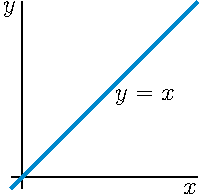
\includegraphics{fig/sec1_1_Q1a.pdf}\qquad\qquad
     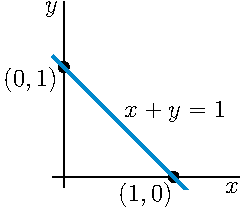
\includegraphics{fig/sec1_1_Q1b.pdf}
\end{center}

(b) $x+y=1$ is the straight line through the points $(1,0)$ and
$(0,1)$. It is sketched in the figure on the right above.

(c) $x^2+y^2=4$ is the circle with centre $(0,0)$ and radius 2. It is 
sketched in the figure on the left below.

\begin{center}
     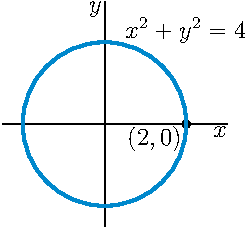
\includegraphics{fig/sec1_1_Q1c.pdf}\qquad\qquad
     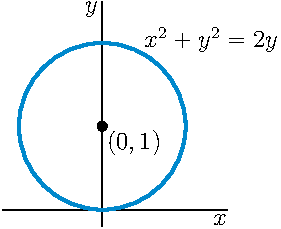
\includegraphics{fig/sec1_1_Q1d.pdf}
\end{center}

(d) $x^2+y^2=2y$ is the circle with centre $(0,1)$ and radius 1.
It is sketched in the figure on the right above.

(e) $x^2+y^2<2y$ is the set of points that are strictly inside 
the circle with centre $(0,1)$ and radius 1.
It is the shaded region (not including the dashed circle) in the sketch below.

\begin{center}
     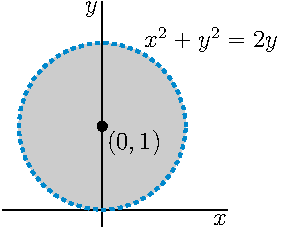
\includegraphics{fig/sec1_1_Q1e.pdf}
\end{center}

\end{answer}

\begin{solution}
(a) $x=y$ is a straight line and passes through the points $(0,0)$
and $(1,1)$. So it is the straight line through the origin that makes an angle $45^\circ$ with the $x$-- and $y$--axes. It is sketched in the figure on the 
left below.

\begin{center}
     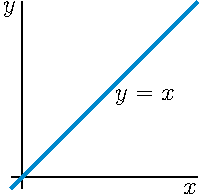
\includegraphics{fig/sec1_1_Q1a.pdf}\qquad\qquad
     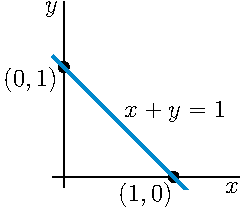
\includegraphics{fig/sec1_1_Q1b.pdf}
\end{center}

(b) $x+y=1$ is the straight line through the points $(1,0)$ and
$(0,1)$. It is sketched in the figure on the right above.

(c) $x^2+y^2$ is the square of the distance from $(0,0)$ to $(x,y)$.
So $x^2+y^2=4$ is the circle with centre $(0,0)$ and radius 2.
It is sketched in the figure on the left below.

\begin{center}
     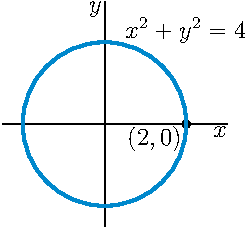
\includegraphics{fig/sec1_1_Q1c.pdf}\qquad\qquad
     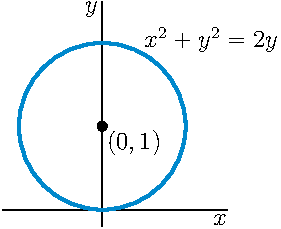
\includegraphics{fig/sec1_1_Q1d.pdf}
\end{center}

(d) The equation $x^2+y^2=2y$ is equivalent to  $x^2+(y-1)^2=1$.
As $x^2+(y-1)^2$ is the square of the distance from $(0,1)$ to $(x,y)$,
$x^2+(y-1)^2=1$ is the circle with centre $(0,1)$ and radius 1.
It is sketched in the figure on the right above.

(e) As in part (d),
\begin{equation*}
x^2+y^2<2y
\iff x^2+y^2-2y<0
\iff x^2+y^2-2y+1<1
\iff x^2+(y-1)^2<1
\end{equation*}
As $x^2+(y-1)^2$ is the square of the distance from $(0,1)$ to $(x,y)$,
$x^2+(y-1)^2<1$ is the set of points whose distance from $(0,1)$ is 
strictly less than $1$. That is, it is the set of points strictly inside 
the circle with centre $(0,1)$ and radius 1.
That set is the shaded region (not including the dashed circle) 
in the sketch below.

\begin{center}
     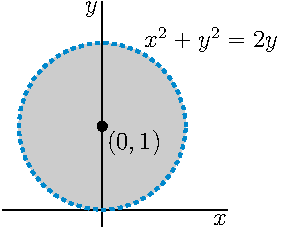
\includegraphics{fig/sec1_1_Q1e.pdf}
\end{center}
\end{solution}

%%%%%%%%%%%%%%%%%%%%%%%%%%%%%%%%%%%%%%
\begin{question}
Describe the set of all points $(x,y,z)$ in $\bbbr^3$ that satisfy
the following conditions. Sketch the part of the set that is in the 
first octant.
\begin{enumerate}[(a)]
\item
$z = x$
\item
$x + y + z = 1$
\item
$x^2 + y^2 + z^2 = 4$
\item
$x^2 + y^2 + z^2 = 4$, $z = 1$
\item
$x^2+y^2=4$
\item
$z = x^2 + y^2$
\end{enumerate}
\end{question}

%\begin{hint}
%
%\end{hint}


\begin{answer}
(a)
The set $z=x$ is the plane which contains the $y$--axis and which  
makes an angle $45^\circ$ with the $xy$--plane. Here is a sketch 
of the part of the plane that is in the first octant.

\begin{center}
     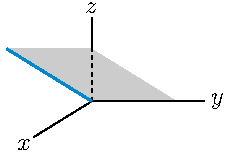
\includegraphics{fig/xeqzPlane.pdf}
\end{center}


(b)
$x+y+z=1$ is the plane through the points $(1,0,0)$, $(0,1,0)$
and  $(0,0,1)$. Here is a sketch of the part of the plane 
that is in the first octant.

\begin{center}
     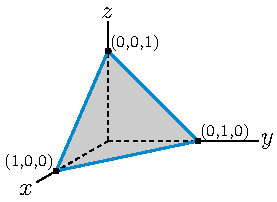
\includegraphics{fig/xyzPlane.pdf}
\end{center}


(c)
$x^2+y^2+z^2=4$ is the sphere with centre $(0,0,0)$ and radius 2.
Here is a sketch of the part of the sphere that is in the first octant.

\begin{center}
     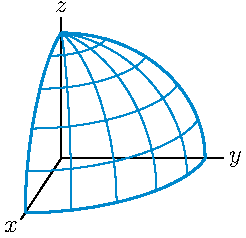
\includegraphics{fig/quarterSphere.pdf}
\end{center}

(d)
$x^2+y^2+z^2=4$, $z=1$ is the circle in the plane $z=1$ 
that has centre $(0,0,1)$ and radius $\sqrt{3}$. The part of the circle
in the first octant is the heavy quarter circle in the sketch

\begin{center}
     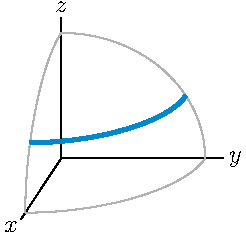
\includegraphics{fig/quarterCircle.pdf}
\end{center}


(e)
$x^2+y^2=4$ is the cylinder of radius $2$ centered on the $z$--axis.
Here is a sketch of the part of the cylinder that is in the first octant.

\begin{center}
     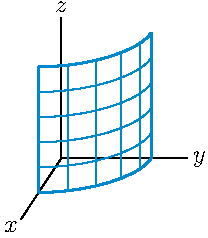
\includegraphics{fig/quarterCylinder.pdf}
\end{center}


(f) $z=x^2+y^2$ is a paraboloid consisting of a vertical stack of 
horizontal circles. The intersection of the surface with the $yz$--plane 
is the parabola $z=y^2$.  Here is a sketch of the part of the paraboloid 
that is in the first octant.

\begin{center}
     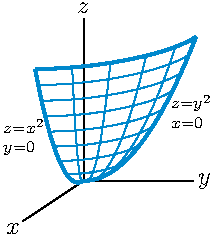
\includegraphics{fig/quarterParaboloid.pdf}
\end{center}

\end{answer}


\begin{solution}
(a) 
For each fixed $y_0$, $z=x,\ y=y_0$ is a straight line 
that lies in the plane, $y=y_0$ (which is parallel to the plane 
containing the $x$ and $z$ axes and is a distance $y_0$ from it). 
This line passes through $x=z=0$ and makes an angle $45^\circ$ 
with the $xy$--plane. Such a line (with $y_0=0$) is sketched in the 
figure below.
The set $z=x$ is the union of all the lines $z=x,\ y=y_0$ with all 
values of $y_0$. As $y_0$ varies  $z=x,\ y=y_0$ sweeps out the 
plane which contains the $y$--axis and which  makes an angle 
$45^\circ$ with the $xy$--plane. Here is a sketch of the part of the plane 
that is in the first octant.

\begin{center}
     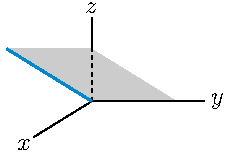
\includegraphics{fig/xeqzPlane.pdf}
\end{center}


(b) 
$x+y+z=1$ is the plane through the points $(1,0,0)$, $(0,1,0)$
and  $(0,0,1)$. Here is a sketch of the part of the plane 
that is in the first octant.

\begin{center}
     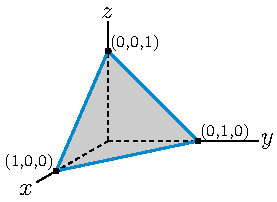
\includegraphics{fig/xyzPlane.pdf}
\end{center}

(c)
  $x^2+y^2+z^2$ is the square of the distance from $(0,0,0)$ to $(x,y,z)$.
So $x^2+y^2+z^2=4$ is the set of points whose distance from $(0,0,0)$ is
$2$. It is the sphere with centre $(0,0,0)$ and radius 2.
Here is a sketch of the part of the sphere that is in the first octant.

\begin{center}
     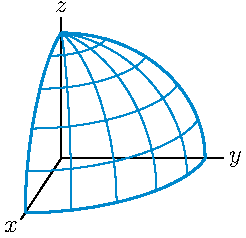
\includegraphics{fig/quarterSphere.pdf}
\end{center}

(d) 
$x^2+y^2+z^2=4$, $z=1$ or equivalently $x^2+y^2=3$, $z=1$,
is the intersection of the plane $z=1$ with the sphere of centre 
$(0,0,0)$ and radius 2. It is a circle in the plane $z=1$ 
that has centre $(0,0,1)$ and radius $\sqrt{3}$. The part of the circle
in the first octant is the heavy quarter circle in the sketch

\begin{center}
     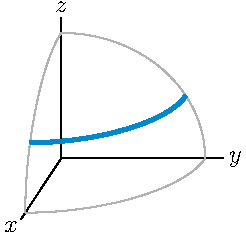
\includegraphics{fig/quarterCircle.pdf}
\end{center}

(e) 
For each fixed $z_0$, $x^2+y^2=4$, $z=z_0$ is a circle in the 
plane $z=z_0$ with centre $(0,0,z_0)$ and radius $2$. 
So $x^2+y^2=4$ is the union of $x^2+y^2=4,\ z=z_0$ for all 
possible values of $z_0$. It is  a vertical stack of horizontal 
circles. It is the cylinder of radius $2$ centered on the $z$--axis.
Here is a sketch of the part of the cylinder that is in the first octant.

\begin{center}
     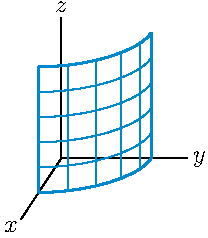
\includegraphics{fig/quarterCylinder.pdf}
\end{center}


(f)
For each fixed $z_0\ge 0$, the curve $z = x^2 + y^2,\ z=z_0$ is the circle in the plane $z=z_0$ with centre $(0,0,z_0)$ and radius $\sqrt{z_0}$. As 
$z = x^2 + y^2$ is the union of $z = x^2 + y^2,\ z=z_0$ for all 
possible values of $z_0\ge 0$, it is  a vertical stack of horizontal circles.
The intersection of the surface with the $yz$--plane is the parabola
$z=y^2$.  Here is a sketch of the part of the paraboloid that is in the 
first octant.

\begin{center}
     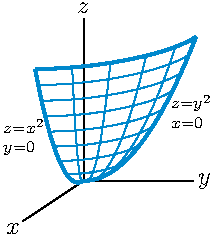
\includegraphics{fig/quarterParaboloid.pdf}
\end{center}


\end{solution}




%%%%%%%%%%%%%%%%%%
\subsection*{\Procedural}
%%%%%%%%%%%%%%%%%%

\begin{question}
The pressure $p(x,y)$ at the point $(x,y)$ is determined by 
$x^2-2px+y^2=1$. Sketch several isobars. An isobar is a curve with
equation $p(x,y)=c$ for some constant $c$.
\end{question}

%\begin{hint}
%
%\end{hint}


\begin{answer}
\begin{center}
     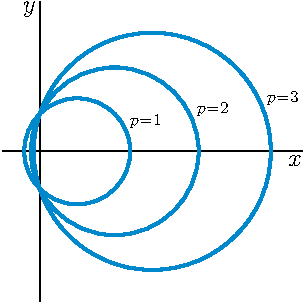
\includegraphics{fig/pressure.pdf}
\end{center}

\end{answer}


\begin{solution}
For each fixed $c$, the isobar $p(x,y)=c$ is the curve
$x^2-2cx+y^2=1$, or equivalently, $(x-c)^2+y^2=1+c^2$. This is a 
circle with centre $(c,0)$ and radius $\sqrt{1+c^2}$, which for large $c$ is just a bit bigger than $c$.

\begin{center}
     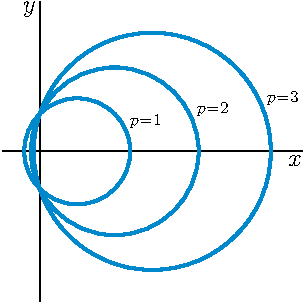
\includegraphics{fig/pressure.pdf}
\end{center}


\end{solution}


%%%%%%%%%%%%%%%%%%%%%%%%%
\begin{question}
Consider any triangle. Pick a coordinate system so that one vertex
is at the origin and a second vertex is on the positive $x$--axis. Call
the coordinates of the second vertex $(a,0)$ and those of the third vertex
$(b,c)$. Find the circumscribing circle (the circle that goes through all
three vertices).
\end{question}

%\begin{hint}
%
%\end{hint}


\begin{answer}
The circumscribing circle has centre $(\bar x,\bar y)$ and radius $r$
with $\bar x=\frac{a}{2}$, $\bar y=\frac{b^2+c^2-ab}{2c}$ and
$r=\sqrt{\big(\frac{a}{2}\big)^2+\big(\frac{b^2+c^2-ab}{2c}\big)^2}$.
\end{answer}


\begin{solution}
Call the centre of the circumscribing circle 
$(\bar x,\bar y)$. This centre must be equidistant from the three vertices.
So
\begin{equation*}
\bar x^2+\bar y^2=(\bar x-a)^2+\bar y^2=(\bar x-b)^2+(\bar y-c)^2 
\end{equation*}
or, subtracting $\bar x^2+\bar y^2$ from the three equal expressions,
\begin{equation*}
0=a^2-2a\bar x=b^2-2b\bar x+c^2-2c\bar y
\end{equation*}
which implies
\begin{equation*}
\bar x=\frac{a}{2}\qquad\qquad \bar y
=\frac{b^2+c^2-2b\bar x}{2c}=\frac{b^2+c^2-ab}{2c}
\end{equation*}
The radius is the distance from the vertex $(0,0)$ to the centre 
$(\bar x,\bar y)$, which is
$\sqrt{\big(\frac{a}{2}\big)^2+\big(\frac{b^2+c^2-ab}{2c}\big)^2}$.

\end{solution}

%%%%%%%%%%%%%%%%%%%%%%%%%%%%%%%%%%%%%%%%%
\begin{question} [M200 2001A] % 1
A certain quadric surface consists of all points $P=(x,y,z)$
such that the distance from $P$ to the point $(0,0,1)$ is equal to the
distance from $P$ to the plane $z+1=0$. Find an equation for the surface,
sketch and describe it verbally.
\end{question}

%\begin{hint}
%
%\end{hint}

\begin{answer}
$x^2+y^2=4z$
The surface is a paraboloid consisting of a stack of horizontal circles, starting with a point at the origin and with radius increasing vertically.
The circle in the plane $z=z_0$ has radius $2\sqrt{z_0}$.
\end{answer}

\begin{solution}
The distance from $P$ to the point $(0,0,1)$ is $\sqrt{x^2+y^2+(z-1)^2}$.
The distance from $P$ to the specified plane is $|z+1|$. Hence the equation
of the surface is
\begin{equation*}
x^2+y^2+(z-1)^2=(z+1)^2\text{ or }
   x^2+y^2=4z
\end{equation*}
All points on this surface have $z\ge 0$. The set of points on the surface
that have any fixed value, $z_0\ge 0$, of $z$ consists of a circle that is
centred on the $z$--axis, is parallel to the $xy$-plane and has radius
$2\sqrt{z_0}$. The surface consists of a stack of these circles, starting
with a point at the origin and with radius increasing vertically. The surface
is a paraboloid and is sketched below.
\begin{center}
     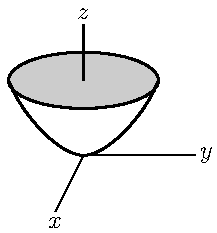
\includegraphics{fig/OE01AQ1.pdf}
\end{center}
\end{solution}









%%%%%%%%%%%%%%%%%%
%\subsection*{\Application}
%%%%%%%%%%%%%%%%%%

\section{Vectors}
%\documentclass\llt 12pt]{article}

\questionheader{ex:s1.2}


%%%%%%%%%%%%%%%%%%
\subsection*{\Conceptual}
%%%%%%%%%%%%%%%%%%

%%%%%%%%%%%%%%%%%%%%%%%%%%%%%%%%%%%%
\begin{question}
Let $\va=\llt 2,0\rgt $ and $\vb=\llt 1,1\rgt $. Evaluate and sketch
$\va+\vb,\ \va+2\vb$ and $2\va-\vb$.
\end{question}

%\begin{hint}
%\end{hint}

\begin{answer}
$\va+\vb=\llt 3,1\rgt $, $\va+2\vb=\llt 4,2\rgt $,\ 
$2\va-\vb=\llt 3,-1\rgt $

\begin{center}
     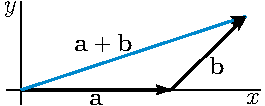
\includegraphics{add1.pdf}\qquad
     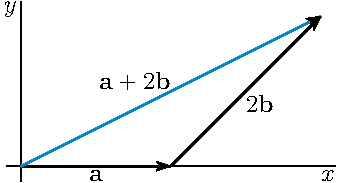
\includegraphics{add2.pdf}
\end{center}
\begin{center}
     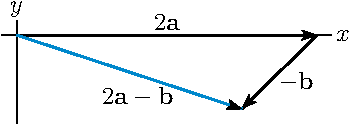
\includegraphics{add3.pdf}
\end{center}

\end{answer}

\begin{solution}
$\va+\vb=\llt 3,1\rgt $, $\va+2\vb=\llt 4,2\rgt $,\ 
$2\va-\vb=\llt 3,-1\rgt $

\begin{center}
     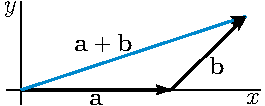
\includegraphics{add1.pdf}\qquad
     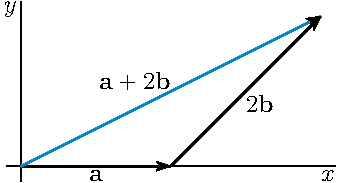
\includegraphics{add2.pdf}
\end{center}
\begin{center}
     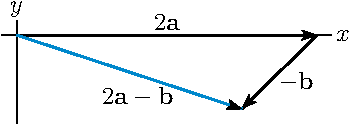
\includegraphics{add3.pdf}
\end{center}

\end{solution}

%%%%%%%%%%%%%%%%%%%%%%%%%%%%%%%%%%%%
\begin{question}
Determine whether or not the given points are collinear (that is, 
lie on a common straight line)
\begin{enumerate}[(a)]
\item
 $(1,2,3),\ (0,3,7),\ (3,5,11)$

\item
$(0,3,-5),\ (1,2,-2),\ (3,0,4)$
\end{enumerate}
\end{question}

\begin{hint}
If three points are collinear, then the vector from the first point
to the second point, and the vector from the first point to the third point 
must both be parallel to the line, and hence must be parallel to each other
(i.e. must be multiples of each other).

\begin{center}
     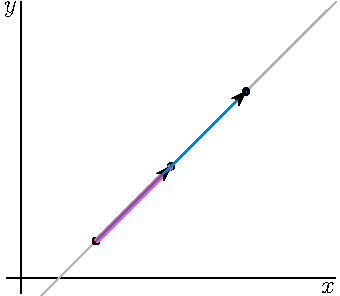
\includegraphics{collinear.pdf}
\end{center}

\end{hint}

\begin{answer}
(a) not collinear\qquad
(b) collinear
\end{answer}

\begin{solution}
If three points are collinear, then the vector from the first point
to the second point, and the vector from the first point to the third point 
must both be parallel to the line, and hence must be parallel to each other
(i.e. must be multiples of each other).

\begin{center}
     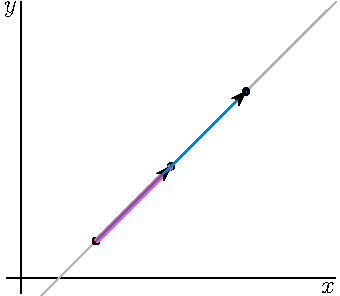
\includegraphics{collinear.pdf}
\end{center}

(a)
The vectors $\llt 0,3,7\rgt -\llt 1,2,3\rgt =\llt -1,1,4\rgt $ and $\llt 3,5,11\rgt -\llt 1,2,3\rgt =\llt 2,3,8\rgt $ 
are not parallel (i.e. are not multiples of each other),
so the three points are not on the same line.

(b)
The vectors $\llt 1,2,-2\rgt -\llt 0,3,-5\rgt =\llt 1,-1,3\rgt $ and
$\llt 3,0,4\rgt -\llt 0,3,-5\rgt =\llt 3,-3,9\rgt $ are parallel (i.e. are  multiples of each other),
so the three points are on the same line.
\end{solution}

%%%%%%%%%%%%%%%%%%%%%%%%%%%%%%%%
\begin{question}
Determine whether the given pair of vectors is perpendicular
\begin{enumerate}[(a)]
\item
$\llt 1,3,2\rgt ,\ \llt 2,-2,2\rgt $ 
\item
$\llt -3,1,7\rgt ,\ \llt 2,-1,1\rgt $ 
\item
$\llt 2,1,1\rgt ,\ \llt -1,4,2\rgt $ 
\end{enumerate}
\end{question}

\begin{hint}
Review Theorem \eref{CLP200}{thm:dotPppties} in the CLP-3 text.
\end{hint}

\begin{answer}
(a) perpendicular\qquad
(b) perpendicular\qquad
(c) not perpendicular
\end{answer}

\begin{solution}
\leqnomode
By property 7 of Theorem \eref{CLP200}{thm:dotPppties} in the CLP-3 text,
\begin{alignat*}{3}
\llt 1,3,2\rgt \cdot\llt 2,-2,2\rgt 
&=1\times2-3\times 2+2\times2=0\ 
&&\implies\ \text{perpendicular}
\tag{a} \\
\llt -3,1,7\rgt \cdot\llt 2,-1,1\rgt 
&=-3\times2-1\times 1+7\times1=0\ 
&&\implies\ \text{perpendicular}
\tag{b} \\
\llt 2,1,1\rgt \cdot\llt -1,4,2\rgt 
&=-2\times1+1\times 4+1\times2=4\ne 0\ 
&&\implies\ \text{not perpendicular}
\tag{c}
\end{alignat*}
\reqnomode
\end{solution}

%%%%%%%%%%%%%%%%%%%%%%%%%%%%%%%%%%%%
\begin{question}
Let $\va=\llt a_1,a_2\rgt$. Compute the projection of $\va$ on
$\hi$ and $\hj$.
\end{question}

%\begin{hint}
%\end{hint}

\begin{answer}
$\text{proj}_{\hi}\va=a_1\hi$\qquad
$\text{proj}_{\hj}\va=a_2\hj$.
\end{answer}

\begin{solution}
$\text{proj}_{\hi}\va=(\va\cdot\hi)\hi
=a_1\hi$ and
$\text{proj}_{\hj}\va=(\va\cdot\hj)\hj
=a_2\hj$.
\end{solution}

%%%%%%%%%%%%%%%%%%%%%%%%%%%%%%%%%%%%
\begin{question}
Does the triangle with vertices $(1,2,3),\ (4,0,5)$ and $(3,6,4)$
have a right angle?
\end{question}

%\begin{hint}
%\end{hint}

\begin{answer}
Yes.
\end{answer}

\begin{solution}
The vector from $(1,2,3)$ to $(4,0,5)$ is $\llt 3,-2,2\rgt$.
The vector from $(1,2,3)$ to $(3,6,4)$ is $\llt 2,4,1\rgt$.
The dot product between these two vectors is 
$\llt 3,-2,2\rgt\cdot\llt 2,4,1\rgt=0$,
so the vectors are perpendicular and the triangle does contain a right
angle.

\end{solution}

%%%%%%%%%%%%%%%%%%%%%%%%%%%%%
\begin{question}
Show that the area of the parallelogram determined by the
vectors $\va$ and $\vb$ is $|\va\times \vb|$.

\begin{center}
     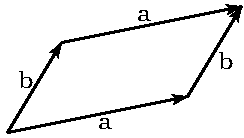
\includegraphics{sec_1_2_pgramA.pdf}
\end{center}

\end{question}

%\begin{hint}
%\end{hint}

\begin{answer}
See the solution.
\end{answer}

\begin{solution}
 The area of a parallelogram is the length of its
base time its height. 
\vadjust{
\begin{center}
     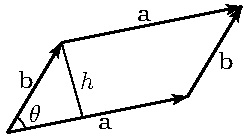
\includegraphics{sec_1_2_pgramB.pdf}
\end{center}
}%
We can choose the base to be $\va$. Then, if $\theta$
is the angle between its sides $\va$ and $\vb$, its height is 
$|\vb|\sin\theta$.  
So
\begin{equation*}
\text{area} = |\va||\vb|\sin\theta=|\va\times\vb|
\end{equation*}
\end{solution}

%%%%%%%%%%%%%%%%%%%%%%%%%%%%%
\begin{question}
Show that the volume of the parallelepiped determined by the
vectors $\va,\ \vb$ and $\vc$ is 
\begin{equation*}
    |\va\cdot(\vb\times\vc)|
\end{equation*}

\begin{center}
     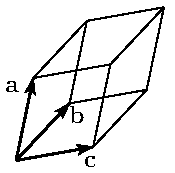
\includegraphics{piped.pdf}
\end{center}

\end{question}

%\begin{hint}
%\end{hint}

\begin{answer}
See the solution
\end{answer}

\begin{solution}
The volume of a parallelepiped is the area of its
base time its height. We can choose the base to be the parallelogram 
determined by the vectors $\vb$ and $\vc$. It has area $|\vb\times\vc|$.
The vector $\vb\times\vc$ is perpendicular to the base. 
\vadjust{
\begin{center}
     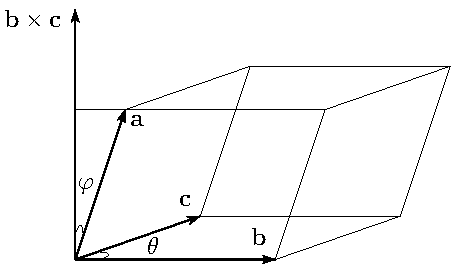
\includegraphics{pipedVolume.pdf}
\end{center}
}%
Denote by
$\theta$ the angle between $\va$ and the perpendicular $\vb\times\vc$.
The height of the parallelepiped is $|\va| |\cos\theta|$. So 
\begin{equation*}
\text{volume} = |\va|\, |\cos\theta|\, |\vb\times\vc|
=|\va\cdot(\vb\times\vc)|
\end{equation*}
\end{solution}

%%%%%%%%%%%%%%%%%%%%%%%%%%%%%%%%
\begin{question}
Verify by direct computation that
\begin{enumerate}[(a)]
\item
$\hi\times\hj=\hk$, $\hj\times\hk=\hi$, $\hk\times\hi=\hj$
\item
$\va\cdot(\va\times\vb)=\vb\cdot(\va\times\vb)=\vZero$
\end{enumerate}
\end{question}

%\begin{hint}
%
%\end{hint}

\begin{answer}
See the solution.
\end{answer}

\begin{solution}
(a)
\begin{alignat*}{5}
\hi\times\hj&=\det\left[\begin{matrix}\hi&\hj &\hk\\
                     1&0&0\\
                     0&1&0\end{matrix}\right]
&&=\hi(0\times 0-0\times 1)
-\hj(1\times 0-0\times 0)
+\hk(1\times 1-0\times 0) \\
&=\hk\\[0.1in]
%%
\hj\times\hk&=\det\left[\begin{matrix}\hi&\hj &\hk\\
                     0&1&0\\
                     0&0&1\end{matrix}\right]
&&=\hi(1\times 1-0\times 0)
-\hj(0\times 1-0\times 0)
+\hk(0\times 0-1\times 0)\\
&=\hi\\[0.1in]
%%
\hk\times\hi&=\det\left[\begin{matrix}\hi&\hj &\hk\\
                     0&0&1\\
                     1&0&0\end{matrix}\right]
&&=\hi(0\times 0-1\times 0)
-\hj(0\times 0-1\times 1)
+\hk(0\times 0-0\times 1)\\
&=\hj
\end{alignat*}

(b)
\begin{alignat*}{5}
\va\cdot(\va\times\vb)
&=a_1\big(a_2b_3-a_3b_2\big)
  -a_2\big(a_1b_3-a_3b_1\big)
  +a_3\big(a_1b_2-a_2b_1\big)
&&=0\\
\vb\cdot(\va\times\vb)
&=b_1\big(a_2b_3-a_3b_2\big)
  -b_2\big(a_1b_3-a_3b_1\big)
  +b_3\big(a_1b_2-a_2b_1\big)
&&=0
\end{alignat*}
\end{solution}




%%%%%%%%%%%%%%%%%%%%%%%%%%%%%%%%
\begin{question}
Consider the following statement: ``If $\va\ne\vZero$
and if $\va\cdot\vb=\va\cdot\vc$ then $\vb=\vc$.''
If the statment is true, prove it. If the statement is false, give a 
counterexample.
\end{question}

%\begin{hint}
%
%\end{hint}

\begin{answer}
This statement is false. One counterexample is $\va=\llt 1,0,0\rgt $,
$\vb=\llt 0,1,0\rgt ,\ \vc=\llt 0,0,1\rgt $. Then $\va\cdot\vb=\va\cdot\vc=0$, but $\vb\ne\vc$. There are \emph{many} other counterexamples.
\end{answer}

\begin{solution}
This statement is false. The two numbers 
$\va\cdot\vb$, $\va\cdot\vc$ are equal if and only if
$\va\cdot(\vb-\vc)= 0$. This in turn is the case if and only
if $\va$ is perpendicular to $\vb-\vc$ (under the convention that
$\vZero$ is perpendicular to all vectors). For example, 
if $\va=\llt 1,0,0\rgt $, $\vb=\llt 0,1,0\rgt ,\ \vc=\llt 0,0,1\rgt $, then $\vb-\vc=\llt 0,1,-1\rgt$ is perpendicular to $\va$ so that 
$\va\cdot\vb=\va\cdot\vc$.
\end{solution}

%%%%%%%%%%%%%%%%%%%%%%%%%%%%%%%%%%%%
\begin{question}\label{PRB Qnine}
Consider the following statement: ``The vector $\va\times(\vb\times\vc)$ 
is of the form $\al\vb+\be\vc$ for some real numbers $\al$ and $\be$.''
If the statement is true, prove it. If the statement is false, give a 
counterexample.

\end{question}

%\begin{hint}
%\end{hint}

\begin{answer}
True.
\end{answer}

\begin{solution}
This statement is true. In the event that $\vb$ and 
$\vc$ are parallel, $\vb\times\vc=\vZero$ so that
$\va\times(\vb\times\vc)=\vZero=0\vb+0\vc$, so we may assume
that $\vb$ and $\vc$ are not parallel. Then as $\al$ and $\be$ run
over $\bbbr$, the vector $\al\vb+\be \vc$ runs over the plane that
contains the origin and the vectors $\vb$ and $\vc$. Call this plane
$P$. Because
$\vd=\vb\times\vc$ is nonzero and perpendicular to both 
$\vb$ and $\vc$, $P$ is the plane that contains the origin
and is perpendicular to $\vd$. As $\va\times(\vb\times\vc)=\va\times\vd$ is always perpendicular to $\vd$, it lies in $P$.
\end{solution}

%%%%%%%%%%%%%%%%%%%%%%%%%%%%%%%%%%%%
\begin{question}
What geometric conclusions can you draw from
$\va\cdot(\vb\times\vc)=\llt 1,2,3\rgt$?
\end{question}

%\begin{hint}
%\end{hint}

\begin{answer}
None. The given equation is nonsense.
\end{answer}

\begin{solution}
None. The given equation is nonsense. The left hand side is
a number while the right hand side is a vector.
\end{solution}

%%%%%%%%%%%%%%%%%%%%%%%%%%%%%%%%%%%%
\begin{question}
What geometric conclusions can you draw from
$\va\cdot(\vb\times\vc)=0$?
\end{question}

%\begin{hint}
%\end{hint}

\begin{answer}
If $\vb$ and $\vc$ are parallel, then $\va\cdot(\vb\times\vc)=0$ for all $\va$.
If $\vb$ and $\vc$ are not parallel, then $\va$ must be of the form  
$\al\vb+\be\vc$ with $\al$ and $\be$ real numbers.
\end{answer}

\begin{solution}
If $\vb$ and $\vc$ are parallel, then $\vb\times\vc=\vZero$
and $\va\cdot(\vb\times\vc)=0$ for all $\va$.
If $\vb$ and $\vc$ are not parallel, $\va\cdot(\vb\times\vc)=0$ 
if and only if $\va$ is perpendicular to $\vd=\vb\times\vc$.
As we saw in question \ref{PRB Qnine}, the set of all vectors perpendicular to
$\vd$ is the plane consisting of all vectors of the form  
$\al\vb+\be\vc$ with $\al$ and $\be$ real numbers. So $\va$ must
be of this form.
\end{solution}

%%%%%%%%%%%%%%%%%%%%%%%%%%%%%%%%%%%%
\begin{question}
Consider the three points $O=(0,0)$, $A=(a,0)$ and $B=(b,c)$.
\begin{enumerate}[(a)]
\item
Sketch, in a single figure,
\begin{itemize}\itemsep1pt \parskip0pt \parsep0pt %\itemindent-15pt
\item
the triangle with vertices $O$, $A$ and $B$, and
\item
the circumscribing circle for the triangle (i.e. the circle that goes 
through all three vertices), and
\item
the vectors
\begin{itemize}\itemsep1pt \parskip0pt \parsep0pt %\itemindent-15pt
\item 
$\overrightarrow{OA}$, from $O$ to $A$,
\item 
$\overrightarrow{OB}$, from $O$ to $B$,
\item 
$\overrightarrow{OC}$, from $O$ to $C$, where $C$ is the centre of the circumscribing circle.
\end{itemize}
\end{itemize}
Then add to the sketch and evaluate, from the sketch,
\begin{itemize}\itemsep1pt \parskip0pt \parsep0pt %\itemindent-15pt
\item 
the projection of the vector $\overrightarrow{OC}$ on the vector 
$\overrightarrow{OA}$, and
\item 
the projection of the vector $\overrightarrow{OC}$ on the vector 
$\overrightarrow{OB}$.
\end{itemize}

\item Determine $C$.

\item
Evaluate, using the formula (\eref{CLP200}{eqn proj}) in the CLP-3 text,
\begin{itemize}\itemsep1pt \parskip0pt \parsep0pt %\itemindent-15pt
\item 
the projection of the vector $\overrightarrow{OC}$ on the vector 
$\overrightarrow{OA}$, and
\item 
the projection of the vector $\overrightarrow{OC}$ on the vector 
$\overrightarrow{OB}$.
\end{itemize}
\end{enumerate}
\end{question}

\begin{hint}
(a)
The three line segments from $C$ to $O$, from $C$ to $A$ and from $C$ to $B$
all have exactly the same length, namely the radius of the circumscribing 
circle.

(b) 
Let $(\bar x,\bar y)$ be the coordinates of $C$.
Write down the equations that say that $(\bar x,\bar y)$ is
equidistant from the three vertices $O$, $A$ and $B$.
\end{hint}

\begin{answer}
(a), (c)
\begin{center}
     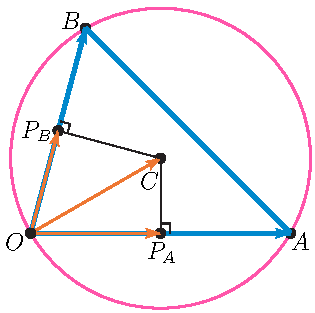
\includegraphics{circumA.pdf}
\end{center}
$\text{proj}_{\overrightarrow{\scriptstyle OA}}\,\overrightarrow{OC}
    =\overrightarrow{OP_A}=\llt a/2,0\rgt$\qquad
$\text{proj}_{\overrightarrow{\scriptstyle OB}}\,\overrightarrow{OC}
    =\overrightarrow{OP_A}=\llt b/2,c/2\rgt$

(b) The centre of the circumscribing circle is $(\bar x,\bar y)$ with
$\bar x=\frac{a}{2}$ and
$ \bar y =\frac{b^2+c^2-ab}{2c}$.
\end{answer}

\begin{solution}
(a) The sketch for part (a) is on the left below.
To sketch the projections, we dropped perpendiculars 
\begin{itemize}\itemsep1pt \parskip0pt \parsep0pt %\itemindent-15pt
\item 
from $C$ to the line from $O$ to $A$, and 
\item 
from $C$ to the line from $O$ to $B$.
\end{itemize}
By definition, 
\begin{itemize}\itemsep1pt \parskip0pt \parsep0pt %\itemindent-15pt
\item 
$\text{proj}_{\overrightarrow{\scriptstyle OA}}\,\overrightarrow{OC}$
is the vector $\overrightarrow{OP_A}$ from $O$ to the point $P_A$, where 
the perpendicular from $C$ to the line from $O$ to $A$ hits the line,
and 
\item 
$\text{proj}_{\overrightarrow{\scriptstyle OB}}\,\overrightarrow{OC}$
is the vector $\overrightarrow{OP_B}$ from $O$ to the point $P_B$, where 
the perpendicular from $C$ to the line from $O$ to $B$ hits the line.
\end{itemize}
\begin{center}
     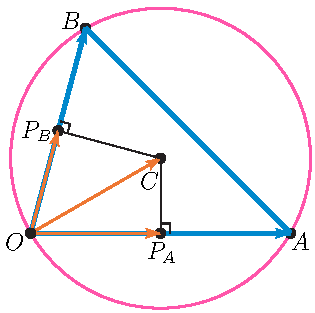
\includegraphics{circumA.pdf}\qquad\qquad
     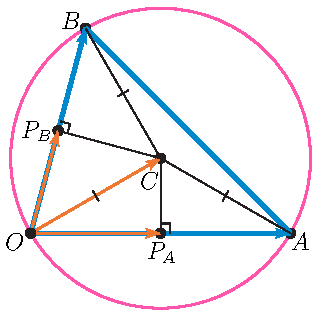
\includegraphics{circum.pdf}
\end{center}
To evaluate the projections we observe that the three lines from 
$C$ to $O$, from $C$ to $A$ and from $C$ to $B$ all have exactly the same length
(namely the radius of the circumscribing circle). Consequently
(see the figure on the right above),
\begin{itemize}\itemsep1pt \parskip0pt \parsep0pt %\itemindent-15pt
\item 
the triangle $OCA$ is an isoceles triangle, so that $P_A$ is exactly the
midpoint of the line segement from $O$ to $A$. That is, $P_A$ is $(a/2,0)$ and
\begin{equation*}
\text{proj}_{\overrightarrow{\scriptstyle OA}}\,\overrightarrow{OC}
    =\overrightarrow{OP_A}=\llt a/2,0\rgt
\end{equation*}
\item 
Similarly, the triangle $OCB$ is an isoceles triangle, so that $P_B$ is 
exactly the midpoint of the line segement from $O$ to $B$. That is $P_A$ is $(b/2,c/2)$ and
\begin{equation*}
\text{proj}_{\overrightarrow{\scriptstyle OB}}\,\overrightarrow{OC}
    =\overrightarrow{OP_B}=\llt b/2,c/2\rgt
\end{equation*}
\end{itemize}

(b)
Call the centre of the circumscribing circle $(\bar x,\bar y)$. 
This centre must be equidistant from the three vertices.
So
\begin{align*}
\bar x^2+\bar y^2=(\bar x-a)^2+\bar y^2=(\bar x-b)^2+(\bar y-c)^2 
\end{align*}
or, subtracting $\bar x^2+\bar y^2$ from all three expression,
\begin{align*}
0=a^2-2a\bar x=b^2-2b\bar x+c^2-2c\bar y
\end{align*}
which implies
\begin{equation*}
\bar x=\frac{a}{2}\qquad\qquad \bar y
=\frac{b^2+c^2-2b\bar x}{2c}=\frac{b^2+c^2-ab}{2c}
\end{equation*}


(c) From part (b), we have
\begin{align*}
\overrightarrow{OA}\cdot\overrightarrow{OC}
&=\llt a,0\rgt\cdot\llt\frac{a}{2}\,,\,\frac{b^2+c^2-ab}{2c}\rgt
=\frac{a^2}{2}=\frac{1}{2}|\overrightarrow{OA}|^2\\
\overrightarrow{OB}\cdot\overrightarrow{OC}
&=\llt b,c\rgt\cdot\llt\frac{a}{2}\,,\,\frac{b^2+c^2-ab}{2c}\rgt
=\frac{ab}{2}+\frac{b^2+c^2-ab}{2}=\frac{b^2+c^2}{2}
=\frac{1}{2}|\overrightarrow{OB}|^2 
\end{align*}
So, by Equation (\eref{CLP200}{eqn proj}) in the CLP-3 text,
\begin{align*}
\text{proj}_{\overrightarrow{\scriptstyle OA}}\,\overrightarrow{OC}
&=\frac{\overrightarrow{OA}\cdot\overrightarrow{OC}}{|\overrightarrow{OA}|^2}
           \overrightarrow{OA}
=\frac{1}{2}\overrightarrow{OA}
=\llt a/2,0\rgt \\
\text{proj}_{\overrightarrow{\scriptstyle OB}}\,\overrightarrow{OC}
&=\frac{\overrightarrow{OB}\cdot\overrightarrow{OC}}{|\overrightarrow{OB}|^2}
           \overrightarrow{OB}
=\frac{1}{2}\overrightarrow{OB}
=\llt b/2,c/2\rgt
\end{align*}


\end{solution}






%%%%%%%%%%%%%%%%%%%%%%%%%%%%
%\Instructions{Questions~\ref{prob_s1.0first} through \ref{prob_s1.0last} provide practice with.}
%%%%%%%%%%%%%%%%%%%%

%%%%%%%%%%%%%%%%%%
\subsection*{\Procedural}
%%%%%%%%%%%%%%%%%%

%%%%%%%%%%%%%%%%%%%%%%%%%%%%%%%%%%%%
\begin{question}
Find the equation of a sphere if one of its diameters has end
points $(2,1,4)$ and $(4,3,10)$.
\end{question}

\begin{hint}
The centre of the sphere is the midpoint of the diameter.
\end{hint}

\begin{answer}
$(x-3)^2+(y-2)^2+(z-7)^2=11$
\end{answer}

\begin{solution}
The center of the sphere is 
$\half\big\{(2,1,4)+(4,3,10)\big\}=(3,2,7)$. The diameter (i.e. twice the radius) is $|(2,1,4)-(4,3,10)|=|(-2,-2,-6)|=2|(1,1,3)|=2\sqrt{11}$. So the radius of the sphere is $\sqrt{11}$ and
the equation of the sphere is
\begin{equation*}
(x-3)^2+(y-2)^2+(z-7)^2=11
\end{equation*}
\end{solution}

%%%%%%%%%%%%%%%%%%%%%%%%%%%%%%%%%%%%
\begin{question}
Show that the set of all points $P$ that are twice as far from
$(3,-2,3)$ as from $(3/2,1,0)$ is a sphere. Find its centre and radius.
\end{question}

%\begin{hint}
%\end{hint}

\begin{answer}
The sphere has radius 3 and is centered on $(1,2,-1)$.
\end{answer}

\begin{solution}
Let $(x,y,z)$ be a point in $P$. The distances from
$(x,y,z)$ to $(3,-2,3)$ and to $(3/2,1,0)$ are 
\begin{equation*}
\sqrt{(x-3)^2+(y+2)^2+(z-3)^2}\quad\text{ and }\quad
\sqrt{(x-3/2)^2+(y-1)^2+z^2}
\end{equation*}
respectively. To be in $P$, $(x,y,z)$ must obey
\begin{align*}
\sqrt{(x-3)^2+(y+2)^2+(z-3)^2}&=2\sqrt{(x-3/2)^2+(y-1)^2+z^2} \\
(x-3)^2+(y+2)^2+(z-3)^2&=4(x-3/2)^2+4(y-1)^2+4z^2 \\
x^2-6x+9+y^2+4y+4+z^2-6z+9&=4x^2-12x+9+4y^2-8y+4+4z^2 \\
3x^2-6 x+3y^2-12y+3z^2+6z-9&=0 \\
x^2-2 x+y^2-4y+z^2+2z-3&=0 \\
(x-1)^2+(y-2)^2+(z+1)^2&=9
\end{align*}
This is a sphere of radius 3 centered on $(1,2,-1)$.
\end{solution}

%%%%%%%%%%%%%%%%%%%%%%%%%%%%%%%%%%%%
\begin{question}
Use vectors to prove that the line joining the midpoints of two sides
of a triangle is parallel to the third side  and half its length.
\end{question}

\begin{hint}
Draw a sketch.
Call the vertices of the triangle $A$, $B$ and $C$ with $C$ being the
vertex that joins the two sides. Let $\va$ be the vector from $C$ to $A$ 
and $\vb$ be the vector from $C$ to $B$. Determine, in terms of $\va$ and 
$\vb$, 
\begin{itemize}\itemsep0pt \parskip0pt \parsep0pt %\itemindent-15pt

\item 
the vector from $A$ to $B$, 
\item
the two vectors from $C$ to the two midpoints and finally 
\item
the vector joining the two midpoints. 
\end{itemize}
\end{hint}

\begin{answer}
See the solution.
\end{answer}

\begin{solution}
Call the vertices of the triangle $A$, $B$ and $C$ with $C$ being the
vertex that joins the two sides. We can always
choose our coordinate system so that $C$ is at the origin.
Let $\va$ be the vector from $C$ to $A$ 
and $\vb$ be the vector from $C$ to $B$.
\begin{center}
     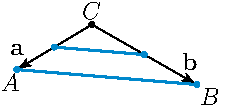
\includegraphics{triangleMidPt.pdf}
\end{center}
\begin{itemize}
\item
Then the vector from $C$ to the midpoint of the side from $C$ to $A$ is
$\half\va$ and
\item
the vector from $C$ to the midpoint of the side from $C$ to $B$ is
$\half\vb$ so that
\item
the vector joining the two midpoints is $\half\vb-\half\va$. 
\end{itemize}
As the vector from $A$ to $B$ is $\vb-\va=2\big[\half\vb-\half\va\big]$,
the line joining the midpoints is indeed parallel to the third side
and half its length.
\end{solution}


%%%%%%%%%%%%%%%%%%%%%%%%%%%%%%%%
\begin{question}
Compute the areas of the parallelograms determined by the
following vectors.
\begin{enumerate}[(a)]
\item
$\llt -3,1\rgt,\ \llt 4,3\rgt$ 
\item
$\llt 4,2\rgt,\ \llt 6,8\rgt$
\end{enumerate}
\end{question}

\begin{hint}
Review \S\eref{CLP200}{sec:GEOparallelogram} in the CLP-3 text.
\end{hint}

\begin{answer}
(a) $13$\qquad
(b) $20$
\end{answer}

\begin{solution} (a)
By (\eref{CLP200}{eq pgram area}) in the CLP-3 text, the area is 
\begin{align*}
\left| \det\left[\begin{matrix}-3&1 \\ 4&3 \end{matrix}\right] \right|
  &=\big|-3\times 3-1\times 4\big| = |-13| = 13
\end{align*}

(b)
By (\eref{CLP200}{eq pgram area}) in the CLP-3 text, the area is 
\begin{align*}
\left|\det\left[\begin{matrix} 4&2 \\ 6&8 \end{matrix}\right]\right| 
&=\big|4\times 8-2\times 6\big| 
= 20
\end{align*}
\end{solution}

\begin{question}[M200 2014A] %1c
Consider the plane $W$, defined by:
\begin{equation*}
W\ :\ -x + 3y + 3z = 6,\qquad
\end{equation*}
Find the area of the parallelogram on $W$ defined by 
$0 \le x \le 3$, $0 \le y \le 2$.
\end{question}

\begin{hint}
Determine the four corners of the parallelogram.
\end{hint}

\begin{answer}
$2\sqrt{19}$
\end{answer}

\begin{solution}
Note that 
\begin{itemize}
   \item the point on $W$ with $x=0$, $y=0$ obeys 
                         $-0+3(0)+3z=6$ and so has $z=2$
   \item the point on $W$ with $x=0$, $y=2$ obeys 
                         $-0+3(2)+3z=6$ and so has $z=0$
   \item the point on $W$ with $x=3$, $y=0$ obeys 
                         $-3+3(0)+3z=6$ and so has $z=3$
   \item the point on $W$ with $x=3$, $y=2$ obeys 
                         $-3+3(2)+3z=6$ and so has $z=1$
\end{itemize}
So the four corners of the parallelogram are 
$(0,0,2)$, $(0,2,0)$, $(3,0,3)$ and $(3,2,1)$. The vectors
\begin{align*}
\vd_1&=\llt 0-0 \,,\, 2-0 \,,\, 0-2 \rgt = \llt 0 \,,\, 2 \,,\, -2\rgt \\
\vd_2&=\llt 3-0 \,,\, 0-0 \,,\, 3-2 \rgt = \llt 3 \,,\, 0 \,,\, 1\rgt 
\end{align*}
form two sides of the paralleogram. So the area of the parallelogram is
\begin{align*}
\big|\vd_1\times\vd_2\big| 
=\left|\det\left[\begin{matrix}
                     \hi & \hj & \hk \\
                     0   &  2  & -2 \\
                     3   &  0  &  1
                \end{matrix}\right]\right|
=\left| 2\,\hi - 6\,\hj -6\hk  \right|
=\sqrt{76}
=2\sqrt{19}
\end{align*}

\end{solution}

%%%%%%%%%%%%%%%%%%%%%%%%%%%%%%%%
\begin{question}
Compute the volumes of the parallelepipeds determined by the
following vectors.
\begin{enumerate}[(a)]
\item
 $\llt 4,1,-1\rgt,\ \llt -1,5,2\rgt,\ \llt 1,1,6\rgt$ 
\item
  $\llt -2,1,2\rgt,\ \llt 3,1,2\rgt,\ \llt 0,2,5\rgt$
\end{enumerate}
\end{question}

\begin{hint}
Review \S\eref{CLP200}{sec:GEOparallelogram} in the CLP-3 text.
\end{hint}

\begin{answer}
(a) $126$\qquad
(b) $5$
\end{answer}

\begin{solution}
(a) 
By (\eref{CLP200}{eq piped volume}) in the CLP-3 text, the volume is 
\begin{align*}
\left| \det\left[\begin{matrix}
          4&1&-1 \\
         -1&5&2 \\
          1&1&6\end{matrix}\right] \right|
&=\left| 4\det\left[\begin{matrix}
          5&2 \\
          1&6 \end{matrix}\right]
        -1\det\left[\begin{matrix}
         -1&2 \\ 
          1&6 \end{matrix}\right]
        +(-1)\det\left[\begin{matrix}
         -1&5\\1&1\end{matrix}\right]\right| \\
&= \big|4(30-2)-1(-6-2)-1(-1-5)\big| = 4\times28+8+6\\
&=126
\end{align*}

(b)
By (\eref{CLP200}{eq piped volume}) in the CLP-3 text, the volume is 
\begin{align*}
\left|\det\left[\begin{matrix}
       -2&1&2\\
       3&1&2\\
       0&2&5\end{matrix}\right] \right|
&=\left|-2\det\left[\begin{matrix}
          1&2\\
          2&5\end{matrix}\right]
        -1\det\left[\begin{matrix}
          3&2\\
          0&5\end{matrix}\right]
       +2\det\left[\begin{matrix}
         3&1\\
         0&2\end{matrix}\right] \right|\\
&=\big|-2(5-4)-1(15-0)+2(6-0)\big| =\big|-2-15+12\big|=\big|-5\big|\\
&=5
\end{align*}
\end{solution}

%%%%%%%%%%%%%%%%%%%%%%%%%%%%%%%%%%%%
\begin{question}
Compute the dot product of the vectors $\va$ and $\vb$.
Find the angle between them.
\begin{enumerate}[(a)]
\item $\va=\llt 1,2\rgt ,\ \vb=\llt -2,3\rgt $
\item $\va=\llt -1,1\rgt ,\ \vb=\llt 1,1\rgt $
\item $\va=\llt 1,1\rgt ,\ \vb=\llt 2,2\rgt $
\item $\va=\llt 1,2,1\rgt ,\ \vb=\llt -1,1,1\rgt $
\item $\va=\llt -1,2,3\rgt ,\ \vb=\llt 3,0,1\rgt $
\end{enumerate}
\end{question}

%\begin{hint}
%\end{hint}

\begin{answer}
\leqnomode
\begin{alignat*}{3}
\va\cdot\vb&=4\qquad &
\theta &= 60.25^\circ\hskip4in 
\tag{a}\\
\va\cdot\vb&=0 &
\theta &= 90^\circ 
\tag{b}\\
\va\cdot\vb&=4 &
\theta &= 0^\circ 
\tag{c}\\
\va\cdot\vb&=2 &
\theta &= 61.87^\circ 
\tag{d}\\
\va\cdot\vb&=0 &
\theta &= 90^\circ 
\tag{e}
\end{alignat*}
\reqnomode
\end{answer}

\begin{solution}
\leqnomode
\begin{align*}
\va\cdot\vb&=\llt 1,2\rgt\cdot\llt -2,3\rgt=4 &
\cos\theta&=\frac{4}{\sqrt{5}\sqrt{13}}=.4961 &
\theta &= 60.25^\circ 
\tag{a}\\
\va\cdot\vb&=\llt -1,1\rgt\cdot\llt 1,1\rgt=0 &
\cos\theta&=\frac{0}{\sqrt{2}\sqrt{2}}=0 &
\theta &= 90^\circ 
\tag{b}\\
\va\cdot\vb&=\llt 1,1\rgt\cdot\llt 2,2\rgt=4 &
\cos\theta&=\frac{4}{\sqrt{2}\sqrt{8}}=1 &
\theta &= 0^\circ 
\tag{c}\\
\va\cdot\vb&=\llt 1,2,1\rgt\cdot\llt -1,1,1\rgt=2 &
\cos\theta&=\frac{2}{\sqrt{6}\sqrt{3}}=.4714 &
\theta &= 61.87^\circ 
\tag{d}\\
\va\cdot\vb&=\llt -1,2,3\rgt\cdot\llt 3,0,1\rgt=0 &
\cos\theta&=\frac{0}{\sqrt{14}\sqrt{10}}=0 &
\theta &= 90^\circ 
\tag{e}
\end{align*}
\reqnomode
\end{solution}

%%%%%%%%%%%%%%%%%%%%%%%%%%%%%%%%
\begin{question}
Determine the angle between the vectors $\va$ and $\vb$ if
\begin{enumerate}[(a)]
\item
   $\va=\llt 1,2\rgt,\ \vb=\llt 3,4\rgt$ 
\item
   $\va=\llt 2,1,4\rgt,\ \vb=\llt 4,-2,1\rgt$ 
\item
  $\va=\llt 1,-2,1\rgt,\ \vb=\llt 3,1,0\rgt$ 
\end{enumerate}
\end{question}

%\begin{hint}
%
%\end{hint}

\begin{answer}
(a) $10.3^\circ$\qquad
(b) $61.6^\circ$\qquad
(c) $82.6^\circ$
\end{answer}

\begin{solution}
\leqnomode
By property 6 of Theorem \eref{CLP200}{thm:dotPppties} in the CLP-3 text,
\begin{alignat*}{3}
&\cos\theta=\frac{\va\cdot\vb}{|\va|\,|\vb|}
        =\frac{1\times 3+2\times 4}{\sqrt{1+4}\sqrt{9+16}}
        =\frac{11}{5\sqrt{5}}= .9839 
\qquad &&\implies\quad \theta=10.3^\circ
\tag{a} \\
&\cos\theta=\frac{\va\cdot\vb}{|\va|\,|\vb|}
        =\frac{2\times 4-1\times 2+4\times 1}{\sqrt{4+1+16}\sqrt{16+4+1}}
        =\frac{10}{21}= .4762 
\qquad &&\implies\quad \theta=61.6^\circ
\tag{b} \\
 &\cos\theta=\frac{\va\cdot\vb}{|\va|\,|\vb|}
        =\frac{1\times 3-2\times 1+1\times 0}{\sqrt{1+4+1}\sqrt{9+1}}
        =\frac{1}{\sqrt{60}}= .1291 
\qquad &&\implies\quad \theta=82.6^\circ
\tag{c}
\end{alignat*}
\reqnomode
\end{solution}

%%%%%%%%%%%%%%%%%%%%%%%%%%%%%%%%
\begin{question}
Determine all values of $y$ for which the given vectors are perpendicular.
\begin{enumerate}[(a)]
\item
$\llt 2,4\rgt ,\ \llt 2,y\rgt $ 
\item
$\llt 4,-1\rgt ,\ \llt y,y^2\rgt $ 
\item
$\llt 3,1,1\rgt ,\ \llt 2,5y,y^2\rgt $ 
\end{enumerate}
\end{question}

%\begin{hint}
%
%\end{hint}

\begin{answer}
(a) $-1$\qquad
(b) $0$, $4$\qquad
(c) $-2$, $-3$
\end{answer}

\begin{solution}
\leqnomode
\begin{alignat*}{3}
&\llt 2,4\rgt \cdot\llt 2,y\rgt =2\times2+4\times y=4+4y=0
   &&\ \iff\  y=-1
\tag{a} \\
&\llt 4,-1\rgt \cdot\llt y,y^2\rgt =4\times y-1\times y^2=4y-y^2=0
   &&\ \iff\  y=0,4
\tag{b} \\
&\llt 3,1,1\rgt \cdot\llt 2,5y,y^2\rgt 
  %=3\times2+1\times 5y+1\times y^2
  =6+5y+y^2=0
   &&\ \iff\  y=-2,-3
\tag{c}
\end{alignat*}
\reqnomode
\end{solution}

%%%%%%%%%%%%%%%%%%%%%%%%%%%%%%%%
\begin{question}
Let $\vu=-2\hi+5\hj$ and $\vv=\al\hi-2\hj$. Find $\al$ so that
\begin{enumerate}[(a)]
\item
   $\vu\perp\vv$
\item
   $\vu \| \vv$
\item
   The angle between $\vu$ and $\vv$ is $60^\circ$.
\end{enumerate}
\end{question}

%\begin{hint}
%
%\end{hint}

\begin{answer}
(a) $-5$\qquad
(b) $0.8$\qquad
(c) none
\end{answer}

\begin{solution}
(a) 
   We want $0=\vu\cdot\vv=-2\al-10$ or $\al=-5$.

(b) 
   We want $-2/\al=5/(-2)$ or $\al=0.8$.

(c) 
   We want $\vu\cdot\vv=-2\al-10
             =|\vu|\,|\vv|\,\cos 60^\circ
             =\sqrt{29}\,\sqrt{\al^2+4}\,\half$. Squaring both sides gives
\begin{alignat*}{3}
& & 4\al^2+40\al+100&=\frac{29}{4}(\al^2+4) \\
&\implies\quad &  13\al^2-160\al-284&=0 \\
&\implies\quad & \al &=\frac{160\pm\sqrt{160^2+4\times13\times284}}{26}
\approx 13.88\text{ or }-1.574
\end{alignat*}
Both of these $\al$'s give $\vu\cdot\vv<0$ so no $\al$ works.
\end{solution}

%%%%%%%%%%%%%%%%%%%%%%%%%%%%%%%%
\begin{question}
Define $\va=\llt 1,2,3\rgt$ and $\vb=\llt 4,10,6\rgt$.
\begin{enumerate}[(a)]
\item
   Find the component of $\vb$ in the direction $\va$.
\item
   Find the projection of $\vb$ on $\va$.
\item
  Find the projection of $\vb$ perpendicular to $\va$.
\end{enumerate}
\end{question}

%\begin{hint}
%
%\end{hint}

\begin{answer}
(a) $\frac{42}{\sqrt{14}}$\qquad
(b) $\llt 3,6,9\rgt$\qquad
(c) $\llt 1,4,-3\rgt$
\end{answer}

\begin{solution}
(a) The component of $\vb$ in the direction $\va$ is
$$
\vb\cdot\frac{\va}{|\va|}
=\frac{1\times 4+2\times 10+3\times 6}{\sqrt{1+4+9}}
=\text{$\frac{42}{\sqrt{14}}$}
$$

(b) The projection of $\vb$ on $\va$ is a vector of length
$42/\sqrt{14}$ in direction $\va/|\va|$, namely 
$\frac{42}{14}\llt 1,2,3\rgt=\llt 3,6,9\rgt$.

(c) The projection of $\vb$ perpendicular to $\va$
is $\vb$ minus its projection on $\va$, namely
$\llt 4,10,6\rgt-\llt 3,6,9\rgt=\llt 1,4,-3\rgt$.
\end{solution}



%%%%%%%%%%%%%%%%%%%%%%%%%%%%%%%%%%%%
\begin{question}
Compute $\llt 1,2,3\rgt\times\llt 4,5,6\rgt$.
\end{question}

%\begin{hint}
%\end{hint}

\begin{answer}
$-3\hi+6\hj-3\hk$
\end{answer}

\begin{solution}
\begin{align*}
\llt 1,2,3\rgt\times\llt 4,5,6\rgt
 &=\det\left[\begin{matrix}\hi&\hj &\hk \\
                     1&2&3 \\
                     4&5&6\end{matrix}\right]
=\hi\,(2\times 6-3\times 5)
-\hj\,(1\times 6-3\times 4)
+\hk\,(1\times 5-2\times 4) \\
&=-3\,\hi+6\,\hj-3\,\hk
\end{align*}
\end{solution}


%%%%%%%%%%%%%%%%%%%%%%%%%%%%%%%%%%%%
\begin{question}
Calculate the following cross products.
\begin{enumerate}[(a)]
\item $\llt 1,-5,2\rgt \times\llt -2,1,5\rgt $
\item $\llt 2,-3,-5\rgt \times\llt 4,-2,7\rgt $
\item $\llt -1,0,1\rgt \times\llt 0,4,5\rgt $
\end{enumerate}
\end{question}

%\begin{hint}
%\end{hint}

\begin{answer}
(a) $\llt -27,-9,-9\rgt$ \qquad
(b) $\llt -31,-34,8\rgt$ \qquad
(c) $\llt -4,5,-4\rgt$
\end{answer}

\begin{solution}
\leqnomode
\begin{align}
\det\left[\begin{matrix}\hi&\hj&\hk\cr1&-5&2\cr-2&1&5\end{matrix}\right] 
&=\hi\det\left[\begin{matrix}-5&2\cr1&5\end{matrix}\right]
-\hj\det\left[\begin{matrix}1&2\cr-2&5\end{matrix}\right]
+\hk\det\left[\begin{matrix}1&-5\cr-2&1\end{matrix}\right]\tag{a}\\
&=\hi(-25-2)-\hj(5+4)+\hk(1-10) 
= \llt -27,-9,-9\rgt \notag\\
%
\det\left[\begin{matrix}\hi&\hj&\hk\cr2&-3&-5\cr4&-2&7\end{matrix}\right] 
&=\hi\det\left[\begin{matrix}-3&-5\cr-2&7\end{matrix}\right]
-\hj\det\left[\begin{matrix}2&-5\cr4&7\end{matrix}\right]
+\hk\det\left[\begin{matrix}2&-3\cr4&-2\end{matrix}\right]\tag{b} \\
&=\hi(-21-10)-\hj(14+20)+\hk(-4+12) 
= \llt -31,-34,8\rgt \notag\\
%
\det\left[\begin{matrix}\hi&\hj&\hk\cr-1&0&1\cr0&4&5\end{matrix}\right] 
&=\hi\det\left[\begin{matrix}0&1\cr4&5\end{matrix}\right]
-\hj\det\left[\begin{matrix}-1&1\cr0&5\end{matrix}\right]
+\hk\det\left[\begin{matrix}-1&0\cr0&4\end{matrix}\right] \tag{c} \\
&=\hi(0-4)-\hj(-5-0)+\hk(-4-0) 
= \llt -4,5,-4\rgt \notag
\end{align}
\reqnomode
\end{solution}

%%%%%%%%%%%%%%%%%%%%%%%%%%%%%%%%%%%%
\begin{question}
Let $\vp=\llt -1,4,2\rgt ,\ \vq=\llt 3,1,-1\rgt ,\ \vr=\llt 2,-3,-1\rgt $.
Check, by direct computation, that
\begin{enumerate}[(a)]
\item $\vp\times\vp=\vZero$
\item $\vp\times\vq=-\vq\times\vp$
\item $\vp\times(3\vr)=3(\vp\times\vr)$
\item $\vp\times(\vq+\vr) = \vp\times\vq+\vp\times\vr$
\item $\vp\times(\vq\times\vr) \ne (\vp\times\vq)\times\vr$
\end{enumerate}
\end{question}

%\begin{hint}
%\end{hint}

\begin{answer}
(a) See the solution.

(b) $\vp\times\vq = -\vq\times\vp = \llt -6,5,-13\rgt$

(c) $\vp \times (3\vr) = 3(\vp\times\vr) =  \llt 6,9,-15\rgt$

(d) $\vp\times(\vq+\vr) = \vp\times\vq+\vp\times\vr =  \llt -4,8,-18\rgt$ 

(e) $\vp\times(\vq\times\vr) = \llt -46,-19,15\rgt$,
    $(\vp\times\vq)\times\vr = \llt -44,-32,8\rgt$

\end{answer}

\begin{solution}
\leqnomode
\begin{align}
\vp\times\vp 
&= \det\left[ \begin{matrix}\hi&\hj&\hk\cr-1&4&2\cr-1&4&2\end{matrix}\right]
=\hi(4\times2-2\times4)-\hj(2-(-2))
+\hk(-4-(-4)) \tag{a} \\
&= \llt 0,0,0\rgt \notag \\
%
\vp\times\vq 
&= \det\left[ \begin{matrix}\hi&\hj&\hk\cr-1&4&2\cr3&1&-1\end{matrix}\right]
=\hi(-4-2)-\hj(1-6)
+\hk(-1-12) 
= \llt -6,5,-13\rgt \tag{b} \\
\vq\times\vp 
&= \det\left[ \begin{matrix}\hi&\hj&\hk\cr3&1&-1\cr-1&4&2\end{matrix}\right]
=\hi(2+4)-\hj(6-1)
+\hk(12+1) 
= \llt 6,-5,13\rgt \notag \\
%
\vp\!\times\!(3\vr) 
&= \det\left[ \begin{matrix}\hi&\hj&\hk\cr-1&4&2\cr6&-9&-3\end{matrix}\right]
=\hi(-12+18)-\hj(3-12)
+\hk(9-24) 
= \llt 6,9,-15\rgt \tag{c} \\
3(\vp\times\vr) 
&= 3\det\left[ \begin{matrix}\hi&\hj&\hk\cr-1&4&2\cr2&-3&-1\end{matrix}\right]
=3\Big(\hi(-4+6)-\hj(1-4)
+\hk(3-8) \Big)
= \llt 6,9,-15\rgt \notag
\end{align}
(d) As $\vq+\vr=\llt 5,-2,-2\rgt $
\begin{align*}
\vp\times(\vq+\vr)
= \det\left[\begin{matrix}\hi&\hj&\hk\cr-1&4&2\cr5&-2&-2\end{matrix}\right]
=\hi(-8+4)-\hj(2-10)
+\hk(2-20) 
=  \llt -4,8,-18\rgt 
\end{align*}
{\phantom{(d)}}
Using the values of $\vp\times\vq$ and $3(\vp\times\vr)$ computed
in parts (b) and (c)
\begin{equation*}
\vp\times\vq+\vp\times\vr=\llt -6,5,-13\rgt +\frac{1}{3}\llt 6,9,-15\rgt 
 = \llt -4,8,-18\rgt
\end{equation*}
\begin{align}
\vq\times\vr 
&= \det\left[\begin{matrix}\hi&\hj&\hk\cr3&1&-1\cr2&-3&-1\end{matrix}\right]
=\hi(-1-3)-\hj(-3+2)
+\hk(-9-2) 
= \llt -4,1,-11\rgt \tag{e} \\
\vp\times(\vq\times\vr)
&= \det\left[\begin{matrix}\hi&\hj&\hk\cr-1&4&2\cr-4&1&-11\end{matrix}\right]
=\hi(-44-2)-\hj(11+8)
+\hk(-1+16) 
= \llt -46,-19,15\rgt \notag \\
%
(\vp\times\vq)\times\vr
&= \det\left[\begin{matrix}\hi&\hj&\hk\cr-6&5&-13\cr2&-3&-1\end{matrix}\right]
=\hi(-5-39)-\hj(6+26)
+\hk(18-10) 
= \llt -44,-32,8\rgt \notag
\end{align}
\reqnomode

\end{solution}

%%%%%%%%%%%%%%%%%%%%%%%%%%%%%
\begin{question}
Calculate the area of the triangle with vertices $(0,0,0)$,
$(1,2,3)$ and $(3,2,1)$.
\end{question}

%\begin{hint}
%\end{hint}

\begin{answer}
$2\sqrt{6}$
\end{answer}

\begin{solution}
Denote by $\theta$ the angle between the two vectors
$\va=\llt 1,2,3\rgt$ and $\vb=\llt 3,2,1\rgt$. The area of the triangle is one 
half times the length, $|\va|$, of its base times its height 
$h=|\vb|\sin\theta$. 
\vadjust{
\begin{center}
     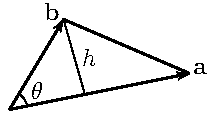
\includegraphics{sec_1_2_triangle.pdf}
\end{center}
}%
Thus the area of the triangle is  $\half|\va|\,|\vb|\,\sin\theta$.
By property 2 of the cross product in Theorem \eref{CLP200}{thm:crossPppties}
of the CLP-3 text,
 $|\va\times\vb|=|\va|\,|\vb|\,\sin\theta$. So
\begin{align*}
\text{area} &= \half|\va\times\vb|
=\half|\llt 1,2,3\rgt\times\llt 3,2,1\rgt| \\
&=\half | \hi\,(2-6)-\hj\,(1-9) +\hk\,(2-6)| \\
&=\half\sqrt{16+64+16} \\
&=2\sqrt{6} 
\end{align*}
\end{solution}

%%%%%%%%%%%%%%%%%%%%%%%%%%%%%%%%
\begin{question}[M200 2003D] %8
 A particle $P$ of unit mass whose position in space at time
$t$ is $\vr(t)$ has angular momentum $L(t)=\vr(t)\times\vr'(t)$.
If $\vr''(t)=\rho(t)\vr(t)$ for a scalar function $\rho$, show that
$L$ is constant, i.e. does not change with time. Here $'$ denotes 
$\diff{}{t}$.
\end{question}

\begin{hint}
Evaluate $\diff{L}{t}$ by differentiating $\vr(t)\times\vr'(t)$.
\end{hint}

\begin{answer}
See the solution.
\end{answer}

\begin{solution}
The derivative of $L$ is
\begin{align*}
\diff{L}{t}=\diff{}{t}\big(\vr(t)\times\vr'(t)\big)
=\vr'(t)\times\vr'(t)+\vr(t)\times\vr''(t)
=\vr'(t)\times\vr'(t)+\vr(t)\times\big(\rho(t)\vr(t)\big)
\end{align*}
Both terms vanish because the cross product of any two parallel vectors
is zero. So $\diff{L}{t}=0$ and $L(t)$ is independent of $t$. 
\end{solution}



%%%%%%%%%%%%%%%%%%
\subsection*{\Application}
%%%%%%%%%%%%%%%%%%

\begin{question}
Show that the diagonals of a parallelogram bisect each other.
\end{question}

%\begin{hint}
%\end{hint}

\begin{answer}
See the solution.
\end{answer}

\begin{solution}
The parallelogram determined by the vectors $\va$ and $\vb$
has vertices $\vZero,\ \va,\ \vb$ and $\va+\vb$.
As $t$ varies from $0$ to $1$, $t(\va+\vb)$ traverses the
diagonal from $\vZero$ to $\va+\vb$.
As $s$ varies from $0$ to $1$, $\va+s(\vb-\va)$ traverses the
diagonal from $\va$ to $\vb$. These two straight lines meet
when $s$ and $t$ are such that
\begin{equation*}
t(\va+\vb)=\va+s(\vb-\va)
\end{equation*}
or
\begin{equation*}
(t+s-1)\va=(s-t)\vb
\end{equation*}
Assuming that $\va$ and $\vb$ are not parallel (i.e. the parallelogram
has not degenerated to a line segment), this is the case only
when $t+s-1=0$ and $s-t=0$. That is, $s=t=\half$. So the two lines
meet at their midpoints.
\end{solution}

%%%%%%%%%%%%%%%%%%%%%%%%%%%%%%%%
\begin{question}
Consider a cube such that each side has length $s$. Name,
in order, the four vertices on the bottom of the cube $A, B, C, D$ and the
corresponding four vertices on the top of the cube $A', B', C', D'$.
\begin{enumerate}[(a)]
\item 
Show that all edges of the tetrahedron $A'C'BD$ have the same length.
\item
Let $E$ be the center of the cube. Find the angle between $EA$ and $EC$.
\end{enumerate}
\end{question}

%\begin{hint}
%
%\end{hint}

\begin{answer}
(a) All $6$ edges have length $\sqrt{2}s$.\qquad
(b) $109.5^\circ$
\end{answer}

\begin{solution}
We may choose our coordinate axes so that $A=(0,0,0)$,  $B=(s,0,0)$,
$C=(s,s,0)$, $D=(0,s,0)$ and $A'=(0,0,s)$, $B'=(s,0,s)$,
$C'=(s,s,s)$, $D'=(0,s,s)$.

(a) Then
\begin{alignat*}{5}
|A'C'|&=\big|\llt s,s,s\rgt -\llt 0,0,s\rgt \big|
      &&=\big|\llt s,s,0\rgt \big|&=\sqrt{2}\,s\\
|A'B|&=\big|\llt s,0,0\rgt -\llt 0,0,s\rgt \big|
     &&=\big|\llt s,0,-s\rgt \big|&=\sqrt{2}\,s\\
|A'D|&=\big|\llt 0,s,0\rgt -\llt 0,0,s\rgt \big|
     &&=\big|\llt 0,s,-s\rgt \big|&=\sqrt{2}\,s\\
|C'B|&=\big|\llt s,0,0\rgt -\llt s,s,s\rgt \big|
     &&=\big|\llt 0,-s,-s\rgt \big|&=\sqrt{2}\,s\\
|C'D|&=\big|\llt 0,s,0\rgt -\llt s,s,s\rgt \big|
     &&=\big|\llt -s,0,-s\rgt \big|&=\sqrt{2}\,s\\
|BD|&=\big|\llt 0,s,0\rgt -\llt s,0,0\rgt \big|
    &&=\big|\llt -s,s,0\rgt \big|&=\sqrt{2}\,s
\end{alignat*}

(b) $E=\half(s,s,s)$ so that $EA=\llt 0,0,0\rgt -\half\llt s,s,s\rgt 
      =-\half\llt s,s,s\rgt $ and 
$EC=\llt s,s,0\rgt -\half\llt s,s,s\rgt =\half\llt s,s,-s\rgt $.
$$
\cos\theta =\frac{-\llt s,s,s\rgt \cdot\llt s,s,-s\rgt}
                 {|\llt s,s,s\rgt |\,|\llt s,s,-s\rgt |}
        =\frac{-s^2}{3s^2}
        =-\frac{1}{3}
\qquad \implies\quad \theta=109.5^\circ
$$
\end{solution}

%%%%%%%%%%%%%%%%%%%%%%%%%%%%%%%%
\begin{question}
Find the angle between the diagonal of a cube and the diagonal
of one of its faces.
\end{question}

%\begin{hint}
%
%\end{hint}

\begin{answer}
$35.26^\circ$ or $90^\circ$ or $144.74^\circ$
\end{answer}

\begin{solution}
Suppose that the cube has height, length and width $s$.
We may choose our coordinate axes so that the vertices
of the cube are at $(0,0,0)$, $(s,0,0)$, $(0,s,0)$, $(0,0,s)$, 
$(s,s,0)$, $(0,s,s)$, $(s,0,s)$ and $(s,s,s)$. 

We'll start with a couple of examples. The diagonal from $(0,0,0)$
to $(s,s,s)$ is $\llt s,s,s\rgt$. One face of the cube has vertices $(0,0,0)$,
$(s,0,0)$, $(0,s,0)$ and $(s,s,0)$. One diagonal of this face runs from
$(0,0,0)$ to $(s,s,0)$ and hence is $\llt s,s,0\rgt$. The angle between 
$\llt s,s,s\rgt$ and $\llt s,s,0\rgt$ is
\begin{align*}
\cos^{-1}\left(\frac{\llt s,s,s\rgt\cdot\llt s,s,0\rgt}
                    {|\llt s,s,s\rgt|\,|\llt s,s,0\rgt|}\right)
=\cos^{-1}\left(\frac{2s^2}{\sqrt{3}s\,\sqrt{2}s}\right)
=\cos^{-1}\left(\frac{2}{\sqrt{6}}\right)\approx 35.26^\circ
\end{align*}
A second diagonal for the face with vertices  $(0,0,0)$,
$(s,0,0)$, $(0,s,0)$ and $(s,s,0)$ is that running from
$(s,0,0)$ to $(0,s,0)$. This diagonal is $\llt -s,s,0\rgt$. The angle between 
$\llt s,s,s\rgt$ and $\llt -s,s,0\rgt$ is
\begin{align*}
\cos^{-1}\left(\frac{\llt s,s,s\rgt\cdot\llt -s,s,0\rgt}
               {|\llt s,s,s\rgt|\,|\llt -s,s,0\rgt|}\right)
=\cos^{-1}\left(\frac{0}{\sqrt{3}s\,\sqrt{2}s}\right)
=\cos^{-1}(0)=90^\circ
\end{align*}

Now we'll consider the general case.
Note that every component of every vertex of the cube is either $0$ or
$s$. In general, two vertices of the cube are at
opposite ends of a diagonal of the cube if all three components of the
two vertices are different. For example, if one end of the diagonal is
$(s,0,s)$, the other end is $(0,s,0)$. The diagonals of the cube are all 
of the form $\llt \pm s,\pm s,\pm s\rgt$. All of these diagonals are of length $\sqrt{3}s$.
Two vertices are on the same face of the cube if one of their components
agree. They are on opposite ends of a diagonal for the face if their other
two components differ. For example $(0,s,s)$ and $(s,0,s)$ are both on
the face with $z=s$.  Because the $x$ components $0,\ s$ are different
and the $y$ components $s,\ 0$ are different, $(0,s,s)$ and $(s,0,s)$
are the ends of a diagonal of the face with $z=s$. The diagonals of the
faces with $z=0$ or $z=s$ are $\llt \pm s,\pm s,0\rgt$. The diagonals of the
faces with $y=0$ or $y=s$ are $\llt \pm s,0, \pm s\rgt$. The diagonals of the
faces with $x=0$ or $x=s$ are $\llt 0,\pm s,\pm s\rgt$. All of these diagonals
have length $\sqrt{2}s$. The dot product of one the cube diagonals
$\llt \pm s,\pm s,\pm s\rgt$ with one of the face diagonals  $\llt \pm s,\pm s,0\rgt$,
 $\llt \pm s,0, \pm s\rgt$, $\llt 0,\pm s,\pm s\rgt$ is of the form $\pm s^2\pm s^2+0$
and hence must be either $2s^2$ or $0$ or $-2s^2$. In general, the angle
between a cube diagonal and a face diagonal is
\begin{align*}
\cos^{-1}\left(\frac{\text{$2s^2$ or 0 or $-2s^2$}}{\sqrt{3}s\,\sqrt{2}s}\right)
=\cos^{-1}\left(\frac{\text{$2$ or $0$ or $-2$}}{\sqrt{6}}\right)\approx 
\text{$35.26^\circ$ or $90^\circ$ or $144.74^\circ$}. 
\end{align*}
\end{solution}


%%%%%%%%%%%%%%%%%%%%%%%%%%%%%%%%%%%%
\begin{question}
Consider a skier who is sliding without friction on the
hill $y=h(x)$ in a two dimensional world. The skier is subject to two
forces. One is gravity. The other acts perpendicularly to the hill. The second force automatically adjusts its magnitude so as to prevent the skier from burrowing into the hill. Suppose that the skier became
airborne at some $(x_0,y_0)$ with $y_0=h(x_0)$. How fast was the skier going? 

\end{question}

%\begin{hint}
%\end{hint}

\begin{answer}
$\sqrt{1+h'\big(x_0\big)^2}\sqrt{-g/h''\big(x_0\big)}$
\end{answer}

\begin{solution}
Denote by $\big(x(t),y(t)\big)$ the position of the skier at time $t$. As long as the skier remains on the surface of the hill
\begin{align*}
y(t)&=h\big(x(t)\big)   \\
\implies y'(t)&=h'\big(x(t)\big)\,x'(t)  \\
\implies y''(t)&=h''\big(x(t)\big)\, x'(t)^2+h'\big(x(t)\big)\,x''(t)
\end{align*}
So the velocity and acceleration vectors of the skier are
\begin{align*}
\vv(t)&=\llt 1,h'\big(x(t)\big)\rgt x'(t) \\
\va(t)&=\llt 1,h'\big(x(t)\big)\rgt x''(t)
+\llt 0,h''\big(x(t)\big)\rgt x'(t)^2
\end{align*}
The skier is subject to two forces. One is gravity. The other
acts perpendicularly to the hill and has a magnitude such that the skier
remains on the surface of the hill. From the velocity vector of the
skier (which remain tangential to the hill as long as the skier
remains of the surface of the hill),we see that one vector normal to
the hill at $\big(x(t),y(t)\big)$ is 
$$
\vn(t)=\llt-h'\big(x(t)\big),1\rgt
$$
This vector is not a unit  vector, but that's ok. By Newton's law
of motion
\begin{equation*}
m\va=-mg\,\hj+p(t)\,\vn(t)
\end{equation*}
for some function $p(t)$.
Dot both sides of this equation with $\vn(t)$.
\begin{equation*}
m\va(t)\cdot\vn(t)=-mg\hj\cdot\vn(t)+p(t)|\vn(t)|^2
\end{equation*}
Substituting in
\begin{align*}
mh''\big(x(t)\big)\,x'(t)^2&=-mg+p(t)\left[1+h'\big(x(t)\big)^2\right] \\
\implies p(t)\left[1+h'\big(x(t)\big)^2\right]
&=m\Big(g+h''\big(x(t)\big)\,x'(t)^2\Big)
\end{align*}
As long as $p(t)\ge 0$, the hill is pushing up in order to keep the skier
on the surface. When $p(t)$ becomes negative, the hill has to pull on the
skier in order to keep her on the surface. But the hill can't pull, 
so the skier becomes airborne instead. This happens when
\begin{equation*}
g+h''\big(x(t)\big)x'(t)^2=0
\end{equation*}
That is when $x'(t)=\sqrt{-g/h''\big(x(t)\big)}$. At this time $x(t)=x_0$, $y(t)=y_0$ and the speed of the skier is 
\begin{equation*}
\sqrt{x'(t)^2+y'(t)^2}
=\sqrt{1+h'\big(x_0\big)^2}\sqrt{-g/h''\big(x_0\big)}
\end{equation*}
\end{solution}


%%%%%%%%%%%%%%%%%%%%%%%%%%%%%%%%%%%%
\begin{question}
A marble is placed on the plane $ax+by+cz=d$. The coordinate
system has been chosen so that the positive $z$--axis points straight up.
The coefficient $c$ is nonzero and the coefficients $a$ and $b$ are not
both zero.
In which direction does the marble roll? 
Why were the conditions ``$c\ne 0$'' and ``$a,b$ not both zero'' imposed?
\end{question}

%\begin{hint}
%\end{hint}

\begin{answer}
The marble rolls in the directionn$\llt ac,bc,-a^2-b^2\rgt$.
If $c=0$, the plane is vertical. In this case, the marble
doesn't roll -- it falls straight down. If $a=b=0$, the plane is horizontal.
 In this case, the marble doesn't roll --- it remains stationary.
\end{answer}

\begin{solution}
The marble is subject to two forces. The first, gravity, is
$-mg\,\hk$ with $m$ being the mass of the marble. The second is the normal
force imposed by the plane. This forces acts in a direction perpendicular
to the plane. One vector normal to the plane is $a\,\hi+b\,\hj+c\,\hk$. 
So the force due to the plane is $T\llt a,b,c\rgt$ with $T$ determined  by the
property that the net force perpendicular to the plane must be exactly
zero, so that the marble remains on the plane, neither digging into nor
flying off of it. The projection of the gravitational force onto the normal
vector $\llt a,b,c\rgt$ is
\begin{equation*}
\frac{-mg\llt 0,0,1\rgt\cdot\llt a,b,c\rgt}{|\llt a,b,c\rgt|^2}\llt a,b,c\rgt
=\frac{-mgc}{a^2+b^2+c^2}\llt a,b,c\rgt
\end{equation*}
The condition that determines $T$ is thus
\begin{equation*}
T\llt a,b,c\rgt+\frac{-mgc}{a^2+b^2+c^2}\llt a,b,c\rgt =0
\implies T=\frac{mgc}{a^2+b^2+c^2}
\end{equation*}
The total force on the marble is then (ignoring friction -- which will
have no effect on the direction of motion)
\begin{align*}
T\llt a,b,c\rgt-mg\llt 0,0,1\rgt&=\frac{mgc}{a^2+b^2+c^2}\llt a,b,c\rgt-mg\llt 0,0,1\rgt\cr
&=mg\frac{c\llt a,b,c\rgt-\llt 0,0,a^2+b^2+c^2\rgt}{a^2+b^2+c^2}\cr
&=mg\frac{\llt ac,bc,-a^2-b^2\rgt}{a^2+b^2+c^2}\cr
\end{align*}
The direction of motion $\llt ac,bc,-a^2-b^2\rgt$. If you want to turn
this into a unit vector, just divide by $\sqrt{(a^2+b^2)(a^2+b^2+c^2)}$.
Note that the direction vector in perpendicular $\llt a,b,c\rgt$ and hence is parallel
to the plane. If $c=0$, the plane is vertical. In this case, the marble
doesn't roll -- it falls straight down. If $a=b=0$, the plane is horizontal.
 In this case, the marble doesn't roll --- it remains stationary.
\end{solution}

%%%%%%%%%%%%%%%%%%%%%%%%%%%%%%%%%%%%
\begin{question}
Show that $\va\cdot(\vb\times\vc)
                         =(\va\times\vb)\cdot\vc$.
\end{question}

%\begin{hint}
%\end{hint}

\begin{answer}
See the solution.
\end{answer}

\begin{solution} By definition, the left and right hand sides are
\begin{align}
\va\cdot(\vb\times\vc)
&=\llt a_1,a_2,a_3\rgt \cdot\llt b_2c_3-b_3c_2, b_3c_1-b_1c_3, b_1c_2-b_2c_1\rgt \notag\\
&=a_1b_2c_3 - a_1b_3c_2 + a_2b_3c_1 - a_2b_1c_3 + a_3b_1c_2 - a_3b_2c_1
\tag{lhs}\\
\notag\\
(\va\times\vb)\cdot\vc
&=\llt a_2b_3-a_3b_2, a_3b_1-a_1b_3, a_1b_2-a_2b_1\rgt \cdot\llt c_1,c_2,c_3\rgt \notag\\
&=a_2b_3c_1 - a_3b_2c_1 + a_3b_1c_2 - a_1b_3c_2 + a_1b_2c_3 - a_2b_1c_3
\tag{rhs}
\end{align}
(lhs) and (rhs) are the same.
\end{solution}


%%%%%%%%%%%%%%%%%%%%%%%%%%%%%%%%%%%%
\begin{question}
Show that $\va\times(\vb\times\vc)
=(\va\cdot\vc)\vb-(\va\cdot\vb)\vc$.
\end{question}

%\begin{hint}
%\end{hint}

\begin{answer}
See the solution.
\end{answer}

\begin{solution}
By definition, 
\begin{align*}
\vb\times\vc
\ =\ &(b_2c_3-b_3c_2)\hi-(b_1c_3-b_3c_1)\hj
    +(b_1c_2-b_2c_1)\hk \\
\intertext{so that the left and right hand sides are}
\va\times(\vb\times\vc)
\ =\ &\det\left[\begin{matrix}\hi&\hj &\hk\\
                     a_1&a_2&a_3\\
            b_2c_3-b_3c_2&-b_1c_3+b_3c_1&b_1c_2-b_2c_1\end{matrix}\right]\\
\ =\ &\hi\,[a_2(b_1c_2-b_2c_1)-a_3(-b_1c_3+b_3c_1)]\\
{-}&\hj\,[a_1(b_1c_2-b_2c_1)-a_3(b_2c_3-b_3c_2)]\\
{+}&\hk\,[a_1(-b_1c_3+b_3c_1)-a_2(b_2c_3-b_3c_2)]&{\rm (lhs)}\\
\noalign{\vskip0.05in}
(\va\cdot\vc)\vb-(\va\cdot\vb)\vc
\ =\ &(a_1c_1+a_2c_2+a_3c_3)(b_1\hi+b_2\hj+b_3\hk)
-(a_1b_1+a_2b_2+a_3b_3)(c_1\hi+c_2\hj+c_3\hk)\\
{=}\ &
\hi\,[a_1b_1c_1+a_2b_1c_2+a_3b_1c_3-a_1b_1c_1-a_2b_2c_1-a_3b_3c_1]
\\
{+}&\hj\,[a_1b_2c_1+a_2b_2c_2+a_3b_2c_3-a_1b_1c_2-a_2b_2c_2-a_3b_3c_2]
\\
{+}&\hk\,[a_1b_3c_1+a_2b_3c_2+a_3b_3c_3-a_1b_1c_3-a_2b_2c_3-a_3b_3c_3]\cr
{=}\ &
\hi\,[a_2b_1c_2+a_3b_1c_3-a_2b_2c_1-a_3b_3c_1]
\\
{+}&\hj\,[a_1b_2c_1+a_3b_2c_3-a_1b_1c_2-a_3b_3c_2]
\\
{+}&\hk\,[a_1b_3c_1+a_2b_3c_2-a_1b_1c_3-a_2b_2c_3]
&{\rm (rhs)}
\end{align*}
(lhs) and (rhs) are the same.
\end{solution}


%%%%%%%%%%%%%%%%%%%%%%%%%%%%%%%%%%%%
\begin{question}
Derive a formula for $(\va\times\vb)\cdot(\vc\times\vd)$
that involves dot but not cross products.
\end{question}

%\begin{hint}
%\end{hint}

\begin{answer}
$(\va\times\vb)\cdot(\vc\times\vd)=
(\va\cdot\vc)(\vb\cdot\vd)
-(\va\cdot\vd)(\vb\cdot\vc)$
\end{answer}

\begin{solution}
By properties 9 and 10 of Theorem \eref{CLP200}{thm:crossPppties} in the CLP-3 
text,
\begin{align*}
(\va\times\vb)\cdot(\vc\times\vd)
&=\va\cdot[\vb\times(\vc\times\vd)]
\hskip.5in&\text{(by property 9 with $\vc\rightarrow (\vc\times\vd)$)} \\
&=\va\cdot[(\vb\cdot\vd)\vc-(\vb\cdot\vc)\vd]
\hskip.25in&\text{(by property 10)}\cr
&=(\va\cdot\vc)(\vb\cdot\vd)
-(\va\cdot\vd)(\vb\cdot\vc)
\end{align*}
So
\begin{equation*}
(\va\times\vb)\cdot(\vc\times\vd)=
(\va\cdot\vc)(\vb\cdot\vd)
-(\va\cdot\vd)(\vb\cdot\vc)
\end{equation*}
\end{solution}


%%%%%%%%%%%%%%%%%%%%%%%%%%%%%%%%%%%%
\begin{question}
A prism has the six vertices
\begin{alignat*}{3}
A&=(1,0,0)\qquad   &  A'&=(5,0,1) \\
B&=(0,3,0)   &  B'&=(4,3,1) \\
C&=(0,0,4)   &  C'&=(4,0,5) 
\end{alignat*}
\begin{enumerate}[(a)]
\item
  Verify that three of the faces are parallelograms.
  Are they rectangular?
\item
  Find the length of $AA'$.
\item
  Find the area of the triangle $ABC$.
\item
   Find the volume of the prism.
\end{enumerate}
\end{question}

%\begin{hint}
%\end{hint}

\begin{answer}
(a)
$AA'B'B$ is a parallelogram, but not a rectangle.\\
$AA'C'C$ is a rectangle.\\
$BB'C'C$ is a parallelogram, but not a rectangle.

(b) $\sqrt{17}$ \qquad
(c) $\frac{13}{2}$\qquad
(d) $\frac{51}{2}$


\end{answer}

\begin{solution}
(a) $AA'=\llt 4,0,1\rgt $ and $BB'=\llt 4,0,1\rgt $ are opposite sides
of the quadrilateral $AA'B'B$. They have the same length 
and direction. The same is true for $AB=\llt -1,3,0\rgt $ and 
$A'B'=\llt -1,3,0\rgt $. So $AA'B'B$ is a parallelogram. Because, 
$AA'\cdot AB=\llt 4,0,1\rgt \cdot\llt -1,3,0\rgt =-4\ne 0$, 
the neighbouring edges of $AA'B'B$ are not perpendicular and so $AA'B'B$ 
is \emph{not} a rectangle.

Similarly, the quadilateral $ACC'A'$ has opposing sides
$AA'=\llt 4,0,1\rgt =CC'=\llt 4,0,1\rgt $ and 
$AC=\llt -1,0,4\rgt =A'C'=\llt -1,0,4\rgt $ and so is
a parallelogram. Because $AA'\cdot AC=\llt 4,0,1\rgt \cdot\llt -1,0,4\rgt = 0$, the neighbouring edges of $ACC'A'$ are perpendicular, so
$ACC'A'$ \emph{is} a rectangle.

Finally, the quadilateral $BCC'B'$ has opposing sides
$BB'=\llt 4,0,1\rgt =CC'=\llt 4,0,1\rgt $ and 
$BC=\llt 0,-3,4\rgt =B'C'=\llt 0,-3,4\rgt $ and so is
a parallelogram. Because $BB'\cdot BC=\llt 4,0,1\rgt \cdot\llt 0,-3,4\rgt 
= 4\ne 0$, the neighbouring edges of $BCC'B'$ are not perpendicular, so 
$BCC'B'$ is \emph{not} a rectangle.

(b) The length of $AA'$ is $|\llt 4,0,1\rgt |=\sqrt{16+1}=\sqrt{17}$.

(c) The area of a triangle is one half its base times its height. 
That is, one half times $|AB|$ times $|AC|\sin\theta$, where 
$\theta$ is the angle between $AB$ and $AC$. This is precisely 
$\half |AB\times AC|=\half|\llt -1,3,0\rgt \times\llt -1,0,4\rgt | 
=\half |\llt 12,4,3\rgt|=\frac{13}{2}$.

(d) The volume of the prism is the area of its base $ABC$,
 times its height, which is the length of $AA'$ times the cosine of the
angle between $AA'$ and the normal to $ABC$. This coincides with
$\half \llt 12,4,3\rgt \cdot\llt 4,0,1\rgt =\half(48+3)=\frac{51}{2}$, which is 
one half times the length of $\llt 12,4,3\rgt $ (the area of $ABC$) 
times the length of $\llt 4,0,1\rgt $ (the length of $AA'$) times the 
cosine of the angle between $\llt 12,4,3\rgt $ and
$\llt 4,0,1\rgt $ (the angle between the normal to $ABC$ and $AA'$).

\end{solution}

%%%%%%%%%%%%%%%%%%%%%%%%%%%%%%%%%%%%
\begin{question}\label{prb pythagorous}
(Three dimensional Pythagorean Theorem) A solid body in space 
with exactly four vertices is called a tetrahedron. Let $A$, $B$, $C$ and
$D$ be the areas of the four faces of a tetrahedron. Suppose that the
three edges meeting at the vertex opposite the face of area $D$ are 
perpendicular to each other. Show that $D^2=A^2+B^2+C^2$.

\begin{center}
     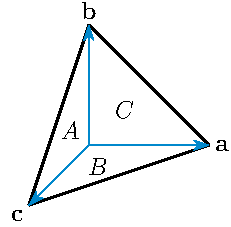
\includegraphics{tetrahedron.pdf}
\end{center}

\end{question}

\begin{hint}
Choose coordinate axes so that the vertex opposite
the face of area $D$ is at the origin. Denote  by $\va$, $\vb$ and
$\vc$ the vertices opposite the sides of area $A$, $B$ and $C$ respectively.
Express $A$, $B$, $C$ and $D$, which are areas of triangles, as one half 
times cross products of vectors built from $\va$, $\vb$ and $\vc$.
\end{hint}

\begin{answer}
See the solution.
\end{answer}

\begin{solution}
Choose our coordinate axes so that the vertex opposite
the face of area $D$ is at the origin. Denote  by $\va$, $\vb$ and
$\vc$ the vertices opposite the sides of area $A$, $B$ and $C$ respectively.
Then the face of area $A$ has edges $\vb$ and $\vc$ so that
$A=\half |\vb\times\vc|$. Similarly $B=\half|\vc\times\va|$ and
$C=\half|\va\times \vb|$. The face of area $D$ is the triangle 
spanned by $\vb-\va$ and $\vc-\va$ so that
\begin{align*}
D&=\half|(\vb-\va)\times(\vc-\va)|\cr
&=\half|\vb\times \vc-\va\times\vc-\vb\times\va|\\
&=\half|\vb\times \vc+\vc\times\va+\va\times\vb|
\end{align*} 
By hypothesis, the vectors $\va$, $\vb$ and $\vc$ are all perpendicular
to each other. Consequently the vectors $\vb\times \vc$ (which is
a scalar times $\va$), $\vc\times\va$ (which is a scalar times
$\vb$) and $\va\times\vb$ (which is a scalar times $\vc$)
are also mutually perpendicular. So, when we multiply out
\begin{equation*}
D^2=\frac{1}{4}\big[\vb\times \vc+\vc\times\va+\va\times\vb\big]\cdot\big[\vb\times \vc+\vc\times\va+\va\times\vb\big]
\end{equation*}
all the cross terms vanish, leaving
\begin{equation*}
D^2=\frac{1}{4}\big[(\vb\times \vc)\cdot(\vb\times \vc)
+(\vc\times\va)\cdot(\vc\times\va)
+(\va\times\vb)\cdot(\va\times\vb)\big]=A^2+B^2+C^2
\end{equation*}
\end{solution}

%%%%%%%%%%%%%%%%%%%%%%%%%%%%%%%%%%%%
\begin{question}
(Three dimensional law of cosines)  Let $A$, $B$, $C$ and
$D$ be the areas of the four faces of a tetrahedron. Let 
$\al$ be the angle between the faces with areas $B$ and $C$, 
$\be$ be the angle between the faces with areas $A$ and $C$ and 
$\ga$ be the angle between the faces with areas $A$ and $B$. 
(By definition, the angle between two faces is the angle between the normal vectors to the faces.)
 Show that 
\begin{equation*}
D^2=A^2+B^2+C^2-2BC\cos\al-2AC\cos\be-2AB\cos\ga
\end{equation*}
\end{question}

\begin{hint}
  Do problem \ref{prb pythagorous} first.
\end{hint}

\begin{answer}
See the solution.
\end{answer}

\begin{solution}
As in problem \ref{prb pythagorous},
\begin{equation*}
D^2=\frac{1}{4}
  \big[\vb\times \vc+\vc\times\va+\va\times\vb\big]\cdot
  \big[\vb\times \vc+\vc\times\va+\va\times\vb\big]
\end{equation*}
But now $(\vb\times \vc)\cdot(\va\times\vc)$, instead of vanishing,
is $|\vb\times \vc|=2A$ times $|\va\times\vc|=2B$ times
the cosine of the angle between $\vb\times \vc$ (which is perpendicular
to the face of area $A$) and $\va\times\vc$ (which is perpendicular
to the face of area $B$). That is
\begin{align*}
(\vb\times \vc)\cdot(\va\times\vc)&=4 AB\cos \ga\\
(\va\times \vb)\cdot(\vc\times\vb)&=4 AC\cos \be\\
(\vb\times \va)\cdot(\vc\times\va)&=4 BC\cos \al
\end{align*}
(If you're worried about the signs, that is, if you are worried about 
why $(\vb\times \vc)\cdot(\va\times\vc)=4 AB\cos \ga$
rather than $(\vb\times \vc)\cdot(\vc\times\va)=4 AB\cos \ga$,
note  that when $\va\approx\vb$, 
$(\vb\times \vc)\cdot(\va\times\vc)\approx|\vb\times\vc|^2$ is positive and 
$(\vb\times \vc)\cdot(\vc\times\va) \approx -|\vb\times\vc|^2$ is negative.) Now, expanding out
\begin{align*}
D^2\ =\ &\frac{1}{4}
   \big[\vb\times \vc+\vc\times\va+\va\times\vb\big]\cdot
   \big[\vb\times \vc+\vc\times\va+\va\times\vb\big] \\
=\ &\frac{1}{4}\big[(\vb\times \vc)\cdot(\vb\times \vc)
     +(\vc\times\va)\cdot(\vc\times\va)
     +(\va\times\vb)\cdot(\va\times\vb) \\
&+2(\vb\times \vc)\cdot(\vc\times \va)
 +2(\vb\times \vc)\cdot(\va\times \vb)
 +2(\vc\times \va)\cdot(\va\times \vb)\big] \\
=\ &A^2+B^2+C^2-2 AB\cos \ga-2 AC\cos \be-2 BC\cos \al
\end{align*}
\end{solution}





%\setcounter{section}{3}
\section{Equations of Lines in 2d}
%\documentclass[12pt]{article}

\questionheader{ex:s1.3}

%%%%%%%%%%%%%%%%%%
\subsection*{\Conceptual}
%%%%%%%%%%%%%%%%%%

%%%%%%%%%%%%%%%%%%%
\begin{question}\label{prob1.3_signs}
A line in $\mathbb R^2$ has direction $\mathbf d$ and passes through point $\mathbf c$.

Which of the following gives its parametric equation: $\llt x,y\rgt =\mathbf c + t\mathbf d $, or $\llt x,y\rgt =\mathbf c - t\mathbf d $?

\end{question}
\begin{hint}
What, exactly, is $t$?
\end{hint}
\begin{answer}
Both!
\end{answer}
\begin{solution}
Since $t$ can be any real number, these equation describe the same line. They're both valid. For example, the point given by the first parametric 
equation with $t=7$, namely $\mathbf c + 7\mathbf d $, 
is exactly the same as the point given by the second  parametric equation 
with $t=-7$, namely $\mathbf c -(-7)\mathbf d $.
\end{solution}
%%%%%%%%%%%%%%%%%%%

%%%%%%%%%%%%%%%%%%%
\begin{question}
A line in $\mathbb R^2$ has direction $\mathbf d$ and passes through point $\mathbf c$.

Which of the following gives its parametric equation: $\llt x,y\rgt =\mathbf c + t\mathbf d $, or $\llt x,y\rgt =-\mathbf c +t \mathbf d$?

\end{question}
\begin{hint}
What, exactly, is $\mathbf c$?
\end{hint}
\begin{answer}
Generally, only the first.
\end{answer}
\begin{solution}
In contrast to Question~\ref{prob1.3_signs}, the sign on $\mathbf c$ does generally matter. $\mathbf c$ is required to be a point on the line, but except in particular circumstances, there's no reason to believe that 
$-\mathbf c =-\mathbf c +t\mathbf d\big|_{t=0}$ is a point on the line. 
Indeed $-\mathbf c$ is on the line if and only if there is a $t$ with
$\mathbf c + t\mathbf d = -\mathbf c$, i.e. $t\mathbf d = -2\mathbf c$.
That is the case if and only if $\mathbf d$ is parallel to $\mathbf c$.
So, only the first equation is correct in general.
\end{solution}
%%%%%%%%%%%%%%%%%%%

%%%%%%%%%%%%%%%%%%%
%%%%%%%%%%%%%%%%%%%
\begin{question} Two points determine a line. Verify that the equations 

\[\llt x-1,y-9\rgt=t\llt 8,4\rgt\]
and
\[\llt x-9,y-13\rgt=t\llt 1,\tfrac12\rgt\]

describe the same line by finding two different points that lie on both lines.
\end{question}
\begin{hint}
Set $t=0$ in both equation to get two different points with integer coordinates; show that these two points are on both lines.
\end{hint}
\begin{answer}
Since both lines pass through $(1,9)$ and $(9,13)$, the lines are identical.
\end{answer}
\begin{solution}
Here is one answer of many. 

Setting $t=0$ in the first equation shows that
$(1,9)$ is on the first line. To see that $(1,9)$ is also on the second line,
we substitute $x=1$, $y=9$ into the second equation to give
\begin{equation*}
\llt 1-9,9-13\rgt=t\llt 1,\tfrac12\rgt\qquad \text{or}\qquad
\llt -8,-4\rgt=t\llt 1,\tfrac12\rgt
\end{equation*}
This equation is satisfied when $t=-8$. So $(1,9)$ is on both lines.

Setting $t=0$ in the second equation shows that
$(9,13)$ is on the second line. To see that $(9,13)$ is also on the first line,
we substitute $x=9$, $y=13$ into the first equation to give
\begin{equation*}
\llt 9-1,13-9\rgt=t\llt 8,4\rgt\qquad \text{or}\qquad
\llt 8,4\rgt=t\llt 8,4\rgt
\end{equation*}
This equation is satisfied when $t=1$. So $(9,13)$ is on both lines.

Since both lines pass through $(1,9)$ and $(9,13)$, the lines are identical.
\end{solution}
%%%%%%%%%%%%%%%%%%%
\begin{question}
A line in $\mathbb R^2$ has parametric equations
\[\begin{array}{lcl}
x-3&=&9t\\
y-5&=&7t
\end{array}\]
There are many different ways to write the parametric equations of this line. If we rewrite the equations as
\[\begin{array}{lcl}
x-x_0&=&d_xt\\
y-y_0&=&d_yt
\end{array}\]
what are all possible values of $\llt x_0,y_0\rgt$ and $\llt d_x,d_y\rgt$?
\end{question}
\begin{hint}
A line is specified by two things: one point on the line, and a vector parallel to the direction of the line.
\end{hint}
\begin{answer}
$\llt d_x,d_y\rgt$ can be any nonzero scalar multiple of $\llt 9,7\rgt$, and $\llt x_0,y_0\rgt$ can be any point on the line, i.e. any pair that satisfies $7x_0+24=9y_0$.
\end{answer}
\begin{solution}
$\llt d_x,d_y\rgt$ is the direction of the line, so it can be any \textbf{non-zero} scalar multiple of $\llt 9,7\rgt$.

$\llt x_0,y_0\rgt$ can be any point on the line. Describing these is the same as describing the line itself. We're trying to find all 
doubles $\llt x_0,y_0\rgt$  that obey
\begin{align*}
\begin{cases}
x_0-3&=9t\\
y_0-5&=7t
\end{cases}
\end{align*}
for some real number $t$. That is,
\begin{align*}
t=\frac{x_0-3}{9}&=\frac{y_0-5}{7}\\
7(x_0-3)&=9(y_0-5)\\
7x_0+24&=9y_0
\end{align*}

Any of these steps could specify the possible values of $\llt x_0,y_0\rgt$. 
Say, they can be any pair satisfying $7x_0+24=9y_0$.
\end{solution}
%%%%%%%%%%%%%%%%%%%




%%%%%%%%%%%%%%%%%%
\subsection*{\Procedural}
%%%%%%%%%%%%%%%%%%

%%%%%%%%%%%%%%%%%%%%%%%%%%%%%%%%%%%%
\begin{question}
Find the vector parametric, scalar parametric
 and symmetric equations for the line
containing the given point and with the given direction.
\begin{enumerate}[(a)]
\item point $(1,2)$, direction $\llt 3,2\rgt $
\item point $(5,4)$, direction $\llt 2,-1\rgt $
\item point $(-1,3)$, direction $\llt -1,2\rgt $
\end{enumerate}
\end{question}

\begin{hint}
Remember that the parametric equation of a line with direction $\mathbf d$, passing through point $\mathbf c$, is $\llt x,y\rgt =\mathbf c + t\mathbf d $.
\end{hint}

\begin{answer}
(a) $\llt x,y\rgt=\llt 1,2\rgt+t\llt 3,2\rgt $,\ \ \ 
    $x=1+3t,\ y=2+2t$,\ \ \ 
    $\frac{x-1}{3}=\frac{y-2}{2}$

(b) $\llt x,y\rgt=\llt 5,4\rgt+t\llt 2,-1\rgt $,\ \ \ 
    $x=5+2t,\ y=4-t$,\ \ \ 
    $\frac{x-5}{2}=\frac{y-4}{-1}$

(c) $\llt x,y\rgt=\llt -1,3\rgt+t\llt -1,2\rgt $,\ \ \ 
    $x=-1-t,\ y=3+2t$,\ \ \ 
    $\frac{x+1}{-1}=\frac{y-3}{2}$
\end{answer}

\begin{solution}
(a)
The vector parametric equation is $\llt x,y\rgt=\llt 1,2\rgt+t\llt 3,2\rgt $.
The scalar parametric equations are $x=1+3t,\ y=2+2t$.
The symmetric equation is $\frac{x-1}{3}=\frac{y-2}{2}$.

(b)
The vector parametric equation is $\llt x,y\rgt=\llt 5,4\rgt+t\llt 2,-1\rgt $.
The scalar parametric equations are $x=5+2t,\ y=4-t$.
The symmetric equation is $\frac{x-5}{2}=\frac{y-4}{-1}$.

(c)
The vector parametric equation is $\llt x,y\rgt=\llt -1,3\rgt+t\llt -1,2\rgt $.
The scalar parametric equations are $x=-1-t,\ y=3+2t$.
The symmetric equation is $\frac{x+1}{-1}=\frac{y-3}{2}$.
\end{solution}

%%%%%%%%%%%%%%%%%%%%%%%%%%%%%%%%%%%%
\begin{question}
Find the vector parametric, scalar parametric
 and symmetric equations for the line
containing the given point and with the given normal.
\begin{enumerate}[(a)]
\item point $(1,2)$, normal $\llt 3,2\rgt $
\item point $(5,4)$, normal $\llt 2,-1\rgt $
\item point $(-1,3)$, normal $\llt -1,2\rgt $
\end{enumerate}
\end{question}

\begin{hint}
Review Equation~\eref{CLP200}{eqn line} in the CLP-3 text.%1.3.3
\end{hint}

\begin{answer}
(a) $\llt x,y\rgt=\llt 1,2\rgt+t\llt -2,3\rgt $,\ \ \ 
    $x=1-2t,\ y=2+3t$,\ \ \ 
    $\frac{x-1}{-2}=\frac{y-2}{3}$

(b) $\llt x,y\rgt=\llt 5,4\rgt+t\llt 1,2\rgt $,\ \ \ 
    $x=5+t,\ y=4+2t$,\ \ \ 
    $x-5=\frac{y-4}{2}$

(c) $\llt x,y\rgt=\llt -1,3\rgt+t\llt 2,1\rgt $,\ \ \ 
    $x=-1+2t,\ y=3+t$,\ \ \ 
    $\frac{x+1}{2}=y-3$
\end{answer}

\begin{solution}
(a) The vector $\llt -2,3\rgt $ is perpendicular to $\llt 3,2\rgt $ (you can
verify this by taking the dot product of the two vectors) and hence is 
a direction vector for the line.
The vector parametric equation is $\llt x,y\rgt=\llt 1,2\rgt+t\llt -2,3\rgt $.
The scalar parametric equations are $x=1-2t,\ y=2+3t$.
The symmetric equation is $\frac{x-1}{-2}=\frac{y-2}{3}$.

(b) The vector $\llt 1,2\rgt $ is perpendicular to $\llt 2,-1\rgt $ 
 and hence is a direction vector for the line.
The vector parametric equation for the line is 
           $\llt x,y\rgt=\llt 5,4\rgt+t\llt 1,2\rgt $.
The scalar parametric equations are $x=5+t,\ y=4+2t$.
The symmetric equation is $x-5=\frac{y-4}{2}$.

(c) The vector $\llt 2,1\rgt $ is perpendicular to $\llt -1,2\rgt $  
and hence is a direction vector for the line.
The vector parametric equation is $\llt x,y\rgt=\llt -1,3\rgt+t\llt 2,1\rgt $.
The scalar parametric equations are the two component equations $x=-1+2t,\ y=3+t$.
The symmetric equation is $\frac{x+1}{2}=y-3$.
\end{solution}



%%%%%%%%%%%%%%%%%%%%%%%%%%%%%%%%%%%%
\begin{question}
Use a projection to find the distance from the point $(-2,3)$
to the line $3x-4y=-4$.
\end{question}

\begin{hint}
Review Example~\eref{CLP200}{eg nearest point} in the CLP-3 text.%1.3.5
\end{hint}

\begin{answer}
$14/5$
\end{answer}

\begin{solution}
$(0,1)$ is one point on the line $3x-4y=-4$. So $\llt-2-0,3-1\rgt
=\llt-2,2\rgt$ is a vector whose tail is on the line and whose 
head is at $(-2,3)$. $\llt 3,-4\rgt$ is a vector perpendicular to the line,
so $\frac{1}{5}\llt 3,-4\rgt$ is a unit vector perpendicular to the line.
The distance from $(-2,3)$ to the line is the length of the projection 
of $\llt-2,2\rgt$ on $\frac{1}{5}\llt 3,-4\rgt$, which is the magnitude of 
$\frac{1}{5}\llt 3,-4\rgt\cdot\llt -2,2\rgt$. So the distance is $14/5$.
\end{solution}



%%%%%%%%%%%%%%%%%%%%%%%%%%%%%%%%%%%%%
\begin{question}
Let $\va$, $\vb$ and $\vc$ be the vertices of a triangle. By definition, 
a median of a triangle is a straight line that passes through a vertex of 
the triangle and through the midpoint of the opposite side.
\begin{enumerate}[(a)]
\item
 Find the parametric equations of the three medians.
\item
 Do the three medians meet at a common point? If so, which point? 
\end{enumerate}
\end{question}

%\begin{hint}
%\end{hint}

\begin{answer}
(a)
\begin{align*}
\vx(t)&=\va+t\big(\half\vb+\half\vc-\va\big)\\
\vx(s)&=\vb+s\big(\half\va+\half\vc-\vb\big)\\
\vx(u)&=\vc+u\big(\half\va+\half\vb-\vc\big)
\end{align*}

(b)
$\frac{1}{3}(\va+\vb+\vc)$
\end{answer}

\begin{solution}
(a) The midpoint of the side opposite $\va$ is
$\half(\vb+\vc)$. The vector joining $\va$ to that midpoint
is $\half\vb+\half\vc-\va$. The vector parametric equation
of the line through $\va$ and $\half(\vb+\vc)$ is
\begin{equation*}
\vx(t)=\va+t\big(\half\vb+\half\vc-\va\big)
\end{equation*}
Similarly, for the other two medians (but using $s$ and $u$ as
parameters, rather than $t$)
\begin{align*}
\vx(s)&=\vb+s\big(\half\va+\half\vc-\vb\big)\\
\vx(u)&=\vc+u\big(\half\va+\half\vb-\vc\big)
\end{align*}

(b) The three medians meet at a common point if there are
values of $s,t$ and $u$ such that
\begin{alignat*}{3}
\va+t\big(\half\vb+\half\vc-\va\big)
&\ =\ \vb+s\big(\half\va+\half\vc-\vb\big)
&&\ =\ \vc+u\big(\half\va+\half\vb-\vc\big)\\
(1-t)\va+\frac{t}{2}\vb+\frac{t}{2}\vc
&\ =\ \frac{s}{2}\va+(1-s)\vb+\frac{s}{2}\vc
&&\ =\ \frac{u}{2}\va+\frac{u}{2}\vb+(1-u)\vc
\end{alignat*}
Assuming that the triangle has not degenerated to a line segment,
this is the case if and only if the coefficients of $\va,\ \vb$ 
and $\vc$ match
\begin{alignat*}{3}
1-t&=\frac{s}{2}&&=\frac{u}{2}\\
\frac{t}{2}&=1-s&&=\frac{u}{2}\\
\frac{t}{2}&=\frac{s}{2}&&=1-u
\end{alignat*}
or
\begin{equation*}
s=t=u,\  1-t=\frac{t}{2}
\implies
s=t=u=\frac{2}{3}
\end{equation*}
The medians meet at $\frac{1}{3}(\va+\vb+\vc)$.
\end{solution}


%%%%%%%%%%%%%%%%%%%
\begin{question}
Let $C$ be the circle of radius 1 centred at $(2,1)$. Find an equation for the line tangent to $C$ at the point $\left(\frac{5}{2},1+\frac{\sqrt3}{2}\right)$.
\end{question}
\begin{hint}
The radius of the circle will serve as a normal vector to the line.
\end{hint}
\begin{answer}
One way of writing the equation is $x+{\sqrt3}y=4+{\sqrt3}$.
\end{answer}
\begin{solution}
A normal vector to the line is the vector with its tail at the centre of $C$, $(2,1)$, and its head at $\left(\frac{5}{2},1+\frac{\sqrt3}{2}\right)$. 
So, we set $\mathbf{n}=\llt \frac{5}{2},1+\frac{\sqrt3}{2} \rgt-\llt 2,1\rgt = 
\llt \frac12, \frac{\sqrt3}{2}\rgt$.


\begin{center}
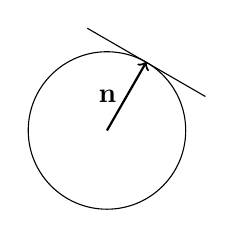
\begin{tikzpicture}
\YEaaxis{.5}{3}{.5}{2}
\draw (2,1) circle (1cm);
%\draw (2,1) node[vertex]{};
\YExcoord{2}{2}
\YEycoord{1}{1}

\draw[thick,->] (2,1)--(2.5,1.87) node[midway, left]{$\mathbf n$};
\draw plot[domain=1.75:3.25](\x,{3.31-\x/1.73});
\end{tikzpicture}
\end{center}

We know one point on the line is $\left(\frac{5}{2},1+\frac{\sqrt3}{2}\right)$, so following Equation~\eref{CLP200}{eqn line}  in the CLP-3 text:
\begin{align*}
n_xx+n_yy&=n_xx_0+n_yy_0\\
\frac12x+\frac{\sqrt3}{2}y&=\frac12\cdot\frac52+\frac{\sqrt3}{2}\cdot\left(1+\frac{\sqrt3}{2}\right)\\
\frac12x+\frac{\sqrt3}{2}y&=2+\frac{\sqrt3}{2}\\
x+{\sqrt3}y&=4+{\sqrt3}\\
\end{align*}
\end{solution}
%%%%%%%%%%%%%%%%%%
%\subsection*{\Application}
%%%%%%%%%%%%%%%%%%
%%%%%%%%%%%%%%%%%%%

%%%%%%%%%%%%%%%%%%%
%%%%%%%%%%%%%%%%%%%
\section{Equations of Planes in 3d}
%\documentclass[12pt]{article}

\questionheader{ex:s1.4}


%%%%%%%%%%%%%%%%%%
\subsection*{\Conceptual}
%%%%%%%%%%%%%%%%%%

%%%%%%%%%%%%%%%%%%%%%%%%%%%%%%%%
\begin{question}
The vector $\hk$ is a normal vector (i.e. is perpendicular) to the plane $z=0$. 
Find another nonzero vector that is normal to $z=0$.
\end{question}

\begin{hint}
You are looking for a vector that is perpendicular to $z=0$ and hence is
parallel to $\hk$. 
\end{hint}

\begin{answer}
Any vector of the form $c\,\hk$ with $c\ne 0$ and $c\ne 1$ works.
Three possible choices are $-\hk$, $2\,\hk$, $7.12345\,\hk$.
\end{answer}

\begin{solution}
We are looking for a vector that is perpendicular to $z=0$ and hence is
parallel to $\hk$. To be parallel of $\hk$, the vector has to be of the form $c\,\hk$ for some real number $c$.  For the vector to be nonzero, we need $c\ne 0$ and for the vector to be different from $\hk$, we need $c\ne 1$. So
three possible choices are $-\hk$, $2\,\hk$, $7.12345\,\hk$.
\end{solution}

%%%%%%%%%%%%%%%%%%%%%%%%%%%%%%%%%%%%
\begin{question}
\begin{enumerate}[(a)]
\item
Find the equation of the plane that passes through the origin and has normal vector $\llt 1,2,3\rgt$.
\item
Find the equation of the plane that passes through the point $(0,0,1)$ and has normal vector $\llt 1,1,3\rgt$.
\item
Find, if possible, the equation of a plane that passes through both $(1,2,3)$
and $(1,0,0)$ and has normal vector $\llt 4,5,6\rgt$.
\item
Find, if possible, the equation of a plane that passes through both $(1,2,3)$
and $(0,3,4)$ and has normal vector $\llt 2,1,1\rgt$.
\end{enumerate}
\end{question}

%\begin{hint}
%\end{hint}

\begin{answer}
(a) $x+2y+3z=0$ \qquad
(b) $x+y+3z=3$ 

(c) There is \emph{no plane} that passes through both $(1,2,3)$
and $(1,0,0)$ and has normal vector $\llt 4,5,6\rgt$.

(d) $2x+y+z=7$
\end{answer}

\begin{solution}
(a) 
If $(x,y,z)$ is any point on the plane, then both the head and the tail of the vector from $(x,y,z)$ to $(0,0,0)$, namely $\llt x,y,z\rgt$, lie in the plane. So the vector  $\llt x,y,z\rgt$ must be perpendicular to $\llt 1,2,3\rgt$ and
\begin{equation*}
0=\llt x,y,z\rgt\cdot \llt 1,2,3\rgt =x+2y+3z
\end{equation*}

(b) 
If $(x,y,z)$ is any point on the plane, then both the head and the tail of the vector from $(x,y,z)$ to $(0,0,1)$, namely $\llt x,y,z-1\rgt$, lie in the plane. So the vector  $\llt x,y,z-1\rgt$ must be perpendicular to $\llt 1,1,3\rgt$ and
\begin{equation*}
0=\llt x,y,z-1\rgt\cdot \llt 1,1,3\rgt =x+y+3(z-1)
\iff x+y+3z=3
\end{equation*}

(c)
If both $(1,2,3)$ and $(1,0,0)$ are on the plane, then both the head and the tail of the vector from $(1,2,3)$ to $(1,0,0)$, namely $\llt 0,2,3\rgt$, lie in the plane. So the vector $\llt 0,2,3\rgt$ must be perpendicular to 
$\llt 4,5,6\rgt$. As
\begin{equation*}
\llt 0,2,3\rgt \cdot \llt 4,5,6\rgt = 28\ne 0
\end{equation*}
the vector  $\llt 0,2,3\rgt$ is not perpendicular to $\llt 4,5,6\rgt$.
So there is \emph{no plane} that passes through both $(1,2,3)$
and $(1,0,0)$ and has normal vector $\llt 4,5,6\rgt$.

(d)
If both $(1,2,3)$ and $(0,3,4)$ are on the plane, then both the head and the tail of the vector from $(1,2,3)$ to $(0,3,4)$, namely $\llt 1,-1,-1\rgt$, lie in the plane. So the vector  $\llt 1,-1,-1\rgt$ must be perpendicular to 
$\llt 2,1,1\rgt$. As
\begin{equation*}
\llt 1,-1,-1\rgt \cdot \llt 2,1,1\rgt = 0
\end{equation*}
the vector  $\llt 1,-1,-1\rgt$ is indeed perpendicular to $\llt 2,1,1\rgt$.
So \emph{there is a plane} that passes through both $(1,2,3)$
and $(0,3,4)$ and has normal vector $\llt 2,1,1\rgt$. We now just have to build its equation.

If $(x,y,z)$ is any point on the plane, then both the head and the tail of the vector from $(x,y,z)$ to $(1,2,3)$, namely $\llt x-1,y-2,z-3\rgt$, lie in the plane. So the vector  $\llt x-1,y-2,z-3\rgt$ must be perpendicular to 
$\llt 2,1,1\rgt$ and
\begin{equation*}
0=\llt x-1,y-2,z-3\rgt\cdot \llt 2,1,1\rgt =2(x-1)+(y-2)+(z-3)
\iff 2x+y+z=7
\end{equation*}
As a check, note that both $(x,y,z)=(1,2,3)$ and $(x,y,z)=(0,3,4)$
obey the equation  $2x+y+z=7$.
\end{solution}

%%%%%%%%%%%%%%%%%%%%%%%%%%%%%%%%
\begin{question}[M200 2008A] \label{prob1.4_planeeqn} %1b
Find the equation of the plane that contains $(1,0,0)$, 
$(0,1,0)$ and $(0,0,1)$.
\end{question}

\begin{hint}
Guess.
\end{hint}

\begin{answer}
$x+y+z=1$
\end{answer}

\begin{solution}
\emph{Solution 1:}\ \ \ That's too easy. We just guess.
The plane $x+y+z=1$ contains all three given points.

\emph{Solution 2:}\ \ \ The plane does not pass through the origin.
(You can see this by just making a quick sketch.) So the plane has an equation
of the form $ax+by+cz=1$. 
\begin{itemize}
\item For $(1,0,0)$ to be on the plane we need that
\begin{equation*}
a(1) +b(0) +c(0) =1
\implies a=1
\end{equation*}
\item For $(0,1,0)$ to be on the plane we need that
\begin{equation*}
a(0) +b(1) +c(0) =1
\implies b=1
\end{equation*}
\item For $(0,0,1)$ to be on the plane we need that
\begin{equation*}
a(0) +b(0) +c(1) =1
\implies c=1
\end{equation*}
\end{itemize}
So the plane is $x+y+z=1$.

\emph{Solution 3:}\ \ \ 
Both the head and the tail of the vector from $(1,0,0)$ to $(0,1,0)$,
namely $\llt -1,1,0\rgt$, lie in the plane. Similarly, 
both the head and the tail of the vector from $(1,0,0)$ to $(0,0,1)$,
namely $\llt -1,0,1\rgt$, lie in the plane. So the vector
\begin{align*}
\llt -1,1,0\rgt \times \llt -1,0,1\rgt
=\det\left[\begin{matrix}
           \hi & \hj & \hk \\
           -1  &  1  &  0 \\
           -1  &  0  &  1
  \end{matrix}\right]
=\llt 1 , 1 ,1  \rgt
\end{align*}
is a normal vector for the plane. As $(1,0,0)$ is a point in the plane,
\begin{align*}
\llt 1 , 1 ,1 \rgt \cdot \llt x-1\,,\,y-0\,,\, z-0 \rgt = 0\qquad
\text{or}\quad
x+y+z=1
\end{align*}
is an equation for the plane.

\end{solution}


%%%%%%%%%%%%%%%%%%%%%%%%%%%%%%%%%%%%
\begin{question}
\begin{enumerate}[(a)]
\item
Find the equation of the plane containing the points $(1,0,1)$,
$(1,1,0)$ and $(0,1,1)$.
\item
Is the point $(1,1,1)$ on the plane?
\item
Is the origin on the plane?
\item
Is the point $(4,-1,-1)$ on the plane?
\end{enumerate}
\end{question}

\begin{hint}
(a) See Question~\ref{prob1.4_planeeqn} --- or just have a guess!
\end{hint}

\begin{answer}
(a) $x+y+z=2$ \qquad
(b) No.\qquad
(c) No. \qquad
(d) Yes.
\end{answer}

\begin{solution}
(a)
\emph{Solution 1:}\ \ \ That's too easy. We just guess.
The plane $x+y+z=2$ contains all three given points.

\emph{Solution 2:}\ \ \ 
Both the head and the tail of the vector from $(1,0,1)$ to $(0,1,1)$,
namely $\llt 1,-1,0\rgt$, lie in the plane. Similarly, 
both the head and the tail of the vector from $(1,1,0)$ to $(0,1,1)$,
namely $\llt 1,0,-1\rgt$, lie in the plane. So the vector
\begin{align*}
\llt 1,-1,0\rgt \times \llt 1,0,-1\rgt
=\det\left[\begin{matrix}
           \hi & \hj & \hk \\
           1  &  -1  &  0 \\
           1  &  0  &  -1
  \end{matrix}\right]
=\llt 1 , 1 ,1  \rgt
\end{align*}
is a normal vector for the plane. As $(0,1,1)$ is a point in the plane,
\begin{align*}
\llt 1 , 1 ,1 \rgt \cdot \llt x-0\,,\,y-1\,,\, z-1 \rgt = 0\qquad
\text{or}\quad
x+y+z=2
\end{align*}
is an equation for the plane.

(b)
Since
\begin{equation*}
\Big[x+y+z\Big]_{(x,y,z)=(1,1,1)} = 3\ne 2
\end{equation*}
the point $(1,1,1)$ \emph{is not} on $x+y+z=2$.

(c)
Since
\begin{equation*}
\Big[x+y+z\Big]_{(x,y,z)=(0,0,0)} = 0\ne 2
\end{equation*}
the origin \emph{is} not on $x+y+z=2$.

(d)
Since
\begin{equation*}
\Big[x+y+z\Big]_{(x,y,z)=(4,-1,-1)} = 2
\end{equation*}
the point $(4,-1,-1)$ \emph{is} on $x+y+z=2$.


\end{solution}

%%%%%%%%%%%%%%%%%%%%%%%%%%%%%%%%%%%%
\begin{question}
 What's wrong with the following exercise? ``Find the equation of the plane
containing $(1,2,3)$, $(2,3,4)$ and $(3,4,5)$.''
\end{question}

\begin{hint}
Three points don't always determine a plane --- why?
\end{hint}

\begin{answer}
 All three points $(1,2,3),\ (2,3,4)$ and $(3,4,5)$
are on the line $\vx(t)=(1,2,3)+t(1,1,1)$. There are many planes
through that line.
\end{answer}

\begin{solution}
The vector from $(1,2,3)$ to $(2,3,4)$, namely $\llt 1,1,1\rgt$
is parallel to the vector from $(1,2,3)$ to $(3,4,5)$, namely
$\llt 2,2,2\rgt$. So the three given points are collinear. Precisely,
 all three points $(1,2,3),\ (2,3,4)$ and $(3,4,5)$
are on the line $\llt x-1,y-2,z-3\rgt=t\llt 1,1,1\rgt$. There are many planes
through that line.
\end{solution}


%%%%%%%%%%%%%%%%%%
\subsection*{\Procedural}
%%%%%%%%%%%%%%%%%%

%%%%%%%%%%%%%%%%%%%%%%%%%%%%%%%%
\begin{question}
Find the plane containing the given three points.
\begin{enumerate}[(a)]
\item
$(1,0,1),\ (2,4,6),\ (1,2,-1)$
\item
$(1,-2,-3),\ (4,-4,4),\ (3,2,-3)$
\item
$(1,-2,-3),\ (5,2,1),\ (-1,-4,-5)$ 
\end{enumerate}
\end{question}

%\begin{hint}
%
%\end{hint}

\begin{answer}
(a) $9x-y-z=8$ \qquad
(b) $14x-7y-8z=52$ 

(c) For any real numbers $a$ and $b$, the plane  
$ax+by-(a+b)z=4a+b$ contains the three given points. 

\end{answer}

\begin{solution}
(a) The plane must be parallel to 
   $\llt 2,4,6\rgt -\llt 1,0,1\rgt =\llt 1,4,5\rgt $
 and to $\llt 1,2,-1\rgt -\llt 1,0,1\rgt =\llt 0,2,-2\rgt $. 
So its normal vector must be perpendicular to both $\llt 1,4,5\rgt $ 
and $\llt 0,2,-2\rgt $ and hence parallel to
\begin{equation*}
\llt 1,4,5\rgt \times\llt 0,2,-2\rgt 
=\det\left[\begin{matrix}
           \hi & \hj & \hk \\
           1  &  4  &  5 \\
           0  &  2  &  -2
  \end{matrix}\right]
=\llt -18,2,2\rgt
\end{equation*} 
The plane is $9(x-1)-y-(z-1)=0$ or $9x-y-z=8$. 

We can check this by observing that 
$(1,0,1),\ (2,4,6)$ and $(1,2,-1)$ all satisfy $9x-y-z=8$.

(b) The plane must be parallel to 
$\llt 4,-4,4\rgt -\llt 1,-2,-3\rgt =\llt 3,-2,7\rgt $
and to $\llt 3,2,-3\rgt -\llt 1,-2,-3\rgt =\llt 2,4,0\rgt $. So its normal 
vector must be perpendicular to both $\llt 3,-2,7\rgt $ and $\llt 2,4,0\rgt$ 
and hence parallel to
\begin{equation*}
\llt 3,-2,7\rgt \times\llt 2,4,0\rgt 
=\det\left[\begin{matrix}
           \hi & \hj & \hk \\
           3  &  -2  &  7 \\
           2  &  4  &  0
  \end{matrix}\right]
=\llt -28,14,16\rgt
\end{equation*} 
The plane is $14(x-1)-7(y+2)-8(z+3)=0$ or $14x-7y-8z=52$. 

We can check this by observing that 
$(1,-2,-3),\ (4,-4,4)$ and $(3,2,-3)$ all satisfy $14x-7y-8z=52$.

(c) The plane must be parallel to 
     $\llt 5,2,1\rgt -\llt 1,-2,-3\rgt =\llt 4,4,4\rgt $
 and to $\llt -1,-4,-5\rgt -\llt 1,-2,-3\rgt =\llt -2,-2,-2\rgt $. 
My, my. These two vectors are parallel. So the three points are all on the 
same straight line. Any plane containing the line contains all three points. 
If $\llt a,b,c\rgt$ is any vector perpendicular to $\llt 1,1,1\rgt$ 
(i.e. which obeys $a+b+c=0$) then the plane  
$a(x-1)+b(y+2)+c(z+3)=0$ or $a(x-1)+b(y+2)-(a+b)(z+3)=0$ 
or $ax+by-(a+b)z=4a+b$ contains the three given points. 

We can check this by observing that 
$(1,-2,-3),\ (5,2,1)$ and $(-1,-4,-5)$ all
satisfy the equation $ax+by-(a+b)z=4a+b$ for all $a$ and $b$.
\end{solution}

%%%%%%%%%%%%%%%%%%%%%%%%%%%%%%%%
\begin{question}
Find the distance from the given point to the given plane.
\begin{enumerate}[(a)]
\item
point $(-1,2,3)$, plane $x+y+z=7$
\item
point $(1,-4,3)$, plane $x-2y+z=5$ 
\end{enumerate}
\end{question}

%\begin{hint}
%
%\end{hint}

\begin{answer}
(a) $\sqrt{3}$\qquad
(b) $7/\sqrt{6}$
\end{answer}

\begin{solution}
(a) One point on the plane is $(0,0,7)$. The vector from $(-1,2,3)$
to $(0,0,7)$ is $\llt 0,0,7\rgt -\llt -1,2,3\rgt =\llt 1,-2,4\rgt $. 
A unit vector perpendicular to the plane is 
$\frac{1}{\sqrt{3}}\llt 1,1,1\rgt $. The distance from  
$(-1,2,3)$ to the plane is the length of the projection of 
$\llt 1,-2,4\rgt $ on $\frac{1}{\sqrt{3}}\llt 1,1,1\rgt $ which is \begin{align*}
\frac{1}{\sqrt{3}}\llt 1,1,1\rgt \cdot\llt 1,-2,4\rgt 
=\frac{3}{\sqrt{3}}
=\sqrt{3}
\end{align*}

(b) One point on the plane is $(0,0,5)$. The vector from 
$(1,-4,3)$ to $(0,0,5)$ is $\llt 0,0,5\rgt -\llt 1,-4,3\rgt =\llt -1,4,2\rgt$. A unit vector perpendicular to the plane is 
$\frac{1}{\sqrt{6}}\llt 1,-2,1\rgt $. The distance from  
$(1,-4,3)$ to the plane is the length of the projection of 
$\llt -1,4,2\rgt $ on $\frac{1}{\sqrt{6}}\llt 1,-2,1\rgt $ which is 
the absolute value of 
\begin{equation*}
\frac{1}{\sqrt{6}}\llt 1,-2,1\rgt \cdot \llt -1,4,2\rgt 
=\frac{-7}{\sqrt{6}}
\end{equation*}
or $7/\sqrt{6}$.
\end{solution}



%%%%%%%%%%%%%%%%%%%%%%%%%%%%%%%%
\begin{question}[M200 2007A] %1
A plane $\Pi$ passes through the points $A = (1, 1, 3)$, $B = (2, 0, 2)$ 
and $C = (2, 1, 0)$ in $\bbbr^3$.
\begin{enumerate}[(a)]
\item
 Find an equation for the plane $\Pi$.
\item
 Find the point $E$ in the plane $\Pi$ such that the line $L$ through 
$D = (6, 1, 2)$ and $E$ is perpendicular to $\Pi$.
\end{enumerate}
\end{question}

%\begin{hint}
%
%\end{hint}

\begin{answer}
(a) $3x+2y+z = 8$\qquad
(b) $\big(3\,,\,-1\,,\,1\big)$
\end{answer}

\begin{solution}
(a)
The vector from $C$ to $A$, namely 
 $\llt 1-2\,,\,1-1\,,\,3-0\rgt = \llt -1\,,\,0\,,\,3\rgt$ lies entirely inside 
$\Pi$. 
The vector from $C$ to $B$, namely 
 $\llt 2-2\,,\,0-1\,,\,2-0\rgt = \llt 0\,,\,-1\,,\,2\rgt$ also
lies entirely inside  $\Pi$.  Consequently, the vector
\begin{align*}
\llt -1\,,\,0\,,\,3\rgt\times \llt 0\,,\,-1\,,\,2\rgt
=\det\left[\begin{matrix}
            \hi  &  \hj  &  \hk \\
            -1    &  0   &    3 \\
            0    &   -1   &    2 
            \end{matrix}\right]
=\llt 3 \,,\, 2 \,,\, 1 \rgt
\end{align*}
is perpendicular to $\Pi$. The equation of $\Pi$ is then
\begin{align*}
\llt 3 \,,\, 2 \,,\, 1 \rgt \cdot \llt x-2 \,,\, y-1 \,,\, z \rgt = 0
\qquad\text{or}\qquad
3x+2y+z = 8
\end{align*}

(b) Let $E$ be $(x,y,z)$. Then the vector from $D$ to $E$,
namely $\llt x-6\,,\,y-1\,,\,z-2\rgt$ has to be parallel to
the vector $\llt 3 \,,\, 2 \,,\, 1 \rgt$, which is perpendicular to
$\Pi$. That is, there must be a number $t$ such that
\begin{align*}
& \llt x-6\,,\,y-1\,,\,z-2\rgt = t \llt 3 \,,\, 2 \,,\, 1 \rgt \\
&\text{or }x=6+3t,\ y=1+2t,\ z=2+t
\end{align*}
As $(x,y,z)$ must be in $\Pi$,
\begin{align*}
8 = 3x+2y+z = 3(6+3t) + 2(1+2t) +(2+t) = 22 +14 t
\implies t=-1
\end{align*}
So $(x,y,z) = \big(6+3(-1)\,,\,1+2(-1)\,,\,2+(-1)\big)
            = \big(3\,,\,-1\,,\,1\big)$.
\end{solution}

%%%%%%%%%%%%%%%%%%%%%%%%%%%%%%%%
\begin{question}[M200 2011A] %1bc
Let $A = (2, 3, 4)$ and let $L$ be the line given by the equations $x + y = 1$ and
$x + 2y + z = 3$.
\begin{enumerate}[(a)]
\item
Write an equation for the plane containing $A$ and perpendicular to $L$.
\item
Write an equation for the plane containing $A$ and $L$.
\end{enumerate}
\end{question}

%\begin{hint}
%
%\end{hint}

\begin{answer}
(a) $x-y+z=3$\qquad
(b) $5x+y-4z=-3$
\end{answer}

\begin{solution}
We are going to need a direction vector for $L$ in both parts (a) and (b).
So we find one first.
\begin{itemize}
\item
The vector $\llt 1,1,0\rgt$ is perpendicular to $x + y = 1$
and hence to $L$.
\item
The vector $\llt 1,2,1\rgt$ is perpendicular to $x + 2y + z = 3$
and hence to $L$. 
\end{itemize}
So the vector
\begin{align*}
\llt 1,1,0\rgt \times \llt 1,2,1\rgt
    =\det\left[\begin{matrix}
            \hi  &  \hj  &  \hk \\
            1    &   1   &   0 \\
            1    &   2   &    1 
            \end{matrix}\right]
=\llt 1 \,,\, -1 \,,\, 1 \rgt
\end{align*}
is a direction vector for $L$.

(a) The plane is to contain the point $(2,3,4)$ and is to have 
$\llt-1,1,-1 \rgt$ as a normal vector. So
\begin{align*}
\llt-1,1,-1 \rgt\cdot \llt x-2,y-3,z-4 \rgt =0\qquad\text{or}\qquad
x-y+z=3
\end{align*}
does the job.

(b) The plane is to contain the points $A=(2,3,4)$ and $(1,0,2)$
(which is on $L$) so that the vector $ \llt 2-1,3-0,4-2 \rgt
=\llt 1,3,2 \rgt$ is to be parallel to the plane. The direction
vector of $L$, namely $\llt -1 , 1 , -1 \rgt$, is also to be parallel 
to the plane. So the vector 
\begin{align*}
\llt 1,3,2\rgt \times \llt -1,1,-1\rgt
    =\det\left[\begin{matrix}
            \hi  &  \hj  &  \hk \\
            1    &   3   &   2 \\
            -1   &   1   &  -1 
            \end{matrix}\right]
=\llt -5 \,,\, -1 \,,\, 4 \rgt
\end{align*}
is to be normal to the plane. So
\begin{align*}
\llt-5,-1,4 \rgt\cdot \llt x-2,y-3,z-4 \rgt =0\qquad\text{or}\qquad
5x+y-4z=-3
\end{align*}
does the job.
\end{solution}

%%%%%%%%%%%%%%%%%%%%%%%%%%%%%%%%
\begin{question}[M200 2015D] %1a
Consider the plane $4x + 2y - 4z = 3$. Find all parallel planes that 
are distance $2$ from the above plane. Your answers should be in the 
following form: $4x + 2y - 4z = C$.
\end{question}

%\begin{hint}
%
%\end{hint}

\begin{answer}
$4x + 2y - 4z=15$ and $4x + 2y - 4z=-9$ \qquad
\end{answer}

\begin{solution}
All planes that are parallel to the plane $4x + 2y - 4z = 3$
must have $\llt 4\,,\,2\,,\,-4\rgt$ as a normal vector and
hence must have an equation of the form $4x + 2y - 4z = C$
for some constant $C$. We must find the $C$'s for which the distance
from  $4x + 2y - 4z = 3$ to $4x + 2y - 4z = C$ is $2$. 
One point on $4x + 2y - 4z = 3$ is $\big(0,\frac{3}{2},0\big)$.
The two points $(x',y',z')$ with
\begin{align*}
\overbrace{\llt x'-0\,,\,y'-\frac{3}{2}\,,\,z'-0\rgt}^{\text{vector from 
$\big(0,\frac{3}{2},0\big)$ to $(x',y',z')$}}
=\pm 2\ \overbrace{\frac{\llt 4\,,\,2\,,\,-4\rgt}{\sqrt{16+4+16}}}^{\text{unit vector}}
=\pm \frac{2}{6} \llt 4\,,\,2\,,\,-4\rgt
=\pm\llt \frac{4}{3}\,,\,\frac{2}{3}\,,\,-\frac{4}{3}\rgt
\end{align*}
are the two points that are a distance $2$ from $\big(0,\frac{3}{2},0\big)$
in the direction of the normal.The two points $(x',y',z')$ are
\begin{align*}
\left(0+\frac{4}{3}\,,\, \frac{3}{2}+\frac{2}{3}\,,\,0-\frac{4}{3}\right)
&=\left(\frac{4}{3}\,,\, \frac{13}{6}\,,\,-\frac{4}{3}\right) \\\text{ and }
\left(0-\frac{4}{3}\,,\, \frac{3}{2}-\frac{2}{3}\,,\,0+\frac{4}{3}\right)
&=\left(-\frac{4}{3}\,,\, \frac{5}{6}\,,\,\frac{4}{3}\right)
\end{align*}
These two points lie on the desired planes, so the two desired planes are
\begin{align*}
4x + 2y - 4z
=\frac{4\times 4}{3} +\frac{2\times 13}{6}-\frac{-4\times 4}{3}
=\frac{32+26+32}{6}
=15
\end{align*}
and 
\begin{align*}
4x + 2y - 4z
=\frac{4\times(-4)}{3} +\frac{2\times 5}{6}-\frac{4\times 4}{3}
=\frac{-32+10-32}{6}
=-9
\end{align*}
\end{solution}

%%%%%%%%%%%%%%%%%%%%%%%%%%%%%%%%
\begin{question}[M200 2004A] %1
Find the distance from the point $(1,2,3)$ to the plane that passes through
the points $(0,1,1)$, $(1,-1,3)$ and $(2,0,-1)$.
\end{question}

%\begin{hint}
%
%\end{hint}

\begin{answer}
$2$
\end{answer}

\begin{solution}
The two vectors
\begin{alignat*}{3}
\va&=\llt 1,-1,3\rgt - \llt 0,1,1\rgt &&= \llt 1,-2, 2\rgt \\
\vb&=\llt 2,0,-1\rgt - \llt 0,1,1\rgt &&= \llt 2,-1,-2\rgt
\end{alignat*}
both lie entirely inside the plane. So the vector
\begin{equation*}
\va\times\vb
   =\det\left[\begin{matrix}
           \hi & \hj & \hk \\
            1  &  -2  &  2 \\
            2  &  -1 &  -2
  \end{matrix}\right]
   =\llt 6,6,3\rgt
\end{equation*}
is perpendicular to the plane. The vector 
     $\vc=\frac{1}{3}\llt 6,6,3\rgt =\llt 2,2,1\rgt$
is also perpendicular to the plane. The vector 
\begin{equation*}
\vd=\llt 1,2,3\rgt-\llt 0,1,1\rgt=\llt 1,1,2\rgt
\end{equation*}
joins the point to the plane. So, if $\theta$ is the angle between $\vd$ and
$\vc$, the distance is
\begin{equation*}
|\vd|\cos\theta=\frac{\vc\cdot\vd}{|\vc|}=\frac{6}{\sqrt{9}}=2
\end{equation*}

\end{solution}



%%%%%%%%%%%%%%%%%%
\subsection*{\Application}
%%%%%%%%%%%%%%%%%%

\begin{question}[M200 2014A] %1b,c
Consider two planes $W_1$, $W_2$, and a line $M$ defined by:
\begin{equation*}
W_1\ :\  -2x + y + z = 7,\qquad
W_2\ :\ -x + 3y + 3z = 6,\qquad
M\ :\ 
\frac{x}{2} = \frac{2y-4}{4} = z + 5.
\end{equation*}
\begin{enumerate}[(a)]
\item
Find a parametric equation of the line of intersection $L$ of $W_1$ and $W_2$.
\item
Find the distance from L to M .
\end{enumerate}
\end{question}

%\begin{hint}
%
%\end{hint}

\begin{answer}
(a) $(x,y,z) = (-3,1,0) +t \llt 0,-1,1\rgt$\qquad
(b) $\sqrt{17}$\qquad
\end{answer}

\begin{solution}
(a) Let's use $z$ as the parameter and rename it to $t$.
That is, $z=t$. Subtracting $2$ times the $W_2$ equation from the $W_1$
equation gives
\begin{equation*}
-5y -5z = -5
\implies y = 1-z = 1-t\quad\text{ or }\quad y-1=-t
\end{equation*}
Substituting the result into the equation for $W_2$ gives
\begin{align*}
-x +3(1-t) +3t =6
\implies x = -3\quad\text{ or }\quad x+3=0
\end{align*}
So a parametric equation is
\begin{equation*}
\llt x+3,y-1,z\rgt = t \llt 0,-1,1\rgt
\end{equation*}

(b) \emph{Solution 1}\ \ \ 

We can also parametrize $M$ using $z=t$:
\begin{equation*}
x=2z+10=2t+10,\ 
y=2z+12=2t+12\quad\implies\quad
\llt x,y,z\rgt = \llt 10,12,0\rgt +t \llt 2,2,1\rgt
\end{equation*}
So one point on $M$ is $(10,12,0)$ and one point on $L$ is $(-3,1,0)$ and
\begin{equation*}
\vv= \llt (-3)-10\,,\, 1 -12  \,,\,  0-0\rgt
   =\llt  -13 \,,\, -11  \,,\, 0\rgt
\end{equation*}
is one vector from a point on $M$ to a point on $L$.

The direction vectors of $L$ and $M$ are $\llt 0,-1,1\rgt$ and 
$\llt 2,2,1\rgt$, respectively. The vector
\begin{align*}
\vn = \llt 0,-1,1\rgt \times \llt 2,2,1\rgt
=\det\left[\begin{matrix}
            \hi  &  \hj  &  \hk \\
            0    &  -1   &    1 \\
            2    &   2   &    1 
            \end{matrix}\right]
=\llt -3 \,,\, 2 \,,\, 2 \rgt
\end{align*}
is then perpendicular to both $L$ and $M$.

The distance from $L$ to $M$ is then the length of the projection 
of $\vv$ on $\vn$, which is
\begin{align*}
\frac{|\vv\cdot\vn|}{|\vn|}
=\frac{|39-22+0|}{\sqrt{9+4+4}}
=\sqrt{17}
\end{align*}


(b) \emph{Solution 2}\ \ \ 
We can also parametrize $M$ using $z=s$:
\begin{equation*}
x=2z+10=2s+10,\ 
y=2z+12=2s+12\quad\implies\quad
\llt x,y,z\rgt = \llt 10,12,0\rgt +s \llt 2,2,1\rgt
\end{equation*}
The vector from the point  $(-3\,,\,1-t\,,\,t)$ on $L$
to the point $(10+2s\,,\,12+2s\,,\,s)$ on $M$ is
\begin{equation*}
\llt 13+2s \,,\, 11+2s+t \,,\, s-t \rgt
\end{equation*}
So the distance from the point  $(-3\,,\,1-t\,,\,t)$ on $L$
to the point $(10+2s\,,\,12+2s\,,\,s)$ on $M$ is the square root of
\begin{equation*}
D(s,t) = (13+2s)^2 +(11+2s+t)^2 +(s-t)^2
\end{equation*}
That distance is minimized when
\begin{align*}
0 = \pdiff{D}{s} &=4(13+2s) +4(11+2s+t) +2(s-t) \\
0 = \pdiff{D}{t} &=2(11+2s+t) -2(s-t) 
\end{align*}
Cleaning up those equations gives
\begin{align*}
18s +2t &= -96 \\
2s  +4t &=-22
\end{align*}
or
\begin{align*}
9s +t &=-48 \tag{E1}\\
 s+2t &=-11 \tag{E2}
\end{align*}
Subtracting (E2) from twice (E1) gives
\begin{equation*}
17s = -85 \implies s=-5
\end{equation*}
Substituting that into (E2) gives
\begin{equation*}
2t= -11 +5 \implies t = -3
\end{equation*}
Note that
\begin{align*}
13+2s &= 3
\\
11+2s+t &= -2
\\
s-t &= -2
\end{align*}
So the distance is
\begin{align*}
\sqrt{D(-5,-3)}
&=\sqrt{3^2 + (-2)^2 + (-2)^2}
=\sqrt{17}       
\end{align*}
\end{solution}


%%%%%%%%%%%%%%%%%%%%%%%%%%%%%%%%%%%%
\begin{question}
Find the equation of the sphere which has the two planes
$x+y+z=3,\ x+y+z=9$ as tangent planes if the center of the sphere is on
the planes $2x-y=0,\ 3x-z=0$.
\end{question}

%\begin{hint}
%\end{hint}

\begin{answer}
$(x-1)^2+(y-2)^2+(z-3)^2=3$
\end{answer}

\begin{solution}
The two planes $x+y+z=3$ and $x+y+z=9$ are parallel.
The centre must be on the plane $x+y+z=6$ half way between them.
So, the center is on $x+y+z=6$, $2x-y=0$ and $3x-z=0$. Solving these
three equations, or equvalently,
\begin{equation*}
y=2x,\ z=3x,\ x+y+z=6x=6
\end{equation*}
gives $(1,2,3)$ as the centre. $(1,1,1)$ is a point on
$x+y+z=3$. $(3,3,3)$ is a point on $x+y+z=9$. So $\llt 2,2,2\rgt$ is a vector
with tail on $x+y+x=3$ and head on $x+y+z=9$. Furthermore $\llt 2,2,2\rgt$
is perpendicular to the two planes. So the distance between the planes
is $|\llt 2,2,2\rgt|=2\sqrt{3}$ and the radius of the sphere is $\sqrt{3}$. 
The sphere is
\begin{equation*}
(x-1)^2+(y-2)^2+(z-3)^2=3
\end{equation*}
\end{solution}


%%%%%%%%%%%%%%%%%%%%%%%%%%%%%%%%%%%%
\begin{question}
Find the equation of the plane that passes through the point
$(-2,0,1)$ and through the line of intersection of $2x+3y-z=0,\ x-4y+2z=-5$.
\end{question}

%\begin{hint}
%\end{hint}

\begin{answer}
$3x-y+z=-5$
\end{answer}

\begin{solution}
Set $y=0$ and then solve $2x+3y-z=0,\ x-4y+2z=-5$, i.e.
$2x-z=0$, $x+2z=-5$, or equvalently
\begin{equation*}
z=2x,\ x+2z=5x=-5
\end{equation*} 
The result, $(-1,0,-2)$, is one point on the plane. Set $y=5$ and then 
solve $2x+3y-z=0,\ x-4y+2z=-5$, i.e. $2x+15-z=0$, $x-20+2z=-5$,
or equivalently
\begin{equation*}
z=2x+15,\ x-20+4x+30=-5
\end{equation*}
The result, $(-3,5,9)$, is another 
point on the plane. So three points on the plane are $(-2,0,1),
\ (-1,0,-2)$ and $(-3,5,9)$. 
$\llt -2+1\,,\,0-0\,,\, 1+2 \rgt=\llt -1,0,3\rgt$ and 
$\llt -2+3\,,\,0-5\,,\, 1-9 \rgt = \llt 1,-5,-8\rgt$ are two 
vectors having both head and tail in the plane. 
\begin{align*}
\llt -1,0,3\rgt \times  \llt 1,-5,-8\rgt
=\det\left[\begin{matrix}
           \hi & \hj & \hk \\
           -1  &  0  &  3 \\
            1  &  -5 &  -8
  \end{matrix}\right]
=\llt 15 , -5 ,5  \rgt
\end{align*}
is a vector perpendicular to the plane.
$\frac{1}{5}\llt 15 , -5 ,5  \rgt=\llt 3,-1,1\rgt$
is also a vector perpendicular to the plane. The plane is
\begin{equation*}
3(x+1) -(y-0) + (z+2)=0\quad\text{or}\quad
3x-y+z=-5
\end{equation*}
\end{solution}

%%%%%%%%%%%%%%%%%%%%%%%%%%%%%%%%%%%%
\begin{question}
Find the distance from the point $\vp$ to the plane $\vn\cdot 
\vx= c$.
\end{question}

%\begin{hint}
%\end{hint}

\begin{answer}
$|c-\vn\cdot\vp|/|\vn|$
\end{answer}

\begin{solution}
The vector $\vn$ is perpendicular to the plane
$\vn\cdot\vx= c$. So the line
\begin{equation*}
\vx(t)=\vp+t\vn
\end{equation*}
passes through $\vp$ and is perpendicular to the plane. 
\vadjust{
\begin{center}
     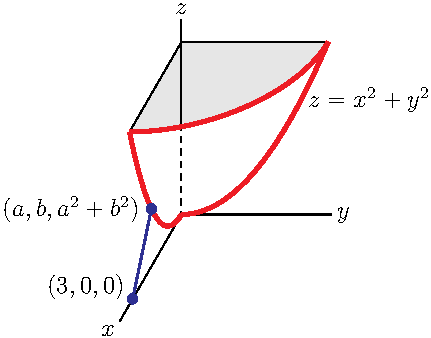
\includegraphics{distance.pdf}
\end{center}
}%
It crosses the plane at the value of $t$ which obeys
\begin{equation*}
\vn\cdot\vx(t)= c
\hskip .25 in\text{or}\hskip .25 in
\vn\cdot[\vp+t\vn]= c
\end{equation*}
namely
\begin{equation*}
t=[c-\vn\cdot\vp]/|\vn|^2
\end{equation*}
The vector
\begin{equation*}
\vx(t)-\vp=t\,\vn=\vn\,[c-\vn\cdot\vp]/|\vn|^2
\end{equation*}
has head on the plane $\vn\cdot\vx= c$, tail at $\vp$, and
is perpendicular to the plane. So the distance is the length of that
vector, which is
\begin{equation*}
|c-\vn\cdot\vp|/|\vn|
\end{equation*}
\end{solution}

%%%%%%%%%%%%%%%%%%%%%%%%%%%%%%%%%%%%
\begin{question}
Describe the set of points equidistant from $(1,2,3)$ and
$(5,2,7)$.
\end{question}

%\begin{hint}
%\end{hint}

\begin{answer}
It is the plane $x+z=8$, which is 
the plane through $(3,2,5)=\half(1,2,3)+\half(5,2,7)$ with normal 
$\llt 1,0,1\rgt=\frac{1}{4}\big(\llt 5,2,7\rgt-\llt 1,2,3\rgt \big)$.
\end{answer}

\begin{solution}
The distance from the point $(x,y,z)$ to $(1,2,3)$
is $\sqrt{(x-1)^2+(y-2)^2+(z-3)^2}$ and 
the distance from $(x,y,z)$to $(5,2,7)$ is
$\sqrt{(x-5)^2+(y-2)^2+(z-7)^2}$. Hence $(x,y,z)$ is equidistant 
from $(1,2,3)$ and $(5,2,7)$ if and only if
\begin{align*}
& & (x-1)^2+(y-2)^2+(z-3)^2&=(x-5)^2+(y-2)^2+(z-7)^2\\
&\iff & x^2-2x+1+z^2-6z+9&=x^2-10x+25+z^2-14z+49\\
&\iff & 8x+8z&=64\\
&\iff & x+z&=8
\end{align*}
This is the plane through $(3,2,5)=\half(1,2,3)+\half(5,2,7)$
with normal vector
$\llt 1,0,1\rgt=\frac{1}{4}\big(\llt 5,2,7\rgt-\llt 1,2,3\rgt \big)$.
\end{solution}

%%%%%%%%%%%%%%%%%%%%%%%%%%%%%%%%%%%%
\begin{question}
 Describe the set of points equidistant from $\va$ and $\vb$.
\end{question}

%\begin{hint}
%\end{hint}

\begin{answer}
It is the plane $2(\vb-\va)\cdot\vx=|\vb|^2-|\va|^2$,
which is the plane through $\half\va+\half\vb$
with normal vector  $\vb-\va$.
\end{answer}

\begin{solution}
The distance from the point $\vx$ to $\va$ is 
$\sqrt{(\vx-\va)\cdot(\vx-\va)}$ and the distance from $\vx$ to $\vb$ is
$\sqrt{(\vx-\vb)\cdot(\vx-\vb)}$. Hence $\vx$ is equidistant 
from $\va$ and $\vb$ if and only if
\begin{alignat*}{3}
& & (\vx-\va)\cdot(\vx-\va)&=(\vx-\vb)\cdot(\vx-\vb) \\
&\iff\qquad & |\vx|^2-2\va\cdot\vx+|\va|^2&=|\vx|^2-2\vb\cdot\vx+|\vb|^2 \\
&\iff & 2(\vb-\va)\cdot\vx&=|\vb|^2-|\va|^2
\end{alignat*}
This is the plane through $\half\va+\half\vb$
with normal vector  $\vb-\va$.
\end{solution}

%%%%%%%%%%%%%%%%%%%%%%%%%%%%%%%%%%%%
\begin{question} [M200 2003D] %1
Consider a point $P(5,-10,2)$ and the triangle with vertices
$A(0,1,1)$, $B(1,0,1)$ and $C(1,3,0)$.
\begin{enumerate}[(a)]
\item 
Compute the area of the triangle $ABC$.
\item
Find the distance from the point $P$ to the plane containing
the triangle. 
\end{enumerate}
\end{question}

%\begin{hint}
%\end{hint}

\begin{answer}
(a) $\half\sqrt{11}\approx 1.658$\qquad
(b) $\frac{3}{\sqrt{11}}\approx 0.9045$
\end{answer}

\begin{solution}
(a) One side of the triangle is 
      $\overrightarrow{AB}=\llt 1,0,1\rgt - \llt 0,1,1\rgt = \llt 1,-1,0\rgt$.
A second side of the triangle is 
      $\overrightarrow{AC}=\llt 1,3,0\rgt - \llt 0,1,1\rgt = \llt 1,2,-1\rgt$.
If the angle between $\overrightarrow{AB}$ and $\overrightarrow{AC}$
is $\theta$ and if we take $\overrightarrow{AB}$ as the base of the triangle,
then the triangle has base length $b=|\overrightarrow{AB}|$
and height $h=|\overrightarrow{AC}|\sin\theta$ and hence
\begin{equation*}
\text{area}=\half bh
=\half |\overrightarrow{AB}|\,|\overrightarrow{AC}|\sin\theta
=\half|\overrightarrow{AB}\times\overrightarrow{AC}|
=\half|\llt 1,-1,0\rgt \times \llt 1,2,-1\rgt|
\end{equation*}
As
\begin{equation*}
\llt 1,-1,0\rgt\times\llt 1,2,-1\rgt
=\det\left[\begin{matrix}
           \hi & \hj & \hk \\
            1  &  -1  &  0 \\
            1  &  2   &  -1
  \end{matrix}\right]
=\hi+\hj+3\hk
\end{equation*}
we have 
\begin{equation*}
\text{area}=\half|\llt 1,1,3\rgt|=\half\sqrt{11}\approx 1.658
\end{equation*}

(b) A unit vector perpendicular to the plane containing the 
triangle is
\begin{equation*}
\hn=\frac{\overrightarrow{AB}\times\overrightarrow{AC}}
            {|\overrightarrow{AB}\times\overrightarrow{AC}|}
=\frac{\llt 1,1,3\rgt}{\sqrt{11}}
\end{equation*}
The distance from $P$ to the plane containing the triangle is
the length of the projection of 
$\overrightarrow{AP}=\llt 5,-10,2\rgt-\llt 0,1,1\rgt
               =\llt 5,-11,1\rgt$ 
on $\hn$. If $\theta$ the angle between $\overrightarrow{AP}$
and $\hn$, then this is
\begin{equation*}
\text{distance}= |\overrightarrow{AP}|\,|\cos\theta| 
=\big|\overrightarrow{AP}\cdot\hn\big|
=\left|\llt 5,-11,1\rgt\cdot\frac{\llt 1,1,3\rgt}{\sqrt{11}}\right|
=\frac{3}{\sqrt{11}}\approx 0.9045
\end{equation*}
\end{solution}


%%%%%%%%%%%%%%%%%%%%%%%%%%%%%%%%%%%%%%%%%
\begin{question} [M200 2003A] % Bonus
Consider the sphere given by
$$
(x-1)^2+(y-2)^2+(z+1)^2=2
$$
Suppose that you are at the point $(2,2,0)$ on $S$, and you plan to follow
the shortest path on $S$ to $(2,1,-1)$. Express your initial direction
as a cross product.
\end{question}

%\begin{hint}
%
%\end{hint}

\begin{answer}
Any positive constant times
$\llt 1,1,-1\rgt\times\llt 1,0,1\rgt
=\llt 1, -2, -1\rgt$
\end{answer}

\begin{solution}
Switch to a new coordinate system with
$$
X=x-1\qquad Y=y-2\qquad Z=z+1
$$
In this new coordinate system, the sphere has equation $X^2+Y^2+Z^2=2$.
So the sphere is centred at $(X,Y,Z)=(0,0,0)$ and has radius $\sqrt{2}$.
In the new coordinate system, the initial point $(x,y,z)=(2,2,0)$
has $(X,Y,Z)=(1,0,1)$ and our final point  $(x,y,z)=(2,1,-1)$
has $(X,Y,Z)=(1,-1,0)$. Call the initial point $P$ and the final point
$Q$. The shortest path will follow the great circle from $P$ to $Q$.
\vadjust{
\begin{center}
     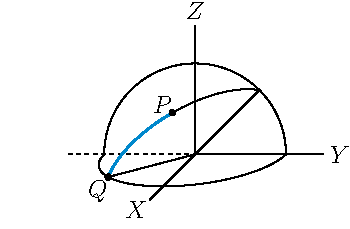
\includegraphics{OE03AQB.pdf}
\end{center}
}%
A great circle on a sphere is the intersection of the sphere with a plane
that contains the centre of the sphere. Our strategy for finding the initial
direction will be based on two observations.
\begin{itemize}
\item The shortest path lies on the plane $\Pi$ that contains the origin and the points $P$ and $Q$. Since the shortest path lies on $\Pi$,
our direction vector must also lie on $\Pi$ and hence must
be perpendicular to the normal vector to $\Pi$.
\item
The shortest path also remains on the sphere, so our initial direction
must also be perpendicular to the normal vector to 
the sphere at our initial point $P$. 
\end{itemize}
As our initial direction is perpendicular to the two normal vectors,
it is parallel to their cross product.

So our main job is to find normal vectors to the plane $\Pi$ and to the
sphere at $P$. 
\begin{itemize} 
\item One way to find a normal vector to $\Pi$ is to guess an equation for
$\Pi$. As $(0,0,0)$ is on $\Pi$, $(0,0,0)$ must obey $\Pi$'s equation.
So $\Pi$'s equation must be of the form $aX+bY+cZ=0$. That $(X,Y,Z)=(1,0,1)$ 
is on $\Pi$ forces $a+c=0$.   That $(X,Y,Z)=(1,-1,0)$ is on $\Pi$ forces 
$a-b=0$. So we may take $a=1$, $b=1$ and $c=-1$. That is, $\Pi$ is   
$X+Y-Z=0$.  (Check that all three points $(0,0,0)$, $(1,0,1)$ and
$(1,-1,0)$ do indeed obey $X+Y-Z=0$.) A normal vector to $\Pi$ is
$\llt 1,1,-1\rgt$.
\item A second way to find a normal vector to $\Pi$ is to observe that
both
\begin{itemize}
\item
the vector from $(0,0,0)$ to $(1,0,1)$, that is $\llt 1,0,1\rgt$, 
lies completely inside $\Pi$ and
\item
the vector from $(0,0,0)$ to $(1,-1,0)$, that is $\llt 1,-1,0\rgt$, 
lies completely inside $\Pi$.
\end{itemize}
So the vector
\begin{equation*}
\llt 1,0,1\rgt\times\llt 1,-1,0\rgt
=\det\left[\begin{matrix}
                     \hi & \hj & \hk \\
                     1   &  0  & 1 \\
                     1   &  -1  & 0
                \end{matrix}\right]
=\hi + \hj -\hk
\end{equation*}
is perpendicular to $\Pi$.
\item
The vector from the centre of the sphere to the point $P$ on the sphere
is perpendicular to the sphere at $P$. So a normal vector to 
the sphere at our initial point $(X,Y,Z)=(1,0,1)$ is $\llt 1,0,1\rgt$.
\end{itemize}
Since our initial direction\footnote{Note that the change of coordinates
$X=x-1$, $Y=y-2$, $Z=z+1$ has absolutely no effect on any velocity or direction
vector. If our position at time $t$ is $(x(t),y(t),z(t))$ in the
original coordinate system, then it is $(X(t),Y(t),Z(t))
=(x(t)-1,y(t)-2,z(t)+1)$ in the new coordinate system. The velocity
vectors in the two coordinate systems $\llt x'(t),y'(t),z'(t)\rgt
=\llt X'(t),Y'(t),Z'(t)\rgt$ are identical.}
must be perpendicular to both $\llt 1,1,-1\rgt$ and $\llt 1,0,1\rgt$, 
it must be one of  $\pm\llt 1,1,-1\rgt\times\llt 1,0,1\rgt$. 
To get from $(1,0,1)$ to $(1,-1,0)$ by the shortest path, our $Z$ 
coordinate should decrease from $1$ to $0$. So the $Z$ coordinate of 
our initial direction should be negative. This is the case for 
\begin{equation*}
\llt 1,1,-1\rgt\times\llt 1,0,1\rgt
=\det\left[\begin{matrix}
                     \hi & \hj & \hk \\
                     1   &  1  & -1 \\
                     1   &  0  &  1
                \end{matrix}\right]
=\hi - 2\,\hj -\hk
\end{equation*}
\end{solution}


\section{Equations of Lines in 3d}
%\documentclass[12pt]{article}

\questionheader{ex:s1.5}


%%%%%%%%%%%%%%%%%%
\subsection*{\Conceptual}
%%%%%%%%%%%%%%%%%%
%%%%%%%%%%%%%%%%%%%
\begin{question}
What is wrong with the following exercise?

``Give an equation for the line passing through the point $(3,1,3)$ that is normal to the vectors $\llt 4,-6,2 \rgt$ and $\llt \frac13,-\frac12,\frac16 \rgt$."
\end{question}
\begin{hint}
What's fishy about those normal vectors? 
\end{hint}
\begin{answer}
There are infinitely many planes satisfying the condition described, but we're asked for ``the" line.

We need two normal directions to figure out the direction of a line in $\mathbb R^3$. Since the given normal vectors are parallel to each other, they really only specify \emph{one} normal direction. 
\end{answer}
\begin{solution}
Note $12\llt \frac13,-\frac12,\frac16 \rgt=\llt 4,-6,2 \rgt$. So, we actually only know one normal direction to the line we're supposed to be describing. That means there are actually \emph{infinitely many} lines satisfying the given conditions.

\begin{center}
\begin{tikzpicture}
\draw[thick,->] (0,0) node[vertex]{}--(0,2.5) node[above]{$\mathbf n$};
\clip (3,0) arc (0:360:3cm and 1cm);
\draw (-3,0)--(3,0);
\draw (-3,-1)--(3,1);
\draw (-3,1)--(3,-1);
\draw (-3,-2)--(3,2) (-3,2)--(3,-2) (3,-3)--(-3,-3) (1,2)--(-1,-2) (1,-2)--(-1,2);
\end{tikzpicture}
\end{center}

\end{solution}
%%%%%%%%%%%%%%%%%%%

%%%%%%%%%%%%%%%%%%%
\begin{question}
Find, if possible, four lines in 3d with
\begin{itemize}
\item
   no two of the lines parallel to each other and
\item
   no two of the lines intersecting.
\end{itemize}
\end{question}

\begin{hint}
The two lines $\llt x-x_0\,,\,y-y_0\,,\,z-z_0\rgt =t\vd$ and
$\llt x-x'_0\,,\,y-y'_0\,,\,z-z'_0\rgt =t\vd'$ are not parallel if
$\vd\times\vd'\ne\vZero$.
\end{hint}


\begin{answer}
There are infinitely many correct answers. One is
\begin{align*}
\llt x\,,\,x\,,\,z-1\rgt &= t\llt 1,0,0\rgt &
\llt x\,,\,x\,,\,z-2\rgt &= t\llt 0,1,0\rgt \\
\llt x\,,\,x\,,\,z-3\rgt &= t\llt 1,1,0\rgt &
\llt x\,,\,x\,,\,z-4\rgt &= t\llt 1,-1,0\rgt 
\end{align*}
 
\end{answer}
\begin{solution}
There are infinitely many correct answers. One is
\begin{align*}
L_1:\ \llt x\,,\,x\,,\,z-1\rgt &= t\llt 1,0,0\rgt &
L_2:\ \llt x\,,\,x\,,\,z-2\rgt &= t\llt 0,1,0\rgt \\
L_3:\ \llt x\,,\,x\,,\,z-3\rgt &= t\llt 1,1,0\rgt &
L_4:\ \llt x\,,\,x\,,\,z-4\rgt &= t\llt 1,-1,0\rgt 
\end{align*}
No two of the lines are parallel because
\begin{itemize}
\item
$L_1$ and $L_2$ are not parallel because
$\llt 1,0,0\rgt\times \llt 0,1,0\rgt=\llt 0,0,1\rgt\ne\vZero$.
\item
$L_1$ and $L_3$ are not parallel because
$\llt 1,0,0\rgt\times \llt 1,1,0\rgt=\llt 0,0,1\rgt\ne\vZero$.
\item
$L_1$ and $L_4$ are not parallel because
$\llt 1,0,0\rgt\times \llt 1,-1,0\rgt=\llt 0,0,-1\rgt\ne\vZero$.
\item
$L_2$ and $L_3$ are not parallel because
$\llt 0,1,0\rgt\times \llt 1,1,0\rgt=\llt 0,0,-1\rgt\ne\vZero$.
\item
$L_2$ and $L_4$ are not parallel because
$\llt 0,1,0\rgt\times \llt 1,-1,0\rgt=\llt 0,0,-1\rgt\ne\vZero$.
\item
$L_3$ and $L_4$ are not parallel because
$\llt 1,1,0\rgt\times \llt 1,-1,0\rgt=\llt 0,0,-2\rgt\ne\vZero$.
\end{itemize}
No two of the lines intersect because
\begin{itemize}
\item every point on $L_1$ has $z=1$ and
\item every point on $L_2$ has $z=2$ and
\item every point on $L_3$ has $z=3$ and
\item every point on $L_4$ has $z=4$.
\end{itemize}
\end{solution}


%%%%%%%%%%%%%%%%%%%%%%%%%%%%
%\Instructions{Questions~\ref{prob_s1.0first} through \ref{prob_s1.0last} provide practice with.}
%%%%%%%%%%%%%%%%%%%%

%%%%%%%%%%%%%%%%%%
\subsection*{\Procedural}
%%%%%%%%%%%%%%%%%%

%%%%%%%%%%%%%%%%%%%%%%%%%%%%%%%%%%%%
\begin{question}
Find a vector parametric equation for the line of intersection
of the given planes.
\begin{enumerate}[(a)]
\item $x-2z=3$ and $y+\half z=5$
\item $2x-y-2z=-3$ and $4x-3y-3 z=-5$
\end{enumerate}
\end{question}

\begin{hint}
Review Example \eref{CLP200}{eg line equations} in the CLP-3 text.
\end{hint}

\begin{answer}
(a) $\llt x,y,z\rgt =  \llt 3,5,0\rgt+\llt 2,-\half,1\rgt t$

(b) $\llt x,y,z\rgt =  \llt -2,-1,0\rgt +\llt \frac{3}{2},1,1\rgt t$
\end{answer}

\begin{solution}
(a) The point $(x,y,z)$ obeys both $x-2z=3$ and $y+\half z=5$
if and only if $\llt x,y,z\rgt = \llt 3+2z, 5-\half z, z\rgt 
                  = \llt 3,5,0\rgt+\llt 2,-\half,1\rgt z$.
So, introducing a new variable $t$ obeying $t=z$, we get the vector 
parametric equation $\llt x,y,z\rgt =  \llt 3,5,0\rgt+\llt 2,-\half,1\rgt t$.

(b) The point $(x,y,z)$ obeys 
\begin{align*}
\left\{\Atop{2x-y-2z=-3}{4x-3y-3 z=-5} \right\}
&\iff \left\{\Atop{2x-y=2z-3}{4x-3y=3 z-5} \right\}
\iff\left\{\Atop{4x-2y=4z-6}{4x-3y=3 z-5} \right\}\\
\noalign{\vskip0.1in}
&\iff\left\{\Atop{4x-2y=4z-6}{y=z-1} \right\}
\end{align*}
Hence the point $(x,y,z)$ is on the line if and only if 
$\llt x,y,z\rgt = \llt \frac{1}{4}(2y+4z-6), z-1, z\rgt=
\llt \frac{3}{2}z-2, z-1, z\rgt = \llt -2,-1,0\rgt+\llt \frac{3}{2},1,1\rgt z$.
So, introducing a new variable $t$ obeying $t=z$, we get the vector 
parametric equation $\llt x,y,z\rgt =  \llt -2,-1,0\rgt
        +\llt \frac{3}{2},1,1\rgt t$.
\end{solution}

%%%%%%%%%%%%%%%%%%%%%%%%%%%%%%%%%%%%
\begin{question}
Determine a vector equation for the line of intersection
of the planes
\begin{enumerate}[(a)]
\item $x+y+z=3$ and $x+2y+3z=7$
\item $x+y+z=3$ and $2x+2y+2z=7$
\end{enumerate}
\end{question}

\begin{hint}
Review Example \eref{CLP200}{eg line equations} in the CLP-3 text.
\end{hint}

\begin{answer}
(a) $\llt x,y,z\rgt=\llt -1,4,0\rgt+t\llt 1,-2,1\rgt $

(b) The two planes are parallel and \emph{do not intersect}.

\end{answer}

\begin{solution}
(a) The normals to the two planes are $\llt 1,1,1\rgt $ and $\llt 1,2,3\rgt $
respectively. The line of intersection must have direction perpendicular
to both of these normals. Its direction vector is 
\begin{equation*}
\llt 1,1,1\rgt \times\llt 1,2,3\rgt 
=\det\left[\begin{matrix} \hi &\hj &\hk \\ 1&1&1 \\ 1&2&3 \end{matrix}\right]
=\llt 1,-2,1\rgt 
\end{equation*}
Substituting $z=0$ into the equations of the two planes and solving
\begin{align*}
\left\{\Atop{x+y=3}{x+2y=7} \right\}
&\iff \left\{\Atop{x=3-y}{x+2y=7} \right\}
\iff\left\{\Atop{x=3-y}{3-y+2y=7} \right\}
\end{align*}
we see that $z=0,\ y=4, x=-1$ lies on both planes. The line of
intersection is $\llt x,y,z\rgt=\llt -1,4,0\rgt+t\llt 1,-2,1\rgt $. 
This can be checked by verifying that,  for all values of $t$, 
$\llt x,y,z\rgt=\llt -1,4,0\rgt+t\llt 1,-2,1\rgt $ satisfies both 
$x+y+z=3$ and $x+2y+3z=7$.

(b) The equation $x+y+z=3$ is equivalent to $2x+2y+2z=6$.
So the two equations $x+y+z=3$ and $2x+2y+2z=7$ are mutually
contradictory. They have no solution. The two planes are parallel and
\emph{do not intersect}.
\end{solution}

%%%%%%%%%%%%%%%%%%%%%%%%%%%%%%%%%%%%
\begin{question}
In each case, determine whether or not the given pair
of lines intersect. Also find all planes containing the pair of lines.
\begin{enumerate}[(a)]
\item $\llt x,y,z\rgt = \llt -3,2,4\rgt+t\llt -4,2,1\rgt$ and 
      $\llt x,y,z\rgt = \llt 2,1,2\rgt+t\llt 1,1,-1\rgt$
\item $\llt x,y,z\rgt = \llt -3,2,4\rgt+t\llt -4,2,1\rgt$ and 
      $\llt x,y,z\rgt = \llt 2,1,-1\rgt+t\llt 1,1,-1\rgt$
\item $\llt x,y,z\rgt = \llt -3,2,4\rgt+t\llt -2,-2,2\rgt$ and 
      $\llt x,y,z\rgt = \llt 2,1,-1\rgt+t\llt 1,1,-1\rgt$
\item $\llt x,y,z\rgt = \llt 3,2,-2\rgt+t\llt -2,-2,2\rgt$ and 
      $\llt x,y,z\rgt = \llt 2,1,-1\rgt+t\llt 1,1,-1\rgt$
\end{enumerate}
\end{question}

%\begin{hint}
%\end{hint}

\begin{answer}
(a) $(1,0,3)$ lies on both lines.
     $x+y+2z=7$ is the only plane containing both lines.

(b) The two lines do not intersect. No plane contains the two lines.

(c) The two lines do not intersect.
     $x+z=1$ is the only plane containing both lines.

(d) The two lines are identical.
    For arbitrary $a$ and $b$ (not both zero) the plane $ax+by+(a+b)z=a$
    contains both lines.
\end{answer}

\begin{solution}
(a) Note that the value of the parameter $t$ in the 
equation $\llt x,y,z\rgt = \llt -3,2,4\rgt+t\llt -4,2,1\rgt$ 
need not have the same value as the parameter $t$ in the 
equation $\llt x,y,z\rgt = \llt 2,1,2\rgt+t\llt 1,1,-1\rgt$. So it is 
much safer to change the name of the parameter in the first equation 
from $t$ to $s$. In order for a point $(x,y,z)$ to lie on both 
lines we need
\begin{equation*}
\llt -3,2,4\rgt+s\llt -4,2,1\rgt = \llt 2,1,2\rgt+t\llt 1,1,-1\rgt
\end{equation*}
or equivalently, writing out the three component equations and moving
all $s$'s and $t$'s to the left and constants to the right,
\begin{align*}
-4s -t &= 5\\
2s -t &= -1\\
s +t &= -2
\end{align*}
Adding the last two equations together gives $3s=-3$ or $s=-1$. Substituting
this into the last equation gives $t=-1$. Note that $s=t=-1$ does indeed
satisfy all three equations so that 
 $\llt x,y,z\rgt=\llt -3,2,4\rgt-\llt -4,2,1\rgt=\llt 1,0,3\rgt$
lies on both lines. Any plane that contains the two lines must be parallel
to both direction vectors $\llt -4,2,1\rgt$ and $\llt 1,1,-1\rgt$. So 
its normal vector must be perpendicular to them, i.e. must be parallel to 
$\llt -4,2,1\rgt\times\llt 1,1,-1\rgt=\llt -3,-3,-6\rgt=-3\llt 1,1,2\rgt$. 
The plane must contain $(1,0,3)$ and be perpendicular to $\llt 1,1,2\rgt$. 
Its equation is $\llt 1,1,2\rgt\cdot\llt x-1,y,z-3\rgt=0$ or $x+y+2z=7$. 
This can be checked by verifying that $\llt -3,2,4\rgt+s\llt -4,2,1\rgt$ and 
$\llt 2,1,2\rgt+t\llt 1,1,-1\rgt$ obey
$x+y+2z=7$ for all $s$ and $t$ respectively. 

(b) In order for a point $(x,y,z)$ to lie on both lines we need
\begin{equation*}
\llt -3,2,4\rgt+s\llt -4,2,1\rgt = \llt 2,1,-1\rgt+t\llt 1,1,-1\rgt
\end{equation*}
or equivalently, writing out the three component equations and moving
all $s$'s and $t$'s to the left and constants to the right,
\begin{align*}
-4s -t &= 5\\
2s -t &= -1\\
s +t &= -5
\end{align*}
Adding the last two equations together gives $3s=-6$ or $s=-2$. Substituting
this into the last equation gives $t=-3$. However, substituting 
$s=-2,\ t=-3$ into the first equation gives $11=5$, which is impossible. The
two lines \emph{do not intersect}. In order for two lines to lie
in a common plane and not intersect, they must be parallel. So, in this
case \emph{no plane contains the two lines}.

(c) In order for a point $(x,y,z)$ to lie on both lines we need
\begin{equation*}
\llt -3,2,4\rgt+s\llt -2,-2,2\rgt = \llt 2,1,-1\rgt+t\llt 1,1,-1\rgt
\end{equation*}
or equivalently, writing out the three component equations and moving
all $s$'s and $t$'s to the left and constants to the right,
\begin{align*}
-2s -t &= 5\\
-2s -t &= -1\\
2s +t &= -5
\end{align*}
The first two equations are obviously contradictory. The
two lines \emph{do not intersect}. Any plane containing the two lines 
must be parallel to $\llt 1,1,-1\rgt$ (and hence automatically parallel
to $\llt -2,-2,2\rgt=-2\llt 1,1,-1\rgt$) and must also be parallel to the vector
from the point $(-3,2,4)$, which lies on the first line, to the point
$(2,1,-1)$, which lies on the second. The vector is $\llt 5,-1,-5\rgt$. 
Hence the normal to the plane is 
$\llt 5,-1,-5\rgt\times\llt 1,1,-1\rgt=\llt 6,0,6\rgt=6\llt 1,0,1\rgt$.
The plane perpendicular to $\llt 1,0,1\rgt$ containing $(2,1,-1)$ is
$\llt 1,0,1\rgt\cdot\llt x-2,y-1,z+1\rgt=0$ or $x+z=1$.

(d) Again the two lines are parallel, since 
$\llt -2,-2,2\rgt=-2\llt 1,1,-1\rgt$.
Furthermore the point 
$\llt 3,2,-2\rgt=\llt 3,2,-2\rgt+0\llt -2,-2,2\rgt
       =\llt 2,1,-1\rgt+1\llt 1,1,-1\rgt$
lies on both lines. So the two lines not only \emph{intersect} but
are identical. Any plane that contains the point $(3,2,-2)$ and is parallel
to $\llt 1,1,-1\rgt$ contains both lines. In general, the plane $ax+by+cz=d$
contains $(3,2,-2)$ if and only if $d=3a+2b-2c$ and is parallel to 
$\llt 1,1,-1\rgt$ if and only if $\llt a,b,c\rgt\cdot\llt 1,1,-1\rgt=a+b-c=0$. So, for arbitrary $a$ and $b$ (not both zero) $ax+by+(a+b)z=a$ works.
\end{solution}




%%%%%%%%%%%%%%%%%%%%%%%%%%%%%%%%
\begin{question}
Find the equation of the line through $(2,-1,-1)$ and parallel
to each of the two planes $x+y=0$ and $x-y+2z=0$. Express the equations
of the line in vector and scalar parametric forms and in symmetric form.
\end{question}

%\begin{hint}
%
%\end{hint}

\begin{answer}
vector parametric equation:\ \ \ $\llt x-2,y+1,z+1\rgt= t\llt 1,-1,-1\rgt$

scalar parametric equation:\ \ \ $x=2+t$,  $y=-1-t$,  $z=-1-t$

symmetric equation:\ \ \ $x-2=-y-1=-z-1$
\end{answer}

\begin{solution}
First observe that
\begin{itemize}
\item
$\llt 1,1,0\rgt$ is perpendicular to $x+y=0$  and hence to the line, and
\item
$\llt 1,-1,2\rgt$ is perpendicular to $x-y+2z=0$  and hence to the line.
\end{itemize}
Consequently
\begin{align*}
\llt 1\,,\,1\,,\,0\rgt \times \llt 1\,,\,-1\,,\,2\rgt
    =\det\left[\begin{matrix}
            \hi  &  \hj  &  \hk \\
            1    &   1   &   0 \\
            1    &  -1   &   2 
            \end{matrix}\right]
=\llt 2 \,,\, -2 \,,\, -2 \rgt
\end{align*}
is perpendicular to both $\llt 1,1,0\rgt$ and $\llt 1,-1,2\rgt$.
So $\frac{1}{2}\llt 2 \,,\, -2 \,,\, -2 \rgt=\llt 1,-1,-1\rgt\>$
is also perpendicular to both $\llt 1,1,0\rgt$ and $\llt 1,-1,2\rgt$
and hence is parallel to the line. As the point $(2,-1,-1)$ is on the line,
the vector  equation of the line is
\begin{equation*}
\llt x-2,y+1,z+1\rgt= t\llt 1,-1,-1\rgt
\end{equation*}
The scalar parametric equations for the line are
\begin{align*}
x-2=t,\ 
y+1=-t,\ 
z+1=-t
\hskip .25 in\hbox{or}\hskip .25 in
x=2+t,\ 
y=-1-t,\ 
z=-1-t
\end{align*}
The symmetric equations for the line are
\begin{align*}
(t=)\frac{x-2}{1}=\frac{y+1}{-1}=\frac{z+1}{-1}
\hskip .25 in\hbox{or}\hskip .25 in
x-2=-y-1=-z-1
\end{align*}


\end{solution}

%%%%%%%%%%%%%%%%%%%%%%%%%%%%%%%%
\begin{question}[M200 2011A] %1a
Let  $L$ be the line given by the equations $x + y = 1$ and
$x + 2y + z = 3$.
Write a vector parametric equation for $L$.
\end{question}

\begin{hint}
Review Example \eref{CLP200}{eg line equations} in the CLP-3 text.
\end{hint}

\begin{answer}
$\llt x,y,z\rgt = \llt 1,0,2\rgt +t\llt-1,1,-1 \rgt$
\end{answer}

\begin{solution}
Let's parametrize $L$ using $y$, renamed to $t$, as the parameter.
Then $y=t$, so that 
\begin{equation*}
x+y=1
\implies x+t=1
\implies x=1-t
\end{equation*}
and
\begin{equation*}
x+2y+z=3
\implies
1-t + 2t +z =3
\implies z = 2-t
\end{equation*}
and
\begin{equation*}
\llt x,y,z\rgt = \llt 1,0,2\rgt +t\llt-1,1,-1 \rgt
\end{equation*}
is a vector parametric equation for $L$.
\end{solution}

%%%%%%%%%%%%%%%%%%%%%%%%%%%%%%%%
\begin{question}
\begin{enumerate}[(a)]
\item
Find a vector parametric equation for the line
$x+2y+3z=11,\ x-2y+z=-1$. 
\item
Find the distance from $(1,0,1)$ to the line
$x+2y+3z=11,\ x-2y+z=-1$. 
\end{enumerate}
\end{question}

\begin{hint}
Review Example \eref{CLP200}{eg:VPdistance-point-line} in the CLP-3 text.
\end{hint}

\begin{answer}
(a) $\llt x,y,z\rgt=\llt 5,3,0\rgt+t\llt 4,1,-2\rgt =\llt 5+4t,3+t,-2t\rgt$.
\qquad
(b) $\sqrt{5}$
\end{answer}

\begin{solution} (a)
The normal vectors to the two given planes are 
$\llt 1,2,3\rgt $ and $\llt 1,-2,1\rgt $ respectively. 
Since the line is to be contained in both planes, its direction vector 
must be perpendicular to both $\llt 1,2,3\rgt $ and $\llt 1,-2,1\rgt $, 
and hence must be parallel to 
\begin{equation*}
\llt 1,2,3\rgt \times\llt 1,-2,1\rgt 
=\det\left[\begin{matrix}
           \hi & \hj & \hk \\
           1  &  2  &  3 \\
           1  &  -2  & 1
  \end{matrix}\right]
=\llt 8, 2,-4\rgt
\end{equation*} 
or to $\llt 4,1,-2\rgt $. Setting $z=0$ in $x+2y+3z=11,\ x-2y+z=-1$ and
solving 
\begin{align*}
\left\{\Atop{x+2y=11}{x-2y=-1} \right\}
\iff \left\{\Atop{2y=11-x}{x-2y=-1} \right\}
\iff \left\{\Atop{2y=11-x}{x-(11-x)=-1} \right\}
\iff \left\{\Atop{2y=11-x}{2x=10} \right\}
\end{align*}
we see that $(5,3,0)$ is on the line. So
the vector parametric equation of the line is 
$\llt x,y,z\rgt=\llt 5,3,0\rgt+t\llt 4,1,-2\rgt =\llt 5+4t,3+t,-2t\rgt$.


\noindent (b) 
The vector from $(1,0,1)$ to the point $(5+4t,3+t,-2t)$ on the line
is $\llt 4+4t,3+t,-1-2t\rgt$. In order for $(5+4t,3+t,-2t)$ to be the point 
of the line closest to $(1,0,1)$, the vector $\llt 4+4t,3+t,-1-2t\rgt$ 
joining those two points must be perpendicular to the direction vector 
$\llt 4,1,-2\rgt $ of the line. (See Example \eref{CLP200}{eg:VPdistance-point-line}  in the CLP-3 text.)
This is the case when
\begin{equation*}
\llt 4,1,-2\rgt \cdot \llt 4+4t,3+t,-1-2t\rgt =0\quad\text{or}\quad
16+16t+3+t+2+4t=0\quad\text{or}\quad t=-1
\end{equation*}
The point on the line nearest $(1,0,1)$ is thus 
$(5+4t,3+t,-2t)\Big|_{t=-1}=(5-4,3-1,2)=(1,2,2)$. The distance
from the point to the line is the length of the vector from
$(1,0,1)$ to the point on the line nearest $(1,0,1)$. That vector is 
$\llt 1,2,2\rgt -\llt 1,0,1\rgt =\llt 0,2,1\rgt$. So the distance is 
$|\llt 0,2,1\rgt|=\sqrt{5}$.
\end{solution}

%%%%%%%%%%%%%%%%%%%%%%%%%%%%%%%%
\begin{question}
Let $L_1$ be the line passing through $(1,-2,-5)$ in the direction of 
$\vd_1=\llt 2,3,2\rgt$. 
Let $L_2$ be the line passing through $(-3,4,-1)$ in the direction 
$\vd_2=\llt 5,2,4\rgt$.
\begin{enumerate}[(a)]
\item
Find the equation of the plane $P$ that contains $L_1$
and is parallel to $L_2$.
\item
Find the distance from $L_2$ to $P$.
\end{enumerate}
\end{question}

\begin{hint}
Review Example \eref{CLP200}{eg:VPdistance-point-plane} in the CLP-3 text.
\end{hint}

\begin{answer}
(a) $8x+2y-11z=59$\qquad
(b) $\frac{64}{\sqrt{189}} \approx 4.655$
\end{answer}

\begin{solution}
(a) The plane $P$ must be parallel to both $\llt 2,3,2\rgt $ (since it 
contains $L_1$) and $\llt 5,2,4\rgt $ (since it is parallel to $L_2$).
Hence 
\begin{equation*}
\llt 2,3,2\rgt \times \llt 5,2,4\rgt 
=\det\left[\begin{matrix}
           \hi & \hj & \hk \\
           2  &  3  & 2 \\
           5  &  2  & 4
  \end{matrix}\right]
=\llt 8,2,-11\rgt 
\end{equation*}
is normal to $P$. As the point $(1,-2,-5)$ is on $P$, the equation
of $P$ is
\begin{equation*}
\llt 8,2,-11\rgt \cdot\llt x-1,y+2,z+5\rgt =0\qquad \text{or}\qquad 8x+2y-11z=59
\end{equation*}

(b) As $L_2$ is parallel to $P$, the distance from $L_2$ to $P$ is the
same as the distance from any one point of $L_2$, for example $(-3,4,-1)$,
to $P$. As $(1,-2,-5)$ is a point on $P$, the vector 
$\llt 1,-2,-5\rgt-\llt -3, 4,-1\rgt =\llt 4,-6,-4\rgt $ has its head on $P$ 
and tail at $(-3,4,-1)$ on $L_2$. 
The distance from $L_2$ to $P$ is the length of the projection of the vector $\llt 4,-6,-4\rgt $ on the normal to $P$. (See Example \eref{CLP200}{eg:VPdistance-point-plane-bis} in the CLP-3 text.) This is 
\begin{equation*}
\left|\text{proj}_{\llt 8,2,-11\rgt}\llt 4,-6,-4\rgt\right|
=\frac{|\llt 4,-6,-4\rgt \cdot\llt 8,2,-11\rgt|} {|\llt 8,2,-11\rgt|}
=\frac{64}{\sqrt{189}}
\approx4.655
\end{equation*}
\end{solution}


%%%%%%%%%%%%%%%%%%%%%%%%%%%%%%%%
\begin{question}[M200 2012a] %1
Let $L$ be a line which is parallel to the plane $2x + y  - z = 5$ and 
perpendicular to the line $x = 3 - t$, $y = 1 - 2t$ and $z = 3t$.
\begin{enumerate}[(a)]
\item
Find a vector parallel to the line $L$.
\item
Find parametric equations for the line $L$ if $L$ passes through a point 
$Q(a, b, c)$
where $a < 0$, $b > 0$, $c > 0$, and the distances from $Q$ to the $xy$--plane, 
the $xz$--plane and the $yz$--plane are $2$, $3$ and $4$ respectively.
\end{enumerate}
\end{question}

%\begin{hint}
%
%\end{hint}

\begin{answer}
(a) Any nonzero constant times $\llt 1 \,,\, -5 \,,\, -3 \rgt$.\qquad
(b) $x = -4 + t$, 
    $y = 3 - 5t$,
    $z = 2 - 3t$
\end{answer}

\begin{solution}
(a) The line $L$ must be perpendicular both to 
        $\llt 2\,,\,1\,,\,-1\rgt$, which is a normal vector 
        for the plane $2x + y  - z = 5$,
and to
        $\llt -1\,,\,-2\,,\,3\rgt$, which is a direction vector for
the line $x = 3 - t$, $y = 1 - 2t$ and $z = 3t$.
Any such vector must be a nonzero constant times
\begin{align*}
\llt 2\,,\,1\,,\,-1\rgt \times \llt -1\,,\,-2\,,\,3\rgt
    =\det\left[\begin{matrix}
            \hi  &  \hj  &  \hk \\
            2    &   1   &    -1 \\
           -1    &  -2   &   3 
            \end{matrix}\right]
=\llt 1 \,,\, -5 \,,\, -3 \rgt
\end{align*}

(b) For the point $Q(a, b, c)$
\begin{itemize}
\item
to be a distance $2$ from the $xy$--plane, it is necessary that $|c|=2$,
and
\item
to be a distance $3$ from the $xz$--plane, it is necessary that $|b|=3$,
and
\item
to be a distance $4$ from the $yz$--plane, it is necessary that $|a|=4$.
\end{itemize}
As $a < 0$, $b > 0$, $c > 0$, the point $Q$ is $(-4, 3, 2)$ and the line $L$
is
\begin{equation*}
x = -4 + t \qquad
y = 3 - 5t \qquad
z = 2 - 3t 
\end{equation*}
\end{solution}

%%%%%%%%%%%%%%%%%%%%%%%%%%%%%%%%
\begin{question}[M200 2012D] %1
Let $L$ be the line of intersection of the planes $x + y + z = 6$ and 
$x - y + 2z = 0$.
\begin{enumerate}[(a)]
\item
Find the points in which the line $L$ intersects the coordinate planes.
\item
Find parametric equations for the line through the point $(10, 11, 13)$ 
that is perpendicular to the line $L$ and parallel to the plane $y = z$.
\end{enumerate}
\end{question}

%\begin{hint}
%
%\end{hint}

\begin{answer}
(a) $(3,3,0)$,  $(12,0,-6)$, $(0,4,2)$ \qquad
(b) $x=10+t$, $y=11+t$, $z=13+t$.
\end{answer}

\begin{solution}
(a)
The line $L$ intersects the $xy$--plane when 
$x + y + z = 6$,
$x - y + 2z = 0$,
and $z=0$. When $z=0$ the equations of $L$ reduce to 
$x + y = 6$,
$x - y = 0$.
So the intersection point is $(3,3,0)$.

The line $L$ intersects the $xz$--plane when 
$x + y + z = 6$,
$x - y + 2z = 0$,
and $y=0$. When $y=0$ the equations of $L$ reduce to 
$x + z = 6$,
$x +2z = 0$.
Substituting $x=-2z$ into $x+z=6$ gives $-z=6$.
So the intersection point is $(12,0,-6)$.

The line $L$ intersects the $yz$--plane when 
$x + y + z = 6$,
$x - y + 2z = 0$,
and $x=0$. When $x=0$ the equations of $L$ reduce to 
$y + z = 6$,
$-y +2z = 0$.
Substituting $y=2z$ into $y+z=6$ gives $3z=6$.
So the intersection point is $(0,4,2)$.

(b)
Our main job is to find a direction vector $\vd$ for the line.
\begin{itemize}
\item
Since the line is to be parallel to $y=z$, $\vd$ must be perpendicular
to the normal vector for $y=z$, which is $\llt 0,1,-1\rgt$. 
\item
$\vd$ must also be perpendicular to $L$. For a point $(x,y,z)$ to be on $L$
it must obey $x+y = 6-z$ and $x-y =-2z$. Adding these two equations
gives $2x=6-3z$ and subtracting the second equation from the first
gives $2y= 6+z$. So for a point $(x,y,z)$ to be on $L$ it must obey 
$x=3-\frac{3z}{2}$, $y=3+\frac{z}{2}$. The point on $L$ with $z=0$
is $(3,3,0)$ and the point on $L$ with $z=2$ is $(0,4,2)$. So
 $\llt 0-3,4-3,2-0 \rgt=\llt -3,1,2 \rgt$ is a direction vector for $L$.
\end{itemize}
So $\vd$ must be perpendicular to both $\llt 0,1,-1\rgt$
and $\llt -3,1,2 \rgt$ and so must be a nonzero constant times
\begin{align*}
\llt 0,1,-1\rgt \times \llt -3,1,2 \rgt
    =\det\left[\begin{matrix}
            \hi  &  \hj  &  \hk \\
            0    &   1   &   -1 \\
            -3    &   1   &    2 
            \end{matrix}\right]
=\llt 3 \,,\, 3 \,,\, 3 \rgt
\end{align*}
We choose $\vd=\frac{1}{3}\llt 3 \,,\, 3 \,,\, 3 \rgt=\llt 1\,,\,1\,,\,1 \rgt$.
So 
\begin{equation*}
\llt x,y,z\rgt = \llt 10,11,13\rgt + t \llt 1\,,\,1\,,\,1 \rgt
\end{equation*}
is a vector parametric equation for the line. We can also write this as
$x=10+t$, $y=11+t$, $z=13+t$.
\end{solution}

%%%%%%%%%%%%%%%%%%%%%%%%%%%%%%%%
\begin{question}[M200 2013D] %1a
The line $L$ has vector parametric equation 
$\vr(t) = (2 + 3t)\hi + 4t\hj - \hk$.
\begin{enumerate}[(a)]
\item
Write the symmetric equations for $L$.
\item
Let $\alpha$ be the angle between the line $L$ and the plane given 
by the equation $x - y + 2z = 0$. Find $\alpha$.
\end{enumerate}
\end{question}

\begin{hint}
Review the properties of the dot product in 
Theorem \eref{CLP200}{thm:dotPppties} of the CLP-3 text.
\end{hint}

\begin{answer}
(a)  $\frac{x-2}{3}=\frac{y}{4}\qquad z=-1$

(b)  $\al =\frac{\pi}{2}-\arccos\frac{1}{5\sqrt{6}}
             \approx 0.08\,\text{radians}$
\end{answer}

\begin{solution}
(a)  Since
\begin{alignat*}{3}
x&=2+3t &&\implies t=\frac{x-2}{3} \\
y&=4t   &&\implies t=\frac{y}{4}
\end{alignat*}
we have
\begin{equation*}
\frac{x-2}{3}=\frac{y}{4}\qquad z=-1
\end{equation*}

(b) The direction vector for the line 
   $\vr(t) = 2\,\hi-\hk +t(3\,\hi+4\,\hj)$
  is $\vd=3\,\hi+4\,\hj$. A normal vector for the plane $x-y+2z=0$ is 
   $\vn=\pm\big(\hi-\hj+2\,\hk\big)$. The angle $\theta$ between $\vd$ 
   and $\vn$ obeys
\begin{align*}
\cos\theta =\frac{\vd\cdot\vn}{|\vd|\,|\vn|}
           =\frac{1}{5\sqrt{6}}
\implies \theta =\arccos\frac{1}{5\sqrt{6}}\approx 1.49\,\text{radians}
\end{align*}
(We picked $\vn=-\hi+\hj-2\hk$ to make $0\le\theta\le\frac{\pi}{2}$.)
Then the angle between $\vd$ and the plane is
\begin{equation*}
\al =\frac{\pi}{2}-\arccos\frac{1}{5\sqrt{6}}\approx 0.08\,\text{radians}
\end{equation*}

\begin{center}
     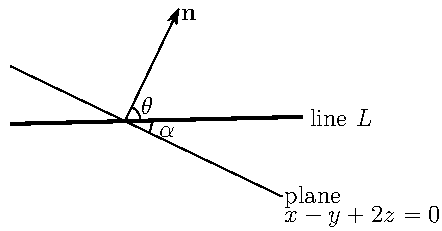
\includegraphics{fig/OE13D_1.pdf}
\end{center}


\end{solution}

%%%%%%%%%%%%%%%%%%%%%%%%%%%%%%%%
\begin{question}[M200 2015D] %1b
Find the parametric equation for the line of intersection of the 
planes
\begin{equation*}
x + y + z = 11\qquad \text{and}\qquad x - y - z = 13.
\end{equation*}
\end{question}

%\begin{hint}
%
%\end{hint}

\begin{answer}
$(x,y,z) = \big(12\,,\,-1-t\,,\,t\big)$
\end{answer}

\begin{solution}
Let's use $z$ as the parameter and call it $t$. Then $z=t$
and
\begin{align*}
x+y&=11-t \\
x-y&=13+t
\end{align*}
Adding the two equations gives $2x=24$ and subtracting the
second equation from the first gives $2y=-2-2t$. So
\begin{equation*}
(x,y,z) = \big(12\,,\,-1-t\,,\,t\big)
\end{equation*}
\end{solution}

%%%%%%%%%%%%%%%%%%%%%%%%%%%%%%%%
\begin{question}[M200 2000A] %1
\begin{enumerate}[(a)]
\item
Find a point on the y-axis equidistant from 
                $(2, 5, -3)$ and $(-3, 6, 1)$. 

\item  
Find the equation of the plane containing the point 
           $(1, 3, 1)$ and the line $\vr(t) = t\,\hi + t\,\hj + (t + 2)\,\hk$.
\end{enumerate}
\end{question}

%\begin{hint}
%
%\end{hint}

\begin{answer}
(a) $(0,4,0)$\qquad
(b) $2x-y-z=-2$
\end{answer}

\begin{solution}
(a) 
The point $(0,y,0)$, on the $y$--axis, is equidistant from 
                $(2, 5, -3)$ and $(-3, 6, 1)$ if and only if
\begin{align*}
&\big|\llt 2, 5, -3\rgt-\llt 0,y,0\rgt\big|
         =\big|\llt -3, 6, 1\rgt-\llt 0,y,0\rgt\big| \\
&\iff 2^2+(5-y)^2+(-3)^2=(-3)^2+(6-y)^2+1^2 \\
&\iff 2y=8 \\
&\iff y=4
\end{align*}

(b) 
The points $(1,3,1)$ and $\vr(0)=(0,0,2)$ are both on the plane.
Hence the vector $\llt 1,3,1\rgt-\llt 0,0,2\rgt=\llt 1,3,-1\rgt$ 
joining them,
and the direction vector of the line, namely $\llt 1,1,1\rgt$ are 
both parallel to the plane. So 
\begin{equation*}
\llt 1,3,-1\rgt\times \llt 1,1,1\rgt
=\det\left[\begin{matrix} \hi &\hj &\hk \\ 
                           1&3&-1 \\ 
                           1&1&1 \end{matrix}\right]
= \llt 4,-2,-2\rgt
\end{equation*}
is perpendicular to the plane. As the point $(0,0,2)$ is on the plane
and the vector  $\llt 4,-2,-2\rgt$ is perpendicular to the plane, the
equation of the plane is
\begin{equation*}
4(x-0)-2(y-0)-2(z-2)=0\text{ or } 2x-y-z=-2
\end{equation*}
\end{solution}


%%%%%%%%%%%%%%%%%%
\subsection*{\Application}
%%%%%%%%%%%%%%%%%%


%%%%%%%%%%%%%%%%%%%%%%%%%%%%%%%%
\begin{question}[M200 2016D] %1
Let $A=(0,2,2)$, $B=(2,2,2)$, $C=(5,2,1)$.
\begin{enumerate}[(a)]
\item
Find the parametric equations for the line which contains $A$
and is perpendicular to the triangle $ABC$.
\item
Find the equation of the set of all points $P$ such that $\overrightarrow{PA}$
is perpendicular to $\overrightarrow{PB}$. This set forms a
Plane/Line/Sphere/Cone/Paraboloid/Hyperboloid (circle one) in
space.
\item
A light source at the origin shines on the triangle $ABC$ making
a shadow on the plane $x+7y+z=32$. (See the diagram.) Find $\tilde A$.

\begin{center}
     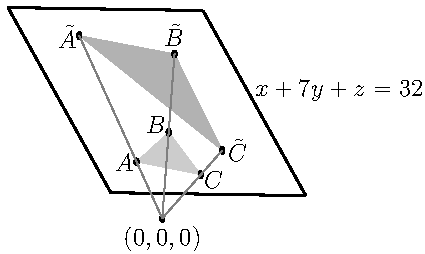
\includegraphics{fig/OE16D_1.pdf}
\end{center}


\end{enumerate}
\end{question}

\begin{hint}
All three of the points $A$, $B$, $C$ lie in the plane $y=2$.
\end{hint}

\begin{answer}
(a) $x=0,\ y=2+t,\ z=2$\qquad
(b) The sphere $(x-1)^2 +(y-2)^2+(z-2)^2 = 1$

(c) $(0,4,4)$
\end{answer}

\begin{solution}
(a) We are given one point on the line, so we just need a
direction vector. That direction vector has to be perpendicular to the 
triangle $ABC$.

The fast way to get a direction vector is to observe that all 
three points $A$, $B$ and $C$, and consequently the entire triangle $ABC$,
are contained in the plane $y=2$. A normal vector to that plane, and 
consequently a direction vector for the desired line, is $\hj$.

Here is another, more mechanical, way to get a direction vector.
The vector from $A$ to $B$ is $\llt 2-0\,,\,2-2\,,\,2-2\rgt= \llt 2,0,0\rgt$
and the vector from $A$ to $C$ is $\llt 5-0\,,\,2-2\,,\,1-2\rgt= 
\llt 5,0,-1\rgt$. So a vector perpendicular to the triangle $ABC$ is
\begin{align*}
\llt 2,0,0\rgt \times \llt 5,0,-1\rgt
=\det\left[\begin{matrix}
            \hi  &  \hj  &  \hk \\
            2    &   0   &    0 \\
            5    &   0   &   -1 
            \end{matrix}\right]
=\llt 0 \,,\, 2 \,,\, 0 \rgt
\end{align*}
The vector $\frac{1}{2}\llt 0 \,,\, 2 \,,\, 0 \rgt=\llt 0 \,,\, 1 \,,\, 0 \rgt$
is also perpendicular to the triangle $ABC$. 

So the specified line has to contain the point $(0,2,2)$ and have direction
vector $\llt 0 , 1 , 0 \rgt$. The parametric equations
\begin{align*}
\llt x,y,z \rgt = \llt 0 , 2 , 2 \rgt + t\llt 0 , 1 , 0 \rgt
\end{align*}
or
\begin{align*}
x=0,\ 
y=2+t,\ 
z=2
\end{align*}
do the job.


\goodbreak
(b) Let $P$ be the point $(x,y,z)$. Then the vector from  $P$ to $A$
is $\llt 0-x\,,\,2-y\,,\,2-z\rgt$ and the vector from  $P$ to $B$
is $\llt 2-x\,,\,2-y\,,\,2-z\rgt$. These two vector are perpendicular
if and only if
\begin{align*}
0 &= \llt -x\,,\,2-y\,,\,2-z\rgt \cdot \llt 2-x\,,\,2-y\,,\,2-z\rgt
  = x(x-2) +(y-2)^2 +(z-2)^2 \\
  &= (x-1)^2 -1 +(y-2)^2 +(z-2)^2 
\end{align*}
This is a sphere.

(c) 
The light ray that forms $\tilde A$ starts at the origin,
passes through $A$ and then intersects the plane $x+7y+z=32$
at $\tilde A$. The line from the origin through $A$ has vector
parametric equation
\begin{align*}
\llt x,y,z\rgt = \llt 0,0,0 \rgt +t \llt 0,2,2\rgt
               =\llt 0,2t,2t\rgt
\end{align*}
This line intersects the plane $x+7y+z=32$ at the point whose value of $t$
obeys
\begin{align*}
(0) +7\overbrace{(2t)}^{y} +\overbrace{(2t)}^{z} =32
\iff t=2
\end{align*}
So $\tilde A$ is $(0,4,4)$.
\end{solution}

%%%%%%%%%%%%%%%%%%%%%%%%%%%%%%%%
\begin{question}
Let $P,\ Q,\ R$ and $S$ be the vertices of a tetrahedron.
Denote by $\vp,\ \vq,\ \vr$ and $\vs$ the vectors from the origin
to $P,\ Q,\ R$ and $S$ respectively. A line is drawn from each vertex to
the centroid of the opposite face, where the centroid of a triangle with 
vertices $\va,\ \vb$ and $\vc$ is $\frac{1}{3}(\va+\vb+\vc)$. 
Show that these four lines meet at $\frac{1}{4}(\vp+\vq+\vr+\vs$).
\end{question}

%\begin{hint}
%
%\end{hint}

\begin{answer}
See the solution.
\end{answer}

\begin{solution}
The face opposite $\vp$ is the triangle with vertices $\vq$, $\vr$ and $\vs$. 
The centroid of this triangle is $\frac{1}{3}(\vq+\vr+\vs)$. 
The direction vector of the line through $\vp$ and the 
centroid $\frac{1}{3}(\vq+\vr+\vs)$ is 
$\frac{1}{3}(\vq+\vr+\vs)-\vp$. The points on the line through
$\vp$ and the centroid $\frac{1}{3}(\vq+\vr+\vs)$ are those
of the form
\begin{equation*}
\vx=\vp+ t\left[\frac{1}{3}(\vq+\vr+\vs)-\vp\right]
\end{equation*}
for some real number $t$. Observe that when $t=\frac{3}{4}$
$$
\vp+ t\left[\frac{1}{3}(\vq+\vr+\vs)-\vp\right]
=\frac{1}{4}(\vp+\vq+\vr+\vs)
$$
so that $\frac{1}{4}(\vp+\vq+\vr+\vs)$ is on the line.
The other three lines have vector parametric equations
\begin{align*}
\vx&=\vq+ t\left[\frac{1}{3}(\vp+\vr+\vs)-\vq\right] \\
\vx&=\vr+ t\left[\frac{1}{3}(\vp+\vq+\vs)-\vr\right] \\
\vx&=\vs+ t\left[\frac{1}{3}(\vp+\vq+\vr)-\vs\right]
\end{align*}
When $t=\frac{3}{4}$, each of the three right hand sides also reduces
to $\frac{1}{4}(\vp+\vq+\vr+\vs)$ so that
$\frac{1}{4}(\vp+\vq+\vr+\vs)$ is also on each of these
three lines.
\end{solution}


%%%%%%%%%%%%%%%%%%%%%%%%%%%%%%%%
\begin{question}
Calculate the distance between the lines 
$\frac{x+2}{3}=\frac{y-7}{-4}=\frac{z-2}{4}$ and $\frac{x-1}{-3}=\frac{y+2}{4}=\frac{z+1}{1}$.
\end{question}

\begin{hint}
Review Example \eref{CLP200}{eg:VPdistance-line-line-bis}
in the CLP-3 text.
\end{hint}

\begin{answer}
$3$
\end{answer}

\begin{solution}
We'll use the procedure of Example \eref{CLP200}{eg:VPdistance-line-line-bis}
in the CLP-3 text. 
The vector 
\begin{equation*}
\llt 3,-4,4\rgt \times\llt -3,4,1\rgt 
=\det\left[\begin{matrix}
           \hi & \hj & \hk \\
           3  &  -4  &  4 \\
          -3  &   4  & 1
  \end{matrix}\right]
=\llt -20,-15,0\rgt 
\end{equation*}
is perpendicular to both lines. Hence so is 
$\vn=-\frac{1}{5}\llt -20,-15,0\rgt =\llt 4,3,0\rgt $. The point
$(-2,7,2)$ is on the first line and the point $(1,-2,-1)$ is on the second
line. Hence 
$\vv=\llt -2,7,2 \rgt-\llt1,-2,-1 \rgt=\llt -3,9,3\rgt $ is a vector 
joining the two lines. 
The desired distance is the length of the projection of $\vv$ on $\vn$. 
This is 
\begin{equation*}
\big|{\rm proj}_{\vn}\vv\big|
=\frac{|\llt -3,9,3\rgt \cdot\llt 4,3,0\rgt|}{|\llt 4,3,0\rgt|} 
=\frac{15}{5}=3
\end{equation*}
\end{solution}



%\setcounter{section}{6}
\section{Curves and their Tangent Vectors}
%\documentclass[12pt]{article}

\questionheader{ex:s1.6}

%%%%%%%%%%%%%%%%%%%
%\subsection*{Derivatives, Velocity, Etc.}
%%%%%%%%%%%%%%%%%%%


%%%%%%%%%%%%%%%%%%
\subsection*{\Conceptual}
%%%%%%%%%%%%%%%%%%

%%%%%%%%%%%%%%%%%%%%%%%%%%%
\Instructions{Questions~\ref{prob_s1.0first} through \ref{prob_s1.0last} provide practice with curve parametrization. Being comfortable with the 
algebra and interpretation of these descriptions are essential ingredients 
in working effectively with parametrizations.}
%%%%%%%%%%%%%%%%%%%
\begin{question}\label{prob_s1.0first}
Consider the following time-parametrized curve:
\[\vr(t)=\left( \cos\left(\frac{\pi}{4}t\right)~,~(t-5)^2\right)\]

List the three points $(-1/\sqrt{2},0)$, $(1,25)$, and $(0,25)$ in chronological order.
\end{question}
\begin{hint}
Find the value of $t$ at which the three points occur on the curve.
\end{hint}
\begin{answer}
$(1,25)$, $(-1/\sqrt2,0)$, $(0,25)$.
\end{answer}
\begin{solution}
We can find the time at which the curve hits a given point by considering the two equations that arise from the two coordinates. For the $y$-coordinate to be 0, we must have $(t-5)^2=0$, i.e. $t=5$. So, the point $(-1/\sqrt{2},0)$ happens when $t=5$.

Similarly, for the $y$-coordinate to be $25$,  we need $(t-5)^2=25$, so $(t-5)=\pm 5$.
When $t=0$, the curve hits $(1, 25)$; when $t=10$, the curve hits $(0,25)$.

So, in order, the curve passes through the points $(1,25)$, $(-1/\sqrt2,0)$, and $(0,25)$.
\end{solution}
%%%%%%%%%%%%%%%%%%%

\begin{question}
At what points in the $xy$-plane does the curve $(\sin t, t^2)$ cross itself? What is the difference in $t$ between the first time the curve crosses through a point, and the last?
\end{question}
\begin{hint}
The curve ``crosses itself" when $(\sin t,t^2)$ gives the same coordinate for different values of $t$. When these crossings occur will depend on which crossing you're referring to, so your answers should all depend on $t$.
\end{hint}
\begin{answer}
The curve crosses itself at all points $(0,(\pi n)^2)$ where $n$ is an integer. It passes such a point twice, $2\pi n$ time units apart.
\end{answer}
\begin{solution}
The curve ``crosses itself" when the same coordinates occur for different values of $t$, say $t_1$ and $t_2$. So, we want to know when $\sin t_1=\sin t_2$ and also $t_1^2=t_2^2$. Since $t_1$ and $t_2$ should be different, the second equation tells us $t_2=-t_1$. Then the first equation tells us $\sin t_1=\sin t_2=\sin(-t_1)=-\sin t_1$. That is, $\sin t_1 = -\sin t_1$, so $\sin t_1=0$. That happens whenever $t_1=\pi n$ for an integer $n$.

So, the points at which the curve crosses itself are those points $(0,(\pi n)^2)$ where $n$ is an integer. It passes such a point at times $t=\pi n $ and $t=-\pi n$. So, the curve hits this point $2\pi n$ time units apart.
\end{solution}

%%%%%%%%%%%%%%%%%%%%%%%%%%%%%%%
\begin{question}
Find the specified parametrization of the first quadrant part
of the circle $x^2+y^2=a^2$.
\begin{enumerate}[(a)]
\item 
  In terms of the $y$ coordinate.
\item
  In terms of the angle between the tangent line and the 
  positive $x$-axis.
\item
  In terms of the arc length from $(0,a)$.
\end{enumerate}
\end{question}

\begin{hint} 
Draw sketches. Don't forget the range that the parameter runs over.
\end{hint}

\begin{answer} 
(a) $\vr(y)=\sqrt{a^2-y^2}\,\hi+ y\,\hj$, $0\le y\le a$

(b) $\big(x(\phi),y(\phi)\big)
       =\big(a\sin \phi ,-a\cos \phi \big)$,
   $\frac{\pi}{2}\le\phi\le\pi$

(c) $\big(x(s),y(s)\big)
    =\big(a\cos(\tfrac{\pi}{2}-\frac{s}{a}),
           a\sin(\tfrac{\pi}{2}-\tfrac{s}{a})\big)$,
   $0\le s\le\tfrac{\pi}{2}a$
\end{answer}

\begin{solution} 
(a) 
Since, on the specified part of the  circle, 
$x=\sqrt{a^2-y^2}$ and  $y$ runs from $0$ to $a$, 
the parametrization is
$\vr(y)=\sqrt{a^2-y^2}\,\hi+ y\,\hj$, $0\le y\le a$.

(b) Let $\theta$ be the angle between 
\begin{itemize}\itemsep1pt \parskip0pt \parsep0pt
\item the radius vector from the origin to the point 
$(a\cos\theta,a\sin\theta)$  on the circle and 
\item
the positive $x$-axis. 
\end{itemize}
The tangent line to the circle at $(a\cos\theta,a\sin\theta)$ 
is perpendicular to the radius vector and so makes angle $\phi=\frac{\pi}{2}+\theta$ with the positive $x$ axis.
(See the figure on the left below.)
As $\theta =\phi-\frac{\pi}{2}$, the desired parametrization is
\begin{equation*}
\big(x(\phi),y(\phi)\big)
=\big(a\cos(\phi-\tfrac{\pi}{2}),a\sin(\phi-\tfrac{\pi}{2})\big)
=\big(a\sin \phi ,-a\cos \phi \big),\ 
  \tfrac{\pi}{2}\le\phi\le\pi
\end{equation*}

\begin{center}
       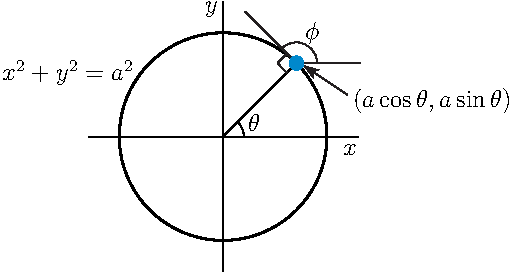
\includegraphics{parCirclePhi.pdf}\quad
       \includegraphics{parCircleS.pdf}
\end{center}


(c) Let $\theta$ be the angle between 
\begin{itemize}\itemsep1pt \parskip0pt \parsep0pt
\item the radius vector from the origin to the point 
$(a\cos\theta,a\sin\theta)$  on the circle and 
\item
the positive $x$-axis. 
\end{itemize} 
The arc from $(0,a)$ to $(a\cos\theta,a\sin\theta)$ 
subtends an angle $\frac{\pi}{2}-\theta$ and so
has length $s=a\big(\frac{\pi}{2}-\theta\big)$. (See the figure
on the right above.) Thus $\theta=\frac{\pi}{2}-\frac{s}{a}$
and the desired parametrization is
\begin{equation*}
\big(x(s),y(s)\big)
=\left(a\cos\left(\frac{\pi}{2}-\frac{s}{a}\right)\,,\,
           a\sin\left(\frac{\pi}{2}-\frac{s}{a}\right)\right)
,\ 0\le s\le\frac{\pi}{2}a
\end{equation*}
\end{solution}


%%%%%%%%%%%%%%%%%%%%%%%%%%%%%%%%%%%%%%
\begin{question}\label{prob_s1.1_cycloid}

\begin{center}
\begin{tikzpicture}
\YEaaxis{1}{13}{.5}{3}
\YExcoord{1}{1}
\YEycoord{1}{1}
\draw[thick] (1,2) node[red,vertex, label=above:{\textcolor{red}{$P$}}]{} arc (90:450:1cm);
\foreach \x in {0,1,2,3,4}{
	\MULTIPLY{\x}{.2}{\y}
	\SUBTRACT{1}{\y}{\o}
	\MULTIPLY{\x}{2.25}{\z}
	\MULTIPLY{\z}{57.3}{\zrad}
	\draw[red,opacity=\o] ({1+\z+sin(\zrad)},{1+cos(\zrad)}) node[vertex](P\x){};
	\draw[opacity=\o] ({1+\z},1) node[shape=circle, draw, minimum size=2cm]{}--(P\x);
		}
%\draw[thick, opacity=0.75] (1,2) node[red,vertex, label=above:{\textcolor{red}{$P$}}]{} arc (90:450:1cm);
\draw[red] plot[smooth,domain=0:13]({1+\x+sin(\x r)},{1+cos(\x r)});
\end{tikzpicture}
\end{center}

A circle of radius $a$ rolls along the $x$-axis in the positive direction, starting with its centre at $(a,a)$. In that position, we mark the topmost point on the circle $P$. As the circle moves, $P$ moves with it. Let $\theta$ be  the angle the circle has rolled--see the diagram below.
\begin{enumerate}[(a)]
\item Give the position of the centre of the circle as a function of $\theta$.
\item Give the position of $P$ a function of $\theta$.
\end{enumerate}
\begin{center}
\begin{tikzpicture}
\draw[thick] (0,0) node[shape=circle, minimum size=4cm, draw]{};
\draw (1.4,1.4)--(0,0)--(0,2);
\draw[red] (1.4,1.4) node[vertex, label= right:$P$](P){};
\draw[] (0,1) arc (90:45:1cm) node[midway, above]{$\theta$};
\draw[->] (0,2.5) arc(90:45:2.5cm);
\end{tikzpicture}
\end{center}

\end{question}
\begin{hint}
For part (b), find the position of $P$ relative to the centre of the circle. Then combine your answer with part (a).
\end{hint}
\begin{answer}
(a) $(a+a\theta,a)$\qquad
(b)$(a+a\theta+a\sin\theta,a+a\cos\theta)$
\end{answer}
\begin{solution}
Pretend that the circle is a spool of thread. As the 
           circle rolls it dispenses the thread along the ground.
           When the circle rolls $\theta$ radians it dispenses the
           arc length $\theta a$ of thread and the circle advances
           a distance $\theta a$. So centre of the circle has 
           moved $\theta a$ units to the right from its starting point, $x=a$. The centre of the circle always has $y$-coordinate $a$. So, after rolling $\theta$ radians, the centre of the circle is at position $\vc(\theta)=(a+a\theta,a)$.

Now, let's consider the position of $P$ on the circle, after the circle has rolled $\theta$ radians. 

\begin{center}
\begin{tikzpicture}
\draw[thick] (0,0) node[shape=circle, minimum size=8cm, draw]{};
\draw (2.8,2.8)--(0,0)--(0,4);
\draw[red] (2.8,2.8) node[vertex, label=above right:$P$](P){};
\draw[] (0,1) arc (90:45:1cm) node[midway, above]{$\theta$};
\draw[dashed] (P)--(0,2.8) node[midway, above]{$a\sin\theta$};
\draw[decorate, decoration={brace, amplitude=10pt}](-.25,0)--(-.25,2.8) node[midway,rotate=90,yshift=7.5mm]{$a\cos\theta$};
\draw[->] (0,5) arc(90:45:5cm);
\end{tikzpicture}
\end{center}
From the diagram, we see that $P$ is $a\cos \theta$ units above the centre of the circle, and $a\sin \theta$ units to the right of it. So, the position of $P$ is $(a+a\theta+a\sin\theta,a+a\cos\theta)$.

Remark: this type of curve is known as a \emph{cycloid}.
\end{solution}
%%%%%%%%%%%%%%%%%%%
\begin{question}\label{prob_s1.0last}
The curve $C$ is defined to be the intersection of the hyperboloid
\[x^2-\frac{1}{4}y^2+3z^2=1\]
and the plane
\[x+y+z=0.\]
When $y$ is very close to 0, and $z$ is negative, find an expression giving $z$ in terms of $y$.
\end{question}
\begin{hint}
We aren't concerned with $x$, so we can eliminate it by solving one equation for $x$ as a function
        of $y$ and $z$ and plugging the result into the other equation.
        \end{hint}
\begin{answer}
$z=-\frac12\sqrt{1-\frac{y^2}{2}}-\frac{y}{4}$
\end{answer}
\begin{solution}
We aren't concerned with $x$, so we can eliminate it by solving for it in one equation, and plugging that into the other. Since $C$ lies on the plane, $x=-y-z$, so:
\begin{align*}
1&=x^2-\frac{1}{4}y^2+3z^2=(-y-z)^2-\frac14y^2+3z^2\\
&=\frac{3}{4}y^2+4z^2+2yz
\intertext{Completing the square,}
1&=\frac{1}{2}y^2+\left(2z+\frac{y}{2}\right)^2\\
1-\frac{y^2}{2}&=\left(2z+\frac{y}{2}\right)^2
\intertext{Since $y$ is small, the left hand is close to $1$
         and the right hand side is close to $(2z)^2$.
         So $(2z^2)\approx 1$. Since $z$ is negative,
         $z\approx -\frac{1}{2}$ and  $2z+\frac{y}{2}<0$. Also, $1-\frac{y^2}{2}$ is positive, so it has a real square root.}
-\sqrt{1-\frac{y^2}{2}}&=2z+\frac{y}{2}\\
-\frac12\sqrt{1-\frac{y^2}{2}}-\frac{y}{4}&=z
\end{align*}

\end{solution}
%%%%%%%%%%%%%%%%%%%
\begin{question}
A particle traces out a curve in space, so that its position at time $t$ is \[\vr(t)=e^{-t}\,\hi+\frac{1}{t}\,\hj+(t-1)^2(t-3)^2\,\hk\] for $t > 0$. 

Let the positive $z$ axis point vertically upwards, as usual. When is the particle moving upwards, and when is it moving downwards? Is it moving faster at time $t=1$ or at time $t=3$?
\end{question}
\begin{hint}
To determine whether the particle is rising or falling, we only need to consider its $z$-coordinate. 
\end{hint}
\begin{answer}
The particle is moving upwards from $t=1$ to $t=2$, and from $t=3$ onwards.  The particle is moving downwards from $t=0$ to $t=1$, and from $t=2$ to $t=3$.

The particle is moving faster when $t=1$ than when $t=3$.
\end{answer}
\begin{solution}
To determine whether the particle is rising or falling, we only need to consider its $z$-coordinate: $z(t)=(t-1)^2(t-3)^2$. Its derivative with respect to time is $z'(t)=4(t-1)(t-2)(t-3)$. This is positive when $1<t<2$ and when $3<t$, so the particle is increasing on $(1,2) \cup (3,\infty)$ and decreasing on $(0,1) \cup (2,3)$.

If $\vr(t)$ is the position of the particle at time $t$, then its speed is $|\vr'(t)|$. We differentiate:
\[\vr'(t)=-e^{-t}\,\hi-\frac{1}{t^2}\,\hj+4(t-1)(t-2)(t-3)\hk\]
So, $\vr(1)=-\frac{1}{e}\,\hi-1\,\hj$ and $\vr(3)=-\frac{1}{e^3}\,\hi-\frac{1}{9}\,\hj$. The absolute value of every component of $\vr(1)$ is greater than or equal to that of the corresponding component of $\vr(3)$, so $|\vr(1)|>|\vr(3)|$. That is, the particle is moving more swiftly at $t=1$ than at $t=3$.

Note: We could also compute the sizes of both vectors directly: $|\vr'(1)|=\sqrt{\left(\frac{1}{e}\right)^2+(-1)^2}$, and $|\vr'(3)|=\sqrt{\left(\frac{1}{e^3}\right)^2+\left(-\frac{1}{9}\right)^2}$.
\end{solution}
%%%%%%%%%%%%%%%%%%%
\begin{question}
Below is the graph of the parametrized function $\vr(t)$. Let $s(t)$ be the arclength along the curve from $\vr(0)$ to $\vr(t)$.

\begin{center}
\begin{tikzpicture}
\draw[thick] plot[domain=-4.5:1]({4-\x*\x/4},\x);
\draw (4-1/16,-.5) node[vertex, label=right: $\vr(t+h)$](th){};
\draw (3,-2) node[vertex, label=right: $\vr(t)$](t){};
\draw (0,-4) node[vertex, label=below right: $\vr(0)$](zero){};
%\draw[|-|, red,yshift=10mm, xshift=-10mm] plot[domain=-4:-2]({4-\x*\x/4},\x);
%\draw[|-|, red,yshift=7.5mm, xshift=-7.5mm] plot[domain=-4:-.5]({4-\x*\x/4},\x);
%\draw[|-|, red,yshift=5mm, xshift=-5mm] plot[domain=-2:-.5]({4-\x*\x/4},\x);
%\draw[very thick, red, ->] (t)--(th);
\end{tikzpicture}
\end{center}
Indicate on the graph $s(t+h)-s(t)$ and $\vr(t+h)-\vr(t)$. Are the quantities scalars or vectors?

%Label $s(t)$, $s(t+h)$, $s(t+h)-s(t)$, and $\vr(t+h)-\vr(t)$. Which are scalars, and which are vectors?

%Lemma 1.1.3: draw a diagram, have students label $h$, $s(t+h)-s(t)$ etc.; which are constants, and which are vectors?
\end{question}
\begin{hint}
This is the setup from Lemma~\eref{CLP200}{lem:CVtanArclen} in the CLP-3 text. 
The two quantities you're labelling are related, but different.
\end{hint}
\begin{answer}

\begin{center}
\begin{tikzpicture}
\draw[thick] plot[domain=-4.5:1]({4-\x*\x/4},\x);
\draw (4-1/16,-.5) node[vertex, label=right: $\vr(t+h)$](th){};
\draw (3,-2) node[vertex, label=right: $\vr(t)$](t){};
\draw (0,-4) node[vertex, label=below right: $\vr(0)$](zero){};
%\draw[|-|, red,yshift=10mm, xshift=-10mm] plot[domain=-4:-2]({4-\x*\x/4},\x);
%\draw[|-|, red,yshift=7.5mm, xshift=-7.5mm] plot[domain=-4:-.5]({4-\x*\x/4},\x);
\draw[|-|, blue,yshift=-5mm, xshift=10mm] plot[domain=-2:-.5]({4-\x*\x/4},\x);
\draw[very thick, red, ->] (t)--(th);% node[midway, left]{$\vr(t+h)-\vr(t)$};
\end{tikzpicture}
\end{center}
The red vector is $\vr(t+h)-\vr(t)$. The arclength of the segment indicated by the blue line is the (scalar) $s(t+h)-s(t)$.

Remark: as $h$ approaches 0, the curve (if it's differentiable at $t$) starts to resemble a straight line, with the length of the vector $\vr(t+h)-\vr(t)$ approaching the scalar $s(t+h)-s(t)$. This step is crucial to understanding Lemma~\eref{CLP200}{lem:CVtanArclen} in the CLP-3 text. 
\end{answer}
\begin{solution}

\begin{center}
\begin{tikzpicture}
\draw[thick] plot[domain=-4.5:1]({4-\x*\x/4},\x);
\draw (4-1/16,-.5) node[vertex, label=right: $\vr(t+h)$](th){};
\draw (3,-2) node[vertex, label=right: $\vr(t)$](t){};
\draw (0,-4) node[vertex, label=below right: $\vr(0)$](zero){};
%\draw[|-|, red,yshift=10mm, xshift=-10mm] plot[domain=-4:-2]({4-\x*\x/4},\x);
%\draw[|-|, red,yshift=7.5mm, xshift=-7.5mm] plot[domain=-4:-.5]({4-\x*\x/4},\x);
\draw[|-|, blue,yshift=-5mm, xshift=10mm] plot[domain=-2:-.5]({4-\x*\x/4},\x);
\draw[very thick, red, ->] (t)--(th);% node[midway, left]{$\vr(t+h)-\vr(t)$};
\end{tikzpicture}
\end{center}
The red vector is $\vr(t+h)-\vr(t)$. The arclength of the segment indicated by the blue line is the (scalar) $s(t+h)-s(t)$.

Remark: as $h$ approaches 0, the curve (if it's differentiable at $t$) starts to resemble a straight line, with the length of the vector $\vr(t+h)-\vr(t)$ approaching the scalar $s(t+h)-s(t)$. This step is crucial to understanding Lemma~\eref{CLP200}{lem:CVtanArclen} in the CLP-3 text. 

\end{solution}
%%%%%%%%%%%%%%%%%%%
%%%%%%%%%%%%%%%%%%%
\begin{question}
What is the relationship between velocity and speed in a vector-valued function of time?
\end{question}
\begin{hint} See the note just before Example~\eref{CLP200}{eg:paramCircleTan}
in the CLP-3 text.
\end{hint}
\begin{answer}
Velocity is a vector-valued quantity, so it has both a magnitude and a direction. Speed is a scalar--the magnitude of the velocity. It does not include a direction.
\end{answer}
\begin{solution}
Velocity is a vector-valued quantity, so it has both a magnitude and a direction. Speed is a scalar--the magnitude of the velocity. It does not include a direction.\end{solution}
%%%%%%%%%%%%%%%%%%%

%%%%%%%%%%%%%%%%%%%
\begin{question}[M317 2005D] %1
Let $\vr(t)$ be a vector valued function. Let $\vr'$, $\vr''$ , and $\vr'''$ 
denote $\diff{\vr}{t}$, $\difftwo{\vr}{t}$ and 
$\frac{\mathrm{d^3}\hfil\vr\hfil}{\mathrm{d}{t}^3}$, respectively.
Express
\begin{equation*}
\diff{\hfill}{t}\big[ (\vr \times \vr')\cdot\vr'' \big]
\end{equation*}
in terms of $\vr$, $\vr'$ , $\vr''$ , and $\vr'''$. 
Select the correct answer.
\begin{enumerate}[(a)]
\item\ \  $(\vr'\times\vr'' )\cdot\vr'''$
\item\ \  $(\vr'\times\vr'' )\cdot\vr + (\vr\times\vr' )\cdot\vr'''$
\item\ \  $(\vr\times\vr' )\cdot\vr'''$
\item\ \  $0$
\item\ \  None of the above.
\end{enumerate}
\end{question}

\begin{hint} 
To simplify your answer, remember: the cross product of $\va$ and $\vb$ is a vector orthogonal to both $\va$ and $\vb$; the cross product of a vector with itself is zero; and two orthogonal vectors have dot product 0.
\end{hint}

\begin{answer} 
(c)
\end{answer}

\begin{solution}
By the product rule
\begin{align*}
\diff{\hfill}{t}\big[ (\vr \times \vr')\cdot\vr'' \big]
&= (\vr' \times \vr')\cdot\vr''
  +(\vr \times \vr'')\cdot\vr''
  +(\vr \times \vr')\cdot\vr'''
\end{align*}
The first term vanishes because $\vr'\times\vr'=\vZero$.
The second term vanishes because $\vr \times \vr''$ is perpendicular to
$\vr''$. So
\begin{equation*}
\diff{\hfill}{t}\big[ (\vr \times \vr')\cdot\vr'' \big]
= (\vr \times \vr')\cdot\vr'''
\end{equation*}
which is (c).
\end{solution}
%%%%%%%%%%%%%%%%%%
\subsection*{\Procedural}
%%%%%%%%%%%%%%%%%%

%%%%%%%%%%%%%%%%%%%%%%%%%%%
\begin{question}[M317 2005D] %3
Find the speed of a particle with the given position function
\begin{equation*}
\vr(t) = 5 \sqrt{2}\,t\,\hi + e^{5t}\,\hj - e^{-5t}\,\hk
\end{equation*}
Select the correct answer:
\begin{enumerate}[(a)]
\item\ \ 
$|\vv(t)| = \big(e^{5t} + e^{-5t}\big)$
\item\ \ 
$|\vv(t)| = \sqrt{10 + 5e^{t} + 5e^{-t}}$
\item\ \ 
$|\vv(t)| = \sqrt{10 + e^{10t} + e^{-10t}}$
\item\ \ 
$|\vv(t)| = 5\big(e^{5t} + e^{-5t}\big)$
\item\ \ 
$|\vv(t)| = 5\big(e^t + e^{-t}\big)$
\end{enumerate}
\end{question}

\begin{hint} 
Just compute $|\vv(t)|$. Note that $\big(e^{at}+e^{-at}\big)^2 
=e^{2at} + 2 + e^{-2at}$.
\end{hint}

\begin{answer} 
(d)
\end{answer}

\begin{solution}
We have
\begin{equation*}
\vv(t) = \vr'(t) 
      = 5 \sqrt{2}\,\hi + 5e^{5t}\,\hj +5 e^{-5t}\,\hk
\end{equation*}
and hence
\begin{equation*}
|\vv(t)| = |\vr'(t)| 
         = 5 \big|\sqrt{2}\,\hi + e^{5t}\,\hj + e^{-5t}\,\hk\big|
         = 5\sqrt{2+ e^{10t}+ e^{-10t}}
\end{equation*}
Since $2+ e^{10t}+ e^{-10t} = \big(e^{5t}+e^{-5t}\big)^2$, that's (d).
\end{solution}


%%%%%%%%%%%%%%%%%%%%%%%%%%%%%%%%
\begin{question}
Find the velocity, speed and acceleration at time $t$ of
the particle whose position is $\vr(t)$. Describe the path of the particle.
Let $a>0$.
\begin{enumerate}[(a)]
\item
$\vr(t)= a \cos t\,\hi + a\sin t\,\hj + ct\,\hk$
\item
$\vr(t)= a \cos t\sin t\,\hi + a\sin^2 t\,\hj + a\cos t\,\hk$
\end{enumerate}
\end{question}

\begin{hint}
To figure out what the curves look like, first detemine what curve
$\big(x(t),y(t)\big)$ traces out. For part (b) this will be easier
if trig identities are first used to express $x(t)$ and $y(t)$ in terms of
$\sin(2t)$ and $\cos(2t)$.
\end{hint}

\begin{answer}
(a) 
\begin{align*}
\vv(t)&= -a \sin t\,\hi+a\cos t\,\hj+c\,\hk\\
\diff{s}{t}(t)&= \sqrt{a^2+c^2}\\
\va(t)&= -a \cos t\,\hi-a\sin t\,\hj
\end{align*}
The path is a helix with radius $a$ and with each turn having height $2\pi c$.

(b)
\begin{align*}
\vv(t)&= a \cos 2t\,\hi +a\sin 2t\,\hj-a\sin t\,\hk\\
\diff{s}{t}(t)&= a\sqrt{1+\sin^2t}\\
\va(t)&= -2a \sin 2t\,\hi +2a\cos 2t\,\hj-a\cos t\,\hk
\end{align*}
The $(x,y)$ coordinates go around a circle of radius $\frac{a}{2}$ and
centre $\big(0,\frac{a}{2}\big)$ counterclockwise. At the same time the $z$ coordinate oscillates over the interval between $1$ and $-1$ half as fast. In addition, the curve lies on 
the intersection of the cylinder $x^2+\big[y-\tfrac{a}{2}\big]^2=\tfrac{a^2}{4}$ and the sphere $x^2+y^2+z^2=a^2$. 
\end{answer}

\begin{solution}
(a) By definition,
\begin{align*}
\vr(t)&= a \cos t\,\hi+a\sin t\,\hj+ct\,\hk\\
\vv(t)=\vr'(t)&= -a \sin t\,\hi+a\cos t\,\hj+c\,\hk\\
\diff{s}{t}(t)=|\vv(t)|&= \sqrt{a^2+c^2}\\
\va(t)=\vr''(t)&= -a \cos t\,\hi-a\sin t\,\hj
\end{align*}
The $(x,y)= a(\cos t,\sin t)$ coordinates go 
     around a circle of radius $a$ and centre $(0,0)$ counterclockwise.
     One circle is completed for each increase of $t$ by $2\pi$.
     At the same time, the $z$ coordinate increases at a constant rate. 
     Each time the $(x,y)$ coordinates complete one circle, the $z$ 
     coordinate increases by $2 \pi c$.
The path is a helix with radius $a$ and with each turn having height $2\pi c$.

(b) By definition,
\begin{align*}
\vr(t)&= a \cos t\sin t\,\hi +a\sin^2 t\,\hj+a\cos t\,\hk\\
      &= \frac{a}{2} \sin 2t\,\hi+a\frac{1-\cos 2t}{2}\,\hj+a\cos t\,\hk\\
\vv(t)=\vr'(t)&= a \cos 2t\,\hi +a\sin 2t\,\hj-a\sin t\,\hk\\
\diff{s}{t}(t)=|\vv(t)|&= a\sqrt{1+\sin^2t}\\
\va(t)=\vr''(t)&= -2a \sin 2t\,\hi +2a\cos 2t\,\hj-a\cos t\,\hk
\end{align*}
Write
\begin{align*}
x(t)=\tfrac{a}{2} \sin 2t \qquad
y(t)=a\tfrac{1-\cos 2t}{2} \qquad
z(t)=a\cos t
\end{align*}
Then
\begin{align*}
x(t)^2+\big[y(t)-\tfrac{a}{2}\big]^2&=\tfrac{a^2}{4} \sin^2 2t + \tfrac{a^2}{4} \cos^2 2t 
                                     =\tfrac{a^2}{4} 
\end{align*}
Thus the $(x,y)$ coordinates go around a circle of radius $\frac{a}{2}$ and
centre $\big(0,\frac{a}{2}\big)$ counterclockwise. At the same time the $z$ coordinate oscillates over the interval between $1$ and $-1$ half as fast. In fact,
one can say more about the curve.
\begin{align*}
x(t)^2+y(t)^2&=\tfrac{a^2}{4} \sin^2 2t + \tfrac{a^2}{4}\big(1-\cos 2t\big)^2 \\
             &=\tfrac{a^2}{4} \sin^2 2t + \tfrac{a^2}{4} - \tfrac{a^2}{2}\cos 2t 
                 + \tfrac{a^2}{4} \cos^2 2t \\
             &= \tfrac{a^2}{2}  - \tfrac{a^2}{2} (1- 2\sin^2 t) \\
             &=  a^2\sin^2 t
\\
x(t)^2+y(t)^2+z(t)^2 &= a^2\sin^2 t + a^2\cos^2 t =a^2 
\end{align*}
So our curve lies on the intersection of the cylinder  
$x^2+\big[y-\tfrac{a}{2}\big]^2=\tfrac{a^2}{4}$ and the sphere $x^2+y^2+z^2=a^2$. 
(Don't worry if you didn't think of trying to evaluate $x(t)^2+y(t)^2+z(t)^2$.)
\end{solution}

%%%%%%%%%%%%%%%%%%%
\begin{question}[M317 2013D] %2

\begin{enumerate}[(a)]
\item
Let
\begin{equation*}
\vr(t) = \left(t^2 , 3, \tfrac{1}{3} t^3 \right) 
\end{equation*}
Find the unit tangent vector to this parametrized curve at $t = 1$, 
pointing in the direction of increasing $t$.
\item
Find the arc length of the curve from (a) between the points $(0, 3, 0)$ 
and $(1, 3, -\frac{1}{3})$.

\end{enumerate}
\end{question}

\begin{hint} 
Review Lemma \eref{CLP200}{lem:CVtanArclen} in the CLP-3 text.
The arc length should be positive.
\end{hint}

\begin{answer} 
(a) $\hat\vT(1) = \frac{(2,0,1)}{\sqrt{5}}$\qquad
(b) $\frac{1}{3}\big[5^{3/2}-8\big]$
\end{answer}

\begin{solution} (a)
Since $\vr'(t) = (2t,0,t^2)$, the specified unit tangent at $t=1$ is
\begin{equation*}
\hat\vT(1) = \frac{(2,0,1)}{\sqrt{5}}
\end{equation*}

\noindent (b)
We are to find the arc length between $\vr(0)$ and $\vr(-1)$. 
As $\diff{s}{t}=\sqrt{4t^2+t^4}$, the 
\begin{align*}
\text{arc length} &= \int_{-1}^0 \sqrt{4t^2+t^4}\ \dee{t}
\end{align*}
The integrand is even, so
\begin{align*}
\text{arc length} &= \int_0^1 \sqrt{4t^2+t^4}\ \dee{t}
=\int_0^1 t\sqrt{4+t^2}\ \dee{t}
=\Big[\tfrac{1}{3}{(4+t^2)}^{3/2}\Big]_0^1
=\tfrac{1}{3}\big[5^{3/2}-8\big]
\end{align*}

\end{solution}



%%%%%%%%%%%%%%%%%%%
\begin{question}\label{prob_s1.1:lemma113}
Using Lemma~\eref{CLP200}{lem:CVtanArclen} in the CLP-3 text, find the arclength of $\vr(t)=\left(t,\sqrt{\frac{3}{2}}t^2,t^3\right)$ from $t=0$ to $t=1$.
\end{question}
\begin{hint}
From Lemma~\eref{CLP200}{lem:CVtanArclen} in the CLP-3 text, 
we know the arclength from $t=0$ to $t=1$ will be
\[\int_{0}^1\left| \diff{\vr}{t}(t)\right|\dee t\]
The notation looks a little confusing at first, but we can break it down piece by piece: $\diff{\vr}{t}(t)$ is a vector, whose components are functions of $t$. If we take its magnitude, we'll get one big function of $t$. That function is what we integrate. Before integrating it, however, we should simplify as much as possible.
\end{hint}
\begin{answer}
2
\end{answer}
\begin{solution}
By Lemma~\eref{CLP200}{lem:CVtanArclen} in the CLP-3 text,  
the arclength of $\vr(t)$ from $t=0$ to $t=1$ is
$\int_{0}^1\left| \diff{\vr}{t}(t)\right|\dee t$. We'll calculate this in a few pieces to make the steps clearer.
\begin{align*}
\vr(t)&=\left(t,\sqrt{\frac{3}{2}}t^2,t^3\right)\\
\diff{\vr}{t}(t)&=\left(1,\sqrt{6}t,3t^2\right)\\
\left|\diff{\vr}{t}(t)\right|&=\sqrt{1^2+(\sqrt{6}t)^2+(3t^2)^2}=\sqrt{1+6t^2+9t^4}=\sqrt{(3t^2+1)^2}=3t^2+1\\
\int_{0}^1\left| \diff{\vr}{t}(t)\right|\dee t&=\int_0^1\left(3t^2+1 \right)\dee t=2
\end{align*}
\end{solution}
%%%%%%%%%%%%%%%%%%%
%%%%%%%%%%%%%%%%%%%

%%%%%%%%%%%%%%%%%%%%%%%%%%%%%%%%%%%%%%
\begin{question}
A particle's position at time $t$ is given by $\vr(t)=(t+\sin t, \cos t)$\footnote{The particle traces out a cycloid--see Question~\ref{prob_s1.1_cycloid}}. What is the magnitude of the acceleration of the particle at time $t$?
\end{question}
\begin{hint}
$\vr(t)$ is the position of the particle, so its acceleration is $\vr''(t)$.
\end{hint}
\begin{answer}
1
\end{answer}
\begin{solution}
Since $\vr(t)$ is the position of the particle,  its acceleration is $\vr''(t)$.
\begin{align*}
\vr(t)&=(t+\sin t, \cos t)\\
\vr'(t)&=(1+\cos t,-\sin t)\\
\vr''(t)&=(-\sin t,-\cos t)\\
|\vr''(t)|&=\sqrt{\sin^2t+\cos^2t}=1
\end{align*}
The magnitude of acceleration is constant, but its \emph{direction} is changing, since $\vr''(t)$ is a vector with changing direction.
\end{solution}



%%%%%%%%%%%%%%%%%%%%%%%%%%%
\begin{question}[M317 2011D] %2
A curve in $\bbbr^3$ is given by the vector equation 
$\vr(t) = \left(2t \cos t, 2t \sin t,\frac{t^3}{3}\right)$

\begin{enumerate}[(a)]
\item
Find the length of the curve between $t = 0$ and $t = 2$.

\item
Find the parametric equations of the tangent line to the curve at $t = \pi$.

\end{enumerate}
\end{question}

\begin{hint} 
Review \S\eref{CLP200}{sec lines 3d} and  Lemma \eref{CLP200}{lem:CVtanArclen} 
in the CLP-3 text.
\end{hint}

\begin{answer} 
(a) $\nicefrac{20}{3}$\qquad
(b) $x(t) = -2\pi -2t,\ 
     y(t) =  -2\pi t,\ 
     z(t) = \nicefrac{\pi^3}{3} + \pi^2 t$ 
\end{answer}

\begin{solution} (a) The speed is
\begin{align*}
\diff{s}{t}(t)
=\big|\vr'(t)\big| & = \left|\left(2\cos t - 2t\sin t\,,\,
                                  2\sin t + 2t \cos t\,,\,
                                  t^2\right)\right| \\
                  &=\sqrt{\big(2\cos t - 2t\sin t\big)^2
                         +\big(2\sin t + 2t \cos t\big)^2
                         +t^4} \\
                 &= \sqrt{4+ 4t^2 +t^4} \\
                 &= 2+t^2
\end{align*}
so the length of the curve is
\begin{align*}
\text{length }
&=\int_0^2 \diff{s}{t}\,\dee{t}
  =\int_0^2 (2+t^2)\,\dee{t}
  = \left[2t +\frac{t^3}{3}\right]_0^2
  =\frac{20}{3}
\end{align*}

\noindent (b)
A tangent vector to the curve at 
$\vr(\pi)=\big(-2\pi\,,\, 0\,,\, \nicefrac{\pi^3}{3}\big)$ is
\begin{equation*}
\vr'(\pi) = \left(2\cos\pi - 2\pi\sin\pi\,,\,
                                  2\sin\pi + 2\pi \cos\pi\,,\,
                                  \pi^2\right)
 = (-2\,,\,-2\pi\,,\,\pi^2)
\end{equation*}
So parametric equations for the tangent line at $\vr(\pi)$ are
\begin{align*}
x(t) &= -2\pi -2t \\
y(t) &=  -2\pi t \\
z(t) &= \nicefrac{\pi^3}{3} + \pi^2 t 
\end{align*}
\end{solution}
%%%%%%%%%%%%%%%%%%%%%%%%%%%%%%%

\begin{question}[M317 2010D]  %1
Let $\vr(t) = \big(3 \cos t, 3 \sin t, 4t\big)$ be the position vector 
of a particle as a function of time $t \ge 0$.
\begin{enumerate}[(a)]
\item
Find the velocity of the particle as a function of time $t$.
\item
Find the arclength of its path between $t = 1$ and $t = 2$.
\end{enumerate}
\end{question}

\begin{hint} 
Review Lemma \eref{CLP200}{lem:CVtanArclen} in the CLP-3 text.
\end{hint}

\begin{answer} 
(a) $\vr'(t) = \big(-3 \sin t, 3 \cos t, 4\big)$\qquad
(b) 5
\end{answer}

\begin{solution} (a) As $\vr(t) = \big(3 \cos t, 3 \sin t, 4t\big)$,
the velocity of the particle is
\begin{equation*}
\vr'(t) = \big(-3 \sin t, 3 \cos t, 4\big)
\end{equation*}

\noindent (b) As $\diff{s}{t}$, the rate of change of arc length per unit time,
is
\begin{equation*}
\diff{s}{t}(t) = |\vr'(t)| = \big|\big(-3 \sin t, 3 \cos t, 4\big)\big|
  =5
\end{equation*}
the arclength of its path between $t = 1$ and $t = 2$ is
\begin{equation*}
\int_1^2\dee{t}\ \diff{s}{t}(t) 
=\int_1^2\dee{t}\ 5
=5
\end{equation*}
\end{solution}


%%%%%%%%%%%%%%%%%%%%%%%%%%
\begin{question}[M317 2007A] %2
	Consider the curve
	\begin{equation*}
	\vr(t) = \frac{1}{3}\cos^3 t\,\hi +\frac{1}{3} \sin^3 t\,\hj + \sin^3 t\,\hk
	\end{equation*}
	\begin{enumerate}[(a)]
		\item
		Compute the arc length of the curve from $t = 0$ to $t = \frac{\pi}{2}$.
		\item
		Compute the arc length of the curve from $t = 0$ to $t = \pi$.
	\end{enumerate}
\end{question}

\begin{hint} 
	If you got the answer $0$ in part (b), you dropped some absolute value signs.
\end{hint}

\begin{answer} 
	(a) $\frac{1}{27}\big(10\sqrt{10}-1\big)$\qquad
	(b) $\frac{2}{27}\big(10\sqrt{10}-1\big)$
\end{answer}

\begin{solution} (a)
	As
	\begin{align*}
	\vr'(t) & = -\sin t\cos^2 t\,\hi + \sin^2 t\cos t\,\hi + 3\sin^2 t\cos t\,\hk
	= \sin t\cos t\big(-\cos t\,\hi +\sin t\,\hj +3\sin t\,\hk\big) \\
	\diff{s}{t}(t) & = |\sin t\cos t|\sqrt{\cos^2 t + \sin ^2 t + 9\sin^2 t}
	= |\sin t\cos t|\sqrt{1+ 9\sin^2 t}
	\end{align*}
	the arclength from $t = 0$ to $t = \frac{\pi}{2}$ is
	\begin{align*}
	\int_0^{\pi/2} \diff{s}{t}(t)\,\dee{t}
	&=\int_0^{\pi/2} \sin t\cos t \sqrt{1+ 9\sin^2 t}\,\dee{t} \\
	&=\frac{1}{18}\int_1^{10} \sqrt{u}\ \dee{u} \qquad
	\text{with } u = 1+ 9\sin^2 t,\ \dee{u}  = 18\sin t\cos t\,\dee{t}\\
	&=\frac{1}{18}\Big[\frac{2}{3}u^{3/2}\Big]_1^{10}\\
	&=\frac{1}{27}\big(10\sqrt{10}-1\big)
	\end{align*}
	
	(b) The arclength from $t = 0$ to $t = \pi$ is
	\begin{align*}
	\int_0^{\pi} \diff{s}{t}(t)\,\dee{t}
	&=\int_0^{\pi} |\sin t\cos t| \sqrt{1+ 9\sin^2 t}\,\dee{t} 
	\qquad\text{Don't forget the absolute value signs!}\\
	&=2\int_0^{\pi/2} |\sin t\cos t| \sqrt{1+ 9\sin^2 t}\,\dee{t} 
	= 2\int_0^{\pi/2} \sin t\cos t \sqrt{1+ 9\sin^2 t}\,\dee{t} 
	\end{align*}
	since the integrand is invariant under $t\rightarrow\pi-t$. So the arc length
	from $t = 0$ to $t = \pi$ is just twice the arc length from part (a), namely $\frac{2}{27}\big(10\sqrt{10}-1\big)$.
	
\end{solution}
%%%%%%%%%%%%%%%%%%%%%%%%%%%%%%%
\begin{question}[M317 2017D] %2
Let $\vr(t)=\big(\frac{1}{3}t^3,\frac{1}{2}t^2,\frac{1}{2}t\big)$,
$t\ge 0$. Compute $s(t$), the arclength of the curve at time
$t$.
\end{question}

%\begin{hint} 
%\end{hint}

\begin{answer} 
$s(t)=\frac{t^3}{3} +\frac{t}{2}$
\end{answer}

\begin{solution} 
Since
\begin{align*}
\vr(t)&= \frac{t^3}{3}\,\hi + \frac{t^2}{2}\,\hj +  \frac{t}{2}\,\hk\\
\vr'(t)&= t^2\,\hi + t\,\hj + \frac{1}{2}\,\hk \\
\diff{s}{t}(t)=|\vr'(t)|&=\sqrt{t^4+t^2+\frac{1}{4}}
=\sqrt{\Big(t^2+\frac{1}{2}\Big)^2}=t^2+\frac{1}{2}
\end{align*}
the length of the curve is
\begin{align*}
s(t)=\int_0^t \diff{s}{t}(u)\,\dee{u}
=\int_0^t \Big(u^2+\frac{1}{2}\Big)\,\dee{u}
=\frac{t^3}{3} +\frac{t}{2}
\end{align*}
\end{solution}


%%%%%%%%%%%%%%%%%%%%%%%%%%%%%%%
\begin{question}[M317 2011A] %3
Find the arc length of the curve 
$\vr(t) = \big(t^m\,,\, t^m\,,\, t^{3m/2}\big)$ for $0 \le a \le t \le b$, 
and where $m > 0$.
Express your result in terms of $m$, $a$, and $b$. 
\end{question}

\begin{hint} 
The integral you get can be evaluated with
a simple substitution. You may want to factor the integrand first.
\end{hint}

\begin{answer} 
$\frac{8}{27}\Big[\Big(2 + \frac{9}{4}b^m\Big)^{3/2}
                   -\Big(2 + \frac{9}{4}a^m\Big)^{3/2}\Big]$
\end{answer}

\begin{solution} 
Since
\begin{align*}
\vr(t) & = t^m\,\hi + t^m\,\hj + t^{3m/2}\,\hk \\
\vr'(t) &= mt^{m-1}\,\hi + mt^{m-1}\,\hj +\frac{3m}{2}t^{3m/2-1}\,\hk \\
\diff{s}{t} = |\vr'(t)| & = \sqrt{ 2m^2 t^{2m-2} +\frac{9m^2}{4} t^{3m-2} } 
= mt^{m-1}\sqrt{2 + \frac{9}{4}t^m }
\end{align*}
the arc length is
\begin{align*}
\int_a^b \diff{s}{t}(t)\,\dee{t}
&=\int_a^b mt^{m-1}\sqrt{2 + \frac{9}{4}t^m }\ \dee{t} \\
&=\frac{4}{9}\int_{2 + \frac{9}{4}a^m}^{2 + \frac{9}{4}b^m}\sqrt{u}\,\dee{u}
\qquad\text{with } u = 2 + \frac{9}{4}t^m,\ \dee{u} = \frac{9m}{4}t^{m-1}\\
&=\frac{4}{9}\Big[\frac{2}{3}u^{3/2}\Big]_{2 + \frac{9}{4}a^m}
                                         ^{2 + \frac{9}{4}b^m} \\
&=\frac{8}{27}\Big[\Big(2 + \frac{9}{4}b^m\Big)^{3/2}
                   -\Big(2 + \frac{9}{4}a^m\Big)^{3/2}\Big]
\end{align*} 
\end{solution}




%%%%%%%%%%%%%%%%%%%
\begin{question}
If a particle has constant mass $m$, position $\vr$, and is moving with velocity $\vv$, then its angular momentum is $\vL=m(\vr\times\vv)$. 

For a particle with mass $m=1$ and position function $\vr=(\sin t, \cos t, t)$, find $\left|\diff{\vL}{t} \right|$.

\end{question}
\begin{hint} 
Given the position of a particle, you can find its velocity.
\end{hint}
\begin{answer}
$|t|$
\end{answer}
\begin{solution}
Given the position of the particle, we can find its velocity:
\[\vv(t)=\vr'(t)=(\cos t, -\sin t , 1)\]
Applying the given formula,
\[\vL(t)=\vr \times \vv=(\sin t , \cos t , t) \times (\cos t, -\sin t , 1).\]
\begin{description}
\item[\textbf{Solution 1:}]
We can first compute the cross product, then differentiate:
\begin{align*}
\vL(t)& = (\cos t + t\sin t)\hi + (t\cos t - \sin t)\hj-\hk\\
\vL'(t)&=t\cos t\,\hi -t\sin t\, \hj\\
|\vL'(t)|&=\sqrt{t^2(\sin^2 t + \cos^2 t)}=\sqrt{t^2}=|t|
\end{align*}
\item[\textbf{Solution 2:}]
Using the product rule:
\begin{align*}
\vL'(t)&=\vr'(t)\times \vv(t) + \vr(t) \times \vv'(t)\\
&=\underbrace{\vr'(t)\times \vr'(t)}_{0} + \vr(t) \times \vv'(t)\\
&= (\sin t ,\cos t,t)\times(-\sin t , -\cos t, 0)\\
&=t\cos t\,\hi-t\sin t\,\hj\\
|\vL'(t)|&=\sqrt{t^2\cos^2 t + t^2\sin t^2  }=|t|
\end{align*}
\end{description}
\end{solution}

%%%%%%%%%%%%%%%%%%%%%%%%%%%%%%%%
\begin{question}[M200 2002A] %1
 Consider the space curve $\Ga$ whose vector equation is
\begin{equation*}
\vr(t)=t\sin(\pi t)\,\hi+t\cos(\pi t)\,\hj +t^2\hk\,\qquad 0\le t<\infty
\end{equation*}
This curve starts from the origin and eventually reaches the ellipsoid
$E$ whose equation is $2x^2+2y^2+z^2=24$.
\begin{enumerate}[(a)]
\item
Determine the coordinates of the point $P$ where $\Ga$ intersects $E$.

\item 
Find the tangent vector of $\Ga$ at the point $P$.

\item 
Does $\Ga$ intersect $E$ at right angles? Why or why not?
\end{enumerate}
\end{question}

%\begin{hint}
%\end{hint}

\begin{answer}
(a) $\vr(2)=2\hj+4\hk$\qquad
(b) any nonzero multiple of $\vr'(2)=2\pi\,\hi+\hj+4\,\hk$

(c) $\Ga$ and $E$ do not intersect at right angles.
\end{answer}

\begin{solution}
(a) The curve intersects $E$ when
\begin{equation*}
2\big(t\sin(\pi t)\big)^2+2\big(t\cos(\pi t)\big)^2 +\big(t^2\big)^2=24
\iff 2t^2+t^4=24
\iff (t^2-4)(t^2+6)=0
\end{equation*}
Since we need $t>0$, the desired time is $t=2$ and the corresponding point
is $\vr(2)=2\,\hj+4\,\hk$.

(b) Since
\begin{equation*}
\vr'(t)=\big[\sin(\pi t)+\pi t\cos(\pi t)\big]\hi
    +\big[\cos(\pi t)-\pi t\sin(\pi t)\big]\hj + 2t\hk
\end{equation*}
a tangent vector to $\Ga$ at $P$ is any nonzero multiple of
\begin{equation*}
\vr'(2)=2\pi\,\hi+\hj+4\,\hk
\end{equation*}

(c) A normal vector to $E$ at $P$ is
\begin{equation*}
\vnabla(2x^2+2y^2+z^2)\big|_{(0,2,4)}= \llt 4x,4y,2z\rgt\big|_{(0,2,4)}
=\llt 0,8,8\rgt
\end{equation*}
Since $\vr'(2)$ and $\llt 0,8,8\rgt$ are not parallel, $\Ga$ and $E$
do not intersect at right angles.
\end{solution}

%%%%%%%%%%%%%%%%%%%%%%%%%%%%%%%%%%%%%%%%%
\begin{question} [M200 2001A] % 6
Suppose a particle in 3-dimensional space travels with
position vector $\vr(t)$, which satisfies $\vr''(t)=-\vr(t)$. Show
that the ``energy'' $|\vr(t)|^2+|\vr'(t)|^2$ is constant (that is,
independent of $t$).
\end{question}

%\begin{hint}
%
%\end{hint}

\begin{answer}
$\diff{}{t}\big[|\vr(t)|^2+|\vr'(t)|^2\big]=0$
\end{answer}

\begin{solution}
\begin{align*}
\diff{}{t}\big[|\vr(t)|^2+|\vr'(t)|^2\big]
&=\diff{}{t}\big[\vr(t)\cdot\vr(t)+\vr'(t)\cdot\vr'(t)\big]\\
&=2\vr(t)\cdot\vr'(t)+2\vr'(t)\cdot\vr''(t)\\
&=2\vr'(t)\cdot\big[\vr(t)+\vr''(t)\big]\\
&=0\qquad \text{ since $\vr''(t)=-\vr(t)$ }
\end{align*}
Since $\diff{}{t}\big[|\vr(t)|^2+|\vr'(t)|^2\big]=0$ for all
$t$, $|\vr(t)|^2+|\vr'(t)|^2$ is independent of $t$.
\end{solution}




%%%%%%%%%%%%%%%%%
\subsection*{\Application}
%%%%%%%%%%%%%%%%%


%%%%%%%%%%%%%%%%%%%%%%%%%%%%
\begin{question}[M317 2000A] %1
 A particle moves along the curve $\cC$ of intersection of
the surfaces $z^2=12y$ and $18x=yz$ in the upward direction. When the particle
is at $(1,3,6)$ its velocity $\vv$ and acceleration $\va$ are given by
$$
\vv =6\,\hi+12\,\hj+12\,\hk\qquad
\va = 27\,\hi+30\,\hj+6\,\hk
$$
\begin{enumerate}[(a)]
\item
 Write a vector parametric equation for $\cC$ using 
$u=\frac{z}{6}$ as a parameter.
\item
 Find the length of $\cC$ from $(0,0,0)$ to $(1,3,6)$.
\item
 If $u=u(t)$ is the parameter value for the particle's position
at time $t$, find $\diff{u}{t}$ when the particle is at $(1,3,6)$.
\item
 Find $\difftwo{u}{t}$ when the particle is at $(1,3,6)$.
\end{enumerate}
\end{question}

\begin{hint} 
If $\vr(u)$ is the parametrization of $\cC$ by $u$, then
the position of the particle at time $t$ is $\vR(t) = \vr\big(u(t)\big)$.
\end{hint}

\begin{answer} 
(a)  $\vr(u)=u^3\,\hi+3u^2\,\hj+6u\,\hk$\qquad
(b)  $7$\qquad
(c)  $2$\qquad
(d)  $1$
\end{answer}

\begin{solution}
(a) 
Since $z=6u$, $y=\frac{z^2}{12}=3u^2$ and $x=\frac{yz}{18}=u^3$,
\begin{align*}
\vr(u)&=u^3\,\hi+3u^2\,\hj+6u\,\hk\cr
\end{align*}
(b)
\begin{align*}
\vr'(u)&=3u^2\,\hi+6u\,\hj+6\,\hk\cr
\vr''(u)&=6u\,\hi+6\,\hj\cr
\diff{s}{u}(u)=|\vr'(u)|
&=\sqrt{9u^4+36u^2+36}=3\big(u^2+2\big)\cr
%\diff{s}{u}(1)&=9
\end{align*}


$$
\int_\cC \ ds
=\int_0^1 \diff{s}{u}\ \dee{u}
=\int_0^1 3\big(u^2+2\big)\ \dee{u}
=\big[u^3+6u\big]_0^1
=7
$$

(c) Denote by $\vR(t)$ the position of the particle at time $t$.
Then
$$
\vR(t)=\vr\big(u(t)\big)\implies
\vR'(t)=\vr'\big(u(t)\big)\diff{u}{t}
$$
In particular, if the particle is at $(1,3,6)$ at time $t_1$, then $u(t_1)=1$
and
$$
6\,\hi+12\,\hj+12\,\hk=\vR'(t_1)=\vr'(1)\diff{u}{t}(t_1)
=\big(3\,\hi+6\,\hj+6\,\hk\big)\diff{u}{t}(t_1)
$$
which implies that $\diff{u}{t}(t_1)=2$.

(d) By the product and chain rules,
$$
\vR'(t)=\vr'\big(u(t)\big)\diff{u}{t}\implies
\vR''(t)=\vr''\big(u(t)\big)\Big(\diff{u}{t}\Big)^2
+\vr'\big(u(t)\big)\difftwo{u}{t}
$$
In particular,
\begin{align*}
27\,\hi+30\,\hj+6\,\hk
&=\vR''(t_1)=\vr''(1)\Big(\diff{u}{t}(t_1)\Big)^2
+\vr'\big(1\big)\difftwo{u}{t}(t_1) \\
&=\big(6\,\hi+6\,\hj\big)2^2+\big(3\,\hi+6\,\hj+6\,\hk\big)\difftwo{u}{t}(t_1)
\end{align*}
Simplifying
$$
3\,\hi+6\,\hj+6\,\hk
=\big(3\,\hi+6\,\hj+6\,\hk\big)\difftwo{u}{t}(t_1)
\implies \difftwo{u}{t}(t_1)=1
$$
\end{solution}


%%%%%%%%%%%%%%%%%%%%%%%%%%%
\begin{question}[M317 2008A] %2
A particle of mass $m = 1$ has position $\vr_0 = \frac{1}{2}\,\hk$ 
and velocity $\vv_0 =\frac{\pi^2}{2}\,\hi$ at time $0$.
It moves under a force
\begin{equation*}
\vF(t) = -3t\,\hi + \sin t\,\hj + 2e^{2t}\,\hk.
\end{equation*}
\begin{enumerate}[(a)]
\item
Determine the position $\vr(t)$ of the particle depending on $t$.
\item
At what time after time $t = 0$ does the particle cross the plane 
$x = 0$ for the first time?
\item
What is the velocity of the particle when it crosses the plane $x = 0$ 
in part (b)?
\end{enumerate}
\end{question}

\begin{hint} 
By Newton's law, $\vF=m\va$.
\end{hint}

\begin{answer} 
(a) $\vr(t) = \big(\frac{\pi^2 t}{2}-\frac{t^3}{2}\big)\,\hi + 
              (t- \sin t)\,\hj + \left(\frac{1}{2}e^{2t}-t\right)\,\hk$ \qquad
(b) $t=\pi$ 

(c) $-\pi^2\,\hi +2\,\hj + \big(e^{2\pi}-1\big)\,\hk$
\end{answer}

\begin{solution} (a)
According to Newton,
\begin{equation*}
m\vr''(t) = \vF(t)\qquad\text{so that}\qquad
\vr''(t) = -3t\,\hi + \sin t\,\hj + 2e^{2t}\,\hk
\end{equation*}
Integrating once gives
\begin{align*}
\vr'(t) = -3\frac{t^2}{2}\,\hi - \cos t\,\hj + e^{2t}\,\hk +\vc
\end{align*}
for some constant vector $\vc$. We are told that $\vr'(0)=\vv_0
=\frac{\pi^2}{2}\,\hi$. This forces $\vc=\frac{\pi^2}{2}\,\hi+\hj-\hk$
so that
\begin{align*}
\vr'(t) = \left(\frac{\pi^2}{2}-\frac{3t^2}{2}\right)\,\hi +(1- \cos t)\,\hj + \big(e^{2t}-1\big)\,\hk 
\end{align*}
Integrating a second time gives
\begin{align*}
\vr(t) = \left(\frac{\pi^2 t}{2}-\frac{t^3}{2}\right)\,\hi +(t- \sin t)\,\hj 
 + \left(\frac{1}{2}e^{2t}-t\right)\,\hk  + \vc
\end{align*}
for some (other) constant vector $\vc$.  We are told that $\vr(0)=\vr_0
=\frac{1}{2}\,\hk$. This forces $\vc=\vZero$
so that
\begin{align*}
\vr(t) = \left(\frac{\pi^2 t}{2}-\frac{t^3}{2}\right)\,\hi +(t- \sin t)\,\hj 
 + \left(\frac{1}{2}e^{2t}-t\right)\,\hk 
\end{align*}

(b) The particle is in the plane $x=0$ when
\begin{align*}
0=\left(\frac{\pi^2 t}{2}-\frac{t^3}{2}\right)
 =\frac{t}{2}(\pi^2-t^2) 
\iff t=0, \pm\pi
\end{align*}
So the desired time is $t=\pi$.

(c) At time $t=\pi$, the velocity is
\begin{align*}
\vr'(\pi) 
&= \left(\frac{\pi^2}{2}-\frac{3\pi^2}{2}\right)\,\hi +(1- \cos\pi)\,\hj +                 \big(e^{2\pi}-1\big)\,\hk \\
&= -\pi^2\,\hi +2\,\hj + \big(e^{2\pi}-1\big)\,\hk
\end{align*}

\end{solution}
%%%%%%%%%%%%%%%%%%%%%%%%%%%%
\begin{question}[M317 1999A] %1
 Let $C$ be the curve of intersection of
the surfaces $y=x^2$ and $z=\frac{2}{3}x^3$.
A particle moves along $C$ with constant speed such that $\diff{x}{t}>0$.
The particle is at $(0,0,0)$ at time $t=0$ and is at $(3,9,18)$ at time
$t=\frac{7}{2}$.
\begin{enumerate}[(a)]
\item
Find the length of the part of $C$ between $(0,0,0)$ and $(3,9,18)$.
\item
Find the constant speed of the particle.
\item
Find the velocity of the particle when it is at $\big(1,1,\frac{2}{3}\big)$.
\item
Find the acceleration of the particle when it is at $\big(1,1,\frac{2}{3}\big)$.
\end{enumerate}
\end{question}

\begin{hint} 
Denote by $\vr(x)$ the parametrization of $C$ by $x$. If the $x$--coordinate
of the particle at time $t$ is $x(t)$, then the position of the particle at time $t$ is $\vR(t)=\vr\big(x(t)\big)$. Also, though the particle is moving at a constant speed, it doesn't necessarily have a constant value of $\diff{\vx}{t}$.
\end{hint}

\begin{answer} 
(a) $21$\qquad
(b) $6$\qquad
(c) $2\hi+4\,\hj+4\,\hk$\qquad
(d) $-\frac{8}{3}\big(2\hi+\,\hj-2\,\hk\big)$
\end{answer}

\begin{solution}
(a) Parametrize $C$ by $x$. Since $y=x^2$ and $z=\frac{2}{3}x^3$,
\begin{align*}
\vr(x)&=x\,\hi+x^2\,\hj+\frac{2}{3}x^3\,\hk\cr
\vr'(x)&=\hi+2x\,\hj+2x^2\,\hk\cr
\vr''(x)&=2\,\hj+4x\,\hk\cr
\diff{s}{x}
&=|\vr'(x)|
=\sqrt{1+4x^2+4x^4}=1+2x^2\cr
\end{align*}
and
$$
\int_C \ \dee{s}
=\int_0^3 \diff{s}{x}\ \dee{x}
=\int_0^3 \big(1+2x^2\big)\ \dee{x}
={\Big[x+\frac{2}{3}x^3\Big]}_0^3
=21
$$

(b) The particle travelled a distance of 21 units in $\frac{7}{2}$
time units. This corresponds to a speed of $\frac{21}{7/2}=6$.

(c) Denote by $\vR(t)$ the position of the particle at time $t$.
Then
$$
\vR(t)=\vr\big(x(t)\big)\implies
\vR'(t)=\vr'\big(x(t)\big)\diff{x}{t}
$$
By parts (a) and (b) and the chain rule
$$
6=\diff{s}{t}=\diff{s}{x}\diff{x}{t}=(1+2x^2)\diff{x}{t}
\implies \diff{x}{t}=\frac{6}{1+2x^2}
$$
In particular, the particle is at $\big(1,1,\frac{2}{3}\big)$ at $x=1$.
At this time $\diff{x}{t}=\frac{6}{1+2\times 1}=2$ and
$$
\vR'=\vr'\big(1\big)\diff{x}{t}
=\big(\hi+2\,\hj+2\,\hk\big)2
=2\hi+4\,\hj+4\,\hk
$$

(d) By the product and chain rules,
$$
\vR'(t)=\vr'\big(x(t)\big)\diff{x}{t}\implies
\vR''(t)=\vr''\big(x(t)\big){\Big(\diff{x}{t}\Big)}^2
+\vr'\big(x(t)\big)\difftwo{x}{t}
$$
Applying $\diff{\hfill}{t}$ to $6=\big(1+2x(t)^2\big)\diff{x}{t}(t)$ gives
$$
0=4x{\Big(\diff{x}{t}\Big)}^2+(1+2x^2)\difftwo{x}{t}
$$
In particular, when $x=1$ and $\diff{x}{t}=2$,
 $0=4\times 1\big(2\big)^2+(3)\difftwo{x}{t}$ gives
$\difftwo{x}{t}=-\frac{16}{3}$ and
$$
\vR''=\big(2\,\hj+4\,\hk\big)\big(2\big)^2
-\big(\hi+2\,\hj+2\,\hk\big)\frac{16}{3}
= -\frac{8}{3}\big(2\hi+\,\hj-2\,\hk\big)
$$

\end{solution}







%%%%%%%%%%%%%%%%%%%
\begin{question}
A camera mounted to a pole can swivel around in a full circle. It is tracking an object whose position at time $t$ seconds is $x(t)$ metres east of the pole, and $y(t)$ metres north of the pole.

In order to always be pointing directly at the object, how fast should the camera be programmed to rotate at time $t$? (Give your answer in terms of $x(t)$ and $y(t)$ and their derivatives, in the units rad/sec.)
\end{question}
\begin{hint} 
The question is already set up as an $xy$--plane, with the camera at the origin, so the vector in the direction the camera is pointing is $(x(t),y(t))$. Let $\theta$ be the angle the camera makes with the positive $x$-axis (due east). The tangent function gives a clean-looking relation between $\theta(t)$, $x(t)$, and $y(t)$.
\end{hint}
\begin{answer}
$\frac{x(t)y'(t)-y(t)x'(t)}{x^2+y^2}$
\end{answer}
\begin{solution}
The question is already set up as an $xy$--plane, with the camera at the origin, so the vector in the direction the camera is pointing is $(x(t),y(t))$. Let $\theta$ be the angle the camera makes with the positive $x$-axis (due east). The camera, the object, and the due-east direction (positive $x$-axis) make a right triangle.
\begin{center}
\begin{tikzpicture}
\YEaaxis{.5}{4}{.5}{3}
\draw[thick, ->] (0,0)--(3,2)node[xshift=1mm,yshift=.67mm,vertex, label=right:{object}]{};
\draw (1,0) arc (0:32:10mm) node[midway, right]{$\theta$};
\YExcoord{3}{x(t)}
\YEycoord{2}{y(t)}
\draw (0,0) node[vertex, label=below left:{camera}]{};
\end{tikzpicture}
\end{center}
\begin{align*}
\tan\theta&=\frac{y}{x}\intertext{Differentiating implicitly with respect to $t$:}
\sec^2\theta\,\diff{\theta}{t}&=\frac{xy'-yx'}{x^2}\\
\diff{\theta}{t}&=\cos^2\theta\left(\frac{xy'-yx'}{x^2}\right)=\left(\frac{x}{\sqrt{x^2+y^2}}\right)^2\left(\frac{xy'-yx'}{x^2}\right)=\frac{xy'-yx'}{{x^2+y^2}}
\end{align*}
\end{solution}




%%%%%%%%%%%%%%%%%%
\begin{question}A projectile falling under the influence of gravity and slowed
by air resistance proportional to its speed has position satisfying
$$
\frac{d^2\vr}{dt^2}=-g\hk-\alpha\frac{d\vr}{dt}
$$
where $\alpha$ is a positive constant. If $\vr=\vr_0$ and 
$\frac{d\vr}{dt}=\vv_0$ at time $t=0$, find $\vr(t)$.
(Hint: Define $\vu(t)=e^{\alpha t}\frac{d\vr}{dt}(t)$ and substitute
$\frac{d\vr}{dt}(t)=e^{-\alpha t}\vu(t)$ into the given 
differential equation to find a differential equation for $\vu$.)
\end{question}

%\begin{hint}
%\end{hint}

\begin{answer}
$\vr(t)=\vr_0-\frac{e^{-\alpha t}-1}{\alpha}\vv_0
+g\frac{1-\alpha t-e^{-\alpha t}}{\alpha^2}\hk$
\end{answer}
\begin{solution}
Define $\vu(t)=e^{\alpha t}\frac{d\vr}{dt}(t)$. Then
\begin{align*}
\frac{d\vu}{dt}(t)&=\alpha e^{\alpha t}\frac{d\vr}{dt}(t)
+e^{\alpha t}\frac{d^2\vr}{dt^2}(t)\cr
&=\alpha e^{\alpha t}\frac{d\vr}{dt}(t)
-ge^{\alpha t}\hk
-\alpha e^{\alpha t}\frac{d\vr}{dt}(t)\cr
&=-ge^{\alpha t}\hk\cr
\end{align*}
Integrating both sides of this equation from $t=0$ to $t=T$ gives
\begin{align*}
&\vu(T)-\vu(0)=-g\frac{e^{\alpha T}-1}{\alpha}\hk \\
&\implies 
\vu(T)=\vu(0)-g\frac{e^{\alpha T}-1}{\alpha}\hk
=\frac{d\vr}{dt}(0)-g\frac{e^{\alpha T}-1}{\alpha}\hk
=\vv_0-g\frac{e^{\alpha T}-1}{\alpha}\hk
\end{align*}
Substituting in $\vu(T)=e^{\alpha t}\frac{d\vr}{dt}(T)$ and multiplying
through by $e^{-\alpha T}$
$$
\frac{d\vr}{dt}(T)
=e^{-\alpha T}\vv_0-g\frac{1-e^{-\alpha T}}{\alpha}\hk
$$
Integrating both sides of this equation from $T=0$ to $T=t$ gives
\begin{align*}
&\vr(t)-\vr(0)
=\frac{e^{-\alpha t}-1}{-\alpha}\vv_0-g\frac{ t}{\alpha}\hk
+g\frac{e^{-\alpha t}-1}{-\alpha^2}\hk \\
&\implies \vr(t)=\vr_0-\frac{e^{-\alpha t}-1}{\alpha}\vv_0
+g\frac{1-\alpha t-e^{-\alpha t}}{\alpha^2}\hk
\end{align*}
\end{solution}


%%%%%%%%%%%%%%%%%%
\begin{question} [M200 2003A] %1
 At time $t=0$ a particle has position and velocity vectors
$\vr(0)=\llt -1,0,0\rgt$ and $\vv(0)=\llt 0,-1,1\rgt$. At time $t$, 
the particle has acceleration vector 
\begin{equation*}
\va(t)=\llt \cos t,\sin t,0\rgt
\end{equation*}
\begin{enumerate}[(a)]
\item 
Find the position of the particle after $t$ seconds.
\item 
Show that the velocity and acceleration of the particle are
always perpendicular for every $t$. 
\item
 Find the equation of the tangent line to the particle's path
at $t=-\pi/2$. 
\item
True or False: None of the lines tangent to the path of the
particle pass through $(0,0,0)$. Justify your answer.
\end{enumerate} 
\end{question}

%\begin{hint}
%\end{hint}

\begin{answer}
(a) $\vr(t)=\llt -\cos t, -\sin t, t\rgt$\qquad
(b) $\vv(t)\cdot\va(t)=0$

(c) $\vr(u)=\llt 0,1,-\frac{\pi}{2}\rgt+u\llt -1,0,1\rgt$\qquad
(d) True
\end{answer}

\begin{solution}
(a) By definition,
\begin{equation*}
\vv'(t)=\va(t)=\llt \cos t,\sin t,0\rgt
\implies \vv(t)=\llt \sin t+c_1, -\cos t+c_2, c_3\rgt
\end{equation*}
for some constants $c_1$, $c_2$, $c_3$. To satisfy $\vv(0)=\llt 0,-1,1\rgt$,
we need $c_1=0$, $c_2=0$ and $c_3=1$. So 
$\vv(t)=\llt \sin t, -\cos t, 1\rgt$. Similarly,
\begin{equation*}
\vr'(t)=\vv(t)=\llt \sin t,-\cos t,1\rgt
\implies \vr(t)=\llt -\cos t+d_1, -\sin t+d_2, t+d_3\rgt
\end{equation*}
for some constants $d_1$, $d_2$, $d_3$. To satisfy $\vr(0)=\llt -1,0,0\rgt$,
we need $d_1=0$, $d_2=0$ and $d_3=0$. So 
$\vr(t)=\llt -\cos t, -\sin t, t\rgt$.

(b) To test for orthogonality, we compute the dot product
\begin{equation*}
\vv(t)\cdot\va(t)=\llt \sin t, -\cos t, 1\rgt\cdot\llt \cos t,\sin t,0\rgt
=\sin t\cos t-\cos t \sin t+1\times 0=0
\end{equation*}
so $\vv(t)\perp\va(t)$ for all $t$.

(c) 
At $t=-\frac{\pi}{2}$ the particle is at 
$\vr\big(-\frac{\pi}{2}\big)=\llt 0,1,-\frac{\pi}{2}\rgt$ and has velocity
$\vv\big(-\frac{\pi}{2}\big)=\llt -1,0,1\rgt$. So the tangent line must pass through $\llt 0,1,-\frac{\pi}{2}\rgt$ and have direction vector
$\llt -1,0,1\rgt$. Here is a vector parametric
equation for the tangent line.
\begin{equation*}
\vr(u)=\llt 0,1,-\frac{\pi}{2}\rgt+u\llt -1,0,1\rgt
\end{equation*}

(d) True. Look at the path followed by the particle from
the top so that we only see $x$ and $y$ coordinates. The path we see (call
this the projected path) is
$x(t)=-\cos t$, $y(t)=-\sin t$, which is a circle of radius one centred
on the origin. Any tangent line to any circle always remains outside the
circle. So no tangent line to the projected path can pass through the $(0,0)$.
So no tangent line to the path followed by the particle can pass through
the $z$--axis and, in particular, through $(0,0,0)$. 

\end{solution}

%%%%%%%%%%%%%%%%%%%%%%%%%%%%%%%%%%%%%%%%%
\begin{question} [M200 2002D] % 1
The position of a particle at time $t$ (measured in seconds s) 
is given by
\begin{equation*}
\vr(t)=t\cos\left(\frac{\pi t}{2}\right)\hi
         +t\sin\left(\frac{\pi t}{2}\right)\hj +t\,\hk
\end{equation*}
\begin{enumerate}[(a)]
\item
Show that the path of the particle lies on the cone $z^2=x^2+y^2$.
\item
Find the velocity vector and the speed at time $t$.
\item
Suppose that at time $t=1$s the particle flies off the path
on a line $L$ in the direction tangent to the path. Find the equation of
the line $L$.
\item
How long does it take for the particle to hit the plane $x=-1$
after it started moving along the straight line $L$?
\end{enumerate}
\end{question}

%\begin{hint}
%
%\end{hint}

\begin{answer}
(a) $x(t)^2+y(t)^2=z(t)^2$ for all $t$ 

(b) $\text{velocity}= \big[\cos\big(\tfrac{\pi t}{2}\big)
           -\tfrac{\pi t}{2}\sin\big(\tfrac{\pi t}{2}\big)\big]\hi
         +\big[\sin\big(\tfrac{\pi t}{2}\big)
           +\tfrac{\pi t}{2}\cos\big(\tfrac{\pi t}{2}\big)\big]\hj +\hk$
\quad
$\text{speed}=\sqrt{2+\frac{\pi^2 t^2}{4}}$

(c) $\llt x,y,z\rgt = \llt 0,1,1\rgt +(t-1)\llt -\frac{\pi}{2},1,1\rgt$

(d)   $\frac{2}{\pi}$ seconds
\end{answer}

\begin{solution} (a)
Since
\begin{equation*}
x(t)^2+y(t)^2=t^2\cos^2\big(\tfrac{\pi t}{2}\big)
   +t^2\sin^2\big(\tfrac{\pi t}{2}\big)=t^2\qquad\text{and}\qquad
z(t)^2=t^2
\end{equation*}
are the same, the path of the particle lies on the cone $z^2=x^2+y^2$.

(b) By definition,
\begin{alignat*}{3}
\text{velocity}&=\vr'(t)&&= \big[\cos\big(\tfrac{\pi t}{2}\big)
           -\tfrac{\pi t}{2}\sin\big(\tfrac{\pi t}{2}\big)\big]\hi
         +\big[\sin\big(\tfrac{\pi t}{2}\big)
           +\tfrac{\pi t}{2}\cos\big(\tfrac{\pi t}{2}\big)\big]\hj +\hk \\
\text{speed}&=|\vr'(t)|&&=
\sqrt{\big[\cos\big(\tfrac{\pi t}{2}\big)
           -\tfrac{\pi t}{2}\sin\big(\tfrac{\pi t}{2}\big)\big]^2
         +\big[\sin\big(\tfrac{\pi t}{2}\big)
           +\tfrac{\pi t}{2}\cos\big(\tfrac{\pi t}{2}\big)\big]^2 +1^2} \\
& &&=
   \Big[\cos^2\big(\tfrac{\pi t}{2}\big)
          -2\tfrac{\pi t}{2}\cos\big(\tfrac{\pi t}{2}\big)
               \sin\big(\tfrac{\pi t}{2}\big)
           +\big(\tfrac{\pi t}{2}\big)^2\sin^2\big(\tfrac{\pi t}{2}\big) \\
& &&\hskip.2in         +\sin^2\big(\tfrac{\pi t}{2}\big)
           +2\tfrac{\pi t}{2}\cos\big(\tfrac{\pi t}{2}\big)
               \sin\big(\tfrac{\pi t}{2}\big)
  +\big(\tfrac{\pi t}{2}\big)^2\cos^2\big(\tfrac{\pi t}{2}\big) +1\Big]^{1/2}\\
& &&=\sqrt{2+\frac{\pi^2 t^2}{4}}
\end{alignat*}

(c) At $t=1$, the particle is at $\vr(1)=(0,1,1)$ and has velocity
$\vr'(1)=\llt -\frac{\pi}{2},1,1\rgt$. So for $t\ge 1$, the particle 
is at 
\begin{equation*}
   \llt x,y,z\rgt = \llt 0,1,1\rgt+(t-1)\llt -\frac{\pi}{2},1,1\rgt
\end{equation*}
This is also a vector parametric equation for the line.

(d) Assume that the particle's speed remains constant as it flies along $L$.
Then the $x$-coordinate of the particle at time $t$ (for $t\ge 1$)
is  $-\frac{\pi}{2}(t-1)$. This takes the value $-1$ when $t-1=\frac{2}{\pi}$.
So the particle hits $x=-1$, $\frac{2}{\pi}$ seconds after it
flew off the cone.
\end{solution}

%%%%%%%%%%%%%%%%%%%%%%%%%%%%%%%%
\begin{question}[M200 2001D] %1 
\begin{enumerate}[(a)]
\item
The curve $\vr_1(t)=\llt 1+t, t^2, t^3\rgt$ and 
$\vr_2(t)=\llt \cos t, \sin t, t\rgt$ intersect at the point $P(1,0,0)$. 
Find the angle of intersection between the curves at the point $P$.

\item 
Find the distance between the line of intersection of the
planes $x+y-z=4$ and $2x-z=4$ and the line $\vr(t)=\llt t, -1+2t, 1+3t\rgt$.

\end{enumerate}
\end{question}

%\begin{hint}
%\end{hint}

\begin{answer}
(a) $90^\circ$\qquad
(b) $2\sqrt{3}$
\end{answer}

\begin{solution}
(a) The tangent vectors to the two curves are
\begin{equation*}
\vr'_1(t)=\llt 1, 2t, 3t^2\rgt\qquad 
\vr'_2(t)=\llt-\sin t, \cos t, 1\rgt
\end{equation*}
Both curves pass through $P$ at $t=0$ and then the tangent vectors are
\begin{equation*}
\vr'_1(0)=\llt 1, 0, 0\rgt\qquad 
\vr'_2(0)=\llt 0, 1, 1\rgt
\end{equation*}
So the angle of intersection, $\theta$, is determined by
\begin{align*}
\vr'_1(0)\cdot\vr'_2(0)=|\vr'_1(0)|\,|\vr'_2(0)|\,\cos\theta
&\implies \llt 1, 0, 0\rgt\cdot\llt 0, 1, 1\rgt=1\cdot\sqrt{2}\cdot\cos\theta
\\
&\implies\cos\theta=0\implies \theta=90^\circ
\end{align*}

(b) Our strategy will be to
\begin{itemize}
\item
  find a vector $\vv$ whose tail is on one line and whose head is on the
  other line and then
\item 
  find a vector $\vn$ that is perpendicular to both lines.
\item
  Then, if we denote by $\theta$ the angle between $\vv$ and $\vn$,
  the distance between the two lines is 
  $|\vv|\cos\theta = \frac{|\vv\cdot\vn|}{|\vn|}$
\end{itemize}
Here we go
\begin{itemize}
\item
So the first step is to find a $\vv$.
\begin{itemize}
\item 
One point on the line $\vr(t)=\llt t, -1+2t, 1+3t\rgt$ is 
$\vr(0)=\llt 0,-1,1\rgt$. 
\item
$(x,y,z)$ is on the other line if and only if $x+y-z=4$ and $2x-z=4$.
In particular, if $z=0$ then $x+y=4$ and $2x=4$ so that $x=2$ and $y=2$.
\item
So the vector $\vv=\llt 2-0\,,\,2-(-1)\,,\,0-1\rgt=\llt 2,3,-1\rgt$
has its head on one line and its tail on the other line.
\end{itemize}
\item
Next we find a vector $\vn$ that is perpendicular to both lines.
\begin{itemize} 
\item 
First we find a direction vector for the line $x+y-z=4$, $2x-z=4$.
We already know that $x=y=2$, $z=0$ is on that line. We can find a second point
on that line by choosing, for example, $z=2$ and then solving $x+y=6$, $2x=6$
to get $x=3$, $y=3$.  So one direction vector for the line $x+y-z=4$, $2x-z=4$
is $\vd_1=\llt3-2\,,\,3-2\,,\,2-0 \rgt = \llt 1,1,2\rgt$.
\item 
A second way to get a direction vector for the line $x+y-z=4$, $2x-z=4$
is to observe that $\llt 1,1,-1\rgt$ is normal to $x+y-z=4$ and so
is perpendicular to the line and $\llt 2,0,-1\rgt$ is normal to $2x-z=4$ 
and so is also perpendicular to the line. 
So $\llt 1,1,-1\rgt\times\llt 2,0,-1\rgt$ is a direction vector for the line.
\item
A direction vector for the line $\vr(t)=\llt t, -1+2t, 1+3t\rgt$ is $\vd_2=\vr'(t)=\llt 1,2,3\rgt$.
\item 
So 
\begin{equation*}
\vn=\vd_2\times\vd_1
=\det\left[\begin{matrix}
                     \hi & \hj & \hk \\
                     1   &  2  & 3 \\
                     1   &  1  & 2
                \end{matrix}\right]
= \hi + \hj -\hk 
\end{equation*}
is perpendicular to both lines.
\end{itemize}

\end{itemize}
The distance between the two lines is then
\begin{equation*}
|\vv|\cos\theta = \frac{|\vv\cdot\vn|}{|\vn|}
=\frac{\llt 2,3,-1\rgt \cdot\llt 1,1,-1\rgt}{|\llt 1,1,-1\rgt|}
=\frac{6}{\sqrt{3}}
=2\sqrt{3}
\end{equation*}

\end{solution}


\section{Sketching Surfaces in 3d}
%\documentclass[12pt]{article}

\questionheader{ex:s1.7}


%%%%%%%%%%%%%%%%%%
\subsection*{\Conceptual}
%%%%%%%%%%%%%%%%%%

%%%%%%%%%%%%%%%%%%%%%%%%%%%%%%%%
\begin{question}[M200 2008A] %7
Match the following equations and expressions with the corresponding 
pictures. Cartesian coordinates are $(x, y, z)$, cylindrical coordinates 
are $(r, \theta, z)$, and spherical coordinates are $(\rho, \theta, \varphi)$.

\begin{center}
 (A) \raisebox{-0.5\height}
           {\includegraphics[width=0.33\textwidth, height=0.3\textwidth]
                                                   {fig/surface1.pdf}}
\qquad
  (B) \raisebox{-0.5\height}
            {\includegraphics[width=0.33\textwidth, height=0.33\textwidth]
                                                   {fig/surface2.pdf}}
\end{center}
\begin{center}
  (C) \raisebox{-0.5\height}
            {\includegraphics[width=0.33\textwidth, height=0.33\textwidth]
                                                   {fig/surface3.pdf}}
\qquad
  (D)  \raisebox{-0.5\height} 
            { \includegraphics[width=0.33\textwidth, height=0.3\textwidth]
                                                    {fig/surface4.pdf}}
\end{center}
\begin{center}
 (E) \raisebox{-0.5\height}
           { \includegraphics[width=0.33\textwidth, height=0.3\textwidth]
                                                    {fig/surface5.pdf}}
\qquad
  (F) \raisebox{-0.5\height}
           {  \includegraphics[width=0.33\textwidth, height=0.3\textwidth]
                                                    {fig/surface6a.pdf}}
\end{center}

\begin{alignat*}{7}
&\text{(a)}\quad& \varphi&=\pi/3 &
&\text{(b)}\quad& r&=2\cos\theta &
&\text{(c)}\quad& x^2+y^2&=z^2+1 \\
&\text{(d)}& y&=x^2+z^2\qquad &
&\text{(e)}& \rho&=2\cos\varphi\qquad &
&\text{(f)}& z&=x^4+y^4-4xy &
\end{alignat*}
\end{question}

%\begin{hint}
%
%\end{hint}

\begin{answer}
(a) $\leftrightarrow$ (C) \qquad
(b) $\leftrightarrow$ (F) \qquad
(c) $\leftrightarrow$ (D) \qquad
(d) $\leftrightarrow$ (B) \qquad
(e) $\leftrightarrow$ (A) \qquad
(f) $\leftrightarrow$ (E)
\end{answer}

\begin{solution}
(a) $\varphi =\frac{\pi}{3}$ is a surface of constant (spherical coordinate)
$\varphi$. So it is a cone with vertex at the origin. We can express
$\varphi=\frac{\pi}{3}$ in cartesian coordinates by observing that
$0\le\varphi\le\frac{\pi}{2}$ so that $z\ge 0$, and
\begin{align*}
\varphi=\frac{\pi}{3}
\iff
\tan\varphi =\frac{\sqrt{3}}{2}
\iff
\rho\sin\varphi =\frac{\sqrt{3}}{2}\rho\cos\varphi
\iff
\sqrt{x^2+y^2}=\frac{\sqrt{3}}{2} z
\end{align*}
So the picture that corresponds to (a) is (C).

(b) As $r$ and $\theta$ are cylindrical coordinates
\begin{align*}
r=2\cos\theta
\iff
r^2=2 r\cos\theta
\iff
x^2+y^2 = 2x
\iff
(x-1)^2+y^2=1
\end{align*}
There is no $z$ appearing in $(x-1)^2+y^2=1$. So every constant $z$
cross--section of $(x-1)^2+y^2=1$ is a (horizontal) circle of radius
$1$ centred on the line $x=1$, $y=0$. It is a cylinder of radius $1$
centred on the line $x=1$, $y=0$.
So the picture that corresponds to (b) is (F).

(c) Each constant $z$ cross--section of $x^2+y^2=z^2+1$ is a (horizontal)
circle centred on the $z$--axis. The radius of the circle is $1$
when $z=0$ and grows as $z$ moves away from $z=0$.  So
$x^2+y^2=z^2+1$ consists of a bunch of (horizontal) circles stacked
on top of each other, with the radius increasing with $|z|$. It
is a hyperboloid of one sheet. 
The picture that corresponds to (c) is (D).

(d) Every point of $y=x^2+z^2$ has $y\ge 0$. Only (B) has that 
property. We can also observe that every constant $y$ cross--section
is a circle centred on $x=z=0$. The radius of the circle is zero
when $y=0$ and increases as $y$ increases. The surface $y=x^2+z^2$
is a paraboloid.
The picture that corresponds to (d) is (B).

(e) As $\rho$ and $\varphi$ are spherical coordinates
\begin{align*}
\rho=2\cos\varphi
\iff
\rho^2=2\rho\cos\varphi
\iff
x^2+y^2+z^2=2z
\iff
x^2+y^2 + (z-1)^2=1
\end{align*}
This is the sphere of radius $1$ centred on $(0,0,1)$.
The picture that corresponds to (e) is (A).

(f) The only possibility left is that the picture that
corresponds to (f) is (E).
\end{solution}

%%%%%%%%%%%%%%%%%%%%%%%%%%%%%%%%
\begin{question}
In each of (a) and (b) below, you are provided with a sketch of the first quadrant parts of a few level curves of some function $f(x,y)$.
Sketch the first octant part of the corresponding graph $z=f(x,y)$.
\begin{center}
 (a) \raisebox{-0.5\height}
           {\includegraphics[width=0.33\textwidth, height=0.3\textwidth]
                                                   {fig/planeLevelA.pdf}}
\qquad
  (b)\ \ \raisebox{-0.5\height}
            {\includegraphics[width=0.33\textwidth, height=0.33\textwidth]
                                                   {fig/paraboloidLevelA.pdf}}
\end{center}
\end{question}

\begin{hint}
For each $C$, redraw the level curve $f(x,y)=C$ in the plane $z=C$.
\end{hint}


\begin{answer}
\begin{center}
 (a) \raisebox{-0.5\height}
           {\includegraphics[width=0.4\textwidth, height=0.4\textwidth]
                                                   {fig/planeGraphB.pdf}}
\qquad
  (b)\ \ \raisebox{-0.45\height}
            {\includegraphics[width=0.33\textwidth, height=0.33\textwidth]
                                                   {fig/paraboloidGraphB.pdf}}
\end{center}
\end{answer}


\begin{solution}
Each solution below consists of three sketchs.
\begin{itemize}
\item 
In the first sketch, we just redraw the given level curves with the
$x$- and $y$-axes reoriented so that the sketch looks like we are high on the $z$-axis looking down at the $xy$-plane.

\item 
In the second sketch, we lift up each level curve $f(x,y)=C$ and draw it in 
the horizontal plane $z=C$. That is we draw 
\begin{align*}
&\Set{(x,y,z)}{f(x,y)=C,\ z=C,\ x\ge 0, y\ge 0} \\
&\hskip1in=\Set{(x,y,z)}{z=f(x,y),\ z=C,\ x\ge 0, y\ge 0}
\end{align*}

\item
Finally, in the third sketch, we draw the part of graph $z=f(x,y)$ in the
first octant, just by ``filling in the gaps in the second sketch''.
\end{itemize}

(a)
\begin{center}
  \includegraphics{fig/planeLevelB.pdf}
\qquad
  \includegraphics{fig/planeGraphA.pdf}
\end{center}

\begin{center}
  \includegraphics{fig/planeGraphB.pdf}
\end{center}


(b)
\begin{center}
  \includegraphics{fig/paraboloidLevelB.pdf}
\qquad
  \includegraphics{fig/paraboloidGraphA.pdf}
\end{center}

\begin{center}
  \includegraphics{fig/paraboloidGraphB.pdf}
\end{center}


\end{solution}


%%%%%%%%%%%%%%%%%%%%%%%%%%%%%%%%
\begin{question}
Sketch a few level curves for the function $f(x,y)$ whose graph $z=f(x,y)$
is sketched below.
\begin{center}
  \includegraphics{fig/hyperCylinderGraph.pdf}
\end{center}
\end{question}

\begin{hint}
Draw in the plane $z=C$ for several values of $C$. 
\end{hint}


\begin{answer}
\begin{center}
  \includegraphics{fig/hyperCylinderLevel.pdf}
\end{center}
\end{answer}


\begin{solution}
We first add into the sketch of the graph the horizontal planes $z=C$,
for $C=3$, $2$, $1$, $0.5$, $0.25$. 
\begin{center}
  \includegraphics{fig/hyperCylinderGraphB.pdf}
\end{center}
To reduce clutter, for each $C$, we have drawn in only 
\begin{itemize}
\item 
the (gray) intersection of the horizontal plane $z=C$ with the $yz$--plane,
i.e. with the vertical plane $x=0$, and
\item
the (blue) intersection of the horizontal plane $z=C$ with the graph $z=f(x,y)$.
\end{itemize} 
We have also omitted the label for the plane $z=0.25$.

The intersection of the plane $z=C$ with the graph $z=f(x,y)$ is line
\begin{equation*}
\Set{(x,y,z)}{z=f(x,y),\ z=C} =  \Set{(x,y,z)}{f(x,y)=C,\ z=C}
\end{equation*}
Drawing this line (which is parallel to the $x$-axis) in the $xy$-plane,
rather than in the plane $z=C$, gives a level curve. Doing this for each of
$C=3$, $2$, $1$, $0.5$, $0.25$ gives five level curves. 
\begin{center}
  \includegraphics{fig/hyperCylinderLevel.pdf}
\end{center}

\end{solution}

%%%%%%%%%%%%%%%%%%%%%%%%%%%%
%\Instructions{Questions~\ref{prob_s1.0first} through \ref{prob_s1.0last} provide practice with.}
%%%%%%%%%%%%%%%%%%%%

%%%%%%%%%%%%%%%%%%
\subsection*{\Procedural}
%%%%%%%%%%%%%%%%%%

\begin{question}
Sketch some of the level curves of
\begin{enumerate}[(a)]
\item $f(x,y)=x^2+2y^2$
\item $f(x,y)=xy$
\item $f(x,y)=xe^{-y}$
\end{enumerate}

\end{question}

%\begin{hint}
%
%\end{hint}

\begin{answer}
(a)
\begin{center}
     \includegraphics{fig/levelEllipse.pdf}
\end{center}

(b)
\begin{center}
     \includegraphics{fig/levelHyperbola.pdf}
\end{center}

(c)
\begin{center}
     \includegraphics{fig/levelLog.pdf}
\end{center}

\end{answer}

\begin{solution} (a)
For each fixed $c>0$, the level curve $x^2+2y^2=c$ is the ellipse
centred on the origin with $x$ semi axis $\sqrt{c}$ and 
$y$ semi axis $\sqrt{c/2}$. If $c=0$,  the level curve $x^2+2y^2=c=0$
is the single point $(0,0)$.
\begin{center}
     \includegraphics{fig/levelEllipse.pdf}
\end{center}

(b)
For each fixed $c\ne 0$, the level curve $xy=c$ is a hyperbola
centred on the origin with asymptotes the $x$- and $y$-axes. 
If $c>0$, any $x$ and $y$ obeying $xy=c>0$ are of the same sign.
So the hyperbola is contained in the first and third quadrants.
If $c<0$, any $x$ and $y$ obeying $xy=c>0$ are of opposite sign.
So the hyperbola is contained in the second and fourth quadrants.
If $c=0$,  the level curve $xy=c=0$
is the single point $(0,0)$.
\begin{center}
     \includegraphics{fig/levelHyperbola.pdf}
\end{center}

(c)
For each fixed $c\ne 0$, the level curve $xe^{-y}=c$ is the logarithmic curve
$y=-\ln\frac{c}{x}$. Note that, for $c>0$, the curve
\begin{itemize}\itemsep1pt \parskip0pt \parsep0pt
\item is restricted to $x>0$, so that $\frac{c}{x}>0$ and $\ln \frac{c}{x}$
  is defined, and that
\item as $x\rightarrow 0^+$, $y$ goes to $-\infty$, while
\item as $x\rightarrow +\infty$, $y$ goes to $+\infty$, and
\item the curve crosses the $x$-axis (i.e. has $y=0$) when $x=c$.
\end{itemize}
and for $c<0$, the curve
\begin{itemize}\itemsep1pt \parskip0pt \parsep0pt
\item is restricted to $x<0$, so that $\frac{c}{x}>0$ and $\ln \frac{c}{x}$
  is defined, and that
\item as $x\rightarrow 0^-$, $y$ goes to $-\infty$, while
\item as $x\rightarrow -\infty$, $y$ goes to $+\infty$, and
\item the curve crosses the $x$-axis (i.e. has $y=0$) when $x=c$.
\end{itemize}
If $c=0$,  the level curve $xe^{-y}=c=0$
is the $y$-axis, $x=0$.
\begin{center}
     \includegraphics{fig/levelLog.pdf}
\end{center}



\end{solution}


%%%%%%%%%%%%%%%%%%%%%%%%%%%%%%%%

%%%%%%%%%%%%%%%%%%%%%%%%%%%%%%%%
\begin{question}[M200 2010D] %1a
Sketch the level curves of $f(x,y)=\frac{2y}{x^2+y^2}$.
\end{question}

%\begin{hint}
%
%\end{hint}

\begin{answer}
\begin{center}
     \includegraphics{fig/OE10D_1.pdf}
\end{center}
\end{answer}

\begin{solution}
 If $C=0$, the level curve $f=C=0$ is just the line $y=0$.
If $C\ne 0$ (of either sign), we may rewrite the equation, $f(x,y)=\frac{2y}{x^2+y^2}=C$,
of the level curve $f=C$ as 
\begin{equation*}
x^2-\frac{2}{C}y+y^2=0
\iff x^2+\left(y-\frac{1}{C}\right)^2 =\frac{1}{C^2} 
\end{equation*}
which is the equation of the circle of radius $\frac{1}{|C|}$ centred on
$\left(0\,,\,\frac{1}{C}\right)$.

\begin{center}
     \includegraphics{fig/OE10D_1.pdf}
\end{center}

\emph{Remark.}\ \  
To be picky, the function $f(x,y)=\frac{2y}{x^2+y^2}$
is not defined at $(x,y)=(0,0)$. The question should have either specified
that the domain of $f$ excludes $(0,0)$ or have specified a value 
for $f(0,0)$. In fact, it is impossible to assign a value to $f(0,0)$
in such a way that $f(x,y)$ is continuous at $(0,0)$, because
$\lim_{x\rightarrow 0}f(x,0)=0$ while  $\lim_{y\rightarrow 0}f(0,|y|)=\infty$.
So it makes more sense to have the domain of $f$ being $\bbbr^2$  
with the point $(0,0)$ removed. That's why there is a little hole at the origin
in the above sketch.
\end{solution}


%%%%%%%%%%%%%%%%%%%%%%%%%%%%%%%%
\begin{question}[M200 2011D] %1a
Draw a ``contour map'' of $f(x, y) = e^{-x^2 +4y^2}$ , showing all types of level curves that occur.
\end{question}

%\begin{hint}
%
%\end{hint}

\begin{answer}
\begin{center}
     \includegraphics{fig/OE11D_1.pdf}
\end{center}
\end{answer}

\begin{solution}
 Observe that, for any constant $C$, the curve $-x^2+4y^2=C$
is the level curve $f=e^C$.
\begin{itemize}
\item
If $C=0$, then $-x^2+4y^2=C=0$ is the pair of lines $y=\pm\frac{x}{2}$.
\item
If $C>0$, then $-x^2+4y^2=C>0$ is the hyperbola $y=\pm\frac{1}{2}\sqrt{C+x^2}$. 
\item
If $C<0$, then $-x^2+4y^2=C<0$ is the hyperbola $x=\pm\sqrt{|C|+4y^2}$. 
\end{itemize}

\begin{center}
     \includegraphics{fig/OE11D_1.pdf}
\end{center}

\end{solution}


%%%%%%%%%%%%%%%%%%%%%%%%%%%%%%%%
\begin{question}[M253 2011D] %1
A surface is given implicitly by
\begin{equation*}
x^2 + y^2 - z^2 + 2z = 0
\end{equation*}
\begin{enumerate}[(a)]
\item
Sketch several level curves $z = $constant.
\item
Draw a rough sketch of the surface. 
%\item
%Find the equation of the tangent plane to the surface at the point 
%$x = 2$, $y = 2$, $z = 4$.
\end{enumerate}
\end{question}

%\begin{hint}
%
%\end{hint}

\begin{answer}
(a)

\begin{center}
     \includegraphics{fig/OE253_11D_1a.pdf}
\end{center}

(b)

\begin{center}
   \includegraphics{fig/OE253_11D_1bl.pdf}\qquad\qquad
   \raisebox{0.1\height}{\includegraphics[scale=1.2]{fig/OE253_11D_1br.pdf}}
\end{center}
\end{answer}

\begin{solution} (a)
We can rewrite the equation as 
\begin{equation*}
x^2 + y^2 = (z-1)^2 - 1
\end{equation*}
The right hand side is negative for $|z-1|<1$, i.e. for $0<z<2$.
So no point on the surface has $0<z<2$. For any 
fixed $z$, outside that range, the curve $x^2 + y^2 = (z-1)^2 - 1$ 
is the circle of radius $\sqrt{(z-1)^2 - 1}$ centred on the $z$--axis.
That radius is $0$ when $z=0,2$ and increases as $z$ moves away from 
$z=0,2$. For very large $|z|$, the radius increases roughly linearly with
$|z|$. Here is a sketch of some level curves.

\begin{center}
     \includegraphics{fig/OE253_11D_1a.pdf}
\end{center}

(b)
The surface consists of two stacks of circles. 
One stack starts with radius $0$ at $z=2$. 
The radius increases as $z$ increases.
The other stack starts with radius $0$ at $z=0$. 
The radius increases as $z$ decreases.
This surface is a hyperboloid of two sheets. Here are two
sketchs. The sketch on the left is of the part of the surface in the
first octant. The sketch on the right of the full surface.

\begin{center}
   \includegraphics{fig/OE253_11D_1bl.pdf}\qquad\qquad
   \raisebox{0.1\height}{\includegraphics[scale=1.2]{fig/OE253_11D_1br.pdf}}
\end{center}

\end{solution}

%%%%%%%%%%%%%%%%%%%%%%%%%%%%%%%%
\begin{question}[M226 2009A] %1a
Sketch the hyperboloid $z^2=4x^2+y^2-1$.
\end{question}

%\begin{hint}
%
%\end{hint}

\begin{answer}
\begin{center}
   \includegraphics{fig/OE226_09A_l.pdf}\qquad\qquad
   \raisebox{0.1\height}{\includegraphics[scale=1.2]{fig/OE226_09A_r.pdf}}
\end{center}
\end{answer}

\begin{solution} 
For each fixed $z$, $4x^2+y^2=1+z^2$ is an ellipse. So the surface 
consists of a stack of ellipses one on top of the other. The semi axes are
$\frac{1}{2}\sqrt{1+z^2}$ and $\sqrt{1+z^2}$. These are smallest when $z=0$
(i.e. for the ellipse in the $xy$-plane) and increase as $|z|$ increases.
The intersection of the surface with the $xz$-plane (i.e. with the plane $y=0$) is the hyperbola $4x^2-z^2=1$ and the intersection with
the $yz$-pane (i.e. with the plane $x=0$) is the hyperbola $y^2-z^2=1$. 
Here are two sketches of the surface. The sketch on the left only shows 
the part of the surface in the first octant  (with axes).
\begin{center}
   \includegraphics{fig/OE226_09A_l.pdf}\qquad\qquad
   \raisebox{0.1\height}{\includegraphics[scale=1.2]{fig/OE226_09A_r.pdf}}
\end{center}

\end{solution}

%%%%%%%%%%%%%%%%%%%%%%%%%%%%%%%%
\begin{question}
Describe the level surfaces of
\begin{enumerate}[(a)]
\item $f(x,y,z)=x^2+y^2+z^2$
\item $f(x,y,z)=x+2y+3z$
\item $f(x,y,z)=x^2+y^2$
\end{enumerate}
\end{question}

%\begin{hint}
%
%\end{hint}

\begin{answer}
(a)
 If $c>0$, $f(x,y,z)=c$
is the sphere of radius $\sqrt{c}$ centered at the origin. 
If $c=0$, $f(x,y,z)=c$ is just the origin. If $c<0$, no
$(x,y,z)$ satisfies $f(x,y,z)=c$.

(b) $f(x,y,z)=c$ is the plane normal to 
$(1,2,3)$ passing through $(c,0,0)$.

(c) If $c>0$, $f(x,y,z)=c$ is the cylinder 
parallel to the $z$-axis whose cross-section is a circle of 
radius $\sqrt{c}$ that is parallel to the $xy$-plane and is centered on the
$z$-axis. 
If $c=0$, $f(x,y,z)=c$ is the $z$-axis. If $c<0$, no
$(x,y,z)$ satisfies $f(x,y,z)=c$. 

\end{answer}

\begin{solution} (a)
 If $c>0$, $f(x,y,z)=c$, i.e. $x^2+y^2+z^2=c$, 
is the sphere of radius $\sqrt{c}$ centered at the origin. 
If $c=0$, $f(x,y,z)=c$ is just the origin. If $c<0$, no
$(x,y,z)$ satisfies $f(x,y,z)=c$. 

(b)  $f(x,y,z)=c$, i.e. $x+2y+3z=c$, is the plane normal to 
$(1,2,3)$ passing through $(c,0,0)$. 

(c) If $c>0$, $f(x,y,z)=c$, i.e. $x^2+y^2=c$, is the cylinder 
parallel to the $z$-axis whose cross-section is a circle of 
radius $\sqrt{c}$ that is parallel to the $xy$-plane and is centered on the
$z$-axis. 
If $c=0$, $f(x,y,z)=c$ is the $z$-axis. If $c<0$, no
$(x,y,z)$ satisfies $f(x,y,z)=c$. 

\end{solution}
%%%%%%%%%%%%%%%%%%%%%%%%%%%%%%%%

\begin{question}
Sketch the graphs of
\begin{enumerate}[(a)]
\item $f(x,y)=\sin x\qquad 0\le x\le 2\pi,\ 0\le y\le 1$
\item $f(x,y)=\sqrt{x^2+y^2}$
\item $f(x,y)=|x|+|y|$
\end{enumerate}

\end{question}

%\begin{hint}
%
%\end{hint}

\begin{answer}
(a) 
\begin{center}
     \includegraphics{fig/sinGraph.pdf}
\end{center}

(b) 
\begin{center}
     \includegraphics{fig/coneGraph.pdf}
\end{center}

(c)
\begin{center}
   \includegraphics{fig/pmidGraph.pdf}\qquad\qquad
   \raisebox{0.1\height}{\includegraphics[scale=1.3]{fig/pmidGraphB.pdf}}
\end{center}
\end{answer}

\begin{solution} (a)
 The graph is $z=\sin x$ with $(x,y)$ running over
$0\le x\le 2\pi$,  $0\le y\le 1$. For each fixed $y_0$ between $0$ and $1$, 
the intersection of this graph with the vertical plane $y=y_0$ is the
same sin graph $z=\sin x$ with $x$ running from $0$ to $2\pi$. So the whole
graph is just a bunch of 2-d sin graphs stacked side-by-side. This gives
the graph on the left below.

\begin{center}
   \includegraphics[scale=1.05]{fig/sinGraph.pdf}\qquad\qquad
   \raisebox{-0.1\height}{\includegraphics[scale=0.85]{fig/coneGraph.pdf}}
\end{center}

(b) 
The graph is $z=\sqrt{x^2+y^2}$. For each fixed $z_0\ge 0$, 
the intersection of this graph with the horizontal plane $z=z_0$ is the
circle $\sqrt{x^2+y^2}=z_0$. This circle is centred on the $z$-axis
and has radius $z_0$. So the graph is the upper half of a cone. It is the
sketch on the right above.

(c) 
The graph is $z=|x|+|y|$. For each fixed $z_0\ge 0$, 
the intersection of this graph with the horizontal plane $z=z_0$ is the
square $|x|+|y|=z_0$. The side of the square with $x,y\ge 0$ is the straight
line $x+y=z_0$. The side of the square with $x\ge 0$ and $y\le 0$ is 
the straight line $x-y=z_0$ and so on. The four corners of the square are
$(\pm z_0,0,z_0)$ and $(0, \pm z_0,z_0)$.  So the graph is a stack of squares.
It is an upside down four-sided pyramid. The part of the pyramid in the
first octant (that is, $x,y,z\ge 0$) is the sketch below.

\begin{center}
   \includegraphics{fig/pmidGraph.pdf}\qquad\qquad
   \raisebox{0.1\height}{\includegraphics[scale=1.3]{fig/pmidGraphB.pdf}}
\end{center}

\end{solution}


%%%%%%%%%%%%%%%%%%%%%%%%%%%%%%%%


%%%%%%%%%%%%%%%%%%%%%%%%%%%%%%%%
\begin{question}
Sketch and describe the following surfaces.
\begin{enumerate}[(a)]
\item %a
$4x^2+y^2=16$

\item %b
$x+y+2z=4$  

\item %c
$\frac{y^2}{9}+\frac{z^2}{4}=1+\frac{x^2}{16}$ 

\item %d
$y^2=x^2+z^2$

\item %e
$\frac{x^2}{9}+\frac{y^2}{12}+\frac{z^2}{9}=1$

\item %f
$x^2+y^2+z^2+4x-by+9z-b=0$ where $b$ is a constant.

\item %g
 $\frac{x}{4}=\frac{y^2}{4}+\frac{z^2}{9}$ 

\item %h
$z=x^2$

%\item %i
%$z^2=y^2+4$

%\item %j
%$z=\frac{y^2}{4}-\frac{x^2}{9}$

\end{enumerate}

\end{question}

%\begin{hint}
%
%\end{hint}

\begin{answer}
(a) This is an elliptic cylinder parallel to the $z$-axis.
Here is a sketch of the part of the surface above the $xy$--plane.
\begin{center}
     \includegraphics{fig/elliptical_cylinder}
\end{center}

(b)
This is a plane through $(4,0,0)$, $(0,4,0)$ and $(0,0,2)$.
Here is a sketch of the part of the plane in the first octant.
\begin{center}
     \includegraphics{fig/plane.pdf}
\end{center}

(c)
This is a hyperboloid of one sheet with axis the $x$-axis.
\begin{center}
     \includegraphics{fig/hyperboloidX_l.pdf}\qquad
     \includegraphics[scale=0.9]{fig/hyperboloidX_r.pdf}
\end{center}

(d)
This is a circular cone centred 
on the $y$-axis. 
\begin{center}
     \includegraphics{fig/coneYY_r.pdf}%\qquad
%     \includegraphics[scale=0.9]{fig/coneY_r.pdf}
\end{center}

(e)
This is an ellipsoid centered on the origin with semiaxes $3$, 
$\sqrt{12}=2\sqrt{3}$ and $3$ along the $x$, $y$ and $z$-axes, respectively.
\begin{center}
     \includegraphics{fig/ellipsoid_l.pdf}\qquad
     \includegraphics[scale=0.9]{fig/ellipsoid_r.pdf}
\end{center}

(f) 
This is a sphere of radius $r_b=\frac{1}{2}\sqrt{b^2+4b+97}$ centered on 
$\frac{1}{2}(-4,b,-9)$.
\begin{center}
     \includegraphics{fig/shiftSphere.pdf}
\end{center}

(g)
This is an elliptic paraboloid with axis the $x$-axis.
\begin{center}
     \includegraphics{fig/paraboloidX_l.pdf}\qquad
     \includegraphics[scale=0.8]{fig/paraboloidX_r.pdf}
\end{center}

(h)
This is an upward openning parabolic cylinder.
\begin{center}
     \includegraphics{fig/parabolicCylinder.pdf}
\end{center}

%(i)


\end{answer}

\begin{solution} 
(a) 
For each fixed $z_0$, the $z=z_0$ cross-section (parallel to the $xy$-plane) 
of this surface is an ellipse centered on the origin with
one semiaxis of length 2 along the $x$-axis and one semiaxis of length 
4 along the $y$-axis. So this is an elliptic cylinder parallel to the $z$-axis.
Here is a sketch of the part of the surface above the $xy$--plane.
\begin{center}
     \includegraphics{fig/elliptical_cylinder.pdf}
\end{center}

(b)
This is a plane through $(4,0,0)$, $(0,4,0)$ and $(0,0,2)$.
Here is a sketch of the part of the plane in the first octant.
\begin{center}
     \includegraphics{fig/plane.pdf}
\end{center}

(c)
For each fixed $x_0$, the $x=x_0$ 
cross-section parallel to the $yz$-plane is an ellipse with semiaxes 
$3\sqrt{1+\frac{x_0^2}{16}}$ parallel to the $y$-axis and
$2\sqrt{1+\frac{x_0^2}{16}}$ parallel to the $z$-axis. 
 As you move out along the $x$-axis, away from $x=0$, the ellipses grow
at a rate proportional to $\sqrt{1+\frac{x^2}{16}}$, which for large $x$
is approximately $\frac{|x|}{4}$.
This is called a hyperboloid of one sheet. Its 
\begin{center}
     \includegraphics{fig/hyperboloidX_l.pdf}\qquad
     \includegraphics[scale=0.9]{fig/hyperboloidX_r.pdf}
\end{center}

(d)
For each fixed $y_0$, the $y=x_0$ cross-section (parallel to the $xz$-plane) 
is a circle of radius $|y|$ centred on the $y$-axis. When $y_0=0$ the radius 
is $0$. As you move further from the $xz$-plane, in either direction, 
i.e. as $|y_0|$ increases, the radius grows linearly. The full surface 
consists of a bunch of these circles stacked sideways. This is a 
circular cone centred on the $y$-axis. 
\begin{center}
     \includegraphics{fig/coneYY_r.pdf}%\qquad
%     \includegraphics[scale=0.9]{fig/coneY_r.pdf}
\end{center}

(e)
This is an ellipsoid centered on the origin with semiaxes $3$, 
$\sqrt{12}=2\sqrt{3}$ and $3$ along the $x$, $y$ and $z$-axes, respectively.
\begin{center}
     \includegraphics{fig/ellipsoid_l.pdf}\qquad
     \includegraphics{fig/ellipsoid_r.pdf}
\end{center}

(f) 
Completing three squares, we have that
$x^2+y^2+z^2+4x-by+9z-b=0$ if and only if 
$(x+2)^2+\big(y-\frac{b}{2}\big)^2+\big(z+\frac{9}{2}\big)^2
=b+4+\frac{b^2}{4}+\frac{81}{4}$. 
This is a sphere of radius $r_b=\frac{1}{2}\sqrt{b^2+4b+97}$ centered on 
$\frac{1}{2}(-4,b,-9)$.
\begin{center}
     \includegraphics{fig/shiftSphere.pdf}
\end{center}


(g)
There are no points on the surface with $x<0$.
For each fixed $x_0>0$ the cross-section $x=x_0$ parallel to the
$yz$-plane is an ellipse centred on the $x$--axis with semiaxes $\sqrt{x_0}$ 
in the $y$-axis direction and $\frac{3}{2}\sqrt{x_0}$ in the $z$--axis
direction.  As you increase $x_0$, i.e. move out along the $x$-axis, 
the ellipses grow at a rate proportional to $\sqrt{x_0}$. This is 
an elliptic paraboloid  with axis the $x$-axis.
\begin{center}
     \includegraphics{fig/paraboloidX_l.pdf}\qquad
     \includegraphics[scale=0.8]{fig/paraboloidX_r.pdf}
\end{center}


(h)
This is called a parabolic cylinder. For any fixed $y_0$, the  
$y=y_0$ cross-section (parallel to the $xz$-plane) is the upward
opening parabola $z=x^2$ which has vertex on the $y$-axis.
\begin{center}
     \includegraphics{fig/parabolicCylinder.pdf}
\end{center}

%(i)
%For each fixed $x_0$, the $x=x_0$ cross-section (parallel to the $yz$--plane) 
%is the hyperbola $z^2=y^2+4$. It is centered on the origin and has
%asymptotes $z=\pm y$. No points have $|z|< 2$.
%This is a hyperbolic cylinder parallel to the $x$-axis.
%\begin{center}
%     \includegraphics{fig/hyperbolicCylinder.pdf}
%\end{center}

%(j)
%This is called a hyperbolic paraboloid. Each cross-section
%parallel to the $xz$-plane is a parabola opening downwards, with vertex
%at $(0,y,\frac{y^2}{4})$. Each cross-section
%parallel to the $yz$-plane is a parabola opening upwards, with vertex
%at $(x,0,-\frac{x^2}{9})$. Each cross--section
%parallel to the $xy$-plane is a hyperbola with asymptotes $y=\pm\frac{2}{3}x$.
%\begin{center}
%     \includegraphics{fig/hyperbolic_paraboloid.pdf}
%\end{center}




\end{solution}






%%%%%%%%%%%%%%%%%%
\subsection*{\Application}
%%%%%%%%%%%%%%%%%%
%%%%%%%%%%%%%%%%%%%
\begin{question}
The surface below has circular level curves, centred along the $z$-axis. The lines given are the intersection of the surface with the right half of the $yz$-plane. Give an equation for the surface.
\begin{center}
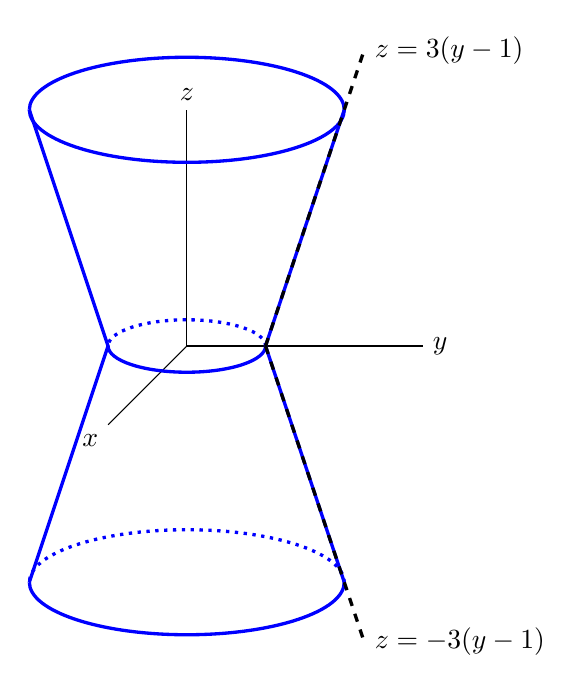
\begin{tikzpicture}
\draw (0,0)--(0,3)node[above]{$z$};
\draw (0,0)--(3,0) node[right]{$y$};
\draw (0,0)--(-1,-1) node[below left]{$x$};


\draw[very thick,blue] (1,0) arc (360:180:1cm and .333 cm);
\draw[dotted, very thick, blue] (1,0) arc (0:180:1cm and .333 cm);

\draw[very thick,blue] (2,3) arc (360:180:2cm and .667 cm);
\draw[very thick,blue] (2,3) arc (0:180:2cm and .667 cm);

\draw[very thick,blue] (2,-3,0) arc (360:180:2cm and .667 cm);
\draw[dotted, very thick, blue] (2,-3) arc (0:180:2cm and .667 cm);

\draw[very thick, blue] (2,-3)--(1,0)--(2,3) (-2,-3)--(-1,0)--(-2,3);

\draw[very thick, dashed] (1,0)--(2.25,3.75)node[right]{$z=3(y-1)$};
\draw[very thick, dashed] (1,0)--(2.25,-3.75)node[right]{$z=-3(y-1)$};

\end{tikzpicture}
\end{center}
\end{question}
\begin{hint}
Since the level curves are circles centred at the origin (in the $xy$-plane), the equation will have the form $x^2+y^2=g(z)$, where $g(z)$ is a function depending only on $z$.
\end{hint}
\begin{answer}
$\displaystyle x^2+y^2=\left( \frac{|z|}{3}+1\right)^2$
\end{answer}
\begin{solution}
Since the level curves are circles centred at the origin (in the $xy$-plane), when $z$ is a constant, the equation will have the form $x^2+y^2=c$ for some constant. That is, our equation looks like
\[x^2+y^2=g(z),\] where $g(z)$ is a function depending only on $z$.


Because our cross-sections are so nicely symmetric, we know the intersection of the figure with the left side of the $yz$-plane as well: $z=3(-y-1)=-3(y+1)$ 
(when $z\ge0$) and $z=-3(-y-1)=3(y+1)$ (when $z<0$). Below is the intersection of our surface with the $yz$ plane.

\begin{center}
\begin{tikzpicture}
\draw (0,-3)--(0,3)node[above]{$z$};
\draw (-3,0)--(3,0) node[right]{$y$};
%\draw (0,0)--(-1,-1) node[below left]{$x$};

\draw[very thick, dashed] (1,0)--(2.25,3.75)node[right]{$z=3(y-1)$};
\draw[very thick, dashed] (1,0)--(2.25,-3.75)node[right]{$z=-3(y-1)$};

\draw[very thick, dashed] (-1,0)--(-2.25,3.75)node[left]{$z=-3(y+1)$};
\draw[very thick, dashed] (-1,0)--(-2.25,-3.75)node[left]{$z=3(y+1)$};

\end{tikzpicture}
\end{center}

Setting $x=0$, our equation becomes $y^2=g(z)$. Looking at the right side of the $yz$ plane, this should lead to:
$\left.\begin{cases}
z=3(y-1) &\mbox{if } z\geq 0,\ y\ge 1\\
z=-3(y-1) &\mbox{if } z< 0,\ y\ge 1
\end{cases}\right\} $. That is:

\begin{align*}
|z|&=3(y-1)\\
\frac{|z|}{3}+1&=y\\
\left(\frac{|z|}{3}+1\right)^2&=y^2 &(*)
\end{align*}

A quick check: when we squared both sides of the equation in $(*)$, we added another solution, $\frac{|z|}{3}+1=-y$. Let's make sure we haven't diverged from our diagram.

\begin{align*}
&&& \left(\frac{|z|}{3}+1\right)^2=y^2\\
&\Leftrightarrow&& \underbrace{\frac{|z|}{3}+1}_{\text{positive}}=\pm y\\
&\Leftrightarrow&& \begin{cases}
 \frac{|z|}{3}+1 =y & y>0\\[0.05in]
  \frac{|z|}{3}+1 =-y & y<0
 \end{cases}\displaybreak[0]\\[0.1in]
& \Leftrightarrow&& \begin{cases}
 \frac{|z|}{3}+1 =y & y\ge1\\[0.05in]
  \frac{|z|}{3}+1 =-y & y\le-1
 \end{cases}\displaybreak[0]\\[0.1in]
&\Leftrightarrow&&  \begin{cases}
|z| =3(y-1) & y\ge1\\[0.05in]
|z|=-3(y+1) & y\le-1
 \end{cases}\displaybreak[0]\\[0.1in]
&\Leftrightarrow&&  \begin{cases}
z =\pm \underbrace{3(y-1)}_{\text{positive}} & y\ge1\\
z=\pm \underbrace{3(y+1)}_{\text{negative}} & y\le-1
 \end{cases}\displaybreak[0]\\[0.1in]
&\Leftrightarrow&&  \begin{cases}
z =3(y-1) & y\ge1,\ z\ge0\\
z =-3(y-1) & y\ge1,\ z\le0\\
z=-3(y+1) & y\le-1,\ z \ge 0\\
z=3(y+1) & y\le-1,\ z\le 0
 \end{cases}
\end{align*}

This matches our diagram eactly. So, all together, the equation of the surface is
\[x^2+y^2=\left( \frac{|z|}{3}+1\right)^2\]
\end{solution}
%%%%%%%%%%%%%%%%%%%

%\section{Cylinders}
%\input{prob_s1.8}
%\section{Quadric Surfaces}
%\input{prob_s1.9}

%%%%%%%%%%%%%%%%%%%%%%%%%%%%%%%%%%%%%
\chapter{Partial Derivatives}
\section{Limits}
%\documentclass[12pt]{article}

\questionheader{ex:s2.1}


%%%%%%%%%%%%%%%%%%
\subsection*{\Conceptual}
%%%%%%%%%%%%%%%%%%
%%%%%%%%%%%%%%%%%%%
%%%%%%%%%%%%%%%%%%%
\begin{question}
Suppose $f(x,y)$ is a function such that 
         $\lim\limits_{(x,y)\to(0,0)}f(x,y)=10$. 

True or false: $|f(0.1,0.1)-10|<|f(0.2,0.2)-10|$
\end{question}
\begin{hint}
How does the behaviour of a function far away from $(0,0)$ affect its limit at $(0,0)$?
\end{hint}
\begin{answer}
in general, false.
\end{answer}
\begin{solution}
In general, this is false. Consider $f(x,y)=12-(1-10x)^2-(1-10y)^2$. 
\begin{itemize}
\item $\lim\limits_{(x,y)\to(0,0)}f(x,y)=12-1-1=10$ (the function is continuous)
\item $f(0.1,0.1)=12-(1-1)^2-(1-1)^2=12$
\item $f(0.2,0.2)=12-(1-2)^2-(1-2)^2=10$
\end{itemize}

We often (somewhat lazily) interpret the limit\quad ``$\lim\limits_{(x,y)\to(0,0)}f(x,y)=10$" \quad to mean that, as $(x,y)$ gets 
closer and closer to the origin, $f(x,y)$ gets closer and closer to 10. This 
isn't exactly what the definition means, though. The definition tells us that, 
we can guarantee that $f(x,y)$ be very close to 10 by choosing 
$(x,y)$ very close to $(0,0)$.

The function $f(x,y)$ can also be very close to 10 for some $(x,y)$'s that are not close to $(0,0)$. Moreover, we don't know \emph{how close} to $(0,0)$ 
we have to be in order for $f(x,y)$ to be ``very close" to 10.
\end{solution}
%%%%%%%%%%%%%%%%%%%
%%%%%%%%%%%%%%%%%%%

\begin{question}
A millstone pounds wheat into flour. The wheat sits in a basin, and the millstone pounds up and down.

Samples of wheat are taken from various places along the basin. Their diameters are measured and their position on the basin is recorded.

Consider this claim: ``As the particles get very close to the millstone, the diameters of the particles approach 50 $\mu$m."
In this context, describe the variables below from Definition~\eref{CLP200}{def limit} in the CLP-3 text.

\begin{enumerate}[(a)]
\item $\mathbf x$
\item $\mathbf a$
\item $\mathbf L$
\end{enumerate}
\end{question}
\begin{hint}
In this analogy, $f(x,y)$ is the diameter of a particle taken from the position $(x,y)$ in the basin.
\end{hint}
\begin{answer}
(a) the position of the particle in the basin \\
(b) the position in the basin that the millstone hits\\
(c) 50 $\mu$m
\end{answer}
\begin{solution}

\begin{enumerate}[(a)]
\item The function we're taking the limit of has its input as the position of the particle, and its output the size of the particle. So, $f(x,y)$ gives the size of particles found at position $(x,y)$. In the definition, we write $\mathbf x = (x,y)$. So, $\mathbf x$ is the position in the basin the particle was taken from.
\item Our claim deals with particles very close to where the millstone hits the basin, so $\mathbf a$ is the position in the basinfwhere the millstone hits.
\item $\mathbf L$ is the limit of the function: in this case, 50 $\mu$m.
\end{enumerate}

\end{solution}
%%%%%%%%%%%%%%%%%%%
%%%%%%%%%%%%%%%%%%%

\begin{question}
Let $f(x,y)=\dfrac{x^2}{x^2+y^2}$.
\begin{enumerate}[(a)]
\item Find a ray approaching the origin along which $f(x,y)=1$.
\item Find a ray approaching the origin along which $f(x,y)=0$.
\item What does the above work show about a limit of $f(x,y)$?
\end{enumerate}
\end{question}
\begin{hint}
You can probably solve (a) and (b) by just staring at $f(x,y)$.
\end{hint}
\begin{answer}
(a) along the $x$-axis\qquad (b) along the $y$-axis \qquad (c) $\lim\limits_{(x,y)\to(0,0)}f(x,y)$ does not exist
\end{answer}
\begin{solution}
\begin{enumerate}[(a)]
\item By inspection, when $y=0$, then $f(x,y)=1$ as long as $x \neq 0$. So, if we follow the $x$-axis in towards the origin, $f(x,y)=1$ along this route.
\item Also by inspection, when $x=0$, then $f(x,y)=0$ as long as $y \neq 0$. So, if we follow the $y$-axis in towards the origin, $f(x,y)=0$ along this route.
\item Since two different directions give us different values as we approach the origin,  $\lim\limits_{(x,y)\to(0,0)}f(x,y)$ does not exist.
\begin{center}
\begin{tikzpicture}
\YEaxis{1.5}{1.5}
\draw[very thick,<-,dashed] (0,.2)--(0,1) node[above left]{$f=0$};
\draw[very thick,<-,dashed] (0,-.2)--(0,-1) node[below right]{$f=0$};
\draw[thick,<-] (.2,0)--(1,0) node[above right]{$f=1$};
\draw[thick,<-] (-0.2,0)--(-1,0) node[below left]{$f=1$};
\end{tikzpicture}
\end{center}
\end{enumerate}

\end{solution}
%%%%%%%%%%%%%%%%%%%
%%%%%%%%%%%%%%%%%%%
\begin{question}
Let $f(x,y)=x^2-y^2$
\begin{enumerate}[(a)]
\item Express the function in terms of the polar coordinates $r$ and $\theta$, and simplify.
\item Suppose $(x,y)$ is a distance of 1 from the origin. 
What are the largest and smallest values of $f(x,y)$?
\item Let $r>0$. Suppose $(x,y)$ is a distance of $r$ from the origin. 
What are the largest and smallest values of $f(x,y)$?
\item Let $\epsilon>0$. Find a positive value of $r$ that guarantees $|f(x,y)|<\epsilon$ whenever $(x,y)$ is at most $r$ units from the origin.
\item What did you just show?
\end{enumerate}
\end{question}
\begin{hint}
Recall $\cos^2\theta-\sin^2\theta=\cos(2\theta)$
\end{hint}
\begin{answer}
(a) $r^2\cos(2\theta)$\quad 
(b) $\text{min}=-1,\ \text{max}=1$\quad 
(c) $\text{min}=-r^2,\ \text{max}=r^2$\quad 
(d) $r<\sqrt\epsilon$ 

(e) $\lim\limits_{(x,y)\to(0,0)}f(x,y)=0$

\end{answer}
\begin{solution}
\begin{enumerate}[(a)]
\item Since $x=r\cos\theta$ and $y=r\sin\theta$, we have that 
\begin{equation*}
f=x^2-y^2=r^2\cos^2\theta-r^2\sin^2\theta=r^2\cos(2\theta)
\end{equation*}
\item 
When $r=1$, $f=\cos(2\theta)$. So, $f(x,y)$ runs between $-1$ and $1$.
It smallest value is $-1$ and its largest value is $+1$.
\item 
The distance from $(x,y)$ to the origin is $r$ (for $r\ge0)$. So, at a distance $r$, our function is $r^2\cos(2\theta)$. Then $f(x,y)$ runs over the interval $[-r^2,r^2]$. It smallest value is $-r^2$ and its largest value is $+r^2$.
\item 
Using our answer to the last part, we have that $|f|\le r^2$. So for $0<r<\sqrt\epsilon$, we necessarily have that $|f(x,y)|<\epsilon$ 
whenever the distance from $(x,y)$ to the origin is at most $r$.
\item 
For every $\epsilon>0$, if we choose $(x,y)$ to be sufficiently close to $(0,0)$ (in particular, within a distance $r<\sqrt\epsilon$), then $f(x,y)$ is 
within distance $\epsilon$ of $0$. By Definition~\eref{CLP200}{def limit} 
in the CLP-3 text, we have that $\lim\limits_{(x,y)\to(0,0)}f(x,y)=0$.
\end{enumerate}

\end{solution}
%%%%%%%%%%%%%%%%%%%
%%%%%%%%%%%%%%%%%%%
\begin{question}
Suppose $f(x,y)$ is a polynomial. Evaluate $\lim\limits_{(x,y)\to(a,b)}f(x,y)$, where $(a,b)\in\mathbb R^2$.
\end{question}
\begin{hint}
Theorem~\eref{CLP200}{thm one d continuity}%2.1.6
in the CLP-3 text
\end{hint}
\begin{answer}
$f(a,b)$
\end{answer}
\begin{solution}
By Theorem~\eref{CLP200}{thm one d continuity},%2.1.6 
$f(x,y)$ is continuous over its domain. The domain of a polynomial is everywhere; in this case, $\mathbb R^2$. So, $f(x,y)$ is continuous at $(a,b)$. By the definition of continuity, $\lim\limits_{(x,y)\to(a,b)}f(x,y)=f(a,b)$.
\end{solution}
%%%%%%%%%%%%%%%%%%%
%%%%%%%%%%%%%%%%%%
\subsection*{\Procedural}
%%%%%%%%%%%%%%%%%%

%%%%%%%%%%%%%%%%%%%%%%%%%%%%%%%%
\begin{question}
Evaluate, if possible,
\begin{enumerate}[(a)]
\item $\dst\lim_{(x,y)\rightarrow(2,-1)}\ \big(xy+x^2\big)$
\item $\dst\lim_{(x,y)\rightarrow(0,0)}\ \frac{x}{x^2+y^2}$
\item $\dst\lim_{(x,y)\rightarrow(0,0)}\ \frac{x^2}{x^2+y^2}$
\item $\dst\lim_{(x,y)\rightarrow(0,0)}\ \frac{x^3}{x^2+y^2}$
\item $\dst\lim_{(x,y)\rightarrow(0,0)}\ \frac{x^2y^2}{x^2+y^4}$
\item $\dst\lim_{(x,y)\rightarrow (0,0)}\ 
                        \frac{(\sin x)\left(e^y-1\right)}{xy}$
\end{enumerate}
\end{question}

\begin{hint}
For parts (b), (c), (d), (e), switch to polar coordinates.
For part (f),
\begin{equation*} 
\lim_{(x,y)\rightarrow (0,0)}\ 
                        \frac{(\sin x)\left(e^y-1\right)}{xy}
=\left[\lim_{x\rightarrow 0}\ 
                        \frac{\sin x}{x}\right]\ 
 \left[\lim_{y\rightarrow 0}\ 
                        \frac{e^y-1}{y}\right]
\end{equation*}
\end{hint}

\begin{answer}
(a) $2$ \qquad
(b) undefined\qquad
(c) undefined\qquad
(d) $0$\qquad
(e) $0$ \qquad
(f) $1$
\end{answer}

\begin{solution}
(a) $\dst\lim_{(x,y)\rightarrow(2,-1)}\ \big(xy+x^2\big)=2(-1)+2^2=2$

(b) Switching to polar coordinates,
\begin{align*}
\lim_{(x,y)\rightarrow(0,0)}\ \frac{x}{x^2+y^2}
    &=\lim_{\Atop{r\rightarrow0^+}{0\le\theta<2\pi}}\ \frac{r\cos\theta}{r^2}
     =\lim_{\Atop{r\rightarrow0^+}{0\le\theta<2\pi}}\ \frac{\cos\theta}{r} 
\end{align*}
which does not exist, since, for example,
\begin{itemize}
\item 
if $\theta=0$, then 
\begin{equation*}
\lim_{\Atop{r\rightarrow0^+}{\theta=0}}\ \frac{\cos\theta}{r}
=\lim_{r\rightarrow0^+}\ \frac{1}{r}
=+\infty
\end{equation*}
\item
while if $\theta=\pi$, then 
\begin{equation*}
\lim_{\Atop{r\rightarrow0^+}{\theta=\pi}}\ \frac{\cos\theta}{r}
=\lim_{r\rightarrow0^+}\ \frac{-1}{r}
=-\infty
\end{equation*}
\end{itemize}

(c) Switching to polar coordinates,
\begin{align*}
\lim_{(x,y)\rightarrow(0,0)}\ \frac{x^2}{x^2+y^2}
  &=\lim_{\Atop{r\rightarrow0^+}{0\le\theta<2\pi}}\ \frac{r^2\cos^2\theta}{r^2}
     =\lim_{\Atop{r\rightarrow0^+}{0\le\theta<2\pi}}\ \cos^2\theta 
\end{align*}
which does not exist, since, for example,
\begin{itemize}
\item 
if $\theta=0$, then 
\begin{equation*}
\lim_{\Atop{r\rightarrow0^+}{\theta=0}}\ \cos^2\theta
=\lim_{r\rightarrow0^+}\ 1
= 1
\end{equation*}
\item
while if $\theta=\frac{\pi}{2}$, then 
\begin{equation*}
\lim_{\Atop{r\rightarrow0^+}{\theta=\pi/2}}\ \cos^2\theta
=\lim_{r\rightarrow0^+}\ 0
=0
\end{equation*}
\end{itemize}

(d) Switching to polar coordinates,
\begin{align*}
\lim_{(x,y)\rightarrow(0,0)}\ \frac{x^3}{x^2+y^2}
   &=\lim_{\Atop{r\rightarrow0^+}{0\le\theta<2\pi}}\ \frac{r^3\cos^3\theta}{r^2}
     =\lim_{\Atop{r\rightarrow0^+}{0\le\theta<2\pi}}\ r\cos^3\theta 
    =0
\end{align*}
since $|\cos\theta|\le 1$ for all $\theta$.

(e) Switching to polar coordinates,
\begin{align*}
    \lim_{(x,y)\rightarrow(0,0)}\ \frac{x^2y^2}{x^2+y^4}
    &=\lim_{\Atop{r\rightarrow0^+}{0\le\theta<2\pi}}\ 
                                \frac{r^2\cos^2\theta\ r^2\sin^2\theta}
                                      {r^2\cos^2\theta+r^4\sin^4\theta}
   =\lim_{\Atop{r\rightarrow0^+}{0\le\theta<2\pi}}\ r^2\sin^2\theta
                  \frac{\cos^2\theta}{\cos^2\theta+r^2\sin^4\theta} \\
   &=  0
\end{align*} 
Here, we used that 
\begin{equation*}
\left|\sin^2\theta\frac{\cos^2\theta} {\cos^2\theta+r^2\sin^4\theta}\right|
\le \frac{\cos^2\theta} {\cos^2\theta+r^2\sin^4\theta}
\le \left.\begin{cases}
             \frac{\cos^2\theta} {\cos^2\theta}&\text{ if }\cos\theta\ne 0 \\
              0 &\text { if }\cos\theta =0
           \end{cases}
     \right\}
\le 1
\end{equation*} 
for all $r>0$.

(f) To start, observe that
\begin{align*}
\lim_{(x,y)\rightarrow (0,0)}\ 
                  \frac{(\sin x)\left(e^y-1\right)}{xy}
          =\left[\lim_{x\rightarrow 0}\ 
                  \frac{\sin x}{x}\right]
            \left[\lim_{y\rightarrow 0}\ 
                  \frac{e^y-1}{y}\right]
\end{align*}
We may evaluate  $\dst\left[\lim_{x\rightarrow 0}\ 
                  \frac{\sin x}{x}\right]$
by l'H\^opital's rule or by using the definition of the derivative to give
\begin{equation*}
\lim_{x\rightarrow 0}\ \frac{\sin x}{x}
=\lim_{x\rightarrow 0}\ \frac{\sin x-\sin 0}{x-0}
=\diff{}{x}\sin x\bigg|_{x=0}
=\cos x\Big|_{x=0}=1
\end{equation*}
Similarly, we may evaluate  $\dst\left[\lim_{y\rightarrow 0}\ 
                  \frac{e^y-1}{y}\right]$
by l'H\^opital's rule or by using the definition of the derivative to give
\begin{equation*}
\lim_{y\rightarrow 0}\ \frac{e^y-1}{y}
=\lim_{y\rightarrow 0}\ \frac{e^y-e^0}{y-0}
=\diff{}{y}e^y\bigg|_{y=0}
=e^y\Big|_{y=0}=1
\end{equation*}
So all together
\begin{align*}
\lim_{(x,y)\rightarrow (0,0)}\ 
                  \frac{(\sin x)\left(e^y-1\right)}{xy}
          =\left[\lim_{x\rightarrow 0}\ 
                  \frac{\sin x}{x}\right]
            \left[\lim_{y\rightarrow 0}\ 
                  \frac{e^y-1}{y}\right]
          =[1]\ [1]=1
\end{align*}
\end{solution}

%%%%%%%%%%%%%%%%%%%%%%%%%%%%%%%%
\begin{question}[M253 2009D] %8
\begin{enumerate}[(a)]
\item
Find the limit: $\dst \lim_{(x,y)\to(0,0)}\frac{x^8+y^8}{x^4+y^4}$.
\item
Prove that the following limit does not exist: 
  $\dst \lim_{(x,y)\to(0,0)}\frac{xy^5}{x^8+y^{10}}$.
\end{enumerate}
\end{question}

\begin{hint}
Switch to polar coordinates.
\end{hint}

\begin{answer}
(a) $0$
\qquad
(b) See the solution.
\end{answer}

\begin{solution}
(a)
In polar coordinates, $x=r\cos\theta$, $y=r\sin\theta$, so that 
\begin{align*}
\frac{x^8+y^8}{x^4+y^4}
&=\frac{r^8\cos^8\theta+r^8\sin^8\theta}{r^4\cos^4\theta+r^4\sin^4\theta}
=r^4\frac{\cos^8\theta+\sin^8\theta}{\cos^4\theta+\sin^4\theta}
\end{align*}
As
\begin{align*}
\frac{\cos^8\theta+\sin^8\theta}{\cos^4\theta+\sin^4\theta}
&\le \frac{\cos^8\theta+2\cos^4\theta\sin^4\theta+\sin^8\theta}
             {\cos^4\theta+\sin^4\theta}
=\frac{\big(\cos^4\theta+\sin^4\theta\big)^2}{\cos^4\theta+\sin^4\theta} \\
&=\cos^4\theta+\sin^4\theta
%\le\cos^2\theta+\sin^2\theta=1
\le 2
\end{align*}
we have
\begin{equation*}
0\le \frac{x^8+y^8}{x^4+y^4}\le 2r^4
\end{equation*}
As $\dst\lim_{(x,y)\to (0,0)}2r^4=0$, the squeeze theorem yields
 $\dst\lim_{(x,y)\to(0,0)}\frac{x^8+y^8}{x^4+y^4}=0$.

(b)  
In polar coordinates
\begin{align*}
\frac{xy^5}{x^8+y^{10}}
&=\frac{r^6\cos\theta\,\sin^5\theta}{r^8\cos^8\theta+r^{10}\sin^{10}\theta}
=\frac{1}{r^2}\frac{\cos\theta\,\sin^5\theta}{\cos^8\theta+r^2\sin^{10}\theta}
\end{align*}
As $(x,y)\to (0,0)$ the first fraction $\frac{1}{r^2}\to\infty$ but the second
factor can take many different values. For example, if we send $(x,y)$
towards the origin along the $y$--axis, i.e. with 
$\theta=\pm\frac{\pi}{2}$,
\begin{align*}
\lim_{\Atop {(x,y)\to(0,0)}{x=0}}\frac{xy^5}{x^8+y^{10}}
=\lim_{y\to 0} \frac{0}{y^{10}}=0
\end{align*} 
but if we send $(x,y)$ towards the origin along the line $y=x$, 
i.e. with  $\theta=\frac{\pi}{4},\frac{5\pi}{4}$,
\begin{align*}
\lim_{\Atop {(x,y)\to(0,0)}{y=x} }\frac{xy^5}{x^8+y^{10}}
=\lim_{x\to 0} \frac{x^6}{x^8+x^{10}}
=\lim_{x\to 0} \frac{1}{x^2}\frac{1}{1+x^2}
=+\infty
\end{align*} 
and if we send $(x,y)$ towards the origin along the line $y=-x$, 
i.e. with  $\theta=-\frac{\pi}{4},\frac{3\pi}{4}$,
\begin{align*}
\lim_{\Atop {(x,y)\to(0,0)}{y=-x} }\frac{xy^5}{x^8+y^{10}}
=\lim_{x\to 0} \frac{-x^6}{x^8+x^{10}}
=\lim_{x\to 0}- \frac{1}{x^2}\frac{1}{1+x^2}
=-\infty
\end{align*} 
So $\frac{xy^5}{x^8+y^{10}}$ does not approach a single value as 
$(x,y)\to(0,0)$ and the limit does not exist.

\end{solution}

%%%%%%%%%%%%%%%%%%%%%%%%%%%%%%%%
\begin{question}[M2226 2009D] %7
Evaluate each of the following limits or show that it does not exist.
\begin{enumerate}[(a)]
\item
$\dst\lim_{(x,y)\rightarrow (0,0)}\frac{x^3-y^3}{x^2+y^2}$
\item
$\dst\lim_{(x,y)\rightarrow (0,0)}\frac{x^2-y^4}{x^2+y^4}$
\end{enumerate}
\end{question}

\begin{hint}
(a) Switch to polar coordinates.

(b) What are the limits when (i) $x=0$ and $y\rightarrow 0$ and when
(ii) $y=0$ and $x\rightarrow 0$?
\end{hint}

\begin{answer}
(a) $0$

(b) The limit does not exist since the limits (i) $x=0$,
$y\rightarrow 0$ and (ii) $y=0$, $x\rightarrow 0$ are different.
\end{answer}

\begin{solution}
(a) In polar coordinates
\begin{equation*}
\frac{x^3-y^3}{x^2+y^2}=\frac{r^3\cos^3\theta-r^3\sin^3\theta}{r^2}
=r\cos^3\theta-r\sin^3\theta
\end{equation*}
Since
\begin{equation*}
\big|r\cos^3\theta-r\sin^3\theta\big|\le 2r
\end{equation*}
and $2r\rightarrow 0$ as $r\rightarrow 0$, the limit exists and is $0$.

(b)
The limit as we approach $(0,0)$ along the $x$-axis is
\begin{align*}
\lim_{t\rightarrow 0}\frac{x^2-y^4}{x^2+y^4}\bigg|_{(x,y)=(t,0)}
=\lim_{t\rightarrow 0}\frac{t^2-0^4}{t^2+0^4}
=1
\end{align*}
On the other hand the limit as we approach $(0,0)$ along the $y$-axis is
\begin{align*}
\lim_{t\rightarrow 0}\frac{x^2-y^4}{x^2+y^4}\bigg|_{(x,y)=(0,t)}
=\lim_{t\rightarrow 0}\frac{0^2-t^4}{0^2+t^4}
=-1
\end{align*}
These are different, so the limit as $(x,y)\rightarrow 0$ does not exist.

We can gain a more detailed understanding of the behaviour of 
$\frac{x^2-y^4}{x^2+y^4}$ near the origin by switching to polar coordinates.
\begin{equation*}
\frac{x^2-y^4}{x^2+y^4}
=\frac{r^2\cos^2\theta-r^4\sin^4\theta}{r^2\cos^2\theta+r^4\sin^4\theta}
=\frac{\cos^2\theta-r^2\sin^4\theta}{\cos^2\theta+r^2\sin^4\theta}
\end{equation*}
Now fix any $\theta$ and let $r\rightarrow 0$ (so that we are approaching the origin along the ray that makes an angle $\theta$ with the positive $x$-axis).
If $\cos\theta\ne 0$ (i.e. the ray is not part of the $y$-axis)
\begin{align*}
\lim_{r\rightarrow 0}
     \frac{\cos^2\theta-r^2\sin^4\theta}{\cos^2\theta+r^2\sin^4\theta}
=\frac{\cos^2\theta}{\cos^2\theta}
=1
\end{align*}
But if $\cos\theta= 0$ (i.e. the ray is part of the $y$-axis)
\begin{align*}
\lim_{r\rightarrow 0}
     \frac{\cos^2\theta-r^2\sin^4\theta}{\cos^2\theta+r^2\sin^4\theta}
=\lim_{r\rightarrow 0}
     \frac{-r^2\sin^4\theta}{r^2\sin^4\theta}
=\frac{-\sin^4\theta}{\sin^4\theta}
=-1
\end{align*}
\end{solution}

%%%%%%%%%%%%%%%%%%
\subsection*{\Application}
%%%%%%%%%%%%%%%%%%

%%%%%%%%%%%%%%%%%%%%%%%%%%%%%%%%
\begin{question}[M226 2010D] %6
Evaluate each of the following limits or show that it does not exist.
\begin{enumerate}[(a)]
\item
$\dst\lim_{(x,y)\rightarrow (0,0)}\frac{2x^2 + x^2y - y^2x + 2y^2}{x^2 + y^2}$
\item
$\dst\lim_{(x,y)\rightarrow(0,1)} \frac{x^2y^2 -2 x^2y + x^2}
                                       {(x^2 + y^2-2y+1)^2}$
\end{enumerate}
\end{question}

\begin{hint}
For part (a) switch to polar coordinates.
For part (b), switch to polar coordinates
centred on $(0,1)$. That is, make the change of variables
$x=r\cos\theta$, $y=1+r\sin\theta$. 
\end{hint}

\begin{answer}
(a) $2$\qquad
(b) The limit does not exist. See the solution.
\end{answer}

\begin{solution}
(a) In polar coordinates $x=r\cos\theta$, $y=r\sin\theta$
\begin{align*}
\frac{2x^2 + x^2y - y^2x + 2y^2}{x^2 + y^2} 
&=\frac{2r^2\cos^2\theta + r^3\cos^2\theta\sin\theta - r^3\cos\theta\sin^2\theta 
                 + 2r^2\sin^2\theta}{r^2} \\ 
&=2+ r\big[\cos^2\theta\sin\theta - \sin^2\theta\cos\theta \big]
\end{align*}
As
\begin{equation*}
r\big|\cos^2\theta\sin\theta - \sin^2\theta\cos\theta \big|
\le 2r
\rightarrow 0\text{ as }r\rightarrow 0
\end{equation*}
we have
\begin{equation*}
\lim_{(x,y)\rightarrow(0,0)} \frac{2x^2 + x^2y - y^2x + 2y^2}{x^2 + y^2}=2
\end{equation*}

(b)
Since 
\begin{align*}
\frac{x^2y^2 -2 x^2y + x^2} {(x^2 + y^2-2y+1)^2} 
=\frac{x^2(y-1)^2} {\big[x^2 + (y-1)^2\big]^2} 
\end{align*}
and, in polar coordinates centred on $(0,1)$,
$x=r\cos\theta$, $y=1+r\sin\theta$,
\begin{equation*}
\frac{x^2(y-1)^2} {\big[x^2 + (y-1)^2\big]^2} 
=\frac{r^4\cos^2\theta\sin^2\theta}{r^4}
=\cos^2\theta\sin^2\theta
\end{equation*}
we have that the limit does not exist. For example, if we send $(x,y)$
to $(0,1)$ along the line $y=1$, so that $\theta=0$, we get the limit $0$,
while if we send $(x,y)$ to $(0,1)$ along the line $y=x+1$, so that 
$\theta=\frac{\pi}{4}$, we get the limit $\frac{1}{4}$.
\end{solution}

%%%%%%%%%%%%%%%%%%%%%%%%%%%%%%%%
\begin{question}
Define, for all $(x,y)\ne(0,0)$, $f(x,y)=\frac{x^2y}{x^4+y^2}$.
\begin{enumerate}[(a)]
\item
Let $0\le \theta<2\pi$. Compute
$\dst\lim_{r\rightarrow 0^+}f(r\cos\theta,r\sin\theta)$.

\item 
Compute $\dst\lim_{x\rightarrow 0}f(x,x^2)$.

\item
Does $\dst\lim_{(x,y)\rightarrow (0,0)}f(x,y)$ exist?
\end{enumerate}
\end{question}

\begin{hint}
For part (c), does there exist a single number, $L$, with the property that
$f(x,y)$ is really close to $L$ for all $(x,y)$ that are really close to 
$(0,0)$?
\end{hint}

\begin{answer}
(a) $0$\qquad
(b) $\frac{1}{2}$ \qquad
(c) No.
\end{answer}

\begin{solution}
(a) We have
\begin{align*}
\lim_{r\rightarrow 0^+}f(r\cos\theta,r\sin\theta)
&=\lim_{r\rightarrow 0^+}
\frac{(r\cos\theta)^2(r\sin\theta)}{(r\cos\theta)^4+(r\sin\theta)^2} \\
&=\lim_{r\rightarrow 0^+}r\ \frac{\cos^2\theta\sin\theta}{r^2\cos^4\theta+\sin^2\theta} \\
&=\lim_{r\rightarrow 0^+}r\ 
\lim_{r\rightarrow 0^+}\frac{\cos^2\theta\sin\theta}
                         {r^2\cos^4\theta+\sin^2\theta}
\end{align*}
Observe that, if $\sin\theta=0$, then
\begin{equation*}
\frac{\cos^2\theta\sin\theta}{r^2\cos^4\theta+\sin^2\theta}=0
\end{equation*}
for all $r\ne 0$. If $\sin\theta\ne 0$,
\begin{align*}
\lim_{r\rightarrow 0^+}   
     \frac{\cos^2\theta\sin\theta}{r^2\cos^4\theta+\sin^2\theta}
&=\frac{\cos^2\theta\sin\theta}{\sin^2\theta}
=\frac{\cos^2\theta}{\sin\theta}
\end{align*}
So the limit 
$\dst\lim_{r\rightarrow 0^+}
\frac{\cos^2\theta\sin\theta}{r^2\cos^4\theta+\sin^2\theta}$
exists (and is finite) for all fixed $\theta$ and 
\begin{equation*}
\lim\limits_{r\rightarrow 0^+}f(r\cos\theta,r\sin\theta)=0
\end{equation*}

(b) We have
\begin{equation*}
\lim_{x\rightarrow 0}f(x,x^2)
=\lim_{x\rightarrow 0}\frac{x^2x^2}{x^4+{(x^2)}^2}
=\lim_{x\rightarrow 0}\frac{x^4}{2x^4}
=\frac{1}{2}
\end{equation*}

(c)
Note that in part (a) we showed that as $(x,y)$ approaches $(0,0)$ along
any straight line, $f(x,y)$ approaches the limit zero.
In part (b) we have just shown that as $(x,y)$ approaches $(0,0)$ along
the parabola $y=x^2$, $f(x,y)$ approaches the limit $\half$, {\bf not} zero.
So $f(x,y)$ takes values very close to $0$, for some $(x,y)$'s 
that are  really near $(0,0)$ and also takes values very close to 
$\frac{1}{2}$, for other $(x,y)$'s that are  really near $(0,0)$.
There is no single number, $L$, with the property that
$f(x,y)$ is really close to $L$ for all $(x,y)$ that are really 
close to $(0,0)$. So the limit does not exist.

\end{solution}

%%%%%%%%%%%%%%%%%%%%%%%%%%%%%%%%
\begin{question}[M226 2007D] %1
Compute the following limits or explain why they do not exist.
\begin{enumerate}[(a)]
\item $\dst\lim_{(x,y)\rightarrow(0,0)}\frac{xy}{x^2+y^2}$
\item $\dst\lim_{(x,y)\rightarrow(0,0)}\frac{\sin(xy)}{x^2+y^2}$
\item $\dst\lim_{(x,y)\rightarrow(-1,1)}\frac{x^2+2xy^2+y^4}{1+y^4}$
\item $\dst\lim_{(x,y)\rightarrow(0,0)}|y|^x$
\end{enumerate}
\end{question}

\begin{hint}
For part (b), consider the ratio of $\frac{\sin(xy)}{x^2+y^2}$
(from part (b)) and $\frac{xy}{x^2+y^2}$ (from part (a)), and recall that
$\dst\lim_{t\rightarrow 0}\tfrac{\sin t}{t}=1$.

For part (d) consider the limits along the positive $x$- and $y$-axes.
\end{hint}

\begin{answer}
(a), (b), (d) Do not exist. See the solutions.\qquad
(c) $0$
\end{answer}

\begin{solution}
(a) Since, in polar coordinates,
\begin{equation*}
\frac{xy}{x^2+y^2}=\frac{r^2\cos\theta\sin\theta}{r^2}
=\cos\theta\sin\theta
\end{equation*}
we have that the limit does not exist. For example, 
\begin{itemize}
\item if we send $(x,y)$
to $(0,0)$ along the positive $x$-axis, so that $\theta=0$, 
we get the limit $\sin\theta\cos\theta\big|_{\theta=0}=0$, 
\item
while if we send $(x,y)$ to $(0,0)$ along the line $y=x$ in the first quadrant, 
so that  $\theta=\frac{\pi}{4}$, we get the limit $\sin\theta\cos\theta\big|_{\theta=\pi/4}=\frac{1}{2}$.
\end{itemize}

(b) This limit does not exist, since if it were to exist the limit
\begin{equation*}
\lim_{(x,y)\rightarrow(0,0)}\frac{xy}{x^2+y^2}
=\lim_{(x,y)\rightarrow(0,0)}\frac{xy}{\sin(xy)}\ \frac{\sin(xy)}{x^2+y^2}
=\lim_{(x,y)\rightarrow(0,0)}\frac{xy}{\sin(xy)}\ 
\lim_{(x,y)\rightarrow(0,0)}\frac{\sin(xy)}{x^2+y^2}
\end{equation*}
would also exist. (Recall that $\dst\lim_{t\rightarrow 0}\tfrac{\sin t}{t}
=1$.)


(c) Since
\begin{align*}
\lim_{(x,y)\rightarrow(-1,1)}\big[x^2+2xy^2+y^4\big]
&=(-1)^2+2(-1)(1)^2+(1)^4=0 \\
\lim_{(x,y)\rightarrow(-1,1)}\big[1+y^4\big]
&=1+(1)^4=2
\end{align*}
and the second limit is nonzero,
\begin{equation*}
\lim_{(x,y)\rightarrow(-1,1)}\frac{x^2+2xy^2+y^4}{1+y^4}=\frac{0}{2}=0
\end{equation*}




(d)  Since the limit along the positive $x$-axis
\begin{equation*}
\lim_{\Atop{t\rightarrow 0}{t>0}}|y|^x\Big|_{(x,y)=(t,0)}
=\lim_{\Atop{t\rightarrow 0}{t>0}}0^t
=\lim_{\Atop{t\rightarrow 0}{t>0}}0
=0
\end{equation*}
and the limit along the $y$-axis
\begin{equation*}
\lim_{t\rightarrow 0}|y|^x\Big|_{(x,y)=(0,t)}
=\lim_{t\rightarrow 0}|t|^0
=\lim_{t\rightarrow 0}1
=1
\end{equation*}
are different, the limit as $(x,y)\rightarrow 0$ does not exist.
\end{solution}

%%%%%%%%%%%%%%%%%%%%%%%%%%%%%%%%
\begin{question}
Evaluate each of the following limits or show that it does not exist.
\begin{enumerate}[(a)]
\item
$\dst\lim_{(x,y)\rightarrow (0,0)}\begin{cases}
                                   \frac{x^2}{y-x} &\text{if $y\ne x$} \\
                                   0 & \text{if $y=x$}
                                   \end{cases}
$
\item
$\dst\lim_{(x,y)\rightarrow(0,0)}\begin{cases}
                                   \frac{x^8}{y-x} &\text{if $y\ne x$} \\
                                   0 & \text{if $y=x$}
                                   \end{cases}
$
\end{enumerate}
\end{question}

\begin{hint}
For part (a), determine what happens as $(x,y)$ tends to $(0,0)$
along the curve $y=x+\frac{x^2}{a}$, where $a$ is any nonzero constant.

\end{hint}

\begin{answer}
(a), (b)  The limit does not exist. See the solution.
\end{answer}

\begin{solution}
(a) Let $a$ be any nonzero constant. When $y=x+\frac{x^2}{a}$ and $x\ne 0$,
\begin{equation*}
\frac{x^2}{y-x} =\frac{x^2}{x^2/a} =a
\end{equation*}
So the limit along the curve $y=x+\frac{x^2}{a}$ is
\begin{equation*}
\lim_{t\rightarrow 0}\frac{x^2}{y-x}\Big|_{(x,y)=(t,t+t^2/a)}
=\lim_{t\rightarrow 0}a
=a
\end{equation*}
In particular, the limit along the curve $y=x+x^2$, which is $1$, and 
the limit along the curve $y=x-x^2$, which is $-1$, are different.
So the limit as $(x,y)\rightarrow 0$ does not exist.

(b) Let $a$ be any nonzero constant. When $y=x+\frac{x^8}{a}$ and $x\ne 0$,
\begin{equation*}
\frac{x^8}{y-x} =\frac{x^8}{x^8/a} =a
\end{equation*}
So the limit along the curve $y=x+\frac{x^8}{a}$ is
\begin{equation*}
\lim_{t\rightarrow 0}\frac{x^8}{y-x}\Big|_{(x,y)=(t,t+t^8/a)}
=\lim_{t\rightarrow 0}a
=a
\end{equation*}
In particular, the limit along the curve $y=x+x^8$, which is $1$, and 
the limit along the curve $y=x-x^8$, which is $-1$, are different.
So the limit as $(x,y)\rightarrow 0$ does not exist.
\end{solution}


\section{Partial Derivatives}
%\documentclass[12pt]{article}

\questionheader{ex:s2.2}


%%%%%%%%%%%%%%%%%%
\subsection*{\Conceptual}
%%%%%%%%%%%%%%%%%%

%%%%%%%%%%%%%%%%%%%%%%%%%%%%%%%%
\begin{question}
Let $f(x,y) = e^x\cos y$. The following table gives some values of $f(x,y)$.

\begin{center}
\renewcommand{\arraystretch}{1.3}
     \begin{tabular}{c|c|c|c|}
       & $x=0$ & $x=0.01$ & $x=0.1$  \\    
    \hline
     $y=-0.1$  & 0.99500 & 1.00500 & 1.09965 \\ \hline
     $y=-0.01$ & 0.99995 & 1.01000 & 1.10512 \\ \hline
     $y=0$     & 1.0     & 1.01005 & 1.10517 \\ \hline
     \end{tabular}
\renewcommand{\arraystretch}{1.0}
\end{center}

\begin{enumerate}[(a)]
\item
Find two different approximate values for $\pdiff{f}{x}(0,0)$ using the data in 
the above table.
\item
Find two different approximate values for $\pdiff{f}{y}(0,0)$ using the data in the above table.
\item
Evaluate $\pdiff{f}{x}(0,0)$ and $\pdiff{f}{y}(0,0)$ exactly.
\end{enumerate}
\end{question}

\begin{hint}
Review Definition \eref{CLP200}{def partials}  in the CLP-3 text.
\end{hint}

\begin{answer}
\begin{enumerate}[(a)]
\item
\begin{align*}
\pdiff{f}{x}(0,0)
\approx \left.\frac{f(h,0)-f(0,0)}{h}\right|_{h=0.1}
=\frac{1.10517-1}{0.1}
=1.0517
\end{align*}
and
\begin{align*}
\pdiff{f}{x}(0,0)
\approx \left.\frac{f(h,0)-f(0,0)}{h}\right|_{h=0.01}
=\frac{1.01005-1}{0.01}
=1.005
\end{align*}
\item
\begin{align*}
\pdiff{f}{y}(0,0)
\approx \left.\frac{f(0,h)-f(0,0)}{h}\right|_{h=-0.1}
=\frac{0.99500-1}{-0.1}
=0.0500
\end{align*}
and
\begin{align*}
\pdiff{f}{y}(0,0)
\approx \left.\frac{f(0,h)-f(0,0)}{h}\right|_{h=-0.01}
=\frac{0.99995-1}{-0.01}
=.0050
\end{align*}
\item
$
\pdiff{f}{x}(0,0) =1 
$
and
$\pdiff{f}{y}(0,0) = 0
$
\end{enumerate}
\end{answer}

\begin{solution}
\begin{enumerate}[(a)]
\item
By definition
\begin{equation*}
\pdiff{f}{x}(0,0)
=\lim_{h\rightarrow 0}\frac{f(h,0)-f(0,0)}{h}
\end{equation*}
One approximation to this is
\begin{align*}
\pdiff{f}{x}(0,0)
\approx \left.\frac{f(h,0)-f(0,0)}{h}\right|_{h=0.1}
=\frac{1.10517-1}{0.1}
=1.0517
\end{align*}
Another approximation to this is
\begin{align*}
\pdiff{f}{x}(0,0)
\approx \left.\frac{f(h,0)-f(0,0)}{h}\right|_{h=0.01}
=\frac{1.01005-1}{0.01}
=1.005
\end{align*}
\item
By definition
\begin{equation*}
\pdiff{f}{y}(0,0)
=\lim_{h\rightarrow 0}\frac{f(0,h)-f(0,0)}{h}
\end{equation*}
One approximation to this is
\begin{align*}
\pdiff{f}{y}(0,0)
\approx \left.\frac{f(0,h)-f(0,0)}{h}\right|_{h=-0.1}
=\frac{0.99500-1}{-0.1}
=0.0500
\end{align*}
Another approximation to this is
\begin{align*}
\pdiff{f}{y}(0,0)
\approx \left.\frac{f(0,h)-f(0,0)}{h}\right|_{h=-0.01}
=\frac{0.99995-1}{-0.01}
=.0050
\end{align*}
\item
To take the partial derivative with respect to $x$ at $(0,0)$,
we set $y=0$, differentiate with respect to $x$ and then set $x=0$. So
\begin{align*}
\pdiff{f}{x}(0,0) = \left.\diff{}{x} e^x\cos 0\right|_{x=0}
=\left.e^x\right|_{x=0}=1
\end{align*}
To take the partial derivative with respect to $y$ at $(0,0)$,
we set $x=0$, differentiate with respect to $y$ and then set $y=0$. So
\begin{align*}
\pdiff{f}{y}(0,0) = \left.\diff{}{y} e^0\cos y\right|_{y=0}
=\left.\sin y\right|_{y=0}
=0
\end{align*}
\end{enumerate}
\end{solution}

%%%%%%%%%%%%%%%%%%%
\begin{question}
You are traversing an undulating landscape. Take the $z$-axis to be straight up towards the sky, the positive $x$-axis to be due south, and the positive $y$-axis to be due east. Then the landscape near you is described by the equation $z=f(x,y)$, with you at the point $(0,0,f(0,0))$. The function $f(x,y)$ is differentiable.

Suppose $f_y(0,0)<0$. Is it possible that you are at a summit? Explain.

\end{question}
\begin{hint}
What happens if you move ``backwards," in the negative $y$ direction?
\end{hint}
\begin{answer}
No: you can go higher by moving in the negative $y$ direction.
\end{answer}
\begin{solution}

If $f_y(0,0)<0$, then $f(0,y)$ decreases as $y$ increases from $0$.
Thus moving in the positive $y$ direction takes you downhill. This means 
you aren't at the lowest point in a valley, since you can still move downhill.
On the other hand, as $f_y(0,0)<0$, $f(0,y)$ also decreases as $y$ 
increases towards $0$ from slightly negative values. Thus if you move in the \emph{negative} $y$-direction from $y=0$, your height $z$ will \emph{increase}. 
So you are not at a locally highest point---you're not at a summit.

\end{solution}
%%%%%%%%%%%%%%%%%%%

%%%%%%%%%%%%%%%%%%%%%%%%%%%%%%%%
\begin{question}[M226 2009D] %1
Let
\begin{equation*}
f(x,y)=\begin{cases}\frac{x^2y}{x^2+y^2}& \text{if $(x,y)\ne (0,0)$} \\
                \noalign{\vskip0.05in}
                0 & \text{if $(x,y)=(0,0)$}
       \end{cases}
\end{equation*}
Compute, directly from the definitions,
\begin{enumerate}[(a)]
\item
$\pdiff{f}{x}(0,0)$ 
\item
$\pdiff{f}{y}(0,0)$
\item
$\diff{}{t} f(t,t)\Big|_{t=0}$
\end{enumerate}
\end{question}

\begin{hint}
For (a) and (b), remember $\pdiff{f}{x}(x,y)=\lim\limits_{h\to0}\frac{f(x+h,y)-f(x,y)}{h}$ and
$\pdiff{f}{y}(x,y)=\lim\limits_{h\to0}\frac{f(x,y+h)-f(x,y)}{h}$. For (c), you're finding the derivative of a function of one variable, say $g(t)$, where \begin{equation*}
g(t)=f(t,t)=\begin{cases}
                  \frac{t^2t}{t^2+t^2} & \text{if $t\ne 0$} \\
                  0                    & \text{if $t= 0$}
                 \end{cases}
\end{equation*}
\end{hint}

\begin{answer}
(a) $0$\qquad
(b) $0$\qquad
(c) $\frac{1}{2}$
\end{answer}

\begin{solution}
(a) By definition
\begin{align*}
\pdiff{f}{x}(0,0)
&=\lim_{\De x\rightarrow 0}\frac{f(\De x,0)-f(0,0)}{\De x} \\
&=\lim_{\De x\rightarrow 0}\frac{\frac{(\De x^2)(0)}{\De x^2+0^2}-0}{\De x} \\
&=0
\end{align*}

(b) By definition
\begin{align*}
\pdiff{f}{y}(0,0)
&=\lim_{\De y\rightarrow 0}\frac{f(0,\De y)-f(0,0)}{\De y} \\
&=\lim_{\De y\rightarrow 0}\frac{\frac{(0^2)(\De y)}{0^2+\De y^2}-0}{\De y} \\
&=0
\end{align*}

(c) By definition
\begin{align*}
\diff{}{t} f(t,t)\Big|_{t=0}
&=\lim_{t\rightarrow 0}\frac{f(t,t)-f(0,0)}{t} \\
&=\lim_{h\rightarrow 0}\frac{\frac{(t^2)(t)}{t^2+t^2}-0}{t} \\
&=\lim_{t\rightarrow 0}\frac{t/2}{t} \\
&=\frac{1}{2}
\end{align*}

\end{solution}



%%%%%%%%%%%%%%%%%%
\subsection*{\Procedural}
%%%%%%%%%%%%%%%%%%


%%%%%%%%%%%%%%%%%%%%%%%%%%%%%%%%
\begin{question}
Find all first partial derivatives of the following functions 
and evaluate them at the given point.
\begin{enumerate}[(a)]
\item
$f(x,y,z)=x^3y^4z^5\qquad (0,-1,-1)$
\item
$w(x,y,z)=\ln\left(1+e^{xyz}\right)\qquad (2,0,-1)$
\item
$f(x,y)=\frac{1}{\sqrt{x^2+y^2}}\qquad (-3,4)$
\end{enumerate}
\end{question}

%\begin{hint}
%
%\end{hint}

\begin{answer}
(a)
\begin{align*}
f_x(x,y,z)&=3x^2y^4z^5 & f_x(0,-1,-1)&=0\\ 
f_y(x,y,z)&=4x^3y^3z^5 & f_y(0,-1,-1)&=0\\
f_z(x,y,z)&=5x^3y^4z^4 & f_z(0,-1,-1)&=0
\end{align*}

(b)
\begin{align*}
w_x(x,y,z)&=\frac{yz e^{xyz}}{1+e^{xyz}} & w_x(2,0,-1)&=0\\
w_y(x,y,z)&=\frac{xz e^{xyz}}{1+e^{xyz}} & w_y(2,0,-1)&=-1\\
w_z(x,y,z)&=\frac{xy e^{xyz}}{1+e^{xyz}} & w_z(2,0,-1)&=0
\end{align*}

(c)
\begin{align*}
f_x(x,y)&=-\frac{x}{(x^2+y^2)^{3/2}} & f_x(-3,4)&=\frac{3}{125}\\
f_y(x,y)&=-\frac{y}{(x^2+y^2)^{3/2}} & f_y(-3,4)&=-\frac{4}{125} 
\end{align*}
\end{answer}

\begin{solution}
(a)
\begin{align*}
f_x(x,y,z)&=3x^2y^4z^5 & f_x(0,-1,-1)&=0\\ 
f_y(x,y,z)&=4x^3y^3z^5 & f_y(0,-1,-1)&=0\\
f_z(x,y,z)&=5x^3y^4z^4 & f_z(0,-1,-1)&=0
\end{align*}

(b)
\begin{align*}
w_x(x,y,z)&=\frac{yz e^{xyz}}{1+e^{xyz}} & w_x(2,0,-1)&=0\\
w_y(x,y,z)&=\frac{xz e^{xyz}}{1+e^{xyz}} & w_y(2,0,-1)&=-1\\
w_z(x,y,z)&=\frac{xy e^{xyz}}{1+e^{xyz}} & w_z(2,0,-1)&=0
\end{align*}

(c)
\begin{align*}
f_x(x,y)&=-\frac{x}{(x^2+y^2)^{3/2}} & f_x(-3,4)&=\frac{3}{125}\\
f_y(x,y)&=-\frac{y}{(x^2+y^2)^{3/2}} & f_y(-3,4)&=-\frac{4}{125} 
\end{align*}

\end{solution}


%%%%%%%%%%%%%%%%%%%%%%%%%%%%%%%%
\begin{question}
Show that the function $z(x,y)=\frac{x+y}{x-y}$ obeys
\begin{equation*}
x\pdiff{z}{x}(x,y)+y\pdiff{z}{y}(x,y) = 0
\end{equation*}
\end{question}

\begin{hint}
Just evaluate $x\pdiff{z}{x}(x,y)+y\pdiff{z}{y}(x,y)$.
\end{hint}

\begin{answer}
See the solution.
\end{answer}

\begin{solution}
By the quotient rule
\begin{alignat*}{3}
\pdiff{z}{x}(x,y)
&=\frac{(1)(x-y)-(x+y)(1)}{(x-y)^2}
&&=\frac{-2y}{(x-y)^2}\\
\pdiff{z}{y}(x,y)
&=\frac{(1)(x-y)-(x+y)(-1)}{(x-y)^2}
&&=\frac{2x}{(x-y)^2}
\end{alignat*}
Hence
\begin{equation*}
x\pdiff{z}{x}(x,y)+y\pdiff{z}{y}(x,y) 
=\frac{-2xy+2yx}{(x-y)^2}
=0
\end{equation*}
\end{solution}

%%%%%%%%%%%%%%%%%%%%%%%%%%%%%%%%
\begin{question}[M200 2010A] %1
A surface $z(x, y)$ is defined by $zy - y + x = \ln(xyz)$.
\begin{enumerate}[(a)]
\item
Compute $\pdiff{z}{x}$, $\pdiff{z}{y}$ in terms of $x$, $y$, $z$.
\item
Evaluate $\pdiff{z}{x}$ and $\pdiff{z}{y}$ at $(x, y, z) = (-1, -2, 1/2)$.
\end{enumerate}
\end{question}

%\begin{hint}
%
%\end{hint}

\begin{answer}
(a) 
$\pdiff{z}{x} = \frac{z(1-x)}{x(yz-1)}$,\quad
$\pdiff{z}{y} = \frac{z(1+y-yz)}{y(yz-1)}$

(b) 
$\pdiff{z}{x}(-1,-2) =\frac{1}{2}$,\quad
$\pdiff{z}{y}(-1,-2) =0$.
\end{answer}

\begin{solution}
(a) We are told that $z(x,y)$ obeys
\begin{align*}
z(x,y)\, y - y + x = \ln\big(xy\,z(x,y)\big)
\tag{$*$}\end{align*}
for all $(x,y)$ (near $(-1,-2)$).  Differentiating $(*)$ with respect to $x$ 
gives
\begin{align*}
y\,\pdiff{z}{x}(x,y) + 1 = \frac{1}{x} + \frac{\pdiff{z}{x}(x,y)}{z(x,y)}
\implies \pdiff{z}{x}(x,y) = \frac{\frac{1}{x}-1}{y-\frac{1}{z(x,y)}}
\end{align*}
or, dropping the arguments $(x,y)$ and multiplying both the numerator and denominator by $xz$,
\begin{align*}
\pdiff{z}{x} = \frac{z-xz}{xyz-x} = \frac{z(1-x)}{x(yz-1)}
\end{align*}
Differentiating $(*)$ with respect to $y$ 
gives
\begin{align*}
z(x,y)+y\,\pdiff{z}{y}(x,y) - 1 = \frac{1}{y} + \frac{\pdiff{z}{y}(x,y)}{z(x,y)}
\implies \pdiff{z}{y}(x,y) = \frac{\frac{1}{y}+1-z(x,y)}{y-\frac{1}{z(x,y)}}
\end{align*}
or, dropping the arguments $(x,y)$ and multiplying both the numerator and denominator by $yz$,
\begin{align*}
\pdiff{z}{y} = \frac{z+yz-yz^2}{y^2z-y} = \frac{z(1+y-yz)}{y(yz-1)}
\end{align*}

(b)  When $(x,y,z) = (-1, -2, 1/2)$,
\begin{align*}
\pdiff{z}{x}(-1,-2) 
  &= \left.\frac{\frac{1}{x}-1}{y-\frac{1}{z}}
                         \right|_{(x,y,z) = (-1, -2, 1/2)}
   =\frac{\frac{1}{-1}-1}{-2-2}
   =\frac{1}{2} \\
\pdiff{z}{y}(-1,-2)  &= \left.\frac{\frac{1}{y}+1-z}{y-\frac{1}{z}}
                         \right|_{(x,y,z) = (-1, -2, 1/2)}
         =\frac{\frac{1}{-2}+1-\frac{1}{2}}{-2-2}
         =0
\end{align*}
\end{solution}

%%%%%%%%%%%%%%%%%%%%%%%%%%%%%%%%
\begin{question}[M200 2010D] %3
Find  $\pdiff{U}{T}$ and $\pdiff{T}{V}$ at $(1, 1, 2, 4)$ if $(T, U, V, W)$ are related by
\begin{equation*}
(TU-V)^2 \ln(W-UV) = \ln 2
\end{equation*}
\end{question}

%\begin{hint}
%
%\end{hint}

\begin{answer}
$\pdiff{U}{T}(1,2,4) = -\frac{2\ln(2)}{1+2\ln(2)}$\qquad
$\pdiff{T}{V}(1,2,4) = 1 -\frac{1}{4\ln(2)}$
\end{answer}

\begin{solution}
We are told that the four variables $T$, $U$, $V$, $W$ obey the
single equation $(TU-V)^2 \ln(W-UV) = \ln 2$. So they are not all
independent variables. Roughly speaking, we can treat any three of them
as independent variables and solve the given equation for the fourth 
as a function of the three chosen independent variables.


We are first asked to find $\pdiff{U}{T}$. This implicitly tells to
treat $T$, $V$ and $W$ as independent variables and to view $U$
as a function $U(T,V,W)$ that obeys 
\begin{equation*}
\big(T\, U(T,V,W)-V\big)^2 \ln\big(W-U(T,V,W)\,V\big) = \ln 2
\tag{E1}\end{equation*}
for all $(T, U, V, W)$ sufficiently near $(1, 1, 2, 4)$.
Differentiating (E1) with respect to $T$ gives
\begin{align*}
&2\big(T\, U(T,V,W)-V\big)
         \left[ U(T,V,W) +T\ \pdiff{U}{T}(T,V,W)\right] 
            \ln\big(W-U(T,V,W)\,V\big) \\
&\hskip1in
  -\big(T\, U(T,V,W)-V\big)^2 \frac{1}{W-U(T,V,W)\,V}\pdiff{U}{T}(T,V,W)\,V = 0
\end{align*}
In particular, for $(T, U, V, W)=(1, 1, 2, 4)$,
\begin{align*}
&2\big((1)(1)-2\big)
         \left[ 1 +(1)\pdiff{U}{T}(1,2,4)\right] 
            \ln\big(4-(1)(2)\big) \\
&\hskip1in
  -\big((1)(1)-2\big)^2 \frac{1}{4-(1)(2)}\pdiff{U}{T}(1,2,4)\,(2) = 0
\end{align*}
This simplifies to
\begin{align*}
-2\left[ 1 +\pdiff{U}{T}(1,2,4)\right] \ln(2)
                        -\pdiff{U}{T}(1,2,4)=0 
\implies
\pdiff{U}{T}(1,2,4) = -\frac{2\ln(2)}{1+2\ln(2)}
\end{align*}

\medskip

We are then asked to find $\pdiff{T}{V}$. This implicitly tells to
treat $U$, $V$ and $W$ as independent variables and to view $T$
as a function $T(U,V,W)$ that obeys 
\begin{equation*}
\big(T(U,V,W)\, U-V\big)^2 \ln\big(W-U\,V\big) = \ln 2
\tag{E2}\end{equation*}
for all $(T, U, V, W)$ sufficiently near $(1, 1, 2, 4)$.
Differentiating (E2) with respect to $V$ gives
\begin{align*}
&2\big(T(U,V,W)\, U-V\big)\ \left[\pdiff{T}{V}(U,V,W)\ U-1\right]
            \ln\big(W-U\,V\big) \\
&\hskip2.5in
  -\big(T(U,V,W)\, U-V\big)^2 \frac{U}{W-U\,V} = 0
\end{align*}
In particular, for $(T, U, V, W)=(1, 1, 2, 4)$,
\begin{align*}
&2\big((1)(1)-2\big)
         \left[ (1)\pdiff{T}{V}(1,2,4)-1\right] 
            \ln\big(4-(1)(2)\big) \\
&\hskip2.5in
  -\big((1)(1)-2\big)^2 \frac{1}{4-(1)(2)} = 0
\end{align*}
This simplifies to
\begin{align*}
-2\left[\pdiff{T}{V}(1,2,4)-1\right] \ln(2) -\frac{1}{2}=0 
\implies
\pdiff{T}{V}(1,2,4) = 1 -\frac{1}{4\ln(2)} %\approx 0.639
\end{align*}
\end{solution}

\begin{question}[M200 2013D] %1c
Suppose that $u = x^2 + yz$, $x = \rho r \cos(\theta)$, 
$y = \rho r \sin(\theta)$ and $z = \rho r$. Find $\pdiff{u}{r}$
at the point $(\rho_0 , r_0 , \theta_0) = (2, 3, \pi/2)$.
\end{question}

%\begin{hint}
%
%\end{hint}

\begin{answer}
$24$
\end{answer}

\begin{solution}
The function
\begin{align*}
u(\rho, r,\theta) &= \big[\rho r\cos\theta\big]^2 
                      +\big[\rho r\sin\theta\big] \rho r \\
&=\rho^2 r^2\cos^2\theta +\rho^2 r^2\sin\theta
\end{align*}
So 
\begin{align*}
\pdiff{u}{r}(\rho, r,\theta) 
&=2 \rho^2 r\cos^2\theta +2 \rho^2 r\sin\theta
\end{align*}
and
\begin{align*}
\pdiff{u}{r}(2, 3,\pi/2) 
&=2 (2^2) (3) (0)^2 +2 (2^2) (3) (1)
=24
\end{align*}
\end{solution}

%%%%%%%%%%%%%%%%%%%%%%%%%%%%%%%%
\begin{question}
Use the definition of the derivative to evaluate $f_x(0,0)$ and $f_y(0,0)$ for
\begin{equation*}
f(x,y)=\begin{cases}
                \frac{x^2-2y^2}{x-y}&\text{if $x\ne y$}\\ 
                0&\text{if $x=y$} \end{cases}
\end{equation*}
\end{question}

%\begin{hint}
%
%\end{hint}

\begin{answer}
$f_x(0,0)=1$,\qquad
$f_y(0,0)=2$
\end{answer}

\begin{solution}
By definition
\begin{equation*}
f_x(x_0,y_0)=\lim_{\De x\rightarrow 0}\frac{f(x_0+\De x,y_0)-f(x_0,y_0)}{\De x}
\qquad
f_y(x_0,y_0)=\lim_{\De y\rightarrow 0}\frac{f(x_0,y_0+\De y)-f(x_0,y_0)}{\De y}
\end{equation*}
Setting $x_0=y_0=0$,
\begin{alignat*}{5}
f_x(0,0)&=\lim_{\De x\rightarrow 0}\frac{f(\De x,0)-f(0,0)}{\De x}
&=\lim_{\De x\rightarrow 0}\frac{f(\De x,0)}{\De x}
&=\lim_{\De x\rightarrow 0}\frac{((\De x)^2-2\times0^2)/(\De x-0)}{\De x} \\
&=\lim_{\De x\rightarrow 0}1
=1\\
f_y(0,0)&=\lim_{\De y\rightarrow 0}\frac{f(0,\De y)-f(0,0)}{\De y}
&=\lim_{\De y\rightarrow 0}\frac{f(0,\De y)}{\De y}
&=\lim_{\De y\rightarrow 0}\frac{(0^2-2(\De y)^2)/(0-\De y)}{\De y} \\
&=\lim_{\De y\rightarrow 0}2
=2
\end{alignat*}

\end{solution}


%%%%%%%%%%%%%%%%%%
\subsection*{\Application}
%%%%%%%%%%%%%%%%%%

%%%%%%%%%%%%%%%%%%%%%%%%%%%%%%%%
\begin{question}
Let $f$ be any differentiable function of one variable. Define 
$z(x,y)=f(x^2+y^2)$. Is the equation 
\begin{equation*}
y\pdiff{z}{x}(x,y)-x\pdiff{z}{y}(x,y) = 0
\end{equation*}
necessarily satisfied? 
\end{question}

\begin{hint}
Just evaluate $y\pdiff{z}{x}(x,y)$ and $x\pdiff{z}{y}(x,y)$.
\end{hint}

\begin{answer}
Yes.
\end{answer}

\begin{solution}
As $z(x,y)=f(x^2+y^2)$
\begin{align*}
\pdiff{z}{x}(x,y)&=2xf'(x^2+y^2) \\
\pdiff{z}{y}(x,y)&=2yf'(x^2+y^2)
\end{align*}
by the (ordinary single variable) chain rule.
So
\begin{equation*}
y\pdiff{z}{x}-x\pdiff{z}{y}
=y(2x)f'(x^2+y^2)-x(2y)f'(x^2+y^2)=0
\end{equation*}
and the differential equation is always satisfied, assuming that
$f$ is differentiable, so that the chain rule applies.
\end{solution}

\begin{question}
Define the function
\begin{equation*}
f(x,y)=\begin{cases}\frac{(x+2y)^2}{x+y}& \text{if $x+y\ne 0$} \\
                     \noalign{\vskip.05in}
                        0 &\text{if $x+y=0$}
       \end{cases}
\end{equation*}
\begin{enumerate}[(a)]
\item
Evaluate, if possible, $\pdiff{f}{x}(0,0)$ and 
$\pdiff{f}{y}(0,0)$.
\item
 Is $f(x,y)$ continuous at $(0,0)$? 
\end{enumerate}
\end{question}

%\begin{hint}
%
%\end{hint}

\begin{answer}
(a) $\pdiff{f}{x}(0,0)=1$, $\pdiff{f}{y}(0,0)=4$\qquad
(b) Nope.
\end{answer}

\begin{solution}
By definition
\begin{align*}
\pdiff{f}{x}(0,0)
&=\lim_{\De x\rightarrow 0}\frac{f(\De x,0)-f(0,0)}{\De x} \\
&=\lim_{\De x\rightarrow 0}\frac{\frac{(\De x+2\times 0)^2}{\De x+0}-0}{\De x}   \\
&=\lim_{\De x\rightarrow 0}\frac{\De x}{\De x} \\
&=1
\end{align*}
and
\begin{align*}
\pdiff{f}{y}(0,0)
&=\lim_{\De y\rightarrow 0}\frac{f(0,\De y)-f(0,0)}{\De y} \\
&=\lim_{\De y\rightarrow 0}\frac{\frac{(0+2\De y)^2}{0+\De y}-0}{\De y} \\
&=\lim_{\De y\rightarrow 0}\frac{4\De y}{\De y} \\
&=4
\end{align*}

(b) $f(x,y)$ is \emph{not continuous} at $(0,0)$, even though both partial
derivatives exist there. To see this, make a change of coordinates from
$(x,y)$ to $(X,y)$ with $X=x+y$ (the denominator). Of course,
$(x,y)\rightarrow (0,0)$ if and only if $(X,y)\rightarrow (0,0)$.
Now watch what happens when $(X,y)\rightarrow(0,0)$ with $X$ a lot smaller
than $y$. For example, $X=ay^2$. Then
\begin{align*}
\frac{(x+2y)^2}{x+y}=\frac{(X+y)^2}{X}=\frac{(ay^2+y)^2}{ay^2}
=\frac{(1+ay)^2}{a}\rightarrow\frac{1}{a}
\end{align*}
This depends on $a$. So approaching $(0,0)$ along different paths gives
different limits. (You can see the same effect without changing coordinates
by sending $(x,y)\rightarrow (0,0)$ with $x=-y+ay^2$.) Even more dramatically,
watch what happens when $(X,y)\rightarrow(0,0)$ with  $X=y^3$. Then
\begin{equation*}
\frac{(x+2y)^2}{x+y}=\frac{(X+y)^2}{X}=\frac{(y^3+y)^2}{y^3}
=\frac{{(1+y^2)}^2}{y}\rightarrow\pm\infty
\end{equation*}

\end{solution}

%%%%%%%%%%%%%%%%%%%
\begin{question}
Consider the cylinder whose base is the radius-1 circle in the $xy$-plane 
centred at $(0,0)$, and which slopes parallel to the line in the $yz$-plane
given by $z=y$.
\begin{center}
\begin{tikzpicture}
\draw[thin, gray] (0,0)--(1,0) (0,0)--(0,1) (0,0)--(-.2,-.2);
\draw (0,1)--(0,2) (1,0)--(3,0) (-.2,-.2)--(-1,-1);
\draw (2,2) node[shape=ellipse, minimum width=2cm, minimum height=.4cm,draw,fill=gray,fill opacity=0.3]{};
\draw[thick,blue] (-3,-2)--(1,2) (-1,-2)--(3,2);
\draw[thick,blue] (-1,0) arc (180:360:1cm and .2cm);
\draw[dotted,thick](-1,0) arc (180:0:1cm and .2cm);
\draw[thick,blue] (-3,-2) arc (180:360:1cm and .2cm);
\draw[dotted,thick](-3,-2) arc (180:0:1cm and .2cm);
\end{tikzpicture}
\end{center}
When you stand at the point $(0,-1,0)$, what is the slope of the surface if you look in the positive $y$ direction? The positive $x$ direction?
\end{question}
\begin{hint}
You can find an equation for the surface, or just look at the diagram.
\end{hint}
\begin{answer}
1 resp. 0
\end{answer}
\begin{solution}
\textbf{Solution 1}\\
Let's start by finding an equation for this surface. Every level curve 
is a horizontal circle of radius one, so the equation should be of the form
\begin{equation*}
(x-f_1)^2+(y-f_2)^2=1
\end{equation*}
where $f_1$ and $f_2$ are functions depending only on $z$. Since the centre of the circle at height $z$ is at position $x=0$, $y=z$, we see that the equation of our surface is
\begin{equation*}
x^2+(y-z)^2=1
\end{equation*}
The height of the surface at the point $(x,y)$ is the $z(x,y)$ found by solving
that equation. That is, 
\begin{equation*}
x^2+\big(y-z(x,y)\big)^2=1
\tag{$*$}
\end{equation*}
We differentiate this equation implicitly to find $z_x(x,y)$ and $z_y(x,y)$ at the desired point $(x,y)= (0,-1)$. First, differentiating $(*)$ with respect 
to $y$ gives
\begin{align*}
0+2\big(y-z(x,y)\big)\big(1- z_y(x,y)\big)&=0 \\
%2\big(y-z(x,y)\big)\big(1-z_y(x,y)\big)&=0\\
2(-1-0)\big(1-z_y(0,-1)\big)&=0& & \mbox{ at } (0,-1,0)
\end{align*}
so that the slope looking in the positive $y$ direction is $z_y(0,-1)=1$.
Similarly, differentiating $(*)$ with respect to $x$ gives
\begin{align*}
2x+2\big(y-z(x,y)\big)\cdot\big(0-z_x(x,y)\big)&=0 \\
2x&=2\big(y-z(x,y)\big)\cdot z_x(x,y)\\
z_x(x,y)&=\frac{x}{y-z(x,y)}\\
z_x(0,-1)&=0 &\mbox{ at } (0,-1,0)
\end{align*}
The slope looking in the positive $x$ direction is $z_x(0,-1)=0$.

\textbf{Solution 2}\\
Standing at $(0,-1,0)$ and looking in the positive $y$ direction, 
the surface follows the straight line that 
\begin{itemize}
\item 
passes through the point $(0,-1,0)$, and  
\item
is parallel to the central line $z=y, x=0$ of the cylinder.
\end{itemize}
Shifting the central line one unit in the $y$-direction, we get the line $z=y+1$, $x=0$. (As a check, notice that $(0,-1,0)$ is indeed on $z=y+1$,  
$x=0$.) The slope of this line is 1.

Standing at $(0,-1,0)$ and looking in the positive $x$ direction, 
the surface follows the circle $x^2+y^2=1$, $z=0$, which is the intersection 
of the cylinder with the $xy$-plane. As we move along that circle our $z$ coordinate stays fixed at $0$. So the slope in that direction is 0.

%%At the point $(0,-1)$ on the unit circle in the $xy$-plane, the vector 
% $\llt 0,1 \rgt$ is tangent to the unit circle. At this point, 
% $\frac{dy}{dx}=0$. So, if we move an infinitesimal amount in the positive 
% $x$-direction, our $y$ coordinate stays the same. That means our $z$ 
% coordinate stays the same as well. On our surface, at the point $(0,-1,0)$, 
% moving in the $x$-direction momentarily keeps us on the level curve $z=0$, so % the slope in that direction is 0.

\end{solution}
  


\section{Higher Order Derivatives}
%\documentclass[12pt]{article}

\questionheader{ex:s2.3}


%%%%%%%%%%%%%%%%%%
\subsection*{\Conceptual}
%%%%%%%%%%%%%%%%%%

%%%%%%%%%%%%%%%%%%%%%%%%%%%%
%\Instructions{Questions~\ref{prob_s1.0first} through \ref{prob_s1.0last} provide practice with.}
%%%%%%%%%%%%%%%%%%%%

%%%%%%%%%%%%%%%%%%%%%%%%%%%%%%%%%%%%%%%%%%%%%%%%%%%%%%%
\begin{question}
Let all of the third order partial derivatives of the function 
$f(x,y,z)$ exist and be continuous. Show that
\begin{equation*}
f_{xyz}(x,y,z)
=f_{xzy}(x,y,z)
=f_{yxz}(x,y,z)
=f_{yzx}(x,y,z)
=f_{zxy}(x,y,z)
=f_{zyx}(x,y,z)
\end{equation*}
\end{question}

\begin{hint}
Repeatedly use (Clairaut's) Theorem \eref{CLP200}{thm mixed partials}
in the CLP-3 text. 
\end{hint}

\begin{answer}
See the solution.
\end{answer}

\begin{solution}
We have to derive a bunch of equalities.
\begin{itemize}
\item
Fix any real number $x$ and set $g(y,z)=f_x(x,y,z)$. By 
(Clairaut's) Theorem \eref{CLP200}{thm mixed partials} in the CLP-3 text
$g_{yz}(y,z)=g_{zy}(y,z)$, so
\begin{equation*}
f_{xyz}(x,y,z) = g_{yz}(y,z) =g_{zy}(y,z) = f_{xzy}(x,y,z)
\end{equation*}
\item
For every fixed real number $z$, 
(Clairaut's) Theorem \eref{CLP200}{thm mixed partials} in the CLP-3 text
gives $f_{xy}(x,y,z)=f_{yx}(x,y,z)$. So
\begin{equation*}
f_{xyz}(x,y,z) = \pdiff{}{z} f_{xy}(x,y,z)= \pdiff{}{z} f_{yx}(x,y,z)
=f_{yxz}(x,y,z)
\end{equation*}
So far, we have
\begin{equation*}
f_{xyz}(x,y,z) = f_{xzy}(x,y,z)=f_{yxz}(x,y,z)
\end{equation*}
\item
Fix any real number $y$ and set $g(x,z)=f_y(x,y,z)$. By 
(Clairaut's) Theorem \eref{CLP200}{thm mixed partials} in the CLP-3 text
$g_{xz}(x,z)=g_{zx}(x,z)$. So
\begin{equation*}
f_{yxz}(x,y,z) = g_{xz}(x,z) =g_{zx}(x,z) = f_{yzx}(x,y,z)
\end{equation*}
So far, we have
\begin{equation*}
f_{xyz}(x,y,z) = f_{xzy}(x,y,z)=f_{yxz}(x,y,z)= f_{yzx}(x,y,z)
\end{equation*}
\item
For every fixed real number $y$, 
(Clairaut's) Theorem \eref{CLP200}{thm mixed partials} in the CLP-3 text
gives $f_{xz}(x,y,z)=f_{zx}(x,y,z)$. So
\begin{equation*}
f_{xzy}(x,y,z) = \pdiff{}{y} f_{xz}(x,y,z)= \pdiff{}{y} f_{zx}(x,y,z)
=f_{zxy}(x,y,z)
\end{equation*}
So far, we have
\begin{equation*}
f_{xyz}(x,y,z) = f_{xzy}(x,y,z)=f_{yxz}(x,y,z)= f_{yzx}(x,y,z)=f_{zxy}(x,y,z)
\end{equation*}
\item
Fix any real number $z$ and set $g(x,y)=f_z(x,y,z)$. By 
(Clairaut's) Theorem \eref{CLP200}{thm mixed partials} in the CLP-3 text
$g_{xy}(x,y)=g_{yx}(x,y)$. So
\begin{equation*}
f_{zxy}(x,y,z) = g_{xy}(x,y) =g_{yx}(x,y) = f_{zxy}(x,y,z)
\end{equation*}
We now have all of 
\begin{equation*}
f_{xyz}(x,y,z) = f_{xzy}(x,y,z)=f_{yxz}(x,y,z)= f_{yzx}(x,y,z)=f_{zxy}(x,y,z)
= f_{zxy}(x,y,z)
\end{equation*}
\end{itemize}
\end{solution}

%%%%%%%%%%%%%%%%%%%%%%%%%%%%%%%%%%%%%%%%%%%%%%%%%%%%%%%%%%
\begin{question}
Find, if possible, a function $f(x,y)$ for which $f_x(x,y)=e^y$ and
$f_y(x,y)=e^x$.
\end{question}

\begin{hint}
If $f(x,y)$ obeying the specified conditions exists, then it is necessary
that $f_{xy}(x,y)=f_{yx}(x,y)$.
\end{hint}

\begin{answer}
No such $f(x,y)$ exists.
\end{answer}

\begin{solution}
No such $f(x,y)$ exists, because if it were to exist, then we would have
that $f_{xy}(x,y)=f_{yx}(x,y)$. But
\begin{align*}
f_{xy}(x,y)&=\pdiff{}{y}f_x(x,y)=\pdiff{}{y}e^y=e^y \\
f_{yx}(x,y)&=\pdiff{}{x}f_y(x,y)=\pdiff{}{x}e^x=e^x 
\end{align*}
are not equal.
\end{solution}


%%%%%%%%%%%%%%%%%%%%%%%%%%%%%%%%

%%%%%%%%%%%%%%%%%%
\subsection*{\Procedural}
%%%%%%%%%%%%%%%%%%

%%%%%%%%%%%%%%%%%%%%%%%%%%%%%%%%
\begin{question}
Find the specified partial derivatives.
\begin{enumerate}[(a)]
\item
$f(x,y) = x^2y^3$;
$f_{xx}(x,y)$, $f_{xyy}(x,y)$, $f_{yxy}(x,y)$
\item 
$f(x,y) = e^{xy^2}$;
$f_{xx}(x,y)$, $f_{xy}(x,y)$, $f_{xxy}(x,y)$, $f_{xyy}(x,y)$
\item
$\displaystyle f(u,v,w) = \frac{1}{u+2v+3w}\ $, 
   $\displaystyle \frac{\partial^3 f}{\partial u\partial v\partial w}(u,v,w)\ $,
   $\displaystyle \frac{\partial^3 f}{\partial u\partial v\partial w}(3,2,1)$


\end{enumerate}
\end{question}

%\begin{hint}
%\end{hint}

\begin{answer}
(a) $f_{xx}(x,y) = 2y^3$\qquad
    $f_{yxy}(x,y) = f_{xyy}(x,y) = 12xy$

(b) $f_{xx}(x,y)= y^4e^{xy^2}$\quad
    $f_{xy}(x,y)= \big(2y+2xy^3\big)e^{xy^2}$\quad
    $f_{xxy}(x,y)= \big(4y^3 + 2xy^5\big)e^{xy^2}$\quad
    $f_{xyy}(x,y) = \big(2+10xy^2+4x^2y^4\big)e^{xy^2}$

(c) $\displaystyle\frac{\partial^3 f}{\partial u\,\partial v\,\partial w}(u,v,w)
        = -\frac{36}{(u+2v+3w)^4}$\qquad
    $\displaystyle\frac{\partial^3 f}{\partial u\,\partial v\,\partial w}(3,2,1)
         = -0.0036
         = -\frac{9}{2500}$

\end{answer}

\begin{solution}
(a) We have
\begin{align*}
f_x(x,y) &= 2xy^3 &
f_{xx}(x,y) &= 2y^3 \\
 & &
f_{xy}(x,y) &= 6xy^2 &
f_{yxy}(x,y) = f_{xyy}(x,y) &= 12xy
\end{align*}

(b) We have
\begin{align*}
f_x(x,y) &= y^2e^{xy^2} &
f_{xx}(x,y) &= y^4e^{xy^2} &
f_{xxy}(x,y) &= 4y^3e^{xy^2} + 2xy^5e^{xy^2}
\\
 & &
f_{xy}(x,y) &= 2ye^{xy^2}+2xy^3e^{xy^2} &
f_{xyy}(x,y) &= \big(2+4xy^2+6xy^2+4x^2y^4\big)e^{xy^2}\\
 & &
 & &
 &= \big(2+10xy^2+4x^2y^4\big)e^{xy^2}
\end{align*}

(c) We have
\begin{align*}
\pdiff{f}{u}(u,v,w) &= -\frac{1}{(u+2v+3w)^2} \\
\frac{\partial^2 f}{\partial u\,\partial v}(u,v,w) &= \frac{4}{(u+2v+3w)^3} \\
\frac{\partial^3 f}{\partial u\,\partial v\,\partial w}(u,v,w)
        &= -\frac{36}{(u+2v+3w)^4} 
\end{align*}
In particular
\begin{align*}
\frac{\partial^3 f}{\partial u\,\partial v\,\partial w}(3,2,1)
        &= -\frac{36}{(3+2\times 2+3\times 1)^4} 
         = -\frac{36}{10^4}
         = -\frac{9}{2500}
\end{align*}

\end{solution}


%%%%%%%%%%%%%%%%%%%%%%%%%%%%%%%%
\begin{question}
Find all second partial derivatives of $f(x,y)=\sqrt{x^2+5y^2}$.
\end{question}

%\begin{hint}
%\end{hint}

\begin{answer}
$f_{xx}=\frac{5y^2}{(x^2+5y^2)^{3/2}}$\quad
$f_{xy}=f_{yx}=-\frac{5xy}{(x^2+5y^2)^{3/2}}$\quad
$f_{yy}=\frac{5x^2}{(x^2+5y^2)^{3/2}}$
\end{answer}

\begin{solution}
Let $f(x,y)=\sqrt{x^2+5y^2}$. Then
\begin{align*}
f_x&=\frac{x}{\sqrt{x^2+5y^2}} &
f_{xx}&=\frac{1}{\sqrt{x^2+5y^2}}-\frac{1}{2}\frac{(x)(2x)}{(x^2+5y^2)^{3/2}} &
f_{xy}&=-\frac{1}{2}\frac{(x)(10y)}{(x^2+5y^2)^{3/2}}
\cr
f_y&=\frac{5y}{\sqrt{x^2+5y^2}} &
f_{yy}&=\frac{5}{\sqrt{x^2+5y^2}}-\frac{1}{2}\frac{(5y)(10y)}{(x^2+5y^2)^{3/2}}&
f_{yx}&=-\frac{1}{2}\frac{(5y)(2x)}{(x^2+5y^2)^{3/2}}
\end{align*}
Simplifying, and in particular using that $\frac{1}{\sqrt{x^2+5y^2}}
=\frac{x^2+5y^2}{(x^2+5y^2)^{3/2}}$,
\begin{equation*}
f_{xx}=\frac{5y^2}{(x^2+5y^2)^{3/2}}\qquad
f_{xy}=f_{yx}=-\frac{5xy}{(x^2+5y^2)^{3/2}}\qquad
f_{yy}=\frac{5x^2}{(x^2+5y^2)^{3/2}} 
\end{equation*}
\end{solution}


%%%%%%%%%%%%%%%%%%%%%%%%%%%%%%%%
\begin{question}
Find the specified partial derivatives.
\begin{enumerate}[(a)]
\item
$f(x,y,z) = \arctan\big(e^{\sqrt{xy}}\big)$; $f_{xyz}(x,y,z)$
\item 
$f(x,y,z) = \arctan\big(e^{\sqrt{xy}}\big)
            +\arctan\big(e^{\sqrt{xz}}\big)
            +\arctan\big(e^{\sqrt{yz}}\big)$; $f_{xyz}(x,y,z)$
\item
$f(x,y,z) = \arctan\big(e^{\sqrt{xyz}}\big)$; $f_{xx}(1,0,0)$
\end{enumerate}
\end{question}

\begin{hint}
(a) This higher order partial derivative can be evaluated extremely efficiently
by carefully choosing the order of evaluation of the derivatives.

(b) This higher order partial derivative can be evaluated extremely efficiently
by carefully choosing a \emph{different order of evaluation} of the derivatives
for each of the three terms.

(c) Set $g(x) = f(x,0,0)$. Then $f_{xx}(1,0,0)=g''(1)$.
\end{hint}

\begin{answer}
(a) $f_{xyz}(x,y,z)=0$\qquad
(b) $f_{xyz}(x,y,z)=0$\qquad
(c) $f_{xx}(1,0,0)=0$
\end{answer}

\begin{solution}
(a) 
As $f(x,y,z) = \arctan\big(e^{\sqrt{xy}}\big)$ is independent of $z$,
we have $f_z(x,y,z) = 0$ and hence
\begin{equation*}
f_{xyz}(x,y,z)
=f_{zxy}(x,y,z)
=0
\end{equation*}

(b) Write $u(x,y,z) = \arctan\big(e^{\sqrt{xy}}\big)$,
          $v(x,y,z) = \arctan\big(e^{\sqrt{xz}}\big)$ and
          $w(x,y,z) = \arctan\big(e^{\sqrt{yz}}\big)$.
Then
\begin{itemize}
\item
As $u(x,y,z) = \arctan\big(e^{\sqrt{xy}}\big)$ is independent of $z$,
we have $u_z(x,y,z) = 0$ and hence
$
u_{xyz}(x,y,z)
=u_{zxy}(x,y,z)
=0
$
\item
As $v(x,y,z) = \arctan\big(e^{\sqrt{xz}}\big)$ is independent of $y$,
we have $v_y(x,y,z) = 0$ and hence
$
v_{xyz}(x,y,z)
=v_{yxz}(x,y,z)
=0
$
\item
As $w(x,y,z) = \arctan\big(e^{\sqrt{yz}}\big)$ is independent of $x$,
we have $w_x(x,y,z) = 0$ and hence
$
w_{xyz}(x,y,z)
=0
$
\end{itemize}
As $f(x,y,z)=u(x,y,z)+v(x,y,z)+w(x,y,z)$, we have
\begin{equation*}
f_{xyz}(x,y,z)=u_{xyz}(x,y,z)+v_{xyz}(x,y,z)+w_{xyz}(x,y,z)=0
\end{equation*}

(c) In the course of evaluating $f_{xx}(x,0,0)$, both $y$ and $z$ are held fixed at $0$. Thus, if we set $g(x) = f(x,0,0)$, then  $f_{xx}(x,0,0)=g''(x)$.
Now
\begin{equation*}
g(x) = f(x,0,0) = \arctan\big(e^{\sqrt{xyz}}\big)\Big|_{y=z=0}
                =\arctan(1)
                =\frac{\pi}{4}
\end{equation*}
for all $x$. So $g'(x)=0$ and $g''(x)=0$ for all $x$. In particular,
\begin{equation*}
f_{xx}(1,0,0) = g''(1) = 0
\end{equation*}

\end{solution}



%%%%%%%%%%%%%%%%%%%%%%%%%%%%%%%%
\begin{question}[M200 2002A] %2
 Let $f(r,\theta)=r^m\cos m\theta$ be a function of $r$ and $\theta$,
where $m$ is a positive integer.
\begin{enumerate}[(a)]
\item
 Find the second order partial derivatives $f_{rr}$, $f_{r\theta}$,
$f_{\theta\theta}$ and evaluate their respective values at $(r,\theta)=(1,0)$.

\item
 Determine the value of the real number $\la$ so that $f(r,\theta)$
satisfies the differential equation 
\begin{equation*}
f_{rr}+\frac{\la}{r}f_r+\frac{1}{r^2}f_{\theta\theta}=0
\end{equation*}
\end{enumerate}
\end{question}

%\begin{hint}
%\end{hint}

\begin{answer}
(a) $f_{rr}(1,0)=m(m-1),\ 
f_{r\theta}(1,0)=0,\ 
f_{\theta\theta}(1,0)=-m^2$\qquad
(b) $\la=1$
\end{answer}

\begin{solution}
(a)
The first order derivatives are
\begin{equation*}
f_r(r,\theta)=mr^{m-1}\cos m\theta\qquad
f_\theta(r,\theta)=-mr^m\sin m\theta
\end{equation*}
The second order derivatives are
\begin{equation*}
f_{rr}(r,\theta)=m(m-1)r^{m-2}\cos m\theta\quad
f_{r\theta}(r,\theta)=-m^2r^{m-1}\sin m\theta\quad
f_{\theta\theta}(r,\theta)=-m^2r^m\cos m\theta
\end{equation*}
so that
\begin{equation*}
f_{rr}(1,0)=m(m-1),\ 
f_{r\theta}(1,0)=0,\ 
f_{\theta\theta}(1,0)=-m^2
\end{equation*}

(b) By part (a), the expression
\begin{equation*}
f_{rr}+\frac{\la}{r}f_r+\frac{1}{r^2}f_{\theta\theta}
=m(m-1)r^{m-2}\cos m\theta+\la mr^{m-2}\cos m\theta-m^2r^{m-2}\cos m\theta
\end{equation*}
vanishes for all $r$ and $\theta$ if and only if 
\begin{equation*}
m(m-1)+\la m-m^2=0\iff m(\la-1)=0\iff \la=1
\end{equation*}
\end{solution}

%%%%%%%%%%%%%%%%%%
\subsection*{\Application}
%%%%%%%%%%%%%%%%%%

%%%%%%%%%%%%%%%%%%%%%%%%%%%%%%%%
\begin{question}
Let $\al>0$ be a constant.
Show that $\displaystyle u(x,y,z,t) =\frac{1}{t^{3/2}} 
             e^{-(x^2+y^2+z^2)/(4\al t)}$ satisfies the heat equation
\begin{equation*}
u_t =  \al\big(u_{xx} + u_{yy} + u_{zz} \big)
\end{equation*}
for all $t>0$
\end{question}

%\begin{hint}
%\end{hint}

\begin{answer}
See the solution.
\end{answer}

\begin{solution}
As
\begin{align*}
u_t(x,y,z,t)
&=-\frac{3}{2}\frac{1}{t^{5/2}} e^{-(x^2+y^2+z^2)/(4\al t)}
  +\frac{1}{4\al\,t^{7/2}}(x^2+y^2+z^2) e^{-(x^2+y^2+z^2)/(4\al t)} \\
u_x(x,y,z,t)
&=-\frac{x}{2\al\,t^{5/2}} e^{-(x^2+y^2+z^2)/(4\al t)} \\
u_{xx}(x,y,z,t)
&=-\frac{1}{2\al\,t^{5/2}} e^{-(x^2+y^2+z^2)/(4\al t)}
  +\frac{x^2}{4\al^2\,t^{7/2}} e^{-(x^2+y^2+z^2)/(4\al t)} \\
u_{yy}(x,y,z,t)
&=-\frac{1}{2\al\,t^{5/2}} e^{-(x^2+y^2+z^2)/(4\al t)}
  +\frac{y^2}{4\al^2\,t^{7/2}} e^{-(x^2+y^2+z^2)/(4\al t)} \\
u_{zz}(x,y,z,t)
&=-\frac{1}{2\al\,t^{5/2}} e^{-(x^2+y^2+z^2)/(4\al t)}
  +\frac{z^2}{4\al^2\,t^{7/2}} e^{-(x^2+y^2+z^2)/(4\al t)} 
\end{align*}
we have
\begin{align*}
\al\big(u_{xx} + u_{yy} + u_{zz} \big)
&=-\frac{3}{2\,t^{5/2}} e^{-(x^2+y^2+z^2)/(4\al t)}
  +\frac{x^2+y^2+z^2}{4\al\,t^{7/2}} e^{-(x^2+y^2+z^2)/(4\al t)}
=u_t 
\end{align*}

\end{solution}




%\setcounter{section}{3}
\section{The Chain Rule}
%\documentclass[12pt]{article}

\questionheader{ex:s2.4}


%%%%%%%%%%%%%%%%%%
\subsection*{\Conceptual}
%%%%%%%%%%%%%%%%%%

%%%%%%%%%%%%%%%%%%%%%%%%%%%%%%%%
\begin{question}
Write out the chain rule
for each of the following functions.
\begin{enumerate}[(a)]
\item
   $\pdiff{h}{x}$ for $h(x,y)=f\big(x,u(x,y)\big)$
\item
   $\diff{h}{x}$ for $h(x)=f\big(x,u(x),v(x)\big)$
\item
   $\pdiff{h}{x}$ for $h(x,y,z)=f\big(u(x,y,z),v(x,y),w(x)\big)$
\end{enumerate}
\end{question}

\begin{hint}
 Review   \S\eref{CLP200}{subsec memory aid} in the CLP-3 text.
\end{hint}

\begin{answer}
(a) $\pdiff{h}{x}(x,y)
=\pdiff{f}{x}\big(x,u(x,y)\big)
+\pdiff{f}{u}\big(x,u(x,y)\big)
\pdiff{u}{x}(x,y)$

(b) $\diff{h}{x}(x)
=\pdiff{f}{x}\big(x,u(x),v(x)\big)
+\pdiff{f}{u}\big(x,u(x),v(x)\big)
\diff{u}{x}(x)
+\pdiff{f}{v}\big(x,u(x),v(x)\big)
\diff{v}{x}(x)$

(c) $\pdiff{h}{x}(x,y,z)
=\pdiff{f}{u}\big(u(x,y,z),v(x,y),w(x)\big)
\pdiff{u}{x}(x,y,z)
+\pdiff{f}{v}\big(u(x,y,z),v(x,y),w(x)\big)
\pdiff{v}{x}(x,y)$ 
\null$\ \ \ \ \ \ \ \ +\pdiff{f}{w}\big(u(x,y,z),v(x,y),w(x)\big)
\diff{w}{x}(x)$


\end{answer}

\begin{solution}

(c) We'll start with part (c) and follow the procedure given in 
\S\eref{CLP200}{subsec memory aid} in the CLP-3 text. We are to compute the
derivative of $h(x,y,z)=f\big(u(x,y,z),v(x,y),w(x)\big)$ with respect to 
$x$. For this function, the template of Step 2 in 
\S\eref{CLP200}{subsec memory aid} is
\begin{equation*}
\pdiff{h}{x}=\frac{\partial f}{ }\frac{ }{\partial x}
\end{equation*}
Note that 
\begin{itemize}
\item
The function $h$ appears once in the numerator on the left.
The function $f$, from which $h$ is constructed by a change of variables,
appears once in the numerator on the right.

\item
The variable, $x$, in the denominator on the left appears once in the
denominator on the right. 
\end{itemize}
Now we fill in the blanks with every variable that makes sense. In 
particular, since $f$ is a function of $u$, $v$ and $w$, it may only be 
differentiated with respect to $u$, $v$ and $w$. So we add together
three copies of our template --- one for each of $u$, $v$ and $w$:
\begin{align*}
\pdiff{h}{x}=\pdiff{f}{u}\pdiff{u}{x}
             +\pdiff{f}{v}\pdiff{v}{x}
             +\pdiff{f}{w}\diff{w}{x}
\end{align*}
Since $w$ is a function of only one variable, we use the ordinary 
derivative symbol $\diff{w}{x}$, rather than the partial
derivative symbol $\pdiff{w}{x}$ in the third copy.
Finally we put in the only functional dependence that makes sense. 
The left hand side is a function of $x$, $y$ and $z$, because $h$
is a function of $x$, $y$ and $z$. Hence the right hand side must 
also be a function of $x$, $y$ and $z$. As $f$ is a
function of $u$, $v$ and $w$, this is achieved by evaluating $f$ at 
$u=u(x,y,z)$, $v=v(x,y)$ and $w=w(x)$.
\begin{align*}
\pdiff{h}{x}(x,y,z)
&=\pdiff{f}{u}\big(u(x,y,z),v(x,y),w(x)\big)
\pdiff{u}{x}(x,y,z)
+\pdiff{f}{v}\big(u(x,y,z),v(x,y),w(x)\big)
\pdiff{v}{x}(x,y) \\&\hskip2in
+\pdiff{f}{w}\big(u(x,y,z),v(x,y),w(x)\big)
\diff{w}{x}(x)
\end{align*}

(a)
We again follow the procedure given in 
\S\eref{CLP200}{subsec memory aid} in the CLP-3 text. We are to compute the
derivative of $h(x,y)=f\big(x,u(x,y)\big)$ with respect to 
$x$. For this function, the template of Step 2 in 
\S\eref{CLP200}{subsec memory aid} is
\begin{equation*}
\pdiff{h}{x}=\frac{\partial f}{ }\frac{ }{\partial x}
\end{equation*}
Now we fill in the blanks with every variable that makes sense. In 
particular, since $f$ is a function of $x$ and $u$, it may only be 
differentiated with respect to $x$, and $u$. So we add together
two copies of our template --- one for $x$ and one for $u$:
\begin{align*}
\pdiff{h}{x}=\pdiff{f}{x}\diff{x}{x}
             +\pdiff{f}{u}\pdiff{u}{x}
\end{align*}
In $\diff{x}{x}$ we are to differentiate the (explicit) function $x$
(i.e. the function $F(x)=x$) with respect to $x$. The answer is of 
course $1$. So 
\begin{align*}
\pdiff{h}{x}=\pdiff{f}{x}
             +\pdiff{f}{u}\diff{u}{x}
\end{align*} 
Finally we put in the only functional depedence that makes sense. 
The left hand side is a function of $x$, and $y$, because $h$
is a function of $x$ and $y$. Hence the right hand side must 
also be a function of $x$ and $y$. As $f$ is a
function of $x$, $u$, this is achieved by evaluating $f$ at 
$u=u(x,y)$.
\begin{align*}
\pdiff{h}{x}(x,y)
=\pdiff{f}{x}\big(x,u(x,y)\big)
+\pdiff{f}{u}\big(x,u(x,y)\big)
\pdiff{u}{x}(x,y)
\end{align*}


(b) Yet again we follow the procedure given in 
\S\eref{CLP200}{subsec memory aid} in the CLP-3 text. We are to compute the
derivative of $h(x)=f\big(x,u(x),v(x)\big)$ with respect to 
$x$. For this function, the template of Step 2 in 
\S\eref{CLP200}{subsec memory aid} is
\begin{equation*}
\diff{h}{x}=\frac{\partial f}{ }\frac{ }{\partial x}
\end{equation*}
(As $h$ is function of only one variable, we use the ordinary derivative
symbol $\diff{h}{x}$ on the left hand side.)
Now we fill in the blanks with every variable that makes sense. In 
particular, since $f$ is a function of $x$, $u$ and $v$, it may only be 
differentiated with respect to $x$, $u$ and $v$. So we add together
three copies of our template --- one for each of $x$, $u$ and $v$:
\begin{align*}
\diff{h}{x}&=\pdiff{f}{x}\diff{x}{x}
             +\pdiff{f}{u}\diff{u}{x}
             +\pdiff{f}{v}\diff{v}{x} \\
            &=\pdiff{f}{x}
             +\pdiff{f}{u}\diff{u}{x}
             +\pdiff{f}{v}\diff{v}{x}
\end{align*}
Finally we put in the only functional depedence that makes sense. 
\begin{align*}
\diff{h}{x}(x)
=\pdiff{f}{x}\big(x,u(x),v(x)\big)
+\pdiff{f}{u}\big(x,u(x),v(x)\big)
\diff{u}{x}(x)
+\pdiff{f}{v}\big(x,u(x),v(x)\big)
\diff{v}{x}(x)
\end{align*}

\end{solution}
%%%%%%%%%%%%%%%%%%%%%%%%%%%%%%%%
\begin{question}A piece of the surface $z=f(x,y)$ is shown below for some continuously differentiable function $f(x,y)$. The level curve $f(x,y)=z_1$ is marked with a blue line. The three points $P_0$, $P_1$, and $P_2$ lie on the surface.
	
\includegraphics{partialTotalX.pdf}
	
	On the level curve $z=z_1$, we can think of $y$ as a function of $x$. Let $w(x)=f(x,y(x))=z_1$. We approximate, at $P_0$, $f_x(x,y) \approx \frac{\Delta f}{\Delta x}$ and $\frac{dw}{dx}(x)\approx\frac{\Delta w}{\Delta x}$. Identify the quantities $\Delta f$, $\Delta w$, and $\Delta x$ from the diagram.% Describe also when $\Delta y=0$ or $\Delta z =0$.
	
\end{question}
\begin{hint}
%text ex 2.4.10
This is a visualization, in a simplified setting, of Example~\eref{CLP3}{eg:chainRuleE} in CLP3.
\end{hint}
\begin{answer}
	
\textit{To visualize, in a simplified setting, the situation from Example~\eref{CLP3}{eg:chainRuleE} in CLP3, note that $w'(x)$ is the rate of change of $z$ as we slide along the blue line, while $f_x(x,y)$ is the change of $z$ as we slide along the orange line.}
	
In the approximation $f_x(x,y)\approx \frac{\Delta f}{\Delta x}$, starting at the point $P_0$, $\Delta x=x_2-x_1$ and $\Delta f=z_2-z_1$.

In the approximation $\diff{w}{x}\approx \frac{\Delta w}{\Delta x}$, starting at the point $P_0$,  $\Delta x=x_2-x_1$ again, and $\Delta w=z_1-z_1=0$.

\end{answer}
\begin{solution}
	
\textit{To visualize, in a simplified setting, the situation from Example~\eref{CLP3}{eg:chainRuleE} in CLP3, note that $w'(x)$ is the rate of change of $z$ as we slide along the blue line, while $f_x(x,y)$ is the change of $z$ as we slide along the orange line.}

In the partial derivative $f_x(x,y)\approx \frac{\Delta f}{\Delta x}$, we let $x$ change, while $y$ stays the same. Necessarily, that forces $f$ to change as well. Starting at point $P_0$, if we move $x$ but keep $y$ fixed, we end up at $P_2$. According to the labels on the diagram, $\Delta x$ is $x_2-x_1$, and $\Delta f$ is $z_2-z_1$.


The function $w(x)$ is a constant function, so we expect $w'(x)=0$.
In the approximation $\diff{w}{x}\approx \frac{\Delta w}{\Delta x}$, we let $x$ change, but $w$ stays the same. Necessarily, to stay on the surface, this
forces $y$ to change. Starting at point $P_0$, if we move $x$ but keep 
$z=f(x,y)$ fixed, we end up at $P_1$. According to the labels on the diagram, $\Delta x$ is $x_2-x_1$ again, and $\Delta w=z_1-z_1=0$.

To compare the two situations, note the first case has $\Delta y =0$ while 
the second case has $\Delta f =0$.
\end{solution}
%%%%%%%%%%%%%%%%%%%%%%%%%%%%%%%%
\begin{question}[M200 2000D] %8
Let $w=f(x,y,t)$ with $x$ and $y$ depending on $t$. Suppose
that at some point $(x,y)$ and at some time $t$, the partial derivatives
$f_x$, $f_y$ and $f_t$ are equal to $2$, $-3$ and $5$ respectively, while
$\diff{x}{t}=1$ and $\diff{y}{t}=2$. Find and explain the difference
between $\diff{w}{t}$ and $f_t$.
\end{question}

\begin{hint}
Pay attention to which variables change, and which are held fixed, in each context.
\end{hint}

\begin{answer}
$\diff{w}{t}=1$ and $f_t=5$. 
$f_t$ gives the rate of change of $f(x,y,t)$ as $t$ varies 
while $x$ and $y$ are held fixed. 
$\diff{w}{t}$ gives the rate of change of $f\big(x(t),y(t),t\big)$.
For the latter all of $x=x(t)$, $y=y(t)$ and $t$ are 
changing at once.
\end{answer}

\begin{solution}
We are told in the statement of the question that 
$w(t)= f\big(x(t),y(t),t\big)$.
Applying the chain rule to
$
w(t)= f\big(x(t),y(t),t\big),
$
by following the procedure given in 
\S\eref{CLP200}{subsec memory aid} in the CLP-3 tex, gives
\begin{align*}
\diff{w}{t}(t)
    &=\pdiff{f}{x}\big(x(t),y(t),t\big)\diff{x}{t}(t)
    +\pdiff{f}{y}\big(x(t),y(t),t\big)\diff{y}{t}(t)
    +\pdiff{f}{t}\big(x(t),y(t),t\big)\diff{t}{t} \\
   &=\pdiff{f}{x}\big(x(t),y(t),t\big)\diff{x}{t}(t)
    +\pdiff{f}{y}\big(x(t),y(t),t\big)\diff{y}{t}(t)
    +\pdiff{f}{t}\big(x(t),y(t),t\big)
\end{align*}
Substituting in the values given in the question
\begin{equation*}
\diff{w}{t}
    =2\times 1
    -3\times 2
    +5
    =1
\end{equation*}
On the other hand, we are told explicitly in the question that $f_t$ is $5$.
The reason that $f_t$ and $\diff{w}{t}$ are different is that
\begin{itemize}\itemsep1pt \parskip0pt \parsep0pt %\itemindent-15p
\item
$f_t$ gives the rate of change of $f(x,y,t)$ as $t$ varies 
while $x$ and $y$ are held fixed, but
\item
$\diff{w}{t}$ gives the rate of change of $f\big(x(t),y(t),t\big)$.
For the latter all of $x=x(t)$, $y=y(t)$ and $t$ are 
changing at once.
\end{itemize}
\end{solution}

%%%%%%%%%%%%%%%%%%%%%%%%%%%%%%%%
\begin{question}
Thermodynamics texts
use the relationship 
\begin{equation*}
\left(\pdiff{y}{x}\right)
\left(\pdiff{z}{y}\right)
\left(\pdiff{x}{z}\right)=-1
\end{equation*}
Explain the meaning of this equation and prove that it is true.
\end{question}

\begin{hint}
The basic assumption is that the three quantites $x$, $y$
and $z$ are not independent. Given any two of them, the third is uniquely
determined. They are assumed to satisfy a relationship
$F(x,y,z)=0$, which can be solved to
\begin{itemize}\itemsep1pt \parskip0pt \parsep0pt %\itemindent-15p
\item
determine $x$ as a function of $y$ and $z$ (say $x=f(y,z)$) and 
can alternatively be solved to
\item
determine $y$ as a function of $x$ and $z$ (say $y=g(x,z)$) and 
can alternatively be solved to
\item
determine $z$ as a function of $x$ and $y$
(say $z=h(x,y)$). 
\end{itemize}
For example, saying that  $F(x,y,z)=0$ determines $x=f(y,z)$ means that 
\begin{equation*}
F\big(f(y,z),y,z\big)=0
\tag{$*$}
\end{equation*}
for all $y$ and $z$. The equation 
\begin{equation*}
\left(\pdiff{y}{x}\right)
\left(\pdiff{z}{y}\right)
\left(\pdiff{x}{z}\right)=-1
\end{equation*}
really means
\begin{equation*}
\left(\pdiff{g}{x}\right)
\left(\pdiff{h}{y}\right)
\left(\pdiff{f}{z}\right)=-1
\end{equation*}
So use $(*)$ to compute $\pdiff{f}{z}$.  Use other equations similar to $(*)$
to compute $\pdiff{g}{x}$ and $\pdiff{h}{y}$.
\end{hint}

\begin{answer}
See the solution.
\end{answer}

\begin{solution}
 The basic assumption is that the three quantites $x$, $y$
and $z$ are not independent. Given any two of them, the third is uniquely
determined. They are assumed to satisfy a relationship
$F(x,y,z)=0$, which can be solved to
\begin{itemize}\itemsep1pt \parskip0pt \parsep0pt %\itemindent-15p
\item
determine $x$ as a function of $y$ and $z$ (say $x=f(y,z)$) and 
can alternatively be solved to
\item
determine $y$ as a function of $x$ and $z$ (say $y=g(x,z)$) and 
can alternatively be solved to
\item
determine $z$ as a function of $x$ and $y$
(say $z=h(x,y)$). 
\end{itemize}
As an example, if $F(x,y,z) = xyz-1$, then 
\begin{itemize}\itemsep1pt \parskip0pt \parsep0pt %\itemindent-15p
\item
$F(x,y,z)=xyz-1=0$ implies that $x=\frac{1}{yz}=f(y,z)$ and
\item
$F(x,y,z)=xyz-1=0$ implies that $y=\frac{1}{xz}=g(x,z)$ and
\item
$F(x,y,z)=xyz-1=0$ implies that $z=\frac{1}{xy}=h(x,y)$
\end{itemize}
In general, saying that  $F(x,y,z)=0$ determines $x=f(y,z)$ means that 
\begin{equation*}
F\big(f(y,z),y,z\big)=0
\tag{$*$}
\end{equation*}
for all $y$ and $z$. 
Set $\mathcal{F}(y,z)=F\big(f(y,z),y,z\big)$. Applying the chain rule to
$\mathcal{F}(y,z)=F\big(f(y,z),y,z\big)$ (with $y$ and $z$ independent variables) 
gives
\begin{align*}
\pdiff{\mathcal{F}}{z}(y,z) 
%&= \pdiff{F}{x}\big(f(y,z),y,z\big)\pdiff{f}{z}(y,z)
%+\pdiff{F}{z}\big(f(y,z),y,z\big)\diff{z}{z} \\
&= 
\pdiff{F}{x}\big(f(y,z),y,z\big)
\pdiff{f}{z}(y,z)
+\pdiff{F}{z}\big(f(y,z),y,z\big)
\end{align*}
The equation $(*)$ says that $\mathcal{F}(y,z)=F\big(f(y,z),y,z\big)=0$ 
for all $y$ and $z$.
So differentiating the equation $(*)$ with respect to 
$z$ gives
\begin{align*}
\pdiff{\mathcal{F}}{z}(y,z)&=\pdiff{F}{x}\big(f(y,z),y,z\big)
\pdiff{f}{z}(y,z)
+\pdiff{F}{z}\big(f(y,z),y,z\big)=0 \\
&\implies
\pdiff{f}{z}(y,z)
=-\frac{\pdiff{F}{z}\big(f(y,z),y,z\big)}
{\pdiff{F}{x}\big(f(y,z),y,z\big)}
\end{align*}
for all $y$ and $z$. Similarly, differentiating 
$F\big(x,g(x,z),z\big)=0$ with respect to $x$ and
$F\big(x,y,h(x,y)\big)=0$ with respect to $y$ gives
\begin{align*}
\pdiff{g}{x}(x,z)
=-\frac{\pdiff{F}{x}\big(x,g(x,z),z\big)}
{\pdiff{F}{y}\big(x,g(x,z),z\big)}\qquad
\pdiff{h}{y}(x,y)
=-\frac{\pdiff{F}{y}\big(x,y,h(x,y)\big)}
{\pdiff{F}{z}\big(x,y,h(x,y)\big)}
\end{align*}
If $(x,y,z)$ is any point satisfying $F(x,y,z)=0$ 
(so that $x=f(y,z)$ and $y=g(x,z)$ and  $z=h(x,y)$), then
\begin{align*}
\pdiff{f}{z}(y,z)
=-\frac{\pdiff{F}{z}\big(x,y,z\big)}
{\pdiff{F}{x}\big(x,y,z\big)}\qquad
\pdiff{g}{x}(x,z)
=-\frac{\pdiff{F}{x}\big(x,y,z\big)}
{\pdiff{F}{y}\big(x,y,z\big)}\qquad
\pdiff{h}{y}(x,y)
=-\frac{\pdiff{F}{y}\big(x,y,z\big)}
{\pdiff{F}{z}\big(x,y,z\big)}
\end{align*}
and
\begin{align*}
\pdiff{f}{z}(y,z)\ 
\pdiff{g}{x}(x,z)\ 
\pdiff{h}{y}(x,y)
&=-\frac{\pdiff{F}{z}\big(x,y,z\big)}
{\pdiff{F}{x}\big(x,y,z\big)}\ 
\frac{\pdiff{F}{x}\big(x,y,z\big)}
{\pdiff{F}{y}\big(x,y,z\big)}\ 
\frac{\pdiff{F}{y}\big(x,y,z\big)} 
{\pdiff{F}{z}\big(x,y,z\big)} \\
&=-1
\end{align*}
\end{solution}


%%%%%%%%%%%%%%%%%%%%%%%%%%%%%%%%
\begin{question}
What is wrong with the following argument? Suppose that $w=f(x,y,z)$
and $z=g(x,y)$. By the chain rule,
\begin{align*}
\pdiff{w}{x}
=\pdiff{w}{x}\pdiff{x}{x}
+\pdiff{w}{y}\pdiff{y}{x}
+\pdiff{w}{z}\pdiff{z}{x}
=\pdiff{w}{x}
+\pdiff{w}{z}\pdiff{z}{x}
\end{align*}
Hence $0=\pdiff{w}{z}\pdiff{z}{x}$
and so $\pdiff{w}{z}=0$
or $\pdiff{z}{x}=0$.
\end{question}

\begin{hint}
Is the $\pdiff{w}{x}$ on the left hand side really
the same as the $\pdiff{w}{x}$ on the right hand side?
\end{hint}

\begin{answer}
The problem is that $\pdiff{w}{x}$ is used to represent
two completely different functions in the same equation.
See the solution for more details.
\end{answer}

\begin{solution}
The problem is that $\pdiff{w}{x}$ is used
to represent
two completely different functions in the same equation. The careful way
to write the equation is the following. Let $f(x,y,z)$
and $g(x,y)$ be continuously differentiable functions and define
$w(x,y)=f\big(x,y,g(x,y)\big)$. By the chain rule,
\begin{align*}
\pdiff{w}{x}(x,y)
&=\pdiff{f}{x}\big(x,y,g(x,y)\big)
\pdiff{x}{x}
+\pdiff{f}{y}\big(x,y,g(x,y)\big)
\pdiff{y}{x}
+\pdiff{f}{z}\big(x,y,g(x,y)\big)
\pdiff{g}{x}(x,y)\cr
&=\pdiff{f}{x}\big(x,y,g(x,y)\big)
+\pdiff{f}{z}\big(x,y,g(x,y)\big)
\pdiff{g}{x}(x,y)
\end{align*}
While $w(x,y)=f\big(x,y,g(x,y)\big)$, it is not true that
$\pdiff{w}{x}(x,y)
=\pdiff{f}{x}\big(x,y,g(x,y)\big)$.
For example, take $f(x,y,z)=x-z$ and $g(x,y)=x$. Then 
$w(x,y)=f\big(x,y,g(x,y)\big)=x-g(x,y)=0$ for all $(x,y)$, so that 
$\pdiff{w}{x}(x,y)=0$
while $\pdiff{f}{x}(x,y,z)=1$ for all $(x,y,z)$.
\end{solution}


%%%%%%%%%%%%%%%%%%%%%%%%%%%%
%\Instructions{Questions~\ref{prob_s1.0first} through \ref{prob_s1.0last} provide practice with.}
%%%%%%%%%%%%%%%%%%%%

%%%%%%%%%%%%%%%%%%
\subsection*{\Procedural}
%%%%%%%%%%%%%%%%%%

%%%%%%%%%%%%%%%%%%%%%%%%%%%%%%%%
\begin{question}
Use two methods (one using the chain rule) to evaluate 
$\pdiff{w}{s}$ and $\pdiff{w}{t}$ 
given that the function $w=x^2+y^2+z^2$, with 
$x=st,\ y=s\cos t$ and $z=s\sin t$.
\end{question}

\begin{hint}
To avoid the chain rule, write $w$ explicitly as a function of $s$ and $t$.
\end{hint}

\begin{answer}
$w_s(s,t)=2s(t^2+1)$\qquad
$w_t(s,t)=s^2(2t)$
\end{answer}

\begin{solution}
\emph{Method 1:}
Since $w(s,t)=x(s,t)^2+y(s,t)^2+z(s,t)^2$ with $x(s,t)=st$, 
$y(s,t)=s\cos t$ and $z(s,t)=s\sin t$ we can write out $w(s,t)$
explicitly:
\begin{align*}
w(s,t)&=(st)^2+(s\cos t)^2+(s\sin t)^2
      =s^2(t^2+1)\\
\implies w_s(s,t)&=2s(t^2+1)\qquad\text{and}\qquad
  w_t(s,t)=s^2(2t)
\end{align*}

\emph{ Method 2:}
The question specifies that $w(s,t)=x(s,t)^2+y(s,t)^2+z(s,t)^2$ with 
$x(s,t)=st$, $y(s,t)=s\cos t$ and $z(s,t)=s\sin t$. That is, 
$w(s,t) = W\big(x(s,t), y(s,t), z(s,t)\big)$
with $W(x,y,z)= x^2+y^2+z^2$. Applying the chain rule to $w(s,t) = W\big(x(s,t), y(s,t), z(s,t)\big)$ and noting that $\pdiff{W}{x}=2x$,
$\pdiff{W}{y}=2y$, $\pdiff{W}{z}=2z$, gives
\begin{align*}
 \pdiff{w}{s}(s,t)
 &= \pdiff{W}{x}\big(x(s,t), y(s,t), z(s,t)\big)\pdiff{x}{s}(s,t)
   + \pdiff{W}{y}\big(x(s,t), y(s,t), z(s,t)\big)\pdiff{y}{s}(s,t)\\&\hskip1in
   + \pdiff{W}{z}\big(x(s,t), y(s,t), z(s,t)\big)\pdiff{z}{s}(s,t) \\
 &=2 x(s,t)\ x_s(s,t)+2 y(s,t)\ y_s(s,t)+2 z(s,t)\ z_s(s,t) \\
                  &=2 (st)\ t+2 (s\cos t)\ \cos t+2 (s\sin t)\ \sin t\\
                 &=2 st^2+2 s\\
  \pdiff{w}{t}(s,t)
 &= \pdiff{W}{x}\big(x(s,t), y(s,t), z(s,t)\big)\pdiff{x}{t}(s,t)
   + \pdiff{W}{y}\big(x(s,t), y(s,t), z(s,t)\big)\pdiff{y}{t}(s,t)\\&\hskip1in
   + \pdiff{W}{z}\big(x(s,t), y(s,t), z(s,t)\big)\pdiff{z}{t}(s,t) \\
 &=2 x(s,t)\ x_t(s,t)+2 y(s,t)\ y_t(s,t)+2 z(s,t)\ z_t(s,t)\\
                 &=2 (st)\ s+2 (s\cos t)\ (-s\sin t)+2 (s\sin t)\ (s\cos t)\\
                 &=2 s^2t
\end{align*}
\end{solution}

%%%%%%%%%%%%%%%%%%%%%%%%%%%%%%%%
\begin{question}
Evaluate
 $\frac{\partial^3}{\partial x\partial y^2}f(2x+3y,xy)$
in terms of partial derivatives of $f$. 
You may assume that $f$ is a smooth function so that the 
Chain Rule and Clairaut's Theorem on the equality of the mixed partial derivatives apply.
\end{question}

\begin{hint}
Start by setting $F(x,y)=f(2x+3y,xy)$. It might also help to define $g(x,y)=2x+3y$ and $h(x,y)=xy$.
\end{hint}

\begin{answer}
We have
\begin{equation*}
\frac{\partial^3}{\partial x\partial y^2}f(2x+3y,xy)
=6f_{12}+2x\,f_{22}+18\,f_{111}+(9y+12x)\,f_{112}
+(6xy+2x^2)\,f_{122}+x^2y\,f_{222}
\end{equation*}
All functions on the right hand side have arguments $(2x+3y,xy)$.
The notation $f_{21}$, for example, means first differentiate with 
respect to the second argument and then differentiate with respect 
to the first argument.
\end{answer}

\begin{solution}
By definition,
\begin{equation*}
\frac{\partial^3}{\partial x\partial y^2}f(2x+3y,xy)
=\pdiff{}{x}\left[\pdiff{}{y}\left(\pdiff{}{y}f(2x+3y,xy)\right)
\right]
\end{equation*}
We'll compute the derivatives from the inside out.
Let's call $F(x,y)=f(2x+3y,xy)$ so that the innermost derivative is $G(x,y)=\pdiff{}{y}f(2x+3y,xy)=\pdiff{}{y}F(x,y)$. By the chain rule
\begin{align*}
G(x,y)=\pdiff{}{y}F(x,y)
      &=f_1(2x+3y,xy)\pdiff{}{y}(2x+3y)+f_2(2x+3y,xy)\pdiff{}{y}(xy) \\
      &= 3f_1(2x+3y,xy)+xf_2(2x+3y,xy)
\end{align*}
Here the subscript $1$ means take the partial derivative of $f$ with respect to
the first argument while holding the second argument fixed, and
 the subscript $2$ means take the partial derivative of $f$ with respect to
the second argument while holding the first argument fixed. 
Next call the middle derivative 
$H(x,y)=\pdiff{}{y}\left(\pdiff{}{y}f(2x+3y,xy)\right)$ so that
\begin{align*}
H(x,y) &= \pdiff{}{y} G(x,y) \\
       &=\pdiff{}{y}\Big(3f_1(2x+3y,xy)+xf_2(2x+3y,xy)\Big) \\
       &=3\pdiff{}{y}\Big(f_1(2x+3y,xy)\Big)
         +x\pdiff{}{y}\Big(f_2(2x+3y,xy)\Big)
\end{align*}
By the chain rule (twice),
\begin{align*}
\pdiff{}{y}\Big(f_1(2x+3y,xy)\Big)
      &=f_{11}(2x+3y,xy)\pdiff{}{y}(2x+3y)+f_{12}(2x+3y,xy)\pdiff{}{y}(xy) \\
      &= 3f_{11}(2x+3y,xy)+xf_{12}(2x+3y,xy) \\
\pdiff{}{y}\Big(f_2(2x+3y,xy)\Big)
      &=f_{21}(2x+3y,xy)\pdiff{}{y}(2x+3y)+f_{22}(2x+3y,xy)\pdiff{}{y}(xy) \\
      &= 3f_{21}(2x+3y,xy)+xf_{22}(2x+3y,xy) 
\end{align*}
so that
\begin{align*}
H(x,y)&=3\Big(3f_{11}(2x+3y,xy)+xf_{12}(2x+3y,xy) \Big) \\[-0.05in]
         &\hskip1.5in  +x\Big(3f_{21}(2x+3y,xy)+xf_{22}(2x+3y,xy)\Big) \\
      &=9f_{11}(2x+3y,xy)+6xf_{12}(2x+3y,xy)+x^2f_{22}(2x+3y,xy)
\end{align*}
In the last equality we used that $f_{21}(2x+3y,xy)=f_{12}(2x+3y,xy)$.
The notation
$f_{21}$ means first differentiate with respect to the second argument
and then differentiate with respect to the first argument. For example,
if $f(x,y)=e^{2y}\sin x$, then
\begin{align*}
f_{21}(x,y)
=\pdiff{}{x}
   \Big[\pdiff{}{y}\big(e^{2y}\sin x\big)\Big]
=\pdiff{}{x}
   \Big[2e^{2y}\sin x\Big]
=2e^y\cos x
\end{align*}
Finally, we get to 
\begin{align*}
\frac{\partial^3}{\partial x\partial y^2}f(2x+3y,xy)
&=\pdiff{}{x} H(x,y) \\
&=\pdiff{}{x}\Big(9f_{11}(2x+3y,xy)+6xf_{12}(2x+3y,xy)+x^2f_{22}(2x+3y,xy)\Big)\\
&=9\pdiff{}{x}\Big(f_{11}(2x+3y,xy)\Big)\\&\hskip0.1in 
  +6f_{12}(2x+3y,xy) +6x\pdiff{}{x}\Big(f_{12}(2x+3y,xy)\Big) \\&\hskip0.1in
  +2xf_{22}(2x+3y,xy)
  +x^2\pdiff{}{x}\Big(f_{22}(2x+3y,xy)\Big)
\end{align*}
By three applications of the chain rule
\begin{align*}
\frac{\partial^3}{\partial x\partial y^2}f(2x+3y,xy)
%&=\frac{\partial^2}{\partial x\partial y}
%                  \Big[3f_1(2x+3y,xy)+xf_2(2x+3y,xy)\Big]\cr
%&\hskip-.8in=\pdiff{}{x}
% \Big[9f_{11}(2x+3y,xy)+6xf_{12}(2x+3y,xy)+x^2f_{22}(2x+3y,xy)\Big]\cr
&=9\Big(2f_{111}+yf_{112}\Big)\\&\hskip0.1in
+6f_{12}+6x\Big(2f_{121}+yf_{122}\Big)\\&\hskip0.1in
+2xf_{22}+x^2\Big(2f_{221}+yf_{222}\Big)\\
&=6\,f_{12}+2x\,f_{22}+18\,f_{111}+(9y+12x)\,f_{112}
+(6xy+2x^2)\,f_{122}+x^2y\,f_{222}
\end{align*}
All functions on the right hand side have arguments $(2x+3y,xy)$.

\end{solution}



%%%%%%%%%%%%%%%%%%%%%%%%%%%%%%%%
\begin{question}
 Find all second order derivatives of $g(s,t)=f(2s+3t,3s-2t)$.
You may assume that $f(x,y)$ is a smooth function so that the 
Chain Rule and Clairaut's Theorem on the equality of the mixed partial derivatives apply.
\end{question}

%\begin{hint}
%\end{hint}

\begin{answer}
\begin{align*}
g_{ss}(s,t)&=4f_{11}(2s+3t,3s-2t)+12f_{12}(2s+3t,3s-2t)+9f_{22}(2s+3t,3s-2t)\\
g_{st}(s,t)&=6f_{11}(2s+3t,3s-2t)+5f_{12}(2s+3t,3s-2t)-6f_{22}(2s+3t,3s-2t)\\
g_{tt}(s,t)&=9f_{11}(2s+3t,3s-2t)-12f_{12}(2s+3t,3s-2t)+4f_{22}(2s+3t,3s-2t)
\end{align*}
Here $f_1$ denotes the partial derivative of $f$ with respect to its first
argument, $f_{12}$ is the result of first taking one partial derivative
of $f$ with respect to its first argument and then taking a partial derivative
with respect to its second argument, and so on.
\end{answer}

\begin{solution}
The given function is
\begin{equation*}
g(s,t)=f(2s+3t,3s-2t)
\end{equation*}
The first order derivatives are
\begin{align*}
g_s(s,t)&=2f_1(2s+3t,3s-2t)+3f_2(2s+3t,3s-2t)\\
g_t(s,t)&=3f_1(2s+3t,3s-2t)-2f_2(2s+3t,3s-2t)
\end{align*}
The second order derivatives are
\begin{align*}
g_{ss}(s,t)
      &=\pdiff{}{s}\Big(2f_1(2s+3t,3s-2t)+3f_2(2s+3t,3s-2t)\Big)\\
      &=2\Big(2f_{11}+3f_{12}\Big)
        +3\Big(2f_{21}+3f_{22}\Big)\\
      &=4f_{11}+6f_{12}+6f_{21}+9f_{22}\\
      &=4f_{11}(2s+3t,3s-2t)+12f_{12}(2s+3t,3s-2t)+9f_{22}(2s+3t,3s-2t)\\
g_{st}(s,t)&=\pdiff{}{t}\Big(2f_1(2s+3t,3s-2t)+3f_2(2s+3t,3s-2t)\Big)\\
     &=2\Big(3f_{11}-2f_{12}\Big)
        +3\Big(3f_{21}-2f_{22}\Big)\\
%     &=6f_{11}-4f_{12}+9f_{21}-6f_{22}\\
     &=6f_{11}(2s+3t,3s-2t)+5f_{12}(2s+3t,3s-2t)-6f_{22}(2s+3t,3s-2t)\\
g_{tt}(s,t)&=\pdiff{}{t}\Big(3f_1(2s+3t,3s-2t)-2f_2(2s+3t,3s-2t)\Big)\\
     &=3\Big(3f_{11}-2f_{12}\Big)
        -2\Big(3f_{21}-2f_{22}\Big)\\
%     &=9f_{11}-6f_{12}-6f_{21}+4f_{22}\\
     &=9f_{11}(2s+3t,3s-2t)-12f_{12}(2s+3t,3s-2t)+4f_{22}(2s+3t,3s-2t)
\end{align*}
Here $f_1$ denotes the partial derivative of $f$ with respect to its first
argument, $f_{12}$ is the result of first taking one partial derivative
of $f$ with respect to its first argument and then taking a partial derivative
with respect to its second argument, and so on.  

\end{solution}


%%%%%%%%%%%%%%%%%%%%%%%%%%%%%%%%
\begin{question}[M200 2005D] %2
Assume that $f(x,y)$ satisfies Laplace's equation 
$\frac{\partial^2 f}{\partial x^2}+\frac{\partial^2 f}{\partial y^2}=0$.
Show that this is also the case for the composite function 
$g(s,t) = f (s - t, s + t)$. That is, show that
$\frac{\partial^2 g}{\partial s^2}+\frac{\partial^2 g}{\partial t^2}=0$.
You may assume that $f(x,y)$ is a smooth function so that the 
Chain Rule and Clairaut's Theorem on the equality of the mixed partial derivatives apply.
\end{question}

\begin{hint}
Start by showing that, because
$\frac{\partial^2 f}{\partial x^2}+\frac{\partial^2 f}{\partial y^2}=0$,
the second derivative
$\frac{\partial^2g}{\partial s^2} = 2\frac{\partial^2f}{\partial x \partial y}$.
\end{hint}

\begin{answer}
See the solutions.
\end{answer}

\begin{solution}
By the chain rule,
\begin{align*}
\pdiff{g}{s}(s,t)
&=\pdiff{}{s} f (s - t, s + t) \\
&= \pdiff{f}{x}\big(s-t\,,\,s+t\big)\pdiff{}{s}\big(s-t\big) 
                 +\pdiff{f}{y}\big(s-t\,,\,s+t\big)\pdiff{}{s}\big(s+t\big) \\
&= \pdiff{f}{x}\big(s-t\,,\,s+t\big) 
                    +\pdiff{f}{y}\big(s-t\,,\,s+t\big) \\
%%
\frac{\partial^2 g}{\partial s^2}(s,t)
  &=\textcolor{blue}{\pdiff{}{s}\left[\pdiff{f}{x}\big(s-t\,,\,s+t\big)\right]}
  +\textcolor{red}{\pdiff{}{s}\left[\pdiff{f}{y}\big(s-t\,,\,s+t\big)\right]} \\
  &=\textcolor{blue}{ \frac{\partial^2 f}{\partial x^2}\big(s-t\,,\,s+t\big)
    +\frac{\partial^2 f}{\partial y\partial x}\big(s-t\,,\,s+t\big)} \\
  &\hskip0.2in
 +\textcolor{red}{\frac{\partial^2 f}{\partial x\partial y}\big(s-t\,,\,s+t\big)
    +\frac{\partial^2 f}{\partial y^2}\big(s-t\,,\,s+t\big)} \\
&=\left\{\frac{\partial^2 f}{\partial x^2}\big(s-t\,,\,s+t\big)
 + 2\frac{\partial^2 f}{\partial x\partial y}\big(s-t\,,\,s+t\big)
 +\frac{\partial^2 f}{\partial y^2}\big(s-t\,,\,s+t\big)\right\}
\end{align*}
and
\begin{align*}
\pdiff{g}{t}(s,t)&=\pdiff{}{t} f (s - t, s + t) \\
&= \pdiff{f}{x}\big(s-t\,,\,s+t\big)\pdiff{}{t}\big(s-t\big) 
                 +\pdiff{f}{y}\big(s-t\,,\,s+t\big)\pdiff{}{t}\big(s+t\big) \\
&= -\pdiff{f}{x}\big(s-t\,,\,s+t\big) 
                    +\pdiff{f}{y}\big(s-t\,,\,s+t\big) \\
%%
\frac{\partial^2 g}{\partial t^2}(s,t)
 &=-\textcolor{blue}{\pdiff{}{t}\left[\pdiff{f}{x}\big(s-t\,,\,s+t\big)\right]} 
 +\textcolor{red}{\pdiff{}{t}\left[\pdiff{f}{y}\big(s-t\,,\,s+t\big)\right]} \\
  &= -\textcolor{blue}{\Big[-\frac{\partial^2 f}{\partial x^2} 
                                              \big(s-t\,,\,s+t\big)
     +\frac{\partial^2 f}{\partial y\partial x}\big(s-t\,,\,s+t\big)\Big]} \\
  &\hskip0.2in
  +\textcolor{red}{\Big[-\frac{\partial^2 f}{\partial x\partial y}                                                       \big(s-t\,,\,s+t\big)
    +\frac{\partial^2 f}{\partial y^2}\big(s-t\,,\,s+t\big) \Big]} \\
&=\left\{\frac{\partial^2 f}{\partial x^2}\big(s-t\,,\,s+t\big)
 - 2\frac{\partial^2 f}{\partial x\partial y}\big(s-t\,,\,s+t\big)
 +\frac{\partial^2 f}{\partial y^2}\big(s-t\,,\,s+t\big)\right\}
\end{align*}
Suppressing the arguments
\begin{align*}
\frac{\partial^2 g}{\partial s^2} + \frac{\partial^2 g}{\partial t^2}
&=\left\{\frac{\partial^2 f}{\partial x^2}
 + 2\frac{\partial^2 f}{\partial x\partial y}
 +\frac{\partial^2 f}{\partial y^2}\right\}
 +\left\{\frac{\partial^2 f}{\partial x^2}
 - 2\frac{\partial^2 f}{\partial x\partial y}
 +\frac{\partial^2 f}{\partial y^2}\right\} \\
&=2\left[\frac{\partial^2 f}{\partial x^2}
 +\frac{\partial^2 f}{\partial y^2}\right] \\
&=0
\end{align*}
as desired.
\end{solution}

%%%%%%%%%%%%%%%%%%%%%%%%%%%%%%%%
\begin{question}[M200 2006A] %5
Let $z = f(x,y)$ where $x = 2s + t$ and $y = s - t$. Find the values 
of the constants $a$, $b$ and $c$ such that
\begin{equation*}
a\frac{\partial^2 z}{\partial x^2}
+b\frac{\partial^2 z}{\partial x\,\partial y}
+c\frac{\partial^2 z}{\partial y^2}
=\frac{\partial^2 z}{\partial s^2}
+\frac{\partial^2 z}{\partial t^2}
\end{equation*}
You may assume that $z = f(x,y)$ is a smooth function so that the 
Chain Rule and Clairaut's Theorem on the equality of the 
mixed partial derivatives apply.
\end{question}

\begin{hint}
The notation in the statement of this question is horrendous --- 
the symbol $z$ is used with two different meanings in one equation.
On the left hand side, it is a function of $x$ and $y$, 
and on the right hand side, it is a function of $s$ and $t$.  
Unfortunately that abuse of notation is also very common. 
Until you get used to it, undo this notation conflict by renaming the 
function of $s$ and $t$ to $F(s,t)$. That is,
$
F(s,t) = f\big(2s+t\,,\,s-t\big)
$.

Then, evaluate each term on the right-hand side of the equation.
\end{hint}

\begin{answer}
$a=5$ and $b=c=2$.
\end{answer}

\begin{solution}
The notation in the statement of this question is horrendous --- 
the symbol $z$ is used with two different meanings in one equation.
On the left hand side, it is a function of $x$ and $y$, 
and on the right hand side, it is a function of $s$ and $t$.  
Unfortunately that abuse of notation is also very common. 
Let us undo the notation conflict by renaming the function of $s$ and $t$ 
to $F(s,t)$. That is,
\begin{equation*}
F(s,t) = f\big(2s+t\,,\,s-t\big)
\end{equation*}
In this new notation, we are being asked to find $a$, $b$ and $c$ so that 
\begin{align*}
a\frac{\partial^2 f}{\partial x^2}
 +b\frac{\partial^2 f}{\partial x\partial y}
 +c\frac{\partial^2 f}{\partial y^2}
&=\frac{\partial^2 F}{\partial s^2} + \frac{\partial^2 F}{\partial t^2}
\end{align*}
with the arguments on the right hand side being $(s,t)$ and the
arguments on the left hand side being $\big(2s+t\,,\,s-t\big)$.

By the chain rule,
\begin{align*}
\pdiff{F}{s}(s,t)&= \pdiff{f}{x}\big(2s+t\,,\,s-t\big)\pdiff{}{s}(2s+t) 
                    +\pdiff{f}{y}\big(2s+t\,,\,s-t\big)\pdiff{}{s}(s-t) \\
&= 2\pdiff{f}{x}\big(2s+t\,,\,s-t\big) 
                    +\pdiff{f}{y}\big(2s+t\,,\,s-t\big) \displaybreak[0]\\
%%
\frac{\partial^2 F}{\partial s^2}(s,t)
&=\textcolor{blue}{2\pdiff{}{s}\left[\pdiff{f}{x}\big(2s+t\,,\,s-t\big)\right]}
  +\textcolor{red}{\pdiff{}{s}\left[\pdiff{f}{y}\big(2s+t\,,\,s-t\big)\right]}\\
&= \textcolor{blue}{4\frac{\partial^2 f}{\partial x^2}\big(2s+t\,,\,s-t\big)
 +         2\frac{\partial^2 f}{\partial y\partial x} \big(2s+t\,,\,s-t\big)} \\
  &\hskip0.2in
+\textcolor{red}{2\frac{\partial^2 f}{\partial x\partial y}
                                   \big(2s+t\,,\,s-t\big)
    +\frac{\partial^2 f}{\partial y^2}\big(2s+t\,,\,s-t\big)}
\end{align*}
and
\begin{align*}
\pdiff{F}{t}(s,t)&= \pdiff{f}{x}\big(2s+t\,,\,s-t\big)\pdiff{}{t}(2s+t) 
           +\pdiff{f}{y}\big(2s+t\,,\,s-t\big)\pdiff{}{t}(s-t)\\
&= \pdiff{f}{x}\big(2s+t\,,\,s-t\big) 
                    -\pdiff{f}{y}\big(2s+t\,,\,s-t\big) \displaybreak[0] \\
%%
\frac{\partial^2 F}{\partial t^2}(s,t)
 &=\textcolor{blue}{\pdiff{}{t}\left[\pdiff{f}{x}\big(2s+t\,,\,s-t\big)\right]} 
  \textcolor{red}{-\pdiff{}{t}\left[\pdiff{f}{y}\big(2s+t\,,\,s-t\big)\right]} \\
  &= \textcolor{blue}{\frac{\partial^2 f}{\partial x^2}\big(2s+t\,,\,s-t\big)
     -\frac{\partial^2 f}{\partial y\partial x}\big(2s+t\,,\,s-t\big)} \\
  &\hskip0.2in
     \textcolor{red}{-\frac{\partial^2 f}{\partial x\partial y}
                                          \big(2s+t\,,\,s-t\big)
    +\frac{\partial^2 f}{\partial y^2}\big(2s+t\,,\,s-t\big) }
\end{align*}
Suppressing the arguments
\begin{align*}
\frac{\partial^2 F}{\partial s^2} + \frac{\partial^2 F}{\partial t^2}
&=5\frac{\partial^2 f}{\partial x^2}
 +2\frac{\partial^2 f}{\partial x\partial y}
 +2\frac{\partial^2 f}{\partial y^2}
\end{align*}
Finally, translating back into the (horrendous) notation of the question
\begin{align*}
\frac{\partial^2 z}{\partial s^2} + \frac{\partial^2 z}{\partial t^2}
&=5\frac{\partial^2 z}{\partial x^2}
 +2\frac{\partial^2 z}{\partial x\partial y}
 +2\frac{\partial^2 z}{\partial y^2}
\end{align*}
so that $a=5$ and $b=c=2$.
\end{solution}

%%%%%%%%%%%%%%%%%%%%%%%%%%%%%%%%
\begin{question}[M200 2007A] %4
Let $F$ be a function on $\bbbr^2$. Denote points in $\bbbr^2$ by $(u, v)$ 
and the corresponding partial derivatives of $F$ by $F_u(u, v)$, 
$F_v (u, v)$, $F_{uu}(u, v)$, $F_{uv}(u, v)$, etc.. 
Assume those derivatives are all continuous. Express
\begin{align*}
\frac{\partial^2}{\partial x\, \partial y} F(x^2 - y^2 , 2xy)
\end{align*}
in terms of partial derivatives of the function $F$.
\end{question}

\begin{hint}
Let $u(x,y) = x^2 - y^2$ , and $v(x,y) = 2xy$. Then $F(x^2 - y^2 , 2xy)
=F\big(u(x,y),v(x,y)\big)$.
\end{hint}

\begin{answer}
\begin{align*}
\frac{\partial^2}{\partial x\, \partial y} F(x^2 - y^2 , 2xy)
&= 2\,  F_v(x^2 - y^2 , 2xy) -4xy\, F_{uu}(x^2 - y^2 , 2xy) \\&\hskip0.5in
  +4(x^2-y^2)\, F_{uv}(x^2 - y^2 , 2xy) \\&\hskip0.5in
  +4xy\,  F_{vv}(x^2 - y^2 , 2xy)
\end{align*}
\end{answer}

\begin{solution}
Let $u(x,y) = x^2 - y^2$ , and $v(x,y) = 2xy$. Then 
$F(x^2 - y^2 , 2xy) =F\big(u(x,y),v(x,y)\big)$.
By the chain rule
\begin{align*}
\pdiff{}{y}F(x^2 - y^2 , 2xy)
&=\pdiff{}{y}F(u(x,y) , v(xy)) \\
&=F_u(u(x,y) , v(xy))\pdiff{u}{y}(x,y) +
          F_v(u(x,y) , v(xy))\pdiff{v}{y}(x,y) \\
&=  F_u(x^2 - y^2 , 2xy)\ (-2y) + F_v(x^2 - y^2 , 2xy)\, (2x) \\
\frac{\partial^2}{\partial x\, \partial y} F(x^2 - y^2 , 2xy)
&=\pdiff{}{x}\left\{-2y F_u(x^2 - y^2 , 2xy)
                    + 2x  F_v(x^2 - y^2 , 2xy)
             \right\} \\
&=\textcolor{blue}{-2y\pdiff{}{x}\left[ F_u(x^2 - y^2 , 2xy)\right]}
   +2 F_v(x^2 - y^2 , 2xy) \\&\hskip0.5in
   +\textcolor{red}{2x \pdiff{}{x}\left[F_v(x^2 - y^2 , 2xy)\right]} \\
&= \textcolor{blue}{-4xy\,F_{uu}(x^2 - y^2 , 2xy) -4y^2 F_{uv}(x^2 - y^2 , 2xy)}
  %\\&\hskip0.5in
  +2  F_v(x^2 - y^2 , 2xy) \\&\hskip0.5in
 + \textcolor{red}{4x^2  F_{vu}(x^2 - y^2 , 2xy)  
   +4xy\,F_{vv}(x^2 - y^2 , 2xy)} \\
&= 2 \, F_v(x^2 - y^2 , 2xy) -4xy\, F_{uu}(x^2 - y^2 , 2xy) \\&\hskip0.5in
  +4(x^2-y^2)\, F_{uv}(x^2 - y^2 , 2xy) \\&\hskip0.5in
  +4xy\,  F_{vv}(x^2 - y^2 , 2xy)
\end{align*}
\end{solution}


%%%%%%%%%%%%%%%%%%%%%%%%%%%%%%%%
\begin{question}[M200 2008D] %3
$u(x,y)$ is defined as
\begin{equation*}
u(x,y) = e^y\, F\big(xe^{-y^2}\big)
\end{equation*}
for an arbitrary function $F(z)$.

\begin{enumerate}[(a)]
\item
If $F(z) = \ln(z)$, find $\pdiff{u}{x}$ and $\pdiff{u}{y}$.

\item
For an arbitrary $F(z)$ show that $u(x,y)$ satisfies
\begin{equation*}
2xy\pdiff{u}{x} + \pdiff{u}{y} = u
\end{equation*}
\end{enumerate}
\end{question}

\begin{hint}
(b)  Since $F$ is a function of only one variable, the chain rule for (say) $\frac{\partial}{\partial x} F\big(xe^{-y^2}\big)$  has only one term.
\end{hint}

\begin{answer}
(a) $\pdiff{u}{x}(x,y) = \frac{e^y}{x}$,
    $\pdiff{u}{y}(x,y) = e^y\,\ln (x) -y^2\,e^y -2y e^y$

(b) See the solution.
\end{answer}

\begin{solution}
For any (differentiable) function $F$, we have, by the chain and product rules,
\begin{align*}
\pdiff{u}{x}(x,y)&= \pdiff{}{x}\Big[e^y\,F\big(xe^{-y^2}\big)\Big]
                =e^y\,\pdiff{}{x}\Big[F\big(xe^{-y^2}\big)\Big] \\
               &=e^y\,F'\big(xe^{-y^2}\big)\pdiff{}{x}\Big(xe^{-y^2}\Big) \\ 
                  &= e^y\, F'\big(xe^{-y^2}\big)\ e^{-y^2} 
\displaybreak[0]\\ 
\pdiff{u}{y}(x,y)&= \pdiff{}{y}\Big[e^y\,F\big(xe^{-y^2}\big)\Big]\\
                &=e^y\,F\big(xe^{-y^2}\big)
                    +e^y\,\pdiff{}{y}\Big[F\big(xe^{-y^2}\big)\Big] \\
  &= e^y\, F\big(xe^{-y^2}\big)
         + e^y\,F'\big(xe^{-y^2}\big)\ \pdiff{}{y}\Big(xe^{-y^2}\Big) \\
  &= e^y\, F\big(xe^{-y^2}\big)
                  + e^y\, F'\big(xe^{-y^2}\big)\ (-2xy)e^{-y^2} 
\end{align*}

(a) In particular, when $F(z)=\ln(z)$, $F'(z)=\frac{1}{z}$ and
\begin{align*}
\pdiff{u}{x}(x,y)&= e^y\, \frac{1}{xe^{-y^2}}\ e^{-y^2} 
                  = \frac{e^y}{x}\\ 
\pdiff{u}{y}(x,y)&= e^y\, \ln\big(xe^{-y^2}\big)
                  + e^y\, \frac{1}{xe^{-y^2}}\ (-2xy)e^{-y^2}
                  = e^y\, \ln\big(xe^{-y^2}\big)
                  -2y e^y \\
                &= e^y\,\ln (x) -y^2\,e^y -2y e^y
\end{align*}

(b) In general
\begin{align*}
2xy\pdiff{u}{x} + \pdiff{u}{y}
&=2xy\ e^y\, F'\big(xe^{-y^2}\big)\ e^{-y^2}
           +e^y\, F\big(xe^{-y^2}\big)
                  + e^y\, F'\big(xe^{-y^2}\big)\ (-2xy)e^{-y^2} \\
&=e^y\, F\big(xe^{-y^2}\big) \\
&=u
\end{align*}
\end{solution}

%%%%%%%%%%%%%%%%%%%%%%%%%%%%%%%%
\begin{question}[M200 2009A] %2
Let $f(x)$ and $g(x)$ be two functions of $x$ satisfying $f''(7) = -2$ 
and $g''(-4) = -1$. If $z = h(s,t) = f(2s + 3t) + g(s - 6t)$ is a function 
of $s$ and $t$, find the value of $\frac{\partial^2 z}{\partial t^2}$ 
when $s = 2$ and $t = 1$.
\end{question}

\begin{hint}
At some point, you'll be using the chain rule you learned in first-semester calculus.
\end{hint}

\begin{answer}
$-54$
\end{answer}

\begin{solution}
By the chain rule,
\begin{align*}
\pdiff{h}{t}(s,t) 
&=\pdiff{}{t}\big[f(2s + 3t)\big] + \pdiff{}{t}\big[g(s - 6t)\big] \\
&=f'(2s + 3t)\pdiff{}{t}(2s+3t) + g(s - 6t)\pdiff{}{t}(s-6t) \\
&= 3f'(2s + 3t) - 6g'(s - 6t) \displaybreak[0]\\
\frac{\partial^2 h}{\partial t^2}(s,t)
&=\textcolor{blue}{3\pdiff{}{t}\big[f'(2s + 3t)\big]} 
  \textcolor{red}{- 6\pdiff{}{t}\big[ g'(s - 6t) \big]} \\
&=\textcolor{blue}{3\,f''(2s + 3t)\pdiff{}{t}(2s+3t)} 
  \textcolor{red}{- 6\,g''(s - 6t) \pdiff{}{t}(s-6t)} \\
&=\textcolor{blue}{9f''(2s+3t)} +\textcolor{red}{36g''(s-6t)}
\end{align*}
In particular
\begin{align*}
\frac{\partial^2 h}{\partial t^2}(2,1)
                 =9f''(7) +36g''(-4)
                 =9(-2) +36(-1)
                 =-54
\end{align*}
\end{solution}

%%%%%%%%%%%%%%%%%%%%%%%%%%%%%%%%
\begin{question}[M200 2011A] %3
Suppose that $w = f (xz, yz)$, where $f$ is a differentiable function. 
Show that
\begin{equation*}
x\pdiff{w}{x} + y\pdiff{w}{y} = z\pdiff{w}{z}
\end{equation*}
\end{question}

\begin{hint}
Just compute the first order partial derivatives of $w(x,y,z)$.
\end{hint}

\begin{answer}
See the solution.
\end{answer}

\begin{solution}
We'll first compute the first order partial derivatives of $w(x,y,z)$.
Write $u(x,y,z)=xz$ and $v(x,y,z)=yz$ so that 
$w(x,y,z) = f\big(u(x,y,z), v(x,y,z)\big)$.
By the chain rule,
\begin{align*}
\pdiff{w}{x}(x,y,z) &=  \pdiff{}{x}\big[f \big(u(x,y,z), v(x,y,z)\big)\big]\\
                   &=\pdiff{f}{u}\big(u(x,y,z), v(x,y,z)\big)\pdiff{u}{x}(x,y,z)
                +\pdiff{f}{v}\big(u(x,y,z), v(x,y,z)\big)\pdiff{v}{x}(x,y,z) \\
                   &=z\pdiff{f}{u}(xz, yz) \displaybreak[0]\\
\pdiff{w}{y}(x,y,z) &=  \pdiff{}{y}\big[f \big(u(x,y,z), v(x,y,z)\big)\big]\\
                   &=\pdiff{f}{u}\big(u(x,y,z), v(x,y,z)\big)\pdiff{u}{y}(x,y,z)
                +\pdiff{f}{v}\big(u(x,y,z), v(x,y,z)\big)\pdiff{v}{y}(x,y,z) \\
                   &=z\pdiff{f}{v}(xz, yz) \displaybreak[0]\\
\pdiff{w}{z}(x,y,z) &=  \pdiff{}{z}\big[f \big(u(x,y,z), v(x,y,z)\big)\big]\\
                   &=\pdiff{f}{u}\big(u(x,y,z), v(x,y,z)\big)\pdiff{u}{z}(x,y,z)
                +\pdiff{f}{v}\big(u(x,y,z), v(x,y,z)\big)\pdiff{v}{z}(x,y,z) \\
                   &=x\pdiff{f}{u}(xz, yz) + y\pdiff{f}{v}(xz, yz) 
\end{align*}
So
\begin{align*}
x\pdiff{w}{x} + y\pdiff{w}{y}
=xz\pdiff{f}{u}(xz, yz) + yz\pdiff{f}{v}(xz, yz)
=z\left[x\pdiff{f}{u}(xz, yz) + y\pdiff{f}{v}(xz, yz)\right]
=z\pdiff{w}{z}
\end{align*}
as desired.
\end{solution}

%%%%%%%%%%%%%%%%%%%%%%%%%%%%%%%%
\begin{question}[M200 2011D] %2
Suppose $z = f (x, y)$ has continuous second order partial derivatives, and $x = r \cos t$,
$y = r \sin t$. Express the following partial derivatives in terms $r$, $t$, and partial derivatives
of $f$.
\begin{enumerate}[(a)]
\item
$\pdiff{z}{t}$
\item
$\frac{\partial^2 z}{\partial t^2}$
\end{enumerate}
\end{question}

\begin{hint}
The function $\pdiff{f}{x}$ depends on both $x$ and $y$, so don't forget to account for both of these when you take its partial derivative.
\end{hint}

\begin{answer}
(a) \begin{align*}
\pdiff{z}{t}(r,t) &= -r\sin t\  \pdiff{f}{x}(r\cos t\,,\,r\sin t)
                     +r\cos t\  \pdiff{f}{y}(r\cos t\,,\,r\sin t)
\end{align*}

(b)
\begin{align*}
\frac{\partial^2 z}{\partial t^2}(r,t) 
&= -r\cos t \  \pdiff{f}{x}
   -r\sin t \  \pdiff{f}{y} \\
&\hskip0.5in
  +r^2\sin^2 t\ \frac{\partial^2 f}{\partial x^2}
  -2r^2\sin t\cos t\ 
       \frac{\partial^2\ f}{\partial x\partial y}
  +r^2\cos^2 t\ \frac{\partial^2 f}{\partial y^2}
\end{align*}
with all of the partial derivatives of $f$ evaluated at 
$(r\cos t\,,\,r\sin t)$.
\end{answer}

\begin{solution}
 By definition $z(r,t) = f(r\cos t\,,\,r\sin t)$.

(a) By the chain rule
\begin{align*}
\pdiff{z}{t}(r,t) 
   &= \pdiff{}{t}\Big[f(r\cos t\,,\,r\sin t)\Big] \\
   &= \pdiff{f}{x}(r\cos t\,,\,r\sin t)\pdiff{}{t}(r\cos t)
       +\pdiff{f}{y}(r\cos t\,,\,r\sin t)\pdiff{}{t}(r\sin t) \\
   &= -r\sin t\  \pdiff{f}{x}(r\cos t\,,\,r\sin t)
                     +r\cos t\  \pdiff{f}{y}(r\cos t\,,\,r\sin t)
\end{align*}

(b) By linearity, the product rule and the chain rule
\begin{align*}
\frac{\partial^2 z}{\partial t^2}(r,t) 
&= -\pdiff{}{t}\left[r\sin t\  \pdiff{f}{x}(r\cos t\,,\,r\sin t)\right]
   +\pdiff{}{t}\left[r\cos t\  \pdiff{f}{y}(r\cos t\,,\,r\sin t)\right] \\
&= -r\cos t\  \pdiff{f}{x}(r\cos t\,,\,r\sin t)
   \textcolor{blue}{
     -r\sin t\  \pdiff{}{t}\left[\pdiff{f}{x}(r\cos t\,,\,r\sin t)\right]} \\
    &\hskip0.5in
   -r\sin t\  \pdiff{f}{y}(r\cos t\,,\,r\sin t) 
   \textcolor{red}{
   +r\cos t\  \pdiff{}{t}\left[\pdiff{f}{y}(r\cos t\,,\,r\sin t)\right]} 
\displaybreak[0]\\
&= -r\cos t \  \pdiff{f}{x}(r\cos t\,,\,r\sin t) \\
   &\hskip0.5in 
  \textcolor{blue}{
    +r^2\sin^2 t\ \frac{\partial^2 f}{\partial x^2}(r\cos t\,,\,r\sin t)
   -r^2\sin t\cos t\ 
       \frac{\partial^2\ f}{\partial y\partial x}(r\cos t\,,\,r\sin t)}
\\
&\phantom{=}-r\sin t \  \pdiff{f}{y}(r\cos t\,,\,r\sin t) 
\\
&\hskip0.5in 
 \textcolor{red}{-r^2\sin t\cos t\ 
       \frac{\partial^2\ f}{\partial x\partial y}(r\cos t\,,\,r\sin t)
  +r^2\cos^2 t\ \frac{\partial^2 f}{\partial y^2}(r\cos t\,,\,r\sin t)}
\displaybreak[0]\\
&= -r\cos t \  \pdiff{f}{x}
   -r\sin t \  \pdiff{f}{y} \\
&\hskip0.5in
  +r^2\sin^2 t\ \frac{\partial^2 f}{\partial x^2}
  -2r^2\sin t\cos t\ 
       \frac{\partial^2\ f}{\partial x\partial y}
  +r^2\cos^2 t\ \frac{\partial^2 f}{\partial y^2}
\end{align*}
with all of the partial derivatives of $f$ evaluated at 
$(r\cos t\,,\,r\sin t)$.
\end{solution}

%%%%%%%%%%%%%%%%%%%%%%%%%%%%%%%%
\begin{question}[M200 2012a] %3
Let $z = f(x, y)$, where $f(x, y)$ has continuous second-order partial derivatives, 
and
\begin{equation*}
f_x (2, 1) = 5, \qquad
f_y(2, 1) =-2, \qquad
f_{xx}(2, 1) = 2,\qquad
f_{xy}(2, 1) = 1, \qquad
f_{yy}(2, 1) = -4
\end{equation*}
Find 
$
\difftwo{}{t} z\big(x(t),y(t)\big)
$
when $x(t)=2t^2$, $y(t)=t^3$ and $t=1$.
\end{question}

%\begin{hint}
%
%\end{hint}

\begin{answer}
$28$
\end{answer}

\begin{solution}
Write $w(t) = z\big(x(t),y(t)\big) = f\big(x(t),y(t)\big)$ with
$x(t)=2t^2$, $y(t)=t^3$.
We are to compute $\difftwo{w}{t}(1)$.
By the chain rule
\begin{align*}
\diff{w}{t}(t)&= \diff{}{t} f\big(x(t),y(t)\big) \\
  &= f_x(x(t)\,,\,y(t))\,\diff{x}{t}(t)
                     +f_y(x(t)\,,\,y(t))\,\diff{y}{t}(t) \\
  &= 4t\,f_x(x(t)\,,\,y(t))
                     +3t^2\,f_y(x(t)\,,\,y(t)) 
\end{align*}
By linearity, the product rule, and the chain rule,
\begin{align*}
\difftwo{}{t} f\big(x(t),y(t)\big) 
&= \diff{}{t}\left[4t\,f_x\big(x(t),y(t)\big) \right]
   +\diff{}{t}\left[3t^2\,f_y\big(x(t),y(t)\big) \right] \\
&= 4\,f_x\big(x(t),y(t)\big)  
   + \textcolor{blue}{4t \diff{}{t}\left[f_x\big(x(t),y(t)\big) \right] }
         \\&\hskip0.1in
   +6t\,f_y\big(x(t),y(t)\big) 
   +\textcolor{red}{3t^2\diff{}{t}\left[f_y\big(x(t),y(t)\big) \right]} \\
&= 4\,f_x(2t^2\,,\,t^3) 
          + \textcolor{blue}{4t\Big[f_{xx}\big(x(t),y(t)\big)\,\diff{x}{t}(t)
          + f_{xy}\big(x(t),y(t)\big)\,\diff{y}{t}(t)\Big]} \\
&\phantom{=} + 6t\,f_y(2t^2\,,\,t^3) 
          + \textcolor{red}{3t^2\Big[f_{yx}\big(x(t),y(t)\big)\,\diff{x}{t}(t) 
          + f_{yy}\big(x(t),y(t)\big)\,\diff{y}{t}(t)\Big]} \\
&= 4\,f_x(2t^2\,,\,t^3) 
          + \textcolor{blue}{16t^2\,f_{xx}(2t^2\,,\,t^3)
          + 12t^3\,f_{xy}(2t^2\,,\,t^3)} \\
&\phantom{=} + 6t\,f_y(2t^2\,,\,t^3) 
          + \textcolor{red}{12t^3\,f_{yx}(2t^2\,,\,t^3) 
          + 9t^4\,f_{yy}(2t^2\,,\,t^3)} 
\end{align*}
In particular, when $t=1$, and since $f_{xy}(2, 1)=f_{yx}(2, 1)$,
\begin{align*}
\left.\difftwo{}{t} f\big(x(t),y(t)\big) \right|_{t=1}
&= 4\,(5) 
          +\textcolor{blue}{ 16\,(2)
          + 12\,(1)} \\
&\phantom{=} + 6\,(-2) 
          + \textcolor{red}{12\,(1)
          + 9\,(-4)} \\
&=28 
\end{align*}
\end{solution}

%%%%%%%%%%%%%%%%%%%%%%%%%%%%%%%%
\begin{question}[M200 2012D] %2
Assume that the function $F(x,y,z)$ satisfies the equation
$\frac{\partial F}{\partial z} = \frac{\partial^2 F}{\partial x^2}
+ \frac{\partial^2 F}{\partial y^2}$ and the mixed partial derivatives
$\frac{\partial^2 F}{\partial x \partial y}$ and
$\frac{\partial^2 F}{\partial y \partial x}$ are equal. Let $A$ be some 
constant and let $G(\gamma, s, t) = F (\gamma + s, \gamma-s, At)$. 
Find the value of $A$ such that
$\frac{\partial G}{\partial t} = \frac{\partial^2 G}{\partial \gamma^2}
+ \frac{\partial^2 G}{\partial s^2}$.
\end{question}

\begin{hint}
Just compute $\frac{\partial G}{\partial t}$, 
$\frac{\partial^2 G}{\partial \gamma^2}$ and
$\frac{\partial^2 G}{\partial s^2}$.
\end{hint}

\begin{answer}
$A=2$.
\end{answer}

\begin{solution}
By the chain rule
\begin{align*}
\pdiff{G}{t}(\ga,s,t) 
  &= \pdiff{}{t} \Big[F (\gamma + s, \gamma-s, At)\Big] \\
  &=\pdiff{F}{x}(\gamma + s, \gamma-s, At)\, \pdiff{}{t}(\gamma + s)
   +\pdiff{F}{y}(\gamma + s, \gamma-s, At)\, \pdiff{}{t}(\gamma - s)
   \\&\hskip1in
   +\pdiff{F}{z}(\gamma + s, \gamma-s, At)\,\pdiff{}{t}(At) \\
  &= A\,\pdiff{F}{z}(\gamma + s, \gamma-s, At) 
\end{align*}
and
\begin{align*}
\pdiff{G}{\ga}(\ga,s,t) 
  &= \pdiff{}{\ga} \Big[F (\gamma + s, \gamma-s, At)\Big] \\
  &=\pdiff{F}{x}(\gamma + s, \gamma-s, At)\, \pdiff{}{\ga}(\gamma + s)
   +\pdiff{F}{y}(\gamma + s, \gamma-s, At)\, \pdiff{}{\ga}(\gamma - s)
   \\&\hskip1in
   +\pdiff{F}{z}(\gamma + s, \gamma-s, At)\,\pdiff{}{\ga}(At) \\
  &=  \pdiff{F}{x}(\gamma + s, \gamma-s, At)
                           +\pdiff{F}{y}(\gamma + s, \gamma-s, At)
\tag{E1} 
\end{align*}
and
\begin{align*}
\pdiff{G}{s}(\ga,s,t) 
  &= \pdiff{}{s} \Big[F (\gamma + s, \gamma-s, At)\Big] \\
  &=\pdiff{F}{x}(\gamma + s, \gamma-s, At)\, \pdiff{}{s}(\gamma + s)
   +\pdiff{F}{y}(\gamma + s, \gamma-s, At)\, \pdiff{}{s}(\gamma - s)
   \\&\hskip1in
   +\pdiff{F}{z}(\gamma + s, \gamma-s, At)\,\pdiff{}{s}(At) \\
&=  \pdiff{F}{x}(\gamma + s, \gamma-s, At)
                           -\pdiff{F}{y}(\gamma + s, \gamma-s, At)
\tag{E2} 
\end{align*}
We can evaluate the second derivatives by applying the chain rule
to the four terms on the right hand sides of
\begin{align*}
\frac{\partial^2G}{\partial\ga^2}(\ga,s,t)
&=\pdiff{}{\ga}\Big[\pdiff{G}{\ga}(\ga, s, t)\Big]
=\textcolor{red}{\pdiff{}{\ga}\Big[\pdiff{F}{x}(\gamma + s, \gamma-s, At)\Big]}
+\textcolor{orange}{\pdiff{}{\ga}\Big[\pdiff{F}{y}(\gamma + s, \gamma-s, At) 
                                                                   \Big]}
\\
\frac{\partial^2G}{\partial s^2}(\ga,s,t)
&=\pdiff{}{s}\Big[\pdiff{G}{s}(\ga, s, t)\Big]
=\textcolor{blue}{\pdiff{}{s}\Big[\pdiff{F}{x}(\gamma + s, \gamma-s, At)\Big]}
  -\textcolor{violet}{\pdiff{}{s}\Big[\pdiff{F}{y}(\gamma + s, \gamma-s, At)
                                                            \Big]}
\end{align*}
Alternatively, we can observe that replacing $F$ by $\pdiff{F}{x}$ in
(E1) and (E2) gives
\begin{align*}
\textcolor{red}{\pdiff{}{\ga}\Big[\pdiff{F}{x}(\gamma + s, \gamma-s, At)\Big]}
&=\textcolor{red}{\frac{\partial^2 F}{\partial x^2}(\gamma + s, \gamma-s, At)
  +\frac{\partial^2 F}{\partial y\partial x}(\gamma + s,  \gamma-s, At)}
\\
\textcolor{blue}{\pdiff{}{s}\Big[\pdiff{F}{x}(\gamma + s, \gamma-s, At) \Big]}
&=\textcolor{blue}{\frac{\partial^2 F}{\partial x^2}(\gamma + s, \gamma-s, At)
         -\frac{\partial^2 F}{\partial y\partial x}(\gamma + s, \gamma-s, At)}
\end{align*}
replacing $F$ by $\pdiff{F}{y}$ in
(E1) and (E2) gives
\begin{align*}
\textcolor{orange}{\pdiff{}{\ga}\Big[\pdiff{F}{y}(\gamma + s, \gamma-s,At)\Big]}
&=\textcolor{orange}{\frac{\partial^2 F}{\partial x\partial y}(\gamma + s, 
                                                                \gamma-s, At)
 +\frac{\partial^2 F}{\partial y^2}(\gamma + s, \gamma-s,At)}
\\
\textcolor{violet}{\pdiff{}{s}\Big[\pdiff{F}{y}(\gamma + s, \gamma-s, At) \Big]}
&=\textcolor{violet}{\frac{\partial^2 F}{\partial x\partial y}(\gamma + s, 
                                                                 \gamma-s, At)
         -\frac{\partial^2 F}{\partial y^2}(\gamma + s, \gamma-s, At)}
\end{align*}
Consequently
\begin{align*}
\frac{\partial^2G}{\partial\ga^2}(\ga,s,t) 
 &=  \textcolor{red}{\frac{\partial^2 F}{\partial x^2}(\gamma + s, \gamma-s, At)
   +\frac{\partial^2 F}{\partial y\partial x}(\gamma + s,  \gamma-s, At)} \\
                 &\phantom{=}+ 
 \textcolor{orange}{\frac{\partial^2 F}{\partial x\partial y}(\gamma + s, 
                                                               \gamma-s, At)
  +\frac{\partial^2 F}{\partial y^2}(\gamma + s, \gamma-s,  At)} \\
  &= \frac{\partial^2 F}{\partial x^2}(\gamma + s, \gamma-s, At)
    +2\frac{\partial^2 F}{\partial y\partial x}(\gamma + s, \gamma-s, At)
    +\frac{\partial^2 F}{\partial y^2}(\gamma + s, \gamma-s, At) 
\end{align*}
and
\begin{align*}
\frac{\partial^2G}{\partial s^2}(\ga,s,t) 
&= \textcolor{blue}{\frac{\partial^2 F}{\partial x^2}(\gamma + s, \gamma-s, At)
   -\frac{\partial^2 F}{\partial y\partial x}(\gamma + s, \gamma-s, At)} \\
                 &\phantom{=}-\Big[ 
  \textcolor{violet}{\frac{\partial^2 F}{\partial x\partial y}(\gamma + s, 
                                                              \gamma-s, At)
         -\frac{\partial^2 F}{\partial y^2}(\gamma + s, \gamma-s, At)}\Big] \\
  &= \frac{\partial^2 F}{\partial x^2}(\gamma + s, \gamma-s, At)
    -2\frac{\partial^2 F}{\partial y\partial x}(\gamma + s, \gamma-s, At)
    +\frac{\partial^2 F}{\partial y^2}(\gamma + s, \gamma-s, At) 
\end{align*}
So, suppressing the arguments,
\begin{align*}
\frac{\partial^2 G}{\partial \gamma^2}
+ \frac{\partial^2 G}{\partial s^2}
-\frac{\partial G}{\partial t}
&=2\frac{\partial^2 F}{\partial x^2} + 2\frac{\partial^2 F}{\partial y^2}
  -A \pdiff{F}{z}
=2\pdiff{F}{z}-A \pdiff{F}{z}
=0
\end{align*}
if $A=2$.
\end{solution}

\begin{question}[M200 2013D] %1d
Let $f(x)$ be a differentiable function, and suppose it is given that 
$f'(0) = 10$.
Let $g(s,t) = f (as - bt)$, where $a$ and $b$ are constants. Evaluate 
$\pdiff{g}{s}$ at the point $(s,t) = (b,a)$, that is, find 
$\pdiff{g}{s}\big|_{(b,a)}$.
\end{question}

%\begin{hint}
%
%\end{hint}

\begin{answer}
$10a$
\end{answer}

\begin{solution}
By the chain rule
\begin{align*}
\pdiff{g}{s}(s,t) = \pdiff{}{s}\big[f(as-bt)\big] 
                  =f'(as-bt)\pdiff{}{s}(as-bt)
                  = af'(as-bt)
\end{align*}
In particular
\begin{align*}
\pdiff{g}{s}(b,a) = af'(ab-ba) =af'(0) =10 a 
\end{align*}
\end{solution}

\begin{question}[M200 2014D] %2
Let $f(u,v)$ be a differentiable function of two variables, and let $z$ 
be a differentiable function of $x$ and $y$ defined implicitly by 
$f(xz,yz) = 0$. Show that
\begin{equation*}
x\pdiff{z}{x}+y\pdiff{z}{y} = -z
\end{equation*}
\end{question}

\begin{hint}
Use implicit differentiation to find $\pdiff{z}{x}(x,y)$ and 
$\pdiff{z}{y}(x,y)$.
\end{hint}

\begin{answer}
See the solution.
\end{answer}

\begin{solution}
We are told that the function $z(x,y)$ obeys
\begin{equation*}
f\big(x\,z(x,y)\,,\, y\,z(x,y)\big) =0 
\tag{$*$}
\end{equation*}
for all $x$ and $y$. By the chain rule,
\begin{align*}
&\pdiff{}{x}\big[f\big(x\,z(x,y)\,,\, y\,z(x,y)\big)\big] \\[-0.05in]
&\hskip0.3in=f_u\big(x\,z(x,y)\,,\, y\,z(x,y)\big)\pdiff{}{x}\big[x\,z(x,y)\big]
 + f_v\big(x\,z(x,y)\,,\, y\,z(x,y)\big)\pdiff{}{x}\big[y\,z(x,y)\big] \\
&\hskip0.3in=f_u\big(x\,z(x,y)\,,\, y\,z(x,y)\big)\,\big[z(x,y)+x\,z_x(x,y)\big]
            + f_v\big(x\,z(x,y)\,,\, y\,z(x,y)\big)\,y\,z_x(x,y)
\displaybreak[0]\\
&\pdiff{}{y}\big[f\big(x\,z(x,y)\,,\, y\,z(x,y)\big)\big] \\[-0.05in]
&\hskip0.3in=f_u\big(x\,z(x,y)\,,\, y\,z(x,y)\big)\pdiff{}{y}\big[x\,z(x,y)\big]
 + f_v\big(x\,z(x,y)\,,\, y\,z(x,y)\big)\pdiff{}{y}\big[y\,z(x,y)\big] \\
&\hskip0.3in=f_u\big(x\,z(x,y)\,,\, y\,z(x,y)\big)\, x\,z_y(x,y)
            + f_v\big(x\,z(x,y)\,,\, y\,z(x,y)\big)\,
                    \big[z(x,y)+y\,z_y(x,y)\big]
\end{align*}
so differentiating $(*)$ with respect to $x$
and with respect to $y$ gives
\begin{align*}
f_u\big(x\,z(x,y)\,,\, y\,z(x,y)\big)\,\big[z(x,y)+x\,z_x(x,y)\big]
            + f_v\big(x\,z(x,y)\,,\, y\,z(x,y)\big)\,y z_x(x,y) &=0  \\
f_u\big(x\,z(x,y)\,,\, y\,z(x,y)\big)\, x\,z_y(x,y)
            + f_v\big(x\,z(x,y)\,,\, y\,z(x,y)\big)\,
                    \big[z(x,y)+y\,z_y(x,y)\big]  &=0  
\end{align*}
or, leaving out the arguments,
\begin{align*}
f_u\,\big[z+x\,z_x\big] + f_v\,y z_x &=0  \\
f_u\, x\,z_y + f_v\,\big[z+y\,z_y\big]  &=0  
\end{align*}
Solving the first equation for $z_x$ and the second for $z_y$  gives
\begin{align*}
z_x & = -\frac{z\,f_u}{x\,f_u+y\,f_v} \\
z_y & = -\frac{z\,f_v}{x\,f_u+y\,f_v} 
\end{align*}
so that
\begin{align*}
x\pdiff{z}{x}+y\pdiff{z}{y}
= -\frac{xz\,f_u}{x\,f_u+y\,f_v} -\frac{yz\,f_v}{x\,f_u+y\,f_v}
=-\frac{z\,(x\,f_u+y\,f_v)}{x\,f_u+y\,f_v}  
 = -z
\end{align*}
as desired. 

\emph{Remark:}\ \ \ 
This is of course under the assumption that 
$x\,f_u+y\,f_v$ is nonzero. That is equivalent, by the chain rule,
to the assumption that $\pdiff{}{z}\big[f(xz,yz)\big]$ is non zero.
That, in turn, is almost, but not quite, equivalent to the statement
that $f(xz,yz)=0$ is can be solved for $z$ as a function of $x$ and $y$.
\end{solution}

%%%%%%%%%%%%%%%%%%%%%%%%%%%%%%%%
\begin{question}[M200 2015D] %3
Let $w(s,t) = u(2s + 3t, 3s - 2t)$ for some twice differentiable function 
$u = u(x, y)$.
\begin{enumerate}[(a)]
\item
Find $w_{ss}$ in terms of $u_{xx}$, $u_{xy}$ , and $u_{yy}$ 
(you can assume that $u_{xy} = u_{yx}$).
\item
Suppose $u_{xx} + u_{yy} = 0$. For what constant $A$ will 
$w_{ss} = Aw_{tt}$?
\end{enumerate}
\end{question}

%\begin{hint}
%
%\end{hint}

\begin{answer}
(a) $w_{ss}(s,t) =4\,u_{xx}(2s + 3t, 3s - 2t) 
                 +12\,u_{xy}(2s + 3t, 3s - 2t) 
                   +9\,u_{yy}(2s + 3t, 3s - 2t) $

(b) $A=-1$
\end{answer}

\begin{solution}
(a) 
By the chain rule
\begin{align*}
w_s(s,t) &=\pdiff{}{s}\big[u(2s + 3t, 3s - 2t)\big] \\
         &= u_x(2s + 3t, 3s - 2t)\pdiff{}{s}\big(2s + 3t\big)
           +u_y(2s + 3t, 3s - 2t)\pdiff{}{s}\big(3s - 2t\big) \\
         &= 2\,u_x(2s + 3t, 3s - 2t) +3\,u_y(2s + 3t, 3s - 2t)
\end{align*}
and
\begin{align*}
w_{ss}(s,t) &=\textcolor{blue}{2\pdiff{}{s}\big[u_x(2s + 3t, 3s - 2t)\big]}
            + \textcolor{red}{3\pdiff{}{s}\big[u_y(2s + 3t, 3s - 2t)\big]} \\
&=\textcolor{blue}{\big[4u_{xx}(2s + 3t, 3s - 2t) 
     +6u_{xy}(2s + 3t, 3s - 2t) \big]} \\&\hskip1.8in
  +\textcolor{red}{\big[6u_{yx}(2s + 3t, 3s - 2t) 
     +9u_{yy}(2s + 3t, 3s - 2t) \big]} \\
&=4\,u_{xx}(2s + 3t, 3s - 2t) 
     +12\,u_{xy}(2s + 3t, 3s - 2t) 
     +9\,u_{yy}(2s + 3t, 3s - 2t) 
\end{align*}


(b)
Again by the chain rule
\begin{align*}
w_t(s,t) &=\pdiff{}{t}\big[u(2s + 3t, 3s - 2t)\big] \\
         &= u_x(2s + 3t, 3s - 2t)\pdiff{}{t}\big(2s + 3t\big)
           +u_y(2s + 3t, 3s - 2t)\pdiff{}{t}\big(3s - 2t\big) \\
         &= 3\,u_x(2s + 3t, 3s - 2t) -2\, u_y(2s + 3t, 3s - 2t)
\end{align*}
and
\begin{align*}
w_{tt}(s,t) &=\textcolor{blue}{3\pdiff{}{t}\big[u_x(2s + 3t, 3s - 2t)\big]}
             -\textcolor{red}{2\pdiff{}{t}\big[u_y(2s + 3t, 3s - 2t)\big]} \\
&=\textcolor{blue}{\big[9u_{xx}(2s + 3t, 3s - 2t) 
     -6u_{xy}(2s + 3t, 3s - 2t) \big]} \\&\hskip1.8in
  -\textcolor{red}{\big[6u_{yx}(2s + 3t, 3s - 2t) 
     -4u_{yy}(2s + 3t, 3s - 2t) \big]} \\
&=9\,u_{xx}(2s + 3t, 3s - 2t) 
     -12\,u_{xy}(2s + 3t, 3s - 2t) 
     +4\,u_{yy}(2s + 3t, 3s - 2t) 
\end{align*}
Consquently, for any constant $A$,
\begin{align*}
w_{ss} - Aw_{tt}
&= (4-9A) u_{xx}   +(12+12A) u_{xy} + (9-4A) u_{yy} 
\end{align*}
Given that $u_{xx} + u_{yy}=0$, this will be zero, as desired,
if $A=-1$. (Then $(4-9A)=(9-4A)=13$.)
\end{solution}

%%%%%%%%%%%%%%%%%%%%%%%%%%%%%%%%
\begin{question}[M200 2016D] %4
Suppose that $f(x,y)$ is twice differentiable (with $f_{xy}=f_{yx}$),
and $x=r\cos\theta$ and $y=r\sin\theta$.
\begin{enumerate}[(a)]
\item
Evaluate $f_\theta$, $f_r$ and $f_{r\theta}$ in terms of $r$, $\theta$
and partial derivatives of $f$ with respect to $x$ and $y$.

\item
Let $g(x,y)$ be another function satisfying $g_x=f_y$ and $g_y=-f_x$.
Express $f_r$ and $f_\theta$ in terms of $r$, $\theta$ and $g_r$, $g_\theta$.
\end{enumerate}
\end{question}

\begin{hint}
This question uses bad (but standard) notation, in that the one symbol $f$
is used for two different functions, namely $f(x,y)$ and
$f(r,\theta)=f(x,y)\big|_{x=r\cos\theta,\,y=r\sin\theta}$.
Until you get used to it, undo this notation conflict by renaming the 
function of $r$ and $\theta$ to $F(r,\theta)$. That is,
$
F(r,\theta) = f\big(r\cos\theta\,,\,r\sin\theta\big)
$.
Similarly, rename $g$, viewed as a 
function of $r$ and $\theta$, to $G(r,\theta)$. That is,
$
G(r,\theta) = g\big(r\cos\theta\,,\,r\sin\theta\big)
$.

\end{hint}

\begin{answer}
(a)
\begin{align*}
\pdiff{}{\theta}\big[f\big(r\cos\theta\,,\,r\sin\theta\big)\big]
&=-r\sin\theta\, f_x
  +r\cos\theta\, f_y \\
\pdiff{}{r}\big[f\big(r\cos\theta\,,\,r\sin\theta\big)\big]
&= \cos\theta\, f_x
  +\sin\theta\, f_y \\
\frac{\partial^2}{\partial \theta\,\partial r}
         \big[f\big(r\cos\theta\,,\,r\sin\theta\big)\big] 
&=-\sin\theta\, f_x
  +\cos\theta\, f_y \\&\hskip0.5in
  -r\sin\theta\cos\theta\, f_{xx}
  +r[\cos^2\theta-\sin^2\theta]\, f_{xy}
  +r\sin\theta\cos\theta\, f_{yy}
\end{align*}
with the arguments of $f_x$, $f_y$, $f_{xx}$, $f_{xy}$ and $f_{yy}$
all being $\big(r\cos\theta\,,\,r\sin\theta\big)$.

(b)
\begin{align*}
\pdiff{}{r}\big[f\big(r\cos\theta\,,\,r\sin\theta\big)\big]
&=-\frac{1}{r} \pdiff{}{\theta}\big[g\big(r\cos\theta\,,\,r\sin\theta\big)\big]
\\
\pdiff{}{\theta}\big[f\big(r\cos\theta\,,\,r\sin\theta\big)\big]
&=r\pdiff{}{r}\big[g\big(r\cos\theta\,,\,r\sin\theta\big)\big]
\end{align*}
\end{answer}

\begin{solution}
This question uses bad (but standard) notation, in that the one symbol $f$
is used for two different functions, namely $f(x,y)$ and
$f(r,\theta)=f(x,y)\big|_{x=r\cos\theta,\,y=r\sin\theta}$.
Let us undo this notation conflict by renaming the 
function of $r$ and $\theta$ to $F(r,\theta)$. That is,
\begin{equation*}
F(r,\theta) = f\big(r\cos\theta\,,\,r\sin\theta\big)
\end{equation*}
Similarly, rename $g$, viewed as a 
function of $r$ and $\theta$, to $G(r,\theta)$. That is,
\begin{equation*}
G(r,\theta) = g\big(r\cos\theta\,,\,r\sin\theta\big)
\end{equation*}
In this new notation, we are being asked 
\begin{itemize}
\item 
in part (a) to find $F_\theta$, $F_r$ and $F_{r\theta}$ in terms of
$r$, $\theta$, $f_x$ and $f_y$, and 
\item 
in part (b) to express $F_r$ and $F_\theta$ in terms of $r$, $\theta$ and $G_r$, $G_\theta$.
\end{itemize}


(a) By the chain rule
\begin{align*}
F_\theta(r,\theta)
&=\pdiff{}{\theta}\big[f\big(r\cos\theta\,,\,r\sin\theta\big)\big] \\
&= f_x\big(r\cos\theta\,,\,r\sin\theta\big)
           \ \pdiff{}{\theta}\big(r\cos\theta\big)
  +f_y\big(r\cos\theta\,,\,r\sin\theta\big)
           \ \pdiff{}{\theta}\big(r\sin\theta\big)
   \\
&=-r\sin\theta\, f_x\big(r\cos\theta\,,\,r\sin\theta\big)
  +r\cos\theta\, f_y\big(r\cos\theta\,,\,r\sin\theta\big) 
\tag{E1}\\ %%%%%%%%%%%%
F_r(r,\theta)
&=\pdiff{}{r}\big[f\big(r\cos\theta\,,\,r\sin\theta\big)\big] \\
&= f_x\big(r\cos\theta\,,\,r\sin\theta\big)
           \ \pdiff{}{r}\big(r\cos\theta\big)
  +f_y\big(r\cos\theta\,,\,r\sin\theta\big)
           \ \pdiff{}{r}\big(r\sin\theta\big)
   \\
&= \cos\theta\, f_x\big(r\cos\theta\,,\,r\sin\theta\big)
  +\sin\theta\, f_y\big(r\cos\theta\,,\,r\sin\theta\big) 
\tag{E2}\\ %%%%%%%%%%%%%%%%%%%%%%%%%%%%%
F_{r\theta}(r,\theta) &= \pdiff{}{\theta}\big[F_r(r,\theta)\big] \\
%&= \frac{\partial^2}{\partial r\,\partial \theta}
%         \big[f\big(r\cos\theta\,,\,r\sin\theta\big)\big] 
&=\pdiff{}{\theta}\Big[\cos\theta\, f_x\big(r\cos\theta\,,\,r\sin\theta\big)
  +\sin\theta\, f_y\big(r\cos\theta\,,\,r\sin\theta\big)\Big] \\
&=-\sin\theta\  f_x\big(r\cos\theta\,,\,r\sin\theta\big)
  +\cos\theta\, \textcolor{blue}{
          \pdiff{}{\theta} \Big[f_x\big(r\cos\theta\,,\,r\sin\theta\big)\Big]}
   \\&\hskip0.2in
  +\cos\theta\  f_y\big(r\cos\theta\,,\,r\sin\theta\big)
  +\sin\theta\,  \textcolor{red}{ 
       \pdiff{}{\theta}\Big[f_y\big(r\cos\theta\,,\,r\sin\theta\big)\Big]} \\
&=-\sin\theta\  f_x\big(r\cos\theta\,,\,r\sin\theta\big) \\&\hskip1in
    +\cos\theta \textcolor{blue}{
          \Big[f_{xx}\big(r\cos\theta\,,\,r\sin\theta\big)\,(-r\sin\theta)
              +f_{xy}\big(r\cos\theta\,,\,r\sin\theta\big)\,(r\cos\theta)\Big]}
          \\&\hskip0.1in
  +\cos\theta\  f_y\big(r\cos\theta\,,\,r\sin\theta\big) \\&\hskip1in
    +\sin\theta \textcolor{red}{
          \Big[f_{yx}\big(r\cos\theta\,,\,r\sin\theta\big)\,(-r\sin\theta)
              +f_{yy}\big(r\cos\theta\,,\,r\sin\theta\big)\,(r\cos\theta)\Big]}
          \\
&=-\sin\theta\, f_x
  +\cos\theta\, f_y \\&\hskip1in
  -r\sin\theta\cos\theta\, f_{xx}
  +r[\cos^2\theta-\sin^2\theta]\, f_{xy}
  +r\sin\theta\cos\theta\, f_{yy}
\end{align*}
with the arguments of $f_x$, $f_y$, $f_{xx}$, $f_{xy}$ and $f_{yy}$
all being $\big(r\cos\theta\,,\,r\sin\theta\big)$.

(b) Replacing $f$ by $g$ in (E1) gives
\begin{align*}
G_\theta(r,\theta)
&=\pdiff{}{\theta}\big[g\big(r\cos\theta\,,\,r\sin\theta\big)\big] \\
&=-r\sin\theta\, g_x\big(r\cos\theta\,,\,r\sin\theta\big)
  +r\cos\theta\, g_y\big(r\cos\theta\,,\,r\sin\theta\big) \\
&=-r\sin\theta\, f_y\big(r\cos\theta\,,\,r\sin\theta\big)
  -r\cos\theta\, f_x\big(r\cos\theta\,,\,r\sin\theta\big) \\
&=-r \pdiff{}{r}\big[f\big(r\cos\theta\,,\,r\sin\theta\big)\big] 
\qquad\text{by (E2)}
\end{align*}
Replacing $f$ by $g$ in (E2) gives
\begin{align*}
G_r(r,\theta)
&=\pdiff{}{r}\big[g\big(r\cos\theta\,,\,r\sin\theta\big)\big] \\
&= \cos\theta\, g_x\big(r\cos\theta\,,\,r\sin\theta\big)
  +\sin\theta\, g_y\big(r\cos\theta\,,\,r\sin\theta\big) \\
&= \cos\theta\, f_y\big(r\cos\theta\,,\,r\sin\theta\big)
  -\sin\theta\, f_x\big(r\cos\theta\,,\,r\sin\theta\big) \\
&=\frac{1}{r} \pdiff{}{\theta}\big[f\big(r\cos\theta\,,\,r\sin\theta\big)\big]
\qquad\text{by (E1)}
\end{align*}
or
\begin{align*}
\pdiff{}{r}\big[f\big(r\cos\theta\,,\,r\sin\theta\big)\big]
&=-\frac{1}{r} \pdiff{}{\theta}\big[g\big(r\cos\theta\,,\,r\sin\theta\big)\big]
\\
\pdiff{}{\theta}\big[f\big(r\cos\theta\,,\,r\sin\theta\big)\big]
&=r\pdiff{}{r}\big[g\big(r\cos\theta\,,\,r\sin\theta\big)\big]
\end{align*}
\end{solution}

%%%%%%%%%%%%%%%%%%%%%%%%%%%%%%%%%%%%%
\begin{question}[M200 2003A] %2
By definition, the gradient of the differentiable function $f(x,y)$ at the point 
$\big( x_0\,,\,y_0\big)$ is
\begin{equation*}
\vnabla f(x_0,y_0)
=\llt \pdiff{f}{x}\big( x_0\,,\,y_0\big)\,,\,
     \pdiff{f}{y}\big( x_0\,,\,y_0\big)\rgt
\end{equation*}
Suppose that we know
\begin{equation*}
\vnabla f(3,6)=\llt 7,8\rgt
\end{equation*}
Suppose also that
\begin{equation*}
\vnabla g(1,2)=\llt -1,4\rgt,
\end{equation*}
and
\begin{equation*}
\vnabla h(1,2)=\llt -5,10\rgt.
\end{equation*}
Assuming $g(1,2)=3$, $h(1,2)=6$, and $z(s,t)=f\big(g(s,t),h(s,t)\big)$,
find
\begin{equation*}
\vnabla z(1,2)
\end{equation*}
\end{question}

%\begin{hint}
%
%\end{hint}

\begin{answer}
$\vnabla z(1,2)=\llt -47,108\rgt$
\end{answer}

\begin{solution}
By the chain rule
\begin{alignat*}{5}
\pdiff{z}{s}(s,t)
&=\pdiff{}{s}f\big(g(s,t),h(s,t)\big)
&&=\pdiff{f}{x}\big(g(s,t),h(s,t)\big)
            \pdiff{g}{s}(s,t)
+\pdiff{f}{y}\big(g(s,t),h(s,t)\big)
            \pdiff{h}{s}(s,t) \\
\pdiff{z}{t}(s,t)
&=\pdiff{}{t}f\big(g(s,t),h(s,t)\big)
&&=\pdiff{f}{x}\big(g(s,t),h(s,t)\big)
            \pdiff{g}{t}(s,t)
+\pdiff{f}{y}\big(g(s,t),h(s,t)\big)
            \pdiff{h}{t}(s,t)
\end{alignat*}
In particular
\begin{align*}
\pdiff{z}{s}(1,2)
&=\pdiff{f}{x}\big(g(1,2),h(1,2)\big)
            \pdiff{g}{s}(1,2)
+\pdiff{f}{y}\big(g(1,2),h(1,2)\big)
            \pdiff{h}{s}(1,2) \\
&=\pdiff{f}{x}(3,6)
            \pdiff{g}{s}(1,2)
+\pdiff{f}{y}(3,6))
            \pdiff{h}{s}(1,2) \\
&=7\times(-1)+8\times(-5)
=-47\\
\pdiff{z}{t}(1,2)
&=\pdiff{f}{x}\big(g(1,2),h(1,2)\big)
            \pdiff{g}{t}(1,2)
+\pdiff{f}{y}\big(g(1,2),h(1,2)\big)
            \pdiff{h}{t}(1,2) \\
&=7\times4+8\times 10
=108
\end{align*}
Hence $\vnabla z(1,2)=\llt -47,108\rgt$.
\end{solution}

%%%%%%%%%%%%%%%%%%%%%%%%%%%%%%%%%%%%%%%%%
\begin{question} [M200 2002D] %2
\begin{enumerate}[(a)]
\item
Let $f$ be an arbitrary differentiable function defined on the entire 
real line. Show that the function $w$ defined on the entire plane as
\begin{equation*}
w(x,y)=e^{-y}f(x-y)
\end{equation*}
satisfies the partial differential equation:
\begin{equation*}
w+\pdiff{w}{x}+\pdiff{w}{y}=0
\end{equation*}
\item
The equations $x=u^3-3uv^2$, $y=3u^2v-v^3$ and $z=u^2-v^2$
define $z$ as a function of $x$ and $y$. Determine 
$\pdiff{z}{x}$ at the point $(u,v)=(2,1)$ which 
corresponds to the point $(x,y)=(2,11)$.
\end{enumerate}
\end{question}

\begin{hint}
(b) Think of $x=u^3-3uv^2$, $y=3u^2v-v^3$ as two equations in the two 
    unknowns $u$, $v$ with $x$, $y$ just being given parameters. The
    question implicitly tells us that those two equations can be solved
    for $u$, $v$ in terms of $x$, $y$, at least near
    $(u,v)=(2,1)$, $(x,y)=(2,11)$. That is, the question implicitly
    tells us that the functions $u(x,y)$ and $v(x,y)$ are determined by
    $x=u(x,y)^3-3u(x,y)\,v(x,y)^2$, $y=3u(x,y)^2v(x,y)-v(x,y)^3$.
    Then $z(x,y)$ is determined by $z(x,y)=u(x,y)^2-v(x,y)^2$.
\end{hint}

\begin{answer}
(a) See the solution.\qquad
(b) $\frac{4}{15}$
\end{answer}

\begin{solution}
(a) By the product and chain rules
\begin{align*}
w_x(x,y) 
   &= \pdiff{}{x}\big[e^{-y}f(x-y)\big]
    = e^{-y} \pdiff{}{x}\big[f(x-y)\big]
    = e^{-y} f'(x-y)\pdiff{}{x}(x-y) \\
   &= e^{-y}f'(x-y) 
\\%%%%%%%%%%%%%%%%%
w_y(x,y) &= \pdiff{}{y}\big[e^{-y}f(x-y)\big]
    = -e^{-y}f(x-y) + e^{-y} \pdiff{}{y}\big[f(x-y)\big] \\
   &= -e^{-y}f(x-y) + e^{-y} f'(x-y)\pdiff{}{y}(x-y) \\
   &= -e^{-y}f(x-y)-e^{-y}f'(x-y)
\end{align*}
Hence
\begin{equation*}
w+\pdiff{w}{x}+\pdiff{w}{y}
=e^{-y}f(x-y)+e^{-y}f'(x-y)-e^{-y}f(x-y)-e^{-y}f'(x-y)
=0
\end{equation*}
as desired.

(b) 
Think of $x=u^3-3uv^2$, $y=3u^2v-v^3$ as two equations in the two 
    unknowns $u$, $v$ with $x$, $y$ just being given parameters. The
    question implicitly tells us that those two equations can be solved
    for $u$, $v$ in terms of $x$, $y$, at least near
    $(u,v)=(2,1)$, $(x,y)=(2,11)$. That is, the question implicitly
    tells us that the functions $u(x,y)$ and $v(x,y)$ are determined by
\begin{equation*}
x=u(x,y)^3-3u(x,y)\,v(x,y)^2\qquad
y=3u(x,y)^2v(x,y)-v(x,y)^3
\end{equation*}
Applying $\pdiff{}{x}$ to both sides of the equation
$x=u(x,y)^3-3u(x,y)v(x,y)^2$ gives
\begin{align*}
1&=3\,u(x,y)^2\,\pdiff{u}{x}(x,y)
       -3\pdiff{u}{x}(x,y)\,v(x,y)^2
       -6\,u(x,y)\,v(x,y)\,\pdiff{v}{x}(x,y) \\[0.05in]
\end{align*}
Then applying $\pdiff{}{x}$ to both sides of $y=3u(x,y)^2v(x,y)-v(x,y)^3$ gives
\begin{align*}
0&=6\,u(x,y)\,\pdiff{u}{x}(x,y)\,v(x,y)
   +3\,u(x,y)^2\,\pdiff{v}{x}(x,y)
   -3\,v(x,y)^2\,\pdiff{v}{x}(x,y)
\end{align*}
Substituting in $x=2$, $y=11$, $u=2$, $v=1$ gives
\begin{alignat*}{3}
1&=12\pdiff{u}{x}(2,11)
       -3\pdiff{u}{x}(2,11)
       -12\pdiff{v}{x}(2,11)
&&=9\pdiff{u}{x}(2,11)
       -12\pdiff{v}{x}(2,11)\\[0.05in]
0&=12\pdiff{u}{x}(2,11)
   +12\pdiff{v}{x}(2,11)
   -3\pdiff{v}{x}(2,11)
&&=12\pdiff{u}{x}(2,11)
   +9\pdiff{v}{x}(2,11)
\end{alignat*}
From the second equation $\pdiff{v}{x}(2,11)
=-\frac{4}{3}\pdiff{u}{x}(2,11)$. Substituting into the
first equation gives 
\begin{equation*}
1=9\pdiff{u}{x}(2,11)
       -12\left[-\frac{4}{3}\pdiff{u}{x}(2,11)\right]
= 25\pdiff{u}{x}(2,11)
\end{equation*}
so that $\pdiff{u}{x}(2,11)=\frac{1}{25}$
and $\pdiff{v}{x}(2,11)=-\frac{4}{75}$.
The question also tells us that $z(x,y)=u(x,y)^2-v(x,y)^2$.
Hence
\begin{align*}
&\pdiff{z}{x}(x,y)
=2u(x,y)\pdiff{u}{x}(x,y)
    -2v(x,y)\pdiff{v}{x}(x,y)\\
\implies &
\pdiff{z}{x}(2,11)
=4\pdiff{u}{x}(2,11)
    -2\pdiff{v}{x}(2,11)
=4\frac{1}{25}+2\frac{4}{75}=\frac{20}{75}
=\frac{4}{15}
\end{align*}
\end{solution}

%%%%%%%%%%%%%%%%%%%%%%%%%%%%%%%%
\begin{question}[M200 2001D] %2
The equations
\begin{align*}
x^2-y\cos(uv)&=v\\
x^2+y^2-\sin(uv)&=\frac{4}{\pi}u
\end{align*}
define $x$ and $y$ implicitly as functions of $u$ and $v$ (i.e. $x=x(u,v)$,
and $y=y(u,v)$) near the point $(x,y)=(1,1)$ at which 
$(u,v)=\big(\frac{\pi}{2},0\big)$.
\begin{enumerate}[(a)]
\item
Find
\begin{equation*}
\pdiff{x}{u}\text{ and }
\pdiff{y}{u}
\end{equation*}
at $(u,v)=\big(\frac{\pi}{2},0\big)$.

\item 
If $z=x^4+y^4$, determine $\pdiff{z}{u}$
at the point $(u,v)=\big(\frac{\pi}{2},0\big)$.
\end{enumerate}
\end{question}

\begin{hint}
The question tells us that $x(u,v)$ and $y=y(u,v)$ ar eimplicitly determined by
\begin{equation*}
x(u,v)^2-y(u,v)\cos(uv)=v\qquad
x(u,v)^2+y(u,v)^2-\sin(uv)=\frac{4}{\pi}u
\end{equation*}
at least near $(x,y)=(1,1)$, $(u,v)=\big(\frac{\pi}{2},0\big)$.
Then, in part (b), $z=x^4+y^4$ really means $z(u,v)=x(u,v)^4+y(u,v)^4$.
\end{hint}

\begin{answer}
(a) $\pdiff{x}{u}\big(\frac{\pi}{2},0\big)=\frac{2}{3\pi}$,
$\pdiff{y}{u}\big(\frac{\pi}{2},0\big)=\frac{4}{3\pi}$\qquad
(b) $\frac{8}{\pi}$
\end{answer}

\begin{solution}
(a) We are told that
\begin{equation*}
x(u,v)^2-y(u,v)\cos(uv)=v\qquad
x(u,v)^2+y(u,v)^2-\sin(uv)=\frac{4}{\pi}u
\end{equation*}
Applying $\pdiff{}{u}$ to both equations gives
\begin{align*}
2x(u,v)\pdiff{x}{u}(u,v)
-\pdiff{y}{u}(u,v)\cos(uv)+v\,y(u,v)\sin(uv)&=0 \\
2x(u,v)\pdiff{x}{u}(u,v)
   +2y(u,v)\pdiff{y}{u}(u,v)
   -v\cos(uv)&=\frac{4}{\pi}
\end{align*}
Setting $u=\frac{\pi}{2}$, $v=0$, $x\big(\frac{\pi}{2},0\big)=1$, 
$y\big(\frac{\pi}{2},0\big)=1$ gives
\begin{align*}
2\pdiff{x}{u}\left(\frac{\pi}{2},0\right)
-\pdiff{y}{u}\left(\frac{\pi}{2},0\right)&=0 \\[0.1in]
2\pdiff{x}{u}\left(\frac{\pi}{2},0\right)
   +2\pdiff{y}{u}\left(\frac{\pi}{2},0\right)
   &=\frac{4}{\pi}
\end{align*}
Substituting $\pdiff{y}{u}\big(\frac{\pi}{2},0\big)=2\pdiff{x}{u}\big(\frac{\pi}{2},0\big)$, 
from the first equation, into the second equation gives 
$6\pdiff{x}{u}\big(\frac{\pi}{2},0\big)=\frac{4}{\pi}$
so that
  $\pdiff{x}{u}\big(\frac{\pi}{2},0\big)=\frac{2}{3\pi}$ and
$\pdiff{y}{u}\big(\frac{\pi}{2},0\big)=\frac{4}{3\pi}$.

(b) 
We are told that $z(u,v)=x(u,v)^4+y(u,v)^4$. So
\begin{align*}
\pdiff{z}{u}(u,v)
&=4x(u,v)^3\ \pdiff{x}{u}(u,v)
+4y(u,v)^3\ \pdiff{y}{u}(u,v) 
\end{align*}
Substituting in $u=\frac{\pi}{2}$, $v=0$, $x\big(\frac{\pi}{2},0\big)=1$, 
$y\big(\frac{\pi}{2},0\big)=1$ and using the results of part (a),
\begin{align*}
\pdiff{z}{u}\left(\frac{\pi}{2},0\right)
&=4\,x\!\left(\frac{\pi}{2},0\right)^3\ 
       \pdiff{x}{u}\!\left(\frac{\pi}{2},0\right)
+4\,y\!\left(\frac{\pi}{2},0\right)^3\ 
       \pdiff{y}{u}\!\left(\frac{\pi}{2},0\right) \\
&=4\left(\frac{2}{3\pi}\right)
+4\left(\frac{4}{3\pi}\right) \\
&=\frac{8}{\pi}
\end{align*}
\end{solution}

%%%%%%%%%%%%%%%%%%%%%%%%%%%%%%%%%%%%%%%%%
\begin{question} [M200 2001A] % 5
Let $f(u,v)$ be a differentiable function, and let $u=x+y$
and $v=x-y$. Find a constant, $\al$, such that
\begin{align*}
(f_x)^2+(f_y)^2=\al\big((f_u)^2+(f_v)^2\big)
\end{align*}
\end{question}

\begin{hint}
This question uses bad (but standard) notation, in that the one symbol $f$
is used for two different functions, namely $f(u,v)$ and
$f(x,y)=f(u,v)\big|_{u=x+y,v=x-y}$. A better wording is
\begin{itemize}
\item[]
Let $f(u,v)$ and $F(x,y)$ be differentiable functions such that
$F(x,y)=f(x+y,x-y)$.  Find a constant, $\al$, such that
\begin{equation*}
F_x(x,y)^2+F_y(x,y)^2=\al\big\{f_u(x+y,x-y)^2+f_v(x+y,x-y)^2\big\}
\end{equation*}
\end{itemize}
\end{hint}

\begin{answer}
$\al=2$
\end{answer}

\begin{solution}
This question uses bad (but standard) notation, in that the one symbol $f$
is used for two different functions, namely $f(u,v)$ and
$f(x,y)=f(u,v)\big|_{u=x+y,v=x-y}$. A better wording is
\begin{itemize}
\item[]
Let $f(u,v)$ and $F(x,y)$ be differentiable functions such that
$F(x,y)=f(x+y,x-y)$.  Find a constant, $\al$, such that
\begin{equation*}
F_x(x,y)^2+F_y(x,y)^2=\al\big\{f_u(x+y,x-y)^2+f_v(x+y,x-y)^2\big\}
\end{equation*}
\end{itemize}
By the chain rule
\begin{align*}
\pdiff{F}{x}(x,y)
&=f_u(x+y,x-y)\pdiff{}{x}(x+y)
+f_v(x+y,x-y)\pdiff{}{x}(x-y) \\
&=f_u(x+y,x-y)+f_v(x+y,x-y)\\
\pdiff{F}{y}(x,y)
&=f_u(x+y,x-y)\pdiff{}{y}(x+y)
+f_v(x+y,x-y)\pdiff{}{y}(x-y) \\
&=f_u(x+y,x-y)-f_v(x+y,x-y)
\end{align*}
Hence
\begin{align*}
F_x(x,y)^2+F_y(x,y)^2
&=\Big[f_u(x+y,x-y)+f_v(x+y,x-y)\Big]^2 \\
&\hskip1in +\Big[f_u(x+y,x-y)-f_v(x+y,x-y)\Big]^2\\
&=2f_u(x+y,x-y)^2+2f_v(x+y,x-y)^2
\end{align*}
So $\al=2$ does the job.
\end{solution}

%%%%%%%%%%%%%%%%%%
\subsection*{\Application}
%%%%%%%%%%%%%%%%%%

%%%%%%%%%%%%%%%%%%%%%%%%%%%%%%%%
\begin{question}
 The wave equation
\begin{equation*}
\frac{\partial^2u}{\partial x^2}
   -\frac{1}{c^2}\,\frac{\partial^2u}{\partial t^2}
=0
\end{equation*}
arises in many models involving wave-like phenomena. Let $u(x,t)$ and 
$v(\xi,\eta)$ be related by the change of variables
\begin{align*}
u(x,t)&=v\big(\xi(x,t),\eta(x,t)\big)\cr
\xi(x,t)&=x-ct\cr
\eta(x,t)&=x+ct
\end{align*}


\begin{enumerate}[(a)]
\item
Show that 
$\ \frac{\partial^2u}{\partial x^2}
       -\frac{1}{c^2}\frac{\partial^2u}{\partial t^2}
=0\ $ 
if and only if
$\ \frac{\partial^2\hfil v\hfil}{\partial\xi\partial\eta}=0$.
\item
Show that 
$\ \frac{\partial^2u}{\partial x^2}
       -\frac{1}{c^2}\frac{\partial^2u}{\partial t^2}
=0\ $ 
if and only if 
$\ u(x,t)=F(x-ct)+G(x+ct)\ $ for some functions $F$ and $G$.
\item
Interpret $\ F(x-ct)+G(x+ct)\ $ in terms of travelling waves. 
Think of $u(x,t)$ as the height, at position $x$ and time $t$, of a wave 
    that is travelling along the $x$-axis. 
\end{enumerate}

\textit{Remark:} Don't be thrown by the strange symbols $\xi$ and $\eta$.
          They are just two harmless letters from the Greek alphabet, called
          ``xi'' and ``eta'' respectively.
\end{question}

\begin{hint}
Use the chain rule to show that
$\frac{\partial^2 u}{\partial x^2}(x,t)
-\frac{1}{c^2}\frac{\partial^2 u}{\partial t^2}(x,t)
=4\frac{\partial^2\hfil v\hfil\,}{\partial\xi\partial\eta}
      \big(\xi(x,t),\eta(x,t)\big)$.
\end{hint}

\begin{answer}
See the solutions.
\end{answer}

\begin{solution}
Recall that $u(x,t)=v\big(\xi(x,t),\eta(x,t)\big)$.
By the chain rule
\begin{align*}
\pdiff{u}{x}(x,t)
&= \pdiff{v}{\xi}\big(\xi(x,t),\eta(x,t)\big)
   \pdiff{\xi}{x}
+\pdiff{v}{\eta}\big(\xi(x,t),\eta(x,t)\big)
   \pdiff{\eta}{x} \\
&= \pdiff{v}{\xi}\big(\xi(x,t),\eta(x,t)\big)
+\pdiff{v}{\eta}\big(\xi(x,t),\eta(x,t)\big)
\\
%%
\pdiff{u}{t}(x,t)
&= \pdiff{v}{\xi}\big(\xi(x,t),\eta(x,t)\big)
   \pdiff{\xi}{t}
+\pdiff{v}{\eta}\big(\xi(x,t),\eta(x,t)\big)
   \pdiff{\eta}{t} \\
&= -c\pdiff{v}{\xi}\big(\xi(x,t),\eta(x,t)\big)
+c\pdiff{v}{\eta}\big(\xi(x,t),\eta(x,t)\big)
\end{align*}
Again by the chain rule
\begin{align*}
\frac{\partial^2 u}{\partial x^2}(x,t)
&=\textcolor{blue}{
     \pdiff{}{x} \Big[\pdiff{v}{\xi}\big(\xi(x,t),\eta(x,t)\big)\Big]}
+\textcolor{red}{\pdiff{}{x}
       \Big[\pdiff{v}{\eta}\big(\xi(x,t),\eta(x,t)\big)\Big]}\cr
&=\textcolor{blue}{
     \frac{\partial^2 v}{\partial \xi^2}\big(\xi(x,t),\eta(x,t)\big)
                                                         \pdiff{\xi}{x}
  +\frac{\partial^2\hfil v\hfil\,}{\partial\eta\partial \xi}
                                        \big(\xi(x,t),\eta(x,t)\big)
                                        \pdiff{\eta}{x}}\\&\hskip0.2in
+\textcolor{red}{\frac{\partial^2\hfil v\hfil\,}{\partial\xi\partial \eta}
                                      \big(\xi(x,t),\eta(x,t)\big)
                                                     \pdiff{\xi}{x}
+\frac{\partial^2 v}{\partial \eta^2}\big(\xi(x,t),\eta(x,t)\big)
                                                    \pdiff{\eta}{x}}\\
&=\frac{\partial^2 v}{\partial \xi^2}\big(\xi(x,t),\eta(x,t)\big)
+2\frac{\partial^2\hfil v\hfil\,}{\partial\xi\partial \eta}
                                       \big(\xi(x,t),\eta(x,t)\big)
+\frac{\partial^2 v}{\partial \eta^2}\big(\xi(x,t),\eta(x,t)\big)
\end{align*}
and
\begin{align*}
\frac{\partial^2 u}{\partial t^2}(x,t)
&=-c \textcolor{blue}{\pdiff{}{t}
              \Big[\pdiff{v}{\xi}\big(\xi(x,t),\eta(x,t)\big)\Big]}
+c\textcolor{red}{\pdiff{}{t}
              \Big[ \frac{\partial  v}{\partial\eta}
                          \big(\xi(x,t),\eta(x,t)\big)\Big]}
\\
&=-c\textcolor{blue}{\Big[\frac{\partial^2 v}{\partial \xi^2}
                                     \big(\xi(x,t),\eta(x,t)\big)
                                                      \pdiff{\xi}{t}
+\frac{\partial^2\hfil v\hfil\,}{\partial\eta\partial \xi}
                                      \big(\xi(x,t),\eta(x,t)\big)
                               \pdiff{\eta}{t}\Big]} \\&\hskip0.2in
+c\textcolor{red}{\Big[\frac{\partial^2\hfil v\hfil\,}{\partial\xi\partial\eta}
                    \big(\xi(x,t),\eta(x,t)\big)
                   \pdiff{\xi}{t}
+\frac{\partial^2 v}{\partial\eta^2}\big(\xi(x,t),\eta(x,t)\big)
   \pdiff{\eta}{t}\Big]}\\
&=c^2\frac{\partial^2 v}{\partial \xi^2}\big(\xi(x,t),\eta(x,t)\big)
-2c^2\frac{\partial^2\hfil v\hfil\,}{\partial\xi\partial\eta}
                                        \big(\xi(x,t),\eta(x,t)\big)
+c^2\frac{\partial^2 v}{\partial\eta^2}\big(\xi(x,t),\eta(x,t)\big)
\end{align*}
so that 
\begin{equation*}
\frac{\partial^2 u}{\partial x^2}(x,t)
-\frac{1}{c^2}\frac{\partial^2 u}{\partial t^2}(x,t)
=4\frac{\partial^2\hfil v\hfil\,}{\partial\xi\partial\eta}
      \big(\xi(x,t),\eta(x,t)\big)
\end{equation*}
Hence
\begin{align*}
\frac{\partial^2 u}{\partial x^2}(x,t)
-\frac{1}{c^2}\frac{\partial^2 u}{\partial t^2}(x,t)=0
\text{ for all }(x,t)
&\iff
4\frac{\partial^2\hfil v\hfil\,}{\partial\xi\partial\eta}
      \big(\xi(x,t),\eta(x,t)\big)=0\hbox{ for all }(x,t)\\
&\iff
\frac{\partial^2\hfil v\hfil\,}{\partial\xi\partial\eta}
      \big(\xi,\eta\big)=0\text{ for all }(\xi,\eta)
\end{align*}

(b)
Now $\frac{\partial^2\hfil v\hfil\,}{\partial\xi\partial\eta}\big(\xi,\eta\big)
=\frac{\partial\hfill}{\partial\xi}
\Big[\frac{\partial v}{\partial\eta}\Big]=0$.
Temporarily rename $\pdiff{v}{\eta}=w$. The equation
$\pdiff{w}{\xi}(\xi,\eta)=0$ says that, for each fixed
$\eta$, $w(\xi,\eta)$ is a constant. The value of the constant may depend
on $\eta$. That is, $\pdiff{v}{\eta}(\xi,\eta)=w(\xi,\eta)
=H(\eta)$, for some function $H$. (As a check, observe that
$\pdiff{}{\xi}H(\eta)=0$.) 
So the derivative of $v$ with respect to $\eta$,
(viewing $\xi$ as a constant) is $H(\eta)$. 

Let $G(\eta)$ be any function whose derivative is $H(\eta)$
(i.e. an indefinite integral of $H(\eta)$). Then 
$\pdiff{}{\eta}\big[v(\xi,\eta)-G(\eta)]=H(\eta)-H(\eta)=0$. 
This is the case if and only if, for each fixed $\xi$, 
$v(\xi,\eta)-G(\xi,\eta)$  is a constant, independent of $\eta$. That is, 
if and  only if 
\begin{equation*}
v(\xi,\eta)-G(\eta)=F(\xi)
\end{equation*}  
for some function $F$. Hence
\begin{align*}
\frac{\partial^2 u}{\partial x^2}(x,t)
-\frac{1}{c^2}\frac{\partial^2 u}{\partial t^2}(x,t)=0
&\iff
\frac{\partial^2\hfil v\hfil\,}{\partial\xi\partial\eta}
      \big(\xi,\eta\big)=0\text{ for all }(\xi,\eta)\\
&\iff v(\xi,\eta)=F(\xi)+G(\eta)\text{ for some functions $F$ and $G$}\\
&\iff u(x,t)=v\big(\xi(x,t),\eta(x,t)\big)
=F\big(\xi(x,t)\big)+G\big(\eta(x,t)\big)\\
&\phantom{\iff u(x,t)\,}=F(x-ct)+G(x+ct)
\end{align*}

(c)
We'll give the interpretation of $F(x-ct)$. The case $G(x+ct)$ is similar.
Suppose that $u(x,t)=F(x-ct)$. Think of $u(x,t)$ as the height of water
at position $x$ and time $t$. Pick any number $z$. All points $(x,t)$
in space time for which $x-ct=z$ have the same value of $u$, namely $F(z)$.
So if you move so that your position is $x=z+ct$ (i.e. you move the right 
with speed $c$) you always see the same wave height. Thus $F(x-ct)$
represents a wave moving to the right with speed $c$. 
\begin{center}
   \includegraphics{packet.pdf}
\end{center}
Similarly, $G(x+ct)$ represents a wave moving to the left with speed $c$.

\end{solution}

%%%%%%%%%%%%%%%%%%%%%%%%%%%%%%%%
\begin{question}
 Evaluate 
\begin{enumerate}[(a)]
\item
$\pdiff{y}{z}$\ if\ $e^{yz}-x^2 z \ln y = \pi$
\item
$\diff{y}{x}$\ if\ $F(x,y,x^2-y^2)=0$
\item
$\left(\pdiff{y}{x}\right)_u$\ if\
$xyuv=1$ and $x+y+u+v=0$ 
\end{enumerate}
\end{question}

\begin{hint}
For each part, first determine which variables $y$ is a function
of.
\end{hint}

\begin{answer}
(a) $\displaystyle\pdiff{y}{z}(x,z)
           =\frac{x^2 \ln y(x,z)-y(x,z)e^{y(x,z)\,z}}
                     {ze^{y(x,z)\,z}-\frac{x^2 z}{y(x,z)}}$

(b) $\displaystyle\diff{y}{x}(x)
=-\frac{F_1\big(x,y(x),x^2-y(x)^2\big)+2x\,F_3\big(x,y(x),x^2-y(x)^2\big)}
{F_2\big(x,y(x),x^2-y(x)^2\big)-2y(x)\,F_3\big(x,y(x),x^2-y(x)^2\big)}$

(c) $\displaystyle\left(\pdiff{y}{x}\right)_u\!\!(x,u)
=\frac{y(x,u)\,v(x,u)-x\,y(x,u)}{x\,y(x,u)-x\,v(x,u)}$

\end{answer}

\begin{solution}
(a)
We are told to evaluate $\pdiff{y}{z}$. So $y$ has to be a function of $z$
and possibly some other variables.
We are also told that $x$, $y$, and $z$ are related by the single equation
$e^{yz}-x^2 z \ln y = \pi$.
So we are to think of $x$ and $z$ as being independent variables and think of 
$y(x,z)$ as being determined by solving $e^{yz}-x^2 z \ln y = \pi$ for $y$ as a function of $x$ and $z$. That is, the function $y(x,z)$ obeys
\begin{equation*}
e^{y(x,z)\,z}-x^2 z \ln y(x,z) = \pi
\end{equation*}
for all $x$ and $z$.
Applying 
$\pdiff{}{z}$ to both sides of this equation gives
\begin{align*}
&\left[y(x,z)+z\pdiff{y}{z}(x,z)\right]e^{y(x,z)\,z}-x^2 \ln y(x,z)
-x^2 z\frac{1}{y(x,z)}\pdiff{y}{z}(x,z) = 0\\
\implies & \pdiff{y}{z}(x,z)
=\frac{x^2 \ln y(x,z)-y(x,z)e^{y(x,z)\,z}}{ze^{y(x,z)\,z}-\frac{x^2 z}{y(x,z)}}
\end{align*}

(b) 
We are told to evaluate $\diff{y}{x}$. So $y$ has to be a function of the single variable $x$. We are also told that $x$ and $y$ are related by $F(x,y,x^2-y^2)=0$. So the function $y(x)$ has to obey 
\begin{equation*}
F\big(x,y(x),x^2-y(x)^2\big)=0
\end{equation*}
for all $x$. Applying 
$\diff{}{x}$ to both sides of that equation and using the chain rule gives
\begin{align*}
&F_1\big(x,y(x),x^2-y(x)^2\big)\,\ \diff{x}{x} 
+F_2\big(x,y(x),x^2-y(x)^2\big)\ \diff{y}{x}(x)
\\&\hskip2in
+F_3\big(x,y(x),x^2-y(x)^2\big)\,\diff{}{x}\left[x^2-y(x)^2\right]= 0
\\
\implies &F_1\big(x,y(x),x^2-y(x)^2\big) +F_2\big(x,y(x),x^2-y(x)^2\big)\ \diff{y}{x}(x)
\\&\hskip2in
+F_3\big(x,y(x),x^2-y(x)^2\big)\,\left[2x-2y(x)\diff{y}{x}(x)\right]= 0
\\
\implies & \diff{y}{x}(x)
=-\frac{F_1\big(x,y(x),x^2-y(x)^2\big)+2x\,F_3\big(x,y(x),x^2-y(x)^2\big)}
{F_2\big(x,y(x),x^2-y(x)^2\big)-2y(x)\,F_3\big(x,y(x),x^2-y(x)^2\big)}
\end{align*}

(c) 
The hard part of this question is figuring out what it is that we are to compute. We 
are asked to find some derivative of some function y. But what function? Four variables
appear in this question. Namely  $x$, $y$, $u$ and $v$. But we are not free to assign 
arbitrary values to all four of them. They have to be related by the two equations 
$xyuv=1$ and $x+y+u+v=0$. If we assign values to any two of  $x$, $y$, $u$ and $v$,
the values of the other two are to be determined by solving $xyuv=1$, $x+y+u+v=0$.
That is, we may choose any two of  $x$, $y$, $u$ and $v$ to be independent variables (i.e. 
variables that may be assigned any value). Then the other two variables are functions of those 
independent variables that are determined by solving the given equations.   

We are told to evaluate $\left(\pdiff{y}{x}\right)_u$. According to Notation \eref{CLP3}{notn partial}
in the CLP-3 text, $\left(\pdiff{y}{x}\right)_u$ is the partial derivative of $y$ with respect to $x$ 
with $u$ being held fixed. So $x$ and $u$ have to be independent variables and $y$ has to be a function 
of $x$ and $u$. The fourth variable $v$ also has to be a function of $x$ and $u$. The functions 
$y(x,u)$ and $v(x,u)$ must obey 
\begin{align*}
x\,y(x,u)\,u\,v(x,u)&=1 \\
x+y(x,u)+u+v(x,u)&=0
\end{align*}
for all $x$ and $u$.
Applying 
$\pdiff{}{x}$ to both sides of both of these equations
gives
\begin{align*}
y\,u\,v\ +\ x\,\pdiff{y}{x}\,u\,v\ +\ x\,y\,u\,\pdiff{v}{x}&=0
\\
1+\pdiff{y}{x}+0+\pdiff{v}{x}&=0
\end{align*}
Substituting, $\pdiff{v}{x}=-1-\pdiff{y}{x}$,
from the second equation, into the first equation gives
\begin{align*}
y\,u\,v\ +\ x\,\pdiff{y}{x}\,u\,v-x\,y\,u
           \left(1+\pdiff{y}{x}\right)=0
\end{align*}
Now $u$ cannot be $0$ because $x\,y(x,u)\,u\,v(x,u)=1$. So
\begin{align*}
y\,v\ +\ x\,\pdiff{y}{x}\,v-x\,y\left(1+\pdiff{y}{x}\right)=0
\implies & \left(\pdiff{y}{x}\right)_u\!\!(x,u)
=\frac{y(x,u)\,v(x,u)-x\,y(x,u)}{x\,y(x,u)-x\,v(x,u)}
\end{align*}

\end{solution}

\section{Tangent Planes and Normal Lines}
%\documentclass[12pt]{article}
\newcommand{\vt}{\mathbf{t}}

\questionheader{ex:s2.5}


%%%%%%%%%%%%%%%%%%
\subsection*{\Conceptual}
%%%%%%%%%%%%%%%%%%

%%%%%%%%%%%%%%%%%%%%%%%%%%%%
%\Instructions{Questions~\ref{prob_s1.0first} through \ref{prob_s1.0last} provide practice with.}
%%%%%%%%%%%%%%%%%%%%

%%%%%%%%%%%%%%%%%%%%%%%%%%%%%%%%
\begin{question}
Is it reasonable to say that the surfaces $x^2+y^2+(z-1)^2=1$ and
$x^2+y^2+(z+1)^2=1$ are tangent to each other at $(0,0,0)$?
\end{question}

\begin{hint}
What are the tangent planes to the two surfaces at $(0,0,0)$?
\end{hint}

\begin{answer}
Yes. The plane $z=0$ is the tangent plane to both surfaces at $(0,0,0)$.
\end{answer}

\begin{solution}
Write $F(x,y,z) = x^2+y^2+(z-1)^2-1$ and $G(x,y,z) = x^2+y^2+(z+1)^2-1$.
Let $S_1$ denote the surface $F(x,y,z)=0$ and $S_2$ denote the surface 
$G(x,y,z)=0$.
First note that $F(0,0,0)=G(0,0,0)=0$ so that the point $(0,0,0)$ lies
on both $S_1$ and $S_2$. The gradients of $F$ and $G$ are 
\begin{align*}
\vnabla F(x,y,z)
  &=\llt\pdiff{F}{x}(x,y,z)\,,\,
        \pdiff{F}{y}(x,y,z)\,,\,
        \pdiff{F}{z}(x,y,z)\rgt 
    =\llt 2x\,,\,2y\,,\,2(z-1)\rgt \\
\vnabla G(x,y,z)
  &=\llt\pdiff{G}{x}(x,y,z)\,,\,
        \pdiff{G}{y}(x,y,z)\,,\,
        \pdiff{G}{z}(x,y,z)\rgt 
    =\llt 2x\,,\,2y\,,\,2(z+1)\rgt 
\end{align*}
In particular,
\begin{equation*}
\vnabla F(0,0,0)=\llt 0,0,-2\rgt\qquad
\vnabla G(0,0,0)=\llt 0,0,2\rgt
\end{equation*}
so that the vector $\hk=-\frac{1}{2}\vnabla F(0,0,0)
                       =\frac{1}{2}\vnabla G(0,0,0)$
is normal to both surfaces at $(0,0,0)$. So the tangent plane to 
both $S_1$ and $S_2$ at $(0,0,0)$ is
\begin{equation*}
\hk\cdot\llt x-0,y-0,z-0\rgt=0\qquad\text{or}\qquad z=0
\end{equation*}
Denote by $P$ the plane $z=0$. 
Thus $S_1$ is tangent to $P$ at $(0,0,0)$ and $P$ is tangent to $S_2$ 
at $(0,0,0)$. So it is reasonable to say that $S_1$ and $S_2$ are tangent at
$(0,0,0)$.
\end{solution}


%%%%%%%%%%%%%%%%%%%%%%%%%%%%%
\begin{question}\label{tan_line_plane}
Let the point $\vr_0= (x_0,y_0,z_0)$ lie on the surface $G(x,y,z)=0$.
Assume that $\vnabla G(x_0,y_0,z_0)\ne\vZero$. Suppose that the 
parametrized curve $\vr(t)=\big(x(t),y(t),z(t)\big)$ is contained in the surface
and that $\vr(t_0)=\vr_0$. Show that the tangent line to the curve at $\vr_0$
lies in the tangent plane to $G=0$ at $\vr_0$.

\end{question}

\begin{hint}
Apply the chain rule to $G\big(\vr(t)\big)=0$.
\end{hint}

\begin{answer}
See the solution.
\end{answer}

\begin{solution} 
Denote by $S$ the surface $G(x,y,z)=0$ and by $C$ the parametrized curve 
$\vr(t)=\big(x(t),y(t),z(t)\big)$. To start, we'll find the tangent plane to $S$ at $\vr_0$ and the tangent line to $C$ at $\vr_0$.  
\begin{itemize}
\item
The tangent vector to $C$ at $\vr_0$ is 
$\llt x'(t_0)\,,\,y'(t_0)\,,\,z'(t_0) \rgt$, so the parametric equations for
the tangent line to $C$ at $\vr_0$ are
\begin{equation*}
x-x_0 = t x'(t_0)\qquad
y-y_0 = t y'(t_0)\qquad
z-z_0 = t z'(t_0)
\tag{$E_1$}\end{equation*}

\item
The gradient 
$\llt\pdiff{G}{x}\big( x_0\,,\,y_0\,,\,z_0\big)\,,\,
\pdiff{G}{y}\big( x_0\,,\,y_0\,,\,z_0\big)\,,\,
\pdiff{G}{z}\big( x_0\,,\,y_0\,,\,z_0\big)\rgt$ is a normal vector 
to the surface $S$ at $(x_0,y_0,z_0)$. So the tangent plane
to the surface $S$ at $(x_0,y_0,z_0)$ is
\begin{equation*}
\llt\pdiff{G}{x}\big( x_0\,,\,y_0\,,\,z_0\big)\,,\,
\pdiff{G}{y}\big( x_0\,,\,y_0\,,\,z_0\big)\,,\,
\pdiff{G}{z}\big( x_0\,,\,y_0\,,\,z_0\big)\rgt \cdot
\llt x-x_0\,,\, y-y_0\,,\,z-z_0\rgt = 0
\end{equation*}
or
\begin{equation*}
\pdiff{G}{x}\big( x_0\,,\,y_0\,,\,z_0\big)\ (x-x_0)
+\pdiff{G}{y}\big( x_0\,,\,y_0\,,\,z_0\big)\ (y-y_0)
+\pdiff{G}{z}\big( x_0\,,\,y_0\,,\,z_0\big)\ (z-z_0) = 0
\tag{$E_2$}\end{equation*}

\end{itemize}
Next, we'll show that the tangent vector  
$\llt x'(t_0)\,,\,y'(t_0)\,,\,z'(t_0) \rgt$ to $C$ at $\vr_0$ and the normal vector $\llt\pdiff{G}{x}\big( x_0\,,\,y_0\,,\,z_0\big)\,,\,
\pdiff{G}{y}\big( x_0\,,\,y_0\,,\,z_0\big)\,,\,
\pdiff{G}{z}\big( x_0\,,\,y_0\,,\,z_0\big)\rgt$ to $S$ at $\vr_0$ are 
perpendicular to each other. To do so, we observe that,
for every $t$, the point $\big(x(t),y(t),z(t)\big)$
lies on the surface $G(x,y,z)=0$ and so obeys
\begin{align*}
G\big(x(t),y(t),z(t)\big) =0
\end{align*}
Differentiating this equation with respect to $t$ gives,
by the chain rule,
\begin{align*}
0&= \diff{}{t}G\big(x(t),y(t),z(t)\big) \\
&=\pdiff{G}{x}\big( x(t)\,,\,y(t)\,,\,z(t)\big)\ x'(t)
+\pdiff{G}{y}\big( x(t)\,,\,y(t)\,,\,z(t)\big)\ y'(t)
+\pdiff{G}{z}\big( x(t)\,,\,y(t)\,,\,z(t)\big)\ z'(t)
\end{align*}
Then setting $t=t_0$ gives 
\begin{equation*}
\pdiff{G}{x}\big( x_0\,,\,y_0\,,\,z_0\big)\ x'(t_0)
+\pdiff{G}{y}\big( x_0\,,\,y_0\,,\,z_0\big)\ y'(t_0)
+\pdiff{G}{z}\big( x_0\,,\,y_0\,,\,z_0\big)\ z'(t_0) = 0
\tag{$E_3$}
\end{equation*}
Finally, we are in a position to show that if $(x,y,z)$ is any point on 
the tangent line to $C$ at $\vr_0$, then $(x,y,z)$ is also on the 
tangent plane to $S$ at $\vr_0$. As $(x,y,z)$ is on the tangent line to $C$ 
at $\vr_0$ then there is a $t$ such that, by $(E_1)$,
\begin{align*}
&\pdiff{G}{x}\big( x_0\,,\,y_0\,,\,z_0\big)\ \textcolor{blue}{\{x-x_0\}}
+\pdiff{G}{y}\big( x_0\,,\,y_0\,,\,z_0\big)\ \textcolor{blue}{\{y-y_0\}}
+\pdiff{G}{z}\big( x_0\,,\,y_0\,,\,z_0\big)\ \textcolor{blue}{\{z-z_0\}}
\\
&=\pdiff{G}{x}\big( x_0\,,\,y_0\,,\,z_0\big)\ 
               \textcolor{blue}{\big\{ t\,x'(t_0)\big\}}
+\pdiff{G}{y}\big( x_0\,,\,y_0\,,\,z_0\big)\ 
               \textcolor{blue}{\big\{ t\,y'(t_0)\big\}}
+\pdiff{G}{z}\big( x_0\,,\,y_0\,,\,z_0\big)\ 
               \textcolor{blue}{\big\{ t\,z'(t_0)\big\}}\\
&=\textcolor{blue}{t}\left[\pdiff{G}{x}\big( x_0\,,\,y_0\,,\,z_0\big)\ 
                \textcolor{blue}{x'(t_0)}
+\pdiff{G}{y}\big( x_0\,,\,y_0\,,\,z_0\big)\ 
                \textcolor{blue}{y'(t_0)}
+\pdiff{G}{z}\big( x_0\,,\,y_0\,,\,z_0\big)\ 
                 \textcolor{blue}{z'(t_0)} \right]
=0
\end{align*}
by $(E_3)$. That is, $(x,y,z)$ obeys the equation, $(E_2)$, of the tangent plane to $S$ at $\vr_0$ and so is on that tangent plane.  So the tangent 
line to $C$ at $\vr_0$ is contained in the tangent plane to $S$ at $\vr_0$.

\end{solution}

%%%%%%%%%%%%%%%%%%%%%%%%%%%%%%%%
\begin{question}
Let $F(x_0,y_0,z_0)=G(x_0,y_0,z_0)=0$ and let the vectors
$\vnabla F(x_0,y_0,z_0)$ and $\vnabla G(x_0,y_0,z_0)$ be nonzero and not
be parallel to each other. Find the equation of the normal plane to the 
curve of intersection of the surfaces $F(x,y,z)=0$ and $G(x,y,z)=0$ at
$(x_0,y_0,z_0)$. By definition, that normal plane is the plane through
$(x_0,y_0,z_0)$ whose normal vector is the tangent vector to the curve of
intersection at $(x_0,y_0,z_0)$. 
\end{question}

\begin{hint}
To find a tangent vector to the curve of intersection of the 
surfaces $F(x,y,z)=0$ and $G(x,y,z)=0$ at $(x_0,y_0,z_0)$,
use Q[\ref{tan_line_plane}] twice, once for the surface $F(x,y,z)=0$ and
once for the surface $G(x,y,z)=0$.
\end{hint}

\begin{answer}
The normal plane is $\vn\cdot\llt x-x_0\,,\,y-y_0\,,\,z-z_0\rgt =0$,
where the normal vector 
$\vn = \vnabla F(x_0,y_0,z_0)\times \vnabla G(x_0,y_0,z_0)$.
\end{answer}

\begin{solution}
Use $S_1$ to denote the surface $F(x,y,z)=0$, 
    $S_2$ to denote the surface $G(x,y,z)=0$ and 
    $C$ to denote the curve of intersection of $S_1$ and $S_2$.
\begin{itemize}
\item
Since $C$ is contained in $S_1$, the tangent line to $C$ at $(x_0,y_0,z_0)$
is contained in the tangent plane to $S_1$ at $(x_0,y_0,z_0)$, by 
Q[\ref{tan_line_plane}]. In particular, any tangent vector, $\vt$, to 
$C$ at $(x_0,y_0,z_0)$ must be perpendicular to $\vnabla F(x_0,y_0,z_0)$,
the normal vector to $S_1$ at $(x_0,y_0,z_0)$.

\item
Since $C$ is contained in $S_2$, the tangent line to $C$ at $(x_0,y_0,z_0)$
is contained in the tangent plane to $S_2$ at $(x_0,y_0,z_0)$, by 
Q[\ref{tan_line_plane}]. In particular, any tangent vector, $\vt$, to 
$C$ at $(x_0,y_0,z_0)$ must be perpendicular to $\vnabla G(x_0,y_0,z_0)$,
the normal vector to $S_2$ at $(x_0,y_0,z_0)$.
\end{itemize}
So any tangent vector to $C$ at $(x_0,y_0,z_0)$ must be perpendiular to both
$\vnabla F(x_0,y_0,z_0)$ and $\vnabla G(x_0,y_0,z_0)$.
One such tangent vector is
\begin{align*}
\vt = \vnabla F(x_0,y_0,z_0)\times \vnabla G(x_0,y_0,z_0)
\end{align*}
(Because the vectors $\vnabla F(x_0,y_0,z_0)$ and $\vnabla G(x_0,y_0,z_0)$
are nonzero and not parallel, $\vt$ is nonzero.) So the normal plane in 
question passes through $(x_0,y_0,z_0)$ and has normal vector $\vn=\vt$.
Consquently, the normal plane is
\begin{equation*}
\vn\cdot\llt x-x_0\,,\,y-y_0\,,\,z-z_0\rgt =0 \qquad\text{where }
\vn=\vt=\vnabla F(x_0,y_0,z_0)\times \vnabla G(x_0,y_0,z_0)
\end{equation*}


\end{solution}


%%%%%%%%%%%%%%%%%%%%%%%%%%%%%%%%
\begin{question}
Let $f(x_0,y_0)=g(x_0,y_0)$ and let 
$\llt f_x(x_0,y_0), f_y(x_0,y_0)\rgt\ne \llt g_x(x_0,y_0), g_y(x_0,y_0)\rgt$. Find the equation of the tangent line to the 
curve of intersection of the surfaces $z=f(x,y)$ and $z=g(x,y)$ at
$(x_0\,,\,y_0\,,\,z_0=f(x_0,y_0))$.
\end{question}

\begin{hint}
To find a tangent vector to the curve of intersection of the 
surfaces $z=f(x,y)$ and $z=g(x,y)$ at $(x_0,y_0,z_0)$,
use Q[\ref{tan_line_plane}] twice, once for the surface $z=f(x,y)$ and
once for the surface $z=g(x,y)$.
\end{hint}

\begin{answer}
Tangent line is
\begin{align*}
x&=x_0+t\big[g_y(x_0,y_0)-f_y(x_0,y_0)\big] \\
y&=y_0+t\big[f_x(x_0,y_0)-g_x(x_0,y_0)\big] \\
z&=z_0+ t\big[f_x(x_0,y_0)g_y(x_0,y_0)-f_y(x_0,y_0)g_x(x_0,y_0)\big]
\end{align*}
\end{answer}

\begin{solution}
Use $S_1$ to denote the surface $z=f(x,y)$, 
    $S_2$ to denote the surface $z=g(x,y)$ and 
    $C$ to denote the curve of intersection of $S_1$ and $S_2$.
\begin{itemize}
\item
Since $C$ is contained in $S_1$, the tangent line to $C$ at $(x_0,y_0,z_0)$
is contained in the tangent plane to $S_1$ at $(x_0,y_0,z_0)$, by 
Q[\ref{tan_line_plane}]. In particular, any tangent vector, $\vt$, to 
$C$ at $(x_0,y_0,z_0)$ must be perpendicular to $-f_x(x_0,y_0)\,\hi
-f_y(x_0,y_0)\,\hj+\hk$,
the normal vector to $S_1$ at $(x_0,y_0,z_0)$.
(See Theorem \eref{CLP200}{thm tan plane f} in the CLP-3 text.)

\item
Since $C$ is contained in $S_2$, the tangent line to $C$ at $(x_0,y_0,z_0)$
is contained in the tangent plane to $S_2$ at $(x_0,y_0,z_0)$, by 
Q[\ref{tan_line_plane}]. In particular, any tangent vector, $\vt$, to 
$C$ at $(x_0,y_0,z_0)$ must be perpendicular to $-g_x(x_0,y_0)\,\hi
-g_y(x_0,y_0)\,\hj+\hk$,
the normal vector to $S_2$ at $(x_0,y_0,z_0)$.
\end{itemize}
So any tangent vector to $C$ at $(x_0,y_0,z_0)$ must be perpendicular to
both of the vectors $-f_x(x_0,y_0)\,\hi-f_y(x_0,y_0)\,\hj+\hk$ and
$-g_x(x_0,y_0)\,\hi -g_y(x_0,y_0)\,\hj+\hk$.
One such tangent vector is
\begin{align*}
&\vt = \big[-f_x(x_0,y_0)\,\hi - f_y(x_0,y_0)\,\hj+\hk\big]\times 
       \big[-g_x(x_0,y_0)\,\hi - g_y(x_0,y_0)\,\hj+\hk\big] \\
    &=\det\left[\begin{matrix}
                     \hi &        \hj &   \hk \\
           -f_x(x_0,y_0) & -f_y(x_0,y_0) & 1 \\
           -g_x(x_0,y_0) & -g_y(x_0,y_0) & 1
                \end{matrix}\right] \\
    &=\llt g_y(x_0,y_0)-f_y(x_0,y_0)\,,\,
           f_x(x_0,y_0)-g_x(x_0,y_0)\,,\,
           f_x(x_0,y_0)g_y(x_0,y_0)-f_y(x_0,y_0)g_x(x_0,y_0)\rgt
\end{align*}
So the tangent line in question passes through $(x_0,y_0,z_0)$ and has 
direction vector $\vd=\vt$. Consquently, the tangent line is 
\begin{equation*}
\llt x-x_0\,,\,y-y_0\,,\,z-z_0\rgt = t\,\vd
\end{equation*}
or
\begin{align*}
x&=x_0+t\big[g_y(x_0,y_0)-f_y(x_0,y_0)\big] \\
y&=y_0+t\big[f_x(x_0,y_0)-g_x(x_0,y_0)\big] \\
z&=z_0+ t\big[f_x(x_0,y_0)g_y(x_0,y_0)-f_y(x_0,y_0)g_x(x_0,y_0)\big]
\end{align*}


\end{solution}




%%%%%%%%%%%%%%%%%%
\subsection*{\Procedural}
%%%%%%%%%%%%%%%%%%

%%%%%%%%%%%%%%%%%%%%%%%%%%%%%%%%
\begin{question}[M200 2009A] %1a
Let $\displaystyle f(x,y)=\frac{x^2y}{x^4+2y^2}$.
Find the tangent plane to the surface $z = f(x,y)$ at the point
$\left( -1\,,\,1\,,\,\frac{1}{3}\right)$.
\end{question}

%\begin{hint}
%
%\end{hint}

\begin{answer}
$2x+y+9z=2$
\end{answer}

\begin{solution}
We are going to use Theorem \eref{CLP200}{thm tan plane f} in the CLP-3 text.
To do so, we need the first order derivatives of $f(x,y)$ 
at $(x,y)=(-1,1)$. So we find them first.
\begin{alignat*}{3}
f_x(x,y)&=\frac{2xy}{x^4+2y^2}-\frac{x^2y(4x^3)}{{(x^4+2y^2)}^2}\qquad &
f_x(-1,1)&=-\frac{2}{3} +\frac{4}{3^2}=-\frac{2}{9}
\\
f_y(x,y)&=\frac{x^2}{x^4+2y^2}-\frac{x^2y(4y)}{{(x^4+2y^2)}^2}\qquad &
f_y(-1,1)&=\frac{1}{3} -\frac{4}{3^2}=-\frac{1}{9}
\end{alignat*}

The tangent plane is
\begin{align*}
z&=f(-1,1) + f_x(-1,1)\,(x+1) + f_y(-1,1)\,(y-1)
 =\frac{1}{3} -\frac{2}{9}\,(x+1) -\frac{1}{9}\,(y-1) \\
 &=\frac{2}{9}-\frac{2}{9}x-\frac{1}{9}y
\end{align*}
or $2x+y+9z=2$.
\end{solution}

%%%%%%%%%%%%%%%%%%%%%%%%%%%%%%%%
\begin{question}[M200 2015D] %1c
Find the tangent plane to
\begin{equation*}
\frac{27}{\sqrt{x^2+y^2+z^2+3}}=9
\end{equation*}
at the point $(2, 1, 1)$.
\end{question}

%\begin{hint}
%
%\end{hint}

\begin{answer}
$2x+y+z = 6$
\end{answer}

\begin{solution}
The equation of the given surface is of the form $G(x,y,z)=9$
with $G(x,y,z) =\frac{27}{\sqrt{x^2+y^2+z^2+3}}$. So,
by Theorem \eref{CLP200}{thm tan plane G} in the CLP-3 text, a normal
vector to the surface at $(2,1,1)$ is
\begin{align*}
\vnabla G(2,1,1)
  &=-\frac{1}{2}\ \frac{27}{(x^2+y^2+z^2+3)^{3/2}}\big(2x\,,\,2y\,,\,2z\big)
                                          \bigg|_{(x,y,z)=(2,1,1)} \\
  &=-\llt 2\,,\,1\,,\,1\rgt
\end{align*}
and the equation of the tangent plane is
\begin{equation*}
-\llt 2\,,\,1\,,\,1\rgt\cdot \llt x-2\,,\,y-1\,,\,z-1\rgt=0\qquad\text{or}\qquad
2x+y+z = 6
\end{equation*}
\end{solution}

%%%%%%%%%%%%%%%%%%%%%%%%%%%%%%%%
\begin{question}
Find the equations of the tangent plane and the normal line to the graph
of the specified function at the specified point.
\begin{enumerate}[(a)]
\item
$f(x,y)=x^2-y^2$ at $(-2,1)$

\item
$f(x,y)=e^{xy}$ at $(2,0)$
\end{enumerate}
\end{question}

%\begin{hint}
%\end{hint}

\begin{answer}
(a)  The tangent plane is  $4x+2y+z=-3$
      and the normal line is  $\llt x,y,z\rgt=\llt -2,1,3\rgt+t\llt 4,2,1\rgt$.

(b) The tangent plane is  $2y-z=-1$
      and the normal line is  $\llt x,y,z\rgt=\llt 2,0,1\rgt+t\llt 0,2,-1\rgt$.


\end{answer}

\begin{solution}
(a)
The specified graph is $z=f(x,y)=x^2-y^2$ or $F(x,y,z)=x^2-y^2-z=0$. 
Observe that $f(-2,1)=3$. The vector 
\begin{align*}
\vnabla F(-2,1,3) 
&= \llt F_x(x,y,z),F_y(x,y,z),F_z(x,y,z)\rgt\Big|_{(x,y,z)=(-2,1,3)} \\
&= \llt 2x,-2y,-1\rgt\Big|_{(x,y,z)=(-2,1,3)} \\
&= \llt -4,-2,-1\rgt
\end{align*} 
is a normal vector to the graph at $(-2,1,3)$. 
So the tangent plane is
\begin{equation*}
-4(x+2)-2(y-1)-(z-3)=0\text{ or } 4x+2y+z=-3
\end{equation*}
and the normal line is 
\begin{equation*}
\llt x,y,z\rgt=\llt -2,1,3\rgt+t\llt 4,2,1\rgt
\end{equation*}

(b)
The specified graph is $z=f(x,y)=e^{xy}$ or $F(x,y,z)=e^{xy}-z=0$. 
Observe that $f(2,0)=1$. The vector 
\begin{align*}
\vnabla F(2,0,1) 
&= \llt F_x(x,y,z),F_y(x,y,z),F_z(x,y,z)\rgt\Big|_{(x,y,z)=(2,0,1)} \\
&= \llt ye^{xy},xe^{xy},-1\rgt\Big|_{(x,y,z)=(2,0,1)} \\
&= \llt 0,2,-1\rgt
\end{align*} 
is a normal vector to the graph at $(2,0,1)$. 
So the tangent plane is
\begin{equation*}
0(x-2)+2(y-0)-(z-1)=0\text{ or } 2y-z=-1
\end{equation*}
and the normal line is 
\begin{equation*}
\llt x,y,z\rgt=\llt 2,0,1\rgt+t\llt 0,2,-1\rgt
\end{equation*}
\end{solution}

%%%%%%%%%%%%%%%%%%%%%%%%%%%%%%%%
\begin{question}[M200 2005D] %4
Consider the surface $z = f(x,y)$ defined implicitly by the equation 
$xyz^2 + y^2 z^3 = 3 + x^2$. Use a 3--dimensional gradient vector 
to find the equation of the tangent plane to this surface at the point
$(-1, 1, 2)$. Write your answer in the form $z = ax + by + c$, where 
$a$, $b$ and $c$ are constants.
\end{question}

%\begin{hint}
%
%\end{hint}

\begin{answer}
$z = -\frac{3}{4} x- \frac{3}{2} y + \frac{11}{4}$
\end{answer}

\begin{solution}
We may use $G(x,y,z) = xyz^2 + y^2 z^3 - 3 - x^2 = 0$ as an equation for
the surface.  Note that $(-1,1,2)$ really is on the surface since
\begin{align*}
G(-1,1,2) = (-1)(1)(2)^2 + (1)^2 (2)^3 - 3 - (-1)^2 
          = -4 + 8 - 3 - 1
          =0
\end{align*}
By Theorem \eref{CLP200}{thm tan plane G} in the CLP-3 text, since
\begin{alignat*}{5}
G_x(x,y,z)&=yz^2 -2x \qquad & 
    G_x(-1,1,2)&=6  \\
G_y(x,y,z)&=xz^2 +2yz^3 \qquad & 
    G_y(-1,1,2)&=12  \\
G_z(x,y,z)&=2xyz+3y^2z^2 \qquad & 
    G_z(-1,1,2)&=8  
\end{alignat*}
one normal vector to the surface at $(-1,1,2)$ is 
 $\vnabla G(-1,1,2) = \llt 6\,,\,12\,,\,8\rgt$ and an equation
of the tangent plane to the surface at $(-1,1,2)$ is
\begin{align*}
\llt 6\,,\,12\,,\,8\rgt \cdot
     \llt x+1\,,\,y-1\,,\,z-2\rgt = 0\qquad\text{or}\qquad
6x+12 y+ 8z = 22
\end{align*}
or
\begin{equation*}
z = -\frac{3}{4} x- \frac{3}{2} y +\frac{11}{4}
\end{equation*}
\end{solution}

%%%%%%%%%%%%%%%%%%%%%%%%%%%%%%%%
\begin{question}[M200 2008D] %1
A surface is given by
\begin{equation*}
z = x^2 - 2xy + y^2 .
\end{equation*}

\begin{enumerate}[(a)]
\item
Find the equation of the tangent plane to the surface at $x = a$, $y = 2a$.

\item 
For what value of $a$ is the tangent plane parallel to the plane 
$x - y + z = 1$?
\end{enumerate}
\end{question}

%\begin{hint}
%
%\end{hint}

\begin{answer}
(a) $2ax -2ay +z = -a^2$\qquad
(b) $a=\frac{1}{2}$.
\end{answer}

\begin{solution}
(a)
The surface is $G(x,y,z)=z-x^2+2xy-y^2=0$. When $x=a$ and $y=2a$
 and $(x,y,z)$ is on the surface, we have $z= a^2-2(a)(2a) +(2a)^2=a^2$.
So, by Theorem \eref{CLP200}{thm tan plane G} in the CLP-3 text, 
a normal vector to this surface at $(a,2a,a^2)$ is
\begin{align*}
\vnabla G(a,2a,a^2) = \llt -2x+2y\,,\,2x-2y\,,\,1\rgt\Big|_{(x,y,z)=(a,2a,a^2)}
                    = \llt 2a\,,\,-2a\,,\,1\rgt
\end{align*}
and the equation of the tangent plane is 
\begin{align*}
\llt 2a\,,\,-2a\,,\,1\rgt\cdot\llt x-a\,,\,y-2a\,,\,z-a^2\rgt =0
\qquad\text{or}\qquad
2ax -2ay +z = -a^2
\end{align*}

(b) The two planes are parallel when their two normal vectors,
namely $\llt 2a\,,\,-2a\,,\,1\rgt$ and $\llt 1\,,\,-1\,,\,1\rgt$,
are parallel. This is the case if and only if $a=\frac{1}{2}$.
\end{solution}

%%%%%%%%%%%%%%%%%%%%%%%%%%%%%%%%
\begin{question}[M200 2010D] %1b
Find the tangent plane and normal line to the surface 
$z=f(x,y)=\frac{2y}{x^2+y^2}$ at $(x,y)=(-1,2)$.
\end{question}

%\begin{hint}
%
%\end{hint}

\begin{answer}
The tangent plane is $\frac{8}{25}x-\frac{6}{25}y-z=-\frac{8}{5}$.\\ 
  \null\hskip0.3in   The normal line is 
   $\llt x,y,z\rgt = \llt -1,2,\frac{4}{5}\rgt 
                  +t \llt \frac{8}{25}\,,\,-\frac{6}{25}\,,\,-1\rgt$.
\end{answer}

\begin{solution}
The first order partial derivatives of $f$ are
\begin{alignat*}{3}
f_x(x,y) & = -\frac{4xy}{{(x^2+y^2)}^2}\quad &
      f_x(-1,2) & = \frac{8}{25} \\
f_y(x,y) & = \frac{2}{x^2+y^2}-\frac{4y^2}{{(x^2+y^2)}^2}\quad &
      f_y(-1,2) & = \frac{2}{5}-\frac{16}{25}
                  =-\frac{6}{25} \\
\end{alignat*}
So, by Theorem \eref{CLP200}{thm tan plane f} in the CLP-3 text, 
a normal vector to the surface at $(x,y)=(-1,2)$ is
$\llt \frac{8}{25}\,,\,-\frac{6}{25}\,,\,-1\rgt$.
As $f(-1,2)= \frac{4}{5}$, the tangent plane is
\begin{align*}
\llt \frac{8}{25}\,,\,-\frac{6}{25}\,,\,-1\rgt\cdot\llt x+1\,,\,y-2\,,\,
         z -\frac{4}{5}\rgt=0\quad \text{or}\quad
\frac{8}{25}x-\frac{6}{25}y-z=-\frac{8}{5} % =-\frac{40}{25}
\end{align*} 
and the normal line is
\begin{align*}
\llt x,y,z\rgt = \llt -1,2,\frac{4}{5}\rgt 
                  +t \llt \frac{8}{25}\,,\,-\frac{6}{25}\,,\,-1\rgt
\end{align*}
\end{solution}

\begin{question}[M200 2013D] %1f
Find all the points on the surface $x^2 + 9y^2 + 4z^2 = 17$ 
where the tangent plane is parallel to the plane $x - 8z = 0$.
\end{question}

\begin{hint}
Let $(x,y,z)$ be a desired point. Then  
\begin{itemize}\itemsep1pt \parskip0pt \parsep0pt %\itemindent-15pt
\item 
$(x,y,z)$ must be on the surface and
\item
the normal vector to the surface at $(x,y,z)$ must be parallel to the
plane's normal vector.
\end{itemize}
\end{hint}

\begin{answer}
$\pm(1,0,-2)$
\end{answer}

\begin{solution}
A normal vector to the surface $x^2 + 9y^2 + 4z^2 = 17$
at the point $(x,y,z)$ is $\llt 2x\,,\, 18y\,,\,8z\rgt$. 
A normal vector to the plane $x - 8z = 0$ is $\llt 1\,,\,0\,,\,-8\rgt$.
So we want $\llt 2x\,,\, 18y\,,\,8z\rgt$ to be parallel to
$\llt 1\,,\,0\,,\,-8\rgt$, i.e. to be a nonzero constant times
$\llt 1\,,\,0\,,\,-8\rgt$. This is the case whenever $y=0$ and $z=-2x$
with $x\ne 0$. In addition, we want $(x,y,z)$ to lie on the surface
$x^2 + 9y^2 + 4z^2 = 17$. So we want $y=0$, $z=-2x$ and
\begin{align*}
17= x^2 + 9y^2 + 4z^2 =x^2 +4(-2x)^2=17x^2
\implies x=\pm 1
\end{align*} 
So the allowed points are $\pm(1,0,-2)$.
\end{solution}

\begin{question}[M200 2014D] %4
Let $S$ be the surface $z = x^2 + 2y^2 + 2y - 1$. Find all points 
$P (x_0,y_0,z_0)$ on $S$ with $x_0 \ne 0$ such that the normal line 
at $P$ contains the origin $(0,0,0)$.
\end{question}

\begin{hint}
First find a parametric equation for the normal line to $S$ at $(x_0,y_0,z_0)$.
Then the requirement that $(0,0,0)$ lies on that normal line gives 
three equations in the four unknowns $x_0,y_0,z_0$ and $t$. The requirement
that $(x_0,y_0,z_0)$ lies on $S$ gives a fourth equation. Solve this system of four equations.
\end{hint}


\begin{answer}
$\big(\frac{1}{\sqrt{2}}\,,\,-1\,,\,-\frac{1}{2}\big)$
and 
  $\big(-\frac{1}{\sqrt{2}}\,,\,-1\,,\,-\frac{1}{2}\big)$
\end{answer}
\begin{solution}
The equation of $S$ is of the form $G(x,y,z) = x^2 + 2y^2 + 2y-z = 1$.
So one normal vector to $S$ at the point $(x_0,y_0,z_0)$ is 
\begin{equation*}
\vnabla G(x_0,y_0,z_0)  = 2x_0\,\hi + (4y_0+2)\,\hj -\hk
\end{equation*}
and the normal line to $S$ at $(x_0,y_0,z_0)$ is
\begin{equation*}
(x,y,z) = (x_0,y_0,z_0) +t\llt 2x_0\,,\,4y_0+2\,,\, -1\rgt
\end{equation*}
For this normal line to pass through the origin, there must be a $t$
with
\begin{align*}
(0,0,0) = (x_0,y_0,z_0) +t\llt 2x_0\,,\,4y_0+2\,,\, -1\rgt
\end{align*}
or
\begin{align*}
x_0 + 2x_0\,t & =0 \tag{E1}\\
y_0 +(4y_0+2)t &=0 \tag{E2}\\
z_0 -t &=0 \tag{E3}
\end{align*}
Equation (E3) forces $t=z_0$. Substituting this into equations (E1) and (E2)
gives
\begin{align*}
x_0(1+2z_0) & =0 \tag{E1}\\
y_0 +(4y_0+2)z_0 &=0 \tag{E2}
\end{align*}
The question specifies that $x_0\ne 0$, so (E1) forces $z_0=-\frac{1}{2}$.
Substituting $z_0=-\frac{1}{2}$ into (E2) gives
\begin{equation*}
-y_0-1=0 \implies y_0=-1
\end{equation*}
Finally $x_0$ is determined by the requirement that $(x_0,y_0,z_0)$
must lie on $S$ and so must obey
\begin{equation*}
z_0 = x_0^2 + 2y_0^2 + 2y_0 - 1
\implies -\frac{1}{2} = x_0^2 + 2(-1)^2 +2(-1)-1
\implies x_0^2 = \frac{1}{2}
%\implies x_0 = \pm \frac{1}{\sqrt{2}}
\end{equation*}
So the allowed points $P$ are 
  $\big(\frac{1}{\sqrt{2}}\,,\,-1\,,\,-\frac{1}{2}\big)$
and 
  $\big(-\frac{1}{\sqrt{2}}\,,\,-1\,,\,-\frac{1}{2}\big)$.
\end{solution}



%%%%%%%%%%%%%%%%%%%%%%%%%%%%%%%%
\begin{question}[M226 2009D] %1b
Find all points on the hyperboloid $z^2=4x^2+y^2-1$
where the tangent plane is parallel to the plane $2x-y+z=0$.
\end{question}

\begin{hint}
Two (nonzero) vectors $\vv$ and $\vw$ are parallel if and only if there  
is a $t$ such that $\vv=t\,\vw$.
Don't forget that the point has to be on the hyperboloid.
\end{hint}

\begin{answer}
$\pm \big(\half,-1,-1\big)$
\end{answer}

\begin{solution} 
Let $(x_0,y_0,z_0)$  be a point on the hyperboloid $z^2=4x^2+y^2-1$
where the tangent plane is parallel to the plane $2x-y+z=0$. A normal vector
to the plane $2x-y+z=0$ is $\llt 2,-1,1\rgt$. Because the hyperboloid is
$G(x,y,z)=4x^2+y^2-z^2-1$ and $\vnabla G(x,y,z) = \llt 8x,2y,-2z\rgt$,
 a normal vector to the hyperboloid at $(x_0,y_0,z_0)$ is 
$\vnabla G(x_0,y_0,z_0)=\llt 8x_0,2y_0,-2z_0\rgt$. 
So $(x_0,y_0,z_0)$ satisfies the required conditions if and only if there is a nonzero $t$ obeying
\begin{align*}
&\llt 8x_0,2y_0,-2z_0\rgt =t\llt 2,-1,1\rgt \text{ and }
 z_0^2=4x_0^2+y_0^2-1\\
&\iff x_0=\frac{t}{4},\ y_0=z_0=-\frac{t}{2}\text{ and }
 z_0^2=4x_0^2+y_0^2-1\\
&\iff \frac{t^2}{4}= \frac{t^2}{4}+ \frac{t^2}{4}-1\text{ and }
     x_0=\frac{t}{4},\ y_0=z_0=-\frac{t}{2}\\
& \iff t=\pm 2\qquad
(x_0,y_0,z_0)=\pm \big(\half,-1,-1\big)
\end{align*}

\end{solution}

%%%%%%%%%%%%%%%%%%%%%%%%%%%%%%%%
\begin{question}
Find a vector of length $\sqrt{3}$ which is tangent to the curve of
intersection of the surfaces $\ z^2=4x^2+9y^2\ $ and $\ 6x+3y+2z=5\ $ at $\ (2,1,-5)$.
\end{question}

\begin{hint}
The curve lies in the surface $z^2=4x^2+9y^2$. So the tangent vector to the
curve is perpendicular to the normal vector to $z^2=4x^2+9y^2$ at $(2,1,-5)$.

The curve also lies in the surface $6x+3y+2z=5$. So the tangent vector to the
curve is also perpendicular to the normal vector to $6x+3y+2z=5$ at $(2,1,-5)$.
\end{hint}

\begin{answer}
$\pm\sqrt{3}\frac{\llt 3,14,-30\rgt}{|\llt 3,14,-30\rgt|}
=\pm\sqrt{\frac{3}{1105}}\llt 3,14,-30\rgt$
\end{answer}

\begin{solution}
One vector normal to the surface $F(x,y,z)=4x^2+9y^2-z^2=0$ at $(2,1,-5)$ is
\begin{align*}
\vnabla F(2,1,-5) = \llt 8x,18y,-2z\rgt\Big|_{(2,1,-5)}=\llt 16,18,10\rgt
\end{align*}
One vector normal to the surface $G(x,y,z)=6x+3y+2z=5$ at 
$(2,1,-5)$ is 
\begin{align*}
\vnabla G(2,1,-5) = \llt 6,3,2\rgt
\end{align*}
Now
\begin{itemize}
\item
The curve lies in the surface $z^2=4x^2+9y^2$. So the tangent vector to the
curve at $(2,1,-5)$ is perpendicular to the normal vector 
$\frac{1}{2}\llt 16,18,10\rgt=\llt 8,9,5\rgt$.
\item
The curve also lies in the surface $6x+3y+2z=5$. So the tangent vector to the
curve at $(2,1,-5)$ is also perpendicular to the normal vector $\llt 6,3,2\rgt$.
\item
So the tangent vector to the curve at $(2,1,-5)$ is parallel to
\begin{align*}
\llt 8,9,5\rgt\times \llt 6,3,2\rgt
=\det\left[\begin{matrix}
                     \hi & \hj & \hk \\
                     8   &  9  & 5 \\
                     6   &  3  & 2
                \end{matrix}\right]
=\llt 3,14,-30\rgt
\end{align*}
\end{itemize}
The desired vectors are
\begin{equation*}
\pm\sqrt{3}\frac{\llt 3,14,-30\rgt}{|\llt 3,14,-30\rgt|}
=\pm\sqrt{\frac{3}{1105}}\llt 3,14,-30\rgt
\end{equation*}
\end{solution}




%%%%%%%%%%%%%%%%%%
\subsection*{\Application}
%%%%%%%%%%%%%%%%%%

%%%%%%%%%%%%%%%%%%%%%%%%%%%%%%%%
\begin{question}
Find all horizontal planes that are tangent to the surface with equation
\begin{equation*}
z=xy e^{-(x^2+y^2)/2}
\end{equation*}
What are the largest and smallest values of $z$ on this surface?
\end{question}

\begin{hint}
At the highest and lowest points of the surface, the tangent plane is horizontal.
\end{hint}

\begin{answer}
The horizontal tangent planes are $z=0$, $z=e^{-1}$ and $z=-e^{-1}$.
The largest and smallest values of $z$ are $e^{-1}$ and $-e^{-1}$, respectively.
\end{answer}

\begin{solution}
Let $(x_0,y_0,z_0)$ be any point on the surface. A vector
normal to the surface at $(x_0,y_0,z_0)$ is
\begin{align*}
&\vnabla\Big(xy e^{-(x^2+y^2)/2}-z\Big)\bigg|_{(x_0,y_0,z_0)} 
\\&\hskip1in
=\llt y_0 e^{-(x_0^2+y_0^2)/2}-x_0^2y_0 e^{-(x_0^2+y_0^2)/2},
      x_0 e^{-(x_0^2+y_0^2)/2}-x_0y_0^2 e^{-(x_0^2+y_0^2)/2},-1\rgt
\end{align*}
The tangent plane to the surface at $(x_0,y_0,z_0)$ is horizontal
if and only if this vector is vertical, which is the case 
if and only if its $x$- and $y$-components are
zero, which in turn is the case if and only if
\begin{align*}
&y_0(1-x_0^2)=0\text{ and }x_0(1-y_0^2)=0\\
&\iff\big\{y_0=0\text{ or }x_0=1\text{ or }x_0=-1\big\}
   \text{ and }\big\{x_0=0\text{ or }y_0=1\text{ or }y_0=-1\big\}\\
&\iff (x_0,y_0)=(0,0)\text{ or }(1,1)\text{ or }(1,-1)
   \text{ or }(-1,1)\text{ or }(-1,-1)
\end{align*}
The values of $z_0$ at these points are $0$, $e^{-1}$, $-e^{-1}$, $-e^{-1}$ 
and $e^{-1}$, respectively. So the horizontal tangent planes are
$z=0$, $z=e^{-1}$ and $z=-e^{-1}$.
At the highest and lowest points of the surface, the tangent plane is horizontal.
So the largest and smallest values of $z$ are $e^{-1}$ and $-e^{-1}$, respectively.


\end{solution}

%%%%%%%%%%%%%%%%%%%%%%%%%%%%%%%%
\begin{question}[M200 2004A] %5
Let $S$ be the surface
\begin{equation*}
xy-2x+yz+x^2+y^2+z^3=7
\end{equation*}
\begin{enumerate}[(a)]
\item
Find the tangent plane and normal line to the surface $S$
at the point $(0,2,1)$.
\item  
The equation defining $S$ implicitly defines $z$ as a 
function of $x$ and $y$ for $(x,y,z)$ near $(0,2,1)$. Find expressions for 
$\pdiff{z}{x}$ and 
$\pdiff{z}{y}$. Evaluate
$\pdiff{z}{y}$ at $(x,y,z)=(0,2,1)$.
\item   
Find an expression for 
$\frac{\partial^2\hfil z\hfil\,}{\partial x\partial y}$. 
\end{enumerate}
\end{question}

%\begin{hint}
%
%\end{hint}

\begin{answer}
(a) $y+z=3$\qquad $\vr(t)=\llt 0,2,1\rgt+t\llt 0,5,5\rgt$

(b) $z_x(x,y)=\frac{2-2x-y}{y+3z(x,y)^2}$\qquad
    $z_y(x,y)=-\frac{x+2y+z(x,y)}{y+3z(x,y)^2}$\qquad
    $z_y(0,2)=-1$

(c) $z_{xy}(x,y)=\frac{1}{y+3z(x,y)^2}
-\frac{2-2x-y}{{[y+3z(x,y)^2]}^2}
\left(1-6z(x,y)\frac{x+2y+z(x,y)}{y+3z(x,y)^2}\right)$
\end{answer}

\begin{solution}
(a) 
 A normal vector to the surface at $(0,2,1)$ is
\begin{align*}
\vnabla\big(xy-2x+yz+x^2+y^2+z^3-7\big)\big|_{(0,2,1)}
&=\llt y-2+2x\,,\,x+z+2y\,,\,y+3z^2\rgt\big|_{(0,2,1)}\\
&=\llt 0, 5, 5\rgt
\end{align*}
So the tangent plane is 
\begin{align*}
0(x-0)+5(y-2)+5(z-1)=0\text{ or }y+z=3
\end{align*}
The vector parametric equations for the normal line are
\begin{equation*}
\vr(t)=\llt 0,2,1\rgt+t\llt 0,5,5\rgt
\end{equation*}

(b) Differentiating
\begin{equation*}
xy-2x+y\,z(x,y)+x^2+y^2+z(x,y)^3=7
\end{equation*}
gives
\begin{alignat*}{5}
y-2+y\,z_x(x,y)+2x+3z(x,y)^2z_x(x,y)&=0 &   &\implies &
z_x(x,y)&=\frac{2-2x-y}{y+3z(x,y)^2}\\
x+z(x,y)+y\,z_y(x,y)+2y+3z(x,y)^2z_y(x,y)&=0 &   &\implies &
z_y(x,y)&=-\frac{x+2y+z(x,y)}{y+3z(x,y)^2}
\end{alignat*}
In particular, at $(0,2,1)$, $z_y(0,2)=-\frac{4+1}{2+3}=-1$. 

(c)
Differentiating $z_x$ with respect to $y$ gives
\begin{align*}
z_{xy}(x,y)
&=-\frac{1}{y+3z(x,y)^2}
-\frac{2-2x-y}{{[y+3z(x,y)^2]}^2}\big(1+6z(x,y)z_y(x,y)\big)\\
&=-\frac{1}{y+3z(x,y)^2}
-\frac{2-2x-y}{{[y+3z(x,y)^2]}^2}
\left(1-6z(x,y)\frac{x+2y+z(x,y)}{y+3z(x,y)^2}\right)
\end{align*}
As an alternate solution, we could also  differentiate $z_y$ with respect 
to $x$. This gives
\begin{align*}
z_{yx}(x,y)
&=-\frac{1+z_x(x,y)}{y+3z(x,y)^2}
+\frac{x+2y+z(x,y)}{{[y+3z(x,y)^2]}^2}6z(x,y)z_x(x,y)\cr
&=-\frac{1}{y+3z(x,y)^2}\left(1+\frac{2-2x-y}{y+3z(x,y)^2}\right)
+\frac{x+2y+z(x,y)}{{[y+3z(x,y)^2]}^2}6z(x,y)\frac{2-2x-y}{y+3z(x,y)^2}
\end{align*}
\end{solution}


%%%%%%%%%%%%%%%%%%%%%%%%%%%%%%%%
\begin{question}[M200 2000D] %1
\begin{enumerate}[(a)]
\item
Find a vector perpendicular at the point
$(1,1,3)$ to the surface with equation $x^2+z^2=10$.

\item 
Find a vector tangent at the same point to the curve of 
intersection of the surface in part (a) with surface $y^2+z^2=10$.

\item 
Find parametric equations for the line tangent to that curve
at that point.
\end{enumerate}
\end{question}

\begin{hint}
(b) If $\vv$ is tangent, at a point $P$, to the curve of intersection of the
surfaces $S_1$ and $S_2$, then $\vv$ 
\begin{itemize}\itemsep1pt \parskip0pt \parsep0pt %\itemindent-15pt
\item
has to be tangent to $S_1$ at $P$, and so must be perpendicular to the 
normal vector to $S_1$ at $P$ and
\item
has to be tangent to $S_2$ at $P$, and so must be perpendicular to the 
normal vector to $S_2$ at $P$.
\end{itemize}
\end{hint}


\begin{answer}
(a) $\llt 1,0,3\rgt$\qquad
(b) $\llt 3,3,-1\rgt$\qquad
(c) $\vr(t)=\llt 1,1,3\rgt+t\llt 3,3,-1\rgt$
\end{answer}

\begin{solution}
(a) 
A vector perpendicular to $x^2+z^2=10$ at $(1,1,3)$ is
\begin{equation*}
\vnabla(x^2+z^2)\big|_{(1,1,3)}
=(2x\hi+2z\hk)\big|_{(1,1,3)}
=2\hi+6\hk\hbox{ or }
\frac{1}{2} \llt 2,0,6\rgt=\llt 1,0,3\rgt
\end{equation*}

(b) A vector perpendicular to $y^2+z^2=10$ at $(1,1,3)$ is
\begin{equation*}
\vnabla(y^2+z^2)\big|_{(1,1,3)}
=(2y\hj+2z\hk)\big|_{(1,1,3)}
=2\hj+6\hk\hbox{ or }\frac{1}{2} \llt 0,2,6\rgt=\llt 0,1,3\rgt
\end{equation*}
A vector is tangent to the specified curve at the specified point if and only
if it  perpendicular to both $(1,0,3)$ and $(0,1,3)$. One such vector is
\begin{equation*}
\llt 0,1,3\rgt\times\llt1,0,3\rgt
=\det\left[\begin{matrix}
                     \hi & \hj & \hk \\
                     0   &  1  & 3 \\
                     1   &  0  & 3
                \end{matrix}\right]
=\llt 3,3,-1\rgt
\end{equation*}

(c) The specified tangent line passes through $(1,1,3)$ and has direction
vector $\llt 1,1,3\rgt$ and so has vector parametric equation
$$
\vr(t)=\llt 1,1,3\rgt+t\llt 3,3,-1\rgt
$$
\end{solution}

%%%%%%%%%%%%%%%%%%%%%%%%%%%%%%%%
\begin{question}[M200 2000A] %2
Let $P$ be the point where the curve 
\begin{equation*}
\vr(t) = t^3\,\hi + t\,\hj + t^2\,\hk,\qquad (0 \le t <\infty)
\end{equation*}
 intersects the surface 
\begin{equation*}
z^3 + xyz -2 = 0
\end{equation*}
Find the (acute) angle between the curve and the surface at $P$. 
\end{question}

\begin{hint}
 The angle between the curve and the surface at $P$ is $90^\circ$
minus the angle between the curve and the normal vector to the surface at $P$.
\end{hint}

\begin{answer}
$49.11^\circ$ (to two decimal places)
\end{answer}

\begin{solution}
$\vr(t)=\llt x(t)\,,\,y(t)\,,\,z(t)\rgt$ intersects $z^3 + xyz -2 = 0$ when
\begin{equation*}
z(t)^3+x(t)\,y(t)\,z(t)-2=0\iff \big(t^2\big)^3 + \big(t^3)(t)\big(t^2\big)-2=0
\iff 2t^6=2\iff t=1
\end{equation*}
since $t$ is required to be positive.
The direction vector for the curve at $t=1$ is
\begin{equation*}
\vr'(1)=3\,\hi+\hj+2\,\hk
\end{equation*}
A normal vector for the surface at $\vr(1)=\llt 1,1,1\rgt$ is
\begin{equation*}
\vnabla(z^3+xyz)\big|_{(1,1,1)}=[yz\hi+xz\hj+(3z^2+xy)\hk]_{(1,1,1)}
=\hi+\hj+4\hk
\end{equation*}
The angle $\theta$ between the curve and the normal vector to the surface
is determined by
\begin{align*}
\big|\llt 3,1,2\rgt\big|\,\big|\llt 1,1,4\rgt\big|\cos\theta
             =\llt 3,1,2\rgt \cdot\llt 1,1,4\rgt
&\iff \sqrt{14}\sqrt{18}\cos\theta=12 \\
&\iff \sqrt{7\times 36}\cos\theta=12 \\
&\iff \cos\theta=\frac{2}{\sqrt{7}} \\
&\iff \theta=40.89^\circ
\end{align*}
The angle between the curve and the surface is 
$90-40.89=49.11^\circ$ (to two decimal places).
\end{solution}

%%%%%%%%%%%%%%%%%%%%%%%%%%%%%%%%
\begin{question}
Find the distance from the point $(1,1,0)$ to the circular
paraboloid with equation $z=x^2+y^2$.
\end{question}

\begin{hint}
Let $D(x,y)$ be the distance (or the square of the distance) from $(1,1,0)$ 
to the point $\big(x,y, x^2+y^2)$ on the paraboloid. We wish to 
minimize $D(x,y)$. That is, to find the lowest point on the graph 
$z=D(x,y)$. At this lowest point, the tangent plane to $z=D(x,y)$ is 
horizontal.
\end{hint}

\begin{answer}
$\frac{\sqrt{3}}{2}$
\end{answer}

\begin{solution}
Let $(x,y,z)$ be any point on the paraboloid $z=x^2+y^2$. The square of the
distance from $(1,1,0)$ to this point is 
\begin{align*}
D(x,y)&=(x-1)^2+(y-1)^2+z^2\\
&=(x-1)^2+(y-1)^2+{(x^2+y^2)}^2
\end{align*}
We wish to minimize $D(x,y)$. That is, to find the lowest point on the
graph $z=D(x,y)$. At this lowest point, the tangent plane to $z=D(x,y)$
is horizontal. So at the minimum, the normal vector to $z=D(x,y)$
has $x$ and $y$ components zero. So
\begin{alignat*}{5}
0&=\pdiff{D}{x}(x,y)&&= 2(x-1)+2(x^2+y^2)(2x)\\
0&=\pdiff{D}{y}(x,y)&&= 2(y-1)+2(x^2+y^2)(2y)
\end{alignat*}
By symmetry (or multiplying the first equation by $y$, multiplying the
second equation by $x$ and subtracting) the solution will have $x=y$
with
\begin{equation*}
0=2(x-1)+2(x^2+x^2)(2x)=8x^3+2x-2
\end{equation*}
Observe that the value of $8x^3+2x-2=2(4x^3+x-1)$ at $x=\frac{1}{2}$ is $0$.
(See Appendix \eref{CLP101}{ap:roots} of the CLP-2 text for some 
useful tricks that can help you guess roots of polynomials with 
integer coefficients.) So $\big(x-\frac{1}{2}\big)$ is a factor of
\begin{equation*}
4x^3+x-1
={\textstyle 4\big(x^3+\frac{x}{4}-\frac{1}{4}\big)
            =4\big(x-\frac{1}{2}\big)\big(x^2+\half x+\half\big)}
\end{equation*}
and the minimizing $(x,y)$ obeys $x=y$ and
\begin{equation*}
0=8x^3+2x-2
=8\big(x-\half\big)\big(x^2+\half x+\half\big)=0
\end{equation*}
By the quadratic root formula, $x^2+\half x+\half$ has no real roots, so
the only solution is $x=y=\half$, $z=\big(\half\big)^2+\big(\half\big)^2=\half$
and the distance is $\sqrt{\big(\half-1\big)^2+\big(\half-1\big)^2
+\big(\half\big)^2}=\frac{\sqrt{3}}{2}$.
\end{solution}

\section{Linear Approximations and Error}
%\documentclass[12pt]{article}

\questionheader{ex:s2.6}


%%%%%%%%%%%%%%%%%%
\subsection*{\Conceptual}
%%%%%%%%%%%%%%%%%%

\begin{question}
Let $x_0$ and $y_0$ be constants and let $m$ and $n$ be integers.
If $m<0$ assume that $x_0\ne 0$, and if $n<0$ assume that $y_0\ne 0$.
Define $P(x,y) = x^m y^n$.
\begin{enumerate}[(a)]
\item
Find the linear approximation to $P(x_0+\De x,y_0+\De y)$.
\item
Denote by
\begin{equation*}
P_\% = 100\left|\frac{P(x_0+\De x,y_0+\De y)-P(x_0,y_0)}{P(x_0,y_0)}\right|
\qquad
x_\% = 100\left|\frac{\De x}{x_0}\right|
\qquad
y_\% = 100\left|\frac{\De y}{y_0}\right|
\end{equation*}
the percentage errors in $P$, $x$ and $y$ respectively. Use the linear approximation to find an (approximate) upper bound on $P_\%$ in terms of
$m$, $n$, $x_\%$ and $y_\%$.
\end{enumerate}

\end{question}

\begin{hint}
Review Example \eref{CLP200}{eg errors in measurement} in the CLP-3 text.
Be careful when taking absolute values.
\end{hint}

\begin{answer}
(a) $P(x_0+\De x,y_0+\De y) 
       \approx P(x_0,y_0) + mx_0^{m-1}y_0^n\,\De x  + nx_0^m y_0^{n-1}\,\De y$

(b) $P_\% \le |m|\,x_\% + |n|\,y_\%$
\end{answer}

\begin{solution}
(a) The first order partial derivatives of $P(x,y)$ at $x=x_0$ and $y=y_0$ are
\begin{equation*}
P_x(x_0,y_0) = m x_0^{m-1} y_0^n\qquad
P_y(x_0,y_0) = n x_0^m y_0^{n-1}
\end{equation*}
So, by (\eref{CLP200}{eqn lin approx 2d}) in the CLP-3 text, the 
linear approximation is
\begin{align*}
P(x_0+\De x,y_0+\De y) 
       &\approx P(x_0,y_0) + P_x(x_0,y_0)\,\De x  + P_y(x_0,y_0)\,\De y\\
       &\approx P(x_0,y_0) + mx_0^{m-1}y_0^n\,\De x  + nx_0^m y_0^{n-1}\,\De y
\end{align*}

(b) By part (a)
\begin{align*}
\frac{P(x_0+\De x,y_0+\De y)-P(x_0,y_0)}{P(x_0,y_0)}
&\approx \frac{mx_0^{m-1}y_0^n\,\De x  + nx_0^m y_0^{n-1}\,\De y}{x_0^my_0^n}
 =m\frac{\De x}{x_0} + n\frac{\De y}{y_0}
\end{align*}
Hence
\begin{align*}
P_\% &\approx 100\left|m\frac{\De x}{x_0} + n\frac{\De y}{y_0}\right| \\
     &\le |m| 100\left|\frac{\De x}{x_0}\right| 
         + |n| 100\left|\frac{\De y}{y_0}\right| \\
     &\le |m| x_\% + |n| y_\%
\end{align*}

\emph{Warning.} The answer $m\,x_\% +n\,y_\%$, without absolute values on $m$
and $n$, can be seriously wrong. As an example, suppose that $m=1$, $n=-1$,
$x_0=y_0=1$, $\De x = 0.05$ and $\De y=-0.05$. Then
\begin{align*}
P_\%  &\approx 100\left|m\frac{\De x}{x_0} + n\frac{\De y}{y_0}\right| \\
      &= 100\left|(1)\frac{0.05}{1} + (-1)\frac{-0.05}{1}\right| \\
      & = 10\%
\end{align*}
while
\begin{align*}
m\,x_\% +n\,y_\% &= m\, 100\left|\frac{\De x}{x_0}\right| 
         + n\, 100\left|\frac{\De y}{y_0}\right| \\
               &=  (1) 100\left|\frac{0.05}{1}\right| 
         + (-1) 100\left|\frac{-0.05}{1}\right| \\
              &= 0
\end{align*}
The point is that $m$ and $n$ being of opposite sign does not guarantee that
there is a cancelation between the two terms of 
$m\frac{\De x}{x_0} + n\frac{\De y}{y_0}$, because $\frac{\De x}{x_0}$ and 
$\frac{\De y}{y_0}$ can also be of opposite sign.
\end{solution}


\begin{question}
Consider the following work.

\textcolor{blue}{
We compute, approximately, the $y$-coordinate of the point whose polar coordinates are $r=0.9$ and $\theta=2^\circ$. In general, the
$y$-coordinate of the point whose polar coordinates are $r$ and $\theta$
is $Y(r,\theta) = r\sin\theta$. The partial derivatives
\begin{equation*}
Y_r(r,\theta)=\sin\theta\qquad Y_\theta(r,\theta) = r\cos\theta
\end{equation*}  
So the linear approximation to $Y(r_0+\De r,\theta_0+\De\theta)$ with $r_0=1$
and $\theta_0=0$ is
\begin{align*}
Y(1+\De r,0+\De\theta)
&\approx Y(1,0) + Y_r(1,0)\,\De r + Y_\theta(1,0)\,\De\theta  \\
&= 0\ +\ (0)\,\De r\ +\ (1)\De\theta 
\end{align*}
Applying this with $\De r=-0.1$ and $\De\theta=2$ gives the (approximate)
$y$-coordinate
\begin{align*}
Y(0.9,2) = Y(1-0.1\,,\, 0+2)\approx 0\ +\ (0)\,(-0.1)\ +\ (1)(2)
         =2
\end{align*} 
}
This conclusion is ridiculous. We're saying that the $y$-coordinate is 
more than twice the distance from the point to the origin. What was the 
mistake? 

\end{question}

\begin{hint}
Units!
\end{hint}

\begin{answer}
We used that $\diff{}{\theta}\sin\theta = \cos\theta$. That is true only if $\theta$ is given in radians, not degrees.
\end{answer}

\begin{solution}
We used that $\diff{}{\theta}\sin\theta = \cos\theta$. That is true only if $\theta$ is given in radians, not degrees. 
(See Lemma \eref{CLP100}{lem DIFFsincos} and 
Warning \eref{CLP100}{warning:radians} in the CLP-1 text.) 
So we have to convert $2^\circ$
to radians, which is $2\times\frac{\pi}{180}=\frac{\pi}{90}$.
The correct computation is
\begin{align*}
Y\big(0.9,\tfrac{\pi}{90}\big) = Y\big(1-0.1\,,\, 0+\tfrac{\pi}{90}\big)
   \approx 0\ +\ (0)\,(-0.1)\ +\ (1)\big(\tfrac{\pi}{90}\big)
         =\tfrac{\pi}{90}
   \approx 0.035
\end{align*} 
Just out of general interest,
$
0.9\sin\tfrac{\pi}{90} =0.0314
$
to four decimal places.

\end{solution}

%%%%%%%%%%%%%%%%%%
\subsection*{\Procedural}
%%%%%%%%%%%%%%%%%%

%%%%%%%%%%%%%%%%%%%%%%%%%%%%%%%%
\begin{question}
Find an approximate value for $f(x,y)=\sin(\pi xy+\ln y)$ at $(0.01,1.05)$
without using a calculator or computer.
\end{question}

%\begin{hint}
%
%\end{hint}

\begin{answer}
$0.01\,\pi + 0.05 \approx 0.0814$
\end{answer}

\begin{solution}
Apply the linear approximation 
$f(0.01,1.05)\approx f(0,1)+f_x(0,1)(0.01)+f_y(0,1)(0.05)$,
with 
\begin{align*}
f(x,y)&=\sin(\pi xy+\ln y) & f(0,1)&=\sin 0=0\\
f_x(x,y)&=\pi y\cos(\pi xy+\ln y) & f_x(0,1)&=\pi\cos 0=\pi\\
f_y(x,y)&=\left(\pi x+\frac{1}{y}\right)\cos(\pi xy+\ln y) & 
             f_y(0,1)&=\cos 0=1
\end{align*}
This gives
\begin{align*}
f(0.01,1.05)&\approx f(0,1)+f_x(0,1)(0.01)+f_y(0,1)(0.05)
=0+\pi(0.01)+1(0.05) \\
&=0.01\,\pi + 0.05
\approx 0.0814
\end{align*}

\end{solution}

%%%%%%%%%%%%%%%%%%%%%%%%%%%%%%%%
\begin{question}[M200 2009A] %1b
Let $\displaystyle f(x,y)=\frac{x^2y}{x^4+2y^2}$.
Find an approximate value for $f (-0.9\,,\, 1.1)$
without using a calculator or computer.
\end{question}

%\begin{hint}
%
%\end{hint}

\begin{answer}
$0.3$
\end{answer}

\begin{solution}
We are going to need
the first order derivatives of $f(x,y)$ at $(x,y)=(-1,1)$.
So we find them first.
\begin{alignat*}{3}
f_x(x,y)&=\frac{2xy}{x^4+2y^2}-\frac{x^2y(4x^3)}{{(x^4+2y^2)}^2}\qquad &
f_x(-1,1)&=-\frac{2}{3} +\frac{4}{3^2}=-\frac{2}{9}
\\
f_y(x,y)&=\frac{x^2}{x^4+2y^2}-\frac{x^2y(4y)}{{(x^4+2y^2)}^2}\qquad &
f_y(-1,1)&=\frac{1}{3} -\frac{4}{3^2}=-\frac{1}{9}
\end{alignat*}

The linear approximation to $f(x,y)$ about $(-1,1)$ is
\begin{align*}
f(x,y)\approx=f(-1,1) + f_x(-1,1)\,(x+1) + f_y(-1,1)\,(y-1)
 =\frac{1}{3} -\frac{2}{9}\,(x+1) -\frac{1}{9}\,(y-1)
\end{align*}
In particular
\begin{align*}
f(-0.9,1.1)\approx \frac{1}{3} -\frac{2}{9}\,(0.1) -\frac{1}{9}\,(0.1)
=\frac{27}{90}=0.3
\end{align*}
\end{solution}

%%%%%%%%%%%%%%%%%%%%%%%%%%%%%%%%
\begin{question}
Four numbers, each at least zero and each at most 50, are rounded to
the first decimal place and then multiplied together. Estimate the maximum
possible error in the computed product.
\end{question}

\begin{hint}
Let the four numbers be $x_1$, $x_2$, $x_3$ and $x_4$.
Let the four rounded numbers be $x_1+\veps_1$, $x_2+\veps_2$, $x_3+\veps_3$ 
and $x_4+\veps_4$. If 
$P(x_1,x_2,x_3,x_4)=x_1x_2x_3x_4$, then the error in the product 
introduced by rounding is
$\big|P(x_1+\veps_1,x_2+\veps_2,x_3+\veps_3,x_4+\veps_4)
-P(x_1,x_2,x_3,x_4)\big|$.
\end{hint}

\begin{answer}
$25000$
\end{answer}

\begin{solution}
Let the four numbers be $x_1$, $x_2$, $x_3$ and $x_4$.
Let the four rounded numbers be $x_1+\veps_1$, $x_2+\veps_2$, $x_3+\veps_3$ 
and $x_4+\veps_4$. Then $0\le x_1,x_2,x_3,x_4\le 50$ and 
$|\veps_1|,|\veps_2|,|\veps_3|,|\veps_4|\le 0.05$. If 
$P(x_1,x_2,x_3,x_4)=x_1x_2x_3x_4$, then the error in the product 
introduced by rounding is, using the four variable variant of the 
linear approximation (\eref{CLP200}{eqn lin approx 3d}) of the CLP-3 text,
\begin{align*}
&\big|P(x_1+\veps_1,x_2+\veps_2,x_3+\veps_3,x_4+\veps_4)-P(x_1,x_2,x_3,x_4)\big|
\\
&\approx\big|\pdiff{P}{x_1}(x_1,x_2,x_3,x_4)\veps_1
+\pdiff{P}{x_2}(x_1,x_2,x_3,x_4)\veps_2
+\pdiff{P}{x_3}(x_1,x_2,x_3,x_4)\veps_3
+\pdiff{P}{x_4}(x_1,x_2,x_3,x_4)\veps_4\big|\\
&=\big|x_2x_3x_4\veps_1
+x_1x_3x_4\veps_2
+x_1x_2x_4\veps_3
+x_1x_2x_3\veps_4\big|\\
&\le 4\times 50\times 50\times 50\times 0.05
=25000
\end{align*}
\end{solution}

%%%%%%%%%%%%%%%%%%%%%%%%%%%%%%%%
\begin{question}[M200 2005D] %1
One side of a right triangle is measured to be $3$ with a maximum 
possible error of $\pm 0.1$, and the other side is measured to be 
$4$ with a maximum possible error of $\pm 0.2$.
Use the linear approximation to estimate the maximum possible error
in calculating the length of the hypotenuse of the right triangle.
\end{question}

\begin{hint}
Use Pythagoras to express the length of the hypotenuse
in terms of the lengths of the other two sides.
\end{hint}

\begin{answer}
$0.22$
\end{answer}

\begin{solution}
Denote by $x$ and $y$ the lengths of sides with $x=3\pm 0.1$
and $y=4\pm 0.2$. Then the length of the hypotenuse is 
$f(x,y)=\sqrt{x^2+y^2}$. Note that
\begin{alignat*}{5}
f(x,y)&=\sqrt{x^2+y^2} &
         f(3,4)&=5 \\
f_x(x,y)&=\frac{x}{\sqrt{x^2+y^2}}\qquad &
         f_x(3,4)&=\frac{3}{5} \\
f_y(x,y)&=\frac{y}{\sqrt{x^2+y^2}} &
         f_y(3,4)&=\frac{4}{5} 
\end{alignat*}
By the linear approximation
\begin{align*}
f(x,y)\approx f(3,4) + f_x(3,4)\,(x-3) + f_y(3,4)\,(y-4)
      =5 +\frac{3}{5}\,(x-3)  +\frac{4}{5}\,(y-4)
\end{align*}
So the approximate maximum error in calculating the length of the hypotenuse
is
\begin{align*}
\frac{3}{5}\,(0.1)  +\frac{4}{5}\,(0.2)
=\frac{1.1}{5} = 0.22
\end{align*}

\end{solution}


%%%%%%%%%%%%%%%%%%%%%%%%%%%%%%%%
\begin{question}[M200 2006A] %1
If two resistors of resistance $R_1$ and $R_2$ are wired in parallel, 
then the resulting resistance R satisfies the equation
$\frac{1}{R} =\frac{1}{R_1}+\frac{1}{R_2}$. Use the linear
approximation to estimate the change in $R$ if $R_1$ decreases from 
$2$ to $1.9$ ohms and $R_2$ increases from 8 to 8.1 ohms.
\end{question}

%\begin{hint}
%
%\end{hint}

\begin{answer}
$-0.06$
\end{answer}

\begin{solution}
The function $R(R_1,R_2)$ is defined implictly by
\begin{equation*}
\frac{1}{R(R_1,R_2)} =\frac{1}{R_1}+\frac{1}{R_2}
\tag{$*$}\end{equation*}
In particular
\begin{equation*}
\frac{1}{R(2,8)} = \frac{1}{2}+\frac{1}{8} = \frac{5}{8}
\implies R(2,8) = \frac{8}{5}
\end{equation*}

We wish to use the linear approximation
\begin{equation*}
R(R_1,R_2) \approx R(2,8) + \pdiff{R}{R_1}(2,8)\,(R_1-2)
                          + \pdiff{R}{R_2}(2,8)\,(R_2-8)
\end{equation*}
To do so, we need the partial derivatives $\pdiff{R}{R_1}(2,8)$
and $\pdiff{R}{R_2}(2,8)$. To find them, we differentiate $(*)$ with respect to
$R_1$ and $R_2$:
\begin{align*}
-\frac{1}{R(R_1,R_2)^2}\pdiff{R}{R_1}(R_1,R_2)
                 &= -\frac{1}{R_1^2}  \\
-\frac{1}{R(R_1,R_2)^2}\pdiff{R}{R_2}(R_1,R_2)
                 &= -\frac{1}{R_2^2}  \\
\end{align*}
Setting $R_1=2$ and $R_2=8$ gives
\begin{alignat*}{5}
-\frac{1}{(8/5)^2}\pdiff{R}{R_1}(2,8)
                 &= -\frac{1}{4} &\quad\implies\quad &
         &\pdiff{R}{R_1}(2,8) &=\frac{16}{25} \\
-\frac{1}{(8/5)^2}\pdiff{R}{R_2}(2,8)
                 &= -\frac{1}{64}  &\quad\implies\quad &
         &\pdiff{R}{R_2}(2,8) &=\frac{1}{25}
\end{alignat*}
So the specified change in $R$ is
\begin{align*}
R(1.9,8.1)-R(2,8) \approx  \frac{16}{25} (-0.1) + \frac{1}{25}(0.1)
=-\frac{15}{250} = -0.06
\end{align*}
\end{solution}

%%%%%%%%%%%%%%%%%%%%%%%%%%%%%%%%
\begin{question}
The total resistance $R$ of three resistors, $R_1$, $R_2$, $R_3$, connected
in parallel is determined by
\begin{equation*}
\frac{1}{R}=\frac{1}{R_1}+\frac{1}{R_2}+\frac{1}{R_3}
\end{equation*}
If the resistances, measured in Ohms, are $R_1=25\Om$, $R_2=40\Om$ and
$R_3=50\Om$, with a possible error of 0.5\% in each case, estimate the
maximum error in the calculated value of $R$.
\end{question}

\begin{hint}
Review the relationship between absolute error and percentage error
given in Definition \eref{CLP200}{def error} in the CLP-3 text.
\end{hint}

\begin{answer}
$\frac{1}{17}\approx 0.059$

\end{answer}

\begin{solution}
First, we compute the values of the partial derivatives of
$R(R_1,R_2,R_3)$ at the measured values of $R_1$, $R_2$, $R_3$. Applying
$\pdiff{}{R_i}$, with $i=1,2,3$ to both sides of
the defining equation 
\begin{equation*}
\frac{1}{R(R_1,R_2,R_3)}=\frac{1}{R_1}+\frac{1}{R_2}+\frac{1}{R_3}
\end{equation*}
for $R(R_1,R_2,R_3)$ gives
\begin{align*}
-\frac{1}{R(R_1,R_2,R_3)^2}\ \pdiff{R}{R_1}(R_1,R_2,R_3)
&=-\frac{1}{R_1^2}\\
-\frac{1}{R(R_1,R_2,R_3)^2}\ \pdiff{R}{R_2}(R_1,R_2,R_3)
&=-\frac{1}{R_2^2}\\
-\frac{1}{R(R_1,R_2,R_3)^2}\ \pdiff{R}{R_3}(R_1,R_2,R_3)
&=-\frac{1}{R_3^2}
\end{align*}
When $R_1=25\Om$, $R_2=40\Om$ and $R_3=50\Om$
\begin{equation*}
\frac{1}{R(25,40,50)}=\frac{1}{25}+\frac{1}{40}+\frac{1}{50}
=\frac{8+5+4}{200}\implies
R(25,40,50)=\frac{200}{17}=11.765
\end{equation*}
Substituting in these values of $R_1$, $R_2$, $R_3$ and $R$,
\begin{alignat*}{5}
\pdiff{R}{R_1}(25,40,50)
&=\frac{R(25,40,50)^2}{25^2}&=\frac{64}{17^2}&=0.221\\
\pdiff{R}{R_2}(25,40,50)
&=\frac{R(25,40,50)^2}{40^2}&=\frac{25}{17^2}&=0.0865\\
\pdiff{R}{R_3}(25,40,50)
&=\frac{R(25,40,50)^2}{50^2}&=\frac{16}{17^2}&=0.0554
\end{alignat*}
If the absolute errors in measuring $R_1$, $R_2$ and $R_3$ are denoted 
$\veps_1$, $\veps_2$ and $\veps_3$, respectively, then,
, using the linear approximation (\eref{CLP200}{eqn lin approx 3d}) 
of the CLP-3 text, the corresponding error $E$ in $R$ is
\begin{align*}
E &= R(25+\veps_1,40+\veps_2,50+\veps_3)-R(25,40,50) \\
&\approx \pdiff{R}{R_1}(25,40,50)\veps_1
       +\pdiff{R}{R_2}(25,40,50)\veps_2
       +\pdiff{R}{R_3}(25,40,50)\veps_3
\end{align*}
and obeys
\begin{align*}
|E|&\le \frac{64}{17^2}|\veps_1|+\frac{25}{17^2}|\veps_2|
                +\frac{16}{17^2}|\veps_3| \\
\text{or}\quad|E|&\le 0.221|\veps_1|+0.0865|\veps_2|+0.0554|\veps_3|
\end{align*}
We are told that the percentage error in each measurement is no more that
$0.5\%$. So
\begin{equation*}
|\veps_1|\le \frac{0.5}{100}25=\frac{1}{8}=0.125\qquad
|\veps_2|\le \frac{0.5}{100}40=\frac{1}{5}=0.2\qquad
|\veps_3|\le \frac{0.5}{100}50=\frac{1}{4}=0.25
\end{equation*}
so that
\begin{align*}
|E|&\le \frac{8}{17^2}+\frac{5}{17^2}+\frac{4}{17^2}
=\frac{1}{17}\\
\text{or}\quad|E|&\le 0.221\times0.125+0.0865\times0.2+0.0554\times0.25
=0.059
\end{align*}
\end{solution}

%%%%%%%%%%%%%%%%%%%%%%%%%%%%%%%%
\begin{question}
The specific gravity $S$ of an object is given by $\ S=\frac{A}{A-W}\ $
where $A$ is the weight of the object in air and $W$ is the weight of the
object in water. If $\ A=20\pm .01\ $ and $\ W=12\pm.02\ $ find the 
approximate percentage error in calculating $S$ from the given measurements.
\end{question}

\begin{hint}
Be very careful about signs. There is a trap hidden in this question.
As an example of the trap, suppose you know that $|\veps_1|\le 0.2$
and $|\veps_2|\le 0.1$. It does \emph{not} follow from this
that $\big|\veps_1-\veps_2|\le 0.2 -0.1 =0.1$. The reason is that 
it is possible to have $\veps_1=0.2$ and $\veps_2=-0.1$ and then
$\veps_1-\veps_2=0.3$. The correct way to bound $\big|\veps_1-\veps_2|$
is
\begin{equation*}
\big|\veps_1-\veps_2| \le |\veps_1|+ |\veps_2|\le 0.2+0.1\le 0.3
\end{equation*}
\end{hint}

\begin{answer}
$\frac{13}{40}\%=0.325\%$
\end{answer}

\begin{solution}
By the linear approximation
\begin{align*}
\De S\approx \pdiff{S}{A}(20,12)\,\De A
+\pdiff{S}{W}(20,12)\,\De W
\end{align*}
with $S(A,W)=\frac{A}{A-W} =1+\frac{W}{A-W}$. So
\begin{align*}
S(A,W)&=\frac{A}{A-W} & S(20,12)&=\frac{20}{8}=\frac{5}{2}\\
S_A(A,W)&=-\frac{W}{(A-W)^2} & S_A(20,12)&=-\frac{12}{8^2}=-\frac{3}{16}\\
S_W(A,W)&=\frac{A}{(A-W)^2} & S_W(20,12)&=\frac{20}{8^2}=\frac{5}{16}
\end{align*}
For any given $\De A$ and $\De W$, the percentage error is
\begin{equation*}
\left|100\frac{\De S}{S}\right|
=\left|100\frac{2}{5}\Big(-\frac{3}{16}\De A+\frac{5}{16}\De W\Big)\right|
\end{equation*}
We are told that $|\De A|\le 0.01$ and $|\De W|\le 0.02$. To maximize
$\big|100\frac{2}{5}\big(-\frac{3}{16}\De A+\frac{5}{16}\De W\big)\big|$
take $\De A=- 0.01$ and $\De W=+ 0.02$. So the maximum percentage error
is
\begin{equation*}
100\frac{2}{5}\left[-\frac{3}{16}(- 0.01)+\frac{5}{16}(0.02)\right]
= \frac{2}{5}\times \frac{13}{16}
=\frac{13}{40}=0.325\%
\end{equation*}
\end{solution}



%%%%%%%%%%%%%%%%%%%%%%%%%%%%%%%%
\begin{question}[M200 2008D] %2
The pressure in a solid is given by
\begin{equation*}
P(s,r) = sr(4s^2 - r^2 - 2)
\end{equation*}
where $s$ is the specific heat and $r$ is the density. We expect to measure 
$(s,r)$ to be approximately $(2,2)$ and would like to have the most 
accurate value for $P$.
There are two different ways to measure $s$ and $r$. Method $1$ 
has an error in $s$ of $\pm 0.01$ and an error in $r$ of $\pm 0.1$, 
while method 2 has an error of $\pm 0.02$ for both $s$ and $r$.

Should we use method 1 or method 2? Explain your reasoning carefully.
\end{question}

%\begin{hint}
%
%\end{hint}

\begin{answer}
Method 1 is better.
\end{answer}

\begin{solution}
The linear approximation to $P(s,r)$ at $(2,2)$ is
\begin{align*}
P(s,r)\approx P(2,2) +P_s(2,2)\,(s-2) + P_r(2,2)\,(r-2)
\end{align*} 
As
\begin{align*}
P(2,2) &= (2)(2)\big[4(2)^2-(2)^2-2\big] = 40
         \qquad\text{(which we don't actually need) } \\
P_s(2,2) &= \Big[12s^2r-r^3-2r\Big]_{s=r=2} = 84 \\
P_r(2,2) &= \Big[4s^3-3sr^2-2s\Big]_{s=r=2} = 4
\end{align*}
the linear approximation is
\begin{align*}
P(s,r)\approx 40 +84\,(s-2) + 4\,(r-2)
\end{align*}
Under method 1, the maximum error in $P$ will have magnitude
at most (approximately)
\begin{align*}
84(0.01) + 4(0.1) = 1.24
\end{align*}
Under method 2, the maximum error in $P$ will have magnitude
at most (approximately)
\begin{align*}
84(0.02) + 4(0.02) = 1.76
\end{align*}
Method 1 is better.
\end{solution}

%%%%%%%%%%%%%%%%%%%%%%%%%%%%%%%%
\begin{question}
A rectangular beam that is supported at its two ends and is subjected
to a uniform load sags by an amount 
\begin{equation*}
S=C\frac{p\ell^4}{w h^3}
\end{equation*}
where $p={\rm load}$, 
      $\ell={\rm length}$, 
      $h={\rm height}$, 
      $w={\rm width}$ and $C$ is a constant. 
Suppose $p\approx 100$, $\ell\approx 4$, $w\approx .1$ and $h\approx.2$. 
Will the sag of the beam be more sensitive to changes in the height of the 
beam or to changes in the width of the beam.
\end{question}

\begin{hint}
Determine, approximately, the change in sag when the height changes by a small
amount $\veps$ and also when the width changes by a small amount $\veps$.
Which is bigger?
\end{hint}

\begin{answer}
The sag will be more sensitive to changes in height.
\end{answer}

\begin{solution}
Using the four variable variant of the linear approximation
(\eref{CLP200}{eqn lin approx 3d}) of the CLP-3 text,
\begin{equation*}
\De S\approx \pdiff{S}{p}\De p
       +\pdiff{S}{\ell}\De \ell
       +\pdiff{S}{w}\De w
       +\pdiff{S}{h}\De h
   =C\frac{p\ell^4}{w h^3}\left[\frac{\De p}{p}+4\frac{\De\ell}{\ell}
                -\frac{\De w}{w}-3\frac{\De h}{h}   \right]
\end{equation*}
When $w\approx0.1$ and $h\approx0.2$,
\begin{equation*}
\frac{\De w}{w}\approx 10\De w\qquad
3\frac{\De h}{h}\approx 15\De h
\end{equation*}
So a change in height by $\De h=\veps$ produces a change in sag of 
about $\De S = 15\veps$ times $-C\frac{p\ell^4}{w h^3}$,
while a change $\De w$ in width by the same $\veps$ produces a change in 
sag of about $\De S=10\veps$ times the same $-C\frac{p\ell^4}{w h^3}$.
The sag is more sensitive to $\De h$.
\end{solution}


%%%%%%%%%%%%%%%%%%%%%%%%%%%%%%%%
\begin{question}[M200 2010D] %1c
Let $z=f(x,y)=\frac{2y}{x^2+y^2}$.
Find an approximate value for $f(-0.8,2.1)$.
\end{question}

%\begin{hint}
%
%\end{hint}

\begin{answer}
$0.84$
\end{answer}

\begin{solution}
The first order partial derivatives of $f$ are
\begin{alignat*}{3}
f_x(x,y) & = -\frac{4xy}{{(x^2+y^2)}^2}\quad &
      f_x(-1,2) & = \frac{8}{25} \\
f_y(x,y) & = \frac{2}{x^2+y^2}-\frac{4y^2}{{(x^2+y^2)}^2}\quad &
      f_y(-1,2) & = \frac{2}{5}-\frac{16}{25}
                  =-\frac{6}{25} \\
\end{alignat*}
The linear approximation of $f(x,y)$ about $(-1,2)$ is
\begin{align*}
f(x,y)&\approx f(-1,2) + f_x(-1,2)\,(x+1) + f_y(-1,2)\,(y-2) \\
      &=\frac{4}{5} +\frac{8}{25}\,(x+1) - \frac{6}{25}\,(y-2)
\end{align*}
In particular, for $x=-0.8$ and $y=2.1$,
\begin{align*}
f(-0.8,2.1)&\approx \frac{4}{5} +\frac{8}{25}\,(0.2) - \frac{6}{25}\,(0.1) \\
           &=0.84
\end{align*}
\end{solution}

%%%%%%%%%%%%%%%%%%%%%%%%%%%%%%%%
\begin{question}[M200 2012D] %3
Suppose that a function $z = f (x, y)$ is implicitly defined by an equation:
\begin{equation*}
         xyz + x + y^2 + z^3 = 0
\end{equation*}
\begin{enumerate}[(a)]
\item
Find $\pdiff{z}{x}$.
\item
If $f(-1, 1) < 0$, find the linear approximation of the function 
$z = f (x, y)$ at $(-1, 1)$.
\item
If $f(-1, 1) < 0$, use the linear approximation in (b) to approximate $f(-1.02, 0.97)$.
\end{enumerate}
\end{question}

%\begin{hint}
%
%\end{hint}

\begin{answer}
(a) $f_x(x,y) = -\frac{y\,f(x,y) +1}{3f(x,y)^2 +xy}$\qquad
(b) $f(x,y) \approx  -1 -\frac{3}{2} (y-1)$\qquad
(c) $-0.955$
\end{answer}

\begin{solution}
(a) The function $f(x,y)$ obeys
\begin{equation*}
xy\,f(x,y) + x + y^2 + f(x,y)^3 =0
\tag{$*$}\end{equation*} 
for all $x$ and $y$ (sufficiently close to $(-1,1)$). 
Differentiating $(*)$ with respect to $x$ gives
\begin{align*}
y\,f(x,y) +xy\,f_x(x,y) +  1  + 3f(x,y)^2 f_x(x,y) = 0
\implies
f_x(x,y) = -\frac{y\,f(x,y) +1}{3f(x,y)^2 +xy}
\end{align*}
Without knowing $f(x,y)$ explicitly, there's not much that we can do with this.

(b) $f(-1,1)$ obeys
\begin{equation*}
(-1)(1)\,f(-1,1) + (-1) + (1)^2 + f(-1,1)^3 =0
\iff f(-1,1)^3 -f(-1,1) =0
\end{equation*}
Since $f(-1, 1) < 0$ we may divide this equation by $f(-1, 1) < 0$,
giving $f(-1,1)^2 - 1=0$. Since $f(-1, 1) < 0$, we must have $f(-1, 1)=-1$.
By part (a) 
\begin{align*}
f_x(-1, 1) = -\frac{(1)\,f(-1, 1) +1}{3f(-1, 1)^2 +(-1)(1)}
           = 0
\end{align*}
To get the linear approximation, we still need $f_y(-1,1)$.
Differentiating $(*)$ with respect to $y$ gives
\begin{equation*}
x\,f(x,y) + xy\,f_y(x,y)  + 2y + 3f(x,y)^2 f_y(x,y) =0
\end{equation*} 
Then setting $x=-1$, $y=1$ and $f(-1,1)=-1$ gives
\begin{equation*}
(-1)\,(-1) + (-1)(1)\,f_y(-1,1)  + 2(1) + 3(-1)^2 f_y(-1,1) =0
\implies f_y(-1,1) =-\frac{3}{2}
\end{equation*} 
So the linear approximation is
\begin{equation*}
f(x,y) \approx f(-1,1) + f_x(-1,1)\,(x+1) + f_y(-1,1)\,(y-1)
           = -1 -\frac{3}{2} (y-1)
\end{equation*}

(c) By part (b),
\begin{align*}
f(-1.02,0.97) \approx  -1 -\frac{3}{2} (0.97-1) =-0.955
\end{align*}
\end{solution}

\begin{question}[M200 2014D] %3
Let $z = f(x,y)$ be given implicitly by
\begin{equation*}
  e^z + yz = x + y.
\end{equation*}

\begin{enumerate}[(a)]
\item
Find the differential $\dee{z}$.
\item
Use linear approximation at the point $(1,0)$ to approximate $f(0.99,0.01)$.
\end{enumerate}
\end{question}

%\begin{hint}
%
%\end{hint}

\begin{answer}
(a) The differential at $x=a$, $y=b$ is
$
\frac{\dee{x}}{e^{f(a,b)}+b} + \frac{1-f(a,b)}{e^{f(a,b)}+b} \,\dee{y}
$

(b) $f\big(0.99\,,\,0.01\big) \approx 0$
\end{answer}

\begin{solution}
By definition, the differential at $x=a$, $y=b$ is
\begin{equation*}
f_x(a,b)\,\dee{x} + f_y(a,b)\,\dee{y}
\end{equation*}
so we have to determine the partial derivatives $f_x(a,b)$ and $f_y(a,b)$.
We are told that
\begin{equation*}
e^{f(x,y)} + y\,f(x,y) = x + y
\end{equation*}
for all $x$ and $y$.
Differentiating this equation with respect to $x$
and with respect to $y$ gives, by the chain rule,
\begin{align*}
e^{f(x,y)}f_x(x,y) + y\,f_x(x,y) = 1 \\
e^{f(x,y)}f_y(x,y) + f(x,y) +y\,f_y(x,y) = 1 
\end{align*}
Solving the first equation for $f_x$ and the second for $f_y$ gives
\begin{align*}
f_x(x,y) &=  \frac{1}{e^{f(x,y)}+y} \\
f_y(x,y) &= \frac{1-f(x,y)}{e^{f(x,y)}+y} 
\end{align*}
So the differential at $x=a$, $y=b$ is
\begin{equation*}
\frac{\dee{x}}{e^{f(a,b)}+b} + \frac{1-f(a,b)}{e^{f(a,b)}+b} \,\dee{y}
\end{equation*} 
Since we can't solve explicitly for $f(a,b)$ for general $a$ and $b$.
There's not much more that we can do with this. 

(b) In particular, when $a=1$ and $b=0$, we have 
\begin{equation*}
e^{f(1,0)} + 0\,f(1,0) = 1 + 0
\implies 
e^{f(1,0)}  = 1 
\implies 
f(1,0)=0
\end{equation*}
and the linear approximation simpifies to
\begin{equation*}
f\big(1+\dee{x}\,,\,\dee{y}\big)
  \approx f(1,0) + \frac{\dee{x}}{e^{f(1,0)}+0} 
        + \frac{1-f(1,0)}{e^{f(1,0)}+0}   \,\dee{y}
  = \dee{x} +\dee{y}
\end{equation*}
Choosing $\dee{x} = -0.01$ and $\dee{y} = 0.01$, we have
\begin{equation*}
f\big(0.99\,,\,0.01\big)
  \approx  -0.01 + 0.01
  =0
\end{equation*}
\end{solution}

%%%%%%%%%%%%%%%%%%%%%%%%%%%%%%%%
\begin{question}[M200 2004A] %2
Two sides and the enclosed angle of a triangle are measured to be
$3\pm.1$m, $4\pm.1$m and $90\pm 1^\circ$ respectively. The length of the
third side is then computed using the cosine law $C^2=A^2+B^2-2AB\cos\theta$.
What is the approximate maximum error in the computed value of $C$?
\end{question}

\begin{hint}
$1^\circ = \frac{\pi}{180}$ radians
\end{hint}

\begin{answer}
$\frac{\pi}{75}+0.14\approx 0.182$
\end{answer}

\begin{solution}
Let $C(A,B,\theta)=\sqrt{A^2+B^2-2AB\cos\theta}$. Then 
$C\big(3,4,\frac{\pi}{2}\big)=5$. Differentiating 
$C^2=A^2+B^2-2AB\cos\theta$ gives
\begin{alignat*}{5}
2C\frac{\partial C}{\partial A}(A,B,\theta)&=2A-2B\cos\theta &\quad&\implies\quad &
10\frac{\partial C}{\partial A}\big(3,4,\tfrac{\pi}{2}\big)&=6\cr
2C\frac{\partial C}{\partial B}(A,B,\theta)&=2B-2A\cos\theta &  &\implies &
10\frac{\partial C}{\partial B}\big(3,4,\tfrac{\pi}{2}\big)&=8\cr
2C\frac{\partial C}{\partial \theta}(A,B,\theta)&=2AB\sin\theta &  &\implies &
10\frac{\partial C}{\partial \theta}\big(3,4,\tfrac{\pi}{2}\big)&=24\cr
\end{alignat*}
Hence the approximate maximum error in the computed value of $C$ is
\begin{align*}
|\De C|&\approx \left|
\frac{\partial C}{\partial A}\big(3,4,\tfrac{\pi}{2}\big)\De A
+\frac{\partial C}{\partial B}\big(3,4,\tfrac{\pi}{2}\big)\De B
+\frac{\partial C}{\partial \theta}\big(3,4,\tfrac{\pi}{2}\big)\De\theta\right|
\\
&\le(0.6)(0.1)+(0.8)(0.1)+(2.4)\frac{\pi}{180}\cr
&=\frac{\pi}{75}+0.14\le 0.182
\end{align*}
\end{solution}

%%%%%%%%%%%%%%%%%%%%%%%%%%%%%%%%%%%%
\begin{question} [M200 2003D] %2
Use differentials to find a reasonable approximation to the
value of $f(x,y)=xy\sqrt{x^2+y^2}$ at $x=3.02$, $y=3.96$. Note that
$3.02\approx 3$ and $3.96\approx 4$.
\end{question}

%\begin{hint}
%\end{hint}

\begin{answer}
$59.560$
\end{answer}

\begin{solution}
Substituting $(x_0,y_0)=(3,4)$ and $(x,y)=(3.02,3.96)$ into
\begin{equation*}
f(x,y)\approx f(x_0,y_0)+f_x(x_0,y_0)(x-x_0)+f_y(x_0,y_0)(y-y_0)
\end{equation*}
gives 
\begin{align*}
f(3.02,3.96)&\approx f(3,4)+0.02f_x(3,4)-0.04f_y(3,4)\\
&=60+0.02\left(20+\frac{36}{5}\right)-0.04\left(15+\frac{48}{5}\right)\\
&=59.560
\end{align*}
since
\begin{equation*}
f_x(x,y)=y\sqrt{x^2+y^2}+\frac{x^2y}{\sqrt{x^2+y^2}}\qquad
f_y(x,y)=x\sqrt{x^2+y^2}+\frac{xy^2}{\sqrt{x^2+y^2}}
\end{equation*}
\end{solution}

%%%%%%%%%%%%%%%%%%%%%%%%%%%%%%%%
\begin{question}[M200 2000D] %2
Use differentials to estimate the volume of metal in a closed
metal can with diameter 8cm and height 12cm if the metal is 0.04cm thick. 
\end{question}

%\begin{hint}
%
%\end{hint}

\begin{answer}
$\pi\times 128\times 0.04=
5.12\pi\approx 16.1$cc
\end{answer}

\begin{solution}
The volume of a cylinder of diameter $d$ and height $h$ 
is $V(d,h)=\pi\big(\frac{d}{2}\big)^2h$. The wording of the question is
a bit ambiguous in that it does not specify if the given dimensions are
inside dimensions or outside dimensions. Assume that they are outside
dimensions. Then the volume of the can, including the metal, is $V(8,12)$
and the volume of the interior, excluding the metal, is 
\begin{align*}
V(8-2\times0.04\,,\,12-2\times 0.04)
&\approx  V(8,12)
+V_d(8,12)(-2\times 0.04)
+V_h(8,12)(-2\times 0.04)\\
&=V(8,12)
+\frac{1}{2}\pi\times 8\times 12\times(-2\times 0.04)
+\pi\left(\frac{8}{2}\right)^2\!\!(-2\times 0.04)\\
&=V(8,12)
-\pi\times 128\times 0.04
\end{align*}
So the volume of metal is approximately $\pi\times 128\times 0.04=
5.12\pi\approx 16.1$cc. (To this level of approximation, it doesn't matter
whether the dimensions are inside or outside dimensions.)
\end{solution}

%%%%%%%%%%%%%%%%%%%%%%%%%%%%%%%%
\begin{question}[M200 2000A] %4
Let $z$ be a function of $x$, $y$ such that 
\begin{equation*}
z^3 - z + 2xy - y^2 = 0,\qquad z(2, 4) = 1.
\end{equation*}
\begin{enumerate}[(a)]
\item
Find the linear approximation to $z$ at the point $(2, 4)$. 
\item 
Use your answer in (a) to estimate the value of $z$ at 
$(2.02, 3.96)$. 
\end{enumerate}
\end{question}

%\begin{hint}
%
%\end{hint}

\begin{answer}
(a) $z(x,y)\approx 1-4x+2y$\qquad
(b) $0.84$
\end{answer}

\begin{solution}
(a) The function $z(x,y)$ obeys
\begin{equation*}
z(x,y)^3-z(x,y)+2xy-y^2=0
\end{equation*}
for all $(x,y)$ near $(2,4)$. Differentiating with respect to $x$ and $y$
\begin{align*}
3z(x,y)^2\pdiff{z}{x}(x,y)
       -\pdiff{z}{x}(x,y)+2y&=0 \\
3z(x,y)^2\pdiff{z}{y}(x,y)
       -\pdiff{z}{y}(x,y)+2x-2y&=0 
\end{align*}
Substituting in $x=2$, $y=4$ and $z(2,4)=1$ gives
\begin{alignat*}{5}
3\pdiff{z}{x}(2,4)
       -\pdiff{z}{x}(2,4)+8&=0 &  &\iff &
    \pdiff{z}{x}(2,4) & = -4 \\
3\pdiff{z}{y}(2,4)
       -\pdiff{z}{y}(2,4)+4-8&=0 &  &\iff &
    \pdiff{z}{y}(2,4) & = 2
\end{alignat*}
The linear approximation is
\begin{align*}
z(x,y)&\approx z(2,4)+z_x(2,4)(x-2)+z_y(2,4)(y-4)= 1-4(x-2)+2(y-4) \\
&=1-4x+2y
\end{align*}

(b) Substituting in $x=2.02$ and $y=3.96$ gives
\begin{align*}
z(2.02,3.96)\approx 1-4\times0.02+2\times(-0.04)
=0.84
\end{align*}
\end{solution}




%%%%%%%%%%%%%%%%%%
\subsection*{\Application}
%%%%%%%%%%%%%%%%%%

%%%%%%%%%%%%%%%%%%%%%%%%%%%%%%%%
\begin{question}[M200 2006D] %1
Consider the surface given by:
\begin{equation*}
z^3 - xyz^2 - 4x = 0.
\end{equation*}
\begin{enumerate}[(a)]
\item 
Find expressions for $\pdiff{z}{x}$, $\pdiff{z}{y}$ as functions of $x$, $y$, 
$z$.
\item
Evaluate $\pdiff{z}{x}$, $\pdiff{z}{y}$ at $(1, 1, 2)$.
\item
Measurements are made with errors, so that $x = 1 \pm 0.03$ and 
$y = 1 \pm 0.02$.
Find the corresponding maximum error in measuring $z$.
\item
A particle moves over the surface along the path whose projection in the
$xy$--plane is given in terms of the angle $\theta$ as
\begin{equation*}
x(\theta) = 1 + \cos\theta,\ y(\theta) = \sin\theta
\end{equation*}
from the point $A : x = 2,\ y = 0$ to the point $B : x = 1,\ y = 1$.
Find $\diff{z}{\theta}$ at points $A$ and $B$.
\end{enumerate}
\end{question}

%\begin{hint}
%
%\end{hint}

\begin{answer}
(a) $\pdiff{z}{x} = \frac{4+yz^2}{3z^2-2xyz}$,
    $\pdiff{z}{x} = \frac{xz^2}{3z^2-2xyz}$\qquad
(b) $\pdiff{z}{x}(1,1) = 1$,
    $\pdiff{z}{y}(1,1) = \frac{1}{2}$\qquad
(c) $\pm 0.04$\qquad

(d) At $A$, $ \diff{z}{\theta} =\frac{2}{3}$.\qquad
At $B$, $\diff{z}{\theta}  = -1$.
\end{answer}

\begin{solution}
(a)  We are told that
\begin{equation*}
z(x,y)^3 - xy\,z(x,y)^2 - 4x = 0
\end{equation*}
for all $(x,y)$ (sufficiently near $(1,1)$).
Differentiating this equation with respect to $x$ gives
\begin{align*}
& 3z(x,y)^2\,\pdiff{z}{x}(x,y) -y\, z(x,y)^2 -2xy\,z(x,y)\pdiff{z}{x}(x,y) - 4=0
\\ \implies 
&\pdiff{z}{x} = \frac{4+yz^2}{3z^2-2xyz}
\end{align*}
and differentiating with respect to $y$ gives
\begin{align*}
& 3z(x,y)^2\,\pdiff{z}{y}(x,y) -x\, z(x,y)^2 -2xy\,z(x,y)\pdiff{z}{y}(x,y) =0
\\ \implies 
&\pdiff{z}{y} = \frac{xz^2}{3z^2-2xyz}
\end{align*}

(b) 
When $(x,y,z)=(1,1,2)$,
\begin{align*}
\pdiff{z}{x}(1,1) = \frac{4+(1)(2)^2}{3(2)^2-2(1)(1)(2)} = 1\qquad
\pdiff{z}{y}(1,1) = \frac{(1)(2)^2}{3(2)^2-2(1)(1)(2)} = \frac{1}{2}
\end{align*}

(c) Under the linear approximation at $(1,1)$
\begin{equation*}
z(x,y) \approx z(1,1) + z_x(1,1)\,(x-1) + z_y\,(1,1)\,(y-1)
        = 2 + (x-1) +\frac{1}{2}(y-1)
\end{equation*}
So errors of $\pm 0.03$ in $x$ and $\pm 0.02$ in $y$ leads of errors
of about 
\begin{equation*}
\pm\left[0.03 + \frac{1}{2}(0.02)\right]
=\pm 0.04
\end{equation*}
in $z$.

(d) By the chain rule
\begin{align*}
\diff{}{\theta} z\big(x(\theta),y(\theta)\big)
&= z_x\big(x(\theta),y(\theta)\big)\,x'(\theta)
  +z_y\big(x(\theta),y(\theta)\big)\,y'(\theta) \\
&=-z_x\big(1 + \cos\theta,\sin\theta\big)\,\sin\theta
  +z_y\big(1 + \cos\theta,\sin\theta\big)\,\cos\theta
\end{align*}
At $A$, $x=2$, $y=0$, $z=2$ (since $z^3-(2)(0)z^2-4(2)=0$) and $\theta=0$, 
so that
\begin{align*}
\pdiff{z}{x}(2,0) = \frac{4+(0)(2)^2}{3(2)^2-2(2)(0)(2)} = \frac{1}{3}\qquad
\pdiff{z}{y}(2,0) = \frac{(2)(2)^2}{3(2)^2-2(2)(0)(2)} = \frac{2}{3}
\end{align*}
and
\begin{align*}
\diff{z}{\theta} 
&=-\frac{1}{3}\sin(0) +\frac{2}{3}\cos(0) =\frac{2}{3}
\end{align*}

At $B$, $x=1$, $y=1$, $z=2$ and $\theta=\frac{\pi}{2}$, 
so that, by part (b),
\begin{align*}
\pdiff{z}{x}(1,1) = 1\qquad
\pdiff{z}{y}(1,1) = \frac{1}{2}
\end{align*}
and
\begin{align*}
\diff{z}{\theta} 
&=-\sin\frac{\pi}{2} +\frac{1}{2}\cos\frac{\pi}{2} = -1
\end{align*}
\end{solution}

%%%%%%%%%%%%%%%%%%%%%%%%%%%%%%%%
\begin{question}[M200 2007A] %2
Consider the function $f$ that maps each point $(x, y)$ in $\bbbr^2$ 
to $ye^{-x}$.
\begin{enumerate}[(a)]
\item
 Suppose that $x = 1$ and $y = e$, but errors of size $0.1$ are 
made in measuring each of $x$ and $y$. Estimate the maximum error 
that this could cause in $f(x,y)$.

\item
 The graph of the function $f$ sits in $\bbbr^3$ , and the point $(1, e, 1)$ 
lies on that graph. Find a nonzero vector that is perpendicular to that 
graph at that point.
\end{enumerate}
\end{question}

%\begin{hint}
%
%\end{hint}

\begin{answer}
 (a) $\frac{1+e^{-1}}{10}$\qquad
 (b) any nonzero constant times $\llt -1\,,\,e^{-1}\,,\,-1\rgt$
\end{answer}

\begin{solution}
We are going to need the first order partial derivatives of 
$f(x,y)=ye^{-x}$ at $(x,y)=(1,e)$. Here they are.
\begin{align*}
f_x(x,y)&= -ye^{-x} & f_x(1,e)&=-e\,e^{-1}=-1 \\
f_y(x,y)&=e^{-x}    & f_y(1,e)&= e^{-1}
\end{align*}

(a) The linear approximation to $f(x,y)$ at $(x,y)=(1,e)$ is
\begin{align*}
f(x,y) \approx f(1,e) + f_x(1,e)\,(x-1) +f_y(1,e)\,(y-e)
       = 1 -(x-1) +e^{-1}(y-e)
\end{align*}
The maximum error is then approximately
\begin{align*}
-1(-0.1) +e^{-1}(0.1) =\frac{1+e^{-1}}{10}
\end{align*}

(b) The equation of the graph is $g(x,y,z) = f(x,y) -z =0$.
Any vector that is a nonzero constant times 
\begin{align*}
\vnabla g(1,e,1) =\llt f_x(1,e)\,,\,f_y(1,e)\,,\,-1\rgt
                 =\llt -1\,,\,e^{-1}\,,\,-1\rgt
\end{align*}
is perpendicular to $g=0$ at $(1,e,1)$.
\end{solution}

%%%%%%%%%%%%%%%%%%%%%%%%%%%%%%%%
\begin{question}[M200 2009D] %1
A surface is defined implicitly by $z^4 - xy^2 z^2 + y = 0$.
\begin{enumerate}[(a)]
\item
Compute $\pdiff{z}{x}$, $\pdiff{z}{y}$ in terms of $x$, $y$, $z$.

\item 
Evaluate $\pdiff{z}{x}$ and $\pdiff{z}{y}$ at $(x, y, z) = (2, -1/2, 1)$.

\item
If $x$ decreases from $2$ to $1.94$, and 
   $y$ increases from $-0.5$ to $-0.4$,
find the approximate change in $z$ from $1$.

\item
Find the equation of the tangent plane to the surface at the point 
$(2, -1/2, 1)$.

\end{enumerate}
\end{question}

%\begin{hint}
%
%\end{hint}

\begin{answer}
(a) $\pdiff{z}{x} = \frac{y^2 z^2}{4z^3-2xy^2z}$, 
    $\pdiff{z}{y} = \frac{2xy\, z^2-1}{4z^3-2xy^2 z}$

(b)
$
\pdiff{z}{x}(2,-1/2) =\frac{1}{12}
$,
$
\pdiff{z}{y}(2,-1/2) =-1
$

(c) $f(1.94,-0.4) - 1  \approx -0.105$

(d)  $\frac{x}{12} -y -z = -\frac{1}{3}$
\end{answer}

\begin{solution}
(a) 
We are told that for all $x,y$ (with $(x,y,z)$ near $(2,-1/2,1)$),
the function $z(x,y)$ obeys
\begin{align*}
z(x,y)^4 -xy^2 z(x,y)^2 +y=0
\tag{$*$}\end{align*}
Differentiating $(*)$ with respect to $x$ gives
\begin{align*}
&4z(x,y)^3\pdiff{z}{x}(x,y) - y^2z(x,y)^2 -2xy^2z(x,y)\pdiff{z}{x}(x,y) =0 \\
&\implies 
\pdiff{z}{x}(x,y) = \frac{y^2 z(x,y)^2}{4z(x,y)^3-2xy^2z(x,y)}
\end{align*}
Similarly, differentiating this equation with respect to $y$ gives
\begin{align*}
&4z(x,y)^3\pdiff{z}{y}(x,y) - 2xy\,z(x,y)^2 -2xy^2z(x,y)\pdiff{z}{y}(x,y) +1=0 \\
&\implies 
\pdiff{z}{y}(x,y) = \frac{2xy\, z(x,y)^2-1}{4z(x,y)^3-2xy^2z(x,y)}
\end{align*}

(b) Substituting $(x, y, z) = (2, -1/2, 1)$ into the results of part (a)
gives
\begin{align*}
\pdiff{z}{x}(2,-1/2) &= \frac{1/4}{4-1} =\frac{1}{12}\\
\pdiff{z}{y}(2,-1/2) &= \frac{-2-1}{4-1}=-1
\end{align*}

(c) Under the linear approximation about $(2,-1/2)$,
\begin{align*}
f(x,y) &\approx f(2,-1/2) + f_x(2,-1/2)\,(x-2) + f_y(2,-1/2)\,(y+1/2) \\
       &= 1 +\frac{1}{12}(x-2) - (y+0.5)
\end{align*}
In particular
\begin{align*}
f(1.94,-0.4) \approx 1 -\frac{0.06}{12}-0.1 
\end{align*}
so that
\begin{align*}
f(1.94,-0.4) - 1  \approx -0.105
\end{align*}

(d) The tangent plane is
\begin{align*}
z&=f(2,-1/2) + f_x(2,-1/2)\,(x-2) + f_y(2,-1/2)\,(y+1/2) \\
 &= 1 +\frac{1}{12}(x-2) - (y+0.5)
\end{align*}
or
\begin{align*}
\frac{x}{12} -y -z = -\frac{1}{3}
\end{align*}
\end{solution}

%%%%%%%%%%%%%%%%%%%%%%%%%%%%%%%%
\begin{question}[M200 2010A] %1b
A surface $z = f (x, y)$ has derivatives $\pdiff{f}{x}=3$ and
$\pdiff{f}{y}=-2$ at $(x, y, z) = (1, 3, 1)$.
\begin{enumerate}[(a)]
\item
If $x$ increases from $1$ to $1.2$, and $y$ decreases from $3$ to $2.6$,
find the change in $z$ using a linear approximation.
\item
Find the equation of the tangent plane to the surface at the point $(1, 3, 1)$.
\end{enumerate}

\end{question}

%\begin{hint}
%
%\end{hint}

\begin{answer}
(a) $1.4$\qquad
(b) $3x-2y-z = -4$
\end{answer}

\begin{solution}
(a) The linear approximation to $f(x,y)$ at $(1,3)$ is
\begin{align*}
f(x,y) \approx f(1,3) + f_x(1,3)\,(x-1) +f_y(1,3)\,(y-3)
      = 1 + 3(x-1) -2(y-3)
\end{align*}
So the change is $z$ is approximately
\begin{align*}
3(1.2-1) -2(2.6-3)
= 1.4
\end{align*}

(b) The equation of the tangent plane is
\begin{align*}
z = f(1,3) + f_x(1,3)\,(x-1) +f_y(1,3)\,(y-3) = 1 + 3(x-1) -2(y-3)
\end{align*}
or
\begin{equation*}
3x-2y-z = -4
\end{equation*}

\end{solution}

%%%%%%%%%%%%%%%%%%%%%%%%%%%%%%%%
\begin{question}[M200 2011A] %2
According to van der Waal's equation, a gas satisfies the equation
\begin{equation*}
(pV^2 + 16)(V - 1) = T V^2 ,
\end{equation*}
where $p$, $V$ and $T$ denote pressure, volume and temperature respectively. 
Suppose the gas is now at pressure $1$, volume $2$ and temperature $5$. Find the 
approximate change in its volume if $p$ is increased by $0.2$ and $T$ is increased by $0.3$.
\end{question}

%\begin{hint}
%
%\end{hint}

\begin{answer}
$0.1$
\end{answer}

\begin{solution}
Think of the volume as being the function $V(p,T)$ of pressure and temperature
that is determined implicitly (at least for $p\approx 1$, $T\approx 5$ and $V\approx 2$) by the equation
\begin{equation*}
\big(pV(p,T)^2 + 16\big)\big(V(p,T) - 1\big) = T V(p,T)^2 
\tag{$*$}\end{equation*}
To determine the approximate change in $V$, we will use the linear
approximation to $V(p,T)$ at $p=1$, $T=5$. So we will need the
partial derivatives $V_p(1,5)$ and $V_T(1,5)$. As the equation $(*)$
is valid for all $p$ near $1$ and $T$ near 5, we may differentiate $(*)$
with respect to $p$, giving
\begin{align*}
&\big(V^2 +2 pV V_p\big)\big(V - 1\big) 
+ \big(pV ^2 + 16\big)V_p = 2T V V_p 
\end{align*}
and we may also differentiate $(*)$ with respect to $T$, giving
\begin{align*}
&\big(2 pV V_T\big)\big(V - 1\big) + \big(pV ^2 + 16\big)V_T = V^2 + 2T V V_T
\end{align*}
In particular, when $p=1$, $V=2$, $T=5$,
\begin{alignat*}{3}
\big(4 +4 V_p(1,5)\big)\big(2 - 1\big) 
+ \big(4 + 16\big)V_p(1,5) &= 20 V_p(1,5) 
&\quad\implies
V_p(1,5)&=-1 \\
4 V_T(1,5)\big(2 - 1\big) + \big(4 + 16\big)V_T(1,5) &= 4 + 20 V_T(1,5)
&\quad\implies
V_T(1,5)&=1
\end{alignat*}
so that the change in $V$ is
\begin{align*}
V(1.2\,,\,5.3)-V(1,5) \approx  V_p(1,5)\,(0.2) + V_T(1,5)\,(0.3)
                        = -0.2+0.3
                        = 0.1
\end{align*}
\end{solution}

%%%%%%%%%%%%%%%%%%%%%%%%%%%%%%%%
\begin{question}[M200 2011D] %1b,c
Consider the function $f(x, y) = e^{-x^2 +4y^2}$.
\begin{enumerate}[(a)]
\item
Find the equation of the tangent plane to the graph $z = f (x,y)$ at the 
point where $(x, y) = (2, 1)$.
\item
Find the tangent plane approximation to the value of $f(1.99, 1.01)$ using the
tangent plane from part (a).
\end{enumerate}
\end{question}

%\begin{hint}
%
%\end{hint}

\begin{answer}
(a) $z=1-4x+8y$\qquad
(b) $1.12$
\end{answer}

\begin{solution}
Since
\begin{align*}
f_x(2,1) & = -2x e^{-x^2 +4y^2}\Big|_{(x,y)=(2,1)} = -4 \\
f_y(2,1) & = \phantom{-}8y e^{-x^2 +4y^2}\Big|_{(x,y)=(2,1)} = 8
\end{align*}
The tangent plane to $z=f(x,y)$ at $(2,1)$ is
\begin{align*}
z &= f(2,1) +f_x(2,1)\,(x-2) +f_y(2,1)\,(y-1)
  = 1 -4 (x-2) +8(y-1) \\
 &= 1-4x +8y
\end{align*}
and the tangent plane approximation to the value of $f(1.99, 1.01)$ is
\begin{align*}
f(1.99, 1.01) \approx 1 -4 (1.99-2) +8(1.01-1)
                = 1.12
\end{align*}
\end{solution}

%%%%%%%%%%%%%%%%%%%%%%%%%%%%%%%%
\begin{question}[M200 2012a] %2
Let $z = f (x, y) = \ln(4x^2 + y^2)$.
\begin{enumerate}[(a)]
\item
Use a linear approximation of the function $z = f (x, y)$ at $(0, 1)$ to estimate
$f(0.1, 1.2)$.

\item
Find a point $P (a, b, c)$ on the graph of $z = f(x, y)$ such that 
the tangent plane to the graph of $z = f (x, y)$ at the point $P$ is parallel to the plane $2x + 2y - z = 3$.
\end{enumerate}
\end{question}

%\begin{hint}
%
%\end{hint}

\begin{answer}
(a) $f(0.1,1.2) \approx  0.4$\qquad
(b) $\left(\frac{1}{5}\,,\,\frac{4}{5}\,,\,\ln\frac{4}{5}\right)$
\end{answer}

\begin{solution}
(a) The linear approximation to $f(x,y)$ at $(a,b)$ is
\begin{align*}
f(x,y) &\approx f(a,b)  + f_x(a,b)\,(x-a) + f_y(a,b)\,(y-b) \\
       &= \ln(4a^2 + b^2) + \frac{8a}{4a^2+b^2}\, (x-a)
                              + \frac{2b}{4a^2+b^2}\, (y-b)
\end{align*}
In particular, for $a=0$ and $b=1$,
\begin{align*}
f(x,y) &\approx  2\, (y-1)
\end{align*}
and, for $x=0.1$ and $y=1.2$,
\begin{align*}
f(0.1,1.2) &\approx  0.4
\end{align*}

(b)
The point $(a,b,c)$ is on the surface $z=f(x,y)$ if and only if
\begin{equation*}
c = f(a,b) = \ln(4a^2 + b^2) 
\end{equation*}
Note that this forces $4a^2 + b^2$ to be nonzero.
The tangent plane to the surface $z = f (x, y)$ at the point $(a,b,c)$ 
is parallel to the plane $2x + 2y - z = 3$ if and only if 
$\llt 2\,,\,2\,,\,-1\rgt$ is a normal vector for the tangent plane.
That is, there is a nonzero number $t$ such that
\begin{align*}
\llt 2\,,\,2\,,\,-1\rgt
=t\llt f_x(a,b)\,,\,f_y(a,b)\,,\ -1\rgt
=t\llt \frac{8a}{4a^2+b^2} \,,\, \frac{2b}{4a^2+b^2} \,,\,-1\rgt
\end{align*}
For the $z$--coordinates to be equal, $t$ must be $1$.
Then, for the $x$-- and $y$--coordinates to be equal, we need
\begin{align*}
\frac{8a}{4a^2+b^2} &= 2 \\
\frac{2b}{4a^2+b^2} &= 2
\end{align*}
Note that these equations force both $a$ and $b$ to be nonzero.
Dividing these equations gives $\frac{8a}{2b}=1$ and hence $b=4a$.
Substituting $b=4a$ into either of the two equations gives
\begin{align*}
\frac{8a}{20a^2}=2 \implies a=\frac{1}{5}
\end{align*}
So $a=\frac{1}{5}$, $b=\frac{4}{5}$ and 
\begin{align*}
c=\ln\left(\frac{4}{5^2}+\frac{4^2}{5^2}\right)
 =\ln\frac{4}{5}
\end{align*}
\end{solution}

\begin{question}[M200 2013D] %1b
\begin{enumerate}[(a)]
\item 
Find the equation of the tangent plane to the surface 
$x^2 z^3 + y \sin(\pi x) = -y^2$ at the point $P = (1,1,-1)$.
\item
Let $z$ be defined implicitly by $x^2 z^3 + y \sin(\pi x) = -y^2$. 
Find $\pdiff{z}{x}$ at the point  $P = (1,1,-1)$.
\item
Let $z$ be the same implicit function as in part (ii), defined by 
the equation $x^2 z^3 + y \sin(\pi x) = -y^2$. Let $x = 0.97$, and $y = 1$. 
Find the approximate value of $z$.
\end{enumerate}
\end{question}

%\begin{hint}
%
%\end{hint}

\begin{answer}
(a)  $-(2+\pi)x +2y +3z = -\pi-3$

(b)  $\pdiff{z}{x}(1,1) = \frac{\pi+2}{3}$

(c)  $z(0.97,1) \approx -\frac{\pi+102}{100}$
\end{answer}

\begin{solution}
(a) The surface has equation $G(x,y,z) = x^2 z^3 + y \sin(\pi x) + y^2 =0$.
So a normal vector to the surface at $(1,1-1)$ is
\begin{align*}
\vnabla G(1,1,-1) 
&= \big[ \big(2x z^3 +\pi y\cos(\pi x)\big)\hi +\big(\sin(\pi x) +2y\big)\hj
           +3z^2 x^2\,\hk\big]_{(x,y,z)=(1,1,-1)} \\
&= \big(-2-\pi\big)\hi +2\,\hj +3\,\hk
\end{align*}
So the equation of the tangent plane is
\begin{align*}
\big(-2-\pi\big)(x-1) + 2(y-1) +3 (z+1) =0\quad\text{or}\quad
-(2+\pi)x +2y +3z = -\pi-3
\end{align*}


(b) The functions $z(x,y)$ obeys
\begin{align*}
x^2 z(x,y)^3 +y\sin(\pi x) +y^2 = 0
\end{align*}
for all $x$ and $y$. Differentiating this equation with respect to $x$ gives
\begin{align*}
2x z(x,y)^3 + 3 x^2 z(x,y)^2 \pdiff{z}{x}(x,y) + \pi y \cos(\pi x) =0
\end{align*}
Evaluating at $(1,1,-1)$ gives
\begin{align*}
-2 + 3 \pdiff{z}{x}(1,1) -\pi =0
\implies \pdiff{z}{x}(1,1) = \frac{\pi+2}{3}
\end{align*}

(c) Using the linear approximation about $(x,y)=(1,1)$,
\begin{align*}
z(x,1) \approx z(1,1) +\pdiff{z}{x}(1,1)\ (x-1)
\end{align*}
gives
\begin{align*}
z(0.97,1) \approx -1 +\frac{\pi+2}{3}\ (-0.03)
          = -1 -\frac{\pi+2}{100}
          =  -\frac{\pi+102}{100}
\end{align*}
\end{solution}

%%%%%%%%%%%%%%%%%%%%%%%%%%%%%%%%%%%%%%%%%
\begin{question} [M200 2001A] % 3
The surface $x^4+y^4+z^4+xyz=17$ passes through $(0,1,2)$,
and near this point the surface determines $x$ as a function, $x=F(y,z)$,
of $y$ and $z$.
\begin{enumerate}[(a)]
\item
Find $F_y$ and $F_z$ at $(x,y,z)=(0,1,2)$.

\item 
Use the tangent plane approximation (also known as linear,
first order or differential approximation) to find the approximate value
of $x$ (near $0$) such that $(x,1.01, 1.98)$ lies on the surface.
\end{enumerate}
\end{question}

%\begin{hint}
%
%\end{hint}

\begin{answer}
(a) $F_y(1,2)=-2$,\ $F_z(1,2)=-16$\qquad
(b) $0.3$
\end{answer}

\begin{solution}
(a) The function $F(y,z)$ obeys $F(y,z)^4+y^4+z^4+F(y,z)yz=17$ for all $y$ and $z$ near $y=1$, $z=2$.
Applying the derivatives $\pdiff{}{y}$ and $\pdiff{}{z}$ 
to this equation gives
\begin{align*}
4F(y,z)^3F_y(y,z)+4y^3+F_y(y,z)yz +F(y,z)z&=0 \\
4F(y,z)^3F_z(y,z)+4z^3+F_z(y,z)yz +F(y,z)y&=0
\end{align*}
Substiututing $F(1,2)=0$, $y=1$ and $z=2$ gives
\begin{alignat*}{3}
4+2F_y(1,2)&=0 & &\ \implies\  & &F_y(1,2)=-2 \\
32+2F_z(1,2)&=0 & &\ \implies\  & & F_z(1,2)=-16
\end{alignat*}

(b) Using the tangent plane to $x=F(y,z)$ at $y=1$ and $z=2$, which is
\begin{equation*}
x \approx F(1,2) +F_y(1,2)\,(y-1) +F_z(1,2)\,(z-2)
\end{equation*}
with $y=1.01$ and $z=1.98$ gives
\begin{align*}
x=F(1.01, 1.98)
&\approx F(1,2)+F_y(1,2)(1.01-1)+F_z(1,2)(1.98-2) \\
&=0-2(.01)-16(-0.02)
=0.3
\end{align*}
\end{solution}









\section{Directional Derivatives and the Gradient}
%\documentclass[12pt]{article}

\questionheader{ex:s2.7}


%%%%%%%%%%%%%%%%%%
\subsection*{\Conceptual}
%%%%%%%%%%%%%%%%%%

%%%%%%%%%%%%%%%%%%%%%%%%%%%%
%\Instructions{Questions~\ref{prob_s1.0first} through \ref{prob_s1.0last} provide practice with.}
%%%%%%%%%%%%%%%%%%%%


%%%%%%%%%%%%%%%%%%%%%%%%%%%%%%%%
\begin{question}[M200 2008A] %1a
Find the directional derivative of $f(x,y,z) = e^{xyz}$ in the $\llt 0,1,1\rgt$ 
direction at the point $(0,1,1)$.
\end{question}

%\begin{hint}
%
%\end{hint}

\begin{answer}
$0$
\end{answer}

\begin{solution}
The partial derivatives, at a general point $(x,y,z)$ and
also at the point of interest $(0,1,1)$, are
\begin{alignat*}{3}
f_x(x,y,z)&=yz e^{xyz}\qquad &
   f_x(0,1,1)&= 1 \\
f_y(x,y,z)&=xz e^{xyz}\qquad &
   f_x(0,1,1)&= 0 \\
f_z(x,y,z)&=xy e^{xyz}\qquad &
   f_z(0,1,1)&= 0 
\end{alignat*}
So $\vnabla f(0,1,1) =\llt 1,0,0\rgt$ and the specified directional derivative
is
\begin{align*}
D_{\frac{\llt 0,1,1\rgt}{\sqrt{2}}}
=\llt 1,0,0\rgt\cdot\frac{\llt 0,1,1\rgt}{\sqrt{2}}
=0
\end{align*}
\end{solution}

%%%%%%%%%%%%%%%%%%%%%%%%%%%%%%%%
\begin{question}[M200 2008A] %1d
Find $\vnabla\big(y^2 + \sin(xy)\big)$.
\end{question}

%\begin{hint}
%
%\end{hint}

\begin{answer}
$y\cos(xy)\,\hi +  [2y + x\cos(xy)]\,\hj$
\end{answer}

\begin{solution}
In two dimensions, write $g(x,y) = y^2+\sin(xy)$. Then
\begin{align*}
\vnabla g =\llt g_x\,,\,g_y\rgt
          =\llt y\cos(xy)\,,\, 2y + x\cos(xy) \rgt 
\end{align*}
In three dimensions, write $g(x,y,z) = y^2+\sin(xy)$. Then
\begin{align*}
\vnabla g =\llt g_x\,,\,g_y\,,\,g_z\rgt
          =\llt y\cos(xy)\,,\, 2y + x\cos(xy)\,,\, 0 \rgt 
\end{align*}
\end{solution}

%%%%%%%%%%%%%%%%%%
\subsection*{\Procedural}
%%%%%%%%%%%%%%%%%%

%%%%%%%%%%%%%%%%%%%%%%%%%%%%%%%%
\begin{question}
Find the rate of change of the given function at the given point in
the given direction. 
\begin{enumerate}[(a)]
\item
$f(x,y)=3x-4y$ at the point $(0,2)$ in the direction $-2\hi$.
\item
$f(x,y,z)=x^{-1}+y^{-1}+z^{-1}$ at $(2,-3,4)$ in the direction
$\hi+\hj+\hk$.
\end{enumerate}
\end{question}

%\begin{hint}
%
%\end{hint}

\begin{answer}
(a) $-3$\qquad
(b) $-\frac{61}{144\sqrt{3}}\approx-0.2446$
\end{answer}

\begin{solution}
(a)
The gradient of $f$ is $\vnabla f(x,y)=\llt 3,-4\rgt$. So the specified rate of change is
\begin{equation*}
\llt 3,-4\rgt\cdot\frac{\llt -2,0\rgt}{|\llt -2,0\rgt|}=-3
\end{equation*}

(b)
The gradient of $f$ is
  $\vnabla f(x,y,z)=\llt -x^{-2},-y^{-2},-z^{-2}\rgt$. In particular,
the gradient of $f$ at the point $(2,-3,4)$ is
$\vnabla f(2,-3,4)=\llt -\frac{1}{4},-\frac{1}{9},-\frac{1}{16}\rgt$.
So the specified rate of change is
\begin{equation*} 
\llt -\frac{1}{4},-\frac{1}{9},-\frac{1}{16}\rgt\cdot
        \frac{\llt 1,1,1\rgt}{\sqrt{3}}=
        -\frac{61}{144\sqrt{3}}\approx-0.2446
\end{equation*}
\end{solution}

%%%%%%%%%%%%%%%%%%%%%%%%%%%%%%%%
\begin{question}
 In what directions at the point $(2,0)$ does the function $f(x,y)=xy$
have the specified rates of change? 
\begin{enumerate}[(a)]
\item 
$-1$
\item
$-2$
\item
$-3$
\end{enumerate}
\end{question}

\begin{hint}
The rate of change in the direction that makes angle $\theta$ with
respect to the $x$-axis, that is, in the direction 
$\llt \cos\theta,\sin\theta\rgt$ is 
$
\llt \cos\theta,\sin\theta\rgt \cdot\vnabla f(2,0)
$.
\end{hint}


\begin{answer}
(a) $\llt\pm\frac{\sqrt{3}}{2} ,-\frac{1}{2} \rgt$\qquad
(b) $\llt 0 ,-1 \rgt$ \qquad
(c) No direction works!

\end{answer}

\begin{solution}
The gradient of $f(x,y)$ is $\vnabla f(x,y)=\llt y,x\rgt$. In particular,
the gradient of $f$ at the point $(2,0)$ is
$\vnabla f(2,0)=\llt 0,2 \rgt$. So the rate of change in the direction 
that makes angle $\theta$ with respect to the $x$-axis, that is, 
in the direction 
$\llt \cos\theta,\sin\theta\rgt$ is 
\begin{equation*}
\llt \cos\theta,\sin\theta\rgt \cdot\vnabla f(2,0)
=\llt \cos\theta,\sin\theta\rgt \cdot\llt 0, 2\rgt =2\sin\theta
\end{equation*}

(a) To get a rate $-1$, we need
\begin{equation*}
 \sin\theta=-\frac{1}{2} \implies \theta=-30^\circ,\ -150^\circ
\end{equation*}
So the desired directions are
\begin{equation*}
\llt \cos\theta,\sin\theta\rgt
=\llt\pm\frac{\sqrt{3}}{2} ,-\frac{1}{2} \rgt
\end{equation*}

(b) To get a rate $-2$, we need
\begin{equation*}
 \sin\theta=-1 \implies \theta=-90^\circ
\end{equation*}
So the desired direction is
\begin{equation*}
\llt \cos\theta,\sin\theta\rgt
=\llt 0 ,-1 \rgt
\end{equation*}

(c) To get a rate $-3$, we need
\begin{equation*}
 \sin\theta=-\frac{3}{2}
\end{equation*}
No $\theta$ obeys this, since $-1\le\sin\theta\le 1$ for all $\theta$. 
So no direction works!
\end{solution}

%%%%%%%%%%%%%%%%%%%%%%%%%%%%%%%%
\begin{question}
Find $\vnabla f(a,b)$ given the directional derivatives
\begin{equation*}
D_{(\hi+\hj)/\sqrt{2}}f(a,b)=3\sqrt{2}\qquad
D_{(3\hi-4\hj)/5}f(a,b)=5
\end{equation*}
\end{question}

\begin{hint}
Denote $\vnabla f(a,b)=\llt \al,\be\rgt$.
\end{hint}

\begin{answer}
$\vnabla f(a,b)=\llt 7,-1\rgt$
\end{answer}

\begin{solution}
 Denote $\vnabla f(a,b)=\llt \al,\be\rgt$. We are told that
\begin{alignat*}{5}
\llt\al,\be\rgt\cdot\llt\frac{1}{\sqrt{2}},\frac{1}{\sqrt{2}}\rgt&=3\sqrt{2} &
&\quad\text{or}\quad &
\al+\be&=6\\
\llt\al,\be\rgt\cdot\llt\frac{3}{5},-\frac{4}{5}\rgt&=5 &
&\quad\text{or}\quad &
3\al-4\be&=25
\end{alignat*}
Adding 4 times the first equation to the second equation gives $7\al=49$.
Substituting $\al=7$ into the first equation gives $\be=-1$. So
$\vnabla f(a,b)=\llt 7,-1\rgt$.
\end{solution}


%%%%%%%%%%%%%%%%%%%%%%%%%%%%%%%%
\begin{question}[M200 2005D] %3
You are standing at a location where the surface of the earth is smooth. 
The slope in the southern direction is $4$ and the slope in the south--eastern direction is $\sqrt{2}$. Find the slope in the eastern direction.
\end{question}

\begin{hint}
Use a coordinate system with the positive $y$--axis pointing 
north, with the positive $x$--axis pointing east and with our current
location being $x=y=0$. Denote by $z(x,y)$ the elevation of the 
earth's surface at $(x,y)$. Express the various slopes in terms of
$\vnabla z(0,0)$.
\end{hint}

\begin{answer}
$-2$
\end{answer}

\begin{solution}
Use a coordinate system with the positive $y$--axis pointing 
north, with the positive $x$--axis pointing east and with our current
location being $x=y=0$. Denote by $z(x,y)$ the elevation of the 
earth's surface at $(x,y)$. We are told that
\begin{align*}
\vnabla z(0,0)\cdot(-\hj) &= 4 \\
\vnabla z(0,0)\cdot\left(\frac{\hi-\hj}{\sqrt{2}}\right) &= \sqrt{2} 
\end{align*}
The first equation implies that $z_y(0,0)=-4$ and the second equation 
implies that
\begin{align*}
\frac{z_x(0,0)-z_y(0,0)}{\sqrt{2}}=\sqrt{2}
\implies
z_x(0,0)=z_y(0,0)+2 = -2
\end{align*}
So the slope in the eastern direction is
\begin{align*}
\vnabla z(0,0)\cdot\hi = z_x(0,0) = -2
\end{align*}

\end{solution}

%%%%%%%%%%%%%%%%%%%%%%%%%%%%%%%%
\begin{question}[M200 2006A] %2
Assume that the directional derivative of $w = f(x,y,z)$ at a point $P$ 
is a maximum in the direction of the vector $2\hi - \hj + \hk$, and 
the value of the directional derivative in that direction is $3\sqrt{6}$.
\begin{enumerate}[(a)]
\item
Find the gradient vector of $w = f(x,y,z)$ at $P$. 
\item
Find the directional derivative of $w = f(x,y,z)$ at $P$ in the 
direction of the vector $\hi + \hj$
\end{enumerate}
\end{question}

%\begin{hint}
%
%\end{hint}

\begin{answer}
(a) $6\hi - 3\hj + 3\hk$\qquad
(b) $\frac{3}{\sqrt{2}}$
\end{answer}

\begin{solution}
(a)  Use $\vnabla f(P)$ to denote the gradient vector of $f$
at $P$. We are told that
\begin{itemize}
\item
directional derivative  of $f$ at $P$ is a maximum in the direction 
$2\hi - \hj + \hk$, which implies that $\vnabla f(P)$ is parallel
to $2\hi - \hj + \hk$, and
\item
the magnitude of the directional derivative in that direction is $3\sqrt{6}$,
which implies that $|\vnabla f(P)|=3\sqrt{6}$.
\end{itemize}
So
\begin{align*}
\vnabla f(P) = 3\sqrt{6} \frac{2\hi - \hj + \hk}{|2\hi - \hj + \hk|}
             = 6\hi - 3\hj + 3\hk
\end{align*}

(b) The directional derivative of $f$ at $P$ in the direction $\hi+\hj$ is
\begin{equation*}
\vnabla f(P) \cdot\frac{\hi+\hj}{|\hi+\hj|}
=\frac{1}{\sqrt{2}}\big(6\hi - 3\hj + 3\hk\big)\cdot\big(\hi+\hj\big)
=\frac{3}{\sqrt{2}}
\end{equation*}
\end{solution}

%%%%%%%%%%%%%%%%%%%%%%%%%%%%%%%%
\begin{question}[M200 2006D] %2
A hiker is walking on a mountain with height above the $z = 0$ plane given by
\begin{equation*}
z = f(x,y) = 6 - xy^2 
\end{equation*}
The positive $x$--axis points east and the positive $y$--axis points north, 
and the hiker starts from the point $P(2, 1, 4)$.
\begin{enumerate}[(a)]
\item
In what direction should the hiker proceed from $P$ to ascend 
along the steepest path? What is the slope of the path?
\item
Walking north from $P$, will the hiker start to ascend or descend? 
What is the slope?
\item
In what direction should the hiker walk from $P$ to remain at the same height?
\end{enumerate}
\end{question}

%\begin{hint}
%
%\end{hint}

\begin{answer}
(a) The path of steepest ascent is in the direction 
$-\frac{1}{\sqrt{17}}\llt 1\,,\, 4\rgt$, which is a little
west of south. The slope is
$
|\vnabla f(2,1)| = |\llt -1\,,\, -4\rgt| = \sqrt{17}
$.

(b) So the hiker descends with slope $4$.

(c) $\pm\frac{1}{\sqrt{17}}\llt 4, -1\rgt$
\end{answer}

\begin{solution}
(a) The gradient of $f$ at $(x,y)=(2,1)$ is
\begin{align*}
\vnabla f(2,1) = \llt -y^2\,,\,-2xy \rgt\Big|_{(x,y)=(2,1)}
               = \llt -1\,,\, -4\rgt
\end{align*}
So the path of steepest ascent is in the direction 
$-\frac{1}{\sqrt{17}}\llt 1\,,\, 4\rgt$, which is a little
west of south. The slope is
\begin{equation*}
|\vnabla f(2,1)| = |\llt -1\,,\, -4\rgt| = \sqrt{17}
\end{equation*}

(b) The directional derivative in the north direction is
\begin{equation*}
D_{\llt 0,1\rgt}f(2,1) = \vnabla f(2,1)\cdot\llt 0,1\rgt
               = \llt -1\,,\, -4\rgt \cdot \llt 0,1\rgt = -4
\end{equation*}
So the hiker descends with slope $|-4|=4$.

(c) To contour, i.e. remain at the same height, the hiker should walk
in a direction perpendicular to $\vnabla f(2,1)= \llt -1\,,\, -4\rgt$.
Two unit vectors perpendicular to $\llt -1\,,\, -4\rgt$
are $\pm\frac{1}{\sqrt{17}}\llt 4, -1\rgt$.
\end{solution}

%%%%%%%%%%%%%%%%%%%%%%%%%%%%%%%%
\begin{question}
Two hikers are climbing a (small) mountain whose height is 
$\ z=1000-2x^2-3y^2.$ 
They start at $\ (1,1,995)\ $ and follow the path of steepest ascent. Their
$(x,y)$ coordinates obey $\ y=ax^b\ $ for some constants $a, b$. 
Determine $a$ and $b$.
\end{question}

\begin{hint}
In order for $y=ax^b$ to give the $(x,y)$ coordinates of the
path of steepest ascent,  the tangent vector to $y=ax^b$ must be parallel
to the height gradient $\vnabla h(x,y)$ at all points on $y=ax^b$.
Also, don't forget that $(1,1)$ must be on $y=ax^b$.
\end{hint}

\begin{answer}
$a=1$, $b=\frac{3}{2}$
\end{answer}

\begin{solution}
 The gradient of $h(x,y)=1000-2x^2-3y^2$ is 
$\vnabla h(x,y)=(-4x,-6y)$. This gradient (which points in the direction
of steepest ascent) must be parallel to the tangent to $y=ax^b$ at all
points on $y=ax^b$. A tangent to $y=ax^b$ is $\llt 1,\diff{y}{x}\rgt
=\llt 1, abx^{b-1}\rgt$. 
\begin{equation*}
\llt -4x,-6y\rgt \parallel \llt 1, abx^{b-1}\rgt
\implies \frac{abx^{b-1}}{1}=\frac{-6y}{-4x}
\implies \frac{3}{2}y=abx^b
\end{equation*}
This is true at all points on $y=ax^b$ if and only if $b=\frac{3}{2}$.
As $(1,1)$ must also be on $y=ax^b$, we need $1=a1^b$, which forces
$a=1$, $b=\frac{3}{2}$. Here is a contour map showing the hiking trail.
\begin{center}
     \includegraphics{fig/hiker.pdf}
\end{center}
\end{solution}



%%%%%%%%%%%%%%%%%%%%%%%%%%%%%%%%
\begin{question}[M200 2007A] %3
A mosquito is at the location $(3, 2, 1)$ in $\bbbr^3$. 
She knows that the temperature $T$ near there is given by 
$T = 2x^2 + y^2 - z^2$.
\begin{enumerate}[(a)]
\item
She wishes to stay at the same temperature, but must fly in some 
initial direction. Find a direction in which the initial rate of 
change of the temperature is $0$.

\item
 If you and another student both get correct answers in part (a), 
must the directions you give be the same? Why or why not?

\item 
What initial direction or directions would suit the mosquito if 
she wanted to cool down as fast as possible?
\end{enumerate}
\end{question}

%\begin{hint}
%
%\end{hint}

\begin{answer}
(a) Any nonzero $\llt a\,,\,b\,,\,c\rgt$ that obeys $12a+4b-2c=0$
is an allowed direction. Four allowed unit vectors are
$\pm\frac{\llt 0\,,\,1\,,\,2\rgt}{\sqrt{5}}$ and
$\pm\frac{\llt 1\,,\,-3\,,\,0\rgt}{\sqrt{10}}$.

(b) No they need not be the same. Four different explicit directions
     were given in part (a).

(c) $-\frac{\llt 6\,,\,2\,,\,-1\rgt}{\sqrt{41}}$
\end{answer}

\begin{solution}
(a) The temperature gradient at $(3,2,1)$ is
\begin{align*}
\vnabla T(3,2,1) = \llt 4x\,,\,2y\,,\,-2z\rgt\Big|_{(x,y,z)=(3,2,1)}
                 = \llt 12\,,\,4\,,\,-2\rgt
\end{align*}
She wishes to fly in a direction that is perpendicular to $\vnabla T(3,2,1)$.
That is, she wishes to fly in a direction $\llt a\,,\,b\,,\,c\rgt$
that obeys
\begin{equation*}
0 = \llt 12\,,\,4\,,\,-2\rgt\cdot \llt a\,,\,b\,,\,c\rgt
  = 12a+4b-2c
\end{equation*}
Any nonzero $\llt a\,,\,b\,,\,c\rgt$ that obeys $12a+4b-2c=0$
is an allowed direction. Four allowed unit vectors are
$\pm\frac{\llt 0\,,\,1\,,\,2\rgt}{\sqrt{5}}$ and
$\pm\frac{\llt 1\,,\,-3\,,\,0\rgt}{\sqrt{10}}$.

(b) No they need not be the same. Four different explicit directions
     were given in part (a).

(c) To cool down as quickly as possible, she should move in the direction
    opposite to the temperature gradient. A unit vector in that direction is 
    $-\frac{\llt 6\,,\,2\,,\,-1\rgt}{\sqrt{41}}$.
\end{solution}

%%%%%%%%%%%%%%%%%%%%%%%%%%%%%%%%
\begin{question}[M200 2008D] %4

\end{question}
The air temperature $T(x,y,z)$ at a location $(x,y,z)$ is given by:
\begin{equation*}
T(x,y,z) = 1 + x^2 + yz.
\end{equation*}
\begin{enumerate}[(a)]
\item
A bird passes through $(2,1,3)$ travelling towards $(4,3,4)$ with speed $2$.
At what rate does the air temperature it experiences change at this instant?

\item
If instead the bird maintains constant altitude ($z = 3$) as it passes
through $(2,1,3)$ while also keeping at a fixed air temperature, $T = 8$, 
what are its two possible directions of travel?
\end{enumerate}
%\begin{hint}
%
%\end{hint}

\begin{answer}
(a) $10$\qquad
(b) $\pm \frac{1}{5}\llt 3\,,-4\,,0\rgt$
\end{answer}

\begin{solution}
The temperature gradient at $(2,1,3)$ is
\begin{align*}
\vnabla T(2,1,3) = \llt 2x\,,\,z\,,\,y \rgt\Big|_{(x,y,z)=(2,1,3)}
                 = \llt 4\,,\,3\,,\,1 \rgt
\end{align*}

(a) The bird is flying in the direction $\llt 4-2\,,\,3-1\,,\,4-3 \rgt
=\llt 2\,,\,2\,,\,1\rgt$ at speed $2$ and so has velocity
$
\vv=2\frac{\llt 2\,,\,2\,,\,1\rgt}{|\llt 2\,,\,2\,,\,1\rgt|}
=\frac{2}{3} \llt 2\,,\,2\,,\,1\rgt
$.
The rate of change of air temperature experienced by the bird at that 
instant is
\begin{align*}
\vnabla T(2,1,3) \cdot\vv
=\frac{2}{3} \llt 4\,,\,3\,,\,1 \rgt \cdot \llt 2\,,\,2\,,\,1\rgt
= 10
\end{align*}

(b) To maintain constant altitude (while not being stationary), 
the bird's direction of travel has to be 
of the form $\llt a\,,\,b\,,\,0\rgt$, for some constants $a$ and $b$,
not both zero. To keep the air temperature fixed, its direction of travel
has to be perpendicular to $\vnabla T(2,1,3)= \llt 4\,,\,3\,,\,1 \rgt$.
So $a$ and $b$ have to obey
\begin{align*}
0 = \llt a\,,\,b\,,\,0\rgt \cdot \llt 4\,,\,3\,,\,1 \rgt
  = 4a+3b
\iff b=-\frac{4}{3}a
\end{align*}
and the direction of travel has to be a nonzero constant times 
$\llt 3\,,-4\,,0\rgt$. The two such unit vectors are 
$\pm \frac{1}{5}\llt 3\,,-4\,,0\rgt$.
\end{solution}

%%%%%%%%%%%%%%%%%%%%%%%%%%%%%%%%
\begin{question}[M200 2009A] %3
Let $f(x,y) = 2x^2 + 3xy + y^2$ be a function of $x$ and $y$.

\begin{enumerate}[(a)]
\item
Find the maximum rate of change of $f(x,y)$ at the point 
$P\left(1, -\frac{4}{3}\right)$.


\item
Find the directions in which the directional derivative of $f(x,y)$ 
at the point $P\left(1, -\frac{4}{3}\right)$ has the value $\frac{1}{5}$.
\end{enumerate}

\end{question}

%\begin{hint}
%
%\end{hint}

\begin{answer}
(a) $\frac{1}{3}$\qquad
(b) $\llt \pm\frac{4}{5}\,,\,\frac{3}{5}\rgt$
\end{answer}

\begin{solution}
We are going to need, in both parts of this question,
the gradient of $f(x,y)$ at $(x,y)=\left(1, -\frac{4}{3}\right)$.
So we find it first.
\begin{alignat*}{3}
f_x(x,y)&=4x+3y\qquad &
f_x(1,-4/3)&=0
\\
f_y(x,y)&=3x+2y\qquad &
f_y(1,-4/3)&=\frac{1}{3}
\end{alignat*}
so $\vnabla f\left(1, -\frac{4}{3}\right) =\llt 0,\frac{1}{3}\rgt$.

(a) The maximum rate of change of $f$ at $P$ is
\begin{align*}
\left|\vnabla f\left(1, -\tfrac{4}{3}\right)\right| 
=\left|\llt 0,\tfrac{1}{3}\rgt\right|
=\tfrac{1}{3}
\end{align*}

(b) If $\llt a,b\rgt$ is a unit vector, the directional derivative of $f$
at $P$ in the direction $\llt a,b\rgt$ is
\begin{align*}
D_{\llt a,b\rgt}f\left(1, -\tfrac{4}{3}\right)
=\vnabla f\left(1, -\tfrac{4}{3}\right)\cdot \llt a,b\rgt
=\llt 0,\tfrac{1}{3}\rgt\cdot \llt a,b\rgt
=\tfrac{b}{3}
\end{align*}
So we need $\frac{b}{3}=\frac{1}{5}$ and hence $b=\frac{3}{5}$.
For $\llt a,b\rgt$ to be a unit vector, we also need
\begin{align*}
a^2+b^2=1
\iff
a^2=1-b^2=1-\frac{3^2}{5^2}=\frac{16}{25}
\iff
a=\pm\frac{4}{5}
\end{align*}
So the allowed directions are $\llt \pm\frac{4}{5}\,,\,\frac{3}{5}\rgt$.
\end{solution}

%%%%%%%%%%%%%%%%%%%%%%%%%%%%%%%%
\begin{question}[M200 2010A] %3
The temperature $T(x, y)$ at a point of the $xy$--plane is given by
\begin{equation*}
T(x, y) = ye^{x^2} 
\end{equation*}
A bug travels from left to right along the curve $y = x^2$ at a speed of $0.01$m/sec. The bug
monitors $T(x, y)$ continuously. What is the rate of change of $T$ as the bug passes through
the point $(1, 1)$?
\end{question}

%\begin{hint}
%
%\end{hint}

\begin{answer}
$\frac{0.04 e}{\sqrt{5}} $
\end{answer}

\begin{solution}
The slope of $y=x^2$ at $(1,1)$ is $\diff{}{x}x^2\Big|_{x=1}=2$.
So a unit vector in the bug's direction of motion is 
$\frac{\llt 1,2\rgt}{\sqrt{5}}$ and the bug's velocity vector is
$\vv=0.01\frac{\llt 1,2\rgt}{\sqrt{5}}$.

The temperature gradient at $(1,1)$ is
\begin{align*}
\vnabla T(1,1) = \llt 2xy e^{x^2}\,,\,e^{x^2}\rgt\Big|_{(x.y)=(1,1)}
               =\llt 2e\,,\,e\rgt
\end{align*}
and the rate of change of $T$ (per unit time) that the bug feels as it 
passes through the point $(1, 1)$ is
\begin{align*}
\vnabla T(1,1)\cdot \vv
=\frac{0.01}{\sqrt{5}} \llt 2e\,,\,e\rgt\cdot \llt 1,2\rgt
=\frac{0.04 e}{\sqrt{5}} 
\end{align*}
\end{solution}

%%%%%%%%%%%%%%%%%%%%%%%%%%%%%%%%
\begin{question}[M200 2010D] %2
Suppose the function $T=F(x,y,z)=3+xy-y^2+z^2-x$ describes the temperature at
a point $(x,y,z)$ in space, with $F(3,2,1)=3$.
\begin{enumerate}[(a)]
\item
Find the directional derivative of $T$ at $(3, 2, 1)$, in the direction of the
point $(0,1,2)$.
\item
At the point $(3, 2, 1)$, in what direction does the temperature
\emph{decrease}  most rapidly?
\item
Moving along the curve given by $x=3e^t$,  $y = 2 \cos t$, $z= \sqrt{1 + t}$, 
find $\diff{T}{t}$, the rate of change of temperature with respect to $t$, at $t = 0$.
\item
Suppose $\hi+5\hj+a\hk$ is a vector that is tangent to the temperature level surface
$T(x, y, z) = 3$ at $(3, 2, 1)$. What is $a$?
\end{enumerate}
\end{question}

%\begin{hint}
%
%\end{hint}

\begin{answer}
(a) $0$\qquad
(b) $ \frac{1}{\sqrt{6}}\llt -1\,,\,1\,,\,-2 \rgt $\qquad
(c) $4$\qquad
(d) $a=2$
\end{answer}

\begin{solution}
(a) 
We are to find the directional derivative in the direction
\begin{equation*}
\llt 0-3\,,\,1-2\,,\,2-1\rgt = \llt -3\,,\,-1\,,\,1\rgt
\end{equation*}
As the gradient of $F$ is
\begin{align*}
\vnabla F(x,y,z) = \llt y-1\,,\,x-2y\,,\,2z \rgt
\end{align*}
the directional derivative is
\begin{align*}
D_{\frac{\llt -3\,,\,-1\,,\,1\rgt}{|\llt -3\,,\,-1\,,\,1\rgt|}}F(3,2,1)
&=\vnabla F(3,2,1)\cdot 
  \frac{\llt -3\,,\,-1\,,\,1\rgt}{|\llt -3\,,\,-1\,,\,1\rgt|} \\
&= \llt 2-1\,,\,3-2(2)\,,\,2(1) \rgt
\cdot   \frac{\llt -3\,,\,-1\,,\,1\rgt}{|\llt -3\,,\,-1\,,\,1\rgt|}
=\llt 1\,,\,-1\,,\,2\rgt \cdot   \frac{\llt -3\,,\,-1\,,\,1\rgt}{\sqrt{11}}\\
&=0
\end{align*}

(b) The temperature decreases most rapidly in the direction opposite the
gradient. A unit vector in that direction is
\begin{align*}
   -\frac{\vnabla F(3,2,1)}{|\vnabla F(3,2,1)|}
=  -\frac{\llt 1\,,\,-1\,,\,2 \rgt}{|\llt 1\,,\,-1\,,\,2 \rgt|}
= \frac{1}{\sqrt{6}}\llt -1\,,\,1\,,\,-2 \rgt 
\end{align*}

(c) The velocity vector at time $0$ is
\begin{align*}
\vv=\llt x'(0)\,,\,y'(0)\,,\,z'(0)\rgt
=\llt 3e^t\,,\,-2\sin t\,,\,\frac{1}{2\sqrt{1+t}}\rgt\Big|_{t=0}
=\llt 3\,,\,0\,,\,\frac{1}{2}\rgt
\end{align*}
So the rate of change of temperature with respect to $t$ at $t=0$ is
\begin{align*}
\vnabla F(3,2,1)\cdot \vv
=\llt 1\,,\,-1\,,\,2 \rgt\cdot 
   \llt 3\,,\,0\,,\,\frac{1}{2}\rgt
=4
\end{align*}

(d) For $\hi+5\hj+a\hk$ to be tangent to the level surface
$F(x, y, z) = 3$ at $(3, 2, 1)$, $\hi+5\hj+a\hk$ must be perpendicular
to  $\vnabla F(3,2,1)$. So
\begin{align*}
0=\llt 1\,,\,5\,,\,a \rgt \cdot \llt 1\,,\,-1\,,\,2 \rgt
 = -4+2a
\end{align*}
So $a=2$.
\end{solution}

%%%%%%%%%%%%%%%%%%%%%%%%%%%%%%%%
\begin{question}[M200 2011A] %4
Let
\begin{align*}
f(x, y, z) &= (2x + y)e^{-(x^2 +y^2 +z^2)} \\
g(x, y, z) &= xz + y^2 + yz + z^2 
\end{align*}
\begin{enumerate}[(a)]
\item
Find the gradients of $f$ and $g$ at $(0,1,-1)$.
\item
A bird at $(0,1,-1)$ flies at speed $6$ in the direction in which $f(x, y, z)$ increases 
most rapidly. As it passes through $(0,1,-1)$, how quickly does $g(x, y, z)$ appear (to the bird) 
to be changing?
\item
A bat at $(0,1,-1)$ flies in the direction in which $f (x, y, z)$ and $g(x, y, z)$ do not change,
but $z$ increases. Find a vector in this direction.
\end{enumerate}
\end{question}

%\begin{hint}
%
%\end{hint}

\begin{answer}
(a) $\vnabla f(0,1,-1) =e^{-2}\llt 2,-1,2\rgt$, 
    $\vnabla g(0,1,-1) =\llt -1,1,-1\rgt$\qquad
(b) $10$

(c) Any vector which is a (strictly)
positive constant times $\llt -1 \,,\, 0 \,,\, 1 \rgt$ is fine.
\end{answer}

\begin{solution}
(a) The first order partial derivatives of $f$ and $g$ are
\begin{alignat*}{3}
\pdiff{f}{x}(x,y,z)&=  2e^{-(x^2 +y^2 +z^2)} -2x(2x + y)e^{-(x^2 +y^2 +z^2)}
&\quad\implies \pdiff{f}{x}(0,1,-1)&=2e^{-2} \\
\pdiff{f}{y}(x,y,z)&=  e^{-(x^2 +y^2 +z^2)} -2y(2x + y)e^{-(x^2 +y^2 +z^2)}
&\quad\implies \pdiff{f}{y}(0,1,-1)&=-e^{-2} \\
\pdiff{f}{z}(x,y,z)&=  -2z(2x + y)e^{-(x^2 +y^2 +z^2)}
&\quad\implies \pdiff{f}{z}(0,1,-1)&=2e^{-2} 
\\
\pdiff{g}{x}(x,y,z)&=  z
&\quad\implies \pdiff{g}{x}(0,1,-1)&=-1 \\
\pdiff{g}{y}(x,y,z)&=  2y+z
&\quad\implies \pdiff{g}{y}(0,1,-1)&= 1 \\
\pdiff{g}{z}(x,y,z)&=  x+y+2z
&\quad\implies \pdiff{g}{z}(0,1,-1)&=-1
\end{alignat*}
so that gradients are
\begin{equation*}
\vnabla f(0,1,-1) =e^{-2}\llt 2,-1,2\rgt\qquad
\vnabla g(0,1,-1) =\llt -1,1,-1\rgt
\end{equation*}

(b) The bird's velocity is the vector of length $6$ in the direction of
$\vnabla f(0,1,-1)$, which is
\begin{equation*}
\vv= 6\frac{\llt 2,-1,2\rgt}{|\llt 2,-1,2\rgt|}
=\llt 4,-2,4\rgt
\end{equation*}
The rate of change of $g$ (per unit time) seen by the bird is
\begin{align*}
\vnabla g(0,1,-1) \cdot \vv
=\llt -1,1,-1\rgt \cdot \llt 4,-2,4\rgt
= -10
\end{align*}

(c) The direction of flight for the bat has to be perpendicular to both
$\vnabla f(0,1,-1) =e^{-2}\llt 2,-1,2\rgt$ and 
$\vnabla g(0,1,-1) =\llt -1,1,-1\rgt$. Any vector which is a non zero constant
times
\begin{align*}
\llt 2,-1,2\rgt \times \llt -1,1,-1\rgt
    =\det\left[\begin{matrix}
            \hi  &  \hj  &  \hk \\
             2   &  -1   &   2 \\
            -1   &   1   &  -1 
            \end{matrix}\right]
=\llt -1 \,,\, 0 \,,\, 1 \rgt
\end{align*}
is perpendicular to both $\vnabla f(0,1,-1)$ and 
$\vnabla g(0,1,-1)$. In addition, the direction of flight for the bat
must have a positive $z$--component. So any vector which is a (strictly)
positive constant times $\llt -1 \,,\, 0 \,,\, 1 \rgt$ is fine.
\end{solution}

%%%%%%%%%%%%%%%%%%%%%%%%%%%%%%%%
\begin{question}[M200 2011D] %3
A bee is flying along the curve of intersection of the surfaces $3z + x^2 + y^2 = 2$ and
$z = x^2 - y^2$ in the direction for which $z$ is increasing. At time $t = 2$, the bee passes
through the point $(1, 1, 0)$ at speed $6$.
\begin{enumerate}[(a)]
\item
Find the velocity (vector) of the bee at time $t = 2$.
\item
The temperature $T$ at position $(x, y, z)$ at time $t$ is given by $T = xy - 3x+2yt+z$.
Find the rate of change of temperature experienced by the bee at time $t = 2$.
\end{enumerate}
\end{question}

%\begin{hint}
%
%\end{hint}

\begin{answer}
(a) $\vv = \llt -2 \,,\, -4 \,,\, 4 \rgt$\qquad
(b) $-10$
\end{answer}

\begin{solution}
(a) Let's use $\vv$ to denote the bee's velocity vector at time $t=2$.
\begin{itemize}
\item 
The bee's direction of motion is tangent to the curve.
That tangent is perpendicular to both the normal vector to
$3z + x^2 + y^2 = 2$ at $(1,1,0)$, which is 
\begin{equation*}
\llt 2x\,,\,2y\,,\,3\rgt\Big|_{(x,y,z)=(1,1,0)} = \llt 2\,,\,2\,,\,3\rgt
\end{equation*}
and the normal vector to $z = x^2 - y^2$ at $(1,1,0)$, which is 
\begin{equation*}
\llt 2x\,,\,-2y\,,\,-1\rgt\Big|_{(x,y,z)=(1,1,0)} = \llt 2\,,\,-2\,,\,-1\rgt
\end{equation*}
So $\vv$ has to be some constant times
\begin{align*}
\llt 2\,,\,2\,,\,3\rgt \times \llt 2\,,\,-2\,,\,-1\rgt
    =\det\left[\begin{matrix}
            \hi  &  \hj  &  \hk \\
            2    &   2   &    3 \\
            2    &  -2   &   -1 
            \end{matrix}\right]
=\llt 4 \,,\, 8 \,,\, -8 \rgt
\end{align*}
or, equivalently, some constant times $\llt 1 \,,\, 2 \,,\, -2 \rgt$.

\item
Since the $z$--component of $\vv$ has to be positive,
$\vv$ has to be a positive constant times 
$\llt -1 \,,\, -2 \,,\, 2 \rgt$.

\item
Since the speed has to be $6$,  $\vv$ has to have length $6$.
\end{itemize}
As $|\llt -1 \,,\, -2 \,,\, 2 \rgt|=3$
\begin{equation*}
\vv = 2\llt -1 \,,\, -2 \,,\, 2 \rgt
    =\llt -2 \,,\, -4 \,,\, 4 \rgt
\end{equation*}

(b) \emph{Solution 1}:\ \ \ 
Suppose that the bee is at $\big(x(t),y(t),z(t)\big)$ at time $t$.
Then the temperature that the bee feels at time $t$ is
\begin{align*}
T\big(x(t),y(t),z(t),t\big) = x(t) y(t) -3x(t) +2y(t) t +z(t)
\end{align*}
Then the rate of change of temperature (per unit time) felt by the bee at time
$t=2$ is
\begin{align*}
\diff{}{t}T\big(x(t),y(t),z(t),t\big)\Big|_{t=2}
&=x'(2)y(2) + x(2)y'(2) -3x'(2) +2y'(2)2+2y(2) +z'(2) \\
\end{align*}
Recalling that, at time $t=2$, the bee is at $(1,1,0)$ and has velocity
$\llt -2 \,,\, -4 \,,\, 4 \rgt$
\begin{align*}
\diff{}{t}T\big(x(t),y(t),z(t),t\big)\Big|_{t=2}
&=(-2)(1) + (1)(-4) -3(-2) +2(-4)2+2(1) +4 \\
&=-10
\end{align*}


(b) \emph{Solution 2}:\ \ \ 
Suppose that the bee is at $\big(x(t),y(t),z(t)\big)$ at time $t$.
Then the temperature that the bee feels at time $t$ is
\begin{align*}
T\big(x(t),y(t),z(t),t\big) 
\end{align*}
By the chain rule, the rate of change of temperature (per unit time) 
felt by the bee at time $t=2$ is
\begin{align*}
\diff{}{t}T\big(x(t),y(t),z(t),t\big)\Big|_{t=2}
&=\bigg[\pdiff{T}{x}\big(x(t),y(t),z(t),t\big)\,x'(t)
      +\pdiff{T}{y}\big(x(t),y(t),z(t),t\big)\,y'(t) \\&\hskip0.5in
      +\pdiff{T}{z}\big(x(t),y(t),z(t),t\big)\,z'(t)
      +\pdiff{T}{t}\big(x(t),y(t),z(t),t\big)\bigg]_{t=2}
\end{align*}
Recalling that $T = xy - 3x+2yt+z$, we have
\begin{align*}
\diff{}{t}T\big(x(t),y(t),z(t),t\big)\Big|_{t=2}
&=[y(2)-3]x'(2) + [x(2)+2\times 2]y'(2) +z'(2) +2y(2)  
\end{align*}
Also recalling that, at time $t=2$, the bee is at $(1,1,0)$ and has velocity
$\llt -2 \,,\, -4 \,,\, 4 \rgt$
\begin{align*}
\diff{}{t}T\big(x(t),y(t),z(t),t\big)\Big|_{t=2}
&=[-2](-2) + [5](-4) +4  +2 \\
&=-10
\end{align*}
\end{solution}

%%%%%%%%%%%%%%%%%%%%%%%%%%%%%%%%
\begin{question}[M200 2012a] %4
The temperature at a point $(x, y, z)$ is given by 
$T(x, y, z) = 5e^{-2x^2-y^2-3z^2}$, 
where $T$ is measured in centigrade and $x$, $y$, $z$ in meters.
\begin{enumerate}[(a)]
\item
Find the rate of change of temperature at the point $P(1, 2, -1)$ in the 
direction toward the point $(1, 1, 0)$.
\item
In which direction does the temperature decrease most rapidly?
\item
Find the maximum rate of decrease at $P$.
\end{enumerate}
\end{question}

%\begin{hint}
%
%\end{hint}

\begin{answer}
(a) $25\,\sqrt{2}\,e^{-9}$\qquad
(b) $\frac{\llt 2,2,-3\rgt}{\sqrt{17}}$\qquad
(c) $-10\sqrt{17} e^{-9}$
\end{answer}

\begin{solution}
(a) We are to find the rate of change of $T(x,y,z)$ at $(1, 2, -1)$
in the direction $\llt 1, 1, 0\rgt - \llt 1, 2, -1\rgt = \llt 0,-1,1 \rgt$.
That rate of change (per unit distance) is the directional derivative
\begin{align*}
D_{\frac{\llt 0,-1,1 \rgt}{\sqrt{2}}} T(1,2,-1)
=\vnabla T(1,2,-1)\cdot \frac{\llt 0,-1,1 \rgt}{\sqrt{2}}
\end{align*}
As
\begin{align*}
\pdiff{T}{x}(x,y,z)&= -20 x\,e^{-2x^2-y^2-3z^2} &
   \pdiff{T}{x}(1,2,-1)&= -20\, e^{-9} \\
\pdiff{T}{y}(x,y,z)&= -10 y\,e^{-2x^2-y^2-3z^2} &
   \pdiff{T}{y}(1,2,-1)&= -20\, e^{-9} \\
\pdiff{T}{z}(x,y,z)&= -30 z\,e^{-2x^2-y^2-3z^2} &
   \pdiff{T}{z}(1,2,-1)&= 30\, e^{-9} 
\end{align*}
the directional derivative
\begin{align*}
D_{\frac{\llt 0,-1,1 \rgt}{\sqrt{2}}} T(1,2,-1)
=e^{-9}\llt -20,-20,30\rgt\cdot \frac{\llt 0,-1,1 \rgt}{\sqrt{2}}
=\frac{50}{\sqrt{2}}e^{-9} =25\,\sqrt{2}\,e^{-9}
\end{align*}

(b) The direction of maximum rate of decrease is $-\vnabla T(1,2,-1)$.
A unit vector in that direction is $\frac{\llt 2,2,-3\rgt}{\sqrt{17}}$.

(c) The maximum rate of decrease at $P$ is 
  $-|\vnabla T(1,2,-1)|=-10 e^{-9} |\llt -2,-2,3\rgt|
                      = -10\sqrt{17} e^{-9}$.
\end{solution}

%%%%%%%%%%%%%%%%%%%%%%%%%%%%%%%%
\begin{question}[M200 2012D] %5
The directional derivative of a function $w = f(x, y, z)$ at a point $P$ in the direction
of the vector $\hi$ is 2, in the direction of the vector $\hi+\hj$ is $-\sqrt{2}$, and 
in the direction of the vector $\hi+\hj+\hk$ is $-\frac{5}{\sqrt{3}}$. 
Find the direction in which the function $w = f(x, y, z)$  has the
maximum rate of change at the point $P$ . What is this maximum rate of change?
\end{question}

%\begin{hint}
%
%\end{hint}

\begin{answer}
The unit vector in the direction of maximum rate of change is
$\frac{\llt 2\,,\,-4\,,\,-3\rgt}{\sqrt{29}}$.
The maximum rate of change is $\sqrt{29}$.
\end{answer}

\begin{solution}
Denote by $\llt a\,,\,b\,,\,c\rgt$ the gradient of the function $f$ at
$P$. We are told
\begin{align*}
\llt a\,,\,b\,,\,c\rgt \cdot \llt 1\,,\,0\,,\,0\rgt &= 2 \\
\llt a\,,\,b\,,\,c\rgt \cdot \frac{1}{\sqrt{2}}\llt 1\,,\,1\,,\,0\rgt &= -\sqrt{2} \\
\llt a\,,\,b\,,\,c\rgt \cdot \frac{1}{\sqrt{3}}\llt 1\,,\,1\,,\,1\rgt &= -\frac{5}{\sqrt{3}}
\end{align*}
Simplifying
\begin{align*}
a&=2 \\
a+b&=-2 \\
a+b+c&=-5
\end{align*}
From these equations we read off, in order,
$a=2$, $b=-4$ and $c=-3$.
The function $f$ has maximum rate of change at $P$ in the 
direction if the gradient of $f$. The unit vector in that direction is
\begin{equation*}
\frac{\llt 2\,,\,-4\,,\,-3\rgt}{|\llt 2\,,\,-4\,,\,-3\rgt|}
=\frac{\llt 2\,,\,-4\,,\,-3\rgt}{\sqrt{29}}
\end{equation*}
The maximum rate of change is the magnitude of the gradient, which is
$\sqrt{29}$.
\end{solution}

\begin{question}[M200 2013D] %1e
Suppose it is known that the direction of the fastest increase of the 
function $f(x,y)$ at the origin is given by the vector $\llt 1, 2\rgt$. 
Find a unit vector $u$ that is tangent to the level curve of $f(x,y)$ 
that passes through the origin.
\end{question}

%\begin{hint}
%
%\end{hint}

\begin{answer}
$\pm\frac{1}{\sqrt{5}}\llt 2, -1\rgt$
\end{answer}

\begin{solution}
We are told that the direction of fastest increase for the 
function $f(x,y)$ at the origin is given by the vector $\llt 1, 2\rgt$.
This implies that $\vnabla f(0,0)$ is parallel to $\llt 1, 2\rgt$.
This in turn implies that $\llt 1, 2\rgt$ is normal to the level curve
of $f(x,y)$ that passes through the origin. So $\llt 2, -1\rgt$, being 
perpendicular to $\llt 1, 2\rgt$,  is tangent to the level curve of 
$f(x,y)$ that passes through the origin.
The unit vectors that are parallel to $\llt 2, -1\rgt$
are $\pm\frac{1}{\sqrt{5}}\llt 2, -1\rgt$.
\end{solution}

\begin{question}[M200 2013D] %2
The shape of a hill is given by $z = 1000 - 0.02x^2 - 0.01y^2$. 
Assume that the $x$--axis is pointing East, and the $y$--axis 
is pointing North, and all distances are in metres.
\begin{enumerate}[(a)]
\item
What is the direction of the steepest ascent at the point $(0, 100, 900)$? 
(The answer should be in terms of directions of the compass).
\item
What is the slope of the hill at the point $(0, 100, 900)$ in the 
direction from (a)?
\item
If you ride a bicycle on this hill in the direction of the steepest 
descent at $5$ m/s, what is the rate of change of your altitude 
(with respect to time) as you pass through the point (0, 100, 900)?
\end{enumerate}
\end{question}

%\begin{hint}
%
%\end{hint}

\begin{answer}
(a) South\qquad
(b) $2$\qquad
(c) $-2\sqrt{5}$
\end{answer}

\begin{solution}
 Write
$h(x,y) = 1000 -0.02\,x^2-0.01 y^2$ so that the hill is $z=h(x,y)$.

(a) The direction of steepest ascent at $(0,100,900)$
is the direction of maximum rate of increase of $h(x,y)$ at $(0,100)$
which is $\vnabla h(0,100) = \llt 0\,,\, -0.01(2)(100)\rgt
                           = \llt 0\,,\,-2\rgt$. In compass
directions that is South.

(b) The slope of the hill there is
\begin{align*}
\vnabla h(0,100)\cdot\llt 0,-1\rgt
=-\pdiff{h}{y}(0,100) = 2
\end{align*}

(c) Denote by $\big(x(t),y(t),z(t)\big)$ your position at time $t$
and suppose that you are at $(0,100,900)$ at time $t=0$. 
Then we know
\begin{itemize}
\item 
$z(t) = 1000 -0.02\,x(t)^2-0.01 y(t)^2$, so that
$z'(t) = -0.04\,x(t)x'(t)-0.02 y(t)y'(t)$,
 since you are on the hill and
\item 
$x'(0)=0$ and $y'(0)>0$ since you are going in the direction of steepest
descent and
\item 
$x'(0)^2+y'(0)^2+z'(0)^2=25$ since you are moving at speed $5$.
\end{itemize}
Since $x(0)$ and $y(0)=100$, we have $z'(0)= -0.02(100)y'(0) = -2y'(0)$. So
\begin{align*}
25 = x'(0)^2+y'(0)^2+z'(0)^2
   =5\ y'(0)^2
&\implies y'(0) = \sqrt{5} \\
&\implies \llt x'(0)\,,\,y'(0)\,,\,z'(0) \rgt
          =\llt 0\,,\, \sqrt{5}\,,\, -2\sqrt{5}\rgt
\end{align*}
and your rate of change of altitude is
\begin{align*}
\diff{}{t} h\big(x(t)\,,\,y(t)\big)\Big|_{t=0}
&=\vnabla h(0,100)\cdot \llt x'(0)\,,\,y'(0) \rgt
=\llt 0\,,\,-2\rgt \cdot \llt 0\,,\, \sqrt{5}\rgt
=-2\sqrt{5}
\end{align*}
\end{solution}

\begin{question}[M200 2014A] %2
Let the pressure $P$ and temperature $T$ at a point $(x, y, z)$ be
\begin{equation*}
P(x,y,z) = \frac{x^2+2y^2}{1+z^2},\qquad
T(x,y,z) = 5 + xy - z^2
\end{equation*}
\begin{enumerate}[(a)]
\item
If the position of an airplane at time $t$ is
\begin{equation*}
(x(t), y(t), z(t)) = (2t, t^2 - 1, \cos t)
\end{equation*}
find $\diff{}{t} (PT)^2$ at time $t = 0$ as observed from the airplane.

\item
In which direction should a bird at the point $(0,-1,1)$ fly if it 
wants to keep both $P$ and $T$ constant. (Give one possible direction 
vector. It does not need to be a unit vector.)

\item
An ant crawls on the surface $z^3 + zx + y^2 = 2$. 
When the ant is at the point $(0,-1,1)$, in which direction should it 
go for maximum increase of the temperature $T = 5 + xy - z^2$?
Your answer should be a vector $\llt a, b, c\rgt$, not necessarily 
of unit length. (Note that the ant cannot crawl in the direction of 
the gradient because that leads off the surface. The direction vector 
$\llt a, b, c\rgt$ has to be on the tangent plane to the surface.)
\end{enumerate}
\end{question}

%\begin{hint}
%
%\end{hint}

\begin{answer}
(a) $-16$\qquad
(b) $C \llt  4\,,\,  1 \,,\, -2\rgt$ for any nonzero constant $C$

(c) Any positive non zero multiple of $-\llt 1\,,\, 2\,,\,1\rgt$ will do.
\end{answer}

\begin{solution}
Reading through the question as a whole we see that we will need
\begin{itemize}
\item 
for part (a), the gradient of $PT$ at $(2t, t^2 - 1, \cos t)\Big|_{t=0}
                                        =(0,-1,1)$
\item
for part (b), the gradients of both $P$ and $T$ at $(0,-1,1)$ and
\item
for part (c), the gradient of $T$ at $(0,-1,1)$ and the gradient of
$S=z^3+xz+y^2$ at $(0,-1,1)$ (to get the normal vector to the surface
at that point).
\end{itemize}
So, by way of preparation, let's compute all of these gradients.
\begin{align*}
\vnabla P(x,y,z) &= \frac{2x}{1+z^2}\hi + \frac{4y}{1+z^2}\hj 
                          -\frac{(x^2+2y^2)2z}{{(1+z^2)}^2}\hk  &
\vnabla P(0,-1,1) &=  -2\,\hj  - \hk 
\\
\vnabla T(x,y,z) &= y\,\hi + x\,\hj -2z\,\hk  &
\vnabla T(0,-1,1) &=  -\hi  - 2\hk 
\\
\vnabla S(x,y,z) &= z\,\hi + 2y\,\hj +(x+3z^2)\,\hk  &
\vnabla S(0,-1,1) &= \hi  - 2\hj +3\,\hk 
\end{align*}
To get the gradient of $PT$ we use the product rule
\begin{equation*}
\vnabla(PT)(x,y,z) =T(x,y,z)\,\vnabla P(x,y,z) +P(x,y,z)\,\vnabla T(x,y,z)
\end{equation*}
so that
\begin{align*}
\vnabla(PT)(0,-1,1) 
  &=T(0,-1,1)\,\vnabla P(0,-1,1) +P(0,-1,1)\,\vnabla T(0,-1,1) \\
  &=(5+0-1) \big(-2\,\hj  - \hk\big) + \frac{0+2}{1+1}\big(-\hi  - 2\hk\big) \\
  &= -\hi -8\,\hj -6\,\hk
\end{align*}

(a) Since $\diff{}{t}(PT)^2 = 2(PT)\diff{}{t}(PT)$, and the velocity vector of
the plane at time $0$ is
\begin{equation*}
\diff{}{t}\llt 2t, t^2 - 1, \cos t\rgt\Big|_{t=0}
=\llt 2, 2t, -\sin t\rgt\Big|_{t=0}
=\llt 2,0,0\rgt
\end{equation*}
we have
\begin{align*}
\diff{}{t}(PT)^2\Big|_{t=0} 
&= 2\,P(0,-1,1)\,T(0,-1,1)\ \vnabla(PT)(0,-1,1)\cdot \llt 2,0,0\rgt \\
&= 2\ \frac{0+2}{1+1}\ (5+0-1)\llt -1,-8,-6\rgt \cdot \llt 2,0,0\rgt \\
&= -16
\end{align*}

(b)
The direction should be perpendicular to $\vnabla P(0,-1,1)$
(to keep $P$ constant) and should also be perpendicular to
$\vnabla T(0,-1,1)$ (to keep $T$ constant). So any nonzero constant times
\begin{align*}
\pm \vnabla P(0,-1,1) \times \vnabla T(0,-1,1)
&=\pm \llt 0 \,,\, -2 \,,\, -1\rgt  \times  \llt -1\,,\,0 \,,\,- 2\rgt
=\pm \det\left[\begin{matrix}
                     \hi & \hj & \hk \\
                     0   &  2  & 1 \\
                     1   &  0  & 2
                \end{matrix}\right] \\
&=\pm \llt  4\,,\,  1 \,,\, -2\rgt
\end{align*}
are allowed directions.

(c) We want the direction to be as close as possible to $\vnabla T(0,-1,1)
=\llt  -1 \,,\, 0 \,,\, -2\rgt$ while still being tangent to the surface, 
i.e. being perpendicular to the normal vector 
$\vnabla S(0,-1,1)=\llt 1 \,,\, -2 \,,\, 3\rgt$.
We can get that optimal direction by subtracting from $\vnabla T(0,-1,1)$
the projection of $\vnabla T(0,-1,1)$ onto the normal vector.

\begin{center}
     \includegraphics{fig/OE14A_2.pdf}
\end{center}

The projection of $\vnabla T(0,-1,1)$ onto the normal vector
$\vnabla S(0,-1,1)$ is
\begin{align*}
\text{proj}_{\vnabla S(0,-1,1)}\vnabla T(0,-1,1)
&=\frac{\vnabla T(0,-1,1)\cdot \vnabla S(0,-1,1)}
         {|\vnabla S(0,-1,1)|^2}\vnabla S(0,-1,1) \\
&=\frac{\llt -1\,,\,0 \,,\,- 2\rgt\cdot \llt 1\,,\, -2 \,,\,3\rgt}
         {|\llt 1\,,\, -2 \,,\,3\rgt|^2}\llt 1\,,\, -2 \,,\,3\rgt \\
&=\frac{-7}{14}\llt 1\,,\, -2 \,,\,3\rgt
\end{align*}

So the optimal direction is
\begin{align*}
\vd&=\vnabla T(0,-1,1) -
\text{proj}_{\vnabla S(0,-1,1)}\vnabla T(0,-1,1) \\
&=\llt -1\,,\,0 \,,\,- 2\rgt
  -\frac{-7}{14}\llt 1\,,\, -2 \,,\,3\rgt \\
&= \llt -\frac{1}{2}\,,\,-1 \,,\,- \frac{1}{2}\rgt
\end{align*}
So any positive non zero multiple of $-\llt 1\,,\, 2\,,\,1\rgt$ will do.
Note, as a check, that $-\llt 1\,,\, 2\,,\,1\rgt$ has dot product zero,
i.e. is perpendicular to, $\vnabla S(0,-1,1)=\llt 1 \,,\, -2 \,,\, 3\rgt$.
\end{solution}

\begin{question}[M200 2014D] %1
Suppose that $f(x,y,z)$ is a function of three variables and let 
$\vu = \frac{1}{\sqrt{6}} \llt 1, 1, 2\rgt$ 
and $\vv = \frac{1}{\sqrt{3}} \llt 1, -1, -1\rgt$ 
and $\vw = \frac{1}{\sqrt{3}} \llt 1, 1, 1\rgt$. 
Suppose that at a point $(a,b,c)$,
\begin{align*}
D_\vu f&=0 \\
D_\vv f&=0 \\
D_\vw f&=4
\end{align*}
Find $\vnabla f$ at $(a,b,c)$.
\end{question}

%\begin{hint}
%
%\end{hint}

\begin{answer}
$\vnabla f(a,b,c) =\sqrt{3} \llt 2,6,-4\rgt$
\end{answer}

\begin{solution}
Write $\vnabla f(a,b,c) =\llt F,G,H\rgt$. We are told that
\begin{align*}
D_\vu f&=\frac{1}{\sqrt{6}} \llt 1, 1, 2\rgt \cdot \llt F,G,H\rgt = 0 \\
D_\vv f&=\frac{1}{\sqrt{3}} \llt 1, -1, -1\rgt \cdot \llt F,G,H\rgt = 0 \\
D_\vw f&=\frac{1}{\sqrt{3}} \llt 1, 1, 1\rgt \cdot \llt F,G,H\rgt = 4
\end{align*}
so that
\begin{align*}
 F + G + 2H &= 0 \tag{E1}\\
 F - G - H &= 0 \tag{E2}\\
 F + G + H &= 4\sqrt{3} \tag{E3}
\end{align*}
Adding (E2) and (E3) gives $2F=4\sqrt{3}$ or $F=2\sqrt{3}$.
Substituting $F=2\sqrt{3}$ into (E1) and (E2) gives
\begin{align*}
   G + 2H &= -2\sqrt{3} \tag{E1}\\
 - G - H &=  -2\sqrt{3} \tag{E2}
\end{align*}
Adding (E1) and (E2) gives $H=-4\sqrt{3}$ and substituting 
$H=-4\sqrt{3}$ back into (E2) gives $G=6\sqrt{3}$. All together
\begin{equation*}
\vnabla f(a,b,c) =\sqrt{3} \llt 2,6,-4\rgt
\end{equation*}
\end{solution}

%%%%%%%%%%%%%%%%%%%%%%%%%%%%%%%
\begin{question}[M200 2003D] %3
The elevation of a hill is given by the equation 
$f(x,y)=x^2y^2e^{-x-y}$. An ant sits at the point $(1,1,e^{-2})$.
\begin{enumerate}[(a)]
\item 
Find the unit vector $\vu=\llt u_1,u_2\rgt$ that maximizes
\begin{equation*}
\lim_{t\rightarrow 0}\frac{f\big((1,1)+t\vu\big)-f(1,1)}{t}
\end{equation*}

\item 
Find a vector $\vv=\llt v_1,v_2,v_3\rgt$ pointing in the direction
of the path that the ant could take in order to stay on the same elevation
level $e^{-2}$.

\item Find a vector $\vv=\llt v_1,v_2,v_3\rgt$ pointing in the direction
of the path that the ant should take in order to maximize its instantaneous
rate of level increase.
\end{enumerate}
\end{question}

%\begin{hint}
%
%\end{hint}

\begin{answer}
(a) $\frac{1}{\sqrt{2}}\llt 1,1\rgt$\qquad
(b) $\vv=c\llt 1,-1,0\rgt$ for any nonzero constant $c$

(c) $\vv=\frac{1}{\sqrt{2}}\llt 1,1,2e^{-2}\rgt$. Any positive multiple
of this vector is also a correct answer.
\end{answer}

\begin{solution}
(a) The expression
$
\lim_{t\rightarrow 0}\frac{f((1,1)+t\vu)-f(1,1)}{t}
$
is the directional derivative of $f$ at $(1,1)$ in the direction $\vu$,
which is $D_\vu f(1,1)=\vnabla f(1,1)\cdot\vu$. This is mazimized when $\vu$ is
parallel to  $\vnabla f(1,1)$. Since
\begin{equation*}
f_x(x,y)=2xy^2e^{-x-y}-x^2y^2e^{-x-y}\qquad
f_y(x,y)=2x^2ye^{-x-y}-x^2y^2e^{-x-y}
\end{equation*}
we have
\begin{equation*}
\vnabla f(1,1)=e^{-2}\llt 1,1\rgt
\end{equation*}
so that the desired unit vector $\vu$ is $\frac{1}{\sqrt{2}}\llt 1,1\rgt$.

(b) In order to remain at elevation $e^{-2}$, the ant must move so
that $D_\vu f(1,1)=0$. This is the case if $\vu\perp\vnabla f(1,1)$.
For example, we can take $\vu=\llt 1,-1\rgt$. When the ant moves 
in this direction, while remaining on the surface of the hill, its 
vertical component of velocity is zero. So $\vv=c\llt 1,-1,0\rgt$ for any 
nonzero constant $c$.

(c) In order to maximize its instantaneous rate of level increase,
the ant must choose the $x$ and $y$ coordinates of its velocity vector
in the same direction as  $\vnabla f(1,1)$. Namely $\vu=c\llt 1,1\rgt$ for any
$c>0$. To make $\vu$ a unit vector, we choose $c=\frac{1}{\sqrt{2}}$.
The corresponding value of the $z$ coordinate of its velocity vector is
the rate of change of $f$ per unit horizontal distance travelled, which
is the directional derivative 
\begin{equation*}
D_\vu f(1,1)=\vnabla f(1,1)\cdot\vu=e^{-2}\llt 1,1\rgt \cdot\llt c,c\rgt
=2ce^{-2}
\end{equation*}
 So $\vv=\frac{1}{\sqrt{2}}\llt 1,1,2e^{-2}\rgt$. Any positive multiple
of this vector is also a correct answer.
\end{solution}

%%%%%%%%%%%%%%%%%%%%%%%%%%%%%%%%
\begin{question}[M200 2001D] %3
Let the temperature in a region of space be given by 
$T(x,y,z)=3x^2+\half y^2+2z^2$ degrees.
\begin{enumerate}[(a)]
\item
A sparrow is flying along the curve $\vr(s)=\big(\frac{1}{3}s^3,2s,s^2\big)$
at a constant speed of $3{\rm ms}^{-1}$. What is the velocity of the sparrow
when $s=1$?

\item
At what rate does the sparrow feel the temperature is changing
at the point $A\big(\frac{1}{3},2,1\big)$ for which $s=1$.

\item
At the point $A\big(\frac{1}{3},2,1\big)$ in what direction
will the temperature be decreasing at maximum rate?

\item
 An eagle crosses the path of the sparrow 
at $A\big(\frac{1}{3},2,1\big)$, is moving at right angles to the path
of the sparrow, and is also moving in a direction in which the temperature
remains constant. In what directions could the eagle be flying as it passes
through the point $A$?
\end{enumerate}
\end{question}

%\begin{hint}
%
%\end{hint}

\begin{answer}
(a) $\llt 1,2,2\rgt$\qquad
(b) $14^\circ/{\rm s}$\qquad
(c) any positive constant times $-\llt 2,2,4\rgt$

(d) any positive constant times $\pm\llt 2,0,-1\rgt$
\end{answer}

\begin{solution}
(a) The direction of motion at $s=1$ is given by the tangent vector
\begin{equation*}
\vr'(s)=\llt s^2,2,2s\rgt\big|_{s=1}=\llt 1,2,2\rgt
\end{equation*}
Since the length of the velocity vector must be $3$,
\begin{equation*}
\text{velocity}=\vv=3\frac{\llt 1,2,2\rgt}{|\llt 1,2,2\rgt|}=\llt 1,2,2\rgt
\end{equation*}

(b) The rate of change of temperature per unit distance felt by the 
sparrow at $s=1$ is $\vnabla T\big(\frac{1}{3},2,1\big)\cdot\frac{\vv}{|\vv|}$.
 The rate of change of temperature per unit time felt by the 
sparrow at $s=1$ is
\begin{align*}
\vnabla T\left(\frac{1}{3},2,1\right)\cdot\frac{\vv}{|\vv|}\ |\vv|
&=\vnabla T\left(\frac{1}{3},2,1\right)\cdot\vv
=\vv\cdot\llt 6x,y,4z\rgt\Big|_{({1\over3},2,1\big)} \\
&=\llt 1,2,2\rgt\cdot\llt 2,2,4\rgt=14^\circ/{\rm s}
\end{align*}

(c) The temperature decreases at maximum rate in the direction
opposite the temperature gradient, which is (any positive constant times) $-\llt 2,2,4\rgt$.

(d) The eagle is moving at right angles to the direction of motion
of the sparrow, which is $\llt 1,2,2\rgt$. As the eagle is also moving 
in a direction for which the temperature remains constant, it must 
be moving perpendicularly to the temperature gradient, $\llt 2,2,4\rgt$. 
So the direction of the eagle must be (a posiitve constant times) 
one of
\begin{align*}
   \pm\llt 1,2,2\rgt \times\llt 2,2,4\rgt
=\pm\det\left[\begin{matrix}
                     \hi & \hj & \hk \\
                     1   &  2  & 2 \\
                     2   &  2  & 4
                \end{matrix}\right]
=\pm\llt 4,0,-2\rgt
\end{align*}
or equivalently, any positive constant times $\pm\llt 2,0,-1\rgt$.
\end{solution}

%%%%%%%%%%%%%%%%%%%%%%%%%%%%%%%%%%%%%%%%%
\begin{question} [M200 2001A] % 2
Assume that the temperature $T$ at a point $(x,y,z)$ near
a flame at the origin is given by 
\begin{equation*}
T(x,y,z)=\frac{200}{1+x^2+y^2+z^2}
\end{equation*}
where the coordinates are given in meters and the temperature is in degrees
Celsius. Suppose that at some moment in time, a moth is at the point $(3,4,0)$
and is flying at a constant speed of $1 {\rm m/s}$ in the direction of maximum
increase of temperature.
\begin{enumerate}[(a)]
\item 
Find the velocity vector $\vv$ of the moth at this moment.

\item
 What rate of change of temperature does the moth feel at that moment?
\end{enumerate}
\end{question}

%\begin{hint}
%
%\end{hint}

\begin{answer}
(a) $\vv=-\llt \frac{3}{5},\frac{4}{5},0\rgt$\qquad
(b) $\frac{500}{169}\approx 2.96^\circ/{\rm s}$
\end{answer}

\begin{solution}
(a) The moth is moving the direction of the temperature gradient
at $(3,4,0)$, which is
\begin{equation*}
\vnabla T(3,4,0)
=-200\frac{2x\hi+2y\hj+2z\hk}{{(1+x^2+y^2+z^2)}^2}\bigg|_{(3,4,0)}
=-400\frac{3\hi+4\hj}{26^2}
\end{equation*}
Since the speed of the moth is $1 {\rm m/s}$ its velocity vector is a vector
of length one in direction $-\frac{400}{26^2}\llt 3,4,0\rgt$ and hence is 
$\vv=-\frac{\llt 3,4,0\rgt}{|\llt 3,4,0\rgt|}
=-\llt\frac{3}{5},\frac{4}{5},0\rgt$.

(b) The rate of change of temperature (per unit time) the moth feels at 
that time is 
\begin{equation*}
\vnabla T(3,4,0)\cdot\vv
=\frac{400}{26^2}\llt 3,4,0\rgt\cdot \llt\frac{3}{5},\frac{4}{5},0\rgt
=\frac{400\times25}{26^2\times 5}
=\frac{500}{169}\approx 2.96^\circ/{\rm s}
\end{equation*}

\end{solution}

%%%%%%%%%%%%%%%%%%%%%%%%%%%%%%%%
\begin{question}[M200 2000D] %3
We say that $u$ is inversely proportional to $v$ if there
is a constant $k$ so that $u=k/v$. Suppose that the temperature $T$ in
a metal ball is inversely proportional to the distance from the centre
of the ball, which we take to be the origin. The temperature at the point
$(1,2,2)$ is $120^\circ$.
\begin{enumerate}[(a)]
\item
Find the constant of proportionality. 

\item
Find the rate of change of $T$ at $(1,2,2)$ in the direction
towards the point $(2,1,3)$.

\item
Show that at most points in the ball, the direction of greatest
increase is towards the origin.
\end{enumerate}
\end{question}

%\begin{hint}
%
%\end{hint}

\begin{answer}
(a) $360$\qquad
(b) $-\frac{40}{3\sqrt{3}}\approx-7.70$\qquad
(c) $\vnabla T(x,y,z)=-360\frac{x\hi+y\hj+z\hk}{{(x^2+y^2+z^2)}^{3/2}}$
\end{answer}

\begin{solution}
(a)
We are told that $T(x,y,z)=\frac{k}{|\llt x,y,z\rgt|}
=\frac{k}{\sqrt{x^2+y^2+z^2}}$ 
for some constant $k$ and that
\begin{equation*}
120=T(1,2,2)=\frac{k}{|\llt 1,2,2\rgt|}
\implies k=120\times\sqrt{1+2^2+2^2}
          = 360
\end{equation*}

(b) The (unit) direction from $(1,2,2)$ to $(2,1,3)$
is $\vd=\frac{\llt 2,1,3\rgt-\llt 1,2,2\rgt}{|\llt 2,1,3\rgt-\llt 1,2,2\rgt|}
=\frac{\llt 1,-1,1\rgt}{|\llt 1,-1,1\rgt|}=\frac{1}{\sqrt{3}}\llt 1,-1,1\rgt$. 
The desired rate of change of temperature is
\begin{align*}
D_{\vd} T(1,2,2)
&=\vnabla T(1,2,2)\cdot\vd
=-360\frac{x\hi+y\hj+z\hk}{{(x^2+y^2+z^2)}^{3/2}}\Big|_{\llt 1,2,2\rgt}\cdot\vd
\\
&=-360\frac{\llt 1,2,2\rgt}{27}\cdot\frac{\llt 1,-1,1\rgt}{\sqrt{3}}
=-\frac{40}{3\sqrt{3}}\approx-7.70
\end{align*}
degrees per unit distance.

(c) At $(x,y,z)$, the direction of greatest increase is in the direction
of the temperature gradient at $(x,y,z)$, which is 
$\vnabla T(x,y,z)
=-360\frac{x\hi+y\hj+z\hk}{{(x^2+y^2+z^2)}^{3/2}}$
and which points opposite to the radius vector. That is, it points towards
the origin. This argument only fails at $(x,y,z)=(0,0,0)$, where the gradient,
and indeed $T(x,y,z)$, is not defined.
\end{solution}

%%%%%%%%%%%%%%%%%%%%%%%%%%%%%%%%
\begin{question}[M200 2000A] %3
The depth of a lake in the $xy$-plane is equal to 
   $f(x, y) = 32-x^2-4x-4y^2$ meters. 
\begin{enumerate}[(a)]
\item
Sketch the shoreline of the lake in the $xy$-plane. 
\end{enumerate}
Your calculus instructor is in the water at the point $(-1, 1)$. 
Find a unit vector which indicates in which direction he should swim 
in order to: 
\begin{enumerate}[(a)]
\item[(b)] 
stay at a constant depth? 
\item[(c)]
increase his depth as rapidly as possible (i.e. be most likely to drown)? 
\end{enumerate}
\end{question}

%\begin{hint}
%
%\end{hint}

\begin{answer}
(a)
\begin{center}
     \includegraphics{fig/OE00AQ3.pdf}
\end{center}

(b) $\pm\frac{1}{\sqrt{17}}\llt 4,-1\rgt$\qquad
(c) $-\frac{1}{\sqrt{17}}\llt 1,4\rgt$
\end{answer}

\begin{solution}
(a) The shoreline is $f(x,y)=0$ or $x^2+4x+4y^2=32$ or $(x+2)^2+4y^2=36$,
which is an ellipse centred on $(-2,0)$ with semiaxes $6$ in the $x$-direction
and $3$ in the $y$-direction.
\begin{center}
     \includegraphics{fig/OE00AQ3.pdf}
\end{center}

(b,c) The gradient of $f$ at $(-1,1)$ is
\begin{equation*}
\vnabla f(-1,1)=\big[(-2x-4)\,\hi-8y\,\hj\big]_{(-1,1)}=-2\,\hi-8\,\hj
\end{equation*}
To remain at constant depth, he should swim perpendicular to the depth
gradient. So he should swim in direction $\pm\frac{1}{\sqrt{17}}\llt 4,-1\rgt$.
To increase his depth as rapidly as possible, he should swim in the direction
of the depth gradient, which is $-\frac{1}{\sqrt{17}}\llt 1,4\rgt$.
\end{solution}

%%%%%%%%%%%%%%%%%%
\subsection*{\Application}
%%%%%%%%%%%%%%%%%%

%%%%%%%%%%%%%%%%%%%%%%%%%%%%%%%%
\begin{question}
The temperature $T(x,y)$ at points of the $xy$-plane is given by 
$T(x,y)=x^2-2y^2$.
\begin{enumerate}[(a)]
\item
Draw a contour diagram for $T$ showing some isotherms (curves
of constant temperature).
\item
In what direction should an ant at position $(2,-1)$ move if
it wishes to cool off as quickly as possible?
\item
If the ant moves in that direction at speed $v$ at what rate
does its temperature decrease?
\item
What would the rate of decrease of temperature of the ant be
if it moved from $(2,-1)$ at speed $v$ in direction $\llt -1,-2\rgt$?
\item
Along what curve through $(2,-1)$ should the ant move to continue
experiencing maximum rate of cooling?
\end{enumerate}
\end{question}

\begin{hint}
Review \S\eref{CLP200}{sec directional derivatives} in the CLP-3 text.

(e) Suppose that the ant moves along the curve $y=y(x)$. 
For the ant to always experience maximum rate of cooling (or maximum 
rate of heating), the tangent to this curve must be parallel to 
$\vnabla T(x,y)$ at every point of the curve. This gives a separable
differential equation for the function $y(x)$. Also, don't forget that $(2,-1)$ must be on the curve.
\end{hint}

\begin{answer}
(a) Here is a sketch which show the isotherms $T=0,\ 1,\ -1$ as well
as the branch of the $T=2$ isotherm that contains the ant's location
$(2,-1)$.
\begin{center}
     \includegraphics{fig/ant.pdf}
\end{center}

(b) $\llt -1,-1\rgt/\sqrt{2}$\qquad
(c) $4\sqrt{2}\,v$\qquad
(d) $\frac{12}{\sqrt{5}}\,v$\qquad
(e) $y=-\frac{4}{x^2}$
\end{answer}

\begin{solution}
(a) The curve on which the temperature is $T_0$ is $x^2-2y^2=T_0$.
If $T_0=0$, this is the pair of straight lines $y=\pm\frac{x}{\sqrt{2}}$.
If $T_0>0$, it is a hyperbola on which $x^2=2y^2+T_0\ge T_0$.
If $T_0<0$, it is a hyperbola on which $2y^2=x^2-T_0\ge |T_0|$.
Here is a sketch which show the isotherms $T=0,\ 1,\ -1$ as well
as the branch of the $T=2$ isotherm that contains the ant's location
$(2,-1)$.
\begin{center}
     \includegraphics{fig/ant.pdf}
\end{center}
Note that the temperature gradient is $\vnabla T(x,y)=\llt 2x,-4y\rgt$.
In particular, the temperature gradient at $(2,-1)$
is $\vnabla T(2,-1)=\llt 4,4\rgt$.

(b) To achieve maximum rate of cooling, the ant should move in the direction
opposite the temperature gradient at $(2,-1)$. So the direction of
maximum rate of cooling is 
\begin{equation*}
-\frac{\llt 4,4\rgt}{4\sqrt{2}}
    =\frac{\llt -1,-1\rgt}{\sqrt{2}}
\end{equation*}

(c) If the ant moves in the direction of part (b), its rate of cooling
per unit distance is $|\vnabla T(2,-1)|=|\llt 4,4\rgt| = 4\sqrt{2}$.
It the ant is moving at speed $v$, its rate of cooling
per unit time is $4\sqrt{2}\,v$.

(d) If the ant moves from $(2,-1)$  in direction $\llt -1,-2\rgt$
its temperature increases at the rate 
\begin{equation*}
  D_{\frac{\llt -1,-2\rgt}{\sqrt{5}}} T(2,-1)
        = \llt 4,4\rgt\cdot \frac{\llt -1,-2\rgt}{\sqrt{5}}
        = -\frac{12}{\sqrt{5}}
\end{equation*}
per unit distance. So, if the ant is moving at speed $v$,
its rate of decrease of temperature per unit time
is $\frac{12}{\sqrt{5}}\,v$



(e) Suppose that the ant moves along the curve $y=y(x)$. For the ant to always
experience maximum rate of cooling (or maximum rate of heating), 
the tangent to this curve must be parallel to $\vnabla T(x,y)$ at every point of the curve. A tangent to the curve at $(x,y)$ is $\llt 1,\diff{y}{x}(x)\rgt$.
This is parallel to $\vnabla T(x,y)=\llt 2x,-4y\rgt$ when
\begin{align*}
\frac{\diff{y}{x}}{1}=\frac{-4y}{2x}
\implies \frac{dy}{y}=-2\frac{dx}{x}
\implies \ln y=-2\ln x+C
\implies y=C'x^{-2}
\end{align*}
To pass through $(2,-1)$, we need $C'=-4$, so $y=-\frac{4}{x^2}$.

%If the ant is at $\big(x(t)sec directional derivatives,y(t)\big)$ at time $t$ and moves
%with constant speed, then the rate of cooling is 
%\begin{equation*}
%-\llt\diff{x}{t},\diff{y}{t}\rgt\cdot\vnabla T\big(x(t),y(t)\big)
%=-\llt\diff{x}{t},\diff{y}{t}\rgt\cdot\llt 2x,-4y\rgt
%\end{equation*}
%which is a maximum when $\llt\diff{x}{t},\diff{y}{t}\rgt
%\parallel \llt 2x,-4y\rgt$. This is the case when
%\begin{align*}
%\diff{y}{x}=\frac{\diff{y}{t}}{\diff{x}{t}}=\frac{4y}{-2x}
%\implies \frac{dy}{y}=-2\frac{dx}{x}
%\implies \ln y=-2\ln x+C
%\implies y=C'x^{-2}
%\end{align*}
%To pass through $(2,-1)$, we need $C'=-4$, so $y=-\frac{4}{x^2}$.


\end{solution}



%%%%%%%%%%%%%%%%%%%%%%%%%%%%%%%%
\begin{question}[M200 2008A] %3
Consider the function $f(x,y,z) = x^2 + \cos(yz)$.

\begin{enumerate}[(a)]
\item
Give the direction in which $f$ is increasing the fastest at the point 
$(1, 0, \pi/2)$.

\item
Give an equation for the plane $T$ tangent to the surface 
\begin{equation*}
S = \Set{(x,y,z)}{f(x,y,z) = 1}
\end{equation*}
at the point $(1, 0, \pi/2)$.

\item
Find the distance between $T$ and the point $(0, 1, 0)$.

\item
Find the angle between the plane $T$ and the plane
\begin{equation*}
P = \Set{(x,y,z)}{x + z = 0}.
\end{equation*}

\end{enumerate}
\end{question}

%\begin{hint}
%
%\end{hint}

\begin{answer}
(a) $\hi$\qquad
(b) $x=1$\qquad
(c) $1$\qquad
(d) $\frac{\pi}{4}$
\end{answer}

\begin{solution}
The first order partial derivatives of $f$, both at a general point 
$(x,y,z)$ and at the point $(1, 0, \pi/2)$, are
\begin{alignat*}{3}
f_x(x,y,z)&= 2x\qquad &
     f_x(1, 0, \pi/2)&= 2 \\
f_y(x,y,z)&= -z\sin(yz)\qquad &
     f_y(1, 0, \pi/2)&= 0 \\
f_z(x,y,z)&= -y\sin(yz)\qquad &
     f_z(1, 0, \pi/2)&= 0 
\end{alignat*}

(a) The rate of increase of $f$ is largest in the direction of 
$\vnabla f(1, 0, \pi/2)=\llt 2,0,0\rgt$. A unit vector in that direction
is $\hi$.

(b) The gradient vector $\vnabla f(1, 0, \pi/2)=\llt 2,0,0\rgt$ is a normal
vector to the surface $f=1$ at $(1, 0, \pi/2)$. So the specified tangent
plane is
\begin{align*}
\llt 2,0,0\rgt \cdot \llt x-1\,,\,y-0\,,\,z-\pi/2\rgt=0\qquad\text{or}\qquad
x=1
\end{align*} 

(c) The vector from the point $(0,1,0)$ to the point $(1,1,0)$, on $T$,
is $\llt 1,0,0\rgt$, which is perpendicular to $T$. So $(1,1,0)$
is the point on $T$ nearest $(0,1,0)$  and the distance from $(0,1,0)$ to $T$
is $|\llt 1,0,0\rgt|=1$.

(d) The vector $\llt 1,0,1\rgt$ is perpendicular to the plane $x+z=0$.
So the angle between the planes $T$ and $x+z=0$ is the same as the angle
$\theta$ between the vectors $\llt 1,0,0\rgt$ and $\llt 1,0,1\rgt$,
which obeys
\begin{align*}
& |\llt 1,0,0\rgt| \ |\llt 1,0,1\rgt|\ \cos\theta 
   =|\llt 1,0,0\rgt\cdot\llt 1,0,1\rgt| 
   =1 \\
&\implies \cos\theta=\frac{1}{\sqrt{2}}
\implies  \theta=\frac{\pi}{4} 
\end{align*}
\end{solution}

%%%%%%%%%%%%%%%%%%%%%%%%%%%%%%%%
\begin{question}[M200 2015D] %2
A function $T(x,y,z)$ at $P = (2,1,1)$ is known to have 
$T(P) = 5$, $T_x (P) = 1$, $T_y(P) = 2$, and $T_z(P) = 3$.
\begin{enumerate}[(a)]
\item
A bee starts flying at $P$ and flies along the unit vector pointing 
towards the point $Q = (3,2,2)$. What is the rate of change of 
$T(x,y,z)$ in this direction?
\item
Use the linear approximation of $T$ at the point $P$ to approximate 
$T(1.9,1,1.2)$.
\item
Let $S(x,y,z) = x + z$. A bee starts flying at $P$; along which unit 
vector direction should the bee fly so that the rate of change of $T(x,y,z)$ 
and of $S(x,y,z)$ are both zero in this direction?
\end{enumerate}
\end{question}

%\begin{hint}
%
%\end{hint}

\begin{answer}
(a) $2\sqrt{3}$ \qquad
(b) $5.5$\qquad
(c) $\pm\frac{\llt 1,1,-1\rgt}{\sqrt{3}}$
\end{answer}

\begin{solution}
(a) We are being asked for the directional derivative of
$T$ in the direction of the  unit vector from $P=(2,1,1)$ to $Q=(3,2,2)$, 
which is $\frac{\llt 1,1,1\rgt}{\sqrt{3}}$. That directional
derivative is
\begin{align*}
\vnabla T(P)\cdot \frac{\llt 1,1,1\rgt}{\sqrt{3}}
=\llt 1,2,3\rgt \cdot \frac{\llt 1,1,1\rgt}{\sqrt{3}}
=2\sqrt{3}
\end{align*}

(b) The linear approximation to $T$ at $P$ is
\begin{align*}
T(2+\De x\,,\,1+\De y\,,\,1+\De z)
   &\approx T(P) + T_x(P)\,\De x + T_y(P)\,\De y + T_z(P)\,\De z \\
   &= 5 +\De x +2\,\De y +3\,\De z 
\end{align*}
Applying this with $\De x = -0.1$, $\De y = 0$, $\De z=0.2$ gives
\begin{align*}
T(1.9\,,\,1\,,\,1.2)
   &\approx 5 +(-0.1) +2\,(0) +3\,(0.2) 
   =5.5
\end{align*}

(c) For the rate of change of $T$ to be zero, the direction of
motion must be perpendicular to $\vnabla T(P) = \llt 1,2,3\rgt$.
For the rate of change of $S$ to also be zero, the direction of
motion must also be perpendicular to $\vnabla S(P) = \llt 1,0,1\rgt$.
The vector 
\begin{align*}
\llt 1,2,3\rgt \times \llt 1,0,1\rgt
&=\det\left[\begin{matrix}
             \hi & \hj & \hk\\ 
              1  &  2  & 3 \\
              1  &  0  & 1\end{matrix}\right]
=\llt 2,2,-2\rgt
\end{align*}
is perpendicular to both $\vnabla T(P)$ and $\vnabla S(P)$.
So the desired unit vectors are $\pm\frac{\llt 1,1,-1\rgt}{\sqrt{3}}$.
\end{solution}

%%%%%%%%%%%%%%%%%%%%%%%%%%%%%%%%
\begin{question}[M200 2016D] %3
Consider the functions $F(x,y,z) = z^3 +xy^2 +xz$ and $G(x,y,z)=3x-y+4z$.
You are standing at the point $P(0,1,2)$.
\begin{enumerate}[(a)]
\item
You jump from $P$ to $Q(0.1\,,\,0.9\,,\,1.8)$. Use the linear approximation
to determine approximately the amount by which $F$ changes.

\item
You jump from $P$ in the direction along which $G$ increases most rapidly.
Will $F$ increase or decrease?

\item
You jump from $P$ in a direction $\llt a\,,\,b\,,\,c\rgt$ along which the rates 
of change of $F$ and $G$ are both zero. Give an example of such a direction
(need not be a unit vector).

\end{enumerate}
\end{question}

%\begin{hint}
%
%\end{hint}

\begin{answer}
(a) $-2.1$\qquad
(b) $F$ increases.\qquad
(c) Any nonzero constant times $\llt 4 \,,\, 8 \,,\, -1 \rgt$.
\end{answer}

\begin{solution}
We are going to need the gradients of both $F$ and $G$ at $(0,1,2)$. 
So we compute
\begin{align*}
\pdiff{F}{x}(x,y,z)&=y^2+z &
\pdiff{F}{y}(x,y,z)&=2xy  &
\pdiff{F}{z}(x,y,z)&=3z^2+x \\
\pdiff{G}{x}(x,y,z)&=3 &
\pdiff{G}{y}(x,y,z)&=-1  &
\pdiff{G}{z}(x,y,z)&=4
\end{align*}
and then
\begin{equation*}
\vnabla F(0,1,2) = \llt 3,0,12 \rgt\qquad
\vnabla G(0,1,2) = \llt 3,-1,4 \rgt
\end{equation*}

(a) The linear approximation to $F$ at $(0,1,2)$ is
\begin{align*}
F(x,y,z) 
&\approx F(0,1,2) + F_x(0,1,2)\,x + F_y(0,1,2)\,(y-1) + F_z(0,1,2)\,(z-2) \\
&=8+ 3 x + 12 (z-2)
\end{align*}
In particular
\begin{align*}
F(0.1\,,\,0.9\,,\,1.8) - F(0,1,2)
&\approx 3(0.1) + 12(-0.2)
=-2.1
\end{align*}

(b) The direction along which $G$ increases most rapidly at $P$ is
$\vnabla G(0,1,2) = \llt 3,-1,4 \rgt$. The directional derivative of $F$
in that direction is
\begin{align*}
D_{\frac{\llt 3,-1,4\rgt}{\sqrt{26}}}F(0,1,2) 
 = \vnabla F(0,1,2) \cdot \frac{\llt 3,-1,4\rgt}{\sqrt{26}}
 = \llt 3,0,12 \rgt\cdot \frac{\llt 3,-1,4\rgt}{\sqrt{26}}
 > 0
\end{align*}
So $F$ increases.

(c) 
For the rate of change of $F$ to be zero, 
$\llt a\,,\,b\,,\,c\rgt$ must be perpendicular to 
$\vnabla F(0,1,2) = \llt 3,0,12  \rgt$.

For the rate of change of $G$ to be zero, 
$\llt a\,,\,b\,,\,c\rgt$ must be perpendicular to 
$\vnabla G(0,1,2) = \llt 3,-1,4 \rgt$.

So any nonzero constant times
\begin{align*}
\det\left[\begin{matrix}
            \hi  &  \hj  &  \hk \\
            3    &   0   &   12 \\
            3    &  -1   &    4 
            \end{matrix}\right]
=\llt 12 \,,\, 24 \,,\, -3 \rgt
=3 \llt 4 \,,\, 8 \,,\, -1 \rgt
\end{align*}
is an allowed direction.
\end{solution}

%%%%%%%%%%%%%%%%%%%%%%%%%%%%%%%%
\begin{question}[M200 2004A] %3
A meteor strikes the ground in the heartland of Canada. 
Using satellite photographs, a model
\begin{equation*}
z=f(x,y)=-\frac{100}{x^2+2x+4y^2+11}
\end{equation*}
of the resulting crater is made and a plan is drawn up to convert the site into
a tourist attraction. A car park is to be built at  $(4,5)$ and a hiking trail is to be made. The trail is to start at the car park and take the steepest route to the bottom of the crater.
\begin{enumerate}[(a)]
\item
  Sketch a map of the proposed site clearly marking the car park, 
a few level curves for the function $f$  and the trail.

\item  
In which direction does the trail leave the car park? 
\end{enumerate}
\end{question}

%\begin{hint}
%
%\end{hint}

\begin{answer}
(a) \begin{center}
     \includegraphics{fig/crater.pdf}
\end{center}

(b) $-\llt 1,4\rgt$

\end{answer}

\begin{solution}
(a)  Since
\begin{equation*}
z=-\frac{100}{x^2+2x+4y^2+11}=-\frac{100}{(x+1)^2+4y^2+10}
\end{equation*}
the bottom of the crater is at $x=-1$, $y=0$ (where the denominator is
a minimum) and the contours (level curves) are ellipses having equations
$(x+1)^2+4y^2=C$. In the sketch below, the filled dot represents the 
bottom of the crater and the open dot represents the car park. The 
contours sketched are (from inside out) $z=-7.5, -5, -2.5, -1$. Note that
the trail crosses the contour lines at right angles.

\begin{center}
     \includegraphics{fig/crater.pdf}
\end{center}

(b) The trail is to be parallel to 
$$
\vnabla z = \frac{100}{{(x^2+2x+4y^2+11)}^2}(2x+2,8y)
$$
At the car park $\vnabla z(4,5)\parallel \llt 10, 40\rgt\parallel \llt 1,4\rgt$.
To move towards the bottom of the crater, we should leave in the direction  
$-\llt 1,4\rgt$.
\end{solution}

%%%%%%%%%%%%%%%%%%%%%%%%%%%%%%%%%%%%%%%%%
\begin{question} [M200 2002D] % 3
 You are standing at a lone palm tree in the middle of the
Exponential Desert. The height of the sand dunes around you is given in
meters by 
$$
h(x,y)=100 e^{-(x^2+2y^2)}
$$
where $x$ represents the number of meters east of the palm tree (west if
$x$ is negative) and $y$ represents the number of meters north of the palm
tree (south if $y$ is negative).
\begin{enumerate}[(a)]
\item 
Suppose that you walk $3$ meters east and 2 meters north.
At your new location, $(3,2)$, in what direction is the sand dune sloping
most steeply downward?

\item
If you walk north from the location described in part (a),
what is the instantaneous rate of change of height of the sand dune?

\item
 If you are standing at $(3,2)$ in what direction should you
walk to ensure that you remain at the same height?

\item
 Find the equation of the curve through $(3,2)$ that you should
move along in order that you are always pointing in a steepest descent
direction at each point of this curve.
\end{enumerate}
\end{question}

%\begin{hint}
%
%\end{hint}

\begin{answer}
(a) any positive multiple of $\llt 3,4\rgt$\qquad
(b) $-800 e^{-17}$\qquad
(c) $\pm\big(\frac{4}{5},-\frac{3}{5}\big)$\qquad
(d) $y=\frac{2}{9}x^2$
\end{answer}

\begin{solution}
We have
\begin{equation*}
\vnabla h(x,y)= -200 e^{-(x^2+2y^2)}\llt x,2y\rgt\text{ and, in particular, }
\vnabla h(3,2)= -200 e^{-17}\llt 3,4\rgt
\end{equation*}

(a) At $(3,2)$ the dune slopes downward the most steeply in the direction
opposite $\vnabla h(3,2)$, which is (any positive multiple of) $\llt 3,4\rgt$.

(b) The rate is $D_{\hj} h(3,2)=\vnabla h(3,2)\cdot\hj=-800 e^{-17}$.

(c) To remain at the same height, you should walk perpendicular to
$\vnabla h(3,2)$. So you should walk in one of the directions 
$\pm\big(\frac{4}{5},-\frac{3}{5}\big)$.

(d) Suppose that you are walking along a steepest descent curve.
Then the direction from $(x,y)$ to $(x+\dee{x}, y+\dee{y})$, with 
$(\dee{x},\dee{y})$ infinitesmal, must be opposite to 
$\vnabla h(x,y)= -200 e^{-(x^2+2y^2)}(x,2y)$.
Thus $(\dee{x},\dee{y})$ must be parallel to $(x,2y)$ so that the slope
\begin{align*}
\diff{y}{x}=\frac{2y}{x}
\implies \frac{\dee{y}}{y}=2\frac{\dee{x}}{x}
\implies \ln y=2\ln x+C
\end{align*}
We must choose $C$ to obey $\ln 2=2\ln 3+C$ in order to pass through 
the point $(3,2)$. Thus $C=\ln\frac{2}{9}$ and the curve is 
$\ln y=2\ln x+\ln\frac{2}{9}$ or $y=\frac{2}{9}x^2$.
\end{solution}

%%%%%%%%%%%%%%%%%%%%%%%%%%%%%%%%
\begin{question}[M200 2002A] %4
Let $f(x,y)$ be a differentiable function with $f(1,2)=7$. Let
\begin{equation*}
\vu=\frac{3}{5}\,\hi+\frac{4}{5}\,\hj,\qquad
\vv=\frac{3}{5}\,\hi-\frac{4}{5}\,\hj
\end{equation*}
be unit vectors. Suppose it is known that the directional derivatives 
$D_\vu f(1,2)$ and $D_\vv f(1,2)$ are equal to $10$ and $2$ respectively.
\begin{enumerate}[(a)]
\item
Show that the gradient vector $\vnabla f$ at $(1,2)$ is $10\hi+5\hj$.

\item 
Determine the rate of change of $f$ at $(1,2)$ in the direction
of the vector $\hi+2\hj$.

\item 
Using the tangent plane approximation, estimate the value
of $f(1.01,2.05)$.
\end{enumerate}
\end{question}

%\begin{hint}
%\end{hint}

\begin{answer}
(a) See the solution.\qquad
(b) $4\sqrt{5}\approx 8.944$\qquad
(c) $7.35$
\end{answer}

\begin{solution}
(a)
Denote $\vnabla f(1,2)= \llt a,b\rgt$. We are told that
\begin{alignat*}{3}
D_\vu f(1,2)&=\vu\cdot(a,b)&&=\frac{3}{5}a+\frac{4}{5}b&&=10 \\
D_\vv f(1,2)&=\vv\cdot(a,b)&&=\frac{3}{5}a-\frac{4}{5}b&&=2
\end{alignat*}
Adding these two equations gives $\frac{6}{5}a=12$, which forces $a=10$,
and subtracting the two equations gives $\frac{8}{5}b=8$, which forces
$b=5$, as desired.

(b) The rate of change of $f$ at $(1,2)$ in the direction
of the vector $\hi+2\hj$ is
\begin{align*}
\frac{\hi+2\hj}{|\hi+2\hj|}\cdot \vnabla f(1,2)
=\frac{1}{\sqrt{5}}\llt 1,2\rgt\cdot\llt 10,5\rgt
=4\sqrt{5}\approx 8.944
\end{align*}

(c) Applying (\eref{CLP200}{eqn lin approx 2d} in the CLP3 text, which is
\begin{align*}
f\big(x_0+\De x\,,\,y_0+\De y\big)
&\approx f\big(x_0\,,\,y_0\big) 
       + \pdiff{f}{x}\big(x_0\,,\,y_0\big)\,\De x
       + \pdiff{f}{y}\big(x_0\,,\,y_0\big)\,\De y
\end{align*}
with $x_0=1$, $\De x=0.01$, $y_0=2$, and $\De y=0.05$, gives
\begin{align*}
f(1.01,2.05)
&\approx f(1,2)+f_x(1,2)\times(1.01-1)+f_y(1,2)\times(2.05-2) \\
&=7+10\times0.01+5\times0.05 \\
&=7.35
\end{align*}
\end{solution}


\setcounter{section}{8}
%%\section{Optional --- Solving the Wave Equation}
%%%\documentclass[12pt]{article}

\questionheader{ex:s2.8}


%%%%%%%%%%%%%%%%%%
\subsection*{\Conceptual}
%%%%%%%%%%%%%%%%%%

\begin{question}
Let $u(x,t)= e^{-t-x^2}$. Find a function $g(x)$ so that $u(x,t)$
obeys the partial differential equation
\begin{equation*}
u_{xx}(x,t)+u(x,t) = g(x)\, u_t(x,t)
\end{equation*}
\end{question}

\begin{hint}
Just evaluate $u_t(x,t)$ and $u_{xx}(x,t)+u(x,t)$ and stare at them for a while.
\end{hint}

\begin{answer}
$g(x) = 1-4x^2$
\end{answer}

\begin{solution}
We start by evaluating  $u_t(x,t)$ and $u_{xx}(x,t)+u(x,t)$ when
$u(x,t)= e^{-t-x^2}$.
\begin{align*}
u(x,t)&= e^{-t-x^2}
\\
u_t(x,t)&= -e^{-t-x^2}
\\
u_x(x,t)&= -2x e^{-t-x^2}
\\
u_{xx}(x,t)&= -2 e^{-t-x^2} +4x^2 e^{-t-x^2}
\end{align*}
So
\begin{align*}
u_{xx}(x,t)+u(x,t) &= \big[-2 e^{-t-x^2} +4x^2 e^{-t-x^2}\big] +e^{-t-x^2} \\
                   &= \big[4x^2-1]e^{-t-x^2}
\end{align*}
For this to equal $g(x)\, u_t(x,t) = -g(x)\, e^{-t-x^2}$, we need
$g(x) = 1-4x^2$.

\end{solution}

\begin{question}
\begin{enumerate}[(a)]
\item
Find all functions $u(x,y)$ that obey the partial differential equation
\begin{equation*}
u_x=0
\end{equation*}

\item 
Let $f(x)$ be a given function.
Find all functions $u(x,y)$ that obey the partial differential equation
\begin{equation*}
u_x(x,y)= f(x)
\end{equation*}

\end{enumerate}

\end{question}

\begin{hint}
(a), (b) Fix any $y_0$ and set $v(x)=u(x,y_0)$. What is $\diff{v}{x}(x)$? 
\end{hint}

\begin{answer}
(a) $u(x,y)=C(y)$ with $C(y)$ being any function of the single variable $y$.

(b) $u(x,y)=F(x)+C(y)$ where $F(x)$ is any function obeying $F'(x)=f(x)$
(i.e. any antiderivative of $f(x)$) and $C(y)$ is any function of the single variable $y$.


\end{answer}

\begin{solution}
(a) Fix any $y_0$ and set $v(x)=u(x,y_0)$. Then
\begin{align*}
\diff{v}{x}(x) =\pdiff{u}{x}(x,y_0) = 0
\end{align*}
So, for each fixed $y_0$, $v(x)=u(x,y_0)$, which is a function of $x$, has to be 
a constant. The constant may be different for each different choice of $y_0$. 
So $u(x,y_0) = C(y_0)$ with $C(y_0)$ depending only on $y_0$, not on $x$. 
Or, renaming $y_0$ back to $y$, $u(x,y)=C(y)$ with $C(y)$ being any 
function of the single variable $y$. 

(b) Fix any $y_0$ and set $v(x)=u(x,y_0)$. Then
\begin{align*}
\diff{v}{x}(x) =\pdiff{u}{x}(x,y_0) = f(x)
\end{align*}
In words, $v(x)$ has to have derivative $f(x)$, i.e. be an antiderivative 
of $f(x)$. So if $F(x)$ is any function whose derivative is $f(x)$, i.e. 
if $F(x)$ is any antiderivative of $f(x)$, then, for each fixed $y_0$, $v(x)=u(x,y_0) = F(x) +C$, with $C$ being a constant. The constant may be different for each different choice of $y_0$. 
So $u(x,y_0) = F(x)+ C(y_0)$ with $C(y_0)$ depending only on $y_0$, not on $x$. 
Or, renaming $y_0$ back to $y$, $u(x,y)=F(x) + C(y)$ with $F(x)$ being
any antiderivative of $f(x)$ and $C(y)$ being any 
function of the single variable $y$. 
\end{solution}


%%%%%%%%%%%%%%%%%%
\subsection*{\Procedural}
%%%%%%%%%%%%%%%%%%

%%%%%%%%%%%%%%%%%%%%%%%%%%%%%%%%
\begin{question}
Solutions of Laplace's equation $u_{xx}(x,y)+u_{yy}(x,y)=0$ are called
\emph{harmonic functions}. Which of the following functions are harmonic?
\begin{enumerate}[(a)]
\item $x^3-3xy^2$

\item $x^3-y^3$

\item $\sin(x)\,\cos(y)$

\item $e^{7x}\,\cos(7y)$

\item $\ln(x^2+y^2)$

\end{enumerate}
\end{question}

%\begin{hint}
%
%\end{hint}

\begin{answer}
(a), (d) and (e) are harmonic.
(b) and (c) are not harmonic.
\end{answer}

\begin{solution}
(a) If $u(x,y) = x^3-3xy^2$, then
\begin{alignat*}{3}
u_x&= 3x^2-3y^2 \qquad& u_{xx}&= 6x \\
u_y&= -6xy \qquad& u_{yy}&= -6x 
\end{alignat*}
So $u_{xx}(x,y)+u_{yy}(x,y)=6x-6x=0$ and $x^3-3xy^2$ \emph{is} harmonic.

(b) If $u(x,y) = x^3-y^3$, then
\begin{alignat*}{3}
u_x&= 3x^2 \qquad& u_{xx}&= 6x \\
u_y&= -3y^2 \qquad& u_{yy}&= -6y 
\end{alignat*}
So $u_{xx}(x,y)+u_{yy}(x,y)=6x-6y$ is not identically zero and $x^3-y^3$ 
\emph{is not} harmonic.

(c) If $u(x,y) = \sin(x)\,\cos(y)$, then
\begin{alignat*}{3}
u_x&= \cos(x)\,\cos(y) \qquad& u_{xx}&= -\sin(x)\,\cos(y) \\
u_y&= -\sin(x)\,\sin(y) \qquad& u_{yy}&= -\sin(x)\,\cos(y) 
\end{alignat*}
So $u_{xx}(x,y)+u_{yy}(x,y)=-2\sin(x)\,\cos(y)$ is not identically zero 
and $\sin(x)\,\cos(y)$ 
\emph{is not} harmonic.

(d) If $u(x,y) = e^{7x}\,\cos(7y)$, then
\begin{alignat*}{3}
u_x&= 7\,e^{7x}\,\cos(7y) \qquad& u_{xx}&= 49\,e^{7x}\,\cos(7y) \\
u_y&= -7\,e^{7x}\ \sin(7y) \qquad& u_{yy}&= -49\,e^{7x}\,\cos(7y) 
\end{alignat*}
So $u_{xx}(x,y)+u_{yy}(x,y)=49\,e^{7x}\,\cos(7y)-49\,e^{7x}\,\cos(7y)=0$ 
and $e^{7x}\,\cos(7y)$ \emph{is} harmonic.

(e) If $u(x,y) = \ln(x^2+y^2)$, then
\begin{alignat*}{3}
u_x&= \frac{2x}{x^2+y^2} \qquad& 
        u_{xx}&= \frac{2}{x^2+y^2}- \frac{4x^2}{{(x^2+y^2)}^2}\\
u_y&= \frac{2y}{x^2+y^2} \qquad& 
        u_{yy}&= \frac{2}{x^2+y^2}- \frac{4y^2}{{(x^2+y^2)}^2} 
\end{alignat*}
So 
\begin{align*}
u_{xx}(x,y)+u_{yy}(x,y)&=\frac{2}{x^2+y^2}- \frac{4x^2}{{(x^2+y^2)}^2}
                        +\frac{2}{x^2+y^2}- \frac{4y^2}{{(x^2+y^2)}^2} \\
&=\frac{4}{x^2+y^2} - 4\frac{x^2+y^2}{{(x^2+y^2)}^2} \\
&=\frac{4}{x^2+y^2}-\frac{4}{x^2+y^2} \\
&=0
\end{align*} 
and $\ln(x^2+y^2)$ \emph{is} harmonic.

\end{solution}


%%%%%%%%%%%%%%%%%%%%%%%%%%%%%%%%
\begin{question}[M253 2013A] %1e
Let $u(x,t) = e^{t+ax} + e^{t-ax}$ where $a$ is a constant. Find $a$ such that
$5u_t = u_{xx} + u$.
\end{question}

\begin{hint}
Just substitute the given $u(x,t)$ into the given PDE.
\end{hint}

\begin{answer}
$a=\pm 2$
\end{answer}

\begin{solution}
We evaluate both sides of the given PDE with $u=u(x,t) = e^{t+ax} + e^{t-ax}$.
Since
\begin{alignat*}{3}
u(x,t) &=  e^{t+ax} + e^{t-ax} \\
u_t(x,t) &=  e^{t+ax} + e^{t-ax} \\
u_x(x,t) &=  ae^{t+ax} - ae^{t-ax}\qquad &
u_{xx}(x,t) &=  a^2e^{t+ax} + a^2e^{t-ax}
\end{alignat*}
the left hand side of the PDE is
\begin{equation*}
5u_t = 5e^{t+ax} + 5e^{t-ax}
\end{equation*}
and the right hand side of the PDE is
\begin{align*}
u_{xx} + u
&=\big(a^2e^{t+ax} + a^2e^{t-ax}\big)+\big(e^{t+ax} + e^{t-ax}\big) \\
&= (a^2+1)e^{t+ax} + (a^2+1)e^{t-ax}
\end{align*}
The left and right hand sides are equal if and only if
\begin{align*}
5=(a^2+1) \iff a^2=4 \iff a=\pm 2
\end{align*}
\end{solution}

%%%%%%%%%%%%%%%%%%%%%%%%%%%%%%%%
\begin{question}
Let $u(x,y,z) = e^{3x+4y}\sin(az)$ where $a$ is a constant. Find all $a$'s 
such that 
\begin{equation*}
u_{xx}+u_{yy}+u_{zz}=0
\end{equation*}
\end{question}

\begin{hint}
Just substitute the given $u(x,y,z)$ into the given PDE.
\end{hint}

\begin{answer}
$a=\pm 5$
\end{answer}

\begin{solution}
We evaluate $u_{xx}+u_{yy}+u_{zz}$ with $u=u(x,t) =  e^{3x+4y}\sin(az)$.
Since
\begin{alignat*}{3}
u(x,y,z) &=  e^{3x+4y}\sin(az)\\
u_x(x,y,z) &=  3\,e^{3x+4y}\sin(az)\qquad &
u_{xx}(x,y,z) &=  9\,e^{3x+4y}\sin(az) \\
u_y(x,y,z) &=  4\,e^{3x+4y}\sin(az)\qquad &
u_{yy}(x,y,z) &=  16\,e^{3x+4y}\sin(az) \\
u_z(x,y,z) &=  a\,e^{3x+4y}\cos(az)\qquad &
u_{zz}(x,y,z) &=  -a^2\,e^{3x+4y}\sin(az) 
\end{alignat*}
We have 
\begin{equation*}
u_{xx}+u_{yy}+u_{zz} = \big(9+16-a^2) e^{3x+4y}\sin(az)
\end{equation*}
This is zero (for all $x$, $y$, $z$) if and only if
\begin{align*}
a^2=9+16=25 \iff a=\pm 5
\end{align*}
\end{solution}

%%%%%%%%%%%%%%%%%%%%%%%%%%%%%%%%
\begin{question}
Let $u(x,t) = \sin(at)\,\cos(bx)$ where $a$ and $b$ are constants. Find all $a$'s and $b$'s such that $u_{tt} = u_{xx}$.
\end{question}

\begin{hint}
Just substitute the given $u(x,t)$ into the given PDE.
\end{hint}

\begin{answer}
$a=\pm b$, for any real number $b$. 
\end{answer}

\begin{solution}
We evaluate both sides of the given PDE with $u=u(x,t)=\sin(at)\,\cos(bx)$.
Since
\begin{alignat*}{3}
u(x,t) &=  \sin(at)\,\cos(bx) \\
u_t(x,t) &=  a\,\cos(at)\,\cos(bx) \qquad &
u_{tt}(x,t) &=  -a^2\,\sin(at)\,\cos(bx) \\
u_x(x,t) &= -b\,\sin(at)\,\sin(bx) \qquad &
u_{xx}(x,t) &=  -b^2\sin(at)\,\cos(bx)
\end{alignat*}
the left hand side of the PDE is
\begin{equation*}
u_{tt} = -a^2\,\sin(at)\,\cos(bx)
\end{equation*}
and the right hand side of the PDE is
\begin{align*}
u_{xx} 
&=-b^2\,\sin(at)\,\cos(bx)
\end{align*}
The left and right hand sides are equal if and only if
\begin{align*}
a^2=b^2 \iff a=\pm b
\end{align*}
\end{solution}


%%%%%%%%%%%%%%%%%%%%%%%%%%%%%%%%
\begin{question}
Let $F(u)$ be any differentiable function of one variable. Define
$z(x,y)=F\big(x^2+y^2\big)$. Is the partial differential equation
\begin{equation*}
y\pdiff{z}{x} - x\pdiff{z}{y}=0
\end{equation*}
necessarily satisfied? You must justify your answer.
\end{question}

\begin{hint}
Just substitute the given $z(x,y)$ into the given PDE.
\end{hint}

\begin{answer}
Yes it is. For the justification, see the solution.
\end{answer}

\begin{solution}
We simply evaluate the two terms on the left hand side  when 
$z=z(x,y)=F\big(x^2+y^2\big)$. By the chain rule,
\begin{align*}
y\pdiff{z}{x}&= y\pdiff{}{x}F\big(x^2+y^2\big)
=yF'\big(x^2+y^2\big) \pdiff{}{x}\,\big(x^2+y^2\big)
=yF'\big(x^2+y^2\big)\left(2x\right) \\
&=2xy\,F'\big(x^2+y^2\big)
\\
x\pdiff{z}{y}&= x\pdiff{}{y}F\big(x^2+y^2\big)
=xF'\big(x^2+y^2\big)  \pdiff{}{y}\,\big(x^2+y^2\big)
=xF'\big(x^2+y^2\big)\left(2y\right) \\
&=2xyF'\big(x^2+y^2\big)
\end{align*}
So
\begin{equation*}
y\pdiff{z}{x} - x\pdiff{z}{y}
=2xy\,F'\big(x^2+y^2\big) - 2xy\,F'\big(x^2+y^2\big) 
=0
\end{equation*}
and 
$z(x,y)=F\big(x^2+y^2\big)$ really does solve the PDE
$
y\pdiff{z}{x} - x\pdiff{z}{y}=0
$
for any differentiable function $F$.
\end{solution}


%%%%%%%%%%%%%%%%%%%%%%%%%%%%%%%%
\begin{question}
Let $u(x,t) = f(t)\,\cos(2x)$. Find all functions $f(t)$ such that 
$u_{t} = u_{xx}$.
\end{question}

\begin{hint}
Substitute the given $u(x,t)$ into the given PDE.
Review Theorem \eref{CLP100}{thm:growthDEsoln} in the CLP-1 text.
\end{hint}

\begin{answer}
$f(t) = Ce^{-4t}$ with $C$ being an arbitrary constant.
\end{answer}

\begin{solution}
We evaluate both sides of the given PDE with $u=u(x,t)=f(t)\,\cos(2x)$.
Since
\begin{alignat*}{3}
u(x,t) &=  f(t)\,\cos(2x) \\
u_t(x,t) &=  f'(t)\,\cos(2x)  \\
u_x(x,t) &= -2\,f(t)\,\sin(2x) \qquad &
u_{xx}(x,t) &=  -4\,f(t)\,\cos(2x)
\end{alignat*}
the left hand side of the PDE is
\begin{equation*}
u_t(x,t) =  f'(t)\,\cos(2x)
\end{equation*}
and the right hand side of the PDE is
\begin{equation*}
u_{xx}(x,t) =  -4\,f(t)\,\cos(2x)
\end{equation*}
The left and right hand sides are equal if and only if
\begin{align*}
f'(t)=-4 f(t)
\end{align*}
This is the type of ordinary differential equation that we studied in 
Section \eref{CLP100}{sec:ExpGthDecay},  on exponential growth and decay, 
in the CLP-1 text. We found in Theorem \eref{CLP100}{thm:growthDEsoln} 
there that the general solution to this ODE is $f(t) = Ce^{-4t}$ with $C$ 
being an arbitrary constant.
\end{solution}

%%%%%%%%%%%%%%%%%%%%%%%%%%%%%%%%
\begin{question}
Let $u_1(x,t)$ and $u_2(x,t)$ both be solutions of the wave equation
$u_{tt}=u_{xx}$ and let $a_1$ and $a_2$ be constants. Show that
$u(x,t)=a_1u_1(x,t)+a_2u_2(t,x)$ is also a solution of $u_{tt}=u_{xx}$.
Because of this property, the wave equation is said to be a \emph{linear PDE}.
\end{question}

%\begin{hint}
%
%\end{hint}

\begin{answer}
See the solution.
\end{answer}

\begin{solution}
Let $u_1(x,t)$ and $u_2(x,t)$ obey 
  $\frac{\partial^2}{\partial t^2}u_1(x,t)
           =\frac{\partial^2}{\partial x^2}u_1(x,t)$ and 
  $\frac{\partial^2}{\partial t^2}u_2(x,t)
           =\frac{\partial^2}{\partial x^2}u_2(x,t)$. Then
$u(x,t)=a_1u_1(x,t)+a_2u_2(t,x)$ obeys
\begin{align*}
u_{tt}(x,t) &= \frac{\partial^2}{\partial t^2}
                       \big[a_1u_1(x,t)+a_2u_2(t,x)\big] \\
&=a_1\frac{\partial^2}{\partial t^2}u_1(x,t) 
 + a_2\frac{\partial^2}{\partial t^2}u_2(x,t) \\
&=a_1\frac{\partial^2}{\partial x^2}u_1(x,t) 
     + a_2\frac{\partial^2}{\partial x^2}u_2(x,t) \\
&= \frac{\partial^2}{\partial x^2}\big[a_1u_1(x,t)+a_2u_2(t,x)\big] \\
&=u_{xx}(x,t)
\end{align*}
as desired.
\end{solution}

%%%%%%%%%%%%%%%%%%%%%%%%%%%%%%%%
\begin{question}
Let $v(x,y)$ be a harmonic function. That is, $v(x,y)$ obeys $v_{xx}+v_{yy}=0$. Let $a$, $b$, $c$, $d$ be constants.
Show that if the vectors $\llt a,b\rgt$ and $\llt c,d\rgt$ have the same length
and are mutually $\underline{\ \ \ \ \ \ \ \ \ \ \ \ }$ (fill in the missing word),  then $u(x,y)=v(ax+by\,,\,cx+dy)$ is also a harmonic function.
\end{question}

\begin{hint}
Evaluate $u_{xx}+u_{yy}$ for the given $u(x,y)$.
\end{hint}

\begin{answer}
perpendicular
\end{answer}

\begin{solution}
We evaluate $u_{xx}+u_{yy}$ with $u(x,y)=v(ax+by\,,\,cx+dy)$.
Since, by the chain rule,
\begin{align*}
u(x,y) &=  v(ax+by\,,\,cx+dy)\\
u_x(x,y) &=  a\,v_x(ax+by\,,\,cx+dy)+c\,v_y(ax+by\,,\,cx+dy) \\
u_y(x,y) &=  b\,v_x(ax+by\,,\,cx+dy)+d\,v_y(ax+by\,,\,cx+dy) \\
u_{xx}(x,y) &=  a^2\,v_{xx}(ax+by\,,\,cx+dy)+ ac\,v_{xy}(ax+by\,,\,cx+dy) \\
            &\hskip0.5in + ca\,v_{yx}(ax+by\,,\,cx+dy)
                +c^2\,v_{yy}(ax+by\,,\,cx+dy) \\
u_{yy}(x,y) &=  b^2\,v_{xx}(ax+by\,,\,cx+dy)+ bd\,v_{xy}(ax+by\,,\,cx+dy) \\
            &\hskip0.5in + db\,v_{yx}(ax+by\,,\,cx+dy)
                +d^2\,v_{yy}(ax+by\,,\,cx+dy)
\end{align*}
we have
\begin{align*}
u_{xx}+u_{yy}
&=(a^2+b^2) v_{xx}(ax+by\,,\,cx+dy)
  +(c^2+d^2) v_{yy}(ax+by\,,\,cx+dy) \\&\hskip0.5in
  +2(ac+bd) v_{xy}(ax+by\,,\,cx+dy)
\end{align*}
\begin{itemize}
\item 
If $a^2+b^2=c^2+d^2$, i.e. if $\llt a,b\rgt$ and $\llt c,d\rgt$ have the same length, then the first line of the right hand side is zero, 
since $v_{xx}+v_{yy}=0$. 
\item 
If $\llt a,b\rgt\cdot\llt c,d\rgt=ac+bd=0$, 
i.e. if  $\llt a,b\rgt$ and $\llt c,d\rgt$ are mutally perpendicular, then the
second line of the right hand side is zero. 
\end{itemize}
So if $\llt a,b\rgt$ and $\llt c,d\rgt$ have the same length and are  mutally perpendicular, then $u_{xx}+u_{yy}=0$. The missing word is ``perpendicular''.
\end{solution}



%%%%%%%%%%%%%%%%%%
\subsection*{\Application}
%%%%%%%%%%%%%%%%%%

\begin{question}
The distance from the point $(x,y,z)$ to the origin $(0,0,0)$ is 
\begin{equation*}
r(x,y,z) = \sqrt{x^2+y^2+z^2}
\end{equation*}
Find all functions $u(x,y,z) = r(x,y,z)^n$, with $n$ being a real constant, that obey Laplace's equation
\begin{equation*}
u_{xx}+u_{yy}+u_{zz}=0
\end{equation*}
for all $(x,y,z)\ne  (0,0,0)$.
\end{question}

%\begin{hint}
%
%\end{hint}

\begin{answer}
$n=0, -1$
\end{answer}

\begin{solution}
In preparation for substituting into the PDE, we compute $u_{xx}$, $u_{yy}$ and $u_{zz}$.   
\begin{align*}
u(x,y,z) &= r(x,y,z)^n = \big(x^2+y^2+z^2\big)^{n/2}
\\
u_x(x,y,z)&= \frac{n}{2}\,\big(x^2+y^2+z^2\big)^{n/2-1}\ 
                             \pdiff{}{x}\big(x^2+y^2+z^2\big) \\
              &= nx\ \big(x^2+y^2+z^2\big)^{n/2-1}
\\
u_{xx}(x,y,z)&= n\ \big(x^2+y^2+z^2\big)^{n/2-1}
              + nx\ (n/2-1) \big(x^2+y^2+z^2\big)^{n/2-2} (2x) \\
             &=n\ \big(x^2+y^2+z^2\big)^{n/2-1}
              +n(n-2)x^2 \big(x^2+y^2+z^2\big)^{n/2-2} 
\\
u_y(x,y,z)&= \frac{n}{2}\,\big(x^2+y^2+z^2\big)^{n/2-1}\ 
                             \pdiff{}{y}\big(x^2+y^2+z^2\big) \\
              &= ny\ \big(x^2+y^2+z^2\big)^{n/2-1}
\\
u_{yy}(x,y,z)&= n\ \big(x^2+y^2+z^2\big)^{n/2-1}
              + ny\ (n/2-1) \big(x^2+y^2+z^2\big)^{n/2-2} (2y) \\
             &=n\ \big(x^2+y^2+z^2\big)^{n/2-1}
              +n(n-2)y^2 \big(x^2+y^2+z^2\big)^{n/2-2} 
\\
u_z(x,y,z)&= \frac{n}{2}\,\big(x^2+y^2+z^2\big)^{n/2-1}\ 
                             \pdiff{}{z}\big(x^2+y^2+z^2\big) \\
              &= nz\ \big(x^2+y^2+z^2\big)^{n/2-1}
\\
u_{zz}(x,y,z)&= n\ \big(x^2+y^2+z^2\big)^{n/2-1}
              + nz\ (n/2-1) \big(x^2+y^2+z^2\big)^{n/2-2} (2z) \\
             &=n\ \big(x^2+y^2+z^2\big)^{n/2-1}
              +n(n-2)z^2 \big(x^2+y^2+z^2\big)^{n/2-2} 
\end{align*}
So
\begin{align*}
u_{xx}+u_{yy}+u_{zz}
&=3n\big(x^2+y^2+z^2\big)^{n/2-1}
   +n(n-2)\ (x^2+y^2+z^2) \big(x^2+y^2+z^2\big)^{n/2-2}  \\
&=3n\big(x^2+y^2+z^2\big)^{n/2-1}
   +n(n-2)\  \big(x^2+y^2+z^2\big)^{n/2-1}  \\
&=[3n+n^2-2n]\  \big(x^2+y^2+z^2\big)^{n/2-1}
\end{align*}
This is zero if and only if
\begin{equation*}
n+n^2=n(1+n)=0
\iff n=0,-1
\end{equation*}
\end{solution}

%%%%%%%%%%%%%%%%%%%%%%%%%%%%%%%%
\begin{question}
In this question we are going to find all solutions $u(t,x)$ to the PDE
\begin{equation*}
u_t=xu_x\qquad\text{for }x>0
\end{equation*}
that are of the special form $u(x,t)= X(x)\,T(t)$, with, for simplicity, $X>0$ and $T>0$. 
We will use a technique called ``separation of variables''.
\begin{enumerate}[(a)]
\item 
Show that $u(x,t)= X(x)\,T(t)$, with $X$ and $T$ nonzero, obeys the PDE
$u_t=xu_x$ if and only if
\begin{equation*}
\frac{T'(t)}{T(t)} = x\frac{X'(x)}{X(x)}
\end{equation*}
\item 
Show that $\frac{T'(t)}{T(t)} = x\frac{X'(x)}{X(x)}$ if and only if there is a constant $\la$ such that
\begin{align*}
T'(t)&=\la T(t) \\
X'(x)&=\frac{\la}{x} X(x) 
\end{align*}
\item 
Find the general solutions to  $T'(t)=\la T(t)$ and $X'(x)=\frac{\la}{x} X(x)$
with $T,X>0$.
\end{enumerate}
 
\end{question}

\begin{hint}
(b) The left hand side is independent of $x$ and the right hand side is 
independent of $t$.

(c) Review Section \eref{CLP100}{sec:ExpGthDecay} in the CLP-1 text
and Section \eref{CLP101}{sec sep de} in the CLP-2 text.
\end{hint}

\begin{answer}
(a), (b) See the solutions.

(c) $T(t) = Ce^{\la t}$, $X(x) = K x^\la$, $u(x,t)= D\,e^{\la t}\,x^\la$ with $C$, $D$ and $K$ being arbitrary positive constants.
\end{answer}

\begin{solution}
(a)
Substituting $u(x,t)= X(x)\,T(t)$ into the given PDE yields
\begin{equation*}
X(x)\,T'(t) = u_t=x\,u_x=x\, X'(x)\,T(t)
\end{equation*}
Then dividing both sides by $X(x)\,T(t)$ gives
\begin{equation*}
\frac{T'(t)}{T(t)} = x\,\frac{X'(x)}{X(x)}
\end{equation*}
as desired.

(b)
The left hand side $\frac{T'(t)}{T(t)}$ is independent of $x$, and 
the right hand side $ x\,\frac{X'(x)}{X(x)}$ is independent of $t$.
The left and right hand sides are equal to each other, so both are independent 
of both $t$ and $x$, i.e. are constant. If we call the constant $\la$, then
\begin{align*}
\frac{T'(t)}{T(t)} &= x\,\frac{X'(x)}{X(x)}=\la \\
\implies T'(t)&=\la\,T(t),\qquad X'(x)=\frac{\la}{x} X(x)
\end{align*}

(c)
The equation $T'(t)=\la\,T(t)$ is the type of ordinary differential 
equation that we studied in Section \eref{CLP100}{sec:ExpGthDecay},  
on exponential growth and decay, in the CLP-1 text. We found in 
Theorem \eref{CLP100}{thm:growthDEsoln} there that the general solution 
to this ODE is $T(t) = Ce^{\la t}$ with $C$ 
being an arbitrary constant, which we require to be positive to make $T>0$.

The equation $X'(x)=\frac{\la}{x} X(x)$ is a separable ODE. We studied 
such ODE's in Section \eref{CLP101}{sec sep de} in the CLP-2 text.
To solve it, we divide across by $X(x)$, giving
\begin{alignat*}{3}
\frac{X'(x)}{X(x)} = \frac{\la}{x}
&\implies \diff{}{x} \ln X(x) = \frac{\la}{x} 
                   \qquad&&\text{assuming $X,x>0$} \\
&\implies \ln X(x) = \la\ln x+K'\qquad&&\text{with $K'$ constant} \\
&\implies X(x) = K x^\la \qquad&&\text{with $K=e^{K'}>0$ constant} 
\end{alignat*}
So
\begin{equation*}
u(x,t)= X(x)\,T(t)
= D\,e^{\la t}\,x^\la\qquad
\text{with $D=CK>0$ a constant}
\end{equation*}
solves the PDE $u_t=xu_x$ for $x>0$.
\end{solution}

%%%%%%%%%%%%%%%%%%%%%%%%%%%%%%%%
\begin{question}
Suppose that $u(x,y)$ obeys the PDE
\begin{equation*}
\al(x,y)\,u_x(x,y) +\be(x,y)\,u_y(x,y)=0
\end{equation*}
where $\al(x,y)$ and $\be(x,y)$ are given functions. Let $\big(X(t),Y(t)\big)$
be a curve\footnote{Such curves are called \emph{characteristics} of the PDE.} in the $xy$-plane that obeys
\begin{align*}
\diff{X}{t}(t)&=\al\big(X(t),Y(t)\big) \\
\diff{Y}{t}(t)&=\be\big(X(t),Y(t)\big) 
\end{align*}
Show that $u$ is constant along that curve. That is, show that $u\big(X(t),Y(t)\big)$ is independent of $t$. 
\end{question}

\begin{hint}
Evaluate $\diff{}{t}u\big(X(t),Y(t)\big)$.
\end{hint}

\begin{answer}
See the solution.
\end{answer}

\begin{solution}
By the chain rule,
\begin{align*}
\diff{}{t}u\big(X(t),Y(t)\big)
&=u_x\big(X(t),Y(t)\big)\,\diff{X}{t}(t)
  +u_y\big(X(t),Y(t)\big)\,\diff{Y}{t}(t) \\
&=\al\big(X(t),Y(t)\big)\, u_x\big(X(t),Y(t)\big)
  +\be\big(X(t),Y(t)\big)\, u_y\big(X(t),Y(t)\big)
\end{align*}
But evaluating $\al(x,y)\,u_x(x,y) +\be(x,y)\,u_y(x,y)=0$ at $x=X(t)$, 
$y=Y(t)$ gives
\begin{equation*}
\al\big(X(t),Y(t)\big)\, u_x\big(X(t),Y(t)\big)
  +\be\big(X(t),Y(t)\big)\, u_y\big(X(t),Y(t)\big)
   =0
\end{equation*}
so
\begin{equation*}
\diff{}{t}u\big(X(t),Y(t)\big)=0
\end{equation*}
\end{solution}



%%%%%%%%%%%%%%%%%%%%%%%%%%%%%%%%
\begin{question}
\begin{enumerate}[(a)]
\item 
Suppose that $u(x,y)$ obeys the PDE $3u_x(x,y) + 6u_y(x,y)=u(x,y)$. Define
$v(X,Y) = u(X, Y+2X)$. Find a PDE that $v$ obeys.

\item 
Suppose that $u(x,y)$ obeys the PDE $xu_x(x,y) + yu_y(x,y)=u(x,y)$. Define
$v(X,Y) = u(X, Xe^Y)$. Find a PDE that $v$ obeys.
\end{enumerate}
 
\end{question}

\begin{hint}
Evaluate $v_X$.
\end{hint}

\begin{answer}
(a) $v_X(X,Y)=\frac{1}{3} v(X,Y)$\qquad
(b) $v_X(X,Y)=\frac{1}{X} v(X,Y)$
\end{answer}

\begin{solution}
(a) 
Suppose that $u(x,y)$ obeys the PDE 
\begin{equation*}
3u_x(x,y) + 6u_y(x,y)=u(x,y)
\end{equation*}
Define $v(X,Y) = u(X, Y+2X)$.
Then, by the chain rule,
\begin{align*}
v_X(X,Y)&=\pdiff{}{X}\big[ u(X, Y+2X)\big] \\
         &=u_x(X, Y+2X) +2u_y(X, Y+2X) \\
         &=\frac{1}{3}\big\{3u_x(X, Y+2X) + 6u_y(X, Y+2X)\big\} \\
         &=\frac{1}{3} u(X, Y+2X) \\
         &=\frac{1}{3} v(X,Y)
\end{align*}

(b) 
Define $v(X,Y) = u(X, Xe^Y)$.
Then, by the chain rule,
\begin{align*}
v_X(X,Y)&=\pdiff{}{X}\big[ u(X, Xe^Y)\big] \\
         &=u_x(X, Xe^Y) +e^Yu_y(X, Xe^Y) 
\end{align*}
Now notice that if $xu_x(x,y) + yu_y(x,y)=u(x,y)$, then, evaluating at $x=X$ and $y=Xe^Y$ gives 
\begin{equation*}
Xu_x(X, Xe^Y) + Xe^Yu_y(X, Xe^Y)=u(X, Xe^Y)
\end{equation*}
So
\begin{align*}
v_X(X,Y) &=\frac{1}{X}\big\{X u_x(X, Xe^Y) +X e^Y u_y(X, Xe^Y) \big\} \\
         &=\frac{1}{X} u(X, Xe^Y) \\
         &=\frac{1}{X} v(X,Y)
\end{align*}
\end{solution}


\section{Maximum and Minimum Values}
%\documentclass[12pt]{article}

\questionheader{ex:s2.9}


%%%%%%%%%%%%%%%%%%
\subsection*{\Conceptual}
%%%%%%%%%%%%%%%%%%

%%%%%%%%%%%%%%%%%%%%%%%%%%%%%%%%
\begin{question}[M200 2016D] %2
\begin{enumerate}[(a)]
\item
Some level curves of a function $f(x,y)$ are plotted in the $xy$--plane 
below. 

\begin{center}
     \includegraphics[scale=1.4]{OE16D_2a.pdf}
\end{center}

For each of the four statmements below, circle the letters of
\textbf{all} points in the diagram where the situation applies.
For example, if the statement were ``These points are on the $y$--axis'', you would circle both $P$ and $U$, but none of the other letters.
You may assume that a local maximum occurs at point $T$. 
\begin{align*}
\text{(i) }& \vnabla f\text{ is zero} & &\text{P R S T U} \\
\text{(ii) }& \text{ $f$ has a saddle point} & &\text{P R S T U} \\
\text{(iii) }& \text{ the partial derivative $f_y$ is positive} & &\text{P R S T U} \\
\text{(iv) }& \text{ the directional derivative of $f$ in the 
                 direction $\llt 0,-1\rgt$ is} & &\text{P R S T U} \\[-0.07in]
          & \text{ negative} & & 
\end{align*}


\item
The diagram below shows three ``$y$ traces'' of a graph $z=F(x,y)$ plotted
on $xz$--axes. (Namely the intersections of the surface  $z=F(x,y)$ with the 
three planes ($y=1.9$, $y=2$, $y=2.1$). For each statement below, circle the
correct word.
\begin{align*}
\text{(i) }& \text{ the first order partial derivative $F_x(1,2)$ is} & &\text{positive/negative/zero (circle one)} \\
\text{(ii) }& \text{ $F$ has a critical point at $(2,2)$ } & 
         &\text{true/false (circle one)} \\
\text{(iii) }& \text{ the second order partial derivative $F_{xy}(1,2)$ is} & &\text{positive/negative/zero (circle one)} 
\end{align*}

\begin{center}
     \includegraphics{OE16D_2b.pdf}
\end{center}
\end{enumerate}
\end{question}

%\begin{hint}
%
%\end{hint}

\begin{answer}
(a) (i) $T$, $U$

(a) (ii) $U$

(a) (iii) $S$

(a) (iv) $S$

(b) (i) $F_x(1,2)>0$

(b) (ii) $F$ does \emph{not} have a critical point at $(2,2)$.

(b) (iii) $F_{xy}(1,2)<0$
\end{answer}

\begin{solution}
a) (i) $\vnabla f$ is zero at critical points. 
        The point $T$ is a local maximum and the point $U$ is
        a saddle point. The remaining points $P$, $R$, $S$, are not
        critical points.

(a) (ii) Only $U$ is a saddle point. 

(a) (iii) We have $f_y(x,y)>0$ if $f$ increases as you move vertically upward
          through $(x,y)$. Looking at the diagram, we see
\begin{align*}
f_y(P) <0\qquad
f_y(Q) <0\qquad
f_y(R) =0\qquad
f_y(S) >0\qquad
f_y(T) =0\qquad
f_y(U) =0
\end{align*}
So only $S$ works.

(a) (iv) The directional derivative of $f$ in the direction $\llt 0,-1\rgt$
           is $\vnabla f\cdot \llt 0,-1\rgt =-f_y$. It is negative if and
           only if $f_y>0$. So, again, only $S$ works.

(b) (i) The function $z=F(x,2)$ is increasing at $x=1$,
     because the $y=2.0$ graph in the diagram has positive slope at $x=1$.
     So $F_x(1,2)>0$.

(b) (ii) The function $z=F(x,2)$ is also increasing (though slowly) at $x=2$,
     because the $y=2.0$ graph in the diagram has positive slope at $x=2$.
     So $F_x(2,2)>0$. So $F$ does \emph{not} have a critical point
     at $(2,2)$.


(b) (iii) From the diagram the looks like 
                $F_x(1,1.9) > F_x(1,2.0) > F_x(1,2.1)$.
      That is, it looks like the slope of the $y=1.9$ graph at $x=1$
             is larger than the slope of the $y=2.0$ graph at $x=1$,
             which in turn 
             is larger than the slope of the $y=2.1$ graph at $x=1$.
     So it looks like $F_x(1,y)$ decreases as $y$ increases through $y=2$,
     and consequently $F_{xy}(1,2)<0$.
\end{solution}


%%%%%%%%%%%%%%%%%%%%%%%%%%%%%%%%
\begin{question}
Find the high and low points of the surface $\ z=\sqrt{x^2+y^2}\ $ with $(x,y)$ 
varying over the square $\ |x|\le 1$, $|y|\le 1\ $. Discuss the values of 
$\ z_x,\ z_y\ $ there. Do not evaluate any derivatives in answering this 
question.
\end{question}

\begin{hint}
Interpret the height $\sqrt{x^2+y^2}$ geometrically.
\end{hint}

\begin{answer}
The minimum height is zero at $(0,0,0)$. The derivatives 
$z_x$ and $z_y$ do not exist there. 
The maximum height is $\sqrt{2}$ at $(\pm 1,\pm 1,\sqrt{2})$. 
There $z_x$ and $z_y$ exist but are not zero --- those points would 
not be the highest points if it were not for the restriction 
$|x|,|y|\le 1$.
\end{answer}

\begin{solution}
The height $\sqrt{x^2+y^2}$ at $(x,y)$ is the distance from $(x,y)$
to $(0,0)$. So the minimum height is zero at $(0,0,0)$. The surface is a 
cone. The cone has a point at $(0,0,0)$ and the derivatives 
$z_x$ and $z_y$ do not exist there. 
The maximum height is achieved when $(x,y)$ is as far as possible from
$(0,0)$. The highest points are at $(\pm 1,\pm 1,\sqrt{2})$. There 
$z_x$ and $z_y$ exist but are not zero. These points would not 
be the highest points if it were not for the restriction $|x|,|y|\le 1$.
\end{solution}

%%%%%%%%%%%%%%%%%%%%%%%%%%%%%%%%
\begin{question}
If $t_0$ is a local minimum or maximum of the smooth function $\ f(t)\ $
of one variable ($t$ runs over all real numbers) then $\ f'(t_0)=0.$
Derive an analogous necessary condition for $\vx_0$ to be a local minimum
or maximium of the smooth function $\ g(\vx)\ $ \textbf{restricted} to points on
the line $\ \vx=\va+t\vd\ .$ The test should involve the gradient 
of $g(\vx)$. 

\end{question}

\begin{hint}
Define $f(t)=g(\va+t\vd)$.
\end{hint}

\begin{answer}
$\vnabla g(\vx_0)\cdot\vd=0$, i.e. $\vnabla g(\vx_0)\perp\vd$, and $\vx_0=\va+t_0\vd$ for some $t_0$. 
The second condition is to ensure that $x_0$ lies on the line.
\end{answer}

\begin{solution}
 Define $f(t)=g(\va+t\vd)$ and determine $t_0$ by 
$\vx_0=\va+t_0\vd$. Then $f'(t)=\vnabla g(\va+t\vd)\cdot\vd$. 
To see this, write $\va=\llt a_1,a_2,a_3\rgt$ and $\vd=\llt d_1,d_2,d_3\rgt$.
Then 
\begin{equation*}
f(t)=g(a_1+td_1,a_2+td_2,a_3+td_3)
\end{equation*} 
So, by the chain rule,
\begin{align*}
f'(t) &= \pdiff{g}{x}(a_1+td_1,a_2+td_2,a_3+td_3)\,d_1
       +\pdiff{g}{y}(a_1+td_1,a_2+td_2,a_3+td_3)\,d_2 \\&\hskip2in
       +\pdiff{g}{z}(a_1+td_1,a_2+td_2,a_3+td_3)\,d_3 \\
     &=\vnabla g(\va+t\vd)\cdot\vd
\end{align*}
Then $\vx_0$ is a local
max or min of the restriction of $g$  to the specified line if and only
if $t_0$ is a local max or min of $f(t)$. If so, $f'(t_0)$  necessarily
vanishes. So if $\vx_0$ is a local
max or min of the restriction of $g$  to the specified line,
then $\vnabla g(\vx_0)\cdot\vd=0$, i.e. $\vnabla g(\vx_0)\perp\vd$, and $\vx_0=\va+t_0\vd$ for some $t_0$. 
The second condition is to ensure that $x_0$ lies on the line.
\end{solution}



%%%%%%%%%%%%%%%%%%%%%%%%%%%%
%\Instructions{Questions~\ref{prob_s1.0first} through \ref{prob_s1.0last} provide practice with.}
%%%%%%%%%%%%%%%%%%%%

%%%%%%%%%%%%%%%%%%
\subsection*{\Procedural}
%%%%%%%%%%%%%%%%%%

%%%%%%%%%%%%%%%%%%%%%%%%%%%%%%%%
\begin{question}[M200 2005D] %5
Let $z = f(x,y) = {(y^2 - x^2)}^2$.
\begin{enumerate}[(a)]
\item
Make a reasonably accurate sketch of the level curves in the $xy$--plane 
of $z = f(x,y)$ for $z = 0$, $1$ and $16$. Be sure to show the units 
on the coordinate axes.
\item
Verify that $(0,0)$ is a critical point for $z = f(x,y)$, and 
determine from part (a) or directly from the formula for $f(x,y)$ 
whether $(0, 0)$ is a local minimum, a local maximum or a saddle point.
\item
Can you use the Second Derivative Test to determine whether the 
critical point $(0, 0)$ is a local minimum, a local maximum or 
a saddle point? Give reasons for your answer.
\end{enumerate}

\end{question}

\begin{hint}
Write down the equations of specified level curves.
\end{hint}

\begin{answer}
(a)
\begin{center}
     \includegraphics[scale=0.8]{OE05D_5.pdf}
\end{center}

(b) $(0,0)$ is a local (and also absolute) minimum.

(c) No. See the solutions.
\end{answer}

\begin{solution}
(a) 
\begin{itemize}
\item 
The level curve $z=0$ is $y^2-x^2=0$, which is the pair
of $45^\circ$ lines $y=\pm x$. 
\item
When $C>0$, the level curve  
$z=C^4$ is ${(y^2-x^2)}^2=C^4$, which is the pair of hyperbolae 
$y^2-x^2=C^2$, $y^2-x^2=-C^2$ or 
\begin{equation*}
y=\pm\sqrt{x^2+C^2}\qquad x=\pm\sqrt{y^2+C^2}
\end{equation*}
The hyperbola  $y^2-x^2=C^2$ crosses the $y$--axis (i.e. the line $x=0$) 
at $(0,\pm C)$.
The hyperbola  $y^2-x^2=-C^2$ crosses the $x$--axis (i.e. the line $y=0$) 
at $(\pm C,0)$.
\end{itemize}
Here is a sketch showing the level curves $z=0$, $z=1$ (i.e. $C=1$),
and $z=16$ (i.e. $C=2$).

\begin{center}
     \includegraphics{OE05D_5.pdf}
\end{center}

(b)
As $f_x(x,y)=-4x(y^2-x^2)$ and $f_y(x,y)=4y(y^2-x^2)$, we have 
$f_x(0,0) = f_y(0,0) = 0$ so that $(0,0)$ is a critical point. Note that 
\begin{itemize}
\item
$f(0,0)=0$, 
\item
$f(x,y)\ge 0$ for all $x$ and $y$.
\end{itemize}
So $(0,0)$ is a local (and also absolute) minimum.

(c) 
Note that
\begin{alignat*}{3}
f_{xx}(x,y) &=-4y^2+12x^2\qquad&
         f_{xx}(x,y)&=0 \\
f_{yy}(x,y) &= 12y^2-4x^2\qquad&
         f_{yy}(x,y)&=0 \\
f_{xy}(x,y) &=-8xy\qquad&
         f_{xx}(x,y)&=0 \\
\end{alignat*}
As 
$
f_{xx}(0,0)f_{yy}(0,0)-f_{xy}(0,0)^2=0
$,
the Second Derivative Test (Theorem \eref{CLP200}{thm second deriv test} 
in the CLP-3 text) tells us absolutely nothing.
\end{solution}

%%%%%%%%%%%%%%%%%%%%%%%%%%%%%%%%
\begin{question}[M200 2006A] %3
Use the Second Derivative Test to find all values of the constant $c$ 
for which the function $z = x^2 + cxy + y^2$ has a saddle point at $(0,0)$.
\end{question}

%\begin{hint}
%
%\end{hint}

\begin{answer}
$|c|>2$
\end{answer}

\begin{solution}
Write $f(x,y) = x^2 +cxy +y^2$. Then
\begin{align*}
f_x(x,y)&= 2x+cy & f_x(0,0) = 0 \\
f_y(x,y)&= cx+2y & f_y(0,0) = 0 \\
f_{xx}(x,y) &= 2 \\
f_{xy}(x,y) &= c \\
f_{yy}(x,y) &= 2
\end{align*}
As $f_x(0,0)=f_y(0,0)=0$, we have that $(0,0)$ is always a critical point
for $f$. According to the Second Derivative Test, $(0,0)$ is also a saddle point
for $f$ if
\begin{align*}
f_{xx}(0,0) f_{yy}(0,0) - f_{xy}(0,0)^2 <0
\iff 4-c^2 <0
\iff |c|>2
\end{align*}

As a remark, the Second Derivative Test provides no information 
when the expression
$f_{xx}(0,0) f_{yy}(0,0) - f_{xy}(0,0)^2 =0$, i.e. when $c=\pm 2$.
But when $c=\pm 2$,
\begin{equation*}
f(x,y) =  x^2 \pm 2xy + y^2 =(x\pm y)^2
\end{equation*}
and $f$ has a local minimum, not a saddle point, at $(0,0)$.
\end{solution}


%%%%%%%%%%%%%%%%%%%%%%%%%%%%%%%%
\begin{question}[M200 2006D] %3a

\end{question}
Find and classify all critical points of the function
\begin{equation*}
f(x, y) = x^3 - y^3 - 2xy + 6.
\end{equation*}
%\begin{hint}
%
%\end{hint}

\begin{answer}
\renewcommand{\arraystretch}{1.3}
     \begin{tabular}{|c|c|c|c|}
     \hline
    $\Atop{\text{critical}}{\text{point}}$ & type \\    
    \hline
     $(0,0)$ & saddle point  \\ \hline
     $\left(-\frac{2}{3},\frac{2}{3}\right)$ & local max \\  \hline
     \end{tabular}
\renewcommand{\arraystretch}{1.0}
\end{answer}

\begin{solution}
To find the critical points we will need the gradient of $f$, and to 
apply the second derivative test of 
Theorem \eref{CLP200}{thm second deriv test} in the CLP-3 text 
we will need all second order partial derivatives. So we need all 
partial derivatives of $f$ up to order two.
Here they are.
\begin{alignat*}{3}
f&=x^3 - y^3 - 2xy + 6 \hidewidth\\
f_x&=3x^2-2y   & f_{xx}&=6x \qquad & f_{xy}&= -2\\
f_y&=-3y^2-2x \qquad & f_{yy}&=-6y\qquad & f_{yx}&= -2
\end{alignat*}
The critical points are the solutions of
\begin{equation*}
f_x=3x^2-2y=0   \qquad
f_y=-3y^2-2x = 0
\end{equation*}
Substituting $y=\frac{3}{2}x^2$, from the first equation, into the
second equation gives
\begin{align*}
-3\left(\frac{3}{2}x^2\right)^2-2x =0
&\iff -2x\left(\frac{3^3}{2^3}x^3+1\right)=0 \\
&\iff x=0,\ -\frac{2}{3}
\end{align*}
So there are two critical points: $(0,0)$, 
        $\left(-\frac{2}{3},\frac{2}{3}\right)$.


The classification is
\begin{center}
\renewcommand{\arraystretch}{1.3}
     \begin{tabular}{|c|c|c|c|}
     \hline
    $\Atop{\text{critical}}{\text{point}}$  & $f_{xx}f_{yy}-f_{xy}^2$ & 
                                                          $f_{xx}$ & type \\    
    \hline
     $(0,0)$  & $0\times 0 -(-2)^2 < 0$ &   & saddle point  \\ \hline
     $\left(-\frac{2}{3},\frac{2}{3}\right)$  & $(-4)\times (-4)-(-2)^2>0$ & 
                      $-4$ & local max \\  \hline
     \end{tabular}
\renewcommand{\arraystretch}{1.0}
\end{center}
\end{solution}


%%%%%%%%%%%%%%%%%%%%%%%%%%%%%%%%
\begin{question}[M200 2007A] %5
Find all critical points for $f(x,y) = x(x^2 + xy + y^2 - 9)$.
Also find out which of these points give local maximum values for 
$f(x,y)$, which give local minimum values, and which give saddle points.
\end{question}

%\begin{hint}
%
%\end{hint}

\begin{answer}
\renewcommand{\arraystretch}{1.3}
     \begin{tabular}{|c|c|}
     \hline
    $\Atop{\text{critical}}{\text{point}}$   & type \\    
    \hline
     $(0,3)$  &   saddle point  \\ \hline
     $(0,-3)$  &  saddle point \\  \hline
     $(-2,1)$  &  local max \\  \hline
     $(2,-1)$  &  local min \\  \hline
     \end{tabular}
\renewcommand{\arraystretch}{1.0}
\end{answer}

\begin{solution}
To find the critical points we will need the
gradient of $f$, and to apply the second derivative test of 
Theorem \eref{CLP200}{thm second deriv test} in the CLP-3 text 
we will need all 
second order partial derivatives. So we need all partial derivatives of
$f$ up to order two.
Here they are.
\begin{alignat*}{3}
f&=x^3 + x^2y + xy^2 - 9x \hidewidth\\
f_x&=3x^2+2xy+y^2-9 \qquad   & f_{xx}&=6x+2y \qquad & f_{xy}&= 2x+2y\\
f_y&=x^2+2xy  & f_{yy}&=2x\qquad & f_{yx}&= 2x+2y
\end{alignat*}
(Of course, $f_{xy}$ and $f_{yx}$ have to be the same. It is still
useful to compute both, as a way to catch some mechanical errors.)

The critical points are the solutions of
\begin{alignat*}{3}
f_x&=3x^2+2xy+y^2-9&&=0  \tag{E1} \\
f_y&=x(x+2y) &&= 0  \tag{E2}
\end{alignat*}
Equation (E2) is satisfied if at least one of $x=0$, $x=-2y$.
\begin{itemize}
\item If $x=0$, equation (E1) reduces to $y^2-9=0$,
which is satisfied if $y=\pm 3$.

\item If $x=-2y$, equation (E1) reduces to 
\begin{align*}
0=3(-2y)^2+2(-2y)y+y^2-9=9y^2-9
\end{align*}
which is satisfied if $y=\pm 1$.

\end{itemize}

So there are four critical points: $(0,3)$, $(0,-3)$, $(-2,1)$ and $(2,-1)$.
The classification is
\begin{center}
\renewcommand{\arraystretch}{1.3}
     \begin{tabular}{|c|c|c|c|}
     \hline
    $\Atop{\text{critical}}{\text{point}}$  & $f_{xx}f_{yy}-f_{xy}^2$ & 
                                                          $f_{xx}$ & type \\    
    \hline
     $(0,3)$  & 
           $(6)\times (0)-(6)^2< 0$ &   & 
                                                saddle point  \\ \hline
     $(0,-3)$  & 
       $(-6)\times (0)-(-6)^2<0$ &  & 
                                                saddle point \\  \hline
     $(-2,1)$  & 
       $(-10)\times (-4)-(-2)^2>0$ &  $-10$ & 
                                                local max \\  \hline
     $(2,-1)$  & 
       $(10)\times (4)-(2)^2>0$   & $10$ & 
                                                local min \\  \hline
     \end{tabular}
\renewcommand{\arraystretch}{1.0}
\end{center}
\end{solution}


%%%%%%%%%%%%%%%%%%%%%%%%%%%%%%%%
\begin{question}[M200 2007A] %6
Find the largest and smallest values of $x^2 y^2 z$ in the part of the 
plane $2x + y + z = 5$ where $x \ge 0$, $y \ge 0$ and $z \ge 0$. 
Also find all points where those extreme values occur.
\end{question}

%\begin{hint}
%
%\end{hint}

\begin{answer}
The minimum value is $0$ on
\begin{equation*}
 \Set{(x,y,z)}{x\ge 0,\ y\ge 0,\ z\ge 0,\ 2x+y+z=5,\ 
               \text{at least one of $x,y,z$ zero}}
\end{equation*}

The maximum value is $4$ at $(1,2,1)$.
\end{answer}

\begin{solution}
The region of interest is
\begin{equation*}
D=\Set{(x,y,z)}{x\ge 0,\ y\ge 0,\ z\ge 0,\ 2x+y+z=5}
\end{equation*}
First observe that, on the boundary of this region, at least one of 
$x$, $y$ and $z$ is zero. So $f(x,y,z)=x^2 y^2 z$ is zero on the boundary.
As $f$ takes values which are strictly bigger than zero at all points of $D$
that are not on the boundary, the minimum value of $f$ is $0$ on
\begin{equation*}
\partial D = \Set{(x,y,z)}{x\ge 0,\ y\ge 0,\ z\ge 0,\ 2x+y+z=5,\ 
               \text{at least one of $x,y,z$ zero}}
\end{equation*}

The maximum value of $f$ will be taken at a critical point. 
On $D$
\begin{align*}
  f &= x^2 y^2 (5-2x-y) =5x^2 y^2 - 2x^3 y^2 -x^2 y^3
\end{align*}
So the critical points are the solutions of
\begin{align*}
0&=f_x(x,y) = 10xy^2 -6x^2y^2 -2xy^3 \\
0&=f_y(x,y) = 10x^2y -4x^3y   -3x^2y^2
\end{align*}
or, dividing by the first equation by $xy^2$ and the second equation 
by $x^2y$, (recall that $x,y\ne 0$) 
\begin{alignat*}{3}
10 -6x -2y   &=0 &\qquad\text{or}\qquad 3x+y&=5 \\
10 -4x   -3y &=0 &\qquad\text{or}\qquad 4x+3y&=10
\end{alignat*}
Substituting $y=5-3x$, from the first equation, into the second equation
gives
\begin{equation*}
4x+3(5-3x)=10
\implies -5x +15 =10
\implies x=1,\ y=5-3(1)=2
\end{equation*}
So the maximum value of $f$ is $(1)^2(2)^2(5-2-2)=4$ at $(1,2,1)$.
\end{solution}

%%%%%%%%%%%%%%%%%%%%%%%%%%%%%%%%
\begin{question}
Find and classify all the critical points of $f(x,y)=x^2+y^2+x^2y+4$.
\end{question}

%\begin{hint}
%
%\end{hint}

\begin{answer}
\renewcommand{\arraystretch}{1.3}
     \begin{tabular}{|c|c|}
     \hline
    $\Atop{\text{critical}}{\text{point}}$  & type \\  \hline
     $(0,0)$           &    local min  \\ \hline
     $(\sqrt{2},-1)$   & saddle point  \\ \hline
     $(-\sqrt{2},-1)$  & saddle point  \\ \hline
     \end{tabular}
\renewcommand{\arraystretch}{1.0}
\end{answer}

\begin{solution}
To find the critical points we will need the
gradient of $f$, and to apply the second derivative test of 
Theorem \eref{CLP200}{thm second deriv test} in the CLP-3 text 
we will need all second order partial derivatives. So we need 
all partial derivatives of $f$ up to order two. Here they are.
\begin{alignat*}{5}
f&=x^2+y^2+x^2y+4 \hidewidth\\
f_x&=2x+2xy\qquad & f_{xx}&=2+2y\qquad & f_{xy}&= 2x\\
f_y&=2y+x^2 & f_{yy}&=2
\end{alignat*}
The critical points are the solutions of
\begin{alignat*}{5}
& & &f_x=0  & &f_y=0 \\
&\iff\quad & &2x(1+y)=0  & &2y+x^2=0 \\
&\iff & &x=0\text{ or }y=-1\qquad & &2y+x^2=0 
\end{alignat*}
When $x=0$, $y$ must be $0$. When $y=-1$, $x^2$ must be $2$.
So, there are three critical points: $(0,0)$, $\big(\pm\sqrt{2},-1\big)$.

The classification is
\begin{center}
\renewcommand{\arraystretch}{1.3}
     \begin{tabular}{|c|c|c|c|}
     \hline
    $\Atop{\text{critical}}{\text{point}}$  & $f_{xx}f_{yy}-f_{xy}^2$ & 
                                                          $f_{xx}$ & type 
\\  \hline
     $(0,0)$  &  $2\times 2-0^2>0$ &  $2>0$  & local min \\  \hline
     $(\sqrt{2},-1)$ & $0\times 2-(2\sqrt{2})^2<0$ &  & saddle point  \\ \hline
     $(-\sqrt{2},-1)$ & $0\times 2-(-2\sqrt{2})^2<0$ & & saddle point \\  \hline
     \end{tabular}
\renewcommand{\arraystretch}{1.0}
\end{center}

\end{solution}




%%%%%%%%%%%%%%%%%%%%%%%%%%%%%%%%
\begin{question}[M200 2008D] %5a
Find all saddle points, local minima and local maxima of the function
\begin{equation*}
   f(x,y) = x^3 + x^2 - 2xy + y^2 - x.
\end{equation*}
\end{question}

%\begin{hint}
%
%\end{hint}

\begin{answer}
\renewcommand{\arraystretch}{1.3}
     \begin{tabular}{|c|c|}
     \hline
    $\Atop{\text{critical}}{\text{point}}$  & type \\    
    \hline
     $\big(\frac{1}{\sqrt{3}},\frac{1}{\sqrt{3}}\big)$   & local min  \\ \hline
     $-\big(\frac{1}{\sqrt{3}},\frac{1}{\sqrt{3}}\big)$  & saddle point \\  \hline
     \end{tabular}
\renewcommand{\arraystretch}{1.0}
\end{answer}

\begin{solution}
To find the critical points we will need the
gradient of $f$, and to apply the second derivative test of 
Theorem \eref{CLP200}{thm second deriv test} in the CLP-3 text 
we will need all 
second order partial derivatives. So we need all partial derivatives of
$f$ up to order two.
Here they are.
\begin{alignat*}{3}
f&=x^3 + x^2 - 2xy + y^2 - x \hidewidth\\
f_x&=3x^2+2x-2y-1 \qquad   & f_{xx}&=6x+2 \qquad & f_{xy}&= -2\\
f_y&=-2x+2y  & f_{yy}&=2\qquad & f_{yx}&= -2
\end{alignat*}
(Of course, $f_{xy}$ and $f_{yx}$ have to be the same. It is still
useful to compute both, as a way to catch some mechanical errors.)

The critical points are the solutions of
\begin{alignat*}{3}
f_x&=3x^2+2x-2y-1&&=0  \tag{E1} \\
f_y&=-2x+2y &&= 0  \tag{E2}
\end{alignat*}
Substituting $y=x$, from (E2), into (E1) gives
\begin{align*}
3x^2-1=0
\iff x=\pm\frac{1}{\sqrt{3}}=0
\end{align*}
So there are two critical points: $\pm\big(\frac{1}{\sqrt{3}},\frac{1}{\sqrt{3}}\big)$.


The classification is
\begin{center}
\renewcommand{\arraystretch}{1.3}
     \begin{tabular}{|c|c|c|c|}
     \hline
    $\Atop{\text{critical}}{\text{point}}$  & $f_{xx}f_{yy}-f_{xy}^2$ & 
                                                          $f_{xx}$ & type \\    
    \hline
     $\big(\frac{1}{\sqrt{3}},\frac{1}{\sqrt{3}}\big)$  & 
           $(2\sqrt{3}+2)\times (2)-(-2)^2> 0$ &  $2\sqrt{3}+2>0$  & local min  \\ \hline
     $-\big(\frac{1}{\sqrt{3}},\frac{1}{\sqrt{3}}\big)$  & 
       $(-2\sqrt{3}+2)\times (2)-(-2)^2<0$ &  & saddle point \\  \hline
     \end{tabular}
\renewcommand{\arraystretch}{1.0}
\end{center}
\end{solution}

%%%%%%%%%%%%%%%%%%%%%%%%%%%%%%%%
\begin{question}[M200 2009D] %2
For the surface
\begin{equation*}
z = f (x, y) = x^3 + xy^2 - 3x^2 - 4y^2 + 4
\end{equation*}
Find and classify [as local maxima, local minima, or saddle points] all critical points of $f(x,y)$.
\end{question}

%\begin{hint}
%
%\end{hint}

\begin{answer}
\renewcommand{\arraystretch}{1.3}
     \begin{tabular}{|c|c|}
     \hline
    $\Atop{\text{critical}}{\text{point}}$  & type \\    
    \hline
     $(0,0)$  &  local max  \\ \hline
     $(2,0)$  &  saddle point \\  \hline
     \end{tabular}
\renewcommand{\arraystretch}{1.0}
\end{answer}

\begin{solution}
To find the critical points we will need the gradient of $f$ and to 
apply the second derivative test of 
Theorem \eref{CLP200}{thm second deriv test} in the CLP-3 text 
we will need all second order partial derivatives. So we need all 
partial derivatives of $f$ up to order two.
Here they are.
\begin{alignat*}{3}
f&=x^3 + xy^2 - 3x^2 - 4y^2 + 4 \hidewidth\\
f_x&=3x^2+y^2-6x\qquad   & f_{xx}&=6x-6 \qquad & f_{xy}&= 2y\\
f_y&=2xy -8y & f_{yy}&=2x-8\qquad & f_{yx}&= 2y
\end{alignat*}
(Of course, $f_{xy}$ and $f_{yx}$ have to be the same. It is still
useful to compute both, as a way to catch some mechanical errors.)

The critical points are the solutions of
\begin{equation*}
f_x=3x^2+y^2-6x=0   \qquad
f_y=2(x-4)y = 0
\end{equation*}
The second equation is satisfied if at least one of $x=4$, $y=0$
are satisfied.
\begin{itemize}
\item
If $x=4$, the first equation reduces to $y^2=-24$, which has no real solutions.
\item 
If $y=0$, the first equation reduces to $3x(x-2)=0$, which is
satisfied if either $x=0$ or $x=2$.
\end{itemize}
So there are two critical points: $(0,0)$, $(2,0)$.


The classification is
\begin{center}
\renewcommand{\arraystretch}{1.3}
     \begin{tabular}{|c|c|c|c|}
     \hline
    $\Atop{\text{critical}}{\text{point}}$  & $f_{xx}f_{yy}-f_{xy}^2$ & 
                                                          $f_{xx}$ & type \\    
    \hline
     $(0,0)$  & $(-6)\times(-8)-(0)^2> 0$ &  $-6$  & local max  \\ \hline
     $(2,0)$  & $6\times(-4)-(0)^2<0$ &   & saddle point \\  \hline
     \end{tabular}
\renewcommand{\arraystretch}{1.0}
\end{center}
\end{solution}


%%%%%%%%%%%%%%%%%%%%%%%%%%%%%%%%
\begin{question}
Find the maximum and minimum values of $f(x,y)=xy-x^3y^2$ when $(x,y)$
runs over the square $0\le x\le 1$, $0\le y\le 1$.
\end{question}

%\begin{hint}
%
%\end{hint}

\begin{answer}
$\text{min}=0\qquad
\text{max}=\frac{2}{3\sqrt{3}}\approx0.385$
\end{answer}

\begin{solution}
The specified function and its first order derivatives are
\begin{align*}
f(x,y)=xy-x^3y^2\qquad
f_x(x,y)=y-3x^2y^2\qquad
f_y(x,y)=x-2x^3y
\end{align*}
\begin{itemize}
\item
First, we find the critical points.
\begin{alignat*}{5}
f_x&=0 & &\quad\iff\quad  &y(1-3x^2y)&=0 & 
         &\quad\iff\quad & &y=0 \text{ or } 3x^2y=1 \\
f_y&=0 & &\quad\iff\quad  &x(1-2x^2y)&=0 & 
         &\quad\iff\quad & &x=0 \text{ or } 2x^2y=1 
\end{alignat*}
\begin{itemize}
\item
If $y=0$, we cannot have $2x^2y=1$, so we must have $x=0$.
\item
If $3x^2y=1$, we cannot have $x=0$, so we must have $2x^2y=1$. Dividing
gives $1=\frac{3x^2y}{2x^2y}=\frac{3}{2}$ which is impossible.
\end{itemize}
So the only critical point in the square is $(0,0)$. There $f=0$.
\item
Next, we look at the part of the boundary with $x=0$. There $f=0$.
\item
Next, we look at the part of the boundary with $y=0$. There $f=0$.
\item
Next, we look at the part of the boundary with $x=1$. There $f=y-y^2$.
As $\diff{}{y}(y-y^2)=1-2y$, the max and min of $y-y^2$ for 
$0\le y\le 1$ must occur either at $y=0$, where $f=0$, or at $y=\half$, 
where $f=\frac{1}{4}$, or at $y=1$, where $f=0$.
\item
Next, we look at the part of the boundary with $y=1$. There $f=x-x^3$.
As $\diff{}{x}(x-x^3)=1-3x^2$, the max and min of $x-x^3$ for 
$0\le x\le 1$ must occur either at $x=0$, where $f=0$, or 
at $x=\frac{1}{\sqrt{3}}$, where $f=\frac{2}{3\sqrt{3}}$, 
or at $x=1$, where $f=0$.
\end{itemize}
All together, we have the following candidates for max and min.
\begin{center}
\renewcommand{\arraystretch}{1.3}
     \begin{tabular}{|c|c|c|c|c|c|c|c|c|c|}
     \hline
       point
       &$(0,0)$
       &$x=0$                    %  &$(0,0\le y\le 1)$
       &$y=0$                    %  &$(0\le x\le 1,0)$      
       &$(1,0)$
       &$(1,\half)$
       &$(1,1)$
       &$(0,1)$
       &$(\frac{1}{\sqrt{3}},1)$
       &$(1,1)$ \\ \hline
       value of $f$
       &$0$
       &$0$
       &$0$
       &$0$
       &$\frac{1}{4}$
       &$0$
       &$0$
       &$\frac{2}{3\sqrt{3}}$
       &$0$ \\ \hline
       &min 
       &min    
       &min  
       &min  
       &  
       &min 
       &min
       &max
       &min \\ \hline
     \end{tabular}
\renewcommand{\arraystretch}{1.0}
\end{center}
The largest and smallest values of $f$ in this table are
\begin{equation*}
\text{min}=0\qquad
\text{max}=\frac{2}{3\sqrt{3}}\approx0.385
\end{equation*}
\end{solution}

%%%%%%%%%%%%%%%%%%%%%%%%%%%%%%%%
\begin{question}
The temperature at all points in the disc $x^2+y^2\le 1$ is given by
$T(x,y)=(x+y)e^{-x^2-y^2}$. Find the maximum and minimum temperatures
at points of the disc.
\end{question}

\begin{hint}
One way to deal with the boundary $x^2+y^2=1$ is to parametrize
it by $x=\cos\theta$, $y=\sin\theta$, $0\le\theta<2\pi$.
\end{hint}

\begin{answer}
$
\text{min}=-\frac{1}{\sqrt{e}}\qquad
\text{max}=\frac{1}{\sqrt{e}}
$
\end{answer}

\begin{solution}
The specified temperature and its first order derivatives are
\begin{align*}
T(x,y)&=(x+y)e^{-x^2-y^2}\\
T_x(x,y)&=(1-2x^2-2xy)e^{-x^2-y^2}\\
T_y(x,y)&=(1-2xy-2y^2)e^{-x^2-y^2}
\end{align*}
\begin{itemize}
\item
First, we find the critical points.
\begin{alignat*}{5}
T_x&=0 & &\quad\iff\quad & 2x(x+y)&=1 \\
T_y&=0 & &\quad\iff\quad & 2y(x+y)&=1 
\end{alignat*}
As $x+y$ may not vanish, this forces $x=y$ and then $x=y=\pm\half$.
So the only critical points are $(\half,\half)$ and $(-\half,-\half)$. 
\item
 On the boundary $x=\cos\theta$ and $y=\sin\theta$, 
so $T=(\cos\theta+\sin\theta)e^{-1}$.
This is a periodic function and so takes its max and min at zeroes of
$\diff{T}{\theta}=\big(-\sin\theta+\cos\theta\big)e^{-1}$. That is, 
when $\sin\theta=\cos\theta$,
which forces $\sin\theta=\cos\theta=\pm\frac{1}{\sqrt{2}}$. 
\end{itemize}
All together, we have the following candidates for max and min.
\begin{center}
\renewcommand{\arraystretch}{1.3}
     \begin{tabular}{|c|c|c|c|c|}
     \hline
       point
       &$(\half,\half)$
       &$(-\half,-\half)$
       &$(\frac{1}{\sqrt{2}},\frac{1}{\sqrt{2}})$ 
       &$(-\frac{1}{\sqrt{2}},-\frac{1}{\sqrt{2}})$ \\ \hline
       value of $T$
       &$\frac{1}{\sqrt{e}}\approx0.61$
       &$-\frac{1}{\sqrt{e}}$
       &$\frac{\sqrt{2}}{e}\approx0.52$
       &$-\frac{\sqrt{2}}{e}$ \\ \hline
       &max
       &min    
       &  
       &
       \\ \hline
     \end{tabular}
\renewcommand{\arraystretch}{1.0}
\end{center}
The largest and smallest values of $T$ in this table are
\begin{equation*}
\text{min}=-\frac{1}{\sqrt{e}}\qquad
\text{max}=\frac{1}{\sqrt{e}}
\end{equation*}
\end{solution}



%%%%%%%%%%%%%%%%%%%%%%%%%%%%%%%%
\begin{question}[M200 2010A] %2
\begin{enumerate}[(a)]
\item
For the function $z = f (x, y) = x^3 + 3xy + 3y^2 - 6x - 3y - 6$.
Find and classify as [local maxima, local minima, or saddle points] all critical points of
$f(x, y)$.
\item
The images below depict level sets $f (x, y) = c$ of the functions in the list at heights
$c = 0, 0.1, 0.2, \ldots , 1.9, 2$.
Label the pictures with the corresponding function and mark the critical points in each
picture. (Note that in some cases, the critical points might not be drawn on the images
already. In those cases you should add them to the picture.)
\begin{enumerate}[(i)]
\item
$f(x, y) = (x^2 + y^2 - 1)(x - y) + 1$
\item
$f(x, y) = \sqrt{x^2 + y^2}$
\item
$f(x, y) = y(x + y)(x - y) + 1$
\item
$f(x, y) = x^2 + y^2$
\end{enumerate}

\end{enumerate}

\begin{center}
  \includegraphics[width=0.308\textwidth, height=0.28\textwidth]{level3.pdf}
\quad
  \includegraphics[width=0.308\textwidth, height=0.28\textwidth]{level1.pdf}
\end{center}
\begin{center}
  \includegraphics[width=0.308\textwidth, height=0.28\textwidth]{level4.pdf}
\quad
  \includegraphics[width=0.308\textwidth, height=0.28\textwidth]{level2.pdf}
\end{center}
\end{question}

%\begin{hint}
%
%\end{hint}

\begin{answer}
(a)
\renewcommand{\arraystretch}{1.3}
     \begin{tabular}{|c|c|}
     \hline
    $\Atop{\text{critical}}{\text{point}}$  & type \\    
    \hline
     $(\frac{3}{2},-\frac{1}{4})$  & local min  \\ \hline
     $(-1,1)$    & saddle point \\  \hline
     \end{tabular}

(b)
\begin{center}
%(i)   \raisebox{-0.5\height}{\includegraphics{level1b.pdf}}
(i)   \raisebox{-0.5\height}{\includegraphics[width=0.33\textwidth, height=0.3\textwidth]{level1b.pdf}}
\quad
%(ii)  \raisebox{-0.5\height}{\includegraphics{level2b.pdf}}
(ii)  \raisebox{-0.5\height}{\includegraphics[width=0.33\textwidth, height=0.3\textwidth]{level2b.pdf}}
\end{center}
\begin{center}
(iii)   \raisebox{-0.5\height}{\includegraphics[width=0.33\textwidth, height=0.3\textwidth]{level3b.pdf}}
%(iii)   \raisebox{-0.5\height}{\includegraphics{level3b.pdf}}
\quad
%(iv)   \raisebox{-0.5\height}{\includegraphics{level4b.pdf}}
(iv)   \raisebox{-0.5\height}{\includegraphics[width=0.33\textwidth, height=0.3\textwidth]{level4b.pdf}}
\end{center}
\end{answer}

\begin{solution}
(a)
To find the critical points we will need the
gradient of $f$ and to apply the second derivative test of 
Theorem \eref{CLP200}{thm second deriv test} in the CLP-3 text 
we will need all 
second order partial derivatives. So we need all partial derivatives of
$f$ up to order two.
Here they are.
\begin{alignat*}{3}
f&=x^3 + 3xy + 3y^2 - 6x - 3y - 6 \hidewidth\\
f_x&=3x^2+3y-6   & f_{xx}&=6x \qquad & f_{xy}&= 3\\
f_y&=3x+6y-3 \qquad & f_{yy}&=6\qquad & f_{yx}&= 3
\end{alignat*}

The critical points are the solutions of
\begin{equation*}
f_x=3x^2+3y-6=0   \qquad
f_y=3x+6y-3 = 0
\end{equation*}
Subtracting the second equation from $2$ times the first equation gives
\begin{equation*}
6x^2-3x-9=0
\iff
3(2x-3)(x+1)=0
\iff x=\frac{3}{2},\ -1
\end{equation*}
Since $y=\frac{1-x}{2}$ (from the second equation),
the critical points are $(\frac{3}{2},-\frac{1}{4})$, $(-1,1)$ and 
the classification is
\begin{center}
\renewcommand{\arraystretch}{1.3}
     \begin{tabular}{|c|c|c|c|}
     \hline
    $\Atop{\text{critical}}{\text{point}}$  & $f_{xx}f_{yy}-f_{xy}^2$ & 
                                                          $f_{xx}$ & type \\    
    \hline
     $(\frac{3}{2},-\frac{1}{4})$  & $(9)\times(6)-(3)^2> 0$ & $9$   
                       & local min  \\ \hline
     $(-1,1)$  & $(-6)\times (6)-(3)^2<0$ &   & saddle point \\  \hline
     \end{tabular}
\renewcommand{\arraystretch}{1.0}
\end{center}

(b) Both of the functions  $f(x, y) = \sqrt{x^2 + y^2}$ (i.e. (ii))
and  $f(x, y) = x^2 + y^2$ (i.e. (iv)) are invariant under rotations
around the $(0,0)$. So their level curves are circles centred on 
the origin. In polar coordinates $\sqrt{x^2 + y^2}$ is $r$. 
So the sketched level curves of the function in (ii) are
$r = 0, 0.1, 0.2, \ldots , 1.9, 2$. They are equally spaced.
So at this point, we know that the third picture goes with (iv)
and the fourth picture goes with (ii).

Notice that the lines $x=y$, $x=-y$ and $y=0$ are all level curves
of the function $f(x, y) = y(x + y)(x - y) + 1$ (i.e. of (iii))
with $f=1$. So the first picture goes with (iii). And the second picture
goes with (i).

Here are the pictures with critical points marked on them.
There are saddle points where level curves cross and there
are local max's or min's at ``bull's eyes''.
\begin{center}
%(i)   \raisebox{-0.5\height}{\includegraphics{level1b.pdf}}
(i)   \raisebox{-0.5\height}{\includegraphics[width=0.33\textwidth, height=0.3\textwidth]{level1b.pdf}}
\quad
%(ii)  \raisebox{-0.5\height}{\includegraphics{level2b.pdf}}
(ii)  \raisebox{-0.5\height}{\includegraphics[width=0.33\textwidth, height=0.3\textwidth]{level2b.pdf}}
\end{center}
\begin{center}
(iii)   \raisebox{-0.5\height}{\includegraphics[width=0.33\textwidth, height=0.3\textwidth]{level3b.pdf}}
%(iii)   \raisebox{-0.5\height}{\includegraphics{level3b.pdf}}
\quad
%(iv)   \raisebox{-0.5\height}{\includegraphics{level4b.pdf}}
(iv)   \raisebox{-0.5\height}{\includegraphics[width=0.33\textwidth, height=0.3\textwidth]{level4b.pdf}}
\end{center}
\end{solution}

%%%%%%%%%%%%%%%%%%%%%%%%%%%%%%%%
\begin{question}[M200 2010D] %4a
Let the function
\begin{equation*}
f(x,y) = x^3+3xy+3y^2-6x-3y-6
\end{equation*}
Classify as $\big[$local maxima, minima or saddle points$\big]$
all critical points of $f(x,y)$.
\end{question}

%\begin{hint}
%
%\end{hint}

\begin{answer}
\begin{center}
\renewcommand{\arraystretch}{1.3}
     \begin{tabular}{|c|c|}
     \hline
    $\Atop{\text{critical}}{\text{point}}$   & type \\    
    \hline
     $\big(\frac{3}{2},-\frac{1}{4}\big)$  & local min  \\ \hline
     $(-1,1)$  &  saddle point \\  \hline
     \end{tabular}
\renewcommand{\arraystretch}{1.0}
\end{center}
\end{answer}

\begin{solution}
To find the critical points we will need the
gradient of $f$, and to apply the second derivative test of 
Theorem \eref{CLP200}{thm second deriv test} in the CLP-3 text 
we will need all 
second order partial derivatives. So we need all partial derivatives of
$f$ up to order two.
Here they are.
\begin{alignat*}{3}
f&=x^3+3xy+3y^2-6x-3y-6 \hidewidth\\
f_x&=3x^2+3y-6   & f_{xx}&=6x \qquad & f_{xy}&= 3\\
f_y&=3x+6y-3 \qquad & f_{yy}&=6\qquad & f_{yx}&= 3
\end{alignat*}
(Of course, $f_{xy}$ and $f_{yx}$ have to be the same. It is still
useful to compute both, as a way to catch some mechanical errors.)

The critical points are the solutions of
\begin{alignat*}{3}
f_x&=3x^2+3y-6&&=0  \tag{E1} \\
f_y&=3x\ +6y-3 &&= 0  \tag{E2}
\end{alignat*}
Subtracting equation (E2) from twice equation (E1) gives
\begin{align*}
6x^2-3x-9=0
\iff (2x-3)(3x+3)=0
\end{align*}
So we must have either $x=\frac{3}{2}$ or $x=-1$.
\begin{itemize}
\item 
If $x=\frac{3}{2}$, (E2) reduces to $\frac{9}{2}+6y-3=0$ so $y=-\frac{1}{4}$.
\item 
If $x=-1$, (E2) reduces to $-3+6y-3=0$ so $y=1$.
\end{itemize}
So there are two critical points: $\big(\frac{3}{2},-\frac{1}{4}\big)$ and
$(-1,1)$.


The classification is
\begin{center}
\renewcommand{\arraystretch}{1.3}
     \begin{tabular}{|c|c|c|c|}
     \hline
    $\Atop{\text{critical}}{\text{point}}$  & $f_{xx}f_{yy}-f_{xy}^2$ & 
                                                          $f_{xx}$ & type \\    
    \hline
     $\big(\frac{3}{2},-\frac{1}{4}\big)$  & $(9)\times (6)-(3)^2> 0$ &  $9$  & local min  \\ \hline
     $(-1,1)$  & $(-6)\times (6)-(3)^2<0$ &  & saddle point \\  \hline
     \end{tabular}
\renewcommand{\arraystretch}{1.0}
\end{center}
 \end{solution}

%%%%%%%%%%%%%%%%%%%%%%%%%%%%%%%%
\begin{question}[M200 2011A] %5a,b
Let $h(x, y) = y(4 - x^2 - y^2)$.
\begin{enumerate}[(a)]
\item
Find and classify the critical points of $h(x, y)$ as local maxima, local minima or 
saddle points.
\item
Find the maximum and minimum values of $h(x, y)$ on the disk $x^2 + y^2 \le 1$.
\end{enumerate}
\end{question}

%\begin{hint}
%
%\end{hint}

\begin{answer}
(a)
\begin{center}
\renewcommand{\arraystretch}{1.3}
     \begin{tabular}{|c|c|}
     \hline
    $\Atop{\text{critical}}{\text{point}}$   & type \\    
    \hline
     $\left(0,\frac{2}{\sqrt{3}}\right)$  
            & local max  \\ \hline
     $\left(0,-\frac{2}{\sqrt{3}}\right)$  
            & local min \\  \hline
     $(2,0)$   & saddle point \\  \hline
     $(-2,0)$  & saddle point \\  \hline
     \end{tabular}
\renewcommand{\arraystretch}{1.0}
\end{center}

(b) The maximum and minimum values of $h(x,y)$ in $x^2+y^2\le 1$
     are $3$ (at $(0,1)$) and  $-3$ (at $(0,-1)$), respectively.
\end{answer}

\begin{solution}
(a)
To find the critical points we will need the
gradient of $h$ and to apply the second derivative test of 
Theorem \eref{CLP200}{thm second deriv test} in the CLP-3 text 
we will need all 
second order partial derivatives. So we need all partial derivatives of
$f$ up to order two.
Here they are.
\begin{alignat*}{3}
h&=y(4 - x^2 - y^2) \hidewidth\\
h_x&=-2xy   & h_{xx}&=-2y \qquad & h_{xy}&= -2x\\
h_y&=4-x^2-3y^2 \qquad & h_{yy}&=-6y\qquad & h_{yx}&= -2x
\end{alignat*}
(Of course, $h_{xy}$ and $h_{yx}$ have to be the same. It is still
useful to compute both, as a way to catch some mechanical errors.)

The critical points are the solutions of
\begin{equation*}
h_x=-2xy=0   \qquad
h_y=4-x^2-3y^2 = 0
\end{equation*}
The first equation is satisfied if at least one of $x=0$, $y=0$
are satisfied.
\begin{itemize}
\item 
If $x=0$, the second equation reduces to $4-3y^2=0$, which is
satisfied if $y=\pm\frac{2}{\sqrt{3}}$.
\item 
If $y=0$, the second equation reduces to $4-x^2=0$
which is satisfied if $x=\pm 2$.
\end{itemize}
So there are four critical points: 
   $\left(0,\frac{2}{\sqrt{3}}\right)$, $\left(0,-\frac{2}{\sqrt{3}}\right)$, 
   $(2,0)$, $(-2,0)$.


The classification is
\begin{center}
\renewcommand{\arraystretch}{1.3}
     \begin{tabular}{|c|c|c|c|}
     \hline
    $\Atop{\text{critical}}{\text{point}}$  & $h_{xx}h_{yy}-h_{xy}^2$ & 
                                                          $h_{xx}$ & type \\    
    \hline
     $\left(0,\frac{2}{\sqrt{3}}\right)$  
            & $\left(\frac{-4}{\sqrt{3}}\right)\times 
               \left(-\frac{12}{\sqrt{3}}\right)-(0)^2> 0$ 
           & $\frac{-4}{\sqrt{3}}$  & local max  \\ \hline
     $\left(0,-\frac{2}{\sqrt{3}}\right)$  
            & $\left(\frac{4}{\sqrt{3}}\right)\times 
                \left(\frac{12}{\sqrt{3}}\right)-(0)^2>0$ 
            & $\frac{4}{\sqrt{3}}$  & local min \\  \hline
     $(2,0)$  & $0\times 0-(-4)^2<0$ &   & saddle point \\  \hline
     $(-2,0)$  & $0\times 0-(4)^2<0$ &   & saddle point \\  \hline
     \end{tabular}
\renewcommand{\arraystretch}{1.0}
\end{center}

(b) The absolute max and min can occur either in the interior
    of the disk or on the boundary of the disk. The boundary
    of the disk is the circle $x^2+y^2=1$.
\begin{itemize}
\item Any absolute max or min in the interior of the disk
      must also be a local max or min and, since there are no
      singular points, must also be a critical point of $h$.
      We found all of the critical points of $h$ in part (a).
      Since $2>1$ and $\frac{2}{\sqrt{3}}>1$ none of the critical
      points are in the disk.
\item At each point of $x^2+y^2=1$ we have 
           $h(x,y)=3y$ 
           with $-1\le y\le 1$. Clearly the maximum value is $3$
           (at $(0,1)$) and the minimum value is $-3$ (at $(0,-1)$). 
\end{itemize}
So all together, the maximum and minimum values of $h(x,y)$ in $x^2+y^2\le 1$
     are $3$ (at $(0,1)$) and  $-3$ (at $(0,-1)$), respectively.
\end{solution}

%%%%%%%%%%%%%%%%%%%%%%%%%%%%%%%%
\begin{question}[M200 2012D] %4
Find the absolute maximum and minimum
values of the function
$f(x, y) = 5 + 2x - x^2 - 4y^2$ on the rectangular region 
\begin{equation*}
R = \Set{(x, y)}{ -1 \le x \le 3,\  -1 \le y \le 1}
\end{equation*}
\end{question}

%\begin{hint}
%
%\end{hint}

\begin{answer}
The minimum is $-2$ and the maximum is $6$.
\end{answer}

\begin{solution}
The maximum and minimum must either occur at a critical point or on
the boundary of $R$.
\begin{itemize}
\item 
The critical points are the solutions of
\begin{align*}
0&=f_x(x,y) = 2-2x \\
0&=f_y(x,y) = -8y \\ 
\end{align*} 
So the only critical point is $(1,0)$.
\item
On the side $x=-1$, $-1\le y\le 1$ of the boundary of $R$
\begin{equation*}
f(-1,y) = 2-4y^2 
\end{equation*}
This function decreases as $|y|$ increases. So its maximum value
on $-1\le y\le 1$ is achieved at $y=0$ and its minimum value is achieved
at $y=\pm 1$.

\item
On the side $x=3$, $-1\le y\le 1$ of the boundary of $R$
\begin{equation*}
f(3,y) = 2-4y^2 
\end{equation*}
This function decreases as $|y|$ increases. So its maximum value
on $-1\le y\le 1$ is achieved at $y=0$ and its minimum value is achieved
at $y=\pm 1$.

\item
On both sides $y=\pm 1$, $-1\le x\le 3$ of the boundary of $R$
\begin{equation*}
f(x,\pm 1) = 1+2x-x^2 = 2 -(x-1)^2 
\end{equation*}
This function decreases as $|x-1|$ increases. So its maximum value
on $-1\le x\le 3$ is achieved at $x=1$ and its minimum value is achieved
at $x= 3$ and $x=-1$ (both of whom are a distance $2$ from $x=1$).

\end{itemize}
So we have the following candidates for the locations of the min and max
\begin{center}
\renewcommand{\arraystretch}{1.3}
     \begin{tabular}{|c|c|c|c|c|c|c|}
     \hline
       point
       &$(1,0)$
       &$(-1,0)$ 
       &$(1,\pm 1)$ 
       &$(-1,\pm 1)$ 
       &$(3,0)$ 
       &$(3,\pm 1)$ \\ \hline
       value of $f$
       &$6$
       &$2$
       &$2$
       &$-2$
       &$2$
       &$-2$ \\ \hline
       &max 
       &    
       &  
       &min  
       &  
       &min \\ \hline
     \end{tabular}
\renewcommand{\arraystretch}{1.0}
\end{center}
So the minimum is $-2$ and the maximum is $6$.
\end{solution}

\begin{question}[M200 2013D] %4
Find the minimum of the function $h(x,y) = -4x - 2y + 6$ on the closed 
bounded domain defined by $x^2 + y^2 \le 1$.
\end{question}

%\begin{hint}
%
%\end{hint}

\begin{answer}
$6-2\sqrt{5}$
\end{answer}

\begin{solution}
Since $\vnabla h = \llt -4\,,\,-2 \rgt$ is never zero,
$h$ has no critical points and the minimum of $h$ on the disk
$x^2+y^2\le 1$ must be taken on the boundary, $x^2+y^2=1$,  of the
disk. To find the minimum on the boundary, we parametrize $x^2+y^2\le 1$
by $x=\cos\theta$, $y=\sin\theta$ and find the minimum of
\begin{align*}
H(\theta) = -4\cos\theta -2\sin\theta +6
\end{align*}  
Since 
\begin{align*}
0=H'(\theta) = 4\sin\theta -2\cos\theta
\implies 
x=\cos\theta = 2\sin\theta =2y
\end{align*}
So
\begin{align*}
1=x^2+y^2 = 4y^2 +y^2 =5 y^2
\implies y = \pm\frac{1}{\sqrt{5}},\ 
         x = \pm\frac{2}{\sqrt{5}}
\end{align*}
At these two points
\begin{align*}
h = 6-4x-2y = 6 - 10y =6 \mp \frac{10}{\sqrt{5}} =6 \mp 2\sqrt{5}
\end{align*}
The minimum is $6-2\sqrt{5}$.
\end{solution}

\begin{question}[M200 2014D] %5
Let $f(x,y) = xy(x + y - 3)$.
\begin{enumerate}[(a)]
\item
Find all critical points of $f$, and classify each one as a local maximum, 
a local minimum, or saddle point.
\item
Find the location and value of the absolute maximum and minimum of $f$ 
on the triangular region $x \ge 0$, $y \ge 0$, $x + y \le 8$.
\end{enumerate}
\end{question}

%\begin{hint}
%
%\end{hint}

\begin{answer}
(a) 
(0,0) and (3,0) and (0,3)  are saddle points\\
\phantom{(a) }(1,1) is a local min

(b)
The minimum is $-1$ at $(1,1)$ and the maximum is $80$ at $(4,4)$.
\end{answer}

\begin{solution}
(a)
Thinking a little way ahead, to find the critical points we will need the
gradient of $f$ and to apply the second derivative test of 
Theorem \eref{CLP200}{thm second deriv test} in the CLP-3 text 
we will need all 
second order partial derivatives. So we need all partial derivatives of
$f$ up to order two.
Here they are.
\begin{alignat*}{3}
f&=xy(x + y - 3) \hidewidth\\
f_x&=2xy+y^2-3y   & f_{xx}&=2y \qquad & f_{xy}&= 2x+2y-3\\
f_y&=x^2+2xy-3x \qquad & f_{yy}&=2x\qquad & f_{yx}&= 2x+2y-3
\end{alignat*}
(Of course, $f_{xy}$ and $f_{yx}$ have to be the same. It is still
useful to compute both, as a way to catch some mechanical errors.)

The critical points are the solutions of
\begin{equation*}
f_x=y(2x+y-3)=0   \qquad
f_y=x(x+2y-3) = 0
\end{equation*}
The first equation is satisfied if at least one of $y=0$, $y=3-2x$
are satisfied.
\begin{itemize}
\item 
If $y=0$, the second equation reduces to $x(x-3)=0$, which is
satisfied if either $x=0$ or $x=3$.
\item 
If $y=3-2x$, the second equation reduces to $x(x+6-4x-3)=x(3-3x)=0$
which is satisfied if $x=0$ or $x=1$.
\end{itemize}
So there are four critical points: $(0,0)$, $(3,0)$, $(0,3)$,
$(1,1)$.


The classification is
\begin{center}
\renewcommand{\arraystretch}{1.3}
     \begin{tabular}{|c|c|c|c|}
     \hline
    $\Atop{\text{critical}}{\text{point}}$  & $f_{xx}f_{yy}-f_{xy}^2$ & 
                                                          $f_{xx}$ & type \\    
    \hline
     $(0,0)$  & $0\times 0-(-3)^2< 0$ &    & saddle point  \\ \hline
     $(3,0)$  & $0\times 6-(3)^2<0$ &   & saddle point \\  \hline
     $(0,3)$  & $6\times 0-(3)^2<0$ &   & saddle point \\  \hline
     $(1,1)$  & $2\times 2-(1)^2>0$ & 2 & local min \\  \hline
     \end{tabular}
\renewcommand{\arraystretch}{1.0}
\end{center}

(b) The absolute max and min can occur either in the interior
    of the triangle or on the boundary of the triangle. The boundary
    of the triangle consists of the three line segments.
\begin{align*}
       L_1 &= \Set{(x,y)}{x=0,\ 0\le y\le 8} \\
       L_2 &= \Set{(x,y)}{y=0,\ 0\le x\le 8} \\
       L_3 &= \Set{(x,y)}{x+y=8,\ 0\le x\le 8} 
\end{align*}
\begin{itemize}
\item Any absolute max or min in the interior of the triangle
      must also be a local max or min and, since there are no
      singular points, must also be a critical point of $f$.
      We found all of the critical points of $f$ in part (a).
      Only one of them, namely $(1,1)$ is in the interior of the
      triangle. (The other three critical points are all on the
      boundary of the triangle.) We have $f(1,1) = -1$.
\item At each point of $L_1$ we have $x=0$ and so $f(x,y)=0$.
\item At each point of $L_2$ we have $y=0$ and so $f(x,y)=0$.
\item At each point of $L_3$ we have 
           $f(x,y)=x(8-x)(5)=40x-5x^2=5[8x-x^2]$ 
           with $0\le x\le 8$. As 
          $\diff{}{x}\big(40x-5x^2\big)= 40-10x$, the max and min of
         $40x-5x^2$ on $0\le x\le 8$ must be one of
         $5\big[8x-x^2\big]_{x=0}=0$ or
         $5\big[8x-x^2\big]_{x=8}=0$ or
         $5\big[8x-x^2\big]_{x=4}=80$. 
\end{itemize}
So all together, we have the following candidates for max and min, with the
max and min indicated.
\begin{center}
\renewcommand{\arraystretch}{1.3}
     \begin{tabular}{|c|c|c|c|c|c|c|}
     \hline
       point(s)
       &$(1,1)$
       &$L_1$
       &$L_2$
       &$(0,8)$ 
       &$(8,0)$ 
       &$(4,4)$ \\ \hline
       value of $f$
       &$-1$
       &$0$
       &$0$
       &$0$ 
       &$0$ 
       &$80$ \\ \hline
       &min
       & 
       & 
       & 
       & 
       & max\\ \hline
     \end{tabular}
\renewcommand{\arraystretch}{1.0}
\qquad
\raisebox{-0.5\height}{\includegraphics{OE14D_5.pdf}}
\end{center}
\end{solution}

%%%%%%%%%%%%%%%%%%%%%%%%%%%%%%%%
\begin{question}[M200 2015D] %4
Find and classify the critical points of 
$f(x,y) = 3x^2 y + y^3 - 3x^2 - 3y^2 + 4$.
\end{question}

%\begin{hint}
%
%\end{hint}

\begin{answer}
(0,0) is a local max

(0,2) is a local min

(1,1) and (-1,1) are saddle points
\end{answer}

\begin{solution}
Thinking a little way ahead, to find the critical points we will need the
gradient of $f$, and to apply the second derivative test of 
Theorem \eref{CLP200}{thm second deriv test} in the CLP-3 text 
we will need all 
second order partial derivatives. So we need all partial derivatives of
$f$ up to order two.
Here they are.
\begin{alignat*}{3}
f&=3x^2 y + y^3 - 3x^2 - 3y^2 + 4 \hidewidth\\
f_x&=6xy-6x   & f_{xx}&=6y-6 \qquad & f_{xy}&= 6x\\
f_y&=3x^2+3y^2-6y \qquad & f_{yy}&=6y-6\qquad & f_{yx}&= 6x
\end{alignat*}
(Of course, $f_{xy}$ and $f_{yx}$ have to be the same. It is still
useful to compute both, as a way to catch some mechanical errors.)

The critical points are the solutions of
\begin{equation*}
f_x=6x(y-1)=0   \qquad
f_y=3x^2+3y^2-6y = 0
\end{equation*}
The first equation is satisfied if at least one of $x=0$, $y=1$
are satisfied.
\begin{itemize}
\item 
If $x=0$, the second equation reduces to $3y^2-6y=0$, which is
satisfied if either $y=0$ or $y=2$.
\item 
If $y=1$, the second equation reduces to $3x^2 -3=0$
which is satisfied if $x=\pm 1$.
\end{itemize}
So there are four critical points: $(0,0)$, $(0,2)$, $(1,1)$,
$(-1,1)$.


The classification is
\begin{center}
\renewcommand{\arraystretch}{1.3}
     \begin{tabular}{|c|c|c|c|}
     \hline
    $\Atop{\text{critical}}{\text{point}}$  & $f_{xx}f_{yy}-f_{xy}^2$ & 
                                                          $f_{xx}$ & type \\    
    \hline
     $(0,0)$  & $(-6)\times (-6)-(0)^2> 0$ &  $-6$  & local max  \\ \hline
     $(0,2)$  & $6\times 6-(0)^2>0$ & 6 & local min \\  \hline
     $(1,1)$  & $0\times 0-(6)^2<0$ &   & saddle point \\  \hline
     $(-1,1)$  & $0\times 0-(-6)^2<0$ &  & saddle point \\  \hline
     \end{tabular}
\renewcommand{\arraystretch}{1.0}
\end{center}
 \end{solution}

%%%%%%%%%%%%%%%%%%%%%%%%%%%%%%%%
\begin{question}[M200 2004A] %4
Consider the function
\begin{equation*}
f(x,y)=2x^3 - 6xy + y^2 +4y 
\end{equation*}
\begin{enumerate}[(a)]
\item  
Find and classify all of the critical points of $f(x,y)$.
\item
Find the maximum and minimum values of $f(x,y)$ in the
triangle with vertices $(1,0)$, $(0,1)$ and $(1,1)$.  
\end{enumerate}
\end{question}

%\begin{hint}
%
%\end{hint}

\begin{answer}
(a) $(1,1)$ is a saddle point and $(2,4)$ is a local min

(b) The min and max  are $\frac{19}{27}$ and $5$, respectively.
\end{answer}

\begin{solution}
 (a) Since
\begin{alignat*}{5}
f&=2x^3 - 6xy + y^2 +4y \hidewidth \\
f_x&=6x^2-6y & f_{xx}&=12x\qquad && f_{xy}&= -6\\
f_y&=-6x+2y+4\qquad & f_{yy}&=2
\end{alignat*}
the critical points are the solutions of
\begin{alignat*}{5}
& & &f_x=0\qquad & &f_y=0 \\
&\iff\qquad& &y=x^2\qquad & &y-3x+2=0 \\
&\iff& &y=x^2 & &x^2-3x+2=0 \\
&\iff& &y=x^2 & &x=1\text{ or }2 
\end{alignat*}
So, there are two critical points: $(1,1),\ (2,4)$.
\begin{center}
\renewcommand{\arraystretch}{1.3}
     \begin{tabular}{|c|c|c|c|}
     \hline
    $\Atop{\text{critical}}{\text{point}}$  & $f_{xx}f_{yy}-f_{xy}^2$ & 
                                                          $f_{xx}$ & type \\    
    \hline
     $(1,1)$  & $12\times 2-(-6)^2<0$ &    & saddle point \\ \hline
     $(2,4)$  & $24\times 2-(-6)^2>0$ & $24$ & local min \\  \hline
     \end{tabular}
\renewcommand{\arraystretch}{1.0}
\end{center}

(b)
There are no critical points in the interior of the allowed region,
so both the maximum and the minimum occur only on the boundary. The boundary
consists of the line segments (i) $x=1$, $0\le y\le 1$, (ii) $y=1$, $0\le
x\le 1$ and (iii) $y=1-x$, $0\le x\le 1$.

\begin{center}
     \includegraphics{OE04Q4.pdf}
\end{center}

\begin{itemize}
\item
First, we look at the part of the boundary with $x=1$. There $f=y^2-2y+2$.
As $\diff{}{y}(y^2-2y+2)=2y-2$ vanishes only at $y=1$, 
the max and min of $y^2-2y+2$ for $0\le y\le 1$ must occur either at $y=0$, 
where $f=2$, or at $y=1$, where $f=1$.

\item
Next, we look at the part of the boundary with $y=1$. There $f=2x^3-6x+5$.
As $\diff{}{x}(2x^3-6x+5)=6x^2-6$, 
the max and min of $2x^3-6x+5$ for $0\le x\le 1$ must occur either at $x=0$, 
where $f=5$, or at $x=1$, where $f=1$.

\item
Next, we look at the part of the boundary with $y=1-x$. There $f=2x^3-6x(1-x)
+(1-x)^2+4(1-x)=2x^3+7x^2-12x+5$.
As $\diff{}{x}(2x^3+7x^2-12x+5)=6x^2+14x-12
                               =2\big(3x^2+7x-6\big)
                               =2(3x-2)(x+3)$, 
the max and min of $2x^3+7x^2-12x+5$ for $0\le x\le 1$ must occur either at $x=0$, 
where $f=5$, or at $x=1$, where $f=2$, or at $x=\frac{2}{3}$, where $f=2(\frac{8}{27})-6(\frac{2}{3})(\frac{1}{3})+\frac{1}{9}+\frac{4}{3}
=\frac{16-36+3+36}{27}
=\frac{19}{27}$.
\end{itemize}
So all together, we have the following candidates for max and min, with the
max and min indicated.
\begin{center}
\renewcommand{\arraystretch}{1.3}
     \begin{tabular}{|c|c|c|c|c|}
     \hline
       point
       &$(1,0)$
       &$(1,1)$ 
       &$(0,1)$ 
       &$\big(\frac{2}{3},\frac{1}{3}\big)$ \\ \hline
       value of $f$
       &$2$
       &$1$
       &$5$
       &$\frac{19}{27}$\\ \hline
       & 
       & 
       & max
       & min\\ \hline
     \end{tabular}
\renewcommand{\arraystretch}{1.0}
\end{center}
\end{solution}

%%%%%%%%%%%%%%%%%%%%%%%%%%%%%%%
\begin{question}[M200 2003D] %4
Find all critical points of the function $f(x,y)=x^4+y^4-4xy+2$, 
and for each determine whether it is a local minimum, maximum
or saddle point.
\end{question}

%\begin{hint}
%
%\end{hint}

\begin{answer}
$(0,0)$ is a saddle point and $\pm(1,1)$ are local mins
\end{answer}

\begin{solution}
We have
\begin{alignat*}{5}
f(x,y)&=x^4+y^4-4xy+2\quad &
f_x(x,y)&=4x^3-4y\quad &
f_{xx}(x,y)&=12x^2
\\
 & & f_y(x,y)&=4y^3-4x &
f_{yy}(x,y)&=12y^2
\\
 & & & &f_{xy}(x,y)&=-4
\end{alignat*}
At a critical point
\begin{align*}
f_x(x,y)=f_y(x,y)=0
&\iff y=x^3\text{ and }x=y^3 \\
&\iff x=x^9\text{ and }y=x^3 \\
&\iff x(x^8-1)=0,\ y=x^3 \\
&\iff (x,y)=(0,0)\text{ or }(1,1)\text{ or }(-1,-1)
\end{align*}
Here is a table giving the classification of each of the three critical
points.

\begin{center}
\renewcommand{\arraystretch}{1.3}
     \begin{tabular}{|c|c|c|c|}
     \hline
    $\Atop{\text{critical}}{\text{point}}$  & $f_{xx}f_{yy}-f_{xy}^2$ & 
                                                          $f_{xx}$ & type \\    
    \hline
     $(0,0)$   & $0\times 0-(-4)^2<0$   &    & saddle point \\ \hline
     $(1,1)$   & $12\times 12-(-4)^2>0$ & 12 & local min \\  \hline
     $(-1,-1)$ & $12\times 12-(-4)^2>0$ & 12 & local min \\  \hline
     \end{tabular}
\renewcommand{\arraystretch}{1.0}
\end{center}
\end{solution}

%%%%%%%%%%%%%%%%%%%%%%%%%%%%%%%
\begin{question}[M200 2003A] %3
Let
\begin{equation*}
f(x,y)=xy(x+2y-6)
\end{equation*}
\begin{enumerate}[(a)]
\item
 Find every critical point of $f(x,y)$ and classify each one.
\item
 Let $D$ be the region in the plane between the hyperbola
$xy=4$ and the line $x+2y-6=0$. Find the maximum and minimum values of
$f(x,y)$ on $D$.
\end{enumerate}
\end{question}

%\begin{hint}
%
%\end{hint}

\begin{answer}
(a) $(0,0)$, $(6,0)$, $(0,3)$ are saddle points and $(2,1)$ is a local min

(b) The maximum value is $0$ and the minimum value is $4(4\sqrt{2}-6)
\approx -1.37$.
\end{answer}

\begin{solution}
(a) We have
\begin{alignat*}{5}
f(x,y)&=xy(x+2y-6)\quad &
     f_x(x,y)&=2xy+2y^2-6y\quad &
     f_{xx}(x,y)&=2y \\
 & & f_y(x,y)&=x^2+4xy-6x &
     f_{yy}(x,y)&=4x\\
 & & & &f_{xy}(x,y)&=2x+4y-6
\end{alignat*}
At a critical point
\begin{align*}
f_x(x,y)=f_y(x,y)=0
&\iff 2y(x+y-3)=0\text{ and }x(x+4y-6)=0 \\
&\iff \{y=0\text{ or }x+y=3\}\text{ and }\{x=0\text{ or }x+4y=6\}\\
&\iff \{x=y=0\}\text{ or }\{y=0,\ x+4y=6\}\\
&\hskip0.5in\text{ or }\{x+y=3,\ x=0\}
                   \text{ or }\{x+y=3,\ x+4y=6\}\\
&\iff (x,y)=(0,0)\text{ or }(6,0)\text{ or }(0,3)\text{ or }(2,1)
\end{align*}
Here is a table giving the classification of each of the four critical
points.
\begin{center}
\renewcommand{\arraystretch}{1.3}
     \begin{tabular}{|c|c|c|c|}
     \hline
    $\Atop{\text{critical}}{\text{point}}$  & $f_{xx}f_{yy}-f_{xy}^2$ & 
                                                          $f_{xx}$ & type \\    
    \hline
     $(0,0)$   & $0\times 0-(-6)^2<0$   &    &saddle point \\ \hline
     $(6,0)$   & $0\times 24-6^2<0$     &    &saddle point \\  \hline
     $(0,3)$   & $6\times 0-6^2<0$      &    &saddle point \\  \hline
     $(2,1)$   & $2\times 8-2^2>0$      & 2  &local min \\  \hline
     \end{tabular}
\renewcommand{\arraystretch}{1.0}
\end{center}

(b) Observe that $xy=4$ and $x+2y=6$ intersect when $x=6-2y$ and
\begin{align*}
(6-2y)y=4
&\iff 2y^2-6y+4=0
\iff 2(y-1)(y-2)=0 \\
&\iff (x,y) = (4,1)\text{ or }(2,2)
\end{align*}
The shaded region in the sketch below is $D$.
\begin{center}
     \includegraphics{OE03AQ3.pdf}
\end{center}
None of the critical points are in $D$. So the max and min must occur
at either $(2,2)$ or $(4,1)$ or on $xy=4$, $2<x<4$ (in which case
$F(x)=f\big(x,\frac{4}{x}\big)=4\big(x+\frac{8}{x}-6)$ obeys
$F'(x)=4-\frac{32}{x^2}=0\iff x=\pm2\sqrt{2}$) or on
$x+2y=6$, $2<x<4$ (in which case $f(x,y)$ is identically zero). So the
min and max must occur at one of 
\begin{center}
\renewcommand{\arraystretch}{1.3}
     \begin{tabular}{|c|c|}
     \hline
       $(x,y)$  & $f(x,y)$ \\ \hline
       $(2,2)$  & $2\times 2(2+2\times2-6)=0$ \\ \hline
       $(4,1)$  & $4\times 1(4+2\times 1-6)=0$ \\ \hline
       $(2\sqrt{2},\sqrt{2})$ & $4(2\sqrt{2}+2\sqrt{2}-6)<0$ \\ \hline 
     \end{tabular}
\renewcommand{\arraystretch}{1.0}
\end{center}
The maximum value is $0$ and the minimum value is $4(4\sqrt{2}-6)
\approx -1.37$.
\end{solution}

%%%%%%%%%%%%%%%%%%%%%%%%%%%%%%%%%%%%%%%%%
\begin{question} [M200 2002D] % 4
Find all the critical points of the function 
\begin{equation*}
f(x,y)=x^4+y^4-4xy
\end{equation*}
defined in the $xy$-plane. Classify each critical point as a local minimum, 
maximum or saddle point.
\end{question}

%\begin{hint}
%
%\end{hint}

\begin{answer}
$(0,0)$ is a saddle point and $\pm(1,1)$ are local mins
\end{answer}

\begin{solution}
We have
\begin{alignat*}{3}
f(x,y)&=x^4+y^4-4xy\qquad &
f_x(x,y)&=4x^3-4y\qquad &
f_{xx}(x,y)&=12x^2\\
 & & f_y(x,y)&=4y^3-4x &
f_{yy}(x,y)&=12y^2 \\
 & & & &f_{xy}(x,y)&=-4
\end{alignat*}
At a critical point
\begin{align*}
f_x(x,y)=f_y(x,y)=0
&\iff y=x^3\text{ and }x=y^3
\iff x=x^9\text{ and }y=x^3 \\
&\iff x(x^8-1)=0,\ y=x^3\\
&\iff (x,y)=(0,0)\text{ or }(1,1)\text{ or }(-1,-1)
\end{align*}
Here is a table giving the classification of each of the three critical
points.
\begin{center}
\renewcommand{\arraystretch}{1.3}
     \begin{tabular}{|c|c|c|c|}
     \hline
    $\Atop{\text{critical}}{\text{point}}$  & $f_{xx}f_{yy}-f_{xy}^2$ & 
                                                          $f_{xx}$ & type \\    
    \hline
     $(0,0)$   & $0\times 0-(-4)^2<0$   &    &saddle point \\ \hline
     $(1,1)$   & $12\times 12-(-4)^2>0$ & 12 & local min \\  \hline
     $(-1,-1)$ & $12\times 12-(-4)^2>0$ & 12 & local min \\  \hline
     \end{tabular}
\renewcommand{\arraystretch}{1.0}
\end{center}
\end{solution}

%%%%%%%%%%%%%%%%%%%%%%%%%%%%%%%%
\begin{question}[M200 2002A] %5
A metal plate is in the form of a semi-circular disc bounded
by the $x$-axis and the upper half of $x^2+y^2=4$. The temperature at
the point $(x,y)$ is given by $T(x,y)=\ln\big(1+x^2+y^2\big)-y$. Find the
coldest point on the plate, explaining your steps carefully. (Note: 
$\ln 2\approx 0.693$, $\ln 5\approx 1.609$)
\end{question}

%\begin{hint}
%\end{hint}

\begin{answer}
The coldest temperture is $-0.391$ and the coldest point is $(0,2)$.
\end{answer}

\begin{solution}
The coldest point must be either on the boundary of the plate
or in the interior of the plate. 
\begin{itemize}
\item 
On the semi--circular part of the boundary $0\le y\le 2$ and
$x^2+y^2=4$ so that $T=\ln\big(1+x^2+y^2\big)-y=\ln 5-y$. The smallest
value of $\ln 5-y$ is taken when $y$ is as large as possible, 
i.e. when $y=2$, and is $\ln 5 -2\approx -0.391$.

\item 
On the flat part of the boundary, $y=0$ and
$-2\le x\le 2$ so that $T=\ln\big(1+x^2+y^2\big)-y=\ln\big(1+x^2\big)$. 
The smallest value of $\ln\big(1+x^2\big)$ is taken when $x$ is as small as possible, i.e. when $x=0$, and is $0$.

\item 
If the coldest point is in the interior of the plate,
it must be at a critical point of $T(x,y)$. Since
\begin{align*}
T_x(x,y)=\frac{2x}{1+x^2+y^2}\qquad 
T_y(x,y)=\frac{2y}{1+x^2+y^2}-1
\end{align*}
a critical point must have $x=0$ and $\frac{2y}{1+x^2+y^2}-1=0$,
which is the case if and only if $x=0$ and $2y-1-y^2=0$. So the only 
critical point is $x=0,\ y=1$, where $T=\ln 2-1\approx -0.307$.
\end{itemize}
Since $-0.391<-0.307<0$, the coldest temperture is $-0.391$ and the
coldest point is $(0,2)$.
\end{solution}

%%%%%%%%%%%%%%%%%%%%%%%%%%%%%%%%
\begin{question}[M200 2001D] %4
Find all the critical points of the function 
\begin{equation*}
f(x,y)=x^3+xy^2-x
\end{equation*}
defined in the $xy$-plane. Classify each critical point as a local minimum,
 maximum or saddle point. Explain your reasoning.
\end{question}

%\begin{hint}
%
%\end{hint}

\begin{answer}
$(0,\pm 1)$ are saddle points,
$\big(\frac{1}{\sqrt{3}},0\big)$ is a local min and
$\big(-\frac{1}{\sqrt{3}},0\big)$ is a local max
\end{answer}

\begin{solution}
We have
\begin{alignat*}{3}
f(x,y)&=x^3+xy^2-x\qquad &
f_x(x,y)&=3x^2+y^2-1\qquad &
f_{xx}(x,y)&=6x \\
 & & f_y(x,y)&=2xy &
f_{yy}(x,y)&=2x \\
 & & & & f_{xy}(x,y)&=2y
\end{alignat*}
At a critical point
\begin{align*}
f_x(x,y)=f_y(x,y)=0
&\iff xy=0\text{ and }3x^2+y^2=1 \\
&\iff \{x=0\text{ or }y=0\}\text{ and }3x^2+y^2=1 \\
&\iff (x,y)=(0,1)\text{ or }(0,-1)\text{ or }\left(\frac{1}{\sqrt{3}},0\right)
\text{ or }\left(-\frac{1}{\sqrt{3}},0\right)
\end{align*}
Here is a table giving the classification of each of the four critical
points.
\begin{center}
\renewcommand{\arraystretch}{1.3}
     \begin{tabular}{|c|c|c|c|}
     \hline
    $\Atop{\text{critical}}{\text{point}}$  & $f_{xx}f_{yy}-f_{xy}^2$ & 
                                                          $f_{xx}$ & type \\    
    \hline
     $(0,1)$   & $0\times 0-2^2<0$      &    & saddle point \\ \hline
     $(0,-1)$  & $0\times 0-(-2)^2<0$   &    & saddle point \\  \hline
     $\big(\frac{1}{\sqrt{3}},0\big)$  &
           $2\sqrt{3}\times\frac{2}{\sqrt{3}}-0^2>0$ & $2\sqrt{3}$ & 
                                                     local min\\  \hline
     $\big(-\frac{1}{\sqrt{3}},0\big)$ & 
          $-2\sqrt{3}\times \big(-\frac{2}{\sqrt{3}}\big)-0^2>0$ &                                         $-2\sqrt{3}$ & local max \\ \hline
     \end{tabular}
\renewcommand{\arraystretch}{1.0}
\end{center}
\end{solution}

%%%%%%%%%%%%%%%%%%%%%%%%%%%%%%%%%%%%%%%%%
\begin{question} [M200 2001A] % 4
Consider the function 
$
g(x,y)=x^2-10y-y^2
.$ 
\begin{enumerate}[(a)]
\item
Find and classify  all critical points of $g$.

\item 
Find the absolute extrema of $g$ on the bounded region given by
\begin{equation*}
x^2+4y^2\le 16,\ y\le 0
\end{equation*}
\end{enumerate}
\end{question}

%\begin{hint}
%
%\end{hint}

\begin{answer}
(a) $(0,-5)$ is a saddle point

(b) The smallest value of $g$ is $0$ at $(0,0)$
and the largest value is $21$ at $(\pm 2\sqrt{3},-1)$.
\end{answer}

\begin{solution}
(a)
We have
\begin{alignat*}{5}
g(x,y)&=x^2-10y-y^2 \qquad&
g_x(x,y)&=2x \qquad&
g_{xx}(x,y)&=2\\
 & & g_y(x,y)&=-10-2y\qquad &
g_{yy}(x,y)&=-2 \\
 & & & &g_{xy}(x,y)&=0
\end{alignat*}
At a critical point
\begin{align*}
g_x(x,y)=g_y(x,y)=0
\iff 2x=0\text{ and }-10-2y=0
\iff (x,y)=(0,-5)
\end{align*}
Since $g_{xx}(0,-5)g_{yy}(0,-5)-g_{xy}(0,-5)^2=2\times(-2)-0^2<0$,
the critical point is a saddle point.

(b)
The extrema must be either on the boundary of the region
or in the interior of the region. 
\begin{itemize}
\item 
On the semi-elliptical part of the boundary $-2\le y\le 0$ 
and $x^2+4y^2=16$ so that $g=x^2-10y-y^2=16-10y-5y^2=21-5(y+1)^2$. This has 
a minimum value of 16 (at $y=0,-2$) and a maximum value of 21 (at $y=-1$).
You could also come to this conclusion by checking the critical point
of  $16-10y-5y^2$ (i.e. solving $\diff{}{y}(16-10y-5y^2)=0$)
and checking the end points of the allowed interval (namely $y=0$ and $y=-2$).

\item 
On the flat part of the boundary $y=0$ and
$-4\le x\le 4$ so that $g=x^2$.  
The smallest value is taken when $x=0$ and is $0$ and the largest value
is taken when $x=\pm 4$ and is $16$.
\item 
If an extremum is in the interior of the plate,
it must be at a critical point of $g(x,y)$. The only critical point is
not in the prescribed region.
\end{itemize}
Here is a table giving all candidates for extrema:
\begin{center}
\renewcommand{\arraystretch}{1.3}
     \begin{tabular}{|c|c|}
     \hline
       $(x,y)$  & $g(x,y)$ \\ \hline
       $(0,-2)$ & $16$ \\ \hline
       $(\pm 4,0)$ & $16$ \\ \hline
       $(\pm \sqrt{12},-1)$ & $21$ \\ \hline 
       $(0,0)$  & $0$ \\ \hline
     \end{tabular}
\renewcommand{\arraystretch}{1.0}
\end{center}
From the table the smallest value of $g$ is $0$ at $(0,0)$
and the largest value is $21$ at $(\pm 2\sqrt{3},-1)$.
\end{solution}

%%%%%%%%%%%%%%%%%%%%%%%%%%%%%%%%
\begin{question}[M200 2000D] %4
 Find and classify all critical points of
$$
f(x,y)=x^3-3xy^2-3x^2-3y^2
$$
\end{question}

%\begin{hint}
%
%\end{hint}

\begin{answer}
$(-1,\pm\sqrt{3})$ and $(2,0)$ are saddle points and 
$(0,0)$ is  a local max.
\end{answer}

\begin{solution}
We have
\begin{alignat*}{5}
f(x,y)&=x^3-3xy^2-3x^2-3y^2\qquad &
f_x(x,y)&=3x^2-3y^2-6x\qquad &
f_{xx}(x,y)&=6x-6 \\
 & & f_y(x,y)&=-6xy-6y &
f_{yy}(x,y)&=-6x-6 \\
 & & & &f_{xy}(x,y)&=-6y
\end{alignat*}
At a critical point
\begin{align*}
f_x(x,y)=f_y(x,y)=0
&\iff 3(x^2-y^2-2x)=0\text{ and }-6y(x+1)=0 \\
&\iff \{x=-1\text{ or }y=0\}\text{ and }x^2-y^2-2x=0 \\
&\iff (x,y)=(-1,\sqrt{3})\text{ or }(-1,-\sqrt{3})\text{ or }(0,0)
\text{ or }(2,0)
\end{align*}
Here is a table giving the classification of each of the four critical
points.
\begin{center}
\renewcommand{\arraystretch}{1.3}
     \begin{tabular}{|c|c|c|c|}
     \hline
    $\Atop{\text{critical}}{\text{point}}$  & $f_{xx}f_{yy}-f_{xy}^2$ & 
                                                          $f_{xx}$ & type \\    
    \hline
     $(0,0)$   & $(-6)\times(-6)-0^2>0$ & $-6$ & local max \\ \hline
     $(2,0)$   & $6\times(-18)-0^2<0$   &      & saddle point \\  \hline
  $(-1,\sqrt{3})$ & $(-12)\times0-(-6\sqrt{3})^2<0$ & & saddle point \\ \hline
  $(-1,-\sqrt{3})$ &$(-12)\times 0-(6\sqrt{3})^2<0$ & & saddle point \\ \hline
     \end{tabular}
\renewcommand{\arraystretch}{1.0}
\end{center}
\end{solution}

%%%%%%%%%%%%%%%%%%%%%%%%%%%%%%%%
\begin{question}[M200 2000A] %5
Find the maximum value of 
\begin{equation*}
f(x, y) = xye^{-(x^2 + y^2) / 2}
\end{equation*}
on the quarter-circle $D = \Set{(x, y)} { x^2 + y^2 \le 4,\ x\ge0,\ y\ge 0}$.
\end{question}

%\begin{hint}
%
%\end{hint}

\begin{answer}
$e^{-1}\approx0.368$
\end{answer}

\begin{solution}
The maximum must be either on the boundary of $D$ or in the interior of $D$.
\begin{itemize} 
\item On the circular part of the boundary $r=2$, 
      $0\le\theta\le\frac{\pi}{2}$ (in polar coordinates) so that 
$f=r^2\cos\theta\sin\theta e^{-r^2/2}=2\sin(2\theta)e^{-2}$. This has a maximum value 
of $2e^{-2}$ at $\theta=\frac{\pi}{4}$ or $x=y=\sqrt{2}$.
\item 
On the two flat parts of the boundary $x=0$ or $y=0$ so that $f=0$.  
\item
 If the maximum is in the interior of $D$,
it must be at a critical point of $f(x,y)$. Since
\begin{align*}
f_x(x,y)=e^{-(x^2 + y^2) / 2}\big[y-x^2y\big]\qquad
f_y(x,y)=e^{-(x^2 + y^2) / 2}\big[x-xy^2\big]
\end{align*}
$(x,y)$ is a critical point if and only if
\begin{align*}
&y(1-x^2)=0\text{ and }x(1-y^2)=0 \\
&\iff \{y=0\text{ or }x=1\text{ or }x=-1\}\text{ and }
       \{x=0\text{ or }y=1\text{ or }y=-1\}
\end{align*}
There are two critical points with $x,y\ge 0$, namely $(0,0)$ and $(1,1)$. 
The first of these is on the boundary of $D$ and the second is in the 
interior of $D$.
\end{itemize}
Here is a table giving all candidates for the maximum:
\begin{center}
\renewcommand{\arraystretch}{1.3}
     \begin{tabular}{|c|c|}
     \hline
       $(x,y)$  & $g(x,y)$ \\ \hline
       $(\sqrt{2},\sqrt{2})$ & $2e^{-2}\approx0.271$ \\ \hline
       $(x,0)$ & $0$ \\ \hline
       $(0,y)$ & $0$ \\ \hline
       $(1,1)$ & $e^{-1}\approx0.368$ \\ \hline
     \end{tabular}
\renewcommand{\arraystretch}{1.0}
\end{center}
Since $e>2$, we have that $2e^{-2}=e^{-1}\frac{2}{e}<e^{-1}$ and
the largest value is $e^{-1}$.
\end{solution}

%%%%%%%%%%%%%%%%%%%%%%%%%%%%%%%%
\begin{question}
Equal angle bends are made at equal distances from the two ends of a
100 metre long fence, so that the resulting three segment fence can be placed
along an existing wall to make an enclosure of trapezoidal shape. What
is the largest possible area for such an enclosure?
\end{question}

\begin{hint}
Suppose that the bends are made a  distance $x$ from the ends of the fence
and that the bends are through an angle $\theta$. Draw a sketch of the
enclosure and figure out its area, as a function of $x$ and $\theta$.
\end{hint}

\begin{answer}
$\frac{2500}{\sqrt{3}}$
\end{answer}

\begin{solution}
Suppose that the bends are made a  distance $x$ from the ends of the fence
and that the bends are through an angle $\theta$.
Here is a sketch of the enclosure.
\begin{center}
     \includegraphics{fence.pdf}
\end{center}
It consists of a rectangle, with side lengths $100-2x$ and
$x\sin\theta$, together with two triangles, each of height $x\sin\theta$
and base length $x\cos\theta$. So the enclosure has area
\begin{align*}
A(x,\theta)&=(100-2x)x\sin\theta+2\cdot\half\cdot x\sin\theta\cdot x\cos\theta\\
&=(100x-2x^2)\sin\theta+\half x^2\sin(2\theta)
\end{align*}
The maximize the area, we need to solve
\begin{alignat*}{5}
0=A_x&=(100-4x)\sin\theta+x\sin(2\theta) & &\implies &
(100-4x)+2x\cos\theta&=0\cr
0=A_\theta&=(100x-2x^2)\cos\theta+x^2\cos(2\theta)\quad & &\implies\quad &
(100-2x)\cos\theta+x\cos(2\theta)&=0
\end{alignat*}
Here we have used that the fence of maximum area cannot have $\sin\theta=0$
or $x=0$, because in either of these two cases, the area enclosed will be zero. 
The first equation forces $\cos\theta=-\frac{100-4x}{2x}$
and hence $\cos(2\theta)=2\cos^2\theta-1=\frac{(100-4x)^2}{2x^2}-1$. 
Substituting these into the second equation gives
\begin{alignat*}{5}
& & -(100-2x)\frac{100-4x}{2x}+x\Big[\frac{(100-4x)^2}{2x^2}-1\Big]&=0 \\
&\implies & -(100-2x)(100-4x)+(100-4x)^2-2x^2&=0 \\
&\implies & 6x^2-200x&=0 \\
&\implies & x=\frac{100}{3}
\quad\cos\theta=-\frac{-100/3}{200/3}=\frac{1}{2}\quad
\theta&=60^\circ\\
& & A= \left(100\frac{100}{3}-2\frac{100^2}{3^2}\right)
             \frac{\sqrt{3}}{2}+\frac{1}{2} \frac{100^2}{3^2}\frac{\sqrt{3}}{2}
&=\frac{2500}{\sqrt{3}}
\end{alignat*}
\end{solution}

%%%%%%%%%%%%%%%%%%%%%%%%%%%%%%%%
\begin{question}
Find the most economical shape of a rectangular box that has
a fixed volume $V$ and that has no top.
\end{question}

\begin{hint}
Suppose that the box has side lengths $x$, $y$ and $z$.
\end{hint}

\begin{answer}
The box has dimensions $(2V)^{1/3}\times(2V)^{1/3}\times 2^{-2/3}V^{1/3}$.
\end{answer}

\begin{solution}
Suppose that the box has side lengths $x$, $y$ and $z$.
Here is a sketch.
\begin{center}
     \includegraphics{box.pdf}
\end{center}
Because the box has to have volume $V$ we need that $V=xyz$.
We wish to minimize the area $A=xy+2yz+2xz$ of the four sides and bottom.
Substituting in $z=\frac{V}{xy}$,
\begin{align*}
A&=xy+2\frac{V}{x}+2\frac{V}{y}\\
A_x&=y-2\frac{V}{x^2}\\
A_y&=x-2\frac{V}{y^2}
\end{align*}
To minimize, we want $A_x=A_y=0$, which is the case when $yx^2=2V,\ xy^2=2V$.
This forces $yx^2=xy^2$. Since $V=xyz$ is nonzero, neither $x$ nor $y$
may be zero. So $x=y=(2V)^{1/3}$, $z=2^{-2/3}V^{1/3}$.
\end{solution}



%%%%%%%%%%%%%%%%%%
\subsection*{\Application}
%%%%%%%%%%%%%%%%%%

%%%%%%%%%%%%%%%%%%%%%%%%%%%%%%%%
\begin{question}[M200 2009D] %5
The temperature $T(x,y)$ at a point of the $xy$--plane is given by
\begin{equation*}
T(x,y) = 20 - 4x^2 - y^2 
\end{equation*}
\begin{enumerate}[(a)]
\item
Find the maximum and minimum values of $T(x,y)$ on the disk $D$ 
defined by $x^2 + y^2 \le 4$.

\item
Suppose an ant lives on the disk $D$. If the ant is initially at point 
$(1, 1)$, in which direction should it move so as to increase its 
temperature as quickly as possible?


\item
Suppose that the ant moves at a velocity $\vv = \llt -2, -1\rgt$. 
What is its rate of increase of temperature as it passes through $(1, 1)$?

\item 
Suppose the ant is constrained to stay on the curve $y = 2 - x^2$. 
Where should the ant go if it wants to be as warm as possible?

\end{enumerate}
\end{question}

%\begin{hint}
%
%\end{hint}

\begin{answer}
(a) The maximum and minimum values of $T(x,y)$ in $x^2+y^2\le 4$
     are $20$ (at $(0,0)$) and  $4$ (at $(\pm 2,0)$), respectively.

(b) $\frac{1}{\sqrt{17}}\llt -4,-1\rgt$\qquad
(c) $18$\qquad
(d) $(0,2)$
\end{answer}

\begin{solution}
(a)
The maximum and minimum can occur either in the interior
    of the disk or on the boundary of the disk. The boundary
    of the disk is the circle $x^2+y^2=4$.
\begin{itemize}
\item Any absolute max or min in the interior of the disk
      must also be a local max or min and, since there are no
      singular points, must also be a critical point of $h$.
      Since $T_x=-8x$ and $T_y=-2y$, the only critical point is
      $(x,y)=(0,0)$, where $T=20$.  Since $4x^2+y^2\ge 0$, 
      we have $T(x,y)=20-4x^2-y^2\le 20$. So the maximum value
      of $T$ (even in $\bbbr^2$) is $20$.    

\item At each point of $x^2+y^2=4$ we have 
           $T(x,y)=20-4x^2-y^2=20 -4x^2-(4-x^2)=16-3x^2$ 
           with $-2\le x\le 2$. So $T$ is a minimum when $x^2$ is a maximum.
           Thus the minimum value of $T$ on the disk is $16-3(\pm 2)^2=4$. 
\end{itemize}
So all together, the maximum and minimum values of $T(x,y)$ in $x^2+y^2\le 4$
     are $20$ (at $(0,0)$) and  $4$ (at $(\pm 2,0)$), respectively.

(b) To increase its temperature as quickly as possible, the ant should
    move in the direction of the temperature gradient
    $\vnabla T(1,1)=\llt -8x,-2y\rgt\Big|_{(x,y)=(1,1)}=\llt -8,-2\rgt$.
    A unit vector in that direction is $\frac{1}{\sqrt{17}}\llt -4,-1\rgt$. 

(c) The ant's rate f increase of temperature (per unit time) is
\begin{align*}
 \vnabla T(1,1)\cdot\llt -2,-1\rgt
=\llt -8,-2\rgt\cdot\llt -2,-1\rgt
=18
\end{align*}

(d) We are being asked to find the $(x,y)=(x,2-x^2)$ which maximizes
\begin{align*}
T\big(x,2-x^2\big) =20 -4x^2-\big(2-x^2\big)^2
                   = 16-x^4
\end{align*}
The maximum of $16-x^4$ is obviously $16$ at $x=0$. So the ant should
go to $\big(0,2-0^2\big)=(0,2)$.
\end{solution}


\begin{question}[M200 2014A] %3
Consider the function
\begin{equation*}
f (x,y) = 3kx^2 y + y^3 - 3x^2 - 3y^2 + 4
\end{equation*}
where $k > 0$ is a constant. 
Find and classify all critical points of $f(x,y)$ as local minima,
local maxima, saddle points or points of indeterminate type. 
Carefully distinguish the cases $k < \frac{1}{2}$, $k = \frac{1}{2}$ 
and $k > \frac{1}{2}$.
\end{question}

%\begin{hint}
%
%\end{hint}

\begin{answer}
\emph{Case $k<\frac{1}{2}$:\ \ \ }
\begin{center}
\renewcommand{\arraystretch}{1.3}
     \begin{tabular}{|c|c|}
     \hline
    $\Atop{\text{critical}}{\text{point}}$  & type \\    
    \hline
     $(0,0)$   & local max  \\ \hline
     $(0,2)$   & saddle point \\  \hline
     \end{tabular}
\renewcommand{\arraystretch}{1.0}
\end{center}


\emph{Case $k=\frac{1}{2}$:\ \ \ }
\begin{center}
\renewcommand{\arraystretch}{1.3}
     \begin{tabular}{|c|c|}
     \hline
    $\Atop{\text{critical}}{\text{point}}$  & type \\    
    \hline
     $(0,0)$   & local max  \\ \hline
     $(0,2)$   & unknown \\  \hline
     \end{tabular}
\renewcommand{\arraystretch}{1.0}
\end{center}

\emph{Case $k>\frac{1}{2}$:\ \ \ }
\begin{center}
\renewcommand{\arraystretch}{1.3}
     \begin{tabular}{|c|c|}
     \hline
    $\Atop{\text{critical}}{\text{point}}$   & type \\    
    \hline
     $(0,0)$    & local max  \\ \hline
     $(0,2)$    & local min \\  \hline
     $\left(\sqrt{\frac{1}{k^3}(2k-1)}\,,\,\frac{1}{k}\right)$  
                 & saddle point \\  \hline
     $\left(-\sqrt{\frac{1}{k^3}(2k-1)}\,,\,\frac{1}{k}\right)$  
                 & saddle point \\  \hline
     \end{tabular}
\renewcommand{\arraystretch}{1.0}
\end{center}
\end{answer}

\begin{solution}
To find the critical points we will need the
gradient of $f$ and to apply the second derivative test of 
Theorem \eref{CLP200}{thm second deriv test} in the CLP-3 text 
we will need all 
second order partial derivatives. So we need all partial derivatives of
$f$ up to order two.
Here they are.
\begin{alignat*}{3}
f&=3kx^2 y + y^3 - 3x^2 - 3y^2 + 4 \hidewidth\\
f_x&=6kxy-6x   & f_{xx}&=6ky-6 \qquad & f_{xy}&= 6kx\\
f_y&=3kx^2+3y^2-6y \qquad & f_{yy}&=6y-6\qquad & f_{yx}&= 6kx
\end{alignat*}
(Of course, $f_{xy}$ and $f_{yx}$ have to be the same. It is still
useful to compute both, as a way to catch some mechanical errors.)

The critical points are the solutions of
\begin{equation*}
f_x=6x(ky-1)=0   \qquad
f_y=3kx^2+3y^2-6y = 0
\end{equation*}
The first equation is satisfied if at least one of $x=0$, $y=\nicefrac{1}{k}$
are satisfied. (Recall that $k>0$.)
\begin{itemize}
\item 
If $x=0$, the second equation reduces to $3y(y-2)=0$, which is
satisfied if either $y=0$ or $y=2$.
\item 
If $y=\nicefrac{1}{k}$, the second equation reduces to 
$3kx^2+\frac{3}{k^2}-\frac{6}{k}=3kx^2+\frac{3}{k^2}(1-2k)=0$.
\end{itemize}

\emph{Case $k<\frac{1}{2}$:\ \ \ }
If $k<\frac{1}{2}$, then $\frac{3}{k^2}(1-2k)>0$ and the equation 
$3kx^2+\frac{3}{k^2}(1-2k)=0$ has no real solutions. In this case 
there are two critical points: $(0,0)$, $(0,2)$ and the classification is
\begin{center}
\renewcommand{\arraystretch}{1.3}
     \begin{tabular}{|c|c|c|c|}
     \hline
    $\Atop{\text{critical}}{\text{point}}$  & $f_{xx}f_{yy}-f_{xy}^2$ & 
                                                          $f_{xx}$ & type \\    
    \hline
     $(0,0)$  & $(-6)\times(-6)-(0)^2> 0$ & $-6$   & local max  \\ \hline
     $(0,2)$  & $(12k-6)\times 6-(0)^2<0$ &   & saddle point \\  \hline
     \end{tabular}
\renewcommand{\arraystretch}{1.0}
\end{center}


\emph{Case $k=\frac{1}{2}$:\ \ \ }
If $k=\frac{1}{2}$, then $\frac{3}{k^2}(1-2k)=0$ and the equation 
$3kx^2+\frac{3}{k^2}(1-2k)=0$ reduces to $3kx^2=0$ which has as its only solution $x=0$. We have already seen this third critical point, $x=0$, $y=\nicefrac{1}{k}=2$. 
So there are again two critical points: $(0,0)$, $(0,2)$ and 
the classification is
\begin{center}
\renewcommand{\arraystretch}{1.3}
     \begin{tabular}{|c|c|c|c|}
     \hline
    $\Atop{\text{critical}}{\text{point}}$  & $f_{xx}f_{yy}-f_{xy}^2$ & 
                                                          $f_{xx}$ & type \\    
    \hline
     $(0,0)$  & $(-6)\times(-6)-(0)^2> 0$ & $-6$   & local max  \\ \hline
     $(0,2)$  & $(12k-6)\times 6-(0)^2=0$ &   & unknown \\  \hline
     \end{tabular}
\renewcommand{\arraystretch}{1.0}
\end{center}

\emph{Case $k>\frac{1}{2}$:\ \ \ }
If $k>\frac{1}{2}$, then $\frac{3}{k^2}(1-2k)<0$ and the equation 
$3kx^2+\frac{3}{k^2}(1-2k)=0$ reduces to $3kx^2=\frac{3}{k^2}(2k-1)$ 
which has two solutions, namely $x=\pm\sqrt{\frac{1}{k^3}(2k-1)}$.  
So there are four critical points: $(0,0)$, $(0,2)$,
$\left(\sqrt{\frac{1}{k^3}(2k-1)}\,,\,\frac{1}{k}\right)$ and 
$\left(-\sqrt{\frac{1}{k^3}(2k-1)}\,,\,\frac{1}{k}\right)$ and 
the classification is
\begin{center}
\renewcommand{\arraystretch}{1.3}
     \begin{tabular}{|c|c|c|c|}
     \hline
    $\Atop{\text{critical}}{\text{point}}$  & $f_{xx}f_{yy}-f_{xy}^2$ & 
                                                          $f_{xx}$ & type \\    
    \hline
     $(0,0)$  & $(-6)\times(-6)-(0)^2> 0$ & $-6$   & local max  \\ \hline
     $(0,2)$  & $(12k-6)\times 6-(0)^2>0$ & $12k-6>0$ & local min \\  \hline
     $\left(\sqrt{\frac{1}{k^3}(2k-1)}\,,\,\frac{1}{k}\right)$  
               & $(6-6)\times (\frac{6}{k}-6)-(> 0)^2<0$ &   & saddle point \\  \hline
     $\left(-\sqrt{\frac{1}{k^3}(2k-1)}\,,\,\frac{1}{k}\right)$  
               & $(6-6)\times (\frac{6}{k}-6)-(< 0)^2<0$ &   & saddle point \\  \hline
     \end{tabular}
\renewcommand{\arraystretch}{1.0}
\end{center}
\end{solution}

%%%%%%%%%%%%%%%%%%%%%%%%%%%%%%%%
\begin{question}[M200 2002A] %3
\begin{enumerate}[(a)]
\item
Show that the function 
$f(x,y)=2x+4y+\frac{1}{xy}$
has exactly one critical point in the first quadrant $x>0$, $y>0$, and
find its value at that point.

\item 
Use the second derivative test to classify the critical point in part (a).

\item 
Hence explain why the inequality $2x+4y+\frac{1}{xy}\ge 6$ 
is valid for all positive real numbers $x$ and $y$.
\end{enumerate}
\end{question}

%\begin{hint}
%\end{hint}

\begin{answer}
(a) $x=1$, $y=\half$, $f\big(1,\half\big)=6$\qquad
(b) local minimum

(c) As $x$ or $y$ tends to infinity (with the other at least zero), 
$2x+4y$ tends to $+\infty$. As $(x,y)$ tends to any point on the first quadrant part of the $x$- and $y$--axes, $\frac{1}{xy}$ tends to $+\infty$.  
Hence as $x$ or $y$ tends to the boundary of the first quadrant 
(counting infinity as part of the boundary), $f(x,y)$ tends to $+\infty$. 
As a result $\big(1,\half\big)$ is a global (and not just local) minimum 
for $f$ in the first quadrant. Hence $f(x,y)\ge f\big(1,\half\big)=6$ 
for all $x,y>0$. 
\end{answer}

\begin{solution}
(a) For $x,y>0$,
\begin{align*}
f_x&=2-\frac{1}{x^2y}=0\iff y=\frac{1}{2x^2}\cr
f_y&=4-\frac{1}{xy^2}=0
\end{align*}
Substituting $y=\frac{1}{2x^2}$, from the first equation, into the second gives
$
4-4x^3=0
$
which forces $x=1$, $y=\half$. At $x=1$, $y=\half$,
\begin{equation*}
f\big(1,\half\big)=2+2+2=6
\end{equation*}

(b) The second derivatives are
\begin{equation*}
f_{xx}(x,y)=\frac{2}{x^3y}\qquad
f_{xy}(x,y)=\frac{1}{x^2y^2}\qquad
f_{yy}(x,y)=\frac{2}{xy^3}
\end{equation*}
In particular
\begin{equation*}
f_{xx}\big(1,\half\big)=4\qquad
f_{xy}\big(1,\half\big)=4\qquad
f_{yy}\big(1,\half\big)=16
\end{equation*}
Since $f_{xx}\big(1,\half\big)f_{yy}\big(1,\half\big)-
                 f_{xy}\big(1,\half\big)^2=4\times 16-4^2=48>0$ and $f_{xx}\big(1,\half\big)=4>0$,
the point $\big(1,\half\big)$ is a local minimum.

(c) As $x$ or $y$ tends to infinity (with the other at least zero), 
$2x+4y$ tends to $+\infty$. As $(x,y)$ tends to any point on the first quadrant part of the $x$- and $y$--axes, $\frac{1}{xy}$ tends to $+\infty$.  
Hence as $x$ or $y$ tends to the boundary of the first quadrant 
(counting infinity as part of the boundary), $f(x,y)$ tends to $+\infty$. 
As a result $\big(1,\half\big)$ is a global (and not just local) minimum 
for $f$ in the first quadrant. Hence $f(x,y)\ge f\big(1,\half\big)=6$ 
for all $x,y>0$. 
\end{solution}

%%%%%%%%%%%%%%%%%%%%%%%%%%%%%%%%
\begin{question}
An experiment yields data points $\ (x_i,y_i),\ i=1,2,\cdots,n.$ We wish to find the straight line $\ y=mx+b\ $ which ``best" fits the data. The definition of ``best" is ``minimizes the root mean square error", i.e. minimizes
$\ \sum_{i=1}^n (mx_i+b-y_i)^2$. Find $m$ and $b$.
\end{question}

%\begin{hint}
%\end{hint}

\begin{answer}
$m=\frac{nS_{xy}-S_xS_y}{nS_{x^2} -S_x^2}$ and
$b=\frac{S_yS_{x^2}-S_xS_{xy}}{nS_{x^2} -S_x^2}$ where
$S_y=\smsum\limits_{i=1}^n y_i$, $S_{x^2}=\smsum\limits_{i=1}^n x^2_i$ and
$S_{xy}=\smsum\limits_{i=1}^n x_iy_i$.
\end{answer}

\begin{solution}
We wish to choose $m$ and $b$ so as to minimize  the (square of the)
rms error $E(m,b)=\sum\limits_{i=1}^n (mx_i+b-y_i)^2$.
\begin{alignat*}{5}
0&=\pdiff{E}{m}&&=\smsum_{i=1}^n 2(mx_i+b-y_i)x_i
&&=m\Big[\smsum_{i=1}^n 2x^2_i\Big]+b\Big[\smsum_{i=1}^n 2x_i\Big]
-\Big[\smsum_{i=1}^n 2x_iy_i\Big]\\
0&=\pdiff{E}{b}&&=\smsum_{i=1}^n 2(mx_i+b-y_i)
&&=m\Big[\smsum_{i=1}^n 2x_i\Big]+b\Big[\smsum_{i=1}^n 2\Big]
-\Big[\smsum_{i=1}^n 2y_i\Big]
\end{alignat*}
There are a lot of symbols in those two equations. But remember that only two
of them, namely $m$ and $b$, are unknowns. All of the $x_i$'s and $y_i$'s are given data. We can make the equations look a lot less imposing if we define $S_x=\smsum_{i=1}^n x_i$, 
$S_y=\smsum_{i=1}^n y_i$, $S_{x^2}=\smsum_{i=1}^n x^2_i$ and
$S_{xy}=\smsum_{i=1}^n x_iy_i$. In terms of this notation, the two
 equations are (after dividing by two)
\begin{align*}
S_{x^2}\, m+S_x\, b&=S_{xy} \tag{\rm 1}\\
S_{x}\,m+n\,b&=S_{y} \tag{\rm 2}
\end{align*}
This is a system of two linear equations in two unknowns.
One way\footnote{This procedure is probably not the most efficient one. But it has the advantage that it always works, it does not require any ingenuity on the part of the solver, and it generalizes easily to larger linear systems of equations.} to solve them, is to use one of the two equations to solve
for one of the two unknowns in terms of the other unknown. For example,
equation (2) gives that
\begin{equation*}
b=\frac{1}{n}\big(S_y-S_x\,m\big)
\end{equation*}
If we now substitute this into equation (1) we get
\begin{equation*}
S_{x^2}\, m+\frac{S_x}{n}\big(S_y-S_x\,m\big)=S_{xy}
\implies \left(S_{x^2}-\frac{S_x^2}{n}\right)m = S_{xy} -\frac{S_xS_y}{n}
\end{equation*}
which is a single equation in the single unkown $m$. We can easily solve it for $m$. It tells us that
\begin{equation*}
m=\frac{nS_{xy}-S_xS_y}{nS_{x^2} -S_x^2}
\end{equation*}
Then substituting this back into $b=\frac{1}{n}\big(S_y-S_x\,m\big)$ gives us
\begin{equation*}
b=\frac{S_y}{n} 
      -\frac{S_x}{n}\left(\frac{nS_{xy}-S_xS_y}{nS_{x^2} -S_x^2}\right)
=\frac{S_yS_{x^2}-S_xS_{xy}}{nS_{x^2} -S_x^2}
\end{equation*}

\end{solution}


\section{Lagrange Multipliers}
%\documentclass[12pt]{article}

\questionheader{ex:s2.10}


%%%%%%%%%%%%%%%%%%
\subsection*{\Conceptual}
%%%%%%%%%%%%%%%%%%

%%%%%%%%%%%%%%%%%%%%%%%%%%%%%%%%
\begin{question}[M200 2010A] %4
\begin{enumerate}[(a)]
\item
Does the function $f(x, y) = x^2 +y^2$ have a maximum or a minimum on the curve $xy = 1$?
Explain.
\item
Find all maxima and minima of $f(x, y)$ on the curve $xy = 1$.
\end{enumerate}
\end{question}

%\begin{hint}
%
%\end{hint}

\begin{answer}
(a) $f$ does not have a maximum. It does have a minimum.

(b) The minima are at $\pm (1,1)$, where $f$ takes the value $2$.
\end{answer}
\begin{solution}
(a) 
$f(x, y) = x^2 +y^2$ is the square of the distance from the point $(x,y)$
to the origin. There are points on the curve $xy=1$ that have either $x$ or
$y$ arbitrarily large and so whose distance from the origin is arbitrarily
large. So $f$ has no maximum on the curve. On the other hand $f$ will have 
a minimum, achieved at the points of $xy=1$ that are closest to the origin.

(b) On the curve $xy=1$ we have $y=\frac{1}{x}$ and hence
$f=x^2+\frac{1}{x^2}$. As
\begin{align*}
\diff{}{x}\left(x^2+\frac{1}{x^2}\right)
=2x-\frac{2}{x^3}
=\frac{2}{x^3}(x^4-1)
\end{align*}
and as no point of the curve has $x=0$, the minimum is achieved when $x=\pm 1$. So the minima are at $\pm (1,1)$, where $f$ takes the value $2$.
\end{solution}

%%%%%%%%%%%%%%%%%%%%%%%%%%%%%%%%
\begin{question}
The surface $S$ is given by the equation $g(x,y,z)=0$.
You are walking on $S$ measuring the function $f(x,y,z)$ as you go. 
You are currently at the point $(x_0,y_0,z_0)$ where $f$ takes its 
largest value on $S$, and are walking in the direction $\vd\ne\vZero$. Because 
you are walking on $S$, the vector $\vd$ is tangent to $S$ at $(x_0,y_0,z_0)$. 
\begin{enumerate}[(a)]
\item
What is the directional derivative of $f$ at $(x_0,y_0,z_0)$ in 
the direction $\vd$? Do not use the method of Lagrange multipliers.
\item
What is the directional derivative of $f$ at $(x_0,y_0,z_0)$ in 
the direction $\vd$? This time use the method of Lagrange multipliers.
\end{enumerate}
\end{question}

\begin{hint}
(a) The function $f$ decreases, or at least does not increase, as you leave 
$(x_0,y_0,z_0)$ in the direction $\vd$.  
The function $f$ also decreases, or at least does not increase, as you leave 
$(x_0,y_0,z_0)$ in the direction $-\vd$.
\end{hint}

\begin{answer}
(a), (b) $0$
\end{answer}

\begin{solution}
(a) As you leave $(x_0,y_0,z_0)$ walking in the direction $\vd\ne\vZero$,
$f$ has to be decreasing, or at  least not increasing, because $f$ takes 
its largest value on $S$ at $(x_0,y_0,z_0)$. So the directional derivative
\begin{equation*}
D_{\vd/|\vd|}f(x_0,y_0,z_0)=\vnabla f(x_0,y_0,z_0)\cdot\frac{\vd}{|\vd|}\le 0
\tag{E1}\end{equation*}
As you leave $(x_0,y_0,z_0)$ walking in the direction $-\vd\ne\vZero$,
$f$ also has to be decreasing, or at  least not increasing, because $f$ 
still takes its largest value on $S$ at $(x_0,y_0,z_0)$. So the 
directional derivative
\begin{equation*}
D_{-\vd/|\vd|}f(x_0,y_0,z_0)=-\vnabla f(x_0,y_0,z_0)\cdot\frac{\vd}{|\vd|}\le 0
\tag{E2}\end{equation*}
(E1) and (E2) can both be true only if the directional derivative
\begin{equation*}
D_{\vd/|\vd|}f(x_0,y_0,z_0)=\vnabla f(x_0,y_0,z_0)\cdot\frac{\vd}{|\vd|} = 0
\end{equation*}

(b) By Definition \eref{CLP200}{def dri deriv} in the CLP-3 text, the 
directional derivative is
\begin{equation*}
D_{\vd/|\vd|}f(x_0,y_0,z_0)=\vnabla f(x_0,y_0,z_0)\cdot\frac{\vd}{|\vd|}
\end{equation*}
\begin{itemize}
\item
As $(x_0,y_0,z_0)$ is a local maximum for $f$ on $S$, the method of
Lagrange multipliers, Theorem \eref{CLP200}{thm Lagrange} in the CLP-3 text, 
gives that $\vnabla f(x_0,y_0,z_0) =\la\vnabla g(x_0,y_0,z_0)$ for some $\la$.
\item
By Theorem \eref{CLP200}{thm tan plane G}, the vector $\vnabla g(x_0,y_0,z_0)$
is perpendicular to the surface $S$ at $(x_0,y_0,z_0)$, and, in particular,
is perpendicular to the vector $\vd$, which after all is tangent to the surface 
$S$ at $(x_0,y_0,z_0)$. 
\end{itemize}
So $\vnabla g(x_0,y_0,z_0)\cdot\vd=0$ and the directional derivative
\begin{equation*}
D_{\vd/|\vd|}f(x_0,y_0,z_0)=\vnabla f(x_0,y_0,z_0)\cdot\frac{\vd}{|\vd|}=0
\end{equation*}
\end{solution}





%%%%%%%%%%%%%%%%%%
\subsection*{\Procedural}
%%%%%%%%%%%%%%%%%%


%%%%%%%%%%%%%%%%%%%%%%%%%%%%%%%%
\begin{question}
Find the maximum and minimum values of the function  
$f(x,y,z)=x+y-z$ on the sphere $x^2+y^2+z^2=1$.
\end{question}

%\begin{hint}
%
%\end{hint}

\begin{answer}
The max is $f=\sqrt{3}$ and the min is $f=-\sqrt{3}$.
\end{answer}

\begin{solution}
We are to find the maximum and minimum of $f(x,y,z)=x+y-z$
subject to the constraint $g(x,y,z) = x^2+y^2+z^2 -1=0$.
According to the method of Lagrange multipliers, we need to find 
all solutions to
\begin{alignat*}{7}
f_x = 1 = 2\la x  &= \la g_x 
      \quad&&\implies\quad && x=\frac{1}{2\la} \tag{E1} \\ 
f_y = 1 = 2\la y &= \la g_y 
      \quad&&\implies\quad && y=\frac{1}{2\la}\tag{E2} \\ 
f_z = -1 = 2\la z &= \la g_z 
       \quad&&\implies\quad && z=-\frac{1}{2\la} \tag{E3} \\ 
x^2+y^2+z^2&=1 
       \quad&&\implies\quad &&3\left(\frac{1}{2\la}\right)^2=1
\quad&&\implies\quad & \la&=\pm\frac{\sqrt{3}}{2}\tag{E4}
\end{alignat*}
Thus the critical points are 
$\big(-\frac{1}{\sqrt{3}},-\frac{1}{\sqrt{3}},\frac{1}{\sqrt{3}}\big)$,
where $f=-\sqrt{3}$
and 
$\big(\frac{1}{\sqrt{3}},\frac{1}{\sqrt{3}},-\frac{1}{\sqrt{3}}\big)$,
where $f=\sqrt{3}$. So, the max is $f=\sqrt{3}$ and the min is 
$f=-\sqrt{3}$.
\end{solution}

%%%%%%%%%%%%%%%%%%%%%%%%%%%%%%%%
\begin{question}
Find $a,\ b$ and $c$ so that the volume $\frac{4\pi}{3} abc$ of an ellipsoid
$\frac{x^2}{a^2}+\frac{y^2}{b^2}+\frac{z^2}{c^2}=1$ passing through
the point $(1,2,1)$ is as small as possible.
\end{question}

\begin{hint}
The ellipsoid $\frac{x^2}{a^2}+\frac{y^2}{b^2}+\frac{z^2}{c^2}=1$ passes 
through the point $(1,2,1)$ if and only if 
$\frac{1}{a^2}+\frac{4}{b^2}+\frac{1}{c^2}=1$.
\end{hint}

\begin{answer}
$a=c=\sqrt{3},\ b=2\sqrt{3}$.
\end{answer}

\begin{solution}
The ellipsoid $\frac{x^2}{a^2}+\frac{y^2}{b^2}+\frac{z^2}{c^2}=1$ passes 
through the point $(1,2,1)$ if and only if 
$\frac{1}{a^2}+\frac{4}{b^2}+\frac{1}{c^2}=1$.
We are to minimize  $f(a,b,c)=\frac{4}{3}\pi abc$ subject to the constraint 
that $g(a,b,c) = \frac{1}{a^2}+\frac{4}{b^2}+\frac{1}{c^2} -1=0$.
According to the method of Lagrange multipliers, we need to find 
all solutions to
\begin{alignat*}{7}
f_a = \frac{4}{3}\pi bc = -\frac{2\la}{a^3}  &= \la g_a 
      \quad&&\implies\quad && \frac{3}{2\pi}\la=-a^3bc \tag{E1} \\ 
f_b = \frac{4}{3}\pi ac = - \frac{8\la}{b^3} &= \la g_b 
      \quad&&\implies\quad && \frac{3}{2\pi}\la=-\frac{1}{4}ab^3c \tag{E2} \\ 
f_c = \frac{4}{3}\pi ab = -\frac{2\la}{c^3} &= \la g_c 
       \quad&&\implies\quad && \frac{3}{2\pi}\la=-abc^3 \tag{E3} \\ 
\frac{1}{a^2}+\frac{4}{b^2}+\frac{1}{c^2}&=1 \tag{E4}
\end{alignat*}
The equations $-\frac{3}{2\pi}\la=a^3bc=\frac{1}{4}ab^3c$ force $b=2a$
(since we want $a,b,c>0$). The equations $-\frac{3}{2\pi}\la=a^3bc=abc^3$ force 
$a=c$. Hence, by (E4), 
\begin{align*}
1=\frac{1}{a^2}+\frac{4}{b^2}+\frac{1}{c^2}=\frac{3}{a^2}
\implies a=c=\sqrt{3},\ b=2\sqrt{3}
\end{align*}
\end{solution}


%%%%%%%%%%%%%%%%%%%%%%%%%%%%%%%%
\begin{question}[M200 2005D] %6
Use the Method of Lagrange Multipliers to find the minimum value of 
$z = x^2 + y^2$ subject to $x^2 y = 1$. At which point or points
does the minimum occur?
\end{question}

%\begin{hint}
%
%\end{hint}

\begin{answer}
The minimum value is 
$2^{\frac{1}{3}} + 2^{-\frac{2}{3}}
       =\frac{3}{2}\root{3}\of{2}
       =\frac{3}{\sqrt[3]{4}}$ at
$\big(\pm 2^{\frac{1}{6}}\,,\, 2^{-\frac{1}{3}}\big)$.
\end{answer}

\begin{solution}
So we are to minimize  $f(x,y) = x^2+y^2 $
subject to the constraint $g(x,y) = x^2 y -1=0$.
According to the method of Lagrange multipliers, we need to find 
all solutions to
\begin{align*}
f_x = 2x &=2 \la xy = \la g_x \tag{E1} \\ 
f_y = 2y &= \la x^2 = \la g_y \tag{E2} \\ 
x^2y&=1 \tag{E3}
\end{align*}
\begin{itemize}
\item
Equation (E1), $2x(1-\la y)=0$, gives that either $x=0$ or $\la y=1$. 
\item
But substituting $x=0$ in (E3) gives $0=1$, which is impossible.
\item
Also note that $\la=0$ is impossible, since substituting $\la=0$ in (E1)
and (E2) gives $x=y=0$, which violates (E3).
\item
So $y=\frac{1}{\la}$. 
\item
Substituting $y=\frac{1}{\la}$ into (E2) gives $\frac{2}{\la} = \la x^2$
or $x^2=\frac{2}{\la^2}$. So $x=\pm\frac{\sqrt{2}}{\la}$.
\item
Substituting $y=\frac{1}{\la}$, $x=\pm\frac{\sqrt{2}}{\la}$ into (E3) gives
$\frac{2}{\la^3} =1$ or $\la^3 =  2$ or
$\la= \root{3}\of{2}$.
\item
$\la= 2^{1/3}$ gives $x=\pm 2^{\frac{1}{2}-\frac{1}{3}}=\pm 2^{\frac{1}{6}}$
   and $y= 2^{-\frac{1}{3}}$.
\end{itemize}
So the two critical points are $\big(2^{\frac{1}{6}}\,,\,2^{-\frac{1}{3}}\big)$
and $\big(-2^{\frac{1}{6}}\,,\,2^{-\frac{1}{3}}\big)$. For both of these
critical points, 
\begin{equation*}
x^2+y^2= 2^{\frac{1}{3}} + 2^{-\frac{2}{3}}
       = 2^{\frac{1}{3}} + \frac{1}{2}2^{\frac{1}{3}} 
       =\frac{3}{2}\root{3}\of{2}
       =\frac{3}{\sqrt[3]{4}}
\end{equation*}
\end{solution}

%%%%%%%%%%%%%%%%%%%%%%%%%%%%%%%%
\begin{question}[M200 2006A] %4
Use the Method of Lagrange Multipliers to find the radius of the base 
and the height of a right circular cylinder of maximum volume which can 
be fit inside the unit sphere $x^2 + y^2 + z^2 = 1$.
\end{question}

%\begin{hint}
%
%\end{hint}

\begin{answer}
$\text{radius}=\sqrt{\frac{2}{3}}$
and $\text{height}=\frac{2}{\sqrt{3}}$.
\end{answer}

\begin{solution}
 Let $r$ and $h$ denote the radius and height, respectively, of the cylinder. We can always choose our coordinate system so that the axis of
the cylinder is parallel to the $z$--axis.  
\begin{itemize}
\item
If the axis of the cylinder does
not lie exactly on the $z$--axis, we can enlarge the cylinder sideways.
(See the figure on the left below. It shows the $y=0$ cross--section of
the cylinder.) So we can assume that the axis of the cylinder lies on the $z$--axis  
\item
If the top and/or the bottom of the cylinder does not touch the sphere
$x^2+y^2+z^2=1$, we can enlarge the cylinder vertically. (See the
central figure below.) 
\item
So we may assume that the cylinder is
\begin{equation*}
\Set{(x,y,z)}{x^2+y^2\le r^2,\ -h/2\le z\le h/2}
\end{equation*}
with $r^2+(h/2)^2=1$. See the figure on the right below.
\end{itemize}

\begin{center}
     \includegraphics{fig/OE06A_4r.pdf}\quad
     \includegraphics{fig/OE06A_4h.pdf}
     \includegraphics{fig/OE06A_4.pdf}
\end{center}

So we are to maximize the volume, $f(r,h) = \pi r^2 h$, of the cylinder
subject to the constraint $g(r,h) = r^2+ \frac{h^2}{4} -1=0$.
According to the method of Lagrange multipliers, we need to find 
all solutions to
\begin{align*}
f_r = 2\pi r h &=2 \la r = \la g_r \tag{E1} \\ 
f_h = \pi r^2 &= \la \frac{h}{2} = \la g_h \tag{E2} \\ 
r^2+ \frac{h^2}{4}&=1 \tag{E3}
\end{align*}
Equation (E1), $2r(\pi h-\la)=0$, gives that either $r=0$ or $\la=\pi h$. 
Clearly $r=0$ cannot give the maximum volume, so $\la=\pi h$.
Substituting $\la=\pi h$ into (E2) gives
\begin{equation*}
\pi r^2 = \frac{1}{2}\pi h^2
\implies r^2=\frac{h^2}{2}
\end{equation*}
Substituting $r^2=\frac{h^2}{2}$ into (E3) gives
\begin{align*}
\frac{h^2}{2} + \frac{h^2}{4} =1
\implies h^2 =\frac{4}{3}
\end{align*}
Clearly both $r$ and $h$ have to be positive, so $h=\frac{2}{\sqrt{3}}$
and $r=\sqrt{\frac{2}{3}}$.
\end{solution}


%%%%%%%%%%%%%%%%%%%%%%%%%%%%%%%%
\begin{question}[M200 2006D] %3b
Use the method of Lagrange Multipliers to find the maximum
and minimum values of
\begin{equation*}
f(x, y) = xy
\end{equation*}
subject to the constraint
\begin{equation*}
x^2 + 2y^2 = 1.
\end{equation*}
\end{question}

%\begin{hint}
%
%\end{hint}

\begin{answer}
The maximum and minimum values of $f$ are $\frac{1}{2\sqrt{2}}$
and $-\frac{1}{2\sqrt{2}}$, respectively.
\end{answer}

\begin{solution}
For this problem the objective function is $f(x,y) = xy$
and the constraint function is $g(x,y)=x^2 + 2y^2 - 1$. 
To apply the method of Lagrange multipliers we need $\vnabla f$
and $\vnabla g$. So we start by computing the first order derivatives
of these functions.
\begin{equation*}
f_x=y\qquad
f_y=x\qquad
g_x=2x\qquad
g_y=4y
\end{equation*}
So, according to the method of Lagrange multipliers, we need to find all solutions to
\begin{align*}
y&=\la (2x) \tag{E1}\\
x&=\la (4y)  \tag{E2}\\
x^2+2y^2-1&=0 \tag{E3}
\end{align*}
First observe that none of $x$, $y$, $\la$ can be zero, because if at
least one of them is zero, then (E1) and (E2) force $x=y=0$, which violates
(E3). Dividing (E1) by (E2) gives $\frac{y}{x} = \frac{x}{2y}$
so that $x^2=2y^2$ or $x=\pm \sqrt{2}\,y$. Then (E3) gives
\begin{align*}
2y^2+2y^2=1
\iff y=\pm\frac{1}{2}
\end{align*}
The method of Lagrange multipliers, Theorem \eref{CLP200}{thm Lagrange}
in the CLP-3 text, gives
that the only possible locations of the maximum and minimum of the function
$f$ are $\left(\pm\frac{1}{\sqrt{2}},\pm\frac{1}{2}\right)$. 
So the maximum and minimum values of $f$ are $\frac{1}{2\sqrt{2}}$
and $-\frac{1}{2\sqrt{2}}$, respectively.
\end{solution}

%%%%%%%%%%%%%%%%%%%%%%%%%%%%%%%%
\begin{question}[M200 2008A] %5
Find the maximum and minimum values of $f(x,y) = x^2 + y^2$ 
subject to the constraint $x^4 + y^4 = 1$.
\end{question}

%\begin{hint}
%
%\end{hint}

\begin{answer}
min$=1$, max$=\sqrt{2}$.
\end{answer}

\begin{solution}
This is a constrained optimization problem with the objective function being
$f(x,y) = x^2 + y^2$ and the constraint function being
$g(x,y) =x^4 + y^4 - 1$.
By Theorem \eref{CLP200}{thm Lagrange} in the CLP-3 text, any minimum
or maximum $(x,y)$ must obey the  Lagrange multiplier equations
\begin{align*}
f_x = 2x &=4 \la x^3 = \la g_x \tag{E1} \\ 
f_y = 2y &=4 \la y^3 = \la g_y \tag{E2} \\ 
x^4 + y^4 &= 1 \tag{E3}
\end{align*}
for some real number $\la$. By equation (E1), $2x(1-2\la x^2)=0$, which is
obeyed if and only if at least one of $x=0$, $2\la x^2=1$ is obeyed.
Similarly, by equation (E2), $2y(1-2\la y^2)=0$, which is
obeyed if and only if at least one of $y=0$, $2\la y^2=1$ is obeyed.
\begin{itemize}
\item 
If $x=0$, (E3) reduces to $y^4=1$ or $y=\pm 1$. At both
$\big(0,\pm 1\big)$ we have $f\big(0,\pm1\big)=1$.
\item 
If $y=0$, (E3) reduces to $x^4=1$ or $x=\pm 1$. At both
$\big(\pm 1,0\big)$ we have $f\big(\pm1,0\big)=1$.
\item
If both $x$ and $y$ are nonzero, we have $x^2=\frac{1}{2\lambda}=y^2$.
Then (E3) reduces to
\begin{align*}
2x^4=1 
\end{align*}
so that
$x^2=y^2=\frac{1}{\sqrt{2}}$ and $x=\pm 2^{-1/4}$,
$y=\pm 2^{-1/4}$.  At all four of these points, we
have $f=\sqrt{2}$.

\end{itemize}
So the minimum value of $f$ on $x^4+y^4=1$ is $1$ and
the maximum value of $f$ on $x^4+y^4=1$ is $\sqrt{2}$.  
\end{solution}

%%%%%%%%%%%%%%%%%%%%%%%%%%%%%%%%
\begin{question}[M200 2008D] %5b
Use Lagrange multipliers to find the points on the sphere
$z^2 + x^2 + y^2 - 2y - 10 = 0$ closest to and farthest from the point 
$(1, -2, 1)$.
\end{question}

%\begin{hint}
%
%\end{hint}

\begin{answer}
$(1,-2,1)$  is the closest point. 
$(-1,4,-1)$ is the farthest point.
\end{answer}

\begin{solution}
The function $f(x,y,z)=(x-1)^2+(y+2)^2+(z-1)^2$ gives the square of 
the distance from  the point $(x,y,z)$ to the point $(1,-2,1)$. 
So it suffices to find the $(x,y,z)$ which minimizes $
f(x,y,z)=(x-1)^2+(y+2)^2+(z-1)^2$ subject 
to the constraint $g(x,y,z) = z^2 + x^2 + y^2 - 2y - 10=0$.
By Theorem \eref{CLP200}{thm Lagrange} in the CLP-3 text, any local minimum
or maximum $(x,y,z)$ must obey the  Lagrange multiplier equations
\begin{align*}
f_x = 2(x-1) &= 2 \la x = \la g_x \tag{E1} \\ 
f_y = 2(y+2) &=2 \la (y-1)  = \la g_y \tag{E2} \\ 
f_z = 2(z-1) &= 2\la z = \la g_z \tag{E3} \\ 
z^2 + x^2 + y^2 - 2y &= 10 \tag{E4}
\end{align*}
for some real number $\la$. Now
\begin{align*}
\text{(E1)} &\implies x=\frac{1}{1-\la} \\
\text{(E2)} &\implies y=-\frac{2+\la}{1-\la} \\
\text{(E3)} &\implies z=\frac{1}{1-\la} 
\end{align*}
(Note that $\la$ cannot be $1$, because if it were (E1) would reduce to $-2=0$.)
Substituting these into (E4), and using that 
\begin{equation*}
y-2=-\frac{2+\la}{1-\la} -\frac{2-2\la}{1-\la}=-\frac{4-\la}{1-\la}
\end{equation*}
gives
\begin{align*}
&\frac{1}{{(1-\la)}^2}+\frac{1}{{(1-\la)}^2} 
   +\frac{2+\la}{1-\la}\ \frac{4-\la}{1-\la} = 10 \\
\iff & 2+(2+\la)(4-\la) = 10 (1-\la)^2 \\
\iff & 11\la^2 -22\la =0 \\
\iff & \la=0\text{ or }\la=2
\end{align*}
When $\la=0$, we have $(x,y,z) = (1,-2,1)$ (nasty!), which gives 
distance zero and so is certainly the closest point. 
When $\la=2$, we have $(x,y,z) = (-1,4,-1)$, which does not give 
distance zero and so is certainly the farthest point.

\end{solution}

%%%%%%%%%%%%%%%%%%%%%%%%%%%%%%%%
\begin{question}[M200 2009A] %4
Use Lagrange multipliers to find the maximum and minimum values of the 
function $f(x,y,z) = x^2 + y^2 -\frac{1}{20} z^2$ on the curve of 
intersection of the plane $x + 2y + z = 10$ and the paraboloid 
$x^2 + y^2 - z = 0$.
\end{question}

%\begin{hint}
%
%\end{hint}

\begin{answer}
The maximum is $5$ and the minimum is $0$.
\end{answer}

\begin{solution}
We are to maximize and minimize $f(x,y,z)=x^2 + y^2 -\frac{1}{20} z^2$ 
subject to the constraints $g(x,y,z)=x + 2y + z - 10=0$ and 
$h(x,y,z) = x^2 + y^2 - z=0$.
By Theorem \eref{CLP200}{thm doubleLagrange} in the CLP-3 text, 
any local minimum or maximum $(x,y,z)$ must obey the  double Lagrange 
multiplier equations
\begin{align*}
f_x = 2x &=\la + 2 \mu x = \la g_x +\mu h_x\tag{E1} \\ 
f_y = 2y &=2\la + 2 \mu y = \la g_y +\mu h_y\tag{E2} \\ 
f_z = -\frac{z}{10} &=\la - \mu  = \la g_z +\mu h_z\tag{E3} \\ 
x + 2y + z &= 10\tag{E4} \\
x^2 + y^2 - z &= 0 \tag{E5}
\end{align*}
for some real numbers $\la$ and $\mu$.

Equation (E1) gives $2(1-\mu)x=\la$ and equation (E2) gives
$(1-\mu)y=\la$. So
\begin{align*}
2(1-\mu)x=(1-\mu)y
\implies 
(1-\mu)(2x-y)=0
\end{align*}
So at least one of $\mu=1$ and $y=2x$ must be true.
\begin{itemize}
\item 
If $\mu=1$, equations (E1) and (E2) both reduce to $\la=0$
and then the remaining equations reduce to
\begin{align*}
-\frac{z}{10} &=-1\tag{E3} \\ 
x + 2y + z &= 10\tag{E4} \\
x^2 + y^2 - z &= 0 \tag{E5}
\end{align*}
Then (E3) implies $z=10$, and (E4) in turn implies $x+2y+10=10$ so
that $x=-2y$. Finally, substituting $z=10$ and $x=-2y$ into (E5) gives 
\begin{align*}
4y^2+y^2-10=0
\iff 5y^2=10
\iff y=\pm\sqrt{2}
\end{align*}


\item If $y=2x$, equations (E4) and (E5) reduce to
\begin{align*}
5x + z &= 10\tag{E4} \\
5x^2  - z &= 0 \tag{E5}
\end{align*}
Substituting $z=5x^2$, from (E5), into (E4) gives
\begin{align*}
5x^2+5x-10=0
\iff 
x^2+x-2=0
\iff
(x+2)(x-1)=0
\end{align*}
So we have either $x=-2$, $y=2x=-4$, $z=5x^2=20$
               or $x=1$, $y=2x=2$, $z=5x^2=5$. 
(In both cases, we could now solve (E1) and (E3) for $\la$ and $\mu$,
but we don't care what the values of $\la$ and $\mu$ are.) 

\end{itemize}
So we have the following candidates for the locations of the min and max
\begin{center}
\renewcommand{\arraystretch}{1.3}
     \begin{tabular}{|c|c|c|c|c|}
     \hline
       point
       &$(-2\sqrt{2},\sqrt{2}, 10)$
       &$(2\sqrt{2},-\sqrt{2}, 10)$
       &$(-2,-4,20) $
       &$(1,2,5) $ \\ \hline
       value of $f$
       &$8+2-5$
       &$8+2-5$
       &$4+16-20$
       &$1+4-\frac{25}{20}$\\ \hline
       &max
       &max 
       &min 
       & \\ \hline
     \end{tabular}
\renewcommand{\arraystretch}{1.0}
\end{center}
So the maximum is $5$ and the minimum is $0$.
\end{solution}

%%%%%%%%%%%%%%%%%%%%%%%%%%%%%%%%
\begin{question}[M200 2010D] %4b
Find the point $P = (x, y, z)$ (with $x$, $y$ and $z> 0$) on the surface $x^3 y^2 z = 6 \sqrt{3}$
that is closest to the origin.
\end{question}

%\begin{hint}
%
%\end{hint}

\begin{answer}
$\big(\sqrt{3}\,,\,\sqrt{2}\,,\,1\big)$
\end{answer}

\begin{solution}
The function $f(x,y,z)=x^2+y^2+z^2$ gives the square of the distance from 
the point $(x,y,z)$ to the origin. So it suffices to find the $(x,y,z)$
(in the first octant) which minimizes $f(x,y,z)=x^2+y^2+z^2$ subject 
to the constraint $g(x,y,z) = x^3y^2z -6\sqrt{3}=0$.
To start, we'll find the minimizers in all of $\bbbr^3$.
By Theorem \eref{CLP200}{thm Lagrange} in the CLP-3 text, any local minimum
or maximum $(x,y,z)$ must obey the  Lagrange multiplier equations
\begin{align*}
f_x = 2x &= 3 \la x^2y^2z = \la g_x \tag{E1} \\ 
f_y = 2y &=2 \la x^3 yz = \la g_y \tag{E2} \\ 
f_z = 2z &= \la x^3y^2 = \la g_z \tag{E3} \\ 
x^3y^2z &= 6\sqrt{3} \tag{E4}
\end{align*}
for some real number $\la$.
%If $\la=0$, the (E1) forces $x=0$, (E2) forces $y=0$ and (E3) forces $z=0$.
%But $x=y=z=0$ violates (E4), so we cannot have $\la=0$.

Multiplying (E1) by $2x$, (E2) by $3y$, and (E3) by $6z$ gives
\begin{align*}
4x^2 &= 6 \la x^3y^2z  \tag{E1'} \\ 
6y^2 &= 6 \la x^3y^2z  \tag{E2'} \\ 
12z^2&= 6 \la x^3y^2z  \tag{E3'} 
\end{align*}
The three right hand sides are all identical. So the three left hand sides
must all be equal.
\begin{equation*}
4x^2=6y^2=12z^2
\iff
x=\pm\sqrt{3}\, z,\ 
y=\pm\sqrt{2}\, z
\end{equation*}
Equation (E4) forces $x$ and $z$ to have the same sign.
So we must have $x=\sqrt{3}\,z$ and $y=\pm \sqrt{2}\,z$. 
Substituting this into (E4) gives
\begin{align*}
\big(\sqrt{3}\,z\big)^3 \big(\pm \sqrt{2}\,z\big)^2 z=6\sqrt{3}
\iff
z^6=1
\iff
z=\pm 1
\end{align*}
So our minimizer (in all of $\bbbr^3$) must be one of
$\big(\sqrt{3}\,,\,\pm\sqrt{2}\,,\,1\big)$ or
$\big(-\sqrt{3}\,,\,\pm\sqrt{2}\,,\,-1\big)$. All of these
points give exactly the same value of $f$ (namely $3+2+1=6$).
That is all four points are a distance $\sqrt{6}$ from the origin
and all other points on $x^3y^2z=6\sqrt{3}$ have distance from the origin
strictly greater than $\sqrt{6}$.
So the first octant point on  $x^3y^2z=6\sqrt{3}$ that is closest
to the origin is $\big(\sqrt{3}\,,\,\sqrt{2}\,,\,1\big)$.
\end{solution}

%%%%%%%%%%%%%%%%%%%%%%%%%%%%%%%%
\begin{question}[M200 2011A] %5c
Find the maximum value of $f (x, y, z) = xyz$ on the ellipsoid 
\begin{equation*}
g(x, y, z) = x^2 + xy + y^2 + 3z^2 = 9
\end{equation*}
Specify all points at which this maximum 
value occurs.
\end{question}

%\begin{hint}
%
%\end{hint}

\begin{answer}
 The maximum is $6$ and is achieved at 
$\big(\sqrt{6}\,,\,-\sqrt{6}\,,\,-1\big)$ and 
$\big(-\sqrt{6}\,,\,\sqrt{6}\,,\,-1\big)$.
\end{answer}

\begin{solution}
 This is a constrained optimization problem with the objective function being
\begin{equation*}
f(x,y,z) = xyz
\end{equation*}
and the constraint function  being 
\begin{equation*}
G(x,y,z) =x^2 + xy + y^2 + 3z^2 - 9
\end{equation*}
By Theorem \eref{CLP200}{thm Lagrange} in the CLP-3 text, any local minimum
or maximum $(x,y,z)$ must obey the  Lagrange multiplier equations
\begin{align*}
f_x = yz &= \la (2x+y) = \la G_x \tag{E1} \\ 
f_y = xz &= \la (2y+x) = \la G_y \tag{E2} \\ 
f_z = xy &= 6\la z = \la G_z \tag{E3} \\ 
x^2 + xy + y^2 + 3z^2  &= 9 \tag{E4}
\end{align*}
for some real number $\la$.
\begin{itemize}
\item 
If $\la=0$, then, by (E1), $yz=0$ so that $f(x,y,z)=xyz=0$. This cannot 
possibly be the maximum value of $f$ because there are points $(x,y,z)$
on $g(x,y,z)=9$ (for example $x=y=1$, $z=\sqrt{2}$) with $f(x,y,z)>0$.

\item
If $\la\ne 0$, then multiplying (E1) by $x$, (E2) by $y$, and (E3) by $z$
gives
\begin{align*}
xyz = \la (2x^2+xy) = \la(2y^2 +xy) =6\la z^2
&\implies 2x^2+xy =2y^2 +xy =6z^2 \\
&\implies x=\pm y,\ z^2=\frac{1}{6}(2x^2+xy)
\end{align*}
\begin{itemize}
\item 
If $x=y$, then $z^2=\frac{x^2}{2}$ and, by (E4)
\begin{align*}
x^2+x^2+x^2 +\frac{3}{2}x^2=9
\implies x^2=2
\implies x=y=\pm \sqrt{2},\ z=\pm 1
\end{align*}
For these points
\begin{equation*}
f(x,y,z)=2z=\begin{cases}
                  2&\text{if }z=1 \\
                 -2&\text{if }z=-1
              \end{cases}
\end{equation*}  

\item
If $x=-y$, then $z^2=\frac{x^2}{6}$ and, by (E4)
\begin{align*}
x^2-x^2+x^2 +\frac{x^2}{2}=9
\implies x^2=6
\implies x=-y=\pm \sqrt{6},\ z=\pm 1
\end{align*}
For these points
\begin{equation*}
f(x,y,z)=-6z=\begin{cases}
                  -6&\text{if }z=1 \\
                   6&\text{if }z=-1
              \end{cases}
\end{equation*}
\end{itemize}

\end{itemize}
So the maximum is $6$ and is achieved at 
$\big(\sqrt{6}\,,\,-\sqrt{6}\,,\,-1\big)$ and 
$\big(-\sqrt{6}\,,\,\sqrt{6}\,,\,-1\big)$.
\end{solution}

%%%%%%%%%%%%%%%%%%%%%%%%%%%%%%%%
\begin{question}[M200 2011D] %4
Find the radius of the largest sphere centred at the origin that can be inscribed inside
(that is, enclosed inside) the ellipsoid
\begin{equation*}
2(x+1)^2 + y^2 + 2(z-1)^2 =8
\end{equation*}
\end{question}

%\begin{hint}
%
%\end{hint}

\begin{answer}
$\sqrt{6-4\sqrt{2}}\approx 0.59$
\end{answer}

\begin{solution}
 In order for a sphere of radius $r$ centred on the origin 
to be enclosed in the ellipsoid, every point of the ellipsoid must 
be at least a distance $r$ from the origin. So the largest 
allowed $r$ is the distance from the origin to the nearest point 
on the ellipsoid. 

We have to minimize $f(x,y,z)=x^2+y^2+z^2$ subject to the constraint 
$g(x,y,z) = 2(x+1)^2 + y^2 + 2(z-1)^2 -8$.
By Theorem \eref{CLP200}{thm Lagrange} in the CLP-3 text, any local minimum
or maximum $(x,y,z)$ must obey the  Lagrange multiplier equations
\begin{align*}
f_x = 2x &=4 \la (x+1) = \la g_x \tag{E1} \\ 
f_y = 2y &=2 \la y = \la g_y \tag{E2} \\ 
f_z = 2z &=4 \la (z-1) = \la g_z \tag{E3} \\ 
2(x+1)^2 + y^2 + 2(z-1)^2 &= 8 \tag{E4}
\end{align*}
for some real number $\la$.

By equation (E2), $2y(1-\la)=0$, which is
obeyed if and only if at least one of $y=0$, $\la=1$ is obeyed.
\begin{itemize}
\item 
If $y=0$, the remaining equations reduce to
\begin{align*}
x &=2 \la (x+1)  \tag{E1} \\ 
z &=2 \la (z-1) \tag{E3} \\ 
(x+1)^2 + (z-1)^2 &= 4 \tag{E4}
\end{align*}
Note that $2\la$ cannot be $1$ --- if it were, (E1) would reduce to $0=1$.
So equation (E1) gives
\begin{align*}
x = \frac{2\la}{1-2\la}\qquad\text{or}\qquad
x+1 = \frac{1}{1-2\la}
\end{align*}
Equation (E3) gives
\begin{align*}
z = -\frac{2\la}{1-2\la}\qquad\text{or}\qquad
z-1 = -\frac{1}{1-2\la}
\end{align*}
Substituting $x+1 = \frac{1}{1-2\la}$ and $z-1 = -\frac{1}{1-2\la}$ into (E4)
gives
\begin{align*}
\frac{1}{(1-2\la)^2} +  \frac{1}{(1-2\la)^2} =4
&\iff \frac{1}{(1-2\la)^2} = 2 \\
&\iff \frac{1}{1-2\la} =\pm\sqrt{2}
\end{align*}
So we now have two candidates for the location of the max and min,
namely 
$(x,y,z) = \big(-1 + \sqrt{2}, 0, 1-\sqrt{2}\big)$ and 
$(x,y,z) = \big(-1 - \sqrt{2}, 0, 1+\sqrt{2}\big)$.

\item
If $\la=1$, the remaining equations reduce to
\begin{align*}
x &=2  (x+1)  \tag{E1} \\ 
z &=2  (z-1) \tag{E3} \\ 
2(x+1)^2 + y^2 + 2(z-1)^2 &= 8 \tag{E4}
\end{align*}
Equation (E1) gives $x=-2$ and equation (E3) gives $z=2$.
Substituting these into (E4) gives
\begin{align*}
2+y^2+2=8
\iff y^2=4
\iff y=\pm 2
\end{align*}
\end{itemize}


So we have the following candidates for the locations of the min and max
\begin{center}
\renewcommand{\arraystretch}{1.3}
     \begin{tabular}{|c|c|c|c|c|c|}
     \hline
       point
       &$\big(-1 + \sqrt{2}, 0, 1-\sqrt{2}\big)$
       &$\big(-1 - \sqrt{2}, 0, 1+\sqrt{2}\big)$
       &$(-2,2,2)$
       &$(-2,-2,2) $ \\ \hline
       value of $f$
       &$2\big(3-2\sqrt{2}\big)$
       &$2\big(3+2\sqrt{2}\big)$
       &$12$
       &$12$ \\ \hline
       &min
       & 
       &max 
       &max \\ \hline
     \end{tabular}
\renewcommand{\arraystretch}{1.0}
\end{center}
Recalling that $f(x,y,z)$ is the square of the distance from $(x,y,z)$
to the origin, the maximum allowed radius for the enclosed sphere is
$\sqrt{6-4\sqrt{2}}\approx 0.59$.
%%  $3-2\sqrt{2} \approx 0.17$
%%  $2\big(3-2\sqrt{2}\big) \approx 0.34$
\end{solution}

%%%%%%%%%%%%%%%%%%%%%%%%%%%%%%%%
\begin{question}[M200 2012a] %5
Let $C$ be the intersection of the plane $x + y + z = 2$ and the sphere 
$x^2 + y^2 + z^2 = 2$.
\begin{enumerate}[(a)]
\item
Use Lagrange multipliers to find the maximum value of $f(x, y, z) = z$ on $C$.
\item
What are the coordinates of the lowest point on $C$?
\end{enumerate}
\end{question}

%\begin{hint}
%
%\end{hint}

\begin{answer}
(a) $\frac{4}{3}$\qquad
(b) $(1,1)$
\end{answer}

\begin{solution}
(a)
We are to maximize $f(x,y,z)=z$ subject to the constraints 
$g(x,y,z)=x+y+z-2=0$ and $h(x,y,z) = x^2 + y^2 + z^2 -2=0$.
By Theorem \eref{CLP200}{thm doubleLagrange} in the CLP-3 text, 
any local minimum or maximum $(x,y,z)$ must obey the  double Lagrange 
multiplier equations
\begin{align*}
f_x = 0 &=\la + 2 \mu x = \la g_x +\mu h_x\tag{E1} \\ 
f_y = 0 &=\la + 2 \mu y = \la g_y +\mu h_y\tag{E2} \\ 
f_z = 1 &=\la + 2 \mu z = \la g_z +\mu h_z\tag{E3} \\ 
x + y + z &= 2\tag{E4} \\
x^2 + y^2 + z^2 &= 2 \tag{E5}
\end{align*}
for some real numbers $\la$ and $\mu$. Subtracting (E2) from (E1) gives
$2\mu(x-y)=0$. So at least one of $\mu=0$ and $y=x$ must be true.
\begin{itemize}
\item 
If $\mu=0$, equations (E1) and (E3) reduce to $\la=0$ and $\la=1$,
which is impossible. So $\mu\ne 0$.
\item If $y=x$, equations (E2) through (E5) reduce to
\begin{align*}
\la + 2 \mu x &= 0 \tag{E2} \\ 
\la + 2 \mu z &= 1\tag{E3} \\ 
2x + z &= 2\tag{E4} \\
2x^2 + z^2 &= 2 \tag{E5}
\end{align*}
By (E4), $x=\frac{2-z}{2}$. Substituting this into (E5) gives
\begin{align*}
2\frac{(2-z)^2}{4} +z^2 =2
&\iff (2-z)^2 +2z^2 = 4
 \iff 3z^2-4z=0 \\
&\iff z = 0,\ \frac{4}{3}
\end{align*}
\end{itemize}
The maximum $z$ is thus $\frac{4}{3}$.

(b) Presumably the ``lowest point'' is the point with the minimal
$z$--coordinate. By our work in part (a), we have that the minimal
value of $z$ on $C$ is $0$. We have also already seen in part (a) that $y=x$.
When $z=0$, (E4) reduces to $2x=2$. So the desired point is
$
(1,1)
$.
\end{solution}

%%%%%%%%%%%%%%%%%%%%%%%%%%%%%%%%
\begin{question}[M200 2012D] %6
\begin{enumerate}[(a)]
\item
Use Lagrange multipliers to find the extreme values of
\begin{equation*}
f (x, y, z) = (x - 2)^2 + (y + 2)^2 + (z - 4)^2
\end{equation*}
on the sphere $x^2 + y^2 + z^2 = 6$.
\item
Find the point on the sphere $x^2 + y^2 + z^2 = 6$ that is farthest from the point 
$(2, -2, 4)$.
\end{enumerate}
\end{question}

%\begin{hint}
%
%\end{hint}

\begin{answer}
(a) The min is $6$ and the max is $54$. \qquad
(b) $(-1,1,-2)$
\end{answer}

\begin{solution}
(a)
This is a constrained optimization problem with the objective function being
$f(x,y,z) = (x - 2)^2 + (y + 2)^2 + (z - 4)^2$ and the constraint function 
being $g(x,y,z) =x^2 + y^2 + z^2 - 6$.
By Theorem \eref{CLP200}{thm Lagrange} in the CLP-3 text, any local minimum
or maximum $(x,y,z)$ must obey the  Lagrange multiplier equations
\begin{align*}
f_x = 2(x-2) &=2 \la x = \la g_x \tag{E1} \\ 
f_y = 2(y+2) &=2 \la y = \la g_y \tag{E2} \\ 
f_z = 2(z-4) &=2 \la z = \la g_z \tag{E3} \\ 
x^2 + y^2 + z^2 &= 6 \tag{E4}
\end{align*}
for some real number $\la$.
Simplifying
\begin{align*}
x-2 &= \la x  \tag{E1} \\ 
y+2 &= \la y \tag{E2} \\ 
z-4 &= \la z \tag{E2} \\
x^2 + y^2 + z^2 &= 6 \tag{E4}
\end{align*}
Note that we cannot have $\la=1$, because then (E1) would reduce to $-2=0$.
Substituting 
  $x=\frac{2}{1-\la}$, from (E1), and
  $y=\frac{-2}{1-\la}$, from (E2), and
  $z=\frac{4}{1-\la}$, from (E3), 
into (E4) gives
\begin{align*}
\frac{4}{(1-\la)^2} + \frac{4}{(1-\la)^2} + \frac{16}{(1-\la)^2} =6
\iff (1-\la)^2=4
\iff 1-\la =\pm 2
\end{align*}
and hence
\begin{equation*}
(x,y,z) = \pm \frac{(2,-2,4)}{2}= \pm (1,-1,2)
\end{equation*}
So we have the following candidates for the locations of the min and max
\begin{center}
\renewcommand{\arraystretch}{1.3}
     \begin{tabular}{|c|c|c|}
     \hline
       point
       &$(1,-1,2)$
       &$-(1,-1,2)$ \\ \hline
       value of $f$
       &$6$
       &$54$ \\ \hline
       &min 
       &max \\ \hline
     \end{tabular}
\renewcommand{\arraystretch}{1.0}
\end{center}
So the minimum is $6$ and the maximum is $54$.

(b) $f(x,y,z)$ is the square of the distance from $(x,y,z)$ to $(2,-2,4)$.
So the point on the sphere $x^2 + y^2 + z^2 = 6$ that is farthest 
from the point $(2, -2, 4)$ is the point from part (a) that maximizes $f$,
which is $(-1,1,-2)$.
\end{solution}

\begin{question}[M200 2013D] %3
\begin{enumerate}[(a)]
\item
Find the minimum of the function
\begin{equation*}
   f(x,y,z) = (x-2)^2 + (y-1)^2 + z^2
\end{equation*}
subject to the constraint $x^2 + y^2 + z^2 = 1$, using the method of 
Lagrange multipliers.
\item
Give a geometric interpretation of this problem.
\end{enumerate}
\end{question}

%\begin{hint}
%
%\end{hint}

\begin{answer}
(a) $\big(\sqrt{5}-1\big)^2=6-2\sqrt{5}$ 

(b) The minimum of $f$ subject to the constraint
$x^2+y^2+z^2=1$ is the square of the distance from $(2,1,0)$ to 
the point on the sphere $x^2+y^2+z^2=1$ that is nearest $(2,1,0)$.
\end{answer}

\begin{solution}
(a)
This is a constrained optimization problem with the objective function being
$f(x,y,z) = (x-2)^2 + (y-1)^2 + z^2$ and the constraint function being
$g(x,y,z) =x^2 + y^2 + z^2 - 1$.
By Theorem \eref{CLP200}{thm Lagrange} in the CLP-3 text, any local minimum
or maximum $(x,y,z)$ must obey the  Lagrange multiplier equations
\begin{align*}
f_x = 2(x-2) &=2 \la x = \la g_x \tag{E1} \\ 
f_y = 2(y-1) &=2 \la y = \la g_y \tag{E2} \\ 
f_z = 2z &=2 \la z = \la g_z \tag{E3} \\ 
x^2 + y^2 + z^2 &= 1 \tag{E4}
\end{align*}
for some real number $\la$. By equation (E3), $2z(1-\la)=0$, which is
obeyed if and only if at least one of $z=0$, $\la=1$ is obeyed.
\begin{itemize}
\item 
If $z=0$ and $\la\ne 1$, the remaining equations reduce to
\begin{align*}
x-2 &= \la x  \tag{E1} \\ 
y-1 &= \la y \tag{E2} \\ 
x^2  + y^2 &= 1 \tag{E4}
\end{align*}
Substituting $x=\frac{2}{1-\la}$, from (E1), and
$y=\frac{1}{1-\la}$, from (E2), into (E3) gives
\begin{align*}
\frac{4}{(1-\la)^2} + \frac{1}{(1-\la)^2} =1
\iff (1-\la)^2=5
\iff 1-\la =\pm\sqrt{5}
\end{align*}
and hence
\begin{equation*}
(x,y,z) = \pm\frac{1}{\sqrt{5}}(2,1,0)
\end{equation*}
To aid in the evaluation of $f(x,y,z)$ at these points note that,
at these points,
\begin{align*}
&x-2=\la x = \frac{2\la}{1-\la},\qquad
y-1=\la y = \frac{\la}{1-\la} \\
&\implies f(x,y,z) =\frac{4\la^2}{(1-\la)^2} + \frac{\la^2}{(1-\la)^2}
                   =\frac{5\la^2}{(1-\la)^2}
                   =\la^2
                   =\big(1\mp\sqrt{5}\big)^2
\end{align*}



\item
If $\la=1$, the remaining equations reduce to
\begin{align*}
x-2 &=x  \tag{E1} \\ 
y -1 &=y \tag{E2} \\ 
x^2  +y^2 + z^2 &= 1 \tag{E4}
\end{align*}
Since $-2\ne 0$ and $-1\ne 0$, neither (E1) nor (E2) has any solution.

\end{itemize}
So we have the following candidates for the locations of the min and max
\begin{center}
\renewcommand{\arraystretch}{1.3}
     \begin{tabular}{|c|c|c|}
     \hline
       point
       &$\frac{1}{\sqrt{5}}(2,1,0)$
       &$-\frac{1}{\sqrt{5}}(2,1,0)$ \\ \hline
       value of $f$
       &$\big(1-\sqrt{5}\big)^2$
       &$\big(1+\sqrt{5}\big)^2$ \\ \hline
       &min 
       &max \\ \hline
     \end{tabular}
\renewcommand{\arraystretch}{1.0}
\end{center}
So the minimum is $\big(\sqrt{5}-1\big)^2=6-2\sqrt{5}$.

(b)
The function $f(x,y,z) = (x-2)^2 + (y-1)^2 + z^2$
is the square of the distance from the point $(x,y,z)$ to the
point $(2,1,0)$. So the minimum of $f$ subject to the constraint
$x^2+y^2+z^2=1$ is the square of the distance from $(2,1,0)$ to 
the point on the sphere $x^2+y^2+z^2=1$ that is nearest $(2,1,0)$.
\end{solution}

%%%%%%%%%%%%%%%%%%%%%%%%%%%%%%%%
\begin{question}[M200 2015D] %5
Use Lagrange multipliers to find the minimum and maximum values of 
$(x + z)e^y$ subject to $x^2 + y^2 + z^2 = 6$.
\end{question}

%\begin{hint}
%
%\end{hint}

\begin{answer}
The maximum value is $2e^2$ and the minimum value is $-2 e^2$.
\end{answer}

\begin{solution}
For this problem the objective function is $f(x,y,z) = (x + z)e^y$
and the constraint function is $g(x,y,z)=x^2 + y^2 + z^2 -6$. 
To apply the method of Lagrange multipliers we need $\vnabla f$
and $\vnabla g$. So we start by computing the first order derivatives
of these functions.
\begin{equation*}
f_x=e^y\qquad
f_y=(x+z)e^y\qquad
f_z=e^y\qquad
g_x=2x\qquad
g_y=2y\qquad
g_z=2z
\end{equation*}
So, according to the method of Lagrange multipliers, we need to find all solutions to
\begin{align*}
e^y&=\la (2x) \tag{E1}\\
(x+z)e^y&=\la (2y)  \tag{E2}\\
e^y&=\la (2z) \tag{E3}\\
x^2+y^2+z^2-6&=0 \tag{E4}
\end{align*}
First notice that, since $e^y\ne 0$, equation (E1) guarantees
that $\la\ne 0$ and $x\ne 0$ and equation (E3) guarantees that
$z\ne 0$ too. 
\begin{itemize}
\item 
So dividing (E1) by (E3) gives $\frac{x}{z}=1$ and hence $x=z$.
\item
Then subbing $x=z$ into (E2) gives $2z e^y = \la(2y)$. Dividing
this equation by (E3) gives $2z=\frac{y}{z}$ or $y=2z^2$.
\item
Then subbing $x=z$ and $y=2z^2$ into (E4) gives
\begin{align*}
z^2+4z^4+z^2-6=0 \iff 4z^4 +2z^2 -6 = 0
                 \iff (2z^2+3)(2z^2-2) =0
\end{align*}
\item
As $2z^2+3>0$, we must have $2z^2-2=0$ or $z=\pm 1$.
\end{itemize}


Recalling that $x=z$ and $y=2z^2$, 
the method of Lagrange multipliers, Theorem \eref{CLP200}{thm Lagrange}
in the CLP-3 text, gives
that the only possible locations of the maximum and minimum of the function
$f$ are $(1,2,1)$ and $(-1,2,-1)$. To complete the problem, we only have to 
compute $f$ at those points.
\begin{center}
\renewcommand{\arraystretch}{1.3}
     \begin{tabular}{|c|c|c|}
     \hline
       point
       &$(1,2,1)$
       &$(-1,2,-1)$ \\ \hline
       value of $f$
       &$2e^2$
       &$-2e^2$ \\ \hline
       &max 
       &min  \\ \hline
     \end{tabular}
\renewcommand{\arraystretch}{1.0}
\end{center}
Hence the maximum value of $(x + z)e^y$ on $x^2 + y^2 + z^2 = 6$ 
is $2e^2$ and the minimum value is $-2 e^2$.
\end{solution}

%%%%%%%%%%%%%%%%%%%%%%%%%%%%%%%%
\begin{question}[M200 2004A] %5
Find the points on the ellipse $2x^2 + 4xy + 5y^2 = 30$ which are closest 
to and farthest from the origin.
\end{question}

%\begin{hint}
%
%\end{hint}

\begin{answer}
The farthest points are $\pm\sqrt{6}(-2,1)$.
The nearest points are $\pm(1,2)$.
\end{answer}

\begin{solution}
Let $(x,y)$ be a point on $2x^2 + 4xy + 5y^2 = 30$. 
We wish to maximize and minimize $x^2+y^2$ subject to $2x^2 + 4xy + 5y^2 = 30$. 
Define $L(x,y,\la)=x^2+y^2-\la(2x^2 + 4xy + 5y^2 - 30)$. Then
\begin{alignat*}{5}
0&=L_x=2x-\la (4x+4y)\qquad&&\implies\qquad &(1-2\la)x-2\la y&=0\tag{1} \\
0&=L_y=2y-\la (4x+10y)\qquad&&\implies& -2\la x+(1-5\la)y&=0\tag{2} \\
0&=L_\la=2x^2 + 4xy + 5y^2 - 30
\end{alignat*}
 Note that
$\la$ cannot be zero because if it is, (1) forces $x=0$ and (2) forces
$y=0$, but $(0,0)$ is not on the ellipse. So equation (1) 
gives $y=\frac{1-2\la}{2\la}x$. Substituting this into
equation (2) gives $-2\la x+\frac{(1-5\la)(1-2\la)}{2\la}x=0$. To get a nonzero
$(x,y)$ we need 
\begin{equation*}
-2\la +\frac{(1-5\la)(1-2\la)}{2\la}=0\iff 0=-4\la^2+(1-5\la)(1-2\la)
=6\la^2-7\la+1=(6\la-1)(\la-1)
\end{equation*}
So $\la$ must be either $1$ or $\frac{1}{6}$. Substituting these into either (1) or (2) gives
\begin{alignat*}{7}
\la&=1&&\implies -x-2y&=0 
      &&\implies x&=-2y
      &&\implies 8y^2-8y^2+5y^2&=30
      &&\implies y&=\pm \sqrt{6}\\
\la&=\frac{1}{6}&&\implies \frac{2}{3} x-\frac{1}{3} y&=0 
                &&\implies y&=2x
                &&\implies 2x^2+8x^2+20x^2&=30
                &&\implies x&=\pm 1
\end{alignat*}
The farthest points are $\pm\sqrt{6}(-2,1)$.
The nearest points are $\pm(1,2)$.
\end{solution}

%%%%%%%%%%%%%%%%%%%%%%%%%%%%%%%%
\begin{question}
Find the ends of the major and minor axes of the ellipse 
$3x^2-2xy+3y^2=4$.
\end{question}

\begin{hint}
The ends of the major axes are the points on the ellipse which are 
farthest from the origin.
The ends of the minor axes are the points on the ellipse which are 
closest to the origin.
\end{hint}

\begin{answer}
The ends of the minor axes are $\pm\big(\frac{1}{\sqrt{2}},-\frac{1}{\sqrt{2}}\big)$.
The ends of the major axes are $\pm(1,1)$.
\end{answer}

\begin{solution}
Let $(x,y)$ be a point on $3x^2-2xy+3y^2=4$. This point is at
the end of a major axis when it maximizes its distance from the centre,
$(0,0)$, of the ellipse. It is at
the end of a minor axis when it minimizes its distance from $(0,0)$. So
we wish to maximize and minimize $f(x,y)=x^2+y^2$ subject to 
the constraint $g(x,y)=3x^2-2xy+3y^2-4=0$. 
According to the method of Lagrange multipliers, we need to find 
all solutions to
\begin{alignat*}{5}
f_x = 2x = \la (6x-2y)\phantom{-}  &= \la g_x 
      \quad&&\implies\quad & (1-3\la)x+\la y&=0 \tag{E1} \\ 
f_y = 2y = \la (-2x+6y) &= \la g_y 
      \quad&&\implies\quad & \la x+(1-3\la)y&=0\tag{E2} \\ 
3x^2-2xy+3y^2&=4 \tag{E3}
\end{alignat*}
To start, let's concentrate on the first two equations. Pretend for a couple
of minutes, that we already know the value of $\la$ and are trying to find
$x$ and $y$. The system of equations
 $(1-3\la)x+\la y=0$, $\la x+(1-3\la)y=0$ 
has one obvious solution. Namely $x=y=0$. But this solution is not acceptable
because it does not satisfy the equation of the ellipse. If you have already
taken a linear algebra course, you know that a system of two linear homogeneous
equations in two unknowns has a nonzero solution if and only if the determinant
of the matrix of coefficients is zero. (You use this when you find eigenvalues
and eigenvectors.) For the equations of interest, this
is 
\begin{align*}
\det\left[\begin{matrix}1-3\la&\la\\ \la&1-3\la\end{matrix}\right]
           =(1-3\la)^2-\la^2
=(1-2\la)(1-4\la)=0\implies\la=\frac{1}{2},\frac{1}{4}
\end{align*}
Even if you have not already taken a linear algebra course, you also come to
this conclusion directly when you try to solve the equations. Note that
$\la$ cannot be zero because if it is, (E1) forces $x=0$ and (E2) forces
$y=0$. So equation (E1) gives $y=-\frac{1-3\la}{\la}x$. Substituting this into
equation (E2) gives $\la x-\frac{(1-3\la)^2}{\la}x=0$. To get a nonzero
$(x,y)$ we need 
\begin{equation*}
\la -\frac{(1-3\la)^2}{\la}=0\iff \la^2-(1-3\la)^2=0
\end{equation*}
By either of these two methods, we now know that $\la$ must be either
$\frac{1}{2}$ or $\frac{1}{4}$. Substituting these into either (E1) or 
(E2) and then using (E3) gives
\begin{alignat*}{9}
\la&=\frac{1}{2}&&\implies& -\frac{1}{2} x+\frac{1}{2} y&=0 
                &&\implies\ & x&=y
                &&\implies 3x^2-2x^2+3x^2&=4
                &&\implies\ x&=\pm 1\\
\la&=\frac{1}{4}&&\implies& \frac{1}{4} x+\frac{1}{4} y&=0 
                &&\implies\ & x&=-y
                &&\implies 3x^2+2x^2+3x^2&=4
                &&\implies\ x&=\pm \frac{1}{\sqrt{2}}
\end{alignat*}
The ends of the minor axes are $\pm\big(\frac{1}{\sqrt{2}},-\frac{1}{\sqrt{2}}\big)$.
The ends of the major axes are $\pm(1,1)$.
\end{solution}

%%%%%%%%%%%%%%%%%%%%%%%%%%%%%%%
\begin{question}[M200 2003D] %5
A closed rectangular box with a volume of 96 cubic meters
is to be constructed of two materials. The material for the top costs twice
as much per square meter as that for the sides and bottom. Use the method 
of Lagrange multipliers to find the dimensions of the least expensive box.
\end{question}

%\begin{hint}
%
%\end{hint}

\begin{answer}
$x=y=4,\ z=6\ \text{meters}$
\end{answer}

\begin{solution}
Let the box have dimensions $x\times y\times z$. Use units
of money so that the sides and bottom cost one unit per square meter and
the top costs two units per square meter. Then the top costs $2xy$, the
bottom costs $xy$ and the four sides cost $2xz+2yz$. We are to find the 
$x$, $y$ and $z$ that minimize the cost $f(x,y,z)=2xy +xy +2xz+2yz$ subject 
to the constraint that $g(x,y,z)=xyz-96=0$. By the method of
Lagrange multipliers (Theorem~\eref{CLP200}{thm Lagrange} in the CLP-3 text),
the minimizing $x$, $y$, $z$ must obey
\begin{alignat*}{3}
f_x&=3y+2z&&=\la yz=\la g_x \\
f_y&=3x+2z&&=\la xz=\la g_y \\
f_z&=2x+2y&&=\la xy=\la g_z \\
&\ \ \ xyz-96&&=0
\end{alignat*}
Multiplying the first equation by $x$, the second equation by $y$ 
and the third equation by $z$ and then substituting in $xyz=96$ gives
\begin{align*}
3xy+2xz&=96\la \\
3xy+2yz&=96\la \\
2xz+2yz&=96\la 
\end{align*}
Subtracting the second equation from the first gives $2z(x-y)=0$.
Since $z=0$ is impossible, we must have $x=y$. Substituting this in,
\begin{equation*}
3x^2+2xz=96\la\qquad 4xz=96\la
\end{equation*}
Subtracting,
\begin{align*}
3x^2-2xz=0&\implies z=\frac{3}{2}x
\implies 96=xyz=\frac{3}{2}x^3
\implies x^3=64 \\
&\implies x=y=4,\ z=6\ \text{meters}
\end{align*}
\end{solution}

%%%%%%%%%%%%%%%%%%%%%%%%%%%%%%%
\begin{question}[M200 2003A] %4
 Consider the unit sphere
\begin{equation*}
S=\Set{(x,y,z)}{x^2+y^2+z^2=1}
\end{equation*}
in $\bbbr^3$. Assume that the temperature at a point $(x,y,z)$ of $S$ is
\begin{equation*}
T(x,y,z)=40xy^2z
\end{equation*}
Find the hottest and coldest temperatures on $S$.
\end{question}

%\begin{hint}
%
%\end{hint}

\begin{answer}
The hottest temperature is $+5$ and the coldest temperature
is $-5$.
\end{answer}

\begin{solution}
We are to find the $x$, $y$ and $z$ that minimize the temperature 
$T(x,y,z)=40xy^2z$ subject to the constraint that 
$g(x,y,z)=x^2+y^2+z^2-1=0$. By the method of
Lagrange multipliers (Theorem~\eref{CLP200}{thm Lagrange} in the CLP-3 text),
the minimizing $x$, $y$, $z$ must obey
\begin{alignat*}{3}
T_x&=40y^2z&&=\la(2x)=\la g_x \\
T_y&=80xyz&&=\la(2y)=\la g_y \\
T_z&=40xy^2&&=\la(2z)=\la g_z \\
&\hskip-0.5in x^2+y^2+z^2-1&&=0
\end{alignat*}
Multiplying the first equation by $x$, the second equation by $y/2$ 
and the third equation by $z$ gives
\begin{align*}
40xy^2z&=2x^2\la \\
40xy^2z&=y^2\la \\
40xy^2z&=2z^2\la
\end{align*}
Hence we must have
\begin{equation*}
2x^2\la=y^2\la=2z^2\la
\end{equation*}
\begin{itemize}
\item 
If $\la=0$, then $40y^2z=0,\ 80xyz=0,\ 40xy^2=0$ which is possible only
if at least one of $x,y,z$ is zero so that $T(x,y,z)=0$. 
\item 
If $\la\ne 0$, then 
\begin{align*}
2x^2=y^2=2z^2
&\implies 1=x^2+y^2+z^2=x^2+2x^2+x^2=4x^2 \\
&\implies x=\pm\half,\ y^2=\half,\ z=\pm \half \\
&\implies T=40\big(\pm\half)\half\big(\pm\half)=\pm 5
\end{align*}
\end{itemize}
(The sign of $x$ and $z$ need not be the same.)
So the hottest temperature is $+5$ and the coldest temperature
is $-5$.
\end{solution}

%%%%%%%%%%%%%%%%%%%%%%%%%%%%%%%%
\begin{question}[M200 2002A] %6
Find the dimensions of the box of maximum volume which has
its faces parallel to the coordinate planes and which is contained inside
the region $0\le z\le 48-4x^2-3y^2$.
\begin{center}
     \includegraphics{fig/inscSpher.pdf}
\end{center}
\end{question}

%\begin{hint}
%\end{hint}

\begin{answer}
$2\sqrt{3} \times 4\times 24$
\end{answer}

\begin{solution}
The optimal box will have vertices $(\pm x,\pm y, 0)$,
$(\pm x,\pm y,\ z)$ with $x,y,z>0$ and $z=48-4x^2-3y^2$. (If the lower
vertices are not in the $xy$--plane, the volume of the box can be increased
by lowering the bottom of the box to the $xy$--plane. If any of the four 
upper vertices are not on the hemisphere, the volume of the box can be 
increased by moving the upper vertices outwards to the hemisphere.)  
The volume of this box will be $(2x)(2y)z$. 
So we are to find the $x$, $y$ and $z$ that maximize the volume
$f(x,y,z)=4xyz$ subject to the constraint that 
$g(x,y,z)=48-4x^2-3y^2-z =0$. By the method of
Lagrange multipliers (Theorem~\eref{CLP200}{thm Lagrange} in the CLP-3 text),
the minimizing $x$, $y$, $z$ must obey
\begin{alignat*}{3}
f_x&=4yz=-8\la x&&=\la g_x\cr
f_y&=4xz=-6\la y&&=\la g_y\cr
f_z&=4xy=-\la&&=\la g_z\cr
&\hskip-0.2in 48-4x^2-3y^2-z&&=0
\end{alignat*}
Multiplying the first equation by $x$, the second equation by $y$ 
and the third equation by $z$  gives
\begin{align*}
4xyz&=-8\la x^2 \\
4xyz&=-6\la y^2 \\
4xyz&=-\la z
\end{align*}
This forces $8\la x^2=6\la y^2=\la z$. Since $\la$ cannot be zero (because
that would force $4xyz=0$), this in turn gives $8 x^2=6 y^2= z$. Substituting
in to the fourth equation gives
\begin{equation*}
48 -\frac{z}{2}-\frac{z}{2}-z=0\implies 2z=48\implies z=24,\ 8x^2=24,\
6y^2=24
\end{equation*}
The dimensions of the box of biggest volume are 
$2x=2\sqrt{3}$ by $2y=4$ by $z=24$.
\end{solution}

%%%%%%%%%%%%%%%%%%%%%%%%%%%%%%%%
\begin{question}[M200 2001D] %5
A rectangular bin is to be made of a wooden base and
heavy cardboard with no top. If wood is three times more expensive than
cardboard, find the dimensions of the cheapest bin which has a volume
of $12{\rm m}^3$.
\end{question}

%\begin{hint}
%
%\end{hint}

\begin{answer}
$2{\rm m}\times 2{\rm m}\times 3{\rm m}$
\end{answer}

\begin{solution}
Use units of money for which cardboard costs one unit per
square meter. Then, if the bin has dimensions $x\times y\times z$, it costs
$3xy+2xz+2yz$. We are to find the $x$, $y$ and $z$ that minimize the cost $f(x,y,z)=3xy+2xz+2yz$ subject to the constraint that $g(x,y,z)=xyz-12=0$. 
By the method of Lagrange multipliers (Theorem~\eref{CLP200}{thm Lagrange} 
in the CLP-3 text), the minimizing $x$, $y$, $z$ must obey
\begin{alignat*}{3}
f_x&=3y+2z&&=\la yz=\la g_x \\
f_y&=3x+2z&&=\la xz=\la g_y \\
f_z&=2x+2y&&=\la xy=\la g_z \\
&\ \ \ xyz-12&&=0
\end{alignat*}
Multiplying the first equation by $x$, the second equation by $y$ 
and the third equation by $z$ and then substituting in $xyz=12$ gives
\begin{align*}
3xy+2xz&=12\la \\
3xy+2yz&=12\la \\
2xz+2yz&=12\la 
\end{align*}
Subtracting the second equation from the first gives $2z(x-y)=0$.
Since $z=0$ is impossible, we must have $x=y$. Substituting this in
\begin{equation*}
3x^2+2xz=12\la\qquad 4xz=12\la
\end{equation*}
Subtracting
\begin{align*}
3x^2-2xz=0\implies z=\frac{3}{2}x
&\implies 12=xyz=\frac{3}{2}x^3
\implies x^3=8 \\
&\implies x=y=2,\ z=3\ {\rm meters}
\end{align*}
\end{solution}

%%%%%%%%%%%%%%%%%%%%%%%%%%%%%%%%
\begin{question}[M200 2000D] %5
A closed rectangular box having a volume of $4$ cubic metres
is to be built with material that costs \$8 per square metre for the sides
but \$12 per square metre for the top and bottom. Find the least expensive
dimensions for the box.
\end{question}

%\begin{hint}
%
%\end{hint}

\begin{answer}
$\frac{2}{\root 3\of 3}{\rm m}\times\frac{2}{\root 3\of 3}{\rm m}
                                \times 3^{2/3}{\rm m}$
\end{answer}

\begin{solution}
If the box has dimensions $x\times y\times z$, it costs
$24xy+16xz+16yz$. We are to find the $x$, $y$ and $z$ that minimize the cost $f(x,y,z)=24xy+16xz+16yz$ subject to the constraint that $g(x,y,z)=xyz-4=0$. 
By the method of Lagrange multipliers (Theorem~\eref{CLP200}{thm Lagrange} 
in the CLP-3 text), the minimizing $x$, $y$, $z$ must obey
\begin{alignat*}{3}
f_x&=24y+16z&&=\la yz=\la g_x \\
f_y&=24x+16z&&=\la xz=\la g_y \\
f_z&=16x+16y&&=\la xy=\la g_z \\
&\ \ \ \ \ \  xyz-4&&=0
\end{alignat*}
Multiplying the first equation by $x$, the second equation by $y$ 
and the third equation by $z$ and then substituting in $xyz=4$ gives
\begin{align*}
24xy+16xz&=4\la \\
24xy+16yz&=4\la \\
16xz+16yz&=4\la
\end{align*}
Subtracting the second equation from the first gives $16z(x-y)=0$.
Since $z=0$ is impossible, we must have $x=y$. Subbing this in
\begin{equation*}
24x^2+16xz=4\la\qquad 32xz=4\la
\end{equation*}
Subtracting
\begin{align*}
24x^2-16xz=0&\implies z=\frac{3}{2}x
\implies 4=xyz=\frac{3}{2}x^3
\implies x^3=\frac{8}{3} \\
&\implies x=y=\frac{2}{\root 3\of 3},\ z=3^{2/3}{\rm metres}
\end{align*}
\end{solution}

%%%%%%%%%%%%%%%%%%%%%%%%%%%%%%%%
\begin{question}[M200 2000A] %6
Suppose that $a$, $b$, $c$ are all greater than zero and let 
$D$ be the pyramid bounded by the plane $ax+by+cz=1$ and the 3 
coordinate planes. Use the method of Lagrange multipliers to find the 
largest possible volume of $D$ if the plane $ax + by + cz = 1$ is required 
to pass through the point $(1, 2, 3)$. (The volume of a pyramid is equal to one-third of the area of its base times the height.) 
\end{question}

%\begin{hint}
%
%\end{hint}

\begin{answer}
$a=\frac{1}{3}$, $b=\frac{1}{6}$, $c=\frac{1}{9}$,
max volume$ = 27$
\end{answer}

\begin{solution}
The vertices of the pyramid are $(0,0,0)$, 
$\big(\frac{1}{a},0,0\big)$, $\big(0, \frac{1}{b},0\big)$ and
$\big(0,0,\frac{1}{c}\big)$. So the base of the pyramid is a triangle
of area $\half\frac{1}{a}\frac{1}{b}$ and the height of the pyramid is
$\frac{1}{c}$. So the volume of the pyramid is $\frac{1}{6abc}$.
The plane passes through $(1,2,3)$ if and only if $a+2b+3c=1$. 
Thus we are to find the $a$, $b$ and $c$ that maximize the volume 
$f(a,b,c)=\frac{1}{6abc}$ subject to the constraint that 
$g(a,b,c)=a+2b+3c-1=0$. 
By the method of Lagrange multipliers (Theorem~\eref{CLP200}{thm Lagrange} 
in the CLP-3 text), the maximizing $a$, $b$, $c$ must obey
\begin{alignat*}{5}
f_a&=-\frac{1}{6a^2bc}&&=\la&=\la g_a\quad &&\iff\quad 6\la a^2bc&=-1 \\
f_b&=-\frac{1}{6ab^2c}&&=2\la&=\la g_b\quad&&\iff\quad 6\la ab^2c&=-\half \\
f_c&=-\frac{1}{6abc^2}&&=3\la&=\la g_c\quad      &&\iff\quad 
                                     6\la abc^2&=-\frac{1}{3}\\
    &a+2b+3c&&=1
\end{alignat*}
Dividing the first two equations gives $\frac{a}{b}=2$
and dividing the first equation by the third gives $\frac{a}{c}=3$.
Substituting $b=\half a$ and $c=\frac{1}{3} a$ in to the final equation gives
\begin{equation*}
a+2b+3c=3a=1  %\implies a=\frac{1}{3}
\implies a=\frac{1}{3},\ b=\frac{1}{6},\ c=\frac{1}{9}
\end{equation*}
and the maximum volume is $\frac{3\times 6\times 9}{6}=27$.
\end{solution}

%%%%%%%%%%%%%%%%%%
\subsection*{\Application}
%%%%%%%%%%%%%%%%%%

%%%%%%%%%%%%%%%%%%%%%%%%%%%%%%%%
\begin{question}[M200 2009D] %4
Use Lagrange multipliers to find the minimum distance from the origin 
to all points on the intersection of the curves
\begin{align*}
            g(x,y,z) &= x-z-4=0 \\
\text{and } h(x,y,z) &= x+y+z-3=0
\end{align*}
\end{question}

%\begin{hint}
%
%\end{hint}

\begin{answer}
$\sqrt{11}$
\end{answer}

\begin{solution}
We'll find the minimum distance$^2$ and then take the square root.
That is, we'll find the minimum of $f(x,y,z)=x^2+y^2+z^2$ subject to 
the constraints 
$g(x,y,z)=x-z-4=0$ and $h(x,y,z) = x + y + z -3=0$.
By Theorem \eref{CLP200}{thm doubleLagrange} in the CLP-3 text, 
any local minimum or maximum $(x,y,z)$ must obey the  double Lagrange 
multiplier equations
\begin{align*}
f_x = 2x &=\la + \mu  = \la g_x +\mu h_x\tag{E1} \\ 
f_y = 2y &= \mu = \la g_y +\mu h_y\tag{E2} \\ 
f_z = 2z &=-\la + \mu  = \la g_z +\mu h_z\tag{E3} \\ 
x - z &= 4\tag{E4} \\
x + y + z &= 3 \tag{E5}
\end{align*}
for some real numbers $\la$ and $\mu$. 
Adding (E1)and (E3) and then subtracting 2 times (E2) gives
\begin{equation*}
2x-4y+2z=0\qquad\text{or}\qquad
x-2y+z=0
\tag{E6}\end{equation*}
Substituting $x=4+z$ (from (E4)) into (E5) and (E6) gives
\begin{align*}
y+2z&=-1   \tag{E5'}\\
-2y+2z&=-4 \tag{E6'}
\end{align*}
Substituing $y=-1-2z$ (from (E5')) into (E6') gives
\begin{align*}
 6z =-6
\implies z=-1
\implies y=-1-2(-1)=1 
\implies x=4+(-1)=3
\end{align*}
So the closest point is $(3,1,-1)$ and the minimum
distance is $\sqrt{3^2+1^2+(-1)^2}=\sqrt{11}$.
\end{solution}

\begin{question}[M200 2014A] %4
Find the largest and smallest values of
\begin{equation*}
f(x,y,z) = 6x + y^2 + xz
\end{equation*}
on the sphere $x^2 + y^2 + z^2 = 36$. Determine all points at which 
these values occur.
\end{question}

%\begin{hint}
%
%\end{hint}

\begin{answer}
The min is $-12\sqrt{3}$ at $(-3\sqrt{3},0,3)$
and the max is $48$ at $(4,\pm 4,2)$.
\end{answer}

\begin{solution}
\emph{Solution 1:}\ \ \ 
This is a constrained optimization problem with objective function
$f(x,y,z) = 6 x +y^2 +xz$ and constraint function $g(x,y,z) =x^2+y^2+z^2-36$.
By Theorem \eref{CLP200}{thm Lagrange} in the CLP-3 text, any local minimum
or maximum $(x,y,z)$ must obey the  Lagrange multiplier equations
\begin{align*}
f_x = 6+z &=2 \la x = \la g_x \tag{E1} \\ 
f_y = 2y &=2 \la y = \la g_y \tag{E2} \\ 
f_z = x &=2 \la z = \la g_z \tag{E3} \\ 
x^2 + y^2 + z^2 &= 36 \tag{E4}
\end{align*}
for some real number $\la$. By equation (E2), $y(1-\la)=0$, which is
obeyed if and only if at least one of $y=0$, $\la=1$ is obeyed.
\begin{itemize}
\item 
If $y=0$, the remaining equations reduce to
\begin{align*}
6+z &=2 \la x  \tag{E1} \\ 
x &=2 \la z \tag{E3} \\ 
x^2  + z^2 &= 36 \tag{E4}
\end{align*}
Substituting (E3) into (E1) gives $6 + z = 4\la^ 2 z$, 
which forces $4\la^2\ne 1$ (since $6\ne 0$)
and gives $z = \frac{6}{4\la^2-1}$ and then 
$x=\frac{12\la}{4\la^2-1}$. Substituting this into (E4) gives
\begin{align*}
\frac{144\la^2}{{(4\la^2-1)}^2} +\frac{36}{{(4\la^2-1)}^2}&=36 \\
\frac{4\la^2}{{(4\la^2-1)}^2} +\frac{1}{{(4\la^2-1)}^2}&=1 \\
4\la^2+1 &= {(4\la^2-1)}^2 
\end{align*}
Write $\mu=4\la^2$. Then this last equation is
\begin{align*}
\mu+1 = \mu^2 -2\mu +1
&\iff \mu^2-3\mu =0 \\
&\iff \mu=0,3
\end{align*}
When $\mu=0$, we have $z=\frac{6}{\mu-1}=-6$ and $x=0$ (by (E4)).
When $\mu=3$, we have $z=\frac{6}{\mu-1}=3$ and then $x=\pm \sqrt{27}
=\pm 3\sqrt{3}$ (by (E4)).

\item
If $\la=1$, the remaining equations reduce to
\begin{align*}
6+z &=2 x  \tag{E1} \\ 
x &=2 z \tag{E3} \\ 
x^2  +y^2 + z^2 &= 36 \tag{E4}
\end{align*}
Substituting (E3) into (E1) gives $6+z=4z$ and hence $z=2$. Then (E3)
gives $x=4$ and (E4) gives $4^2 + y^2 + 2^2 =36$ or $y^2=16$ or $y=\pm 4$.
\end{itemize}
So we have the following candidates for the locations of the min and max
\begin{center}
\renewcommand{\arraystretch}{1.3}
     \begin{tabular}{|c|c|c|c|c|c|}
     \hline
       point
       &$(0,0, -6)$
       &$(3\sqrt{3},0,3)$
       &$(-3\sqrt{3},0,3)$
       &$(4,4,2) $
       &$(4,-4,2) $ \\ \hline
       value of $f$
       &$0$
       &$27\sqrt{3}$
       &$-27\sqrt{3}$
       &$48$ 
       &$48$\\ \hline
       &
       & 
       &min 
       &max
       &max \\ \hline
     \end{tabular}
\renewcommand{\arraystretch}{1.0}
\end{center}


\emph{Solution 2:}\ \ \ 
On the sphere we have $y^2=36-x^2-z^2$ and hence
$f= 36 + 6x +xz -x^2-z^2$ and $x^2+z^2\le 36$. So it suffices
to find the max and min of $h(x,z)= 36 + 6x +xz -x^2-z^2$
on the disk $D=\Set{(x,z)}{x^2+z^2\le 36}$. 
\begin{itemize}
\item
If a max or min occurs at an interior point $(x,z)$ of $D$,
then $(x,z)$ must be a critical point of $h$ and hence must obey
\begin{align*}
h_x = 6+z-2x&=0 \\
h_z = x-2z=0
\end{align*}
Substituting $x=2z$ into the first equation gives $6-3z=0$ 
and hence $z=2$ and $x=4$.

\item
If a max or min occurs a point $(x,z)$ on the boundary of $D$, we 
have  $x^2+z^2=36$ and hence $x=\pm\sqrt{36-z^2}$ and $h=6x+zx=\pm(6+z)\sqrt{36-z^2}$ with 
$-6\le z\le 6$. So the max or min can occur either when $z=-6$ or $z=+6$
or at a $z$ obeying
\begin{align*}
0=\diff{}{z}\big[(6+z)\sqrt{36-z^2}\big]
 =\sqrt{36-z^2} - \frac{z(6+z)}{\sqrt{36-z^2}}
\end{align*}
or equivalently
\begin{align*}
36-z^2-z(6+z)&=0 \\
2z^2 +6z -36 &=0 \\
z^2 +3z -18 &=0 \\
(z+6)(z-3)&=0
\end{align*}
So the max or min can occur either when $z=\pm 6$ or $z=3$.
\end{itemize}
So we have the following candidates for the locations of the min and max
\begin{center}
\renewcommand{\arraystretch}{1.3}
     \begin{tabular}{|c|c|c|c|c|c|}
     \hline
       point
       &$(0,0, \pm 6)$
       &$(3\sqrt{3},0,3)$
       &$(-3\sqrt{3},0,3)$
       &$(4,4,2) $
       &$(4,-4,2) $ \\ \hline
       value of $f$
       &$0$
       &$27\sqrt{3}$
       &$-27\sqrt{3}$
       &$48$ 
       &$48$\\ \hline
       &
       & 
       &min 
       &max
       &max \\ \hline
     \end{tabular}
\renewcommand{\arraystretch}{1.0}
\end{center}
\end{solution}

%%%%%%%%%%%%%%%%%%%%%%%%%%%%%%%%
\begin{question}[M200 2016D] %5
\item %5 
The temperature in the plane is given by $T(x,y) = e^y\big(x^2+y^2\big)$.
\begin{enumerate}[(a)]
\item
\begin{enumerate}[(i)]
\item
Give the system of equations that must be solved in order to find the 
warmest and coolest point on the circle $x^2+y^2=100$ by the method
of Lagrange multipliers.
\item 
Find the warmest and coolest points on the circle by solving that system.
\end{enumerate}

\item 
\begin{enumerate}[(i)]
\item
Give the system of equations that must be solved in order to find the
critical points of $T(x,y)$.
\item
Find the critical points by solving that system.
\end{enumerate}

\item
Find the coolest point on the solid disc $x^2+y^2\le 100$.

\end{enumerate}
\end{question}

%\begin{hint}
%
%\end{hint}

\begin{answer}
(a) (i)
\begin{align*}
 2x\,e^y &=\la (2x) \\
e^y\big(x^2+y^2+2y\big) &=\la (2y) \\
x^2+y^2&=100 
\end{align*}

(a) (ii)  The warmest point is $(0,10)$ and the coolest point is $(0,-10)$.

(b) (i)
\begin{align*}
2x\,e^y &=0 \\
e^y\big(x^2+y^2+2y\big) &=0  
\end{align*} 
(b) (ii) $(0,0)$ and $(0,-2)$

(c) $(0,0)$
\end{answer}

\begin{solution}
By way of preparation, we have
\begin{align*}
\pdiff{T}{x}(x,y) =  2x\,e^y\qquad
\pdiff{T}{y}(x,y) =  e^y\big(x^2+y^2+2y\big)
\end{align*}

(a) (i) 
For this problem the objective function is $T(x,y) = e^y\big(x^2+y^2\big)$
and the constraint function is $g(x,y)=x^2 + y^2 - 100$. 
According to the method of Lagrange multipliers, Theorem \eref{CLP200}{thm Lagrange}
in the CLP-3 text, we need to find all solutions to
\begin{align*}
T_x = 2x\,e^y &=\la (2x) = \la g_x \tag{E1}\\
T_y = e^y\big(x^2+y^2+2y\big) &=\la (2y) = \la g_y \tag{E2}\\
x^2+y^2&=100 \tag{E3}
\end{align*}

(a) (ii)
According to equation (E1), $2x(e^y-\la)=0$. This condition is satisfied
if and only if at least one of $x=0$, $\la=e^y$ is obeyed.
\begin{itemize}
\item 
If $x=0$, then equation (E3) reduces to $y^2=100$, which is obeyed if $y=\pm 10$.
Equation (E2) then gives the corresponding values for $\la$, which we don't need.

\item
If $\la=e^y$, then equation (E2) reduces to
\begin{equation*}
e^y\big(x^2+y^2+2y\big) = (2y)e^y
\iff 
e^y\big(x^2+y^2\big)=0
\end{equation*}
which conflicts with (E3). So we can't have $\la=e^y$.
\end{itemize}
So the only possible locations of the maximum and minimum of the function
$T$ are $(0,10)$ and $(0,-10)$. To complete the problem, we only have to 
compute $T$ at those points.
\begin{center}
\renewcommand{\arraystretch}{1.3}
     \begin{tabular}{|c|c|c|}
     \hline
       point
       &$(0,10)$
       &$(0,-10)$ \\ \hline
       value of $T$
       &$100 e^{10}$
       &$100 e^{-10}$ \\ \hline
       &max 
       &min  \\ \hline
     \end{tabular}
\renewcommand{\arraystretch}{1.0}
\end{center}
Hence the maximum value of $T(x,y) = e^y\big(x^2+y^2\big)$ on $x^2 + y^2 = 100$ 
is $100 e^{10}$ at $(0,10)$ and the minimum value is $100 e^{-10}$ at $(0,-10)$.

We remark that, on $x^2+y^2=100$, the objective function 
$T(x,y) = e^y\big(x^2+y^2\big) = 100 e^y$. So of course the maximum value of
$T$ is achieved when $y$ is a maximum, i.e. when $y=10$, 
and the minimum value of
$T$ is achieved when $y$ is a minimum, i.e. when $y=-10$.

(b) (i) By definition, the point $(x,y)$ is a critical point of $T(x,y)$ if ane only if
\begin{align*}
T_x = 2x\,e^y &=0 \tag{E1}\\
T_y = e^y\big(x^2+y^2+2y\big) &=0  \tag{E2}
\end{align*}

(b) (ii) 
Equation (E1) forces $x=0$. When $x=0$, equation (E2) reduces to
\begin{align*}
e^y\big(y^2+2y\big) =0 
\iff  y(y+2)=0
\iff y=0\text{ or }y=-2
\end{align*}
So there are two critical points, namely $(0,0)$ and $(0,-2)$.

(c) 
Note that $T(x,y) = e^y\big(x^2+y^2\big)\ge 0$ on all of $\bbbr^2$.
As $T(x,y)=0$ only at $(0,0)$, it is obvious that $(0,0)$ is the coolest point.


In case you didn't notice that, here is a more conventional solution.

The coolest point on the solid disc $x^2+y^2\le 100$
must either be on the boundary, $x^2+y^2= 100$, of the disc
or be in the interior, $x^2+y^2 < 100$, of the disc.
 
In part (a) (ii) we found that the coolest point on the boundary 
is $(0,-10)$, where $T=100 e^{-10}$. 


If the coolest point is in the interior, it must be a critical point and so must be 
either $(0,0)$, where $T=0$, or $(0,-2)$, where $T= 4e^{-2}$.

So the coolest point is $(0,0)$.
\end{solution}



%%%%%%%%%%%%%%%%%%%%%%%%%%%%%%%%%%%%%%%%%
\begin{question} [M200 2002D] % 5
\begin{enumerate}[(a)]
\item 
By finding the points of tangency, determine the values of $c$ for 
which $x+y+z=c$ is a tangent plane to the surface $4x^2+4y^2+z^2=96$.
\item
Use the method of Lagrange Multipliers to determine the absolute
maximum and minimum values of the function $f(x,y,z)=x+y+z$ along the surface
$g(x,y,z)=4x^2+4y^2+z^2=96$.
\item
Why do you get the same answers in (a) and (b)?
\end{enumerate}
\end{question}

%\begin{hint}
%
%\end{hint}

\begin{answer}
(a) $c=\pm 12$ \qquad
(b) $\pm 12$

(c) The level surfaces of $x+y+z$ are planes with equation of the
form $x+y+z=c$. To find the largest (smallest) value of 
$x+y+z$ on $4x^2+4y^2+z^2=96$ we keep increasing (decreasing) $c$ until
we get to the largest (smallest) value of $c$ for which the plane 
$x+y+z=c$ intersects $4x^2+4y^2+z^2=96$. For this value of $c$, 
$x+y+z=c$ is tangent to $4x^2+4y^2+z^2=96$.
\end{answer}

\begin{solution}
(a) A normal vector to $F(x,y,z)=4x^2+4y^2+z^2=96$ at 
$(x_0,y_0,z_0)$ is $\vnabla F(x_0,y_0,z_0)=\llt 8x_0,8y_0,2z_0\rgt$. 
(Note that this normal vector is never the zero vector because $(0,0,0)$
is not on the surface.) So the tangent plane
to $4x^2+4y^2+z^2=96$ at $(x_0,y_0,z_0)$ is
\begin{equation*}
8x_0(x-x_0)+8y_0(y-y_0)+2z_0(z-z_0)=0\quad\text{or}\quad
8x_0x+8y_0y+2z_0z=8x_0^2+8y_0^2+2z_0^2
\end{equation*}
This plane is of the form $x+y+z=c$ if and only if $8x_0=8y_0=2z_0$.
A point $(x_0,y_0,z_0)$ with $8x_0=8y_0=2z_0$ is on the surface 
$4x^2+4y^2+z^2=96$ if and only if
\begin{equation*}
4x_0^2+4y_0^2+z_0^2=4x_0^2+4x_0^2+(4x_0)^2=96
\iff 24 x_0^2=96
\iff x_0^2=4
\iff x_0=\pm 2
\end{equation*}
When $x_0=\pm 2$, we have $y_0=\pm 2$ and $z_0=\pm 8$ (upper signs go together
and lower signs go together) so that the tangent plane $8x_0x+8y_0y+2z_0z=8x_0^2+8y_0^2+2z_0^2$
is
\begin{align*}
8(\pm 2)x+8(\pm 2)y+2(\pm 8)z=8(\pm 2)^2+8(\pm 2)^2+2(\pm 8)^2
&\quad\text{or}\quad
\pm x \pm y \pm z=2+2+8\\
&\quad\text{or}\quad
 x + y + z=\mp 12\\
&\implies  c=\pm 12
\end{align*}

(b)
We are to find the $x$, $y$ and $z$ that minimize or maximize 
$f(x,y,z)=x+y+z$ subject to the constraint that 
$g(x,y,z)=4x^2+4y^2+z^2-96=0$. By the method of
Lagrange multipliers (Theorem~\eref{CLP200}{thm Lagrange} in the CLP-3 text),
the minimizing/maximizing $x$, $y$, $z$ must obey
\begin{alignat*}{3}
f_x&=1=\la(8x)&&=\la g_x\\
f_y&=1=\la(8y)&&=\la g_y\\
f_z&=1=\la(2z)&&=\la g_z\\
&\hskip-0.6in 4x^2+4y^2+z^2-96&&=0
\end{alignat*}
The first three equations give 
\begin{equation*}
x=\frac{1}{8\la}\qquad y=\frac{1}{8\la}\qquad z=\frac{1}{2\la}
\qquad\text{with }\la\ne 0
\end{equation*}
Substituting this into the fourth equation gives
\begin{align*}
4\left(\frac{1}{8\la}\right)^2+4\left(\frac{1}{8\la}\right)^2
+\left(\frac{1}{2\la}\right)^2=96 
&\iff
\left(\frac{1}{16}+\frac{1}{16}+\frac{1}{4}\right)\frac{1}{\la^2}=96 \\
&\iff
\la^2=\frac{3}{8}\frac{1}{96}=\frac{1}{8\times 32} \\
&\iff \la=\pm \frac{1}{16}
\end{align*}
Hence $x=\pm 2$, $y=\pm 2$ and $z=\pm 8$ so that the largest and smallest
values of $x+y+z$ on $4x^2+4y^2+z^2-96$ are $\pm 2\pm2 \pm 8$ or
$\pm 12$.

(c) The level surfaces of $x+y+z$ are planes with equation of the
form $x+y+z=c$. To find the largest (smallest) value of 
$x+y+z$ on $4x^2+4y^2+z^2=96$ we keep increasing (decreasing) $c$ until
we get to the largest (smallest) value of $c$ for which the plane 
$x+y+z=c$ intersects $4x^2+4y^2+z^2=96$. For this value of $c$, 
$x+y+z=c$ is tangent to $4x^2+4y^2+z^2=96$.
\end{solution}

%%%%%%%%%%%%%%%%%%%%%%%%%%%%%%%%
\begin{question}
Let $f(x,y)$ have continuous partial derivatives. Consider the problem of 
finding local minima and maxima of $f(x,y)$ on the curve $xy=1$.
\begin{itemize}
\item
Define $g(x,y) = xy -1$.
According to the method of Lagrange multipliers, if $(x,y)$ is 
a local minimum or maximum of $f(x,y)$ on the curve $xy=1$, then there is a real number $\la$ such that
\begin{equation*}
\vnabla f(x,y) =\la \vnabla g(x,y),\quad g(x,y)=0
\tag{E1}\end{equation*}

\item
On the curve $xy=1$, we have 
$y=\frac{1}{x}$ and $f(x,y) =f\big(x,\frac{1}{x}\big)$. Define 
$F(x)=f\big(x,\frac{1}{x}\big)$. If $x\ne 0$ is a local minimum or maximum of 
$F(x)$, we have that
\begin{equation*}
F'(x)=0
\tag{E2}\end{equation*}
\end{itemize}
Show that (E1) is equivalent to (E2), in the sense that 
\begin{align*}
&\text{there is a $\la$ such that $(x,y,\la)$  obeys (E1)}\\
&\hskip-0.5in\text{if and only if}\\ 
&\text{$x\ne 0$ obeys (E2) and $y=\nicefrac{1}{x}$.}
\end{align*}
\end{question}

%\begin{hint}
%
%\end{hint}

\begin{answer}
See the solution.
\end{answer}

\begin{solution}
Note that if $(x,y)$ obeys $g(x,y)=xy-1=0$, then $x$ is necessarily nonzero.
So we may assume that $x\ne 0$. Then
\begin{align*}
&\text{There is a $\la$ such that $(x,y,\la)$ obeys (E1)} \\
&\hskip0.2in
  \iff \text{there is a $\la$ such that }
        f_x(x,y)=\la g_x(x,y),\quad f_y(x,y)=\la g_y(x,y),\quad g(x,y)=0 \\
&\hskip0.2in
  \iff \text{there is a $\la$ such that }
           f_x(x,y)=\la y,\quad f_y(x,y)=\la x,\quad xy=1 \\
&\hskip0.2in
  \iff \text{there is a $\la$ such that }
      \frac{1}{y}f_x(x,y)= \frac{1}{x} f_y(x,y)=\la ,\quad xy=1 \\
&\hskip0.2in
  \iff  \frac{1}{y}f_x(x,y)= \frac{1}{x} f_y(x,y) ,\quad xy=1 \\
&\hskip0.2in
  \iff  xf_x\Big(\!x,\frac{1}{x}\Big)= \frac{1}{x} 
        f_y\Big(\!x,\frac{1}{x}\Big) ,\quad y=\frac{1}{x} \\
&\hskip0.2in
  \iff F'(x) = \diff{}{x} f\Big(\!x,\frac{1}{x}\Big) 
             = f_x\Big(\!x,\frac{1}{x}\Big)
              -\frac{1}{x^2}f_y\Big(\!x,\frac{1}{x}\Big)
             =0,\quad y=\frac{1}{x}
\end{align*}


\end{solution}




%%%%%%%%%%%%%%%%%%%%%%%%%%%%%%%%%%
\chapter{Multiple Integrals}
\section{Double Integrals}
%\documentclass[12pt]{article}

\questionheader{ex:s3.1}


%%%%%%%%%%%%%%%%%%
\subsection*{\Conceptual}
%%%%%%%%%%%%%%%%%%

%%%%%%%%%%%%%%%%%%%%%%%%%%%%
%\Instructions{Questions~\ref{prob_s1.0first} through \ref{prob_s1.0last} provide practice with.}
%%%%%%%%%%%%%%%%%%%%

%%%%%%%%%%%%%%%%%%%%%%%%%%%%%%%%
\begin{question}
For each of the following, evaluate the given double integral 
\emph{without} using iteration. Instead, interpret the integral as, for
example, an area or a volume.
\begin{enumerate}[(a)]
\item
$\dst\int_{-1}^3\int_{-4}^1 \dee{y}\,\dee{x}$
\item
$\dst\int_0^2\int_0^{\sqrt{4-y^2}} \dee{x}\,\dee{y}$
\item
$\dst\int_{-3}^3\int_0^{\sqrt{9-y^2}}\sqrt{9-x^2-y^2}\ \dee{x}\,\dee{y}$
\end{enumerate}
\end{question}

%\begin{hint}
%
%\end{hint}

\begin{answer}
(a) $20$\qquad
(b) $\pi$  \qquad
(c) $9\pi$
\end{answer}

\begin{solution}
(a) The given double integral
$\int_{-1}^3\int_{-4}^1 \dee{y}\,\dee{x}=\dblInt_R \dee{x}\,\dee{y}$ 
where
\begin{equation*}
R=\Set{(x,y)}{ -1\le x\le 3,\ -4\le y\le1}
\end{equation*}
and so the integral is the area of a rectangle with sides of lengths 
$4$ and $5$.  Thus $\int_{-1}^3\int_{-4}^1 \dee{y}\,\dee{x}=4\times 5=20$.

(b) The given double integral
$\dst\int_0^2\int_0^{\sqrt{4-y^2}} \dee{x}\,\dee{y}
     =\dst\dblInt_R \dee{x}\,\dee{y}$ 
where
\begin{align*}
R&=\Set{(x,y)}{ 0\le y\le 2,\ 0\le x\le\sqrt{4-y^2}} \\
&=\Set{(x,y)}{ x\ge 0,\ y\ge 0,\ y\le 2,\ x^2+y^2\le 4} 
\end{align*}
So $R$ is the first quadrant part of the circular disk of radius $2$
centred on $(0,0)$. The area of the full disk is $\pi\,2^2=4\pi$. 
The given integral is one quarter of that, which is $\pi$.

(c) The given double integral
$\dst\int_{-3}^3\int_0^{\sqrt{9-y^2}}\sqrt{9-x^2-y^2}\ \dee{x}\,\dee{y}
     =\dst\dblInt_{\cR} z(x,y)\ \dee{x}\,\dee{y}$ 
where $z(x,y)=\sqrt{9-x^2-y^2}$ and
\begin{align*}
\cR&=\Set{(x,y)}{ -3\le y\le 3,\ 0\le x\le\sqrt{9-y^2}} \\
&=\Set{(x,y)}{ x\ge 0,\ -3\le y\le 3,\ \ x^2+y^2\le 9} 
\end{align*}
So $\cR$ is the right half of the circular disk of radius $3$
centred on $(0,0)$. By Equation (\eref{CLP200}{eqn Volume y slice}) 
in the CLP-3 text, the given integral is the volume of the solid
\begin{align*}
\cV&=\Big\{\,(x,y,z)\,\Big|\,(x,y)\in\cR,\ 0\le z\le \sqrt{9-x^2-y^2}\,\Big\}\\
&=\Big\{\,(x,y,z)\,\Big|\,(x,y)\in\cR,\ z\ge 0,\ x^2+y^2+z^2\le 9\,\Big\}
\end{align*}
Thus $\cV$ is the one quarter of the spherical ball of radius $3$ and 
centre $(0,0,0)$ with $x\ge 0$ and $z\ge 0$. So
\begin{equation*}
\int_{-3}^3\int_0^{\sqrt{9-y^2}}\sqrt{9-x^2-y^2}\ \dee{x}\,\dee{y}
=\frac{1}{4}\Big(\frac{4}{3}\pi 3^3\Big)
=9\pi
\end{equation*} 




\end{solution}


%%%%%%%%%%%%%%%%%%%%%%%%%%%%%%%%
\begin{question}
Let $f(x,y)= 12 x^2y^3$. Evaluate
\begin{enumerate}[(a)]
\item
$\dst\int_0^3 f(x,y)\,\dee{x}$
\item
$\dst\int_0^2 f(x,y)\,\dee{y}$
\item
$\dst\int_0^2\int_0^3 f(x,y)\,\dee{x}\,\dee{y}$
\item
$\dst\int_0^3\int_0^2 f(x,y)\,\dee{y}\,\dee{x}$
\item
$\dst\int_0^3\int_0^2 f(x,y)\,\dee{x}\,\dee{y}$
\end{enumerate}
\end{question}

\begin{hint}
Be careful to match each integration variable with its own limits.
Remember that the integral with respect to $x$ treats $y$ as a constant and 
the integral with respect to $y$ treats $x$ as a constant.
\end{hint}

\begin{answer}
(a) $108 y^3$\qquad
(b) $48x^2$\qquad
(c), (d) $432$\qquad
(e) $648$
\end{answer}

\begin{solution}
(a) The integral with respect to $x$ treats $y$ as a constant. So
\begin{align*}
\int_0^3 f(x,y)\,\dee{x}
  &= \int_0^3 12 x^2y^3\,\dee{x}
   = \Big[4x^3y^3\Big]_{x=0}^{x=3}
   = 108 y^3
\end{align*}

(b) The integral with respect to $y$ treats $x$ as a constant. So
\begin{align*}
\int_0^2 f(x,y)\,\dee{y}
  &= \int_0^2 12 x^2y^3\,\dee{y}
   = \Big[3x^2y^4\Big]_{y=0}^{y=2}
   = 48x^2
\end{align*}

(c) By part (a)
\begin{align*}
\int_0^2\int_0^3 f(x,y)\,\dee{x}\,\dee{y}
&=\int_0^2\left[\int_0^3 f(x,y)\,\dee{x}\right]\dee{y}
 =\int_0^2 108y^3\,\dee{y}
 =\Big[27y^4\Big]_{y=0}^{y=2} \\
&=27\times 16 
= 432
\end{align*}

(d) By part (b)
\begin{align*}
\int_0^3\int_0^2 f(x,y)\,\dee{y}\,\dee{x}
&=\int_0^3\left[\int_0^2 f(x,y)\,\dee{y}\right]\dee{x}
 =\int_0^3 48x^2\,\dee{y}
 =\Big[16x^3\Big]_{x=0}^{x=3} \\
&=16\times 27 
= 432
\end{align*}

(e) This time
\begin{align*}
\int_0^3\int_0^2 f(x,y)\,\dee{x}\,\dee{y}
&=\int_0^3\left[\int_0^2 12 x^2y^3\,\dee{x}\right]\dee{y}
=\int_0^3\left[4 x^3y^3\right]_0^2\dee{y}
=\int_0^3 32 y^3\dee{y} \\
& =\Big[8y^4\Big]_0^3 
 =8\times 81
 = 648
\end{align*}

\end{solution}


%%%%%%%%%%%%%%%%%%
\subsection*{\Procedural}
%%%%%%%%%%%%%%%%%%

%%%%%%%%%%%%%%%%%%%%%%%%%%%%
\Instructions{Questions~\ref{prob_s3.1a} through \ref{prob_s3.1f} provide practice with limits of integration for double integrals in Cartesian coordinates.}
%%%%%%%%%%%%%%%%%%%%

%%%%%%%%%%%%%%%%%%%%%%%%%%%%%%%%
\begin{question} \label{prob_s3.1a}
For each of the following, evaluate the given double integral 
\emph{using} iteration.
\begin{enumerate}[(a)]
\item 
$\displaystyle\dblInt_R (x^2+y^2)\,\dee{x}\,\dee{y}$ where $R$ is the rectangle 
$0\le x\le a,\ 0\le y\le b$ where $a>0$ and $b>0$.
\item
$\displaystyle\dblInt_T (x-3y)\,\dee{x}\,\dee{y}$ where $T$ is the triangle 
with vertices $(0,0),\ (a,0),\ (0,b)$.
\item
$\displaystyle\dblInt_R xy^2\,\dee{x}\,\dee{y}$ where $R$ is the finite 
region in the first quadrant bounded by the curves $y=x^2$ and $x=y^2$.
\item 
$\displaystyle\dblInt_D x\cos y\,\dee{x}\,\dee{y}$ where $D$ is 
the finite region in the first quadrant bounded by the coordinate axes 
and the curve $y=1-x^2$.
\item
$\displaystyle\dblInt_R {x\over y}e^y\,\dee{x}\,\dee{y}$ where $R$ is 
the region $0\le x\le 1,\ x^2\le y\le x$.
\item
$\displaystyle\dblInt_T {xy\over 1+x^4}\,\dee{x}\,\dee{y}$  where $T$ 
is the triangle with vertices $(0,0),\ (0,1),\ (1,1)$.
\end{enumerate}
\end{question}

%\begin{hint}
%
%\end{hint}

\begin{answer}
(a) $\frac{1}{3}\big(a^3b+ab^3\big)$ \qquad
(b) $\frac{a^2b}{6}-\frac{ab^2}{2}$  \qquad
(c) $\frac{3}{56}$ \qquad
(d) $\frac{1}{2}(1-\cos 1)$ \qquad
(e) $\frac{1}{2}(e-2)$  

(f) $\frac{1}{4}\left(\frac{\pi}{4}-\frac{1}{2}\ln 2\right)$ 
\end{answer}

\begin{solution}
The following figures show the domains of integration for the
integrals in this problem.
\begin{center}
  (a) \raisebox{-0.5\height}{\includegraphics{domain2a.pdf}}\qquad
  (b) \raisebox{-0.5\height}{\includegraphics{domain2b.pdf}}\qquad
  (c) \raisebox{-0.5\height}{\includegraphics{domain2c.pdf}}            
\end{center}
\begin{center}
  (d) \raisebox{-0.5\height}{\includegraphics{domain2d.pdf}}\qquad
  (e) \raisebox{-0.5\height}{\includegraphics{domain2e.pdf}}\qquad
  (f) \raisebox{-0.5\height}{\includegraphics{domain2f.pdf}}
\end{center}

\leqnomode
\begin{align*}
\dblInt_R (x^2+y^2)\,\dee{x}\,\dee{y}
&=\int_0^a \dee{x}\int_0^b\dee{y}\ (x^2+y^2)
=\int_0^a \dee{x}\,\left(x^2b+\frac{1}{3}b^3\right)
\tag{a} \\
&=\frac{1}{3}\big(a^3b+ab^3\big)
\notag \displaybreak[0]\\
\noalign{\smallskip}
%%%
\dblInt_T (x-3y)\,\dee{x}\,\dee{y}
&=\int_0^a \dee{x}\int_0^{b(1-{x\over a})}\dee{y}\,(x-3y)
\tag{b} \\
&=\int_0^a \dee{x}\,\left[bx\left(1-\frac{x}{a}\right)
     -\frac{3}{2}b^2\left(1-\frac{x}{a}\right)^2\right]
\notag \\
&=\left[\frac{b}{2}x^2-\frac{b}{3a}x^3
     +\frac{a}{2}b^2\left(1-\frac{x}{a}\right)^3\right]_0^a
\notag \\
&=\frac{a^2b}{2}-\frac{a^2b}{3}-\frac{ab^2}{2}
=\frac{a^2b}{6}-\frac{ab^2}{2}
\notag \displaybreak[0]\\
\noalign{\smallskip}
%%%
\dblInt_R xy^2\,\dee{x}\,\dee{y}
&=\int_0^1 \dee{x}\int_{x^2}^{\sqrt{x}}\dee{y}\ xy^2
=\frac{1}{3}\int_0^1 \dee{x}\ x\big(x^{3/2}-x^6 \big)
=\frac{1}{3}\left(\frac{2}{7}-\frac{1}{8}\right)
\tag{c} \\
&=\frac{3}{56}
\notag \displaybreak[0]\\
%%%
\dblInt_D x\cos y\,\dee{x}\,\dee{y}
&=\int_0^1 \dee{x}\int_{0}^{1-x^2}\dee{y}\ x\cos y
=\int_0^1 \dee{x}\ x\sin(1-x^2)
\tag{d} \\
&=\frac{1}{2}\Big[\cos(1-x^2)\Big]_0^1
=\frac{1}{2}(1-\cos 1)
\notag \displaybreak[0]\\
\noalign{\smallskip}
%%%
\dblInt_R \frac{x}{y}e^y\,\dee{x}\,\dee{y}
&=\int_0^1 \dee{y}\int_{y}^{\sqrt{y}}\dee{x}\ \frac{x}{y}e^y
=\int_0^1 \dee{y}\ \frac{y-y^2}{2y}e^y
=\frac{1}{2}\int_0^1 \dee{y}\ (1-y)e^y
\tag{e} \\
&=\frac{1}{2}\Big[-ye^y+2e^y\Big]_0^1
=\frac{1}{2}(e-2)
\notag \displaybreak[0]\\
\noalign{\smallskip}
%%%
\dblInt_T \frac{xy}{1+x^4}\,\dee{x}\,\dee{y}
&=\int_0^1 \dee{x}\int_{x}^{1}\dee{y}\ \frac{xy}{1+x^4}
=\frac{1}{2}\int_0^1 \dee{x}\ \frac{x(1-x^2)}{1+x^4}
\tag{f} \\
&=\frac{1}{4}\int_0^1 \dee{t}\ \frac{1-t}{1+t^2}\hbox{ where $t=x^2$}
\notag \\
&=\frac{1}{4}\left[\arctan t-\frac{1}{2}\ln(1+t^2)\right]_0^1
=\frac{1}{4}\left(\frac{\pi}{4}-\frac{1}{2}\ln 2\right)
\notag
\end{align*}
\reqnomode
\end{solution}

%%%%%%%%%%%%%%%%%%%%%%%%%%%%%%%%
\begin{question}
For each of the following integrals (i) sketch the region of integration,
(ii) write an equivalent double integral with the order of integration reversed and (iii) evaluate both double integrals.
\begin{enumerate}[(a)]
\item  $\displaystyle\int_0^2\dee{x}\int_1^{e^x}\dee{y}$
\item  $\displaystyle\int_0^{\sqrt{2}}\dee{y}
               \int_{-\sqrt{4-2y^2}}^{\sqrt{4-2y^2}}\dee{x}\ y$
\item  $\displaystyle\int_{-2}^1 \dee{x}\int_{x^2+4x}^{3x+2}\dee{y}$
\end{enumerate}
\end{question}

%\begin{hint}
%
%\end{hint}

\begin{answer}
(a) $e^2-3$ \qquad
(b) $\frac{8}{3}$ \qquad
(c) $\frac{9}{2}$
\end{answer}

\begin{solution}
The following figures show the domains of integration for the
integrals in this problem.

\begin{center}
  (a) \raisebox{-0.5\height}{\includegraphics{domain4a.pdf}} \qquad
  (b) \raisebox{-0.5\height}{\includegraphics{domain4b.pdf}} 
\end{center}
\begin{center}
  (c) \raisebox{-0.5\height}{\includegraphics{domain4c.pdf}}     \end{center}

\leqnomode
\begin{align*}
\int_0^2 \dee{x}\int_1^{e^x} \dee{y}
&=\int_0^2 \dee{x}\ \big[e^x-1\big]
=\big[e^x-x\big]_0^2
=e^2-3
\tag{a} \\
\int_0^{e^2} \dee{y}\int_{\ln y}^2 \dee{x}
&=\int_0^{e^2} \dee{y}\ \big[2-\ln y\big]
=\big[2y-y\ln y+y\big]_1^{e^2}
=e^2-3\notag \displaybreak[0]\\
\noalign{\smallskip}
%%%
\int_0^{\sqrt{2}}\dee{y}\int_{-\sqrt{4-2y^2}}^{\sqrt{4-2y^2}}\dee{x}\ y
&=\int_0^{\sqrt{2}}\dee{y}\ 2y\sqrt{4-2y^2}
=-\frac{1}{3}\Big[{(4-2y^2)}^{3/2}\Big]_0^{\sqrt{2}}
=\frac{8}{3}
\tag{b} \\
\int_{-2}^{2} \dee{x}\int_0^{\sqrt{2-{x^2\over 2}}} \dee{y}\ y
&=\int_{-2}^{2} \dee{x}\ \left[1-\frac{x^2}{4}\right]
=2\int_0^{2} \dee{x}\ \left[1-\frac{x^2}{4}\right]
=2\left[x-\frac{x^3}{12}\right]_0^{2}
=\frac{8}{3}\notag\displaybreak[0]\\
\noalign{\smallskip}
%%%
\int_{-2}^1 \dee{x}\int_{x^2+4x}^{3x+2}\dee{y}
&=\int_{-2}^1 \dee{x}\ \big[-x^2-x+2\big]
=\left[-\frac{x^3}{3}-\frac{x^2}{2}+2x\right]_{-2}^1
=\frac{9}{2}
\tag{c} \\
\int_{-4}^{5} \dee{y}\int_{{y-2\over 3}}^{-2+\sqrt{4+y}} \dee{x}
&=\int_{-4}^{5} \dee{y}\ \left[\!-\frac{4}{3}-\frac{y}{3}+\sqrt{4+y}\right]
=\left[-\frac{4y}{3}-\frac{y^2}{6}+\frac{2}{3}{(4+y)}^{3\over 2}\right]_{-4}^{5}
\notag \\
&=\frac{9}{2}\notag
\end{align*}
In part (c), we used that the equation $y=x^2+4x$ is equivalent to 
$y+4=(x+2)^2$ and hence to $x=-2\pm\sqrt{y+4}$.
\reqnomode
\end{solution}

%%%%%%%%%%%%%%%%%%%%%%%%%%%%%%%%
\begin{question}[M200 2006A] %6
Combine the sum of the two iterated double integrals
\begin{equation*}
\int_{y=0}^{y=1}\int_{x=0}^{x=y} f(x,y)\ \dee{x}\,\dee{y}
+\int_{y=1}^{y=2}\int_{x=0}^{x=2-y} f(x,y)\ \dee{x}\,\dee{y}
\end{equation*}
into a single iterated double integral with the order of 
integration reversed.
\end{question}

%\begin{hint}
%
%\end{hint}

\begin{answer}
$\int_{x=0}^{x=1}\int_{y=x}^{y=2-x} f(x,y)\ \dee{y}\,\dee{x}$
\end{answer}

\begin{solution}
In the given integrals
\begin{itemize}
\item
$y$ runs for $0$ to $2$, and

\item
for each fixed $y$ between $0$ and $1$, $x$ runs from $0$ to $y$
and


\item
for each fixed $y$ between $1$ and $2$, $x$ runs from $0$ to $2-y$
\end{itemize}
The figure on the left below contains a sketch of that region together
with the generic horizontal slices that were used to set up the given
integrals.
\begin{center}
     \includegraphics{OE06A_6h.pdf}\qquad
     \includegraphics{OE06A_6v.pdf}
\end{center}
To reverse the order of integration, we switch to vertical, rather
than horizontal, slices, as in the figure on the right above.
Looking at that figure, we see that 
\begin{itemize}
\item
$x$ runs for $0$ to $1$, and

\item
for each fixed $x$ in that range, $y$ runs from $x$ to $2-x$.
\end{itemize}
So the desired integral is
\begin{align*}
\int_{x=0}^{x=1}\int_{y=x}^{y=2-x} f(x,y)\ \dee{y}\,\dee{x}
\end{align*}
\end{solution}

%%%%%%%%%%%%%%%%%%%%%%%%%%%%%%%%
\begin{question}[M200 2004A] %7
Consider the integral
\begin{equation*}
\int_0^1\int_x^1 e^{x/y}\ \dee{y}\ \dee{x}
\end{equation*}
\begin{enumerate}[(a)]
\item
Sketch the domain of integration.
\item
Evaluate the integral by reversing the order of integration.
\end{enumerate}
\end{question}

%\begin{hint}
%
%\end{hint}

\begin{answer}
(a)

\begin{center}
     \includegraphics{OE04Q7a.pdf}
\end{center}

(b) $\half(e-1)$
\end{answer}

\begin{solution}
(a) In the given integral
\begin{itemize}
\item 
  $x$ runs from $0$ to $1$ and
\item
  for each fixed $x$ between $0$ and $1$, $y$ runs from $x$ to $1$ 
\end{itemize}
So the domain of integration is 
\begin{equation*}
D = \Set{(x,y)}{0\le x\le 1,\ x\le y\le 1}
\end{equation*}
It is sketched in the figure on the left below.

\begin{center}
     \includegraphics{OE04Q7a.pdf}\qquad
     \includegraphics{OE04Q7.pdf}
\end{center}


(b) The given integral decomposed the domain of integration into 
vertical strips like the blue strip in the figure on the right above. 
To reverse the order of integration, we instead use horizontal strips. 
Looking at the pink strip in the figure on the right above, we see that 
this entails
\begin{itemize}
\item 
  having $y$ run from $0$ to $1$ and
\item
  for each fixed $y$ between $0$ and $1$, having $x$ run from $0$ to $y$ 
\end{itemize}
This gives
\begin{equation*}
\int_0^1\dee{y}\int_0^y \dee{x}\ e^{x/y}=\int_0^1\dee{y}\ \Big[ye^{x/y}\Big]_0^y
=\int_0^1\dee{y}\ y(e-1)
=\frac{1}{2} (e-1)
\end{equation*}
\end{solution}

%%%%%%%%%%%%%%%%%%%%%%%%%%%%%%%%
\begin{question}[M200 2006D] %4
The integral $I$ is defined as
\begin{equation*}
I =\dblInt_R f(x,y)\ \dee{A}
  = \int_1^{\sqrt{2}} \int_{1/y}^{\sqrt{y}} f(x,y)\,\dee{x}\,\dee{y}
    +\int_{\sqrt{2}}^4 \int_{y/2}^{\sqrt{y}} f(x,y)\,\dee{x}\,\dee{y}
\end{equation*}


\begin{enumerate}[(a)]
\item
 Sketch the region $R$.

\item
 Re--write the integral $I$ by reversing the order of integration.

\item Compute the integral $I$ when $f(x,y)= x/y$.
\end{enumerate}
\end{question}

%\begin{hint}
%
%\end{hint}

\begin{answer}
(a) The region $R$ is the shaded region in the figure

\begin{center}
     \includegraphics{OE06D_4.pdf}
\end{center}

(b) $I= \int_{1/\sqrt{2}}^1 \int_{1/x}^{2x} f(x,y)\,\dee{y}\,\dee{x}
    +\int_1^2 \int_{x^2}^{2x} f(x,y)\,\dee{y}\,\dee{x}$ \qquad
(c) $\frac{1}{2}$
\end{answer}

\begin{solution}
(a) On $R$
\begin{itemize}
\item
$y$ runs from $1$ to $4$ (from $1$ to $\sqrt{2}$ in the first integral and
from $\sqrt{2}$ to $4$ in the second).
\item 
For each fixed $y$ between $1$ and $\sqrt{2}$, $x$ runs from $\frac{1}{y}$
to $\sqrt{y}$ and 
\item 
for each fixed $y$ between $\sqrt{2}$ and $4$, $x$ runs from $\frac{y}{2}$
to $\sqrt{y}$.
\end{itemize}
The figure on the left below is a sketch of $R$, together with 
generic horizontal strips as were used in setting up the integral.

\begin{center}
     \includegraphics{OE06D_4h.pdf}\qquad
     \includegraphics{OE06D_4v.pdf}
\end{center}

(b) To reverse the order of integration we use vertical strips as in
the figure on the right above. Looking at that figure, we see that, on $R$,
\begin{itemize}
\item
$x$ runs from $1/\sqrt{2}$ to $2$.
\item 
For each fixed $x$ between $1/\sqrt{2}$ and $1$, $y$ runs from $\frac{1}{x}$
to $2x$ and 
\item 
for each fixed $x$ between $1$ and $2$, $y$ runs from $x^2$
to $2x$.
\end{itemize}
So
\begin{align*}
I= \int_{1/\sqrt{2}}^1 \int_{1/x}^{2x} f(x,y)\,\dee{y}\,\dee{x}
    +\int_1^2 \int_{x^2}^{2x} f(x,y)\,\dee{y}\,\dee{x}
\end{align*}

(c) When $f(x,y)=\frac{x}{y}$,
\begin{align*}
I &= \int_1^{\sqrt{2}} \int_{1/y}^{\sqrt{y}} \frac{x}{y}\,\dee{x}\,\dee{y}
    +\int_{\sqrt{2}}^4 \int_{y/2}^{\sqrt{y}} \frac{x}{y}\,\dee{x}\,\dee{y} \\
  &=\int_1^{\sqrt{2}} \frac{1}{y}\left[\frac{y}{2}-\frac{1}{2y^2}\right]
                                               \,\dee{y}
    +\int_{\sqrt{2}}^4 \frac{1}{y}\left[\frac{y}{2}-\frac{y^2}{8}\right]
                                               \,\dee{y} \\
  &=\left[\frac{y}{2}+\frac{1}{4y^2}\right]_1^{\sqrt{2}}
    +\left[\frac{y}{2}-\frac{y^2}{16}\right]_{\sqrt{2}}^4 
   =\frac{1}{\sqrt{2}} +\frac{1}{8}-\frac{1}{2}-\frac{1}{4}
     +2 -1 -\frac{1}{\sqrt{2}} +\frac{1}{8} \\
  &=\frac{1}{2}
\end{align*}
\end{solution}

%%%%%%%%%%%%%%%%%%%%%%%%%%%%%%%%
\begin{question}[M200 2007A] \label{prob_s3.1f}  %7
A region $E$ in the $xy$--plane has the property that for all 
continuous functions f
\begin{equation*}
\dblInt_E f(x,y)\,\dee{A}
= \int_{x=-1}^{x=3}\left[\int_{y=x^2}^{y=2x+3} f(x,y) \dee{y}\right] \dee{x}
\end{equation*}

\begin{enumerate}[(a)]
\item 
 Compute $\dblInt_E x\,\dee{A}$.
 
\item 
 Sketch the region E.

\item
 Set up $\dblInt_E x\,\dee{A}$ as an integral or sum of integrals 
in the opposite order.
\end{enumerate}
\end{question}

%\begin{hint}
%
%\end{hint}

\begin{answer}
(a) $\frac{32}{3}$

(b)

\begin{center}
     \includegraphics[scale=0.75]{OE07A_7.pdf}
\end{center}

(c) $I = \int_0^1\dee{y} \int_{-\sqrt{y}}^{\sqrt{y}}\dee{x}\ x
    +\int_1^9\dee{y} \int_{(y-3)/2}^{\sqrt{y}}\dee{x}\ x$
\end{answer}

\begin{solution}
(a) When $f(x,y)=x$,
\begin{align*}
\int_{x=-1}^{x=3}\left[\int_{y=x^2}^{y=2x+3} x \dee{y}\right] \dee{x}
&= \int_{x=-1}^{x=3}\left[x(2x+3-x^2) \right] \dee{x} \\
&=\left[\frac{2x^3}{3}+\frac{3x^2}{2}-\frac{x^4}{4}\right]_{-1}^3
=18+\frac{27}{2}-\frac{81}{4} +\frac{2}{3}-\frac{3}{2}+\frac{1}{4} \\
&=18+12-20+\frac{2}{3}
=\frac{32}{3}
\end{align*}

(b) On the region $E$
\begin{itemize}
\item
 $x$ runs from $-1$ to $3$ and
\item
 for each $x$ in that range, $y$ runs from $x^2$ to $2x+3$
\end{itemize}
Here are two sketches of $E$, with the left one including a generic 
vertical strip as was used in setting up the given integral.
\begin{center}
     \includegraphics{OE07A_7v.pdf}\qquad
     \includegraphics{OE07A_7h.pdf}
\end{center}

(c) To reverse the order of integration we use horizontal strips
as in the figure on the right above. Looking at that figure, we see that,
on the region $E$,
\begin{itemize}
\item
 $y$ runs from $0$ to $9$ and
\item
 for each $y$ between $0$ and $1$, $x$ runs from $-\sqrt{y}$ to $\sqrt{y}$
\item
 for each $y$ between $1$ and $9$, $x$ runs from $(y-3)/2$ to $\sqrt{y}$
\end{itemize}
So
\begin{align*}
I = \int_0^1\dee{y} \int_{-\sqrt{y}}^{\sqrt{y}}\dee{x}\ x
    +\int_1^9\dee{y} \int_{(y-3)/2}^{\sqrt{y}}\dee{x}\ x
\end{align*}
\end{solution}

%%%%%%%%%%%%%%%%%%%%%%%%%%%%%%%%
\begin{question}[M200 2008A] %2
Calculate the integral:
\begin{equation*}
\dblInt_D \sin(y^2)\ \dee{A}
\end{equation*}
where $D$ is the region bounded by $x + y = 0$, $2x - y = 0$, and $y = 4$.
\end{question}

\begin{hint}
The antiderivative of the function $\sin(y^2)$ cannot be expressed
in terms of familiar functions. So we do not want the inside integral to 
be over $y$.
\end{hint}

\begin{answer}
$\frac{3}{4}\big[1-\cos(16)\big]$
\end{answer}

\begin{solution}
The antiderivative of the function $\sin(y^2)$ cannot be expressed
in terms of familiar functions. So we do not want the inside integral to 
be over $y$. So we'll use horizontal slices as in the figure

\begin{center}
     \includegraphics{OE08A_2.pdf}
\end{center}
  
On the domain of integration
\begin{itemize}
\item
   $y$ runs from $0$ to $4$, and
\item
   for each fixed $y$ in that range, $x$ runs from $-y$ to $y/2$
\end{itemize}
The given integral
\begin{align*}
\dblInt_D \sin(y^2)\ \dee{A}
&=\int_0^4\dee{y}\int_{-y}^{y/2}\dee{x}\ \sin(y^2) \\
&=\int_0^4 \dee{y}\ \frac{3}{2}y\,\sin(y^2) \\
&=\left[-\frac{3}{4}\cos(y^2)\right]_0^4 \\
&=\frac{3}{4}\big[1-\cos(16)\big]
\end{align*}

\end{solution}

%%%%%%%%%%%%%%%%%%%%%%%%%%%%%%%%
\begin{question}[M200 2008D] %6
Consider the integral
\begin{equation*}
I = \int_0^1 \int_{\sqrt{y}}^1 \frac{\sin(\pi x^2)}{x}\ \dee{x}\,\dee{y}
\end{equation*}

\begin{enumerate}[(a)]
\item
Sketch the region of integration.
\item 
Evaluate I.

\end{enumerate}
\end{question}

\begin{hint}
The inside integral, $\int_{\sqrt{y}}^1 \frac{\sin(\pi x^2)}{x}\ \dee{x}$,
in the given form of $I$ looks really nasty.  So try exchanging
the order of integration.
\end{hint}

\begin{answer}
(a)
\begin{center}
     \includegraphics{OE08D_6.pdf}
\end{center}

(b) $\frac{1}{\pi}$
\end{answer}

\begin{solution}
(a)
On the domain of integration
\begin{itemize}
\item
$y$ runs from $0$ to $1$ and
\item
for each fixed $y$ in that range, $x$ runs from $\sqrt{y}$
to $1$.
\end{itemize}
The figure on the left below is a sketch of that domain, together with 
a generic horizontal strip as was used in setting up the integral.

\begin{center}
     \includegraphics{OE08D_6h.pdf}\qquad
     \includegraphics{OE08D_6v.pdf}\qquad
\end{center}

(b) The inside integral, $\int_{\sqrt{y}}^1 \frac{\sin(\pi x^2)}{x}\ \dee{x}$,
in the given form of $I$ looks really nasty.  So let's try exchanging
the order of integration. Looking at the figure on the right above,
we see that, on  the domain of integration,
\begin{itemize}
\item
$x$ runs from $0$ to $1$ and
\item
for each fixed $x$ in that range, $y$ runs from $0$
to $x^2$.
\end{itemize}
So
\begin{align*}
I &= \int_0^1\dee{x}\int_0^{x^2}\dee{y}\ \frac{\sin(\pi x^2)}{x} \\
  &=\int_0^1\dee{x}\ x\sin(\pi x^2) \\
  &=\left[-\frac{\cos(\pi x^2)}{2 \pi}\right]_0^1 
             \qquad\text{(Looks pretty rigged!)}\\
  &=\frac{1}{\pi}
\end{align*}
\end{solution}

%%%%%%%%%%%%%%%%%%%%%%%%%%%%%%%%
\begin{question}[M200 2009A] %1
Let $I$ be the double integral of the function $f(x,y) = y^2 \sin xy$ 
over the triangle with vertices $(0, 0)$, $(0, 1)$ and $(1, 1)$ 
in the $xy$--plane.

\begin{enumerate}[(a)]
\item
Write $I$ as an iterated integral in two different ways.

\item 
Evaluate $I$.

\end{enumerate}
\end{question}

%\begin{hint}
%
%\end{hint}

\begin{answer}
(a) $I=\int_0^1\dee{x}\int_x^1\dee{y}\ y^2\sin xy  
           =\int_0^1\dee{y}\int_0^y\dee{x}\ y^2\sin xy$

(b) $\frac{1-\sin 1}{2}$
\end{answer}

\begin{solution}
(a) Let's call the triangle $\cT$.
Here are two sketches of $\cT$, one including a generic vertical strip
and one including a generic horizontal strip. Notice that the equation
of the line through $(0,0)$ and $(1,1)$ is $y=x$.

\begin{center}
     \includegraphics{OE09A_5v.pdf}\qquad
     \includegraphics{OE09A_5h.pdf}\qquad
\end{center}

First, we'll set up the integral using vertical strips. Looking
at the figure on the left above, we see that, on $\cT$,
\begin{itemize}
\item
$x$ runs from $0$ to $1$ and
\item
for each $x$ in that range, $y$ runs from $x$ to $1$.
\end{itemize}
So the integral
\begin{align*}
I=\int_0^1\dee{x}\int_x^1\dee{y}\ y^2\sin xy
\end{align*}

Next, we'll set up the integral using horizontal strips. Looking
at the figure on the right above, we see that, on $\cT$,
\begin{itemize}
\item
$y$ runs from $0$ to $1$ and
\item
for each $y$ in that range, $x$ runs from $0$ to $y$.
\end{itemize}
So the integral
\begin{align*}
I=\int_0^1\dee{y}\int_0^y\dee{x}\ y^2\sin xy
\end{align*}

(b) To evaluate the inside integral,  $\int_x^1\dee{y}\ y^2\sin xy$,
of the vertical strip version, will require two integration by
parts to get rid of the $y^2$. So we'll use the horizontal strip version.
\begin{align*}
I&=\int_0^1\dee{y}\int_0^y\dee{x}\ y^2\sin xy \\
&=\int_0^1\dee{y}\ \Big[-y\cos xy\Big]_0^y \\
&=\int_0^1\dee{y}\ \big[y-y\cos y^2\big] \\
&=\left[\frac{y^2}{2}-\frac{\sin y^2}{2}\right]_0^1
\qquad\text{(Look's pretty rigged!)} \\
&= \frac{1-\sin 1}{2}
\end{align*}

\end{solution}

%%%%%%%%%%%%%%%%%%%%%%%%%%%%%%%%
\begin{question}[M200 2009D] %5
Find the volume $(V)$ of the solid bounded above by the surface
\begin{equation*}
z = f (x,y) = e^{-x^2},
\end{equation*}
below by the plane $z = 0$ and over the triangle in the $xy$--plane
formed by the lines $x = 1$, $y = 0$ and $y = x$.

\end{question}

%\begin{hint}
%
%\end{hint}

\begin{answer}
$\frac{1-e^{-1}}{2}$
\end{answer}

\begin{solution}
If we call the triangular base region $\cT$, then the volume is
\begin{align*}
V=\dblInt_\cT f(x,y)\ \dee{A} = \dblInt_\cT e^{-x^2}\ \dee{x}\,\dee{y}
\end{align*}
If we set up the integral using horizontal slices, so that the inside integral
is the $x$--integral, there will be a big problem --- the integrand 
$e^{-x^2}$ does not have an obvious anti--derivative. (In fact its
antiderivative cannot be expressed in terms of familiar functions.)
So let's try vertical slices as in the sketch 
\begin{center}
      \includegraphics{OE09D_5.pdf}
\end{center}
Looking at that sketch we see that
\begin{itemize}
\item
$x$ runs from $0$ to $1$, and 
\item
for each $x$ in that range, $y$ runs from $0$ to $x$.
\end{itemize}
So the integral is
\begin{align*}
V&=\int_0^1\dee{x}\int_0^x\dee{y}\ e^{-x^2} \\
&=\int_0^1 \dee{x}\ xe^{-x^2} \\
&=\left[-\frac{1}{2}e^{-x^2}\right]_0^1 \\
&=\frac{1-e^{-1}}{2}
\end{align*}

\end{solution}

%%%%%%%%%%%%%%%%%%%%%%%%%%%%%%%%
\begin{question}[M200 2009D] %6
Consider the integral 
   $\displaystyle I=\int_0^1 \int_y^{2-y}\frac{y}{x} \ \dee{x}\,\dee{y}$.

\begin{enumerate}[(a)]
\item
Sketch the region of integration.

\item 
Interchange the order of integration.

\item
Evaluate $I$.
\end{enumerate}
\end{question}

%\begin{hint}
%
%\end{hint}

\begin{answer}
(a)
\begin{center}
     \includegraphics{OE09D_6.pdf}
\end{center}

(b) $I=\int_0^1\dee{x}\int_0^x\dee{y}\ \frac{y}{x}
  +\int_1^2\dee{x}\int_0^{2-x}\dee{y}\ \frac{y}{x}$\qquad
(c) $2\ln 2 -1$
\end{answer}

\begin{solution}
(a) On the domain of integration
\begin{itemize}
\item
$y$ runs from $0$ to $1$ and
\item
for each $y$ in that range $x$ runs from $y$ to $2-y$.
So the left hand side of the domain is the line $x=y$ and 
the right hand side of the domain is $x=2-y$.
\end{itemize}
The figure on the left below is a sketch of that domain, together with 
a generic horizontal strip as was used in setting up the integral.

\begin{center}
     \includegraphics{OE09D_6h.pdf}\qquad
     \includegraphics{OE09D_6v.pdf}\qquad
\end{center}

(b) 
To reverse the order of integration we use vertical, rather than horizontal, strips. Looking at the figure on the right above, we see that, in the
domain of integration
\begin{itemize}
\item
$x$ runs from $0$ to $2$ and
\item
for each $x$ between $0$ and $1$, $y$ runs from $0$ to $x$, while
\item
for each $x$ between $1$ and $2$, $y$ runs from $0$ to $2-x$.
\end{itemize}
So the integral
\begin{align*}
I=\int_0^1\dee{x}\int_0^x\dee{y}\ \frac{y}{x}
  +\int_1^2\dee{x}\int_0^{2-x}\dee{y}\ \frac{y}{x} 
\end{align*}

(c) Using the answer to part (b)
\begin{align*}
I&=\int_0^1\dee{x}\int_0^x\dee{y}\ \frac{y}{x}
  +\int_1^2\dee{x}\int_0^{2-x}\dee{y}\ \frac{y}{x} \\
&=\frac{1}{2}\int_0^1\dee{x}\ x
    +\frac{1}{2}\int_1^2\dee{x}\ \frac{(2-x)^2}{x}\\
&=\frac{1}{4} +\frac{1}{2}\int_1^2\dee{x}\ \left(\frac{4}{x}-4+x\right) \\
&=\frac{1}{4} +\frac{1}{2}\left[4\ln 2 -4 + \frac{4-1}{2}\right] \\
&=2\ln 2 -1
\end{align*}
\end{solution}

%%%%%%%%%%%%%%%%%%%%%%%%%%%%%%%%
\begin{question}[M200 2010A] %6
For the integral
\begin{equation*}
I = \int_0^1 \int_{\sqrt{x}}^1 \sqrt{1+y^3}\ \dee{y}\,\dee{x}
\end{equation*}
\begin{enumerate}[(a)]
\item
Sketch the region of integration.
\item
Evaluate $I$.
\end{enumerate}
\end{question}

\begin{hint}
The inside integral, $\int_{\sqrt{x}}^1 \sqrt{1+y^3}\ \dee{y}$,
of the given integral looks pretty nasty. Try reversing the order of 
integration.
\end{hint}

\begin{answer}
(a)
\begin{center}
     \includegraphics{OE10A_6.pdf}
\end{center}

(b) $\frac{2\big(2\sqrt{2}-1\big)}{9}$
\end{answer}

\begin{solution}
(a)
On the domain of integration,
\begin{itemize}
\item
$x$ runs from $0$ to $1$, and
\item
for each fixed $x$ in that range,
$y$ runs from $\sqrt{x}$ to $1$.
We may rewrite $y=\sqrt{x}$ as $x=y^2$, which is a rightward opening
parabola.
\end{itemize}
Here are two sketches of the domain of integration, which we call $D$.
The left hand sketch also shows a vertical slice, as was used in setting up 
the integral.
\begin{center}
     \includegraphics{OE10A_6v.pdf}\qquad
     \includegraphics{OE10A_6h.pdf}
\end{center}

(b) The inside integral, $\int_{\sqrt{x}}^1 \sqrt{1+y^3}\ \dee{y}$,
of the given integral looks pretty nasty. So let's reverse the order of 
integration, by using horizontal, rather than vertical, slices.
Looking at the figure on the right above, we see that
\begin{itemize}
\item
$y$ runs from $0$ to $1$, and
\item
for each fixed $y$ in that range
$x$ runs from $0$ to $y^2$.
\end{itemize}
So
\begin{align*}
I &= \int_0^1\dee{y} \int_0^{y^2}\dee{x}\ \sqrt{1+y^3} \\
&=\int_0^1\dee{y} \ y^2\sqrt{1+y^3} \\
&=\int_1^2\frac{\dee{u}}{3}\ \sqrt{u}
\qquad\text{with $u=1+y^3,\ \dee{u}=3y^2\,\dee{y}$. Looks pretty rigged!} \\
&=\frac{1}{3} \left[\frac{u^{3/2}}{3/2}\right]_1^2 \\[0.05in]
&=\frac{2\big(2\sqrt{2}-1\big)}{9}
\end{align*}
\end{solution}

%%%%%%%%%%%%%%%%%%%%%%%%%%%%%%%%
\begin{question}[M200 2010D] %5
\begin{enumerate}[(a)]
\item
$D$ is the region bounded by the parabola $y^2 = x$ and the line $y = x - 2$.
Sketch $D$ and evaluate $J$ where
\begin{equation*}
J = \dblInt_D 3y\ \dee{A}
\end{equation*}
\item
Sketch the region of integration and then evaluate the integral $I$ :
\begin{equation*}
I = \int_0^4  \int_{\frac{1}{2}\sqrt{x}}^1  e^{y^3}\ \dee{y}\,\dee{x}
\end{equation*}
\end{enumerate}
\end{question}

\begin{hint}
(b) The inside integral, $\int_{\frac{1}{2}\sqrt{x}}^1  e^{y^3}\ \dee{y}$, 
looks pretty nasty because $e^{y^3}$ does not have an obvious antiderivative. 
Try reversing the order of integration. 
\end{hint}

\begin{answer}
(a) $J=\frac{27}{4}$

\begin{center}
     \includegraphics[scale=0.95]{OE10D_5a.pdf}
\end{center}


(b) $I=\frac{4}{3}\big[e-1\big]$

\begin{center}
     \includegraphics[scale=0.95]{OE10D_5b.pdf}
\end{center}
\end{answer}

\begin{solution}
(a) Observe that the parabola $y^2=x$ and the line $y=x-2$ meet
when $x=y+2$ and
\begin{equation*}
y^2=y+2
\iff y^2-y-2=0
\iff (y-2)(y+1)=0
\end{equation*}
So the points of intersection of $x=y^2$ and $y=x-2$ are $(1,-1)$
and $(4,2)$. Here is a sketch of $D$.

\begin{center}
     \includegraphics{OE10D_5aa.pdf}
\end{center}

To evaluate $J$, we'll use horizontal slices as in the figure above.
(If we were to use vertical slices we would have to split the integral in two,
with $0\le x\le 1$ in one part and $1\le x\le 4$ in the other.)
From the figure, we see that, on $D$,
\begin{itemize}
\item
$y$ runs from $-1$ to $2$ and
\item 
for each fixed $y$ in that range, $x$ runs from $y^2$ to $y+2$.
\end{itemize}
Hence
\begin{align*}
J &=\dblInt_D 3y\ \dee{A}
  =\int_{-1}^2\dee{y}\int_{y^2}^{y+2}\dee{x}\ 3y \\
  &=3\int_{-1}^2\dee{y}\ y(y+2-y^2) \\
  &=3\left[\frac{y^3}{3}+y^2-\frac{y^4}{4}\right]_{-1}^2 \\
  &=3\left[\frac{8}{3}+4-4+\frac{1}{3}-1+\frac{1}{4}\right] \\
  &=\frac{27}{4}
\end{align*}

(b) 
On the domain of integration,
\begin{itemize}
\item
$x$ runs from $0$ to $4$ and
\item 
for each fixed $x$ in that range, $y$ runs from $\frac{1}{2}\sqrt{x}$ to $1$.
\end{itemize}
The figure on the left below is a sketch of that domain, together with 
a generic vertical strip as was used in setting up the integral.

\begin{center}
     \includegraphics{OE10D_5bv.pdf}\qquad
     \includegraphics{OE10D_5bh.pdf}\qquad
\end{center}

The inside integral, over $y$, looks pretty nasty because $e^{y^3}$
does not have an obvious antiderivative. So let's reverse the order
of integration. That is, let's use horizontal, rather than vertical,
strips. From the figure on the right above, we see that, on the
domain of integration
\begin{itemize}
\item
$y$ runs from $0$ to $1$ and
\item 
for each fixed $y$ in that range, $x$ runs from $0$ to $4y^2$.
\end{itemize}
So 
\begin{align*}
I &= \int_0^1\dee{y}\int_0^{4y^2}\dee{x}\ e^{y^3} \\
  &= \int_0^1\dee{y}\ 4y^2 e^{y^3} \\
  &= \frac{4}{3}\int_0^1\dee{u}\ e^u \qquad\text{with }
                 u=y^3,\ \dee{u}=3y^2\,\dee{y}\qquad
                 \text{(Looks rigged!)}\\
  &=\frac{4}{3}\big[e-1\big]
\end{align*}
\end{solution}

%%%%%%%%%%%%%%%%%%%%%%%%%%%%%%%%
\begin{question}[M200 2011D] %5a
Consider the iterated integral
\begin{equation*}
\int_{-4}^0\int_{\sqrt{-y}}^2 \cos(x^3)\,\dee{x}\,\dee{y}
\end{equation*}
\begin{enumerate}[(a)]
\item
Draw the region of integration.
\item
Evaluate the integral.
\end{enumerate}
\end{question}

\begin{hint}
(b) The inside integral, $\int_{\sqrt{-y}}^2 \cos(x^3)\,\dee{x}$
looks nasty. Try reversing the order of integration.
\end{hint}

\begin{answer}
(a) 

\begin{center}
     \includegraphics{OE11D_5.pdf}
\end{center}

(b) $\frac{\sin(8)}{3}$
\end{answer}

\begin{solution}
(a)  On the domain of integration
\begin{itemize}
\item 
  $y$ runs from $-4$ to $0$ and
\item
  for each $y$ in that range, $x$ runs from $\sqrt{-y}$ (when $y=-x^2$)
  to $2$.
\end{itemize}
The figure on the left below provides a sketch of the domain of integration.
It also shows the generic horizontal slice that was used to set up the given 
iterated integral.

\begin{center}
     \includegraphics{OE11D_5a.pdf}\qquad
     \includegraphics{OE11D_5b.pdf}
\end{center}


(b) The inside integral, $\int_{\sqrt{-y}}^2 \cos(x^3)\,\dee{x}$
looks nasty. So let's reverse the order of integration and use vertical,
rather than horizontal, slices. From the
figure on the right above, on the domain of integration,
\begin{itemize}
\item 
  $x$ runs from $0$ to $2$ and
\item
  for each $x$ in that range, $y$ runs from $-x^2$ 
  to $0$.
\end{itemize}
So the integral
\begin{align*}
\int_{-4}^0\int_{\sqrt{-y}}^2 \cos(x^3)\,\dee{x}\,\dee{y}
&=\int_0^2\dee{x}\int_{-x^2}^0\dee{y}\ \cos(x^3) \\
&=\int_0^2\dee{x}\ x^2\ \cos(x^3) 
=\left[\frac{\sin(x^3)}{3}\right]_0^2 \\
&=\frac{\sin(8)}{3}
\end{align*}
\end{solution}


%%%%%%%%%%%%%%%%%%%%%%%%%%%%%%%%
\begin{question}[M200 2012A] %6
\begin{enumerate}[(a)]
\item
Combine the sum of the iterated integrals
\begin{equation*}
I = \int_0^1\int_{-\sqrt{y}}^{\sqrt{y}} f(x,y)\ \dee{x}\,\dee{y}
   + \int_1^4\int_{y-2}^{\sqrt{y}} f(x,y)\ \dee{x}\,\dee{y}
\end{equation*}
into a single iterated integral with the order of integration reversed.
\item
Evaluate $I$ if $f(x,y)=\frac{e^x}{2-x}$.
\end{enumerate}
\end{question}

%\begin{hint}
%
%\end{hint}

\begin{answer}
(a) $I = \int_{-1}^2\int_{x^2}^{x+2} f(x,y)\ \dee{y}\,\dee{x}$\qquad
(b) $ 2e^2 + \frac{1}{e}$
\end{answer}

\begin{solution}
(a)  On the domain of integration
\begin{itemize}
\item 
  $y$ runs from $0$ to $4$ and
\item
  for each $y$ in the range $0\le y\le 1$, $x$ runs from $-\sqrt{y}$ 
to $\sqrt{y}$ and
\item
  for each $y$ in the range $1\le y\le 4$, $x$ runs from $y-2$ 
to $\sqrt{y}$.
\end{itemize}
Both figures below provide sketches of the domain of integration.

\begin{center}
     \includegraphics{OE12A_6a.pdf}\qquad
     \includegraphics{OE12A_6b.pdf}
\end{center}

To reverse the order of integration observe, from the figure on the
right above that, on the domain of integration,
\begin{itemize}
\item 
  $x$ runs from $-1$ to $2$ and
\item
  for each $x$ in that range, $y$ runs from $x^2$ 
  to $x+2$.
\end{itemize}
So the integral
\begin{equation*}
I = \int_{-1}^2\int_{x^2}^{x+2} f(x,y)\ \dee{y}\,\dee{x}
\end{equation*}

(b) We'll use the integral with the order of integration reversed
that we found in part (a). When $f(x,y)=\frac{e^x}{2-x}$
\begin{align*}
I &= \int_{-1}^2\int_{x^2}^{x+2} \frac{e^x}{2-x}\ \dee{y}\,\dee{x} \\
  &= \int_{-1}^2 (x+2-x^2)\frac{e^x}{2-x}\ \dee{x} 
   = -\int_{-1}^2 (x-2)(x+1)\frac{e^x}{2-x}\ \dee{x} \\
  &= \int_{-1}^2 (x+1) e^x\ \dee{x} \\
  &= \Big[xe^x\Big]_{-1}^2 \\
  &= 2e^2 + \frac{1}{e}
\end{align*}
\end{solution}

%%%%%%%%%%%%%%%%%%%%%%%%%%%%%%%%
\begin{question}[M200 2012D] %7
Let
\begin{equation*}
I=\int_0^4\int_{\sqrt{y}}^{\sqrt{8-y}} f(x,y)\,\dee{x}\,\dee{y}
\end{equation*}
\begin{enumerate}[(a)]
\item
Sketch the domain of integration.
\item
Reverse the order of integration.
\item
Evaluate the integral for $f(x,y)=\frac{1}{(1+y)^2}$.
\end{enumerate}
 
\end{question}

\begin{hint}
 $\frac{1}{9-x^2} =\frac{1}{6}\left(\frac{1}{x+3}-\frac{1}{x-3}\right)$.
\end{hint}

\begin{answer}
(a)
\begin{center}
     \includegraphics{OE12D_7aa.pdf}
\end{center}

(b) $\int_0^2\int_0^{x^2} f(x,y)\,\dee{y}\,\dee{x}
+\int_2^{\sqrt{8}}\int_0^{8-x^2} f(x,y)\,\dee{y}\,\dee{x}$\qquad
(c) $\sqrt{8}-\arctan 2 -\frac{1}{6}\left[\ln\frac{3+\sqrt{8}}{3-\sqrt{8}}
                                       -\ln 5\right]$
\end{answer}

\begin{solution}
On the domain of integration 
\begin{itemize}
\item
$y$ runs from $0$ to $4$. In inequalities, $0\le y\le 4$.
\item
For each fixed $y$ in that range, $x$ runs from $\sqrt{y}$ to
$\sqrt{8-y}$. In inequalities, that is $\sqrt{y}\le x\le \sqrt{8-y}$,
or $y\le x^2\le 8-y$.
\end{itemize}
Here are two sketchs of the domain of integration.

\begin{center}
     \includegraphics{OE12D_7a.pdf}\qquad\qquad
     \includegraphics{OE12D_7b.pdf}
\end{center}


(b) To reverse the order we observe, from the figure on the right above,
that, on the domain of integration,
\begin{itemize}
\item
$x$ runs from $0$ to $\sqrt{8}$. In inequalities, $0\le x\le \sqrt{8}$.
\item
For each fixed $x$ between $0$ and $2$, $y$ runs from $0$ to
$x^2$. In inequalities, that is $0\le y\le x^2$.
\item
For each fixed $x$ between $2$ and $\sqrt{8}$, $y$ runs from $0$ to
$8-x^2$. In inequalities, that is $0\le y\le 8-x^2$.
\end{itemize}
So the integral is
\begin{equation*}
\int_0^2\int_0^{x^2} f(x,y)\,\dee{y}\,\dee{x}
+\int_2^{\sqrt{8}}\int_0^{8-x^2} f(x,y)\,\dee{y}\,\dee{x}
\end{equation*}

(c) We'll use the form of part (b).
\begin{align*}
&\int_0^2\int_0^{x^2} \frac{1}{(1+y)^2}\,\dee{y}\,\dee{x}
+\int_2^{\sqrt{8}}\int_0^{8-x^2} \frac{1}{(1+y)^2}\,\dee{y}\,\dee{x} \\
&=-\int_0^2 \left[\frac{1}{1+y}\right]_0^{x^2}\,\dee{x}
-\int_2^{\sqrt{8}} \left[\frac{1}{1+y}\right]_0^{8-x^2}\,\dee{x} \\
&=\int_0^2 \left[1-\frac{1}{1+x^2}\right]\,\dee{x}
+\int_2^{\sqrt{8}} \left[1-\frac{1}{9-x^2}\right]\,\dee{x} \\
&=\sqrt{8}-\arctan x\bigg|_0^2
  -\frac{1}{6}\int_2^{\sqrt{8}} 
         \left[\frac{1}{3+x}+\frac{1}{3-x}\right]\,\dee{x} \\
&=\sqrt{8}-\arctan 2 -\frac{1}{6}\Big[\ln(3+x)-\ln(3-x)\Big]_2^{\sqrt{8}} \\
&=\sqrt{8}-\arctan 2 -\frac{1}{6}\left[\ln\frac{3+\sqrt{8}}{3-\sqrt{8}}
                                       -\ln 5\right] 
\end{align*}
\end{solution}

\begin{question}[M200 2013D] %6
Evaluate
\begin{equation*}
\int_{-1}^0 \int_{-2}^{2x} e^{y^2}\ \dee{y}\,\dee{x}
\end{equation*}
\end{question}

\begin{hint}
The antiderivative of the function $e^{-y^2}$ cannot be expressed
in terms of elementary functions. So the inside integral 
$\int_{-2}^{2x} e^{y^2}\ \dee{y}$ cannot be evaluated using 
standard calculus 2 techniques. Try reversing the order of integration.
\end{hint}

\begin{answer}
$\frac{1}{4}\big[e^4-1\big]$
\end{answer}

\begin{solution}
The antiderivative of the function $e^{-y^2}$ cannot be expressed
in terms of elementary functions. So the inside integral 
$\int_{-2}^{2x} e^{y^2}\ \dee{y}$ cannot be evaluated using 
standard calculus 2 techniques. The trick for dealing with this
integral is to reverse the order of integration.
On the domain of integration 
\begin{itemize}
\item
$x$ runs from $-1$ to $0$. In inequalities, $-1\le x\le 0$.
\item
For each fixed $x$ in that range, $y$ runs from $-2$ to
$2x$. In inequalities,  $-2\le y\le 2x$.
\end{itemize}
The domain of integration, namely
\begin{equation*}
\Set{(x,y)}{-1\le x\le 0,\ -2\le y\le 2x}
\end{equation*} 
is sketched in the figure on the left below.

\begin{center}
     \includegraphics{OE13D_6a.pdf}\qquad
     \includegraphics{OE13D_6b.pdf}
\end{center}

Looking at the figure on the right above, we see that we can also 
express the domain of integration as
\begin{equation*}
\Set{(x,y)}{-2\le y\le 0,\ y/2\le x\le 0}
\end{equation*} 
So the integral 
\begin{align*}
\int_{-1}^0 \int_{-2}^{2x} e^{y^2}\ \dee{y}\,\dee{x}
&=\int_{-2}^0 \int_{y/2}^{0} e^{y^2}\ \dee{x}\,\dee{y} \\
&=-\frac{1}{2}\int_{-2}^0  y e^{y^2}\ \dee{y} \\
&=-\frac{1}{2}\left[\frac{1}{2}e^{y^2}\right]_{-2}^0 \\
&=\frac{1}{4}\big[e^4-1\big]
\end{align*}
\end{solution}

\begin{question}[M200 2014A] %6a
Let
\begin{equation*}
I = \int_0^2 \int_0^x f(x,y)\ \dee{y}\,\dee{x}
    + \int_2^6 \int_0^{\sqrt{6-x}} f(x,y)\ \dee{y}\,\dee{x}
\end{equation*}
Express $I$ as an integral where we integrate first with respect to $x$.
\end{question}

%\begin{hint}
%
%\end{hint}

\begin{answer}
 $I = \int_0^2 \int_y^{6-y^2} f(x,y)\ \dee{x}\,\dee{y}$
\end{answer}

\begin{solution}
We first have to get a picture of the domain of integration.
The first integral has domain of integration
\begin{equation*}
\Set{(x,y)}{0\le x\le 2,\ 0\le y\le x}
\end{equation*} 
and the second integral has domain of integration
\begin{equation*}
\Set{(x,y)}{2\le x\le 6,\ 0\le y\le \sqrt{6-x}}
\end{equation*} 
Here is a sketch. The domain of integration for the first integral
is the shaded triangular region to the left of $x=2$ and the domain
of integration for the second integral is the shaded region to the right
of $x=2$.

\begin{center}
     \includegraphics{OE14A_6.pdf}
\end{center}

To exchange the order of integration, we use horizontal slices as in the
figure below.

\begin{center}
     \includegraphics{OE14A_6h.pdf}
\end{center}

The bottom slice has $y=0$ and the top slice has $y=2$.
On the slice at height $y$, $x$ runs from $y$ to $6-y^2$. So
\begin{equation*}
I = \int_0^2 \int_y^{6-y^2} f(x,y)\ \dee{x}\,\dee{y}
\end{equation*}
\end{solution}

%%%%%%%%%%%%%%%%%%%%%%%%%%%%%%%%
\begin{question}[M200 2015D] %6
Consider the domain $D$ above the $x$--axis and below parabola 
$y = 1-x^2$ in the $xy$--plane.
\begin{enumerate}[(a)]
\item
Sketch $D$.
\item
Express
\begin{equation*}
\dblInt_D f(x,y)\ \dee{A}
\end{equation*}
as an iterated integral corresponding to the order $\dee{x}\,\dee{y}$. 
Then express this integral as an iterated integral corresponding to 
the order $\dee{y}\,\dee{x}$.
\item
Compute the integral in the case $f(x,y) = e^{x-(x^3/3)}$.
\end{enumerate}
\end{question}

%\begin{hint}
%
%\end{hint}

\begin{answer}
(a)

\begin{center}
\includegraphics{OE15D_6.pdf}
\end{center}


(b) $\int_0^1 \int_{-\sqrt{1-y}}^{\sqrt{1-y}} f(x,y)\ \dee{x}\,\dee{y}$,
    $\int_{-1}^1 \int_0^{1-x^2} f(x,y)\ \dee{y}\,\dee{x}$

(c) $e^{2/3}-e^{-2/3}$
\end{answer}

\begin{solution}
(a), (b) 
Looking at the figure on the left below, we see that we can write
the domain
\begin{equation*}
D = \Set{(x,y)}{0\le y\le 1,\ -\sqrt{1-y}\le x\le\sqrt{1-y}}
\end{equation*}
So
\begin{equation*}
\dblInt_D f(x,y)\ \dee{A}
=\int_0^1\dee{y} \int_{-\sqrt{1-y}}^{\sqrt{1-y}}\dee{x}\ f(x,y)
=\int_0^1 \int_{-\sqrt{1-y}}^{\sqrt{1-y}} f(x,y)\ \dee{x}\,\dee{y}
\end{equation*}

\begin{center}
\includegraphics{OE15D_6B.pdf}\qquad
\includegraphics{OE15D_6A.pdf}
\end{center}

Looking at the figure on the right above, we see that we can write
the domain
\begin{equation*}
D = \Set{(x,y)}{-1\le x\le 1,\ 0\le y\le 1-x^2}
\end{equation*}
So
\begin{equation*}
\dblInt_D f(x,y)\ \dee{A}
=\int_{-1}^1\dee{x} \int_0^{1-x^2}\dee{y}\ f(x,y)
=\int_{-1}^1 \int_0^{1-x^2} f(x,y)\ \dee{y}\,\dee{x}
\end{equation*}

(c) Using the second form from part (b),
\begin{align*}
\dblInt_D e^{x-(x^3/3)}\ \dee{A}
&=\int_{-1}^1\dee{x} \int_0^{1-x^2}\dee{y}\ e^{x-(x^3/3)} \\
&=\int_{-1}^1 (1-x^2) e^{x-(x^3/3)}\ \dee{x} \\
&=\int_{-2/3}^{2/3} e^u\ \dee{u} \qquad\text{with }
   u=x -\frac{x^3}{3},\ 
   \dee{u} = \big(1-x^2)\,\dee{x} \\
&= e^{2/3}-e^{-2/3}
\end{align*}
\end{solution}

%%%%%%%%%%%%%%%%%%%%%%%%%%%%%%%%
\begin{question}[M200 2016D] %6
Let $I=\int_0^1 \int_{x^2}^1 x^3\ \sin(y^3)\ \dee{y}\ \dee{x}$.
\begin{enumerate}[(a)]
\item
Sketch the region of integration in the $xy$--plane. Label your
sketch sufficiently well that one could use it to determine the
limits of double integration.

\item
Evaluate $I$.

\end{enumerate}
\end{question}

\begin{hint}
The inside integral, over $y$, looks pretty nasty
because $\sin(y^3)$ does not have an obvious antiderivative. So try
reversing the order of integration.
\end{hint}

\begin{answer}
(a)
\begin{center}
     \includegraphics{OE16D_6.pdf} 
\end{center}
(b) $\frac{1-\cos(1)}{12}$
\end{answer}

\begin{solution}
 (a) 
On the domain of integration,
\begin{itemize}
\item
$x$ runs from $0$ to $1$ and
\item 
for each fixed $x$ in that range, $y$ runs from $x^2$ to $1$.
\end{itemize}
The figure on the left below is a sketch of that domain, together with 
a generic vertical strip as was used in setting up the integral.

\begin{center}
     \includegraphics{OE16D_6v.pdf} \qquad
     \includegraphics{OE16D_6h.pdf} 
\end{center}

(b) As it stands, the inside integral, over $y$, looks pretty nasty
because $\sin(y^3)$ does not have an obvious antiderivative. So let's
reverse the order of integration. The given integral was set up 
using vertical strips. So, to reverse the order of integration, we use
horizontal strips as in the figure on the right above. Looking at that
figure we see that, on the domain of integration,
\begin{itemize}
\item
$y$ runs from $0$ to $1$ and
\item 
for each fixed $y$ in that range, $x$ runs from $0$ to $\sqrt{y}$.
\end{itemize}
So
\begin{align*}
I&=\int_0^1\dee{y} \int_0^{\sqrt{y}}\dee{x}\  x^3\ \sin(y^3) \\
 &=\int_0^1\dee{y}\ \sin(y^3)\left[\frac{x^4}{4}\right]_0^{\sqrt{y}} \\
 &=\frac{1}{4}\int_0^1\dee{y}\ y^2\sin(y^3) \\
 &=\frac{1}{4}\left[-\frac{\cos(y^3)}{3}\right]_0^1 \\
 &=\frac{1-\cos(1)}{12}
\end{align*}
\end{solution}

%%%%%%%%%%%%%%%%%%%%%%%%%%%%%%%%
\begin{question}[M200 2003D] %6
Consider the solid under the surface $z=6-xy$, bounded by
the five planes $x=0$, $x=3$, $y=0$, $y=3$, $z=0$. Note that no part of
the solid lies below the $x$--$y$ plane.
\begin{enumerate}[(a)]
\item
Sketch the base of the solid in the $xy$--plane. Note that
it is \emph{not} a square!
\item
Compute the volume of the solid.
\end{enumerate}
\end{question}

%\begin{hint}
%\end{hint}

\begin{answer}
(a)
\begin{center}
     \includegraphics{OE03DQ6a.pdf}
\end{center}

(b)
$27+18\ln\frac{3}{2}\approx 34.30$
\end{answer}

\begin{solution}
(a) The solid is the set of all $(x,y,z)$ obeying
$0\le x\le 3$, $0\le y\le 3$ and $0\le z\le 6-xy$. The base of this region
is the set of all $(x,y)$ for which there is a $z$ such that $(x,y,z)$
is in the solid. So the base is the set of all $(x,y)$ obeying
$0\le x\le 3$, $0\le y\le 3$ and $6-xy\ge 0$, i.e. $xy\le 6$. 
This region is sketched in the figure on the left below.

\begin{center}
     \includegraphics{OE03DQ6a.pdf} \qquad
     \includegraphics{OE03DQ6.pdf} 
\end{center}

(b) We'll deompose the base region into vertical strips as in the
figure on the right above.
Observe that the line $y=3$ intersects the curve $xy=6$ at the point $(2,3)$
and that on the base
\begin{itemize}
\item
$x$ runs from $0$ to $3$ and that
\item
for each fixed $x$ between $0$ and $2$, $y$ runs from $0$ to $3$, while
\item
for each fixed $x$ between $2$ and $3$, $y$ runs from $0$ to $6/x$
\end{itemize}
and that, for each $(x,y)$ in the base, $z$ runs from $0$ to $6-xy$.
So the 
\begin{align*}
\text{Volume}&=\int_0^2\dee{x}\int_0^3\dee{y}\ (6-xy)+
             \int_2^3\dee{x}\int_0^{6/x} \dee{y}\ (6-xy) \\
&=\int_0^2\dee{x}\ \left[6y-\frac{1}{2} xy^2\right]_0^3
+\int_2^3\dee{x}\ \left[6y-\frac{1}{2} xy^2\right]_0^{6/x} \\
&=\int_0^2\dee{x}\ \left[18-\frac{9}{2}x\right]
+\int_2^3\dee{x}\ \left[\frac{36}{x}-\frac{18}{x}\right] \\
&=\left[18x-\frac{9}{4}x^2\right]_0^2+\Big[18\ln x\Big]_2^3
=27+18\ln\frac{3}{2}\approx 34.30
\end{align*}
\end{solution}

%%%%%%%%%%%%%%%%%%%%%%%%%%%%%%%%
\begin{question}[M200 2002D] %6
Evaluate the following integral:
\begin{equation*}
\int_{-2}^2\int_{x^2}^4\cos\big(y^{3/2}\big)\ \dee{y}\,\dee{x}
\end{equation*}
\end{question}

\begin{hint}
The inside integral, $\int_{x^2}^4\cos\big(y^{3/2}\big)\ \dee{y}$,
in the given integral looks really nasty.  So try exchanging
the order of integration.
\end{hint}

\begin{answer}
$\frac{4}{3}\sin 8\approx 1.319$
\end{answer}

\begin{solution}
In the given integral
\begin{itemize}
\item 
$x$ runs from $-2$ to $2$ and
\item
for each fixed $x$ between $-2$ and $2$, $y$ runs from $x^2$ to $4$
\end{itemize}
So the domain of integration is 
\begin{equation*}
D = \Set{(x,y)}{-2\le x\le 2,\  x^2\le y\le 4}
\end{equation*}
This is sketched below. 
\begin{center}
     \includegraphics{OE02DQ6.pdf}
\end{center}
The inside integral, $\int_{x^2}^4\cos\big(y^{3/2}\big)\ \dee{y}$,
in the given integral looks really nasty.  So let's try exchanging
the order of integration. The given integral was formed by decomposing
the domain of integration $D$ into horizontal strips, like the blue strip
in the figure above. To exchange the order of integration we instead
decompose the domain of integration $D$ into vertical strips, 
like the pink strip in the figure above. To do so, we observe that, on $D$,
\begin{itemize}
\item 
$y$ runs from $0$ to $4$ and
\item
for each fixed $y$ between $0$ and $4$, $x$ runs from $-\sqrt{y}$ to $\sqrt{y}$.
\end{itemize}
That is, we reexpress the domain of integration as 
\begin{equation*}
D = \Set{(x,y)}{0\le y\le 4,\  -\sqrt{y}\le x\le \sqrt{y}}
\end{equation*}
and the given integral as
\begin{align*}
\int_{-2}^2\int_{x^2}^4\cos\big(y^{3/2}\big)\ \dee{y}\,\dee{x}
&=\int_0^4\dee{y} \int_{-\sqrt{y}}^{\sqrt{y}}\dee{x}\ \cos\big(y^{3/2}\big)\cr
&=\int_0^4\dee{y} \ 2\sqrt{y}\cos\big(y^{3/2}\big)\cr
&=\frac{4}{3}\int_0^8\dee{t}\ \cos t\quad\hbox{where }
    t=y^{3/2},\ \dee{t}=\frac{3}{2}\sqrt{y}\ \dee{y}\cr
&=\frac{4}{3}\sin t\Big|_0^8
=\frac{4}{3}\sin 8\approx 1.319
\end{align*}
\end{solution}

%%%%%%%%%%%%%%%%%%%%%%%%%%%%%%%%
\begin{question}[M200 2002A] %7
Consider the volume above the $xy$-plane that is inside
the circular cylinder $x^2+y^2=2y$ and underneath the surface $z=8+2xy$.
\begin{enumerate}[(a)]
\item
 Express this volume as a double integral $I$, stating clearly
the domain over which I is to be taken.

\item 
Express in Cartesian coordinates, the double integral $I$
as an iterated intergal in two different ways, indicating clearly the limits
of integration in each case.

\item
How much is this volume?
\end{enumerate}
\end{question}

%\begin{hint}
%\end{hint}

\begin{answer}
(a) $\dst I=\dblInt_D (8+2xy)\ \dee{x}\dee{y}$ where 
    $D=\Set{(x,y)}{x^2+(y-1)^2\le 1}$

(b) $\dst I
  =\int_0^2 \dee{y}\int_{-\sqrt{2y-y^2}}^{\sqrt{2y-y^2}}\dee{x}\ (8+2xy) 
  =\int_{-1}^1 \dee{x}\int_{1-\sqrt{1-x^2}}^{1+\sqrt{1-x^2}}\dee{y}\ (8+2xy)$

(c) $8\pi$
\end{answer}

\begin{solution}
(a) We may rewrite the equation $x^2+y^2=2y$ of the cylinder as
$x^2+(y-1)^2=1$. We are (in part (c)) to find the volume of the set
\begin{equation*}
V=\Set{(x,y,z)}{x^2+(y-1)^2\le 1,\ 0\le z\le 8+2xy}
\end{equation*}
When we look at this solid from far above (so that we can't see $z$) 
we see the set of points $(x,y)$ that 
obey $x^2+(y-1)^2\le 1$ and $8+2xy\ge 0$ (so that there is at least one allowed $z$ for that $(x,y)$). All points in $x^2+(y-1)^2\le 1$
have $-1\le x\le 1$ and $0\le y\le 2$ and hence $-2\le xy\le 2$ and
$8+2xy\ge 0$. So the domain of integration consists of the full disk
\begin{equation*}
D = \Set{(x,y)}{x^2+(y-1)^2\le 1}
\end{equation*}
The volume is 
\begin{equation*}
I=\dblInt_D (8+2xy)\ \dee{x}\dee{y}
\end{equation*}

(b)
We can express the double integral over $D$ as iterated integrals by
decomposing $D$ into horizontal strips, like the pink strip in the 
figure below, and also by decomposing $D$ into blue strips, like the 
blue strip in the figure below.
\begin{center}
     \includegraphics{OE02AQ7.pdf} 
\end{center}
For horizontal strips, we use that, on $D$
\begin{itemize}
\item
$y$ runs from $0$ to $2$ and,
\item
for each fixed $y$ between $0$ and $2$, $x$ runs from $-\sqrt{2y-y^2}$
to $\sqrt{2y-y^2}$ 
\end{itemize}
so that
\begin{equation*}
D=\Set{(x,y)}{0\le y\le 2,\ -\sqrt{2y-y^2}\le x\le \sqrt{2y-y^2}}
\end{equation*}
For vertical strips, we use that, on $D$
\begin{itemize}
\item
$x$ runs from $-1$ to $1$ and,
\item
for each fixed $x$ between $-1$ and $1$, $y$ runs from $1-\sqrt{1-x^2}$
to $1+\sqrt{1-x^2}$ 
\end{itemize}
so that
\begin{equation*}
D=\Set{(x,y)}{-1\le x\le 1,\ 1-\sqrt{1-x^2}\le x\le 1+\sqrt{1-x^2}}
\end{equation*}
Thus
\begin{align*}
I&=\int_0^2 \dee{y}\int_{-\sqrt{2y-y^2}}^{\sqrt{2y-y^2}}\dee{x}\ (8+2xy) \\
 &=\int_{-1}^1 \dee{x}\int_{1-\sqrt{1-x^2}}^{1+\sqrt{1-x^2}}\dee{y}\ (8+2xy)
\end{align*}

(c) Since $\dblInt_D 8\ \dee{x}\dee{y}$ is just $8$ times the area of $D$,
which is $\pi$,
\begin{align*}
\text{Volume}&=8\pi+\int_0^2 \dee{y}\int_{-\sqrt{2y-y^2}}^{\sqrt{2y-y^2}}\dee{x}\ 2xy
=8\pi+2\int_0^2 \dee{y}\ y\int_{-\sqrt{2y-y^2}}^{\sqrt{2y-y^2}}\dee{x}\ x \\
&=8\pi
\end{align*}
because $\int_{-\sqrt{2y-y^2}}^{\sqrt{2y-y^2}}\dee{x}\ x=0$ for all $y$,
because the integrand is odd and the domain of integration is even.
\end{solution}

%%%%%%%%%%%%%%%%%%%%%%%%%%%%%%%%
\begin{question}[M200 2001D] %6
Evaluate the following integral:
\begin{equation*}
\int_0^9\int_{\sqrt{y}}^3\sin(\pi x^3)\ \dee{x}\dee{y}
\end{equation*}
\end{question}

\begin{hint}
The inside integral, $\dst\int_{\sqrt{y}}^3\sin\big(\pi x^3\big)\ \dee{x}$,
in the given integral looks really nasty.  So try exchanging
the order of integration.
\end{hint}

\begin{answer}
$\frac{2}{3\pi}\approx 0.212$
\end{answer}

\begin{solution}
In the given integral
\begin{itemize}
\item 
$y$ runs from $0$ to $9$ and
\item
for each fixed $y$ between $0$ and $9$, $x$ runs from $\sqrt{y}$ to $3$
\end{itemize}
So the domain of integration is 
\begin{equation*}
D = \Set{(x,y)}{0\le y\le 9,\  \sqrt{y}\le x\le 3}
\end{equation*}
This is sketched below. 
\begin{center}
     \includegraphics{OE01DQ6.pdf}
\end{center}
The inside integral, $\int_{\sqrt{y}}^3\sin\big(\pi x^3\big)\ \dee{x}$,
in the given integral looks really nasty.  So let's try exchanging
the order of integration. The given integral was formed by decomposing
the domain of integration $D$ into horizontal strips, like the blue strip
in the figure above. To exchange the order of integration we instead
decompose the domain of integration $D$ into vertical strips, 
like the pink strip in the figure above. To do so, we observe that, on $D$,
\begin{itemize}
\item 
$x$ runs from $0$ to $3$ and
\item
for each fixed $x$ between $0$ and $3$, $y$ runs from $0$ to $x^2$.
\end{itemize}
That is, we reexpress the domain of integration as 
\begin{equation*}
D = \Set{(x,y)}{0\le x\le 3,\  0\le y\le x^2}
\end{equation*}
and the given integral as
\begin{align*}
\int_0^9\int_{\sqrt{y}}^3\sin(\pi x^3)\ \dee{x}\dee{y}
&=\int_0^3\dee{x} \int_0^{x^2}\dee{y}\ \sin(\pi x^3) \cr
&=\int_0^3\dee{x} \ x^2\sin(\pi x^3)\cr
&=\frac{1}{3\pi}\int_0^{27\pi}\dee{t}\ \sin t\quad\hbox{where }
    t=\pi x^3,\ \dee{t}=3\pi x^2\,\dee{x}\cr
&=-\frac{1}{3\pi}\cos t\Big|_0^{27\pi}=-\frac{1}{3\pi}\cos t\Big|_0^\pi
=\frac{2}{3\pi}\approx 0.212
\end{align*}
\end{solution}

%%%%%%%%%%%%%%%%%%%%%%%%%%%%%%%%
\begin{question}[M200 2000D] %6
The iterated integral
\begin{equation*}
I=\int_0^1\bigg[\int_{-\sqrt{x}}^{\sqrt{x}} \sin\big(y^3-3y\big)\,\dee{y}\bigg]
         \ \dee{x}
\end{equation*}
is equal to $\dblInt_R\sin\big(y^3-3y)\ dA$ for a suitable region $R$ in
the $xy$-plane.
\begin{enumerate}[(a)]
\item
Sketch the region $R$.

\item 
Write the integral $I$ with the orders of integration reversed,
and with suitable limits of integration.

\item 
Find $I$.
\end{enumerate}
\end{question}

%\begin{hint}
%
%\end{hint}

\begin{answer}

(b) $\dst\int_{-1}^1\bigg[\int_{y^2}^1 \sin\big(y^3-3y\big)\,\dee{x}\bigg]\ \dee{y}$
\qquad (c) $0$
\end{answer}

\begin{solution}
(a) In the given integral
\begin{itemize}
\item
$x$ runs from $0$ to $1$, and
\item
for each fixed $x$ between $0$ and $1$,
$y$ runs from $-\sqrt{x}$ to $\sqrt{x}$.
\end{itemize}
So the region
\begin{equation*}
R=\Set{(x,y)}{0\le x\le 1,\ -\sqrt{x}\le y\le \sqrt{x}}
\end{equation*}
It is sketched below.
\begin{center}
     \includegraphics{OE00DQ6.pdf}
\end{center}

(b) The given integral was formed by decomposing
the domain of integration $R$ into vertical strips, like the pink strip
in the figure above. To exchange the order of integration we instead
decompose the domain of integration $R$ into horizontal strips, 
like the blue strip in the figure above. To do so, we observe that, on $R$,
\begin{itemize}
\item 
$y$ runs from $-1$ to $1$, and
\item
for each fixed $y$ between $-1$ and $1$, $x$ runs from $y^2$ to $1$.
\end{itemize}
So 
\begin{equation*}
I=\int_{-1}^1\bigg[\int_{y^2}^1 \sin\big(y^3-3y\big)\,\dee{x}\bigg]\ \dee{y}
\end{equation*}

(c) The easy way to evaluate $I$ is to observe that, since 
$\sin\big(y^3-3y\big)$ is odd under $y\rightarrow -y$, the integral
\begin{equation*}
\int_{-\sqrt{x}}^{\sqrt{x}} \sin\big(y^3-3y\big)\,\dee{y}=0
\end{equation*}
for all $x$. Hence $I=0$. The hard way is 
\begin{align*}
I&=\int_{-1}^1\bigg[\int_{y^2}^1 \sin\big(y^3-3y\big)\,\dee{x}\bigg]\ \dee{y}\\
&=\int_{-1}^1 (1-y^2) \sin\big(y^3-3y\big)\ \dee{y}\\
&=\int_2^{-2} \sin t\ \frac{\dee{t}}{-3}
\qquad\hbox{ where }t=y^3-3y,\ \dee{t} =3(y^2-1)\,\dee{y} \\
&=\frac{1}{3}\cos t\ \Big|_2^{-2}=0
\end{align*}
again, since $\cos$ is even.
\end{solution}

%%%%%%%%%%%%%%%%%%%%%%%%%%%%%%%%
\begin{question}[M200 2000A] %7
Find the double integral of the function $f(x, y) = xy$
 over the region bounded by $y = x - 1$ and $y^2 = 2x + 6$.
\end{question}

%\begin{hint}
%
%\end{hint}

\begin{answer}
$36$
\end{answer}

\begin{solution}
The parabola $y^2=2x+6$ and the line $y=x-1$ meet when $x=y+1$
with $y^2=2(y+1)+6$ or $y^2-2y-8=(y-4)(y+2)=0$. So they meet at $(-1,-2)$ and $(5,4)$.
The domain of integration is sketched below. 
\begin{center}
     \includegraphics{OE00AQ7.pdf}
\end{center}
On this domain
\begin{itemize}
\item
$y$ runs from $-2$ to $4$, and
\item
for each fixed $y$ between $-2$ and $4$, $x$ runs from $\frac{y^2}{2}-3$
to $y+1$.
\end{itemize}
So the integral is 
\begin{align*}
\int_{-2}^4\dee{y}\int_{y^2/2-3}^{y+1}\dee{x}\ xy
&=\int_{-2}^4\dee{y}\ \frac{1}{2} x^2y\bigg|_{y^2/2-3}^{y+1} \\
&=\frac{1}{2}\int_{-2}^4\dee{y}\ 
                  \left[y^3+2y^2+y-\frac{1}{4}y^5+3y^3-9y\right] \\
&=\frac{1}{2}\int_{-2}^4\dee{y}\ \left[-8y+2y^2+4y^3-\frac{1}{4}y^5\right] \\
&=\left[-2y^2+\frac{1}{3}y^3+\frac{1}{2}y^4-\frac{1}{48}y^6\right]_{-2}^4 \\
&=-2(16-4)+\frac{1}{3}(64+8)+\frac{1}{2}(256-16)
-\frac{1}{48}(4096-64)\cr
&=-24+24+120-84=36
\end{align*}
\end{solution}



%%%%%%%%%%%%%%%%%%
\subsection*{\Application}
%%%%%%%%%%%%%%%%%%

%%%%%%%%%%%%%%%%%%%%%%%%%%%%%%%%
\begin{question}
Find the volume of the solid inside the cylinder $x^2+2y^2=8$, above
the plane $z=y-4$ and below the plane $z=8-x$.
\end{question}

%\begin{hint}
%
%\end{hint}

\begin{answer}
$48\sqrt{2}\,\pi$
\end{answer}

\begin{solution}
Looking down from the top, we see the cylinder 
$x^2+2y^2\le 8$. That gives the base region. The top of the solid, above
any fixed $(x,y)$ in the base region, is at $z=8-x$ (this is always positive
because $x$ never gets bigger than $\sqrt{8}$) . The bottom 
of the solid, below any fixed $(x,y)$ in the base region, is at 
$z=y-4$ (this is always negative because $y$ is always smaller than $2$).
So the height of the solid at any $(x,y)$ is 
\begin{equation*}
z_{\rm top}-z_{\rm bottom}
=(8-x)-(y-4)=12-x-y
\end{equation*} 
The volume is
\begin{equation*}
\int_{-2}^{2}\dee{y}\int_{-\sqrt{8-2y^2}}^{\sqrt{8-2y^2}}\dee{x}\ (12-x-y)
\end{equation*}
Recall, from Theorem \eref{CLP101}{thm:INTevenodd} in the CLP-2 text, 
that if $f(x)$ is an odd function (meaning that
$f(-x)=-f(x)$ for all $x$), then $\int_{-a}^a f(x)\ \dee{x}=0$ (because the 
two integrals $\int_0^a f(x)\ \dee{x}$ and $\int_{-a}^0 f(x)\ \dee{x}$ have the 
same magnitude but opposite signs). Applying this twice gives
\begin{equation*}
\int_{-\sqrt{8-2y^2}}^{\sqrt{8-2y^2}}\dee{x}\ x=0\text{ and }
\int_{-2}^{2}\dee{y}\int_{-\sqrt{8-2y^2}}^{\sqrt{8-2y^2}}\dee{x}\ y
=\int_{-2}^{2}\dee{y}\ 2y\sqrt{8-2y^2}=0
\end{equation*}
since $x$ and $y\sqrt{8-2y^2}$ are both odd. Thus
\begin{equation*}
\int_{-2}^{2}\dee{y}\int_{-\sqrt{8-2y^2}}^{\sqrt{8-2y^2}}\dee{x}\ (-x-y)=0
\implies 
\text{Volume} = \int_{-2}^{2}\dee{y}\int_{-\sqrt{8-2y^2}}^{\sqrt{8-2y^2}}\dee{x}\ 
12
\end{equation*}
so that the volume is just 12 times the area of the ellipse $x^2+2y^2=8$,
which is
\begin{equation*}
12\big(\pi\,\sqrt{8}\,2\big)= 48\sqrt{2}\,\pi
\end{equation*}
\end{solution}
\section{Double Integrals in Polar Coordinates}
%\documentclass[12pt]{article}

\newcommand{\he}{\hat{\mathbf{e}}}

\questionheader{ex:s3.2}


%%%%%%%%%%%%%%%%%%
\subsection*{\Conceptual}
%%%%%%%%%%%%%%%%%%

%%%%%%%%%%%%%%%%%%%%%%%%%%%%
%\Instructions{Questions~\ref{prob_s1.0first} through \ref{prob_s1.0last} provide practice with.}
%%%%%%%%%%%%%%%%%%%%

%%%%%%%%%%%%%%%%%%%%%%%%%%%
\begin{question}
Consider the points
\begin{align*}
(x_1,y_1) &= (3,0) &
(x_2,y_2) &= (1,1)  &
(x_3,y_3) &= (0,1) \\
(x_4,y_4) &= (-1,1) &
(x_5,y_5) &= (-2,0)
\end{align*}
For each $1\le i\le 5$, 
\begin{itemize}
\item
sketch, in the $xy$-plane, the point $(x_i,y_i)$ and
\item
find polar coordinates $r_i$ and $\theta_i$,
with $r_i>0$ and $0\le\theta_i<2\pi$, for the point $(x_i,y_i)$.
\end{itemize}
\end{question}

%\begin{hint} 
%\end{hint}

\begin{answer} 
The left hand sketch below contains the points, $(x_1,y_1)$, $(x_3,y_3)$,
$(x_5,y_5)$, that are on the axes. The right hand sketch below contains the
points, $(x_2,y_2)$, $(x_4,y_4)$, that are not on the axes.
\begin{center}
  \includegraphics[scale=0.95]{polar3A.pdf}\quad
  \includegraphics[scale=0.95]{polar2A.pdf}
\end{center}
    $r_1 = 3$,        $\theta_1=0$\qquad 
    $r_2 = \sqrt{2}$, $\theta_2=\frac{\pi}{4}$\qquad 
    $r_3 = 1$,        $\theta_3=\frac{\pi}{2}$\qquad 
    $r_4 = \sqrt{2}$, $\theta_4=\frac{3\pi}{4}$\\
    $r_5 = 2$,        $\theta_5=\pi$
\end{answer}


\begin{solution}
The left hand sketch below contains the points, $(x_1,y_1)$, $(x_3,y_3)$,
$(x_5,y_5)$, that are on the axes. The right hand sketch below contains the
points, $(x_2,y_2)$, $(x_4,y_4)$, that are not on the axes.
\begin{center}
  \includegraphics[scale=0.95]{polar3A.pdf}\quad
  \includegraphics[scale=0.95]{polar2A.pdf}
\end{center}
Recall that the polar coordinates $r$, $\theta$
are related to the cartesian coordinates $x$, $y$, by $x=r\cos\theta$,
$y=r\sin\theta$. So $r=\sqrt{x^2+y^2}$ and $\tan\theta=\frac{y}{x}$
(assuming that $x\ne 0$ and $r>0$) and
\begin{alignat*}{5}
(x_1,y_1) &= (3,0) &&\implies &r_1=3,\ \tan\theta_1=0
                   &&\implies \theta_1&=0 
                   \text{ as $(x_1,y_1)$ is on the positive $x$-axis} \\
(x_2,y_2) &= (1,1) &&\implies &r_2=\sqrt{2},\ \tan\theta_2=1
                   &&\implies \theta_2&=\frac{\pi}{4} 
                   \text{ as $(x_2,y_2)$ is in the first octant} \\
(x_3,y_3) &= (0,1) &&\implies &r_3=1,\ \cos\theta_3=0
                   &&\implies \theta_3&=\frac{\pi}{2} 
                   \text{ as $(x_3,y_3)$ is on the positive $y$-axis} \\
(x_4,y_4) &= (-1,1) &&\implies &r_4=\sqrt{2},\ \tan\theta_4=-1
                   &&\implies \theta_4&=\frac{3\pi}{4} 
                   \text{ as $(x_4,y_4)$ is in the third octant} \\
(x_5,y_5) &= (-2,0) &&\implies &r_5=2,\ \tan\theta_5=0
                   &&\implies \theta_5&=\pi 
                   \text{ as $(x_5,y_5)$ is on the negative $x$-axis} 
\end{alignat*}
\end{solution}


%%%%%%%%%%%%%%%%%%%%%%%%%%%
\begin{question}
For each of the following points $(x_i,y_i)$,
\begin{itemize}
\item
find \emph{all} pairs $(r_i,\theta_i)$ such that 
  $(x_i,y_i) = \big(r_i\cos\theta_i\,,\,r_i\sin\theta_i\big)$, and
\item
 in particular, find a pair $(r_i,\theta_i)$ with $r_i<0$ and 
$0\le\theta_i<2\pi$ such that 
  $(x_i,y_i) = \big(r_i\cos\theta_i\,,\,r_i\sin\theta_i\big)$
\end{itemize}

\begin{enumerate}[(a)]
\item
$ (x_1,y_1) = (-2,0) $ 
\item
$ (x_2,y_2) = (1,1) $ 
\item
$ (x_3,y_3) = (-1,-1) $ 
\item
$ (x_4,y_4) = (3,0) $ 
\item
$ (x_5,y_5) = (0,1) $ 
\end{enumerate}
\end{question}

\begin{hint} 
$r$ is allowed to be negative.
\end{hint}

\begin{answer} 
(a) $\big(r_1=2\,,\,\theta_1= n\pi,\ n\text{ odd integer }\big)$ or 
    $\big(r_1=-2\,,\,\theta_1= n\pi,\ n\text{ even integer }\big)$.
    In particular,  $\big(r_1=-2\,,\,\theta_1= 0\big)$ has $r_1<0$
    and $0\le\theta_1<2\pi$.

(b) $\big(r_2=\sqrt{2}\,,\,\theta_2= \nicefrac{\pi}{4} + 2n\pi\big)$ or 
    $\big(r_2=-\sqrt{2}\,,\,\theta_2= \nicefrac{5\pi}{4} + 2n\pi\big)$,
    with $n$ integer. In particular,  $\big(r_2=-\sqrt{2}\,,\,
    \theta_2= \nicefrac{5\pi}{4}\big)$ has $r_2<0$
    and $0\le\theta_2<2\pi$.

(c) $\big(r_3=\sqrt{2}\,,\,\theta_3= \nicefrac{5\pi}{4} + 2n\pi\big)$ or 
    $\big(r_3=-\sqrt{2}\,,\,\theta_3= \nicefrac{\pi}{4} + 2n\pi\big)$,
    with $n$ integer. In particular,  $\big(r_3=-\sqrt{2}\,,\,
    \theta_3= \nicefrac{\pi}{4}\big)$ has $r_3<0$
    and $0\le\theta_3<2\pi$.

(d) $\big(r_4=3\,,\,\theta_4= 0 + 2n\pi\big)$ or 
    $\big(r_4=-3\,,\,\theta_4= \pi + 2n\pi\big)$,
    with $n$ integer. In particular,  $\big(r_4=-3\,,\,
    \theta_4= \pi\big)$ has $r_4<0$ and $0\le\theta_4<2\pi$.

(e) $\big(r_5=1\,,\,\theta_5= \nicefrac{\pi}{2} + 2n\pi\big)$ or 
    $\big(r_5=-1\,,\,\theta_5= \nicefrac{3\pi}{2} + 2n\pi\big)$,
    with $n$ integer. In particular,  $\big(r_5=-1\,,\,
    \theta_5= \nicefrac{3\pi}{2}\big)$ has $r_5<0$
    and $0\le\theta_5<2\pi$.
\end{answer}


\begin{solution}
In this solution, we'll supress the subscripts. That is, we'll write $r$ in place of $r_i$ and $\theta$ in place of $\theta_i$.
Note that the distance from the point $\big(r\cos\theta\,,\,r\sin\theta\big)$
to the origin is
\begin{equation*}
\sqrt{r^2\cos^2\theta + r^2\sin^2\theta}
=\sqrt{r^2}
=|r|
\end{equation*}
Thus $r$ can be either the distance to the origin or minus the distance to the
origin.

(a) 
The distance from $(-2,0)$ to the origin is $2$. So either $r=2$ or $r=-2$.
\begin{itemize}
\item If $r=2$, then $\theta$ must obey 
\begin{align*}
(-2,0) = \big(2\cos\theta\,,\,2\sin\theta\big)
&\iff \sin\theta=0,\ \cos\theta=-1 \\
&\iff \theta= n\pi,\ n\text{ integer },\ \cos\theta=-1 \\
&\iff \theta= n\pi,\ n\text{ odd integer }
\end{align*}
\item If $r=-2$, then $\theta$ must obey 
\begin{align*}
(-2,0) = \big(-2\cos\theta\,,\,-2\sin\theta\big)
&\iff \sin\theta=0,\ \cos\theta=1 \\
&\iff \theta= n\pi,\ n\text{ integer },\ \cos\theta=1 \\
&\iff \theta= n\pi,\ n\text{ even integer }
\end{align*}
\end{itemize}
In particular,  $\big(r=-2\,,\,\theta= 0\big)$ has $r<0$
    and $0\le\theta<2\pi$.

In the figure on the left below, the blue half-line is the set of all points 
with polar coordinates $\theta=\pi$, $r>0$ and the orange half-line is the set 
of all points  with polar coordinates $\theta=\pi$, $r<0$. 
In the figure on the right below, the blue half-line is the set of all points 
with polar coordinates $\theta=0$, $r>0$ and the orange half-line is the set 
of all points  with polar coordinates $\theta=0$, $r<0$. 
\begin{center}
  \includegraphics{polar6BB.pdf}\qquad
  \includegraphics{polar6AA.pdf}
\end{center}


(b)
The distance from $(1,1)$ to the origin is $\sqrt{2}$. 
So either $r=\sqrt{2}$ or $r=-\sqrt{2}$.
\begin{itemize}
\item If $r=\sqrt{2}$, then $\theta$ must obey 
\begin{align*}
(1,1) = \big(\sqrt{2}\,\cos\theta\,,\,\sqrt{2}\,\sin\theta\big)
&\iff \sin\theta=\cos\theta=\nicefrac{1}{\sqrt{2}} \\
&\iff \theta= \nicefrac{\pi}{4} + 2n\pi,\ n\text{ integer }
\end{align*}
\item If $r=-\sqrt{2}$, then $\theta$ must obey 
\begin{align*}
(1,1) = \big(-\sqrt{2}\,\cos\theta\,,\,-\sqrt{2}\,\sin\theta\big)
&\iff \sin\theta=\cos\theta=-\nicefrac{1}{\sqrt{2}} \\
&\iff \theta= \nicefrac{5\pi}{4} + 2n\pi,\ n\text{ integer }
\end{align*}
\end{itemize}
In particular,  $\big(r=-\sqrt{2}\,,\,
    \theta= \nicefrac{5\pi}{4}\big)$ has $r<0$
    and $0\le\theta<2\pi$.

In the figure on the left below, the blue half-line is the set of all points 
with polar coordinates $\theta=\frac{\pi}{4}$, $r>0$ and the orange half-line 
is the set of all points  with polar coordinates $\theta=\frac{\pi}{4}$, $r<0$. 
In the figure on the right below, the blue half-line is the set of all points 
with polar coordinates $\theta=\frac{5\pi}{4}$, $r>0$ and the orange 
half-line is the set of all points  with polar coordinates 
$\theta=\frac{5\pi}{4}$, $r<0$. 
\begin{center}
  \includegraphics{polar4AA.pdf}\qquad
  \includegraphics{polar4BB.pdf}
\end{center}

(c)
The distance from $(-1,-1)$ to the origin is $\sqrt{2}$. 
So either $r=\sqrt{2}$ or $r=-\sqrt{2}$.
\begin{itemize}
\item If $r=\sqrt{2}$, then $\theta$ must obey 
\begin{align*}
(-1,-1) = \big(\sqrt{2}\,\cos\theta\,,\,\sqrt{2}\,\sin\theta\big)
&\iff \sin\theta=\cos\theta=-\nicefrac{1}{\sqrt{2}} \\
&\iff \theta= \nicefrac{5\pi}{4} + 2n\pi,\ n\text{ integer }
\end{align*}
\item If $r=-\sqrt{2}$, then $\theta$ must obey 
\begin{align*}
(-1,-1) = \big(-\sqrt{2}\,\cos\theta\,,\,-\sqrt{2}\,\sin\theta\big)
&\iff \sin\theta=\cos\theta=\nicefrac{1}{\sqrt{2}} \\
&\iff \theta= \nicefrac{\pi}{4} + 2n\pi,\ n\text{ integer }
\end{align*}
\end{itemize}
In particular,  $\big(r=-\sqrt{2}\,,\,
    \theta= \nicefrac{\pi}{4}\big)$ has $r<0$
    and $0\le\theta<2\pi$.

In the figure on the left below, the blue half-line is the set of all points 
with polar coordinates $\theta=\frac{5\pi}{4}$, $r>0$ and the orange half-line 
is the set of all points  with polar coordinates 
$\theta=\frac{5\pi}{4}$, $r<0$. 
In the figure on the right below, the blue half-line is the set of all points 
with polar coordinates $\theta=\frac{\pi}{4}$, $r>0$ and the orange 
half-line is the set of all points  with polar coordinates 
$\theta=\frac{\pi}{4}$, $r<0$. 
\begin{center}
  \includegraphics[scale=0.9]{polar5AA.pdf}\qquad
  \includegraphics[scale=0.9]{polar5BB.pdf}
\end{center}

(d)
The distance from $(3,0)$ to the origin is $3$. 
So either $r=3$ or $r=-3$.
\begin{itemize}
\item If $r=3$, then $\theta$ must obey 
\begin{align*}
(3,0) = \big(3\,\cos\theta\,,\,3\,\sin\theta\big)
&\iff \sin\theta=0,\ \cos\theta=1 \\
&\iff \theta= 0 + 2n\pi,\ n\text{ integer }
\end{align*}
\item If $r=-3$, then $\theta$ must obey 
\begin{align*}
(3,0) = \big(-3\,\cos\theta\,,\,-3\,\sin\theta\big)
&\iff \sin\theta=0,\ \cos\theta=-1 \\
&\iff \theta= \pi + 2n\pi,\ n\text{ integer }
\end{align*}
\end{itemize}
In particular,  $\big(r=-3\,,\,
    \theta= \pi\big)$ has $r<0$
    and $0\le\theta<2\pi$.

In the figure on the left below, the blue half-line is the set of all points 
with polar coordinates $\theta=\pi$, $r>0$ and the orange half-line is the set 
of all points  with polar coordinates $\theta=\pi$, $r<0$. 
In the figure on the right below, the blue half-line is the set of all points 
with polar coordinates $\theta=0$, $r>0$ and the orange half-line is the set 
of all points  with polar coordinates $\theta=0$, $r<0$. 
\begin{center}
  \includegraphics{polar3AA.pdf}\qquad
  \includegraphics{polar3BB.pdf}
\end{center}

(e)
The distance from $(0,1)$ to the origin is $1$. 
So either $r=1$ or $r=-1$.
\begin{itemize}
\item If $r=1$, then $\theta$ must obey 
\begin{align*}
(0,1) = \big(\cos\theta\,,\,\sin\theta\big)
&\iff \cos\theta=0,\ \sin\theta=1 \\
&\iff \theta= \nicefrac{\pi}{2} + 2n\pi,\ n\text{ integer }
\end{align*}
\item If $r=-1$, then $\theta$ must obey 
\begin{align*}
(0,1) = \big(-\cos\theta\,,\,-\sin\theta\big)
&\iff \cos\theta=0,\ \sin\theta=-1 \\
&\iff \theta= \nicefrac{3\pi}{2} + 2n\pi,\ n\text{ integer }
\end{align*}
\end{itemize}
In particular,  $\big(r=-1\,,\,
    \theta= \nicefrac{3\pi}{2}\big)$ has $r<0$
    and $0\le\theta<2\pi$.

In the figure on the left below, the blue half-line is the set of all points 
with polar coordinates $\theta=\frac{3\pi}{2}$, $r>0$ and the orange half-line is the set 
of all points  with polar coordinates $\theta=\frac{3\pi}{2}$, $r<0$. 
In the figure on the right below, the blue half-line is the set of all points 
with polar coordinates $\theta=\frac{\pi}{2}$, $r>0$ and the orange half-line is the set 
of all points  with polar coordinates $\theta=\frac{\pi}{2}$, $r<0$. 
\begin{center}
  \includegraphics{polar2AA.pdf}\qquad
  \includegraphics{polar2BB.pdf}
\end{center}


\end{solution}



%%%%%%%%%%%%%%%%%%%%%%%%%%%
\begin{question}\label{prb polar vectors}
Consider the points
\begin{align*}
(x_1,y_1) &= (3,0) &
(x_2,y_2) &= (1,1)  &
(x_3,y_3) &= (0,1) \\
(x_4,y_4) &= (-1,1) &
(x_5,y_5) &= (-2,0)
\end{align*}
Also define, for each angle $\theta$, the vectors
\begin{align*}
\he_r(\theta)=\cos\theta\ \hi + \sin\theta\ \hj\qquad
\he_\theta(\theta) = -\sin\theta\ \hi + \cos\theta\ \hj
\end{align*}
\begin{enumerate}[(a)]
\item
Determine, for each angle $\theta$, the lengths of the vectors
$\he_r(\theta)$ and $\he_\theta(\theta)$ and the angle between 
the vectors $\he_r(\theta)$ and $\he_\theta(\theta)$. Compute
$\he_r(\theta)\times\he_\theta(\theta)$ (viewing $\he_r(\theta)$ and $\he_\theta(\theta)$ as vectors in three dimensions with zero $\hk$ 
components).
\item
For each $1\le i\le 5$, sketch, in the $xy$-plane, the point 
$(x_i,y_i)= \big(r_i\cos\theta_i\,,\,r_i\sin\theta_i\big)$
and the vectors $\he_r(\theta_i)$ and $\he_\theta(\theta_i)$. In your
sketch of the vectors, place the tails of the vectors 
$\he_r(\theta_i)$ and $\he_\theta(\theta_i)$ at $(x_i,y_i)$.
\end{enumerate}
\end{question}

\begin{hint} 
Compute, for each angle $\theta$, the dot product $\he_r(\theta)\cdot\he_\theta(\theta)$.
\end{hint}

\begin{answer} 
(a) Both $\he_r(\theta)$ and $\he_\theta(\theta)$ have length 1.
The angle between them is $\frac{\pi}{2}$. The cross product is
$\he_r(\theta) \times \he_\theta(\theta)=\hk$.

(b)
Here is a sketch of $(x_i,y_i)$, $\he_r(\theta_i)$,
$\he_\theta(\theta_i)$ for $i =1,3,5$ (the points on the axes)
\begin{center}
  \includegraphics{polar3.pdf}
\end{center}
and here is a sketch (to a different scale) of $(x_i,y_i)$, $\he_r(\theta_i)$,
$\he_\theta(\theta_i)$ for $i =2,4$ (the points off the axes).
\begin{center}       
  \includegraphics{polar2.pdf}
\end{center}
\end{answer}


\begin{solution} 
(a) The lengths are
\begin{align*}
|\he_r(\theta)| &= \sqrt{\cos^2\theta+\sin^2\theta} = 1 \\
|\he_\theta(\theta)| &= \sqrt{(-\sin\theta)^2+\cos^2\theta} = 1 
\end{align*}
As 
\begin{equation*}
\he_r(\theta) \cdot \he_\theta(\theta) = (\cos\theta)(-\sin\theta)
                                        +(\sin\theta)(\cos\theta)=0
\end{equation*}
the two vectors are perpendicular and the angle between them is 
$\frac{\pi}{2}$. The cross product is
\begin{align*}
\he_r(\theta) \times \he_\theta(\theta)
&=\det\left[\begin{matrix}
                  \hi  &  \hj        & \hk \\
           \cos\theta  & \sin\theta  &  0  \\
          -\sin\theta  & \cos\theta  &  0
            \end{matrix}\right] =\hk
\end{align*}

(b) Note that for $\theta$ determined by $x=r\cos\theta$, $y=r\sin\theta$,
\begin{itemize}\itemsep1pt \parskip0pt \parsep0pt %\itemindent-15pt
\item
the vector $\he_r(\theta)$ is a unit vector in the same direction as the
vector from $(0,0)$ to $(x,y)$ and 
\item
the vector $\he_\theta(\theta)$ is a unit vector that is perpendicular 
to $\he_r(\theta)$. 
\item
The $y$-component of $\he_\theta(\theta)$ has the same sign 
as the $x$-component of $\he_r(\theta)$.
The $x$-component of $\he_\theta(\theta)$ has opposite sign to that of the $y$-component  of $\he_r(\theta)$. 
\end{itemize}
Here is a sketch of $(x_i,y_i)$, $\he_r(\theta_i)$,
$\he_\theta(\theta_i)$ for $i =1,3,5$ (the points on the axes)
\begin{center}
  \includegraphics{polar3.pdf}
\end{center}
and here is a sketch (to a different scale) of $(x_i,y_i)$, $\he_r(\theta_i)$,
$\he_\theta(\theta_i)$ for $i =2,4$ (the points off the axes).
\begin{center}       
  \includegraphics{polar2.pdf}
\end{center}
\end{solution}

%%%%%%%%%%%%%%%%%%%%%%%%%%%%%%%%
\begin{question}
Let $\llt a, b\rgt$ be a vector. Let $r$ be the length of $\llt a, b\rgt$
and $\theta$ be the angle between $\llt a, b\rgt$ and the $x$-axis.
\begin{enumerate}[(a)]
\item
Express $a$ and $b$ in terms of $r$ and $\theta$.
\item 
Let $\llt A, B\rgt$ be the vector gotten by rotating $\llt a, b\rgt$ 
by an angle $\varphi$ about its tail. Express $A$ and $B$ in terms of $a$, 
$b$ and $\varphi$.
\end{enumerate}
\end{question}

\begin{hint}
Sketch $\llt a, b\rgt$ and $\llt A, B\rgt$.
The trigonometric addition formulas 
\begin{align*}
\sin(\theta+\varphi)
       &=\sin\theta\cos\varphi+\cos\theta\sin\varphi \\
\cos(\theta+\varphi)
       &=\cos\theta\cos\varphi-\sin\theta\sin\varphi
\end{align*}
will help.
\end{hint}

\begin{answer}
(a) $a=r\cos\theta$, $b=r\sin\theta$

(b) $A=a\cos\varphi-b\sin\varphi$, 
    $B=b\cos\varphi+a\sin\varphi$
\end{answer}

\begin{solution}
Here is a sketch of $\llt a, b\rgt$ and $\llt A, B\rgt$.
\begin{center}
     \includegraphics{polar4.pdf}
\end{center}
(a) From the sketch,
\begin{align*}
a&=r\cos\theta\\
b&=r\sin\theta
\end{align*}

(b) The length of the vector $\llt A, B\rgt$ is again $r$
and the angle between $\llt A, B\rgt$ and the $x$-axis is $\theta
+\varphi$. So
\begin{alignat*}{3}
A&=r\cos(\theta+\varphi)
&&=r\cos\theta\cos\varphi-r\sin\theta\sin\varphi
&&=a\cos\varphi-b\sin\varphi\\
B&=r\sin(\theta+\varphi)
&&=r\sin\theta\cos\varphi+r\cos\theta\sin\varphi
&&=b\cos\varphi+a\sin\varphi
\end{alignat*}

\end{solution}

%%%%%%%%%%%%%%%%%%%%%%%%%%%%%%%%%%%%%%%%%%%%%%%%%%%%%%%
\begin{question}
For each of the regions $\cR$ sketched below, express 
$\dblInt_\cR f(x,y)\,\dee{x}\,\dee{y}$ as an iterated integral in polar 
coordinates in two different ways.
\begin{center}
    (a)\quad \raisebox{-0.9\height}{\includegraphics{polar5a1.pdf}}\hfil
    (b)\quad \raisebox{-0.9\height}{\includegraphics{polar5b1.pdf}}
\end{center}
\begin{center}
    (c)\quad \raisebox{-0.9\height}{\includegraphics{polar5e1.pdf}}
                                                      \phantom{$y=x$}\hfil
    (d)\quad \raisebox{-0.9\height}{\includegraphics{polar5c1.pdf}}
\end{center}
\end{question}

%\begin{hint}
%\end{hint}

\begin{answer}

(a)
$\displaystyle\dblInt_\cR f(x,y)\,\dee{x}\,\dee{y}
=\int_0^{\nicefrac{\pi}{4}}\dee{\theta}
 \int_0^2\dee{r}\ r\ f(r\cos\theta,r\sin\theta)
=\int_0^2\dee{r}
  \int_0^{\nicefrac{\pi}{4}}\dee{\theta}
 \ r\ f(r\cos\theta,r\sin\theta)$

(b)
$\displaystyle\dblInt_\cR f(x,y)\,\dee{x}\,\dee{y}
=\int_0^{\nicefrac{\pi}{2}}\dee{\theta}
 \int_1^2\dee{r}\ r\ f(r\cos\theta,r\sin\theta)
=\int_1^2\dee{r}
  \int_0^{\nicefrac{\pi}{2}}\dee{\theta}
 \ r\ f(r\cos\theta,r\sin\theta)$

(c)
$\displaystyle \dblInt_\cR f(x,y)\,\dee{x}\,\dee{y}
=\int_0^{\nicefrac{\pi}{2}}\dee{\theta}
 \int_0^{2\cos\theta}\dee{r}\ r\ f(r\cos\theta,r\sin\theta)
=\int_0^2\dee{r}
  \int_0^{\arccos\frac{r}{2}}\dee{\theta}
 \ r\ f(r\cos\theta,r\sin\theta)$

(d)
\begin{align*}
\dblInt_\cR f(x,y)\,\dee{x}\,\dee{y}
&=\int_{\nicefrac{\pi}{4}}^{\nicefrac{\pi}{2}}\dee{\theta}
 \int_0^{\nicefrac{2}{\sin\theta}}\dee{r}\ r\ f(r\cos\theta,r\sin\theta)\\
&=\int_0^2\dee{r}
  \int_{\nicefrac{\pi}{4}}^{\nicefrac{\pi}{2}}\dee{\theta}
 \ r\ f(r\cos\theta,r\sin\theta)
+\int_2^{2\sqrt{2}}\dee{r}
  \int_{\nicefrac{\pi}{4}}^{\arcsin\frac{2}{r}}\dee{\theta}
 \ r\ f(r\cos\theta,r\sin\theta)
\end{align*}

\end{answer}

\begin{solution}
(a) The region 
\begin{equation*}
\cR=\Set{(x,y)}{0\le x^2+y^2\le 4,\ 0\le y\le x}
\end{equation*}
In polar coordinates, 
\begin{itemize}
\item
the circle $x^2+y^2=4$ becomes $r^2=4$ or $r=2$ and 
\item
the line $y=x$ becomes $r\sin\theta=r\cos\theta$ or $\tan\theta=1$ 
or $\theta=\frac{\pi}{4}$. 
\end{itemize}
Thus the domain of integration is
\begin{equation*}
\cR=\Set{(r\cos\theta,r\sin\theta)}{0\le r\le 2,\ 0\le\theta\le\tfrac{\pi}{4}}
\end{equation*}
On this domain,
\begin{itemize}
\item 
$\theta$ runs from $0$ to $\frac{\pi}{4}$. 
\item
For each fixed $\theta$ in that range, $r$ runs from $0$ to $2$, 
as in the figure on the left below.
\end{itemize}
In polar coordinates $\dee{x}\,\dee{y} = r\,\dee{r}\,\dee{\theta}$, so that
\begin{equation*}
\dblInt_\cR f(x,y)\,\dee{x}\,\dee{y}
=\int_0^{\nicefrac{\pi}{4}}\dee{\theta}
 \int_0^2\dee{r}\ r\ f(r\cos\theta,r\sin\theta)
\end{equation*}
\begin{center}
     \includegraphics{polar5a2.pdf}\qquad\qquad
     \includegraphics{polar5a3.pdf}
\end{center}
Alternatively, on $\cR$,
\begin{itemize}
\item 
$r$ runs from $0$ to $2$. 
\item
For each fixed $r$ in that range, $\theta$ runs from $0$ to $\frac{\pi}{4}$,
as in the figure on the right above.
\end{itemize}
So 
\begin{equation*}
\dblInt_\cR f(x,y)\,\dee{x}\,\dee{y}
=\int_0^2\dee{r}
  \int_0^{\nicefrac{\pi}{4}}\dee{\theta}
 \ r\ f(r\cos\theta,r\sin\theta)
\end{equation*}


(b) The region 
\begin{equation*}
\cR=\Set{(x,y)}{1\le x^2+y^2\le 4,\ x\ge 0,\ y\ge 0}
\end{equation*}
In polar coordinates, 
\begin{itemize}
\item
the circle $x^2+y^2=1$ becomes $r^2=1$ or $r=1$ and 
\item
the circle $x^2+y^2=4$ becomes $r^2=4$ or $r=2$ and 
\item
the positive $x$-axis, $x\ge0$, $y=0$,  becomes $\theta=0$ and
\item
the positive $y$-axis, $x=0$, $y\ge0$,  becomes $\theta=\frac{\pi}{2}$. 
\end{itemize}
Thus the domain of integration is
\begin{equation*}
\cR=\Set{(r\cos\theta,r\sin\theta)}{1\le r\le 2,\ 0\le\theta\le\tfrac{\pi}{2}}
\end{equation*}
On this domain,
\begin{itemize}
\item 
$\theta$ runs from $0$ to $\frac{\pi}{2}$. 
\item
For each fixed $\theta$ in that range, $r$ runs from $1$ to $2$, 
as in the figure on the left below.
\end{itemize}
In polar coordinates $\dee{x}\,\dee{y} = r\,\dee{r}\,\dee{\theta}$, so that
\begin{equation*}
\dblInt_\cR f(x,y)\,\dee{x}\,\dee{y}
=\int_0^{\nicefrac{\pi}{2}}\dee{\theta}
 \int_1^2\dee{r}\ r\ f(r\cos\theta,r\sin\theta)
\end{equation*}
\begin{center}
     \includegraphics{polar5b2.pdf}\qquad\qquad
     \includegraphics{polar5b3.pdf}
\end{center}
Alternatively, on $\cR$,
\begin{itemize}
\item 
$r$ runs from $1$ to $2$. 
\item
For each fixed $r$ in that range, $\theta$ runs from $0$ to $\frac{\pi}{2}$,
as in the figure on the right above.
\end{itemize}
So 
\begin{equation*}
\dblInt_\cR f(x,y)\,\dee{x}\,\dee{y}
=\int_1^2\dee{r}
  \int_0^{\nicefrac{\pi}{2}}\dee{\theta}
 \ r\ f(r\cos\theta,r\sin\theta)
\end{equation*}

(c) The region 
\begin{equation*}
\cR=\Set{(x,y)}{(x-1)^2+y^2\le 1,\ y \ge 0}
\end{equation*}
In polar coordinates, the circle $(x-1)^2+y^2= 1$, or $x^2-2x+y^2=0$,
is $r^2-2r\cos\theta=0$ or $r=2\cos\theta$. Note that, on $r=2\cos\theta$,
\begin{itemize}
\item
when $\theta=0$, $r=2$ and
\item
as $\theta$ increases from $0$ towards $\nicefrac{\pi}{2}$, $r$ decreases but remains strictly bigger than $0$ (look at the figure below), until
\item
when $\theta=\frac{\pi}{2}$, $r=0$.
\end{itemize}
\begin{center}
     \includegraphics{polar5e4.pdf}
\end{center}
Thus the domain of integration is
\begin{equation*}
\cR=\Set{(r\cos\theta,r\sin\theta)}{0\le\theta\le\tfrac{\pi}{2},\ 
          0\le r\le 2\cos\theta}
\end{equation*}
On this domain,
\begin{itemize}
\item 
$\theta$ runs from $0$ to $\frac{\pi}{2}$. 
\item
For each fixed $\theta$ in that range, $r$ runs from $0$ to $2\cos\theta$, 
as in the figure on the left below.
\end{itemize}
In polar coordinates $\dee{x}\,\dee{y} = r\,\dee{r}\,\dee{\theta}$, so that
\begin{equation*}
\dblInt_\cR f(x,y)\,\dee{x}\,\dee{y}
=\int_0^{\nicefrac{\pi}{2}}\dee{\theta}
 \int_0^{2\cos\theta}\dee{r}\ r\ f(r\cos\theta,r\sin\theta)
\end{equation*}
\begin{center}
     \includegraphics{polar5e2.pdf}\qquad\qquad
     \includegraphics{polar5e3.pdf}
\end{center}
Alternatively, on $\cR$,
\begin{itemize}
\item 
$r$ runs from $0$ (at the point $(0,0)$)  
to $2$ (at the point $(2,0)$). 
\item
For each fixed $r$ in that range, $\theta$ runs 
from $0$ to $\arccos\frac{r}{2}$ (which was gotten by solving 
$r=2\cos\theta$ for $\theta$ as a function of $r$), as in the figure 
on the right above.
\end{itemize}
So 
\begin{equation*}
\dblInt_\cR f(x,y)\,\dee{x}\,\dee{y}
=\int_0^2\dee{r}
  \int_0^{\arccos\frac{r}{2}}\dee{\theta}
 \ r\ f(r\cos\theta,r\sin\theta)
\end{equation*}


(d) The region 
\begin{equation*}
\cR=\Set{(x,y)}{0\le y\le 2,\ 0\le x\le y}
\end{equation*}
In polar coordinates, 
\begin{itemize}
\item
the line $y=2$ becomes $r\sin\theta=2$ and 
\item
the positive $y$-axis, $x=0$, $y\ge0$,  becomes $\theta=\frac{\pi}{2}$ and
\item
the line $y=x$ becomes $r\sin\theta=r\cos\theta$ or $\tan\theta=1$ 
or $\theta=\frac{\pi}{4}$.  
\end{itemize}
Thus the domain of integration is
\begin{equation*}
\cR=\Set{(r\cos\theta,r\sin\theta)}{\tfrac{\pi}{4}\le\theta\le\tfrac{\pi}{2},\ 
          0\le r\sin\theta\le 2}
\end{equation*}
On this domain,
\begin{itemize}
\item 
$\theta$ runs from $\frac{\pi}{4}$ to $\frac{\pi}{2}$. 
\item
For each fixed $\theta$ in that range, $r$ runs from $0$ to 
$\frac{2}{\sin\theta}$, as in the figure on the left below.
\end{itemize}
In polar coordinates $\dee{x}\,\dee{y} = r\,\dee{r}\,\dee{\theta}$, so that
\begin{equation*}
\dblInt_\cR f(x,y)\,\dee{x}\,\dee{y}
=\int_{\nicefrac{\pi}{4}}^{\nicefrac{\pi}{2}}\dee{\theta}
 \int_0^{\nicefrac{2}{\sin\theta}}\dee{r}\ r\ f(r\cos\theta,r\sin\theta)
\end{equation*}
\begin{center}
     \includegraphics{polar5c2.pdf}\quad
     \includegraphics{polar5c4.pdf}\quad
     \includegraphics{polar5c5.pdf}
\end{center}
Alternatively, on $\cR$,
\begin{itemize}
\item 
$r$ runs from $0$ (at the point $(0,0)$)  
to $2\sqrt{2}$ (at the point $(2,2)$). 
\item
For each fixed $r$ between $0$ and $2$, $\theta$ runs from $\frac{\pi}{4}$ 
to $\frac{\pi}{2}$, as in the central figure above.
\item
For each fixed $r$ between $2$ and $2\sqrt{2}$, $\theta$ runs 
from $\frac{\pi}{4}$ to $\arcsin\frac{2}{r}$ (which was gotten by solving 
$r\sin\theta=2$ for $\theta$ as a function of $r$), as in the figure 
on the right above.
\end{itemize}
So 
\begin{equation*}
\dblInt_\cR f(x,y)\,\dee{x}\,\dee{y}
=\int_0^2\dee{r}
  \int_{\nicefrac{\pi}{4}}^{\nicefrac{\pi}{2}}\dee{\theta}
 \ r\ f(r\cos\theta,r\sin\theta)
+\int_2^{2\sqrt{2}}\dee{r}
  \int_{\nicefrac{\pi}{4}}^{\arcsin\frac{2}{r}}\dee{\theta}
 \ r\ f(r\cos\theta,r\sin\theta)
\end{equation*}

\end{solution}

%%%%%%%%%%%%%%%%%%%%%%%%%%%%%%%%%%%%%%%%%%%%%%%%%%%%%%%
\begin{question}
Sketch the domain of integration in the $xy$-plane for each of the 
following polar coordinate integrals.
\begin{enumerate}[(a)]
\item
$\displaystyle 
      \int_1^2\dee{r}
     \int_{-\nicefrac{\pi}{4}}^{\nicefrac{\pi}{4}}\dee{\theta}
     \ r\ f(r\cos\theta,r\sin\theta)$

\item
$\displaystyle 
     \int_0^{\nicefrac{\pi}{4}}\dee{\theta}
     \int_0^{\frac{2}{\sin\theta+\cos\theta}}\dee{r}
     \ r\ f(r\cos\theta,r\sin\theta)$
\item
$\displaystyle 
     \int_0^{2\pi}\dee{\theta}
     \int_0^{\frac{3}{\sqrt{\cos^2\theta+9\sin^2\theta}}}\dee{r}
     \ r\ f(r\cos\theta,r\sin\theta)$
\end{enumerate}
\end{question}

%\begin{hint}
%\end{hint}

\begin{answer}
\begin{center}
    (a)\quad 
     \raisebox{-0.9\height}{\includegraphics{polar6a2.pdf}}\hfill
    (b)\quad \raisebox{-0.9\height}{\includegraphics{polar6b2.pdf}}
\end{center}

(c)
\begin{center}
     \includegraphics{polar6c2.pdf}
\end{center}

\end{answer}

\begin{solution}
(a)
Let $D$ denote the domain of integration. The symbols
$\displaystyle 
      \int_1^2\dee{r}
     \int_{-\nicefrac{\pi}{4}}^{\nicefrac{\pi}{4}}\dee{\theta}$ 
say that, on $D$,
\begin{itemize}
\item 
$r$ runs from $1$ to $2$ and
\item 
for each $r$ in that range,
$\theta$ runs from $-\frac{\pi}{4}$ to $\frac{\pi}{4}$.
\end{itemize}
In Cartesian coordinates
\begin{itemize}
\item 
$r=1$ is the circle $x^2+y^2=1$ and
\item 
$r=2$ is the circle $x^2+y^2=4$ and
\item
$\theta=\frac{\pi}{4}$ is the ray $y=x$, $x\ge 0$ and
\item 
$\theta=-\frac{\pi}{4}$ is the ray $y=-x$, $x\ge 0$.

\end{itemize}
So
\begin{align*}
D=\Set{(x,y)}{1\le x^2+y^2\le 4,\ -x\le y\le x,\ x\ge 0}
\end{align*}
Here are two sketches. $D$ is the shaded region in the sketch on the right.
\begin{center}
     \includegraphics{polar6a1.pdf}\quad
     \includegraphics{polar6a2.pdf}
\end{center}

(b)
Let $D$ denote the domain of integration. The symbols
$\int_0^{\nicefrac{\pi}{4}}\dee{\theta}
     \int_0^{\frac{2}{\sin\theta+\cos\theta}}\dee{r}$ 
say that, on $D$,
\begin{itemize}
\item 
$\theta$ runs from $0$ to $\nicefrac{\pi}{4}$ and
\item 
for each $\theta$ in that range,
$r$ runs from $0$ to $\frac{2}{\sin\theta+\cos\theta}$.
\end{itemize}
In Cartesian coordinates
\begin{itemize}
\item 
$\theta=0$ is the positive $x$-axis and
\item
$\theta=\nicefrac{\pi}{4}$ is the ray $y=x$, $x\ge 0$ and
\item 
$r=\frac{2}{\sin\theta+\cos\theta}$, or equivalently
$r\cos\theta+r\sin\theta=2$, is the line $x+y=2$.
\end{itemize}
Looking at the sketch on the left below, we see that,
since the lines $y=x$ and $x+y=2$ cross at $(1,1)$,
\begin{align*}
D=\Set{(x,y)}{0\le y\le 1,\ y\le x\le 2-y}
\end{align*}
$D$ is the shaded region in the sketch on the right.
\begin{center}
     \includegraphics{polar6b1.pdf}\qquad\qquad
     \includegraphics{polar6b2.pdf}
\end{center}


(c)
Let $D$ denote the domain of integration. The symbols
$\int_0^{2\pi}\dee{\theta}
     \int_0^{\frac{3}{\sqrt{\cos^2\theta+9\sin^2\theta}}}\dee{r}$ 
say that, on $D$,
\begin{itemize}
\item 
$\theta$ runs all the way from $0$ to $2\pi$ and
\item 
for each $\theta$,
$r$ runs from $0$ to $\frac{3}{\sqrt{\cos^2\theta+9\sin^2\theta}}$.
\end{itemize}
In Cartesian coordinates
\begin{itemize}
\item 
$r=\frac{3}{\sqrt{\cos^2\theta+9\sin^2\theta}}$, or equivalently
$r^2\cos^2\theta+9r^2\sin^2\theta=9$, is the ellipse $x^2+9y^2=9$.
\end{itemize}
So $D$ is the interior of the ellipse $x^2+9y^2=9$
and $D$ is the shaded region in the sketch on the right.
\begin{center}
     \includegraphics{polar6c1.pdf}\qquad\qquad
     \includegraphics{polar6c2.pdf}
\end{center}

\end{solution}



%%%%%%%%%%%%%%%%%%
\subsection*{\Procedural}
%%%%%%%%%%%%%%%%%%

%%%%%%%%%%%%%%%%%%%%%%%%%%%%%%%%
\begin{question}
Use polar coordinates to evaluate each of the following integrals.
\begin{enumerate}[(a)]
\item
$\displaystyle\dblInt_S (x+y)\dee{x}\,\dee{y}$ where $S$ is the region 
in the first quadrant lying inside the disc $x^2+y^2\le a^2$ and under 
the line $y=\sqrt{3}x$.
\item 
$\displaystyle\dblInt_Sx\ \dee{x}\,\dee{y}$, where $S$  is the disc segment
$x^2+y^2\le 2,\ x\ge 1$.
\item
$\displaystyle\dblInt_T (x^2+y^2)\dee{x}\,\dee{y}$ where $T$ is the triangle
with vertices $(0,0), (1,0)$ and $(1,1)$.
\item
$\displaystyle\dblInt_{x^2+y^2\le 1} \ln(x^2+y^2)\,\dee{x}\,\dee{y}$
\end{enumerate}
\end{question}

%\begin{hint}
%
%\end{hint}

\begin{answer}
(a) $\frac{a^3}{6}\big[\sqrt{3}+1\big]$\qquad
(b) $\frac{2}{3}$  \qquad
(c) $\frac{1}{3}$ \qquad
(d) $-\pi$
\end{answer}

\begin{solution}
(a) In polar coordinates, the domain of integration,
$x^2+y^2\le a^2$, $0\le y\le \sqrt{3}x$, becomes 
\begin{equation*}
0\le r\le a,\ 0\le r\sin\theta\le\sqrt{3}r\cos\theta\qquad\text{ or }\qquad
0\le r\le a,\ 0\le\theta\le \arctan\sqrt{3}=\frac{\pi}{3}
\end{equation*}
The integral is 
\begin{align*}
\dblInt_S (x+y)\dee{x}\,\dee{y}
&=\int_0^a \dee{r}\int_0^{{\pi\over 3}}\dee{\theta}\ r\,(r\cos\theta+r\sin\theta)\\
&=\int_0^a \dee{r}\ r^2\Big[\sin\theta-\cos\theta\Big]_0^{{\pi\over 3}}
=\frac{a^3}{3}\left[\frac{\sqrt{3}}{2}-\frac{1}{2}+1\right]
=\frac{a^3}{6}\big[\sqrt{3}+1\big]
\end{align*}

(b) 
In polar coordinates, the domain of integration,
$x^2+y^2\le 2$, $x\ge 1$, 

\begin{center}
     \includegraphics{domain1b.pdf}
\end{center}

becomes 
\begin{equation*}
r\le \sqrt{2},\ r\cos\theta\ge 1\qquad\text{ or }\qquad
  \frac{1}{\cos\theta}\le r\le\sqrt{2}
%%%%%%%%%%%%%%%%%%%%%%\qquad\figplace{domain1b}{0 in}{-0.5 in}
\end{equation*}
For $\frac{1}{\cos\theta}\le r\le\sqrt{2}$ to be nonempty, we need
$\cos\theta\le \frac{1}{\sqrt{2}}$ or $|\theta|\le\frac{\pi}{4}$.
By symmetry under $y\rightarrow -y$, the integral is 
\begin{align*}
\dblInt_Sx\ \dee{x}\,\dee{y}
&=2\int_0^{{\pi\over 4}}\dee{\theta}\int_{1\over\cos\theta}^{\sqrt{2}} 
\dee{r}\ r\,(r\cos\theta)\\
&=2\int_0^{{\pi\over 4}}\dee{\theta}\ \cos\theta\ 
\frac{r^3}{3}\bigg|_{1\over\cos\theta}^{\sqrt{2}} 
=\frac{2}{3}\int_0^{{\pi\over 4}}\dee{\theta}\ 
\Big[2^{3/2}\cos\theta-\frac{1}{\cos^2\theta}\Big] \\
&=\frac{2}{3} \Big[2^{3/2}\sin\theta-\tan\theta\Big]_0^{{\pi\over 4}}
=\frac{2}{3} \big[2^{3/2}\frac{1}{\sqrt{2}}-1\big]
=\frac{2}{3}
\end{align*}

(c) In polar coordinates, the triangle
with vertices $(0,0), (1,0)$ and $(1,1)$ has sides $\theta=0$, 
$\theta=\frac{\pi}{4}$ and $r=\frac{1}{\cos\theta}$ (which is the polar 
coordinates version of $x=1$). The integral is 
\begin{align*}
\dblInt_T (x^2+y^2)\ \dee{x}\,\dee{y}
&=\int_0^{{\pi\over 4}}\dee{\theta}\int_0^{1\over\cos\theta} 
                                                  \dee{r}\ r(r^2)\\
&=\int_0^{{\pi\over 4}}\dee{\theta}\ 
\frac{r^4}{4}\bigg|_0^{1\over\cos\theta}  
=\frac{1}{4}\int_0^{{\pi\over 4}}\dee{\theta}\ \frac{1}{\cos^4\theta}
=\frac{1}{4}\int_0^{{\pi\over 4}}\dee{\theta}\ \sec^4\theta\cr
&=\frac{1}{4}\int_0^{{\pi\over 4}}\dee{\theta}\ \sec^2\theta\big(1+\tan^2\theta\big)
=\frac{1}{4}\int_0^1d t\ \big(1+t^2\big)\text{ where $t=\tan\theta$ }\cr
&=\frac{1}{4}\left[t+\frac{t^3}{3}\right]_0^1
=\frac{1}{4}\ \frac{4}{3}
=\frac{1}{3}
\end{align*}

(d) In polar coordinates, the domain of integration,
$x^2+y^2\le 1$, becomes $0\le r\le 1$, $0\le\theta\le 2\pi$. So
\begin{align*}
\dblInt_{x^2+y^2\le 1}\hskip-5pt \ln(x^2+y^2)\,\dee{x}\,\dee{y}
&=\int_0^{2\pi}\hskip-3pt \dee{\theta}\int_0^1\dee{r}\ r\ln r^2
=2\pi\int_0^1\dee{r}\ r\ln r^2
=\pi\int_0^1 \dee{s}\ \ln s\text{ where $s=r^2$ }\cr
&=\pi\Big[s\ln s-s\Big]_0^1
=-\pi
\end{align*}
To be picky, $\ln s$ tends to $-\infty$ as $s$ tends to $0$.
So $\int_0^1\dee{s}\,\ln s$ is an improper integral. The careful way to
evaluate it is
\begin{align*}
\int_0^1 \dee{s}\ \ln s
&=\lim_{\veps\to 0^+}\int_\veps^1 \dee{s}\ \ln s
=\lim_{\veps\to 0^+}\Big[s\ln s-s\Big]_\veps^1
=\lim_{\veps\to 0^+}\Big[-1-\veps\ln\veps+\veps\Big]
=-1
\end{align*}
That $\lim\limits_{\veps\to 0^+}\veps\ln\veps = 0$ was shown in 
Example \eref{CLP100}{eg:hopitalJ} of the CLP-1 text.


\end{solution}

%%%%%%%%%%%%%%%%%%%%%%%%%%%%%%%%
\begin{question}
Find the volume lying inside the sphere $x^2+y^2+z^2=2$ 
and above the paraboloid $z=x^2+y^2$.
\end{question}

%\begin{hint}
%
%\end{hint}

\begin{answer}
$\pi \left[\frac{4}{3}\sqrt{2}-\frac{7}{6}\right] 
\approx 2.26$
\end{answer}

\begin{solution}
The top surface $x^2+y^2+z^2=2$ meets the bottom surface
$z=x^2+y^2$ when $z$ obeys $x^2+y^2=z=2-z^2$. That is, when 
$0=z^2+z-2=(z-1)(z+2)$. The root $z=-2$ is inconsistent with 
$z=x^2+y^2\ge 0$. So the top and bottom surfaces meet at the circle
$z=1$, $x^2+y^2=1$.

In polar coordinates, the top surface is $z^2=2-r^2$, or equivalently
$z=\sqrt{2-r^2}$, and the bottom surface is $z=r^2$. So the height of the volume
above the point with polar coordinates $(r,\theta)$ is
$\sqrt{2-r^2}-r^2$ and
\begin{align*}
\text{Volume}&=\int_0^1\dee{r}\int_0^{2\pi} \dee{\theta}\ r\,\big[\sqrt{2-r^2}-r^2\big]
=2\pi \int_0^1\dee{r}\ r\,\big[\sqrt{2-r^2}-r^2\big]\\
&=2\pi \left[-\frac{1}{3}{(2-r^2)}^{3/2}-\frac{r^4}{4}\right]_0^1
=2\pi \left[-\frac{1}{3}-\frac{1}{4}+\frac{1}{3}2^{3/2}\right] \\
&=\pi \left[\frac{4}{3}\sqrt{2}-\frac{7}{6}\right] 
\approx 2.26
\end{align*}
In Cartesian coordinates
\begin{align*}
\text{Volume}&=4\int_0^1\dee{x}\int_0^{\sqrt{1-x^2}} \dee{y}\ 
                       \big[\sqrt{2-x^2-y^2}-x^2-y^2\big]
\end{align*}
The $y$ integral can be done using the substitution $y=\sqrt{2-x^2}\cos t$,
but it is easier to use polar coordinates.
\end{solution}

%%%%%%%%%%%%%%%%%%%%%%%%%%%%%%%%
\begin{question}
Let $a>0$.
Find the volume lying inside the cylinder $x^2+(y-a)^2=a^2$ 
and between the upper and lower halves of the cone $z^2=x^2+y^2$.
\end{question}

%\begin{hint}
%
%\end{hint}

\begin{answer}
$\frac{64}{9}a^3$
\end{answer}

\begin{solution}
For this region $x$ and $y$ run over the interior of the 
cylinder $x^2+(y-a)^2=a^2$. For each $(x,y)$ inside the 
cylinder, $z$ runs from $-\sqrt{x^2+y^2}$ to $\sqrt{x^2+y^2}$.
As $x^2+(y-a)^2=a^2$ if and only if $x^2+y^2-2ay=0$, the cylinder
has equation $r^2=2ar\sin\theta$, or equivalently, $r=2a\sin\theta$,
in polar coordinates. 
\vadjust{
\begin{center}
     \includegraphics{domain2.pdf}
\end{center}
}%
Thus $(r,\theta)$ runs over $0\le\theta\le\pi,\ 
0\le r\le 2a\sin\theta$ and for each $(r,\theta)$ in this region $z$ runs from
$-r$ to $r$. By symmetry under $x\rightarrow -x$,
the volume is
\begin{align*}
\text{Volume}
&=2\int_0^{{\pi\over 2}}\dee{\theta}\int_0^{2a\sin\theta}\dee{r}\  
                                             r\big[r-(-r)\big]
=4\int_0^{{\pi\over 2}}\dee{\theta}\int_0^{2a\sin\theta}\dee{r}\ r^2
=\frac{4}{3}\int_0^{{\pi\over 2}}\!\!\dee{\theta}\ (2a\sin\theta)^3 \\
&=\frac{32}{3}a^3\int_0^{{\pi\over 2}}\!\!\dee{\theta}\ \sin\theta(1-\cos^2\theta)
=-\frac{32}{3}a^3\int_1^0 dt\ (1-t^2)\text{ where $t=\cos\theta$ }\cr
&=-\frac{32}{3}a^3\left[t-\frac{t^3}{3}\right]_1^0
=\frac{64}{9}a^3
\end{align*}
\end{solution}

%%%%%%%%%%%%%%%%%%%%%%%%%%%%%%%%
\begin{question}
Let $a>0$.
Find the volume common to the cylinders $x^2+y^2\le 2ax$ and 
$z^2\le 2ax$.
\end{question}

%\begin{hint}
%
%\end{hint}

\begin{answer}
$\frac{128}{15}a^3$
\end{answer}

\begin{solution}
The figure below shows the top view of the specified solid.
$(x,y)$ runs over the interior of the circle $x^2+y^2=2ax$. For each fixed
$(x,y)$ in this disk, $z$ runs from $-\sqrt{2ax}$ to $+\sqrt{2ax}$. In polar
coordinates, the circle is $r^2=2ar\cos\theta$ or $r=2a\cos\theta$. 
\vadjust{
\begin{center}
     \includegraphics{domainTwoCylinder.pdf}
\end{center}
}%
The solid
is symmetric under $y\rightarrow -y$ and $z\rightarrow -z$, so we can restrict
to $y\ge 0$, $z\ge 0$ and multiply by 4. The volume is
\begin{align*}
\text{Volume}
&=4\int_0^{\pi\over 2} \dee{\theta}\int_0^{2a\cos\theta} \dee{r}\  
                                                r\sqrt{2ar\cos\theta}
\\
&=4\int_0^{\pi\over 2} \dee{\theta}\ \sqrt{2a\cos\theta}\ \frac{2}{5}\ 
                                 r^{5/2}\bigg|_0^{2a\cos\theta}
\\
&=\frac{8}{5}\int_0^{\pi\over 2} \dee{\theta}\ \big(2a\cos\theta\big)^3
=\frac{64}{5}a^3\int_0^{\pi\over 2} \dee{\theta}\ \cos\theta\big(1-\sin^2\theta\big)\cr
&=\frac{64}{5}a^3\int_0^1 dt\ \big(1-t^2\big)
\qquad\text{ where $t=\sin\theta$}\cr
&=\frac{64}{5}a^3\left[t-\frac{t^3}{3}\right]_0^1
=\frac{128}{15}a^3
\end{align*}
\end{solution}


%%%%%%%%%%%%%%%%%%%%%%%%%%%%%%%%
\begin{question}[M200 2005D] %8
Consider  the region $E$ in 3--dimensions specified by the inequalities 
$x^2 + y^2 \le 2y$ and $0 \le z \le \sqrt{x^2 + y^2}$.
\begin{enumerate}[(a)]
\item
  Draw a reasonably accurate picture of $E$ in 3--dimensions. 
Be sure to show the units on the coordinate axes.
\item 
  Use polar coordinates to find the volume of $E$. Note that you will 
  be ``using polar coordinates'' if you solve this problem
 by means of cylindrical coordinates. 

 \emph{Hint:}\ \ \ 
    $\int \sin^n u\ \dee{u} =-\frac{1}{n}\sin^{n-1}u\ \cos u
                 +\frac{n-1}{n}\int\sin^{n-2}u\ \dee{u}$
\end{enumerate}
\end{question}

%\begin{hint}
%
%\end{hint}

\begin{answer}
(a)
\begin{center}
     \includegraphics[scale=0.8]{OE05D_8.pdf}
\end{center}

(b) $\frac{32}{9}$
\end{answer}

\begin{solution}
(a) 
\begin{itemize}
\item
The equation $x^2 + y^2 \le 2y$ is equivalent to the
equation $x^2 + (y-1)^2=1$, which is the equation of the cylinder whose
$z=z_0$ cross--section is the horizontal circle of radius $1$, centred on 
$x=0$, $y=1$, $z=z_0$. The part of this cylinder in the first octant is
sketched in the figure on the left below.

\item
$z \le \sqrt{x^2 + y^2}$ is the equation of the cone with vertex $(0,0,0)$,
and axis the positive $z$--axis, whose radius at height $z=2$ is $2$.
The part of this cone in the first octant is sketched in the figure
on the right below.

\end{itemize}

\begin{center}
     \includegraphics{OE05D_8a.pdf}\quad
     \includegraphics{OE05D_8b.pdf}
\end{center}

The region $E$ is the part of the cylinder that is above the
$xy$--plane (since $z\ge 0$) outside the cone (since $z\le\sqrt{x^2+y^2}$).
The part of $E$ that is in the first octant is outlined in red in the
figure below. Both $x^2 + y^2 \le 2y$ and $0 \le z \le \sqrt{x^2 + y^2}$
are invariant under $x\rightarrow -x$. So $E$ is also invariant
under $x\rightarrow -x$. That is, $E$ is symmetric about the $yz$--plane
and contains, in the octant $x\le 0$, $y\ge 0$, $z\ge 0$, a mirror
image of the first octant part of $E$.

\begin{center}
     \includegraphics{OE05D_8.pdf}
\end{center}

(b) In polar coordinates, $x^2 + y^2 \le 2y$ becomes
\begin{equation*}
r^2\le 2r\sin\theta 
\iff 
r\le 2\sin\theta
\end{equation*}
Let us denote by $D$ the base region of the part of $E$ in the first 
octant (i.e. the shaded region in the figure above). Think of $D$ as being
part of the $xy$--plane. In polar coordinates, on $D$
\begin{itemize}
\item 
$\theta$ runs from $0$ to $\frac{\pi}{2}$. (Recall that $D$ is 
contained in the first quadrant.)
\item
For each $\theta$ in that range, $r$ runs from $0$ to $2\sin\theta$.
\end{itemize}
Because
\begin{itemize}
\item
in polar coordinates $\dee{A} = r\,\dee{r}\,\dee{\theta}$, and
\item 
the height of $E$ above each point $(x,y)$ in $D$ is $\sqrt{x^2+y^2}$,
or, in polar coordinates, $r$, and
\item 
the volume of $E$ is twice the volume of the part of $E$ in the first octant,
\end{itemize}
we have
\begin{align*}
\text{Volume}(E)
&= 2\int_0^{\frac{\pi}{2}}\dee{\theta} \int_0^{2\sin\theta}\dee{r}\ r^2 \\
&=\frac{16}{3} \int_0^{\frac{\pi}{2}}\dee{\theta}\ \sin^3\theta 
=\frac{16}{3} \int_0^{\frac{\pi}{2}}\dee{\theta}\ 
                  \sin\theta\ \big(1-\cos^2\theta\big) \\
&=-\frac{16}{3} \int_1^0\dee{u}\ \big(1-u^2\big)\qquad
\text{with }u=\cos\theta,\ \dee{u}=-\sin\theta\ \dee{\theta} \\
&=\frac{16}{3}\left[1-\frac{1}{3}\right] \\
&=\frac{32}{9}
\end{align*}
\end{solution}

%%%%%%%%%%%%%%%%%%%%%%%%%%%%%%%%
\begin{question}[M200 2006A] %7
Evaluate the iterated double integral
\begin{equation*}
\int_{x=0}^{x=2}\int_{y=0}^{y=\sqrt{4-x^2}} {(x^2+y^2)}^{\frac{3}{2}}\ \dee{y}\,\dee{x}
\end{equation*}
\end{question}

%\begin{hint}
%
%\end{hint}

\begin{answer}
$\frac{16\pi}{5}$
\end{answer}

\begin{solution}
On the domain of integration
\begin{itemize}
\item
$x$ runs for $0$ to $2$, and

\item
for each fixed $x$ in that range, $y$ runs from $0$ to $\sqrt{4-x^2}$.
The equation $y=\sqrt{4-x^2}$ is equivalent to $x^2+y^2=4$, $y\ge 0$.
\end{itemize}
This domain is sketched in the figure on the left below.
\begin{center}
     \includegraphics{OE06A_7v.pdf}\qquad
     \includegraphics{OE06A_7p.pdf}
\end{center}
Considering that
\begin{itemize}
\item
the integrand, ${(x^2+y^2)}^{\frac{3}{2}}$, is invariant under rotations 
about the origin and
\item
the outer curve, $x^2+y^2=4$, is invariant under rotations about the origin \end{itemize}
we'll use polar coordinates. 
In polar coordinates, 
\begin{itemize}
\item
the outer curve, $x^2+y^2=4$, is $r=2$, and
\item 
the integrand, ${(x^2+y^2)}^{\frac{3}{2}}$ is $r^3$, and
\item
$\dee{A}=r\,\dee{r}\,\dee{\theta}$
\end{itemize}
Looking at the figure on the right above, we see that the given integral
is, in polar coordinates,
\begin{align*}
\int_0^{\pi/2}\dee{\theta}\int_0^2\dee{r}\ r (r^3)
&=\frac{\pi}{2}\ \frac{2^5}{5}
=\frac{16\pi}{5}
\end{align*}
\end{solution}


%%%%%%%%%%%%%%%%%%%%%%%%%%%%%%%%
\begin{question}[M200 2006D] %5
\begin{enumerate}[(a)]
\item
Sketch the region $\cL$ (in the first quadrant of the $xy$--plane) 
with boundary curves
\begin{equation*}
x^2 + y^2 = 2,\ 
x^2 + y^2 = 4,\ 
y = x,\ 
y = 0.
\end{equation*}
The mass of a thin lamina with a density function $\rho(x,y)$ over 
the region $\cL$ is given by
\begin{equation*}
M =\dblInt_\cL \rho(x,y)\,\dee{A}
\end{equation*}

\item
Find an expression for $M$ as an integral in polar coordinates.

\item
Find M when
\begin{equation*}
\rho(x,y) = \frac{2xy}{x^2+y^2}
\end{equation*}
\end{enumerate}
\end{question}

%\begin{hint}
%
%\end{hint}

\begin{answer}
(a)

\begin{center}
     \includegraphics{OE06D_5.pdf}
\end{center}

(b) $M = \int_0^{\pi/4}\dee{\theta}\int_{\sqrt{2}}^2\dee{r}\ r\,
         \rho(r\cos\theta\,,\,r\sin\theta)$ \qquad
(c) $\frac{1}{2}$
\end{answer}

\begin{solution}
(a) The region $\cL$ is sketched in the figure on the leflt below.
\begin{center}
     \includegraphics{OE06D_5.pdf}\qquad
     \includegraphics{OE06D_5p.pdf}
\end{center}

(b) In polar coordinates
\begin{itemize}
\item
the circle $x^2+y^2=2$ is $r^2=2$ or $r=\sqrt{2}$, and
\item
the circle $x^2+y^2=4$ is $r^2=4$ or $r=2$, and
\item
the line $y=x$ is $r\sin\theta = r\cos\theta$, or $\tan\theta =1 $,
or (for the part in the first quadrant) $\theta=\frac{\pi}{4}$, and
\item 
the positive $x$--axis ($y=0$, $x\ge 0$) is $\theta=0$ 
\end{itemize}
Looking at the figure on the right above, we see that, in $\cL$,
\begin{itemize}
\item 
$\theta$ runs from $0$ to $\frac{\pi}{4}$, and
\item
for each fixed $\theta$ in that range, $r$ runs from $\sqrt{2}$
to $2$.
\item
$\dee{A}$ is $r\,\dee{r}\,\dee{\theta}$
\end{itemize}
So
\begin{align*}
M = \int_0^{\pi/4}\dee{\theta}\int_{\sqrt{2}}^2\dee{r}\ r\,
         \rho(r\cos\theta\,,\,r\sin\theta)
\end{align*}

(c) When
\begin{align*}
\rho = \frac{2xy}{x^2+y^2} = \frac{2r^2\cos\theta\,\sin\theta}{r^2}
     =\sin(2\theta)
\end{align*}
we have
\begin{align*}
M &= \int_0^{\pi/4}\dee{\theta}\int_{\sqrt{2}}^2\dee{r}\ r\,
          \sin(2\theta) \\
&=\left[\int_0^{\pi/4}\sin(2\theta)\ \dee{\theta}\right]
 \left[\int_{\sqrt{2}}^2 r\ \dee{r}\right] \\
&=\left[-\frac{1}{2}\cos(2\theta)\right]_0^{\pi/4}
 \left[ \frac{r^2}{2}\right]_{\sqrt{2}}^2 
  =\frac{1}{2}\ \frac{4-2}{2} \\
&=\frac{1}{2}
\end{align*}
\end{solution}

%%%%%%%%%%%%%%%%%%%%%%%%%%%%%%%%
\begin{question}[M200 2009A] %6
Evaluate $\displaystyle \dblInt_{\bbbr^2} \frac{1}{{(1+x^2+y^2)}^2}\ \dee{A}$.
\end{question}

%\begin{hint}
%
%\end{hint}

\begin{answer}
$\pi$
\end{answer}

\begin{solution}
We'll use polar coordinates. The domain of integration is
\begin{equation*}
\bbbr^2=\Set{(r\cos\theta\,,\,r\sin\theta)}{0\le r<\infty,\ 
                       0\le\theta\le 2\pi}
\end{equation*}
The given integral is improper, so we'll start by integrating $r$ from $0$
to an arbitrary $R>0$, and then we'll take the limit $R\rightarrow\infty$.
In polar coordinates, the integrand
$\frac{1}{{(1+x^2+y^2)}^2}=\frac{1}{{(1+r^2)}^2}$, and
 $\dee{A}=r\,\dee{r}\,\dee{\theta}$, so
\begin{align*}
\dblInt_{\bbbr^2} \frac{1}{{(1+x^2+y^2)}^2}\ \dee{A}
&=\lim_{R\rightarrow\infty} \int_0^{2\pi}\dee{\theta}\int_0^R\dee{r}
                  \frac{r}{{(1+r^2)}^2} \\
&=\lim_{R\rightarrow\infty} \int_0^{2\pi}\dee{\theta}\ 
                      \left[-\frac{1}{2(1+r^2)}\right]_0^R \\
&=\lim_{R\rightarrow\infty} 2\pi
                      \left[\frac{1}{2}-\frac{1}{2(1+R^2)}\right] \\
&=\pi
\end{align*}
\end{solution}

%%%%%%%%%%%%%%%%%%%%%%%%%%%%%%%%
\begin{question}[M200 2011D] %5b
Evaluate the double integral
\begin{equation*}
\dblInt_D y\sqrt{x^2+y^2}\,\dee{A}
\end{equation*}
over the region
$D =\Set{(x,y)}{ x^2+y^2\le 2,\ 0\le y\le x}$.
\end{question}

%\begin{hint}
%
%\end{hint}

\begin{answer}
$1-\frac{1}{\sqrt{2}}$
\end{answer}

\begin{solution}
 Let's switch to polar coordinates. In polar coordinates,
the circle $x^2+y^2=2$ is $r=\sqrt{2}$ and the line $y=x$ is
$\theta=\frac{\pi}{4}$.
\begin{center}
     \includegraphics{OE11D_5bb.pdf}\qquad
\end{center}
In polar coordinates $\dee{A} = r\,\dee{r}\,\dee{\theta}$, so the integral
\begin{align*}
\dblInt_D y\sqrt{x^2+y^2}\,\dee{A}
&=\int_0^{\pi/4}\dee{\theta}\int_0^{\sqrt{2}}\dee{r}\ r\  
 \overbrace{r\sin\theta}^{y}\ \overbrace{r}^{\sqrt{x^2+y^2}} \\
&=\int_0^{\pi/4}\dee{\theta}\ \sin\theta\ 
     \left[\frac{r^4}{4}\right]_0^{\sqrt{2}} \\
&=\Big[-\cos\theta\Big]_0^{\pi/4} \\
&= 1-\frac{1}{\sqrt{2}}
\end{align*}
\end{solution}

\begin{question}[M200 2013D] %5
This question is about the integral
\begin{equation*}
\int_0^1 \int_{\sqrt{3}y}^{\sqrt{4-y^2}} \ln\big(1+x^2+y^2)\
                         \dee{x}\,\dee{y}
\end{equation*}
\begin{enumerate}[(a)]
\item
Sketch the domain of integration.
\item
Evaluate the integral by transforming to polar coordinates.
\end{enumerate}
\end{question}

%\begin{hint}
%
%\end{hint}

\begin{answer}
(a)
\begin{center}
     \includegraphics{OE13D_5a.pdf}
\end{center}

(b) $\frac{\pi}{12}\big[5\ln(5)-4\big]$
\end{answer}

\begin{solution}
(a) On the domain of integration 
\begin{itemize}
\item
$y$ runs from $0$ to $1$. In inequalities, $0\le y\le 1$.
\item
For each fixed $y$ in that range, $x$ runs from $\sqrt{3}\,y$ to
$\sqrt{4-y^2}$. In inequalities, that is $\sqrt{3}\,y\le x\le \sqrt{4-y^2}$.
Note that the inequalities $x\le \sqrt{4-y^2}$, $x\ge 0$ are equivalent to
$x^2+y^2\le 4$, $x\ge 0$.
\end{itemize}
Note that the line $x=\sqrt{3}\, y$ and the circle $x^2+y^2\le 4$
intersect when $3y^2+y^2=4$, i.e. $y=\pm 1$.
Here is a sketch.

\begin{center}
     \includegraphics{OE13D_5.pdf}
\end{center}

(b)
In polar coordinates, the circle $x^2+y^2= 4$ is $r=2$ and the
line $x=\sqrt{3}\, y$, i.e. $\frac{y}{x} =\frac{1}{\sqrt{3}}$, 
is $\tan\theta=\frac{1}{\sqrt{3}}$ or $\theta=\frac{\pi}{6}$.
As $\dee{x}\,\dee{y} = r\,\dee{r}\,\dee{\theta}$,
the domain of integration is
\begin{align*}
\Set{(r\cos\theta,r\sin\theta)}{0\le \theta\le\nicefrac{\pi}{6},\ 0\le r\le 2}
\end{align*}
and
\begin{align*}
\int_0^1 \int_{\sqrt{3}y}^{\sqrt{4-y^2}} \ln\big(1+x^2+y^2)\
                         \dee{x}\,\dee{y}
&= \int_0^2\dee{r}\int_0^{\pi/6}\dee{\theta}\ r\,\ln(1+r^2)
= \frac{\pi}{6}\int_0^2\dee{r}\ r\,\ln(1+r^2) \\
&=\frac{\pi}{12}\int_1^5 \dee{u} \ln(u)
        \qquad\text{with }u=1+r^2,\ \dee{u}=2r\,\dee{r} \\
&=\frac{\pi}{12}\Big[u\ln(u)-u\Big]_1^5 \\
&=\frac{\pi}{12}\big[5\ln(5)-4\big]
\end{align*}
\end{solution}

\begin{question}[M200 2014A] %5
Let $D$ be the region in the $xy$--plane bounded on the left by the line 
$x = 2$ and on the right by the circle $x^2 + y^2 = 16$. Evaluate
\begin{equation*}
\dblInt_D\big(x^2+y^2\big)^{-3/2}\ \dee{A}
\end{equation*}
\end{question}

%\begin{hint}
%
%\end{hint}

\begin{answer}
$\frac{\sqrt{3}}{2}-\frac{\pi}{6}$
\end{answer}

\begin{solution}
Here is a sketch of $D$.

\begin{center}
     \includegraphics{OE14A_5.pdf}
\end{center}

We'll use polar coordinates. In polar coordinates the circle $x^2+y^2=16$
is $r=4$ and the line $x=2$ is $r\cos\theta =2$. So
\begin{align*}
D = \left\{(r\cos\theta\,,\,r\sin\theta)\ \left|\ 
           -\frac{\pi}{3}\le\theta\le\frac{\pi}{3},\ 
           \frac{2}{\cos\theta}\le r\le 4\ \right.\right\}
\end{align*}
and, as $\dee{A} = r\,\dee{r}\,\dee{\theta}$, the specified integral is
\begin{align*}
\dblInt_D\big(x^2+y^2\big)^{-3/2}\ \dee{A}
&= \int_{-\pi/3}^{\pi/3} \dee{\theta}\int_{2/\cos\theta}^4\dee{r}\ 
           r\frac{1}{r^3} \\
&= \int_{-\pi/3}^{\pi/3} \dee{\theta}\ 
           \left[-\frac{1}{r}\right]_{2/\cos\theta}^4 \\
&= \int_{-\pi/3}^{\pi/3} \dee{\theta}\ 
           \left[\frac{\cos\theta}{2}-\frac{1}{4}\right] \\
&=  \left[\frac{\sin\theta}{2}-\frac{\theta}{4}\right]_{-\pi/3}^{\pi/3} \\
&=\frac{\sqrt{3}}{2}-\frac{\pi}{6}
\end{align*}
\end{solution}

\begin{question}[M200 2014D] %6
In the $xy$--plane, the disk $x^2 + y^2 \le 2x$ is cut into $2$ pieces 
by the line $y = x$. Let $D$ be the larger piece.
\begin{enumerate}[(a)]
\item
Sketch $D$ including an accurate description of the center and radius 
of the given disk. Then describe $D$ in polar coordinates $(r, \theta)$.
\item
Find the volume of the solid below $z = \sqrt{x^2 + y^2}$ and above $D$.
\end{enumerate}
\end{question}

%\begin{hint}
%
%\end{hint}

\begin{answer}
(a) $D = \Set{(r\cos\theta\,,\,r\sin\theta)}
     {-\nicefrac{\pi}{2}\le\theta\le\nicefrac{\pi}{4},\ 0\le r\le 2\cos\theta}$

(b) $\text{Volume}=\frac{40}{18\sqrt{2}} +\frac{16}{9}$
\end{answer}

\begin{solution}
(a) The inequality $x^2 + y^2 \le 2x$ is equivalent to
$(x-1)^2 + y^2 \le 1$ and says that $(x,y)$ is to be inside the disk of
radius $1$ centred on $(1,0)$. Here is a sketch.

\begin{center}
\includegraphics{OE14D_6.pdf}
\end{center}

In polar coordinates, $x=r\cos\theta$, $y=r\sin\theta$ so that 
the line $y=x$ is $\theta=\frac{\pi}{4}$
and the circle $x^2+y^2=2x$ is
\begin{equation*}
r^2=2r\cos\theta \qquad\text{or}\qquad r=2\cos\theta
\end{equation*}
Consequently
\begin{equation*}
D = \Set{(r\cos\theta\,,\,r\sin\theta)}
     {-\nicefrac{\pi}{2}\le\theta\le\nicefrac{\pi}{4},\ 0\le r\le 2\cos\theta}
\end{equation*}

(b) The solid has height $z=r$ above the point in $D$ with polar coordinates
     $r$, $\theta$. So the 
\begin{align*}
\text{Volume}
&= \dblInt_D r\ \dee{A}=\dblInt_D r^2\ \dee{r}\, \dee{\theta}
=\int_{-\pi/2}^{\pi/4}\dee{\theta}\int_0^{2\cos\theta} \dee{r}\ r^2 \\
&= \frac{8}{3}\int_{-\pi/2}^{\pi/4}\dee{\theta}\ \cos^3\theta
= \frac{8}{3}\int_{-\pi/2}^{\pi/4}\dee{\theta}\ 
                         \cos\theta\big[1-\sin^2\theta\big] \\
&=\frac{8}{3} \left[\sin\theta -\frac{\sin^3\theta}{3}\right]_{-\pi/2}^{\pi/4}\\
&=\frac{8}{3}\left[\left(\frac{1}{\sqrt{2}} -\frac{1}{6\sqrt{2}}\right)
                   -\left(-1 + \frac{1}{3}\right)  \right] \\
&=\frac{40}{18\sqrt{2}} +\frac{16}{9}
\end{align*}
\end{solution}

%%%%%%%%%%%%%%%%%%%%%%%%%%%%%%%%
\begin{question}[M200 2000A] %8
Let $D$ be the shaded region in the diagram. Find the average 
distance of points in $D$ from the origin. You may use that
$\int\cos^n(x)\,dx = \frac{\cos^{n-1}(x)\sin(x)}{n}
                        +\frac{n-1}{n}\int\cos^{n-2}(x)\,dx$
for all natural numbers $n\ge 2$.
\begin{center}
     \includegraphics{OE00AQ8.pdf}
\end{center}
\end{question}

%\begin{hint}
%
%\end{hint}

\begin{answer}
$2\frac{\pi+44/9}{\pi+8}\approx 1.442$
\end{answer}

\begin{solution} 
We'll use polar coordinates. In $D$
\begin{itemize}
\item
$\theta$ runs from $0$ to $\frac{\pi}{2}$ and
\item
for each fixed $\theta$ between $0$ and $\frac{\pi}{2}$, $r$ runs from
$1$ to $1+\cos(\theta)$.
\end{itemize}
So the area of $D$ is 
\begin{equation*}
\text{area}=A=\int_0^{\pi/2} \dee{\theta}\int_1^{1+\cos\theta} \dee{r}\ r
=\int_0^{\pi/2} \dee{\theta}\ \frac{1}{2} r^2\bigg|_1^{1+\cos\theta} 
=\int_0^{\pi/2} \dee{\theta}\ \left[\frac{1}{2} \cos^2\theta+\cos\theta\right]
\end{equation*}
We are interested in the average value of $r$ on $D$, which is
\begin{align*}
\text{ave\ dist}&=\frac{1}{A}\int_0^{\pi/2} \dee{\theta}\int_1^{1+\cos\theta} 
                                    \dee{r}\ r^2
=\frac{1}{A}\int_0^{\pi/2} \dee{\theta}\ \frac{1}{3} r^3\bigg|_1^{1+\cos\theta}
\\ 
&=\frac{1}{A}\int_0^{\pi/2} \dee{\theta}\ \left[\frac{1}{3} \cos^3\theta
                +\cos^2\theta+\cos\theta\right] 
\end{align*}
Now we evaluate the integrals of the various powers of cosine.
\begin{align*}
\int_0^{\pi/2}\cos\theta\ \dee{\theta}&=\sin\theta\,\bigg|_0^{\pi/2}=1 \\
\int_0^{\pi/2}\cos^2\theta\ \dee{\theta}&=\frac{\cos\theta\sin\theta}{2}\,\bigg|_0^{\pi/2}
+\frac{1}{2}\int _0^{\pi/2}\dee{\theta}=\frac{\pi}{4}\cr
\int_0^{\pi/2}\cos^3\theta\ \dee{\theta}&=\frac{\cos^2\theta\sin\theta}{3}\,\bigg|_0^{\pi/2}
+\frac{2}{3}\int _0^{\pi/2}\cos\theta\ \dee{\theta}=\frac{2}{3}\cr
\end{align*}
So $A=\frac{\pi}{8}+1$ and
\begin{align*}
\text{ave\ dist}=\frac{8}{\pi+8}\left[\frac{2}{9}+\frac{\pi}{4}+1\right]
=2\frac{\pi+44/9}{\pi+8}\approx 1.442
\end{align*}
\end{solution}



%%%%%%%%%%%%%%%%%%
\subsection*{\Application}
%%%%%%%%%%%%%%%%%%
%%%%%%%%%%%%%%%%%%%%%%%%%%%%%%%%
\begin{question}[M200 2010A] %5
Let $G$ be the region in $\bbbr^2$ given by
\begin{gather*}
x^2 + y^2 \le 1 \\
0 \le x \le 2y \\
y \le 2x
\end{gather*}
\begin{enumerate}[(a)]
\item
Sketch the region $G$.
\item
Express the integral $\dblInt_G f(x,y)\ \dee{A}$ 
a sum of iterated integrals $\dblInt f(x, y)\ \dee{x}\dee{y}$.
\item
Express the integral $\dblInt_G f(x,y)\ \dee{A}$ 
as an iterated integral in polar coordinates $(r, \theta)$ where $x = r \cos(\theta)$ and 
$y = r \sin(\theta)$.
\end{enumerate}
\end{question}

%\begin{hint}
%
%\end{hint}

\begin{answer}
(a)
\begin{center}
     \includegraphics{OE10A_5.pdf}
\end{center}

(b)
\begin{align*}
\dblInt_G f(x,y)\ \dee{A}
&=\int_0^{\frac{1}{\sqrt{5}}}\dee{y}\int_{y/2}^{2y}\dee{x}\ f(x,y)
 +\int_{\frac{1}{\sqrt{5}}}^{\frac{2}{\sqrt{5}}}\dee{y}\int_{y/2}^{\sqrt{1-y^2}}
         \dee{x}\ f(x,y)
\end{align*}

(c)
\begin{align*}
\dblInt_G f(x,y)\ \dee{A}
&=\int_{\arctan\frac{1}{2}}^{\arctan 2}\dee{\theta}
       \int_0^1\dee{r}\ r\,f(r\cos\theta,r\sin\theta)
\end{align*}
\end{answer}

\begin{solution}
(a) Observe that
\begin{itemize}
\item
the condition $x^2+y^2\le 1$ restricts $G$ to the interior of the 
circle of radius $1$ centred on the origin, and
\item
the conditions $0\le x\le 2y$ restricts $G$ to $x\ge 0$, $y\ge 0$,
i.e. to the first quadrant, and
\item
the conditions $x\le 2y$ and $y\le 2x$ restrict $\frac{x}{2}\le y\le 2x$.
So $G$ lies below the (steep) line $y=2x$ and lies above the (not steep)
line $y=\frac{x}{2}$. 
\end{itemize}
Here is a sketch of $G$

\begin{center}
     \includegraphics{OE10A_5.pdf}
\end{center}

(b) Observe that the line $y=2x$ crosses the circle $x^2+y^2=1$ at
a point $(x,y)$ obeying
\begin{align*}
x^2+(2x)^2=x^2+y^2=1
\implies 5x^2=1
\end{align*}
and that the line $x=2y$ crosses the circle $x^2+y^2=1$ at
a point $(x,y)$ obeying
\begin{align*}
(2y)^2+y^2=x^2+y^2=1
\implies 5y^2=1
\end{align*}
So the intersection point of $y=2x$ and $x^2+y^2=1$ in the first octant
is $\left(\frac{1}{\sqrt{5}}\,,\,\frac{2}{\sqrt{5}}\right)$ and 
the intersection point of $x=2y$ and $x^2+y^2=1$ in the first octant
is $\left(\frac{2}{\sqrt{5}}\,,\,\frac{1}{\sqrt{5}}\right)$.

We'll set up the iterated integral using horizontal strips as in the
sketch
\begin{center}
     \includegraphics{OE10A_5xy.pdf}
\end{center}

Looking at that sketch, we see that, on $G$,
\begin{itemize}
\item
$y$ runs from $0$ to $\frac{2}{\sqrt{5}}$, and
\item
for each fixed $y$ between $0$ and $\frac{1}{\sqrt{5}}$,
$x$ runs from $\frac{y}{2}$ to $2y$, and
\item
for each fixed $y$ between $\frac{1}{\sqrt{5}}$ and $\frac{2}{\sqrt{5}}$
$x$ runs from $\frac{y}{2}$ to $\sqrt{1-y^2}$.
\end{itemize}
So
\begin{align*}
\dblInt_G f(x,y)\ \dee{A}
&=\int_0^{\frac{1}{\sqrt{5}}}\dee{y}\int_{y/2}^{2y}\dee{x}\ f(x,y)
 +\int_{\frac{1}{\sqrt{5}}}^{\frac{2}{\sqrt{5}}}\dee{y}\int_{y/2}^{\sqrt{1-y^2}}
         \dee{x}\ f(x,y)
\end{align*}

(b) In polar coordinates
\begin{itemize}
\item
the equation $x^2+y^2=1$ becomes $r=1$, and
\item
the equation $y=x/2$ becomes $r\sin\theta = \frac{r}{2}\cos\theta$
or $\tan\theta =\frac{1}{2}$, and
\item
the equation $y=2x$ becomes $r\sin\theta = 2r\cos\theta$
or $\tan\theta =2$.
\end{itemize}
Looking at the sketch
\begin{center}
     \includegraphics{OE10A_5p.pdf}
\end{center}
we see that, on $G$,
\begin{itemize}
\item
$\theta$ runs from $\arctan\frac{1}{2}$ to $\arctan 2$, and
\item
for each fixed $\theta$ in that range, $r$ runs from $0$  to $1$.
\end{itemize}
As $\dee{A}=r\,\dee{r}\,\dee{\theta}$, and $x=r\cos\theta$, $y=r\sin\theta$,
\begin{align*}
\dblInt_G f(x,y)\ \dee{A}
&=\int_{\arctan\frac{1}{2}}^{\arctan 2}\dee{\theta}
       \int_0^1\dee{r}\ r\,f(r\cos\theta,r\sin\theta)
\end{align*}

\end{solution}


%%%%%%%%%%%%%%%%%%%%%%%%%%%%%%%%
\begin{question}[M200 2011A] %6
Consider
\begin{equation*}
J = \int_0^{\sqrt{2}}  \int_y^{\sqrt{4-y^2}}  \frac{y}{x}  e^{x^2+y^2}\
                                            \dee{x}\,\dee{y}
\end{equation*}
\begin{enumerate}[(a)]
\item 
Sketch the region of integration.
\item
Reverse the order of integration.
\item
Evaluate $J$ by using polar coordinates.
\end{enumerate}
\end{question}

%\begin{hint}
%
%\end{hint}

\begin{answer}
(a)
\begin{center}
     \includegraphics{OE11A_6.pdf}
\end{center}

(b) $J = \int_0^{\sqrt{2}}\int_0^x \frac{y}{x}  e^{x^2+y^2}\ \dee{y}\,\dee{x}
   + \int_{\sqrt{2}}^2\int_0^{\sqrt{4-x^2}} \frac{y}{x}  e^{x^2+y^2}\ 
                                                    \dee{y}\,\dee{x}
    $

(c) $\frac{1}{4}\left[e^4-1\right]\ln 2$
\end{answer}

\begin{solution}
(a)
On the domain of integration
\begin{itemize}
\item 
  $y$ runs from $0$ to $\sqrt{2}$ and
\item
  for each $y$ in that range, $x$ runs from $y$ to $\sqrt{4-y^2}$.
  We can rewrite $x=\sqrt{4-y^2}$ in the more familiar form $x^2+y^2=4$,
  $x\ge 0$.
\end{itemize}
The figure on the left below provides a sketch of the domain of integration.
It also shows the generic horizontal slice that was used to set up the given 
iterated integral.

\begin{center}
     \includegraphics[scale=1.0]{OE11A_6a.pdf}\quad
     \includegraphics[scale=1.0]{OE11A_6b.pdf}
\end{center}


(b)
To reverse the order of integration observe, we use vertical, rather than
horizontal slices. From the figure on the
right above that, on the domain of integration,
\begin{itemize}
\item 
  $x$ runs from $0$ to $2$ and
\item
  for each $x$ in the range $0\le x\le\sqrt{2}$, $y$ runs from $0$ 
  to $x$.
\item
  for each $x$ in the range $\sqrt{2}\le x\le 2$, $y$ runs from $0$ 
  to $\sqrt{4-x^2}$.
\end{itemize}
So the integral
\begin{equation*}
J = \int_0^{\sqrt{2}}\int_0^x \frac{y}{x}  e^{x^2+y^2}\ \dee{y}\,\dee{x}
   + \int_{\sqrt{2}}^2\int_0^{\sqrt{4-x^2}} \frac{y}{x}  e^{x^2+y^2}\ \dee{y}\,\dee{x}
\end{equation*}

(c) In polar coordinates, the line $y=x$ is $\theta=\frac{\pi}{4}$,
the circle $x^2+y^2=4$ is $r=2$, and 
$\dee{x}\,\dee{y}=r\,\dee{r}\,\dee{\theta}$. So
\begin{align*}
J&=\int_0^{\pi/4}\dee{\theta}\int_0^2\dee{r}\ r
         \overbrace{\frac{r\sin\theta}{r\cos\theta}}^{\frac{y}{x}}e^{r^2} \\
 &=\int_0^{\pi/4}\dee{\theta}\ \frac{\sin\theta}{\cos\theta}
           \left[\frac{1}{2} e^{r^2}\right]_0^2 \\
 &=-\frac{1}{2}\left[e^4-1\right] \int_1^{1/\sqrt{2}}\dee{u}\ \frac{1}{u}
   \qquad\text{with }u=\cos\theta,\ \dee{u}=-\sin\theta\,\dee{\theta} \\
 &=-\frac{1}{2}\left[e^4-1\right]\ \Big[\ln|u|\Big]_1^{1/\sqrt{2}} \\
 &= \frac{1}{4}\left[e^4-1\right]\ln 2
\end{align*}
\end{solution}

%%%%%%%%%%%%%%%%%%%%%%%%%%%%%%%%
\begin{question}
Find the volume of the region in the first octant below the 
paraboloid
$$
z=1-\frac{x^2}{a^2}-\frac{y^2}{b^2}
$$
\end{question}

%\begin{hint}
%
%\end{hint}

\begin{answer}
$\frac{\pi}{8}ab$
\end{answer}

\begin{solution}
The paraboloid hits the $xy$--plane at $\frac{x^2}{a^2}
+\frac{y^2}{b^2}=1$. 
\begin{align*}
\text{Volume}
&=\int_0^a \dee{x}\int_0^{b\sqrt{1-{x^2\over a^2}}} \dee{y}\ 
\left(1-\frac{x^2}{a^2}-\frac{y^2}{b^2}\right) \cr
&=b\int_0^a \dee{x}\int_0^{\sqrt{1-{x^2\over a^2}}} \dee{v}\ 
\left(1-\frac{x^2}{a^2}-v^2\right) \qquad\text{ where $y=bv$}\cr
\end{align*}
Think of this integral as being of the form 
\begin{equation*}
\displaystyle b\int_0^a \dee{x}\ g(x)\quad \text{with}\quad
\displaystyle g(x)=\int_0^{\sqrt{1-{x^2\over a^2}}} \dee{v}\ 
                               \left(1-\frac{x^2}{a^2}-v^2\right)
\end{equation*}
Then, substituting $x=au$,
\begin{align*}
\text{Volume}
&=ab\int_0^1 \dee{u}\int_0^{\sqrt{1-u^2}} \dee{v}\ \big(1-u^2-v^2\big) \\
&=ab\dblInt_{u^2+v^2\le 1\atop u,v\ge 0} \dee{u}  \dee{v}\ 
\big(1-u^2-v^2\big) 
\end{align*}
Now switch to polar coordinates using $u=r\cos\theta$, $v=r\sin\theta$.
\begin{align*}
\text{Volume}
&=ab\int_0^1 \dee{r}\int_0^{\pi\over 2} \dee{\theta}\ r\big(1-r^2\big)
=ab\ \frac{\pi}{2}\ \left[\frac{r^2}{2}-\frac{r^4}{4}\right]_0^1
=\frac{\pi}{8}ab
\end{align*}
\end{solution}

%%%%%%%%%%%%%%%%%%%%%%%%%%%%%%%%
\begin{question}
A symmetrical coffee percolator holds 24 cups when full. The interior has a circular cross-section which tapers from a radius of 3" at the centre to 2" at the base and top, which are 12" apart. The bounding surface is parabolic. Where should the mark indicating the 6 cup level be placed?

\begin{center}
     \includegraphics[scale=1.0]{coffee.pdf}
\end{center}
\end{question}

%\begin{hint}
%
%\end{hint}

\begin{answer}
About 3.5'' above the bottom
\end{answer}

\begin{solution}
 Let $r(z)$ be the radius of the urn at height $z$ above its middle.
Because the bounding surface of the urn is parabolic, $r(z)$ must be a
quadratic function of $z$ that varies between $3$ at $z=0$ and $2$ at $z=\pm
6$. That is, $r(z)$ must be of the form $r(z)=az^2+bz+c$.
The condition that $r(0)=3$ tells us that $c=3$. The conditions that 
$r(\pm 6)=2$ tells us that 
\begin{align*}
6^2a + 6b + 3 &=2 \\ 
6^2a - 6b + 3 &=2
\end{align*} 
So $b=0$ and $6^2a=-1$ so that $a=-\frac{1}{6^2}$.
All together $r(z)=3-\big(\frac{z}{6}\big)^2$. 

Slice
the urn into horzontal slices, with the slice at height $z$ a disk of radius 
$r(z)$ and thickness $\dee{z}$ and hence of volume $\pi r(z)^2\dee{z}$. The volume
to height $z_0$ is
\begin{align*}
V(z)
&=\int_{-6}^{z_0} \dee{z}\ \pi r(z)^2
=\int_{-6}^{z_0} \dee{z}\ \pi\left[3-\frac{z^2}{36}\right]^2
=\pi\left[9z-\frac{z^3}{18}+\frac{z^5}{5\times36^2}\right]_{-6}^{z_0}\cr
\end{align*}
We are told that the mark is to be at the 6 cup level and that the urn holds 24 cups. So the mark is to be at the height $z_0$ for which the volume, $V(z_0)$,
is one quarter of the total volume, $V(6)$.  
That is, we are to choose $z_0$ so that $V(z_0)=\frac{1}{4} V(6)$ or
\begin{equation*}
\pi\left[9z-\frac{z^3}{18}+\frac{z^5}{5\times36^2}\right]_{-6}^{z_0}
=\frac{\pi}{4}\left[9z-\frac{z^3}{18}+\frac{z^5}{5\times36^2}\right]_{-6}^{6}
=\frac{\pi}{2}\left[9\times 6-\frac{6^3}{18}+\frac{6^5}{5\times36^2}\right]
\end{equation*} 
or
\begin{equation*}
9z_0-\frac{z_0^3}{18}+\frac{z_0^5}{5\times36^2}
=-\frac{1}{2}\left[9\times 6-\frac{6^3}{18}+\frac{6^5}{5\times36^2}\right]
=-21.60
\end{equation*}
Since $\Big[9z_0-\frac{z_0^3}{18}+\frac{z_0^5}{6480}\Big]_{z_0=-2.495}=-21.61$
and $\Big[9z_0-\frac{z_0^3}{18}+\frac{z_0^5}{6480}\Big]_{z_0=-2.490}=-21.57$,
there is a solution $z_0=-2.49$ (to two decimal places). The mark should
be about 3.5'' above the bottom.
\end{solution}

%%%%%%%%%%%%%%%%%%%%%%%%%%%%%%%
\begin{question}[M200 2003A] %5
Consider the surface $S$ given by $z=e^{x^2+y^2}$.
\begin{enumerate}[(a)]
\item
Compute the volume under $S$ and above the disk $x^2+y^2\le 9$ 
in the $xy$-plane.
\item
The volume under $S$ and above a certain region $R$ in the
$xy$-plane is
\begin{equation*}
\int_0^1\bigg(\int_0^y e^{x^2+y^2}\,\dee{x}\bigg)\dee{y}
+\int_1^2\bigg(\int_0^{2-y} e^{x^2+y^2}\,\dee{x}\bigg)\dee{y}
\end{equation*}
Sketch $R$ and express the volume as a single iterated integral with the
order of integration reversed. \emph{Do not compute either integral in part
(b).}
\end{enumerate}
\end{question}

%\begin{hint}
%
%\end{hint}

\begin{answer}
(a) $\pi\big(e^9-1\big)\approx 25,453$

(b) $\int_0^1 \dee{x}\int_x^{2-x}\dee{y}\ e^{x^2+y^2}$
\begin{center}
     \includegraphics{OE03AQ5a.pdf}
\end{center}
\end{answer}

\begin{solution}
(a) In polar coordinates, the base region $x^2+y^2\le 9$ is $r\le 3$,
$0\le\theta\le 2\pi$. So the
\begin{align*}
\text{Volume}
&=\dblInt_{x^2+y^2\le 9} e^{x^2+y^2}\ \dee{x}\dee{y}
=\int_0^3 \dee{r}\int_0^{2\pi}\dee{\theta}\ r e^{r^2}
=2\pi\int_0^3\dee{r}\ r e^{r^2}
=\pi e^{r^2}\Big|_0^3 \\
&=\pi\big(e^9-1\big)\approx 25,453
\end{align*}

(b) The two integrals have domains
\begin{align*}
\Set{(x,y)}{0\le y\le 1,\ 0\le x\le y}\qquad
\Set{(x,y)}{1\le y\le 2,\ 0\le x\le 2-y}
\end{align*}
The union of those two domains (as well as horizontal strips that were used in
setting up the two given integrals) is sketched in the figure on the left below.
\begin{center}
     \includegraphics{OE03AQ5.pdf}\qquad
     \includegraphics{OE03AQ5b.pdf}
\end{center}
To reverse the order of integration, we decompose the domain using vertical
strips as in the figure on the right above. As
\begin{itemize}
\item
$x$ runs from $0$ to $1$ and
\item
for each fixed $x$ between $0$ and $1$, $y$ runs from $x$ to $2-x$.
\end{itemize}
we have that the
\begin{equation*}
\text{Volume}=\int_0^1 \dee{x}\int_x^{2-x}\dee{y}\ e^{x^2+y^2}
\end{equation*}
\end{solution}


\section{Applications of Double Integrals}
%\documentclass[12pt]{article}

\questionheader{ex:s3.3}


%%%%%%%%%%%%%%%%%%
\subsection*{\Conceptual}
%%%%%%%%%%%%%%%%%%

%%%%%%%%%%%%%%%%%%%%%%%%%%%%%%%%
\begin{question}
For each of the following, evaluate the given double integral 
\emph{without} using iteration. Instead, interpret the integral in terms of, 
for example, areas or average values.
\begin{enumerate}[(a)]
\item
$\dblInt_D(x+3)\ \dee{x}\,\dee{y}$, where $D$ is the half disc 
$0\le y\le \sqrt{4-x^2}$
\item
$\dblInt_R (x+y)\ \dee{x}\,\dee{y}$ where $R$ is the rectangle 
$0\le x\le a,\ 0\le y\le b$
\end{enumerate}
\end{question}

%\begin{hint}
%
%\end{hint}

\begin{answer}
(a) $6\pi$\qquad
(b) $\half ab (a+b)$
\end{answer}

\begin{solution}
(a) $\dblInt_D x\ \dee{x}\,\dee{y}=0$ because $x$ is odd under $x\rightarrow-x$,
i.e. under reflection about the $y$--axis, while the domain of integration 
is symmetric about the $y$--axis. 
$\dblInt_D 3\  \dee{x}\,\dee{y}$ is the three times the area of a half disc 
of radius $2$. So, 
$\dblInt_D(x+3)\dee{x}\,\dee{y}=3\times \half\times\pi 2^2=6\pi$.

(s) $\dblInt_R x\ \dee{x}\,\dee{y}/\dblInt_R \dee{x}\,\dee{y}$ is the average
value of $x$ in the rectangle $R$, namely $\frac{a}{2}$. Similarly,
$\dblInt_R y\ \dee{x}\,\dee{y}/\dblInt_R \dee{x}\,\dee{y}$ is the average
value of $y$ in the rectangle $R$, namely $\frac{b}{2}$.
$\dblInt_R \dee{x}\,\dee{y}$ is area of the rectangle $R$, namely $ab$. So, 
\begin{itemize}
\item
$\dblInt_R x\ \dee{x}\,\dee{y}
=\frac{a}{2} \dblInt_R \dee{x}\,\dee{y}
=\frac{a}{2} ab$ and
\item
$\dblInt_R y\ \dee{x}\,\dee{y}
=\frac{b}{2} \dblInt_R \dee{x}\,\dee{y}
=\frac{b}{2} ab$
\end{itemize}
and $\dblInt_R (x+y)\dee{x}\,\dee{y}=\half ab (a+b)$.
\end{solution}


%%%%%%%%%%%%%%%%%%
\subsection*{\Procedural}
%%%%%%%%%%%%%%%%%%

%%%%%%%%%%%%%%%%%%%%%%%%%%%%%%%%
\begin{question}[M200 2005D] %7
Find the centre of mass of the region $D$ in the $xy$--plane 
defined by the inequalities $x^2 \le y \le 1$, assuming that 
the mass density function is given by $\rho(x,y) = y$.
\end{question}

%\begin{hint}
%
%\end{hint}

\begin{answer}
$\bar x=0$ and $\bar y =  \frac{5}{7}$.
\end{answer}

\begin{solution}
Here is a sketch of $D$.

\begin{center}
     \includegraphics{OE05D_7.pdf}
\end{center}

By definition, the centre of mass is $(\bar x, \bar y)$,
with $\bar x$ and $\bar y$ being the weighted averages  of the $x$ and 
$y$--coordinates, respectively, over $D$. That is,
\begin{align*}
\bar x = \frac{\dblInt_D x\ \rho(x,y)\ \dee{A}}{\dblInt_D \rho(x,y)\ \dee{A}}
\qquad
\bar y = \frac{\dblInt_D y\ \rho(x,y)\ \dee{A}}{\dblInt_D \rho(x,y)\ \dee{A}}
\end{align*}
By symmetry under reflection in the $y$--axis, we have $\bar x=0$.
So we just have to determine $\bar y$. 
We'll evaluate the integrals using vertical strips as in the figure above.
Looking at that figure, we see that
\begin{itemize}
\item 
$x$ runs from $-1$ to $1$, and
\item
for each fixed $x$ in that range, $y$ runs from $x^2$ to $1$.
\end{itemize}
So the denominator is
\begin{align*}
\dblInt_D \rho(x,y)\ \dee{A}
&= \int_{-1}^1\dee{x}\int_{x^2}^1\dee{y}\ \overbrace{y}^{\rho(x,y)} \\
&= \frac{1}{2}\int_{-1}^1 \dee{x}\ (1-x^4)
 =\int_0^1 \dee{x}\ (1-x^4) \\
&=\frac{4}{5}
\end{align*}
and the numerator of $\bar y$ is
\begin{align*}
\dblInt_D y\,\rho(x,y)\ \dee{A}
&= \int_{-1}^1\dee{x}\int_{x^2}^1\dee{y}\ y\overbrace{y}^{\rho(x,y)} \\
&= \frac{1}{3}\int_{-1}^1 \dee{x}\ (1-x^6)
 =\frac{2}{3}\int_0^1 \dee{x}\ (1-x^6) \\
&=\frac{2}{3}\ \frac{6}{7} = \frac{4}{7}
\end{align*}
All together, $\bar x=0$ and
\begin{align*}
\bar y = \frac{\frac{4}{7}} {\frac{4}{5}}
       =  \frac{5}{7}
\end{align*}
\end{solution}

%%%%%%%%%%%%%%%%%%%%%%%%%%%%%%%%
\begin{question}[M200 2008D] %7
Let R be the region bounded on the left by $x = 1$ and on the right
by $x^2 + y^2 = 4$. The density in $R$ is
\begin{equation*}
\rho(x,y) =\frac{1}{\sqrt{x^2+y^2}}
\end{equation*} 
\begin{enumerate}[(a)]
\item
Sketch the region $R$.

\item
Find the mass of $R$.

\item
Find the centre-of-mass of $R$.

\end{enumerate}

Note: You may use the result $\int \sec(\theta)\ \dee{\theta} 
= \ln |\sec \theta + \tan \theta| + C$.
\end{question}

%\begin{hint}
%
%\end{hint}

\begin{answer}
(a)
\begin{center}
     \includegraphics{OE08D_7.pdf}
\end{center}
(b) $\text{mass} = \frac{4\pi}{3} - 2\ln\big(2+\sqrt{3}\big)$

(c)
$\bar x = \frac{2\sqrt{3}- \ln(2+\sqrt{3})}
            {\frac{4\pi}{3} - 2\ln(2+\sqrt{3})}
        \approx 1.38$,
$\bar y=0$.
\end{answer}

\begin{solution}
(a) Here is a sketch of $R$.
\begin{center}
     \includegraphics{OE08D_7.pdf}
\end{center}

(b) Considering that
\begin{itemize}
\item
$\rho(x,y)$ is invariant under rotations about the origin and
\item
the outer curve $x^2+y^2=4$  is invariant under rotations about the origin and
\item
the given hint involves a $\theta$ integral
\end{itemize}
we'll use polar coordinates. 

Observe that the line $x=1$ and the circle $x^2+y^2=4$ 
intersect when
\begin{equation*}
1+y^2=4 
\iff y=\pm\sqrt{3}
\end{equation*}
and that the polar coordinates of the point $(x,y)=\big(1,\sqrt{3}\big)$
are $r=\sqrt{x^2+y^2}=2$ and $\theta=\arctan\frac{y}{x}=\arctan \sqrt{3}
=\frac{\pi}{3}$. Looking at the sketch 
\begin{center}
     \includegraphics{OE08D_7w.pdf}
\end{center}
we see that, on $R$,
\begin{itemize}
\item
$\theta$ runs from $-\frac{\pi}{3}$ to $\frac{\pi}{3}$ and
\item
for each fixed $\theta$ in that range, $r$ runs from $\frac{1}{\cos\theta}
=\sec\theta$ to $2$.
\item
In polar coordinates, $\dee{A}=r\,\dee{r}\,\dee{\theta}$, and
\item 
the density $\rho =\frac{1}{\sqrt{x^2+y^2}} =\frac{1}{r}$
\end{itemize}
So the mass is
\begin{align*}
M&=\dblInt_R \rho(x,y)\ \dee{A}
=\int_{-\pi/3}^{\pi/3}\dee{\theta}\int_{\sec\theta}^2\dee{r}\ \frac{r}{r}
=\int_{-\pi/3}^{\pi/3}\dee{\theta}\ \big[2-\sec\theta\big] \\
&=2\int_0^{\pi/3}\dee{\theta}\ \big[2-\sec\theta\big] \\
&= 2\Big[2\theta - \ln\big(\sec\theta+\tan\theta\big)\Big]_0^{\pi/3} \\
&= 2\left[\frac{2\pi}{3} - \ln\big(2+\sqrt{3}\big)
            + \ln\big(1+0\big)\right] \\
&= \frac{4\pi}{3} - 2\ln\big(2+\sqrt{3}\big)
\end{align*}


(c)
By definition, the centre of mass is $(\bar x, \bar y)$,
with $\bar x$ and $\bar y$ being the weighted averages  of the $x$ and 
$y$--coordinates, respectively, over $R$. That is,
\begin{align*}
\bar x = \frac{\dblInt_R x\ \rho(x,y)\ \dee{A}}{\dblInt_R \rho(x,y)\ \dee{A}}
\qquad
\bar y = \frac{\dblInt_R y\ \rho(x,y)\ \dee{A}}{\dblInt_R \rho(x,y)\ \dee{A}}
\end{align*}
By symmetry under reflection in the $x$--axis, we have $\bar y=0$.
So we just have to determine $\bar x$. 
The numerator is
\begin{align*}
\dblInt_R x\ \rho(x,y)\ \dee{A}
&=\int_{-\pi/3}^{\pi/3}\dee{\theta}\int_{\sec\theta}^2\dee{r}\ \frac{r}{r}\ 
       \overbrace{r\cos\theta}^{x} \\
&=\frac{1}{2}\int_{-\pi/3}^{\pi/3}\dee{\theta}\ \big[4-\sec^2\theta\big]
                               \cos\theta 
=\int_0^{\pi/3}\dee{\theta}\ \big[4\cos\theta-\sec\theta\big] \\
&= \Big[4\sin\theta - \ln\big(\sec\theta+\tan\theta\big)\Big]_0^{\pi/3} \\
&= \left[4\frac{\sqrt{3}}{2} - \ln\big(2+\sqrt{3}\big)
            + \ln\big(1+0\big)\right] \\
&=  2\sqrt{3}- \ln\big(2+\sqrt{3}\big)
\end{align*}
All together, $\bar y=0$ and
\begin{align*}
\bar x = \frac{2\sqrt{3}- \ln\big(2+\sqrt{3}\big)}
            {\frac{4\pi}{3} - 2\ln\big(2+\sqrt{3}\big)}
        \approx 1.38
\end{align*}
\end{solution}

%%%%%%%%%%%%%%%%%%%%%%%%%%%%%%%%
\begin{question}[M200 2009D] %7
A thin plate of uniform density $1$ is bounded by the positive $x$ and $y$ 
axes and the cardioid $\sqrt{x^2+y^2}=r=1+\sin\theta$, which is given
in polar coordinates. Find the $x$--coordinate of its centre of mass.
\end{question}

%\begin{hint}
%
%\end{hint}

\begin{answer}
$\bar x = \frac{10}{3\pi+8} \approx 0.57$
\end{answer}

\begin{solution}
Let's call the plate $\cP$. By definition, the $x$--coordinate of its 
centre of mass is
\begin{align*}
\bar x = \frac{\dblInt_\cP x\ \dee{A}}{\dblInt_\cP\dee{A}}
\end{align*}
Here is a sketch of the plate.
\begin{center}
     \includegraphics{OE09D_7.pdf}
\end{center}
The cardiod is given to us in polar coordinates, so let's evaluate the
integrals in polar coordinates. Looking at the sketch above, we see that,
on $\cP$,
\begin{itemize}
\item
$\theta$ runs from $0$ to $\pi/2$ and
\item
for each fixed $\theta$ in that range, $r$ runs from $0$
to $1+\sin\theta$.
\item
In polar coordinates $\dee{A} = r\,\dee{r}\,\dee{\theta}$
\end{itemize}
So the two integrals of interest are
\begin{align*}
\dblInt_\cP\dee{A}
&=\int_0^{\pi/2}\dee{\theta}\int_0^{1+\sin\theta}\dee{r}\ r \\
&=\frac{1}{2} \int_0^{\pi/2}\dee{\theta}\ \big(1+2\sin\theta +\sin^2\theta\big)\\
&=\frac{1}{2}\frac{\pi}{2} +\Big[-\cos\theta\Big]_0^{\pi/2}
+\frac{1}{2} \int_0^{\pi/2}\dee{\theta}\ \frac{1-\cos(2\theta)}{2} \\
&=\frac{\pi}{4} + 1 
    +\frac{1}{4}\left[\theta-\frac{\sin(2\theta)}{2}\right]_0^{\pi/2} \\
&=\frac{3\pi}{8} + 1
\end{align*}
and
\begin{align*}
\dblInt_\cP x\ \dee{A}
&=\int_0^{\pi/2}\dee{\theta}\int_0^{1+\sin\theta}\dee{r}\ r
   \overbrace{(r\cos\theta)}^{x} \\
&=\frac{1}{3} \int_0^{\pi/2}\dee{\theta}\ \big(1+\sin\theta\big)^3\cos\theta\\
&=\frac{1}{3}\int_1^2\dee{u}\ u^3\qquad\text{with }u=1+\sin\theta,\ 
                                       \dee{u} = \cos\theta\,\dee{\theta}  \\
&=\frac{1}{12}\big[2^4-1^4\big] \\
&=\frac{5}{4}
\end{align*}
All together
\begin{align*}
\bar x = \frac{\frac{5}{4}}{\frac{3\pi}{8} + 1}
=\frac{10}{3\pi+8}
\approx 0.57
%0.573895405
\end{align*}
For an efficient, sneaky, way to evaluate  
$\int_0^{\pi/2}\sin^2\theta\ \dee{\theta}$,
see Remark \eref{CLP200}{rem sneaky} in the CLP-3 text.
\end{solution}

%%%%%%%%%%%%%%%%%%%%%%%%%%%%%%%%
\begin{question}[M200 2010A] %7
A thin plate of uniform density $k$ is bounded by the positive $x$ and $y$ 
axes and the circle $x^2 + y^2 = 1$. Find its centre of mass.
\end{question}

%\begin{hint}
%
%\end{hint}

\begin{answer}
$\bar x = \bar y =\frac{4}{3\pi}$
\end{answer}

\begin{solution}
 Call the plate $P$. 
By definition, the centre of mass is $(\bar x, \bar y)$,
with $\bar x$ and $\bar y$ being the weighted averages  of the $x$ and 
$y$--coordinates, respectively, over $P$. That is,
\begin{align*}
\bar x = \frac{\dblInt_P x\ \rho(x,y)\ \dee{A}}{\dblInt_P \rho(x,y)\ \dee{A}}
\qquad
\bar y = \frac{\dblInt_P y\ \rho(x,y)\ \dee{A}}{\dblInt_P \rho(x,y)\ \dee{A}}
\end{align*}
with $\rho(x,y)=k$.
Here is a sketch of $P$.
\begin{center}
     \includegraphics{OE10A_7.pdf}
\end{center}
By symmetry under reflection in the line $y=x$, we have $\bar y=\bar x$.
So we just have to determine 
\begin{equation*}
\bar x = \frac{\dblInt_P x\ \dee{A}}{\dblInt_P  \dee{A}}
\end{equation*}
The denominator is just one quarter of the area of circular disk of radius $1$.
That is, $\dblInt_P  \dee{A}=\frac{\pi}{4}$.
We'll evaluate the numerator using polar coordinates as in the figure above.
Looking at that figure, we see that
\begin{itemize}
\item 
$\theta$ runs from $0$ to $\frac{\pi}{2}$, and
\item
for each fixed $\theta$ in that range, $r$ runs from $0$ to $1$.
\end{itemize}
As $\dee{A}=r\,\dee{r}\,\dee{\theta}$, and $x=r\cos\theta$, the numerator
\begin{align*}
\dblInt_P x\ \dee{A}
&=\int_0^{\pi/2}\dee{\theta} \int_0^1\dee{r}\ r\overbrace{r\cos\theta}^{x}
=\left[\int_0^{\pi/2}\dee{\theta}\ \cos\theta\right]
 \left[ \int_0^1\dee{r}\ r^2\right] \\
&=\Big[\sin\theta\Big]_0^{\pi/2} \left[\frac{r^3}{3}\right]_0^1 \\
&=\frac{1}{3}
\end{align*}

All together
\begin{align*}
\bar x = \bar y = \frac{1/3}{\pi/4} =\frac{4}{3\pi}
\end{align*}
\end{solution}

%%%%%%%%%%%%%%%%%%%%%%%%%%%%%%%%
\begin{question}[M200 2011D] %6
Let $R$ be the triangle with vertices $(0, 2)$, $(1, 0)$, and $(2, 0)$. 
Let $R$ have density  $\rho(x, y) = y^2$.
Find $\bar y$, the $y$--coordinate of the center of mass of $R$. 
You do not need to find $\bar x$.
\end{question}

%\begin{hint}
%
%\end{hint}

\begin{answer}
$\frac{6}{5}$
\end{answer}

\begin{solution}
Here is a sketch of $R$.
\begin{center}
     \includegraphics{OE11D_6.pdf}
\end{center}
Note that
\begin{itemize}
\item
 the equation of the straight line through $(2,0)$ and $(0,2)$
 is $y=2-x$, or $x=2-y$. (As a check note that both points $(2,0)$ and $(0,2)$
  are on $x=2-y$.
\item
 The equation of the straight line through $(1,0)$ and $(0,2)$
 is $y=2-2x$, or $x=\frac{2-y}{2}$. (As a check note that both points 
 $(0,2)$ and $(1,0)$ are on $x=\frac{2-y}{2}$.
\end{itemize}
By definition, the $y$--coordinate of the center of mass of $R$
is the weighted average of $y$ over $R$, which is
\begin{equation*}
\bar y =\frac{\dblInt_R y\,\rho(x,y)\,\dee{A}}{\dblInt_R \rho(x,y)\,\dee{A}}
       =\frac{\dblInt_R y^3\,\dee{A}}{\dblInt_R y^2\,\dee{A}}
\end{equation*} 
On $R$,
\begin{itemize}
\item
$y$ runs from $0$ to $2$. That is, $0\le y\le 2$.
\item
For each fixed $y$ in that range, $x$ runs from $\frac{2-y}{2}$ to
$2-y$. In inequalities, that is $\frac{2-y}{2}\le x\le 2-y$.
\end{itemize}
Thus
\begin{equation*}
R = \left\{\ (x,y)\ \left|\ 0\le y\le 2,\ \frac{2-y}{2}\le x\le 2-y
                                     \right.\right\}
\end{equation*}

For both $n=2$ and $n=3$, we have
\begin{align*}
\dblInt_R y^n\,\dee{A}
&=\int_0^2\dee{y} \int_{\frac{2-y}{2}}^{2-y}\dee{x}\ y^n \\
&=\int_0^2\dee{y} \ y^n\frac{2-y}{2} \\
&=\frac{1}{2}\left[\frac{2y^{n+1}}{n+1}-\frac{y^{n+2}}{n+2}\right]_0^2 \\
&=\frac{1}{2}\left[\frac{2^{n+2}}{n+1}-\frac{2^{n+2}}{n+2}\right] \\
&=\frac{2^{n+1}}{(n+1)(n+2)}
\end{align*}
So 
\begin{align*}
\bar y =\frac{\dblInt_R y^3\,\dee{A}}{\dblInt_R y^2\,\dee{A}}
       =\frac{ \frac{2^4}{(4)(5)} }{ \frac{2^{3}}{(3)(4)} }
       =\frac{6}{5}
\end{align*}
\end{solution}

%%%%%%%%%%%%%%%%%%%%%%%%%%%%%%%%
\begin{question}[M200 2012A] %7
The average distance of a point in a plane region $D$ to a point $(a, b)$ is defined by
\begin{equation*}
\frac{1}{A(D)}\dblInt_D \sqrt{(x-a)^2+(y-b)^2}\ \dee{x}\,\dee{y}
\end{equation*}
where $A(D)$ is the area of the plane region $D$. Let $D$ be the unit disk 
$1 \ge x^2 + y^2$.
Find the average distance of a point in $D$ to the center of $D$.
\end{question}

%\begin{hint}
%
%\end{hint}

\begin{answer}
$\frac{2}{3}$
\end{answer}

\begin{solution}
By the definition given in the statement with $(a,b)=(0,0)$,
the average is
\begin{align*}
\frac{1}{A(D)}\dblInt_D \sqrt{x^2+y^2}\ \dee{x}\,\dee{y}
\end{align*}
The denominator $A(D) = \pi$. We'll use polar coordinates to evaluate the
numerator.
\begin{align*}
\dblInt_D \sqrt{x^2+y^2}\ \dee{x}\,\dee{y}
&=\int_0^{2\pi}\dee{\theta}\int_0^1\dee{r}
     \ r\sqrt{r^2\cos^2\theta+r^2\sin^2\theta} \\
&=\int_0^{2\pi}\dee{\theta}\int_0^1\dee{r}\ r^2 
=\int_0^{2\pi}\dee{\theta}\ \frac{1}{3} \\
&=\frac{2\pi}{3}
\end{align*}
So the average is
\begin{equation*}
\frac{\frac{2\pi}{3}}{\pi}=\frac{2}{3}
\end{equation*}
\end{solution}

%%%%%%%%%%%%%%%%%%%%%%%%%%%%%%%%
\begin{question}[M200 2012D] %8
A metal crescent is obtained by removing the interior of the circle defined by 
the equation $x^2 + y^2 = x$ from the metal plate of constant density 1 
occupying the unit disc $x^2 + y^2 \le 1$.
\begin{enumerate}[(a)]
\item
Find the total mass of the crescent.
\item
Find the $x$-coordinate of its center of mass.
\end{enumerate}

You may use the fact that 
$\int_{-\pi/2}^{\pi/2}\cos^4(\theta)\ \dee{\theta}=\frac{3\pi}{8}$.
\end{question}

%\begin{hint}
%
%\end{hint}

\begin{answer}
(a) $\frac{3\pi}{4}$\qquad
(b) $-\frac{1}{6}$
\end{answer}

\begin{solution}
Note that $x^2+y^2=x$ is equivalent to
$\left(x-\frac{1}{2}\right)^2+y^2=\frac{1}{4}$, which is the
circle of radius $\frac{1}{2}$ centred on $\left(\frac{1}{2},0\right)$.
Let's call the crescent $\cC$ and write
\begin{align*}
D &= \Set{(x,y)}{x^2+y^2\le 1} \\
H &= \Set{(x,y)}{\left(x-\tfrac{1}{2}\right)^2+y^2\le\tfrac{1}{4}}
\end{align*}
so that
\begin{equation*}
\cC= D\setminus H
\end{equation*}
meaning that $\cC$ is the disk $D$ with the ``hole'' $H$ removed.
Here is a sketch.

\begin{center}
     \includegraphics{OE12D_8.pdf}
\end{center}

(a) As $D$ is a disk of radius $1$, it has area $\pi$.
    As $H$ is a disk of radius $\nicefrac{1}{2}$, it has 
           area $\nicefrac{\pi}{4}$.
As $\cC$ has density $1$, 
\begin{align*}
\text{Mass}(\cC) &= \dblInt_\cC \dee{A}
                  = \dblInt_D\dee{A} -\dblInt_H\dee{A} \\
   &=\pi - \frac{\pi}{4} \\
   &=\frac{3\pi}{4}
\end{align*}



(b)
Recall that, by definition, the $x$--coordinate of the centre of mass
of $\cC$ is the average value of $x$ over $\cC$, which is
\begin{align*}
\bar x = \frac{\dblInt_\cC x\,\dee{A}}{\dblInt_\cC \dee{A}}
\end{align*}
We have already found that $\dblInt_\cC \dee{A}=\frac{3\pi}{4}$. 
So we have to determine the numerator
\begin{equation*}
\dblInt_\cC x\,\dee{A} = \dblInt_D x\,\dee{A} - \dblInt_H x\,\dee{A}
\end{equation*}
As $x$ is an odd function and $D$ is invariant under $x\rightarrow -x$,
$\dblInt_D x\,\dee{A}=0$. So we just have to determine 
$\dblInt_H x\,\dee{A}$.
To do so we'll work in polar coordinates, so that 
$\dee{A} = r\,\dee{r}\,\dee{\theta}$.
In polar coordinates $x^2 + y^2 = x$ is $r^2 =r\cos\theta$
or $r=\cos\theta$. So, looking at the figure above (just before the 
solution to part (a)), on the domain of integration,
\begin{itemize}
\item
$\theta$ runs from $-\frac{\pi}{2}$ to $\frac{\pi}{2}$. 
\item
For each fixed $\theta$ in that range, $r$ runs from $0$ to
$\cos\theta$.
\end{itemize}
So the integral is
\begin{align*}
\dblInt_H x\,\dee{A}
   &= \int_{-\pi/2}^{\pi/2}\dee{\theta}\int_0^{\cos\theta}\dee{r}\ 
           r\overbrace{(r\cos\theta)}^{x} \\
   &=\int_{-\pi/2}^{\pi/2}\dee{\theta} \ \frac{\cos^4\theta}{3} \\
   &= \frac{\pi}{8}
\end{align*}
So all together
\begin{align*}
\bar x = \frac{\dblInt_\cC x\,\dee{A}}{\dblInt_\cC \dee{A}}
       = \frac{\dblInt_D x\,\dee{A} - \dblInt_H x\,\dee{A}}{\dblInt_\cC \dee{A}}
       =\frac{0-\frac{\pi}{8}}{\frac{3\pi}{4}}
       =-\frac{1}{6}
\end{align*}
\end{solution}

%%%%%%%%%%%%%%%%%%%%%%%%%%%%%%%%
\begin{question}[M200 2002D] %7
Let $D$ be the region in the $xy$--plane which is inside
the circle $x^2+(y-1)^2=1$ but outside the circle $x^2+y^2=2$. Determine
the mass of this region if the density is given by 
$$
\rho(x,y)=\frac{2}{\sqrt{x^2+y^2}}
$$
\end{question}

\begin{hint}
Try using polar coordinates.
\end{hint}

\begin{answer}
$4\sqrt{2} -\sqrt{2}\pi\approx 1.214$
\end{answer}

\begin{solution}
The domain is pictured below.
\begin{center}
     \includegraphics{OE02DQ7.pdf}
\end{center}
The two circles intersect when $x^2+y^2=2$ and
\begin{align*}
x^2+(y-1)^2=2-y^2+(y-1)^2=1
%\iff y^2-(y-1)^2=1
\iff -2y+3=1\iff y=1\text{ and } x=\pm 1
\end{align*}
In polar coordinates $x^2+y^2=2$ is $r=\sqrt{2}$ and 
$x^2+(y-1)^2=x^2+y^2-2y+1=1$ is $r^2-2r\sin\theta=0$ or $r=2\sin\theta$.
The two curves intersect when $r=\sqrt{2}$ and$\sqrt{2}=2\sin\theta$ so that 
$\theta=\frac{\pi}{4}$ or $\frac{3}{4}\pi$. So 
\begin{equation*}
D=\Set{(r\cos\theta,r\sin\theta)}{\tfrac{1}{4}\pi\le\theta\le\tfrac{3}{4}\pi,\ 
          \sqrt{2}\le r\le 2\sin\theta}
\end{equation*}
and, as the density is $\frac{2}{r}$,
\begin{align*}
\text{mass}
&=\int_{\pi/4}^{3\pi/4}\dee{\theta}\int^{2\sin\theta}_{\sqrt{2}}\dee{r}\ 
          r\frac{2}{r}
=2\int_{\pi/4}^{3\pi/4}\dee{\theta}\ \big[2\sin\theta -\sqrt{2}\,\big]
=4\int_{\pi/4}^{\pi/2}\dee{\theta}\ \big[2\sin\theta -\sqrt{2}\,\big] \cr
&=4\Big[-2\cos\theta -\sqrt{2}\theta\Big] _{\pi/4}^{\pi/2}
=4\sqrt{2} -\sqrt{2}\pi\approx 1.214
\end{align*}
\end{solution}


%%%%%%%%%%%%%%%%%%
\subsection*{\Application}
%%%%%%%%%%%%%%%%%%

%%%%%%%%%%%%%%%%%%%%%%%%%%%%%%%%
\begin{question}[M200 2003A] %6
Let $a$, $b$ and $c$ be positive numbers, and let $T$ be
the triangle whose vertices are $(-a,0)$, $(b,0)$ and $(0,c)$.
\begin{enumerate}[(a)]
\item 
Assuming that the density is constant on $T$, find the center
of mass of $T$.

\item 
The medians of $T$ are the line segments which join a vertex
of $T$ to the midpoint of the opposite side. It is a well known fact that the
three medians of any triangle meet at a point, which is known as the centroid
of $T$. Show that the centroid of $T$ is its centre of mass.
\end{enumerate}
\end{question}

%\begin{hint}
%
%\end{hint}

\begin{answer}
(a) $\frac{1}{3}(b-a\,,\,c)$\qquad
(b) See the solution.
\end{answer}

\begin{solution}
(a) The side of the triangle from $(-a,0)$ to $(0,c)$ is straight line that passes through those two points. As $y=0$ when $x=-a$, the line must have 
an equation of the form $y=K(x+a)$ for some constant $K$. Since $y=c$ when
$x=0$, the constant $K=\frac{c}{a}$. So that the equation is 
$y=\frac{c}{a}(x+a)$.
has equation $cx-ay=-ac$. Similarly the side of the triangle from 
$(b,0)$ to $(0,c)$ has equation $y=\frac{c}{b}(b-x)$. 
The triangle has area $A=\frac{1}{2}(a+b)c$. It has centre
of mass $(\bar x,\bar y)$ with
\begin{align*}
\bar x=\frac{1}{A}\dblInt_T x\ \dee{x}\dee{y}\qquad
\bar y=\frac{1}{A}\dblInt_T y\ \dee{x}\dee{y}
\end{align*}
To evaluate the integrals we'll decompose the triangle into vertical strips
as in the figure
\begin{center}
     \includegraphics{OE03AQ6a.pdf}
\end{center}
\begin{align*}
\bar x&=\frac{1}{A}\dblInt_T x\ \dee{x}\dee{y} \\
&=\frac{1}{A}\bigg(\int_{-a}^0 \dee{x}\int_0^{c+{c\over a}x}\dee{y}\ x
                   +\int_0^b \dee{x}\int_0^{c-{c\over b}x}\dee{y}\ x\bigg)\\
&=\frac{1}{A}\bigg(\int_{-a}^0 \dee{x}\ x\left(c+\frac{c}{a}x\right)
                   +\int_0^b \dee{x}\ x\left(c-\frac{c}{b}x\right)\bigg)\\
&=\frac{1}{A}\left(\left[\frac{1}{2} cx^2+\frac{c}{3a}x^3\right]_{-a}^0 
                   +\left[\frac{1}{2} cx^2-\frac{c}{3b}x^3\right]_0^b\right) \\
&=2\frac{\frac{1}{2} c(b^2-a^2)+\frac{c}{3}(a^2-b^2)}{(a+b)c}
=\frac{1}{3}(b-a)\\
\bar y&=\frac{1}{A}\dblInt_T y\ \dee{x}\dee{y} \\
&=\frac{1}{A}\bigg(\int_{-a}^0 \dee{x}\int_0^{c+{c\over a}x}\dee{y}\ y
                   +\int_0^b \dee{x}\int_0^{c-{c\over b}x}\dee{y}\ y\bigg)\\
&=\frac{1}{A}\bigg(\int_{-a}^0 \dee{x}\ \frac{1}{2}\left(c+\frac{c}{a}x\right)^2
                   +\int_0^b \dee{x}\ \frac{1}{2}\left(c-\frac{c}{b}x\right)^2\bigg)\\
&=\frac{1}{A}\left(\frac{a}{6c}\left[c+\frac{c}{a}x\right]^3\bigg|_{-a}^0 
                   -\frac{b}{6c}\left(c-\frac{c}{b}x\right)^3\bigg|_0^b\,
               \right) \\
&=2\frac{\frac{ac^2}{6}+\frac{bc^2}{6}}{(a+b)c}
=\frac{c}{3}
\end{align*}

(b) The midpoint of the side opposite $(-a,0)$ is $\frac{1}{2}\big[(b,0)+(0,c)\big]=\frac{1}{2}(b,c)$.
The vector from $(-a,0)$ to $\frac{1}{2}(b,c)$ is $ \frac{1}{2}\llt b,c\rgt-\llt-a,0\rgt
=\llt a+\frac{b}{2},\frac{c}{2}\rgt$. So
the line joining these two points has vector parametric equation
\begin{equation*}
\vr(t)=\llt -a,0\rgt+t\llt a+\frac{1}{2} b\,,\,\frac{1}{2} c\rgt
\end{equation*}
\begin{center}
     \includegraphics{OE03AQ6.pdf}
\end{center}
The point $(\bar x,\bar y)$ lies on this line since
\begin{equation*}
\vr\left(\frac{2}{3}\right)=\left(\frac{1}{3}(b-a)\,,\,\frac{c}{3}\right)
=(\bar x,\bar y)
\end{equation*}
Similarly, the midpoint of the side opposite $(b,0)$ is $\frac{1}{2}(-a,c)$.
The line joining these two points has vector parametric equation
\begin{equation*}
\vr(t)=\llt b,0\rgt +t\llt-b-\frac{1}{2} a\,,\,\frac{1}{2} c\rgt
\end{equation*}
The point $(\bar x,\bar y)$ lies on this line too, since
\begin{equation*}
\vr\left(\frac{2}{3}\right)=\left(\frac{1}{3}(b-a),\frac{c}{3}\right)
=(\bar x,\bar y)
\end{equation*}
It is not really necessary to check that $(\bar x,\bar y)$ lies on the
third median, but let's do it anyway. The midpoint of the side opposite $(0,c)$ is $\frac{1}{2}(b-a,0)$.
The line joining these two points has vector parametric equation
\begin{equation*}
\vr(t)=\llt 0,c\rgt+t\llt\frac{b}{2}-\frac{a}{2},-c\rgt
\end{equation*}
The point $(\bar x,\bar y)$ lies on this median too, since
\begin{equation*}
\vr\left(\frac{2}{3}\right)=\left(\frac{1}{3}(b-a),\frac{c}{3}\right)
=(\bar x,\bar y)
\end{equation*}
\end{solution}
%\setcounter{section}{4}
\section{Surface Area}
%\documentclass[12pt]{article}

\questionheader{ex:s3.4}


%%%%%%%%%%%%%%%%%%
\subsection*{\Conceptual}
%%%%%%%%%%%%%%%%%%

%%%%%%%%%%%%%%%%%%%%%%%%%%%%
%\Instructions{Questions~\ref{prob_s1.0first} through \ref{prob_s1.0last} provide practice with.}
%%%%%%%%%%%%%%%%%%%%

%%%%%%%%%%%%%%%%%%%%%%%%%%%
\begin{question}
Let $0<\theta<\frac{\pi}{2}$, and $a,b>0$. Denote by $S$ the part of 
the surface $z=y\,\tan\theta$ with $0\le x\le a$, $0\le y\le b$.
\begin{enumerate}[(a)]
\item 
Find the surface area of $S$ without using any calculus.
\item
Find the surface area of $S$ by using Theorem \eref{CLP200}{thm surface area}
in the CLP-3 text.
\end{enumerate}

\end{question}

\begin{hint} 
$S$ is a very simple geometric object.
\end{hint}

\begin{answer} 
$ab\sqrt{1+\tan^2\theta}=ab\sec\theta$
\end{answer}

\begin{solution}
(a) $S$ is the part of the plane $z=y\,\tan\theta$ that lies above the 
rectangle in the $xy$-plane with vertices $(0,0)$, $(a,0)$, $(0,b)$, $(a,b)$. 
So $S$ is the rectangle with vertices $(0,0,0)$, 
$(a,0,0)$, $(0,b,b\tan\theta)$, $(a,b,b\tan\theta)$. So it has side lengths
\begin{align*}
|\llt a,0,0\rgt -\llt 0,0,0\rgt| &=a \\
|\llt 0,b,b\tan\theta\rgt -\llt 0,0,0\rgt| &=  \sqrt{b^2+b^2\tan^2\theta}
\end{align*}
and hence area $ab\sqrt{1+\tan^2\theta}=ab\sec\theta$.

(b) $S$ is the part of the surface $z=f(x,y)$ with $f(x,y) = y\,\tan\theta$
and with $(x,y)$ running over
\begin{equation*}
\cD =\Set{(x,y)}{0\le x\le a,\ 0\le y\le b}
\end{equation*}
Hence by Theorem \eref{CLP200}{thm surface area} in the CLP-3 text
\begin{align*}
\text{Area}(S)&=\dblInt_\cD \sqrt{1+f_x(x,y)^2+f_y(x,y)^2}\ \dee{x}\,\dee{y} \\
&=\int_0^a\dee{x}\int_0^b\dee{y}\ \sqrt{1+0^2+\tan^2\theta} \\
&=ab\sqrt{1+\tan^2\theta}=ab\sec\theta
\end{align*}

\end{solution}



%%%%%%%%%%%%%%%%%%%%%%%%%%%
\begin{question}
Let $c > 0$. Denote by $S$ the part of 
the surface $ax+by+cz=d$ with $(x,y)$ running over the region $D$ in the $xy$-plane.
Find the surface area of $S$, in terms of $a$, $b$, $c$, $d$ and $A(D)$,
the area of the region $D$.
\end{question}

%\begin{hint} 
%\end{hint}

\begin{answer} 
$\frac{\sqrt{a^2+b^2+c^2}}{c} A(D)$
\end{answer}

\begin{solution}
 $S$ is the part of the surface $z=f(x,y)$ with $f(x,y) = \frac{d-ax-by}{c}$
and with $(x,y)$ running over $D$.
Hence by Theorem \eref{CLP200}{thm surface area} in the CLP-3 text
\begin{align*}
\text{Area}(S)&=\dblInt_D \sqrt{1+f_x(x,y)^2+f_y(x,y)^2}\ \dee{x}\,\dee{y} \\
&=\dblInt_D\ \sqrt{1+\frac{a^2}{c^2}+\frac{b^2}{c^2}} \\
&=\frac{\sqrt{a^2+b^2+c^2}}{c} A(D)
\end{align*}

\end{solution}


%%%%%%%%%%%%%%%%%%%%%%%%%%%
\begin{question}
Let $a,b,c > 0$. Denote by $S$ the triangle with vertices $(a,0,0)$,
$(0,b,0)$ and $(0,0,c)$.
\begin{enumerate}[(a)]
\item
Find the surface area of $S$ in three different ways, each using 
Theorem \eref{CLP200}{thm surface area} in the CLP-3 text.
\item
Denote by $T_{xy}$ the projection of $S$ onto the $xy$-plane. (It is the 
triangle with vertices $(0,0,0)$ $(a,0,0)$ and $(0,b,0)$.) Similarly use
$T_{xz}$ to denote the projection of $S$ onto the $xz$-plane and
$T_{yz}$ to denote the projection of $S$ onto the $yz$-plane. Show that
\begin{equation*}
\text{Area}(S) =\sqrt{\text{Area}(T_{xy})^2
                     +\text{Area}(T_{xz})^2
                     +\text{Area}(T_{yz})^2
                     }
\end{equation*}

\end{enumerate}
\end{question}

\begin{hint} 
The triangle is part of the plane $\frac{x}{a}+\frac{y}{b} +\frac{z}{c}=1$.
\end{hint}

\begin{answer} 
(a) $\frac{1}{2}\sqrt{a^2b^2+a^2c^2+b^2c^2}$

(b) See the solution.
\end{answer}

\begin{solution}
Note that all three vertices $(a,0,0)$, $(0,b,0)$ and $(0,0,c)$ lie on 
the plane $\frac{x}{a}+\frac{y}{b} +\frac{z}{c}=1$. So the triangle is 
part of that plane.

\emph{Method 1.}\ \ \ 
 $S$ is the part of the surface $z=f(x,y)$ with 
$f(x,y) = c\left(1-\frac{x}{a}-\frac{y}{b}\right)$
and with $(x,y)$ running over the triangle $T_{xy}$ in the $xy$-plane 
with vertices $(0,0,0)$ $(a,0,0)$ and $(0,b,0)$.
Hence by part a of Theorem \eref{CLP200}{thm surface area} in the CLP-3 text
\begin{align*}
\text{Area}(S)&=\dblInt_{T_{xy}} \sqrt{1+f_x(x,y)^2+f_y(x,y)^2}\ \dee{x}\,\dee{y} \\
&=\dblInt_{T_{xy}}\ \sqrt{1+\frac{c^2}{a^2}+\frac{c^2}{b^2}}\  
\dee{x}\,\dee{y} \\
&=\sqrt{1+\frac{c^2}{a^2}+\frac{c^2}{b^2}}\ A(T_{xy})
\end{align*}
where $A(T_{xy})$ is the area of $T_{xy}$. Since the triangle $T_{xy}$ 
has base $a$ and height $b$ (see the figure below), it has 
area $\frac{1}{2}ab$. So
\begin{equation*}
\text{Area}(S)=\frac{1}{2}\sqrt{1+\frac{c^2}{a^2}+\frac{c^2}{b^2}}\ ab 
 =\frac{1}{2}\sqrt{a^2b^2+a^2c^2+b^2c^2}
\end{equation*}

\begin{center}
     \includegraphics{triangleProjection.pdf}
\end{center}


\emph{Method 2.}\ \ \ 
 $S$ is the part of the surface $x=g(y,z)$ with 
$g(y,z) = a\left(1-\frac{y}{b}-\frac{z}{c}\right)$
and with $(y,z)$ running over the triangle $T_{yz}$ in the $yz$-plane 
with vertices $(0,0,0)$ $(0,b,0)$ and $(0,0,c)$.
Hence by part b of Theorem \eref{CLP200}{thm surface area} in the CLP-3 text
\begin{align*}
\text{Area}(S)&=\dblInt_{T_{yz}} \sqrt{1+g_y(y,z)^2+g_z(y,z)^2}\ \dee{y}\,\dee{z} \\
&=\dblInt_{T_{yz}}\ \sqrt{1+\frac{a^2}{b^2}+\frac{a^2}{c^2}}\  
\dee{y}\,\dee{z}\\
&=\sqrt{1+\frac{a^2}{b^2}+\frac{a^2}{c^2}}\ A(T_{yz})
\end{align*}
where $A(T_{yz})$ is the area of $T_{yz}$. Since $T_{yz}$ has base $b$ and 
height $c$, it has area $\frac{1}{2}bc$. So
\begin{equation*}
\text{Area}(S)=\frac{1}{2}\sqrt{1+\frac{a^2}{b^2}+\frac{a^2}{c^2}}\ bc 
 =\frac{1}{2}\sqrt{a^2b^2+a^2c^2+b^2c^2}
\end{equation*}

\emph{Method 3.}\ \ \ 
 $S$ is the part of the surface $y=h(x,z)$ with 
$h(x,z) = b\left(1-\frac{x}{a}-\frac{z}{c}\right)$
and with $(x,z)$ running over the triangle $T_{xz}$ in the $xz$-plane 
with vertices $(0,0,0)$ $(a,0,0)$ and $(0,0,c)$.
Hence by part c of Theorem \eref{CLP200}{thm surface area} in the CLP-3 text
\begin{align*}
\text{Area}(S)&=\dblInt_{T_{xz}} \sqrt{1+h_x(x,z)^2+h_z(x,z)^2}\ \dee{x}\,\dee{z} \\
&=\dblInt_{T_{xz}}\ \sqrt{1+\frac{b^2}{a^2}+\frac{b^2}{c^2}}\  
\dee{x}\,\dee{z}\\
&=\sqrt{1+\frac{b^2}{a^2}+\frac{b^2}{c^2}}\ A(T_{xz})
\end{align*}
where $A(T_{xz})$ is the area of $T_{xz}$. Since $T_{xz}$ has base $a$ and 
height $c$, it has area $\frac{1}{2}ac$. So
\begin{equation*}
\text{Area}(S)=\frac{1}{2}\sqrt{1+\frac{b^2}{a^2}+\frac{b^2}{c^2}}\ bc 
 =\frac{1}{2}\sqrt{a^2b^2+a^2c^2+b^2c^2}
\end{equation*}

(b) We have already seen in the solution to part (a) that
\begin{equation*}
\text{Area}(T_{xy})=\frac{ab}{2}\qquad
\text{Area}(T_{xz})=\frac{ac}{2}\qquad
\text{Area}(T_{yz})=\frac{bc}{2}\qquad
\end{equation*}
Hence
\begin{align*}
\text{Area}(S) 
&=\sqrt{\frac{a^2b^2}{4}+\frac{a^2c^2}{4}+\frac{b^2c^2}{4}} \\
&=\sqrt{\text{Area}(T_{xy})^2
                     +\text{Area}(T_{xz})^2
                     +\text{Area}(T_{yz})^2
                     }
\end{align*}

\end{solution}


%%%%%%%%%%%%%%%%%%
\subsection*{\Procedural}
%%%%%%%%%%%%%%%%%%

%%%%%%%%%%%%%%%%%%%%%%%%%%%
\begin{question}[M317 2002A] %3
 Find the area of the part of the surface $z=y^{3/2}$ that
lies above $0\le x,y\le 1$.
\end{question}

%\begin{hint} 
%\end{hint}

\begin{answer} 
$\frac{8}{27}\left[\left(\frac{13}{4}\right)^{3/2}-1\right]$
\end{answer}


\begin{solution}
For the surface $z=f(x,y)=y^{3/2}$,
\begin{equation*}
\dee{S}=\sqrt{1+f_x^2+f_y^2}\ \dee{x}\dee{y}
=\sqrt{1+\Big(\frac{3}{2}\sqrt{y}\Big)^2}\ \dee{x}\dee{y}
=\sqrt{1+\frac{9}{4}y}\ \dee{x}\dee{y}
\end{equation*}
by Theorem \eref{CLP200}{thm surface area}.a in the CLP-3 text,
So the area is
\begin{align*}
\int_0^1\dee{x}\int_0^1\dee{y}\ \sqrt{1+\frac{9}{4}y}
&=\int_0^1\dee{x}\ \frac{8}{27}\Big[\Big(1+\frac{9}{4}y\Big)^{3/2}\Big]_0^1
=\int_0^1\dee{x}\ \frac{8}{27}\Big[\Big(\frac{13}{4}\Big)^{3/2}-1\Big] \\
&=\frac{8}{27}\left[\left(\frac{13}{4}\right)^{3/2}-1\right]
\end{align*}
\end{solution}


%%%%%%%%%%%%%%%%%%%%%%%%%%%%%%%%
\begin{question}[M253 2013D] %4
Find the surface area of the part of the paraboloid 
$z = a^2 - x^2 - y^2$ which lies above the $xy$--plane.
\end{question}

%\begin{hint}
%\end{hint}

\begin{answer}
$\frac{\pi}{6}\big[{(1+4a^2)}^{3/2}-1\big]$
\end{answer}

\begin{solution}
First observe that any point $(x,y,z)$ on the paraboliod lies above the $xy$-plane if and only if
\begin{equation*}
0\le z = a^2-x^2-y^2
\iff x^2+y^2\le a^2
\end{equation*} 
That is, if and only if $(x,y)$ lies in the circular disk of radius $a$
centred on the origin. The equation of the paraboloid is of the form 
$z=f(x,y)$ with $f(x,y)=a^2-x^2-y^2$. So, by 
Theorem \eref{CLP200}{thm surface area}.a in the CLP-3 text,
\begin{align*}
\text{Surface area}
&= \dblInt_{x^2+y^2\le a^2}\sqrt{1+f_x(x,y)^2+f_y(x,y)^2}\ \dee{x}\,\dee{y} \\
&= \dblInt_{x^2+y^2\le a^2}\sqrt{1+4x^2+4y^2}\ \dee{x}\,\dee{y}
\end{align*}
Switching to polar coordinates,
\begin{align*}
\text{Surface area}
&= \int_0^a\dee{r}\int_0^{2\pi}\dee{\theta}\ r\sqrt{1+4r^2}\\
&= 2\pi \int_0^a\dee{r}\ r\sqrt{1+4r^2}\\
&= 2\pi \int_1^{1+4a^2}\frac{\dee{s}}{8}\ \sqrt{s}\qquad
\text{with $s=1+4r^2$, $\dee{s}=8r\,\dee{r}$} \\
&=\frac{\pi}{4}\ \frac{2}{3}s^{3/2}\bigg|_{s=1}^{s=1+4a^2} \\
&=\frac{\pi}{6}\big[{(1+4a^2)}^{3/2}-1\big]
\end{align*}

\end{solution}


%%%%%%%%%%%%%%%%%%%%%%%%%%%%%%%%
\begin{question}[M253 2014D] %7a
Find the area of the portion of the cone $z^2 = x^2 + y^2$ 
lying between the planes $z = 2$ and $z = 3$.
\end{question}

%\begin{hint}
%\end{hint}

\begin{answer}
$5\sqrt{2}\pi$
\end{answer}

\begin{solution}
First observe that any point $(x,y,z)$ on the cone lies between the 
planes $z=2$ and $z=3$ if and only if $4\le x^2+y^2\le 9$.
%That is, if and only if $(x,y)$ has polar coordinate $r$ between $2$ and $3$. 
The equation of the cone can be rewritten in the form 
$z=f(x,y)$ with $f(x,y)=\sqrt{x^2+y^2}$. Note that
\begin{align*}
f_x(x,y)=\frac{x}{\sqrt{x^2+y^2}}\qquad
f_y(x,y)=\frac{y}{\sqrt{x^2+y^2}}
\end{align*}
So, by 
Theorem \eref{CLP200}{thm surface area}.a in the CLP-3 text,
\begin{align*}
\text{Surface area}
&= \dblInt_{4\le x^2+y^2\le 9}\sqrt{1+f_x(x,y)^2+f_y(x,y)^2}\ \dee{x}\,\dee{y} \\
&= \dblInt_{4\le x^2+y^2\le 9}
    \sqrt{1+\frac{x^2}{x^2+y^2}+\frac{y^2}{x^2+y^2}}\ \dee{x}\,\dee{y} \\
&=\sqrt{2} \dblInt_{4\le x^2+y^2\le 9} \dee{x}\,\dee{y} 
\end{align*}
Now the domain of integration is a circular washer with outside radius $3$
and inside radius $2$ and hence of area $\pi(3^2-2^2)=5\pi$. So the surface area is $5\sqrt{2}\pi$.

\end{solution}
%%%%%%%%%%%%%%%%%%%%%%%%%%%%%%%%
\begin{question}[M253 2015D] %8
Determine the surface area of the surface given by 
$z = \frac{2}{3}\big(x^{3/2} + y^{3/2}\big)$, over the square
$0 \le  x \le  1$, $0 \le  y \le  1$.
\end{question}

%\begin{hint}
%\end{hint}

\begin{answer}
$\frac{4}{15}\big[9\sqrt{3}-8\sqrt{2}+1\big]$
\end{answer}

\begin{solution}
The equation of the surface is of the form 
$z=f(x,y)$ with $f(x,y)=\frac{2}{3}\big(x^{3/2} + y^{3/2}\big)$. Note that
\begin{align*}
f_x(x,y)=\sqrt{x}\qquad
f_y(x,y)=\sqrt{y}
\end{align*}
So, by Theorem \eref{CLP200}{thm surface area}.a in the CLP-3 text,
\begin{align*}
\text{Surface area}
&= \int_0^1\dee{x}\int_0^1\dee{y}\ \sqrt{1+f_x(x,y)^2+f_y(x,y)^2} \\
&= \int_0^1\dee{x}\int_0^1\dee{y}\ \sqrt{1+x+y} \\
&= \int_0^1\dee{x}\ \Big[\frac{2}{3}(1+x+y)^{3/2}\Big]_{y=0}^{y=1} \\
&= \frac{2}{3}\int_0^1\dee{x}\ \big[(2+x)^{3/2}-(1+x)^{3/2}\big] \\
&= \frac{2}{3}\ \frac{2}{5}\Big[(2+x)^{5/2}-(1+x)^{5/2}\Big]_{x=0}^{x=1} \\
&= \frac{4}{15} \big[3^{5/2}-2^{5/2}-2^{5/2}+1^{5/2}\big] \\
&= \frac{4}{15}\big[9\sqrt{3}-8\sqrt{2}+1\big]
\end{align*}
\end{solution}

%%%%%%%%%%%%%%%%%%%%%%%%%%%%%%%%
\begin{question}[M253 2016D] %2
\begin{enumerate}[(a)]
\item
To find the surface area of the surface $z = f (x,y)$ above the region $D$, 
we integrate $\dblInt_D F(x,y)\ \dee{A}$. What is $F(x,y)$?
\item
Consider a ``Death Star'',  a ball of radius $2$ centred at the origin 
with another ball of radius $2$ centred at $(0, 0, 2\sqrt{3})$ cut out of it. 
The diagram below shows the slice where $y = 0$.

\begin{center}
     \includegraphics{OE253_16D_2.pdf}
\end{center}

\begin{enumerate}[(i)]
\item
The Rebels want to paint part of the surface of Death Star hot pink; specifically, the concave part (indicated with a thick line in the diagram). 
To help them determine how much paint is needed, carefully fill in the 
missing parts of this integral:
\begin{equation*}
\text{surface area} = 
\int_{\underline{\ \ \ \ }}^{\underline{\ \ \ \ }}
                 \int_{\underline{\ \ \ \ }}^{\underline{\ \ \ \ }}
                        \underline{\ \ \ \ \ \ \ \ \ \ }\ \dee{r}\,\dee{\theta}
\end{equation*}

\item
What is the total surface area of the Death Star?
\end{enumerate}
\end{enumerate}
\end{question}

\begin{hint}
The total surface area of (b) (ii) can be determined without evaluating
any integrals.
\end{hint}

\begin{answer}
(a)  $F(x,y) = \sqrt{1+f_x(x,y)^2+f_y(x,y)^2}$
\qquad
(b) (i) $\int_0^{2\pi}\dee{\theta}\int_0^1\dee{r}\ \frac{2r}{\sqrt{4-r^2}}$ 
\qquad (ii) $16\pi$
\end{answer}

\begin{solution}
(a)
By Theorem \eref{CLP200}{thm surface area}.a in the CLP-3 text,
$F(x,y) = \sqrt{1+f_x(x,y)^2+f_y(x,y)^2}$.

(b)  (i) The ``dimple'' to be painted is part of the upper sphere
$x^2+y^2+\big(z-2\sqrt{3}\big)^2=4$. It is on the bottom half of the sphere
and so has equation $z=f(x,y)=2\sqrt{3}-\sqrt{4-x^2-y^2}$. Note that
\begin{align*}
f_x(x,y) = \frac{x}{\sqrt{4-x^2-y^2}}\qquad
f_y(x,y) = \frac{y}{\sqrt{4-x^2-y^2}}
\end{align*}
The point on the dimple with the largest value of $x$ is
$(1,0,\sqrt{3})$. (It is marked by a dot in the figure above.) The dimple
is invariant under rotations around the $z$--axis and so has $(x,y)$
running over $x^2+y^2\le 1$. So, by 
Theorem \eref{CLP200}{thm surface area}.a in the CLP-3 text,
\begin{align*}
\text{Surface area}
&= \dblInt_{x^2+y^2\le 1}\sqrt{1+f_x(x,y)^2+f_y(x,y)^2}\ \dee{x}\,\dee{y} \\
&= \dblInt_{x^2+y^2\le 1}\sqrt{1+\frac{x^2}{4-x^2-y^2}
                                +\frac{y^2}{4-x^2-y^2}}\ \dee{x}\,\dee{y} \\
&= \dblInt_{x^2+y^2\le 1}\frac{2}{\sqrt{4-x^2-y^2}}\ \dee{x}\,\dee{y} 
\end{align*}
Switching to polar coordinates,
\begin{align*}
\text{Surface area}
&= \int_0^{2\pi}\dee{\theta}\int_0^1\dee{r}\ \frac{2r}{\sqrt{4-r^2}}
\end{align*}

(b) (ii) Observe that if we flip the dimple up by reflecting it
in the plane $z=\sqrt{3}$, as in the figure below, the ``Death Star'' 
becomes a perfect ball of radius $2$.  
\begin{center}
     \includegraphics{OE253_16D_2a.pdf}
\end{center}
The area of the pink dimple in the figure above is identical to the area
of the blue cap in that figure. So the total surface area of the 
Death Star is exactly the surface area of a sphere of radius $a=2$ and so
(see Example \eref{CLP200}{eg area hemisphere} in the CLP-3 text)
is $4\pi a^2 = 4 \pi 2^2=16\pi$.

\end{solution}

%%%%%%%%%%%%%%%%%%%%%%%%%%%%%%%%%%%%%%%%%
\begin{question} 
Find the area of the part of the cone $x^2=3y^2+3z^2$ between $x=\sqrt{3}$ and $x=2\sqrt{3}$.
\end{question}

\begin{hint}
Rewrite the equation of the cone in the form $x=g(y,z)$.
\end{hint}

\begin{answer}
$6\pi\approx 18.85$
\end{answer}

\begin{solution}
The equation of the half of the cone with $x\ge 0$ can be rewritten in the form 
$x=g(y,z)$ with $g(y,z)=\sqrt{3}\sqrt{y^2+z^2}$. Note that
\begin{equation*}
g_y(y,z)=\frac{\sqrt{3}y}{\sqrt{y^2+z^2}}\qquad
g_z(y,z)=\frac{\sqrt{3}z}{\sqrt{y^2+z^2}}
\end{equation*}
so that, by Theorem \eref{CLP200}{thm surface area} in the CLP-3 text,
\begin{equation*}
\dee{S}=\sqrt{1+g_y(y,z)^2+g_z(y,z)^2}\,\dee{y}\,\dee{z}
=\sqrt{1+\frac{3y^2}{y^2+z^2}+\frac{3z^2}{y^2+z^2}}\,\dee{y}\,\dee{z}
=2\,\dee{y}\,\dee{z}
\end{equation*}
A point $(x,y,z)$ on $x=\sqrt{3}\sqrt{y^2+z^2}$ has $\sqrt{3}\le x\le 2\sqrt{3}$ if and only if
$1\le\sqrt{y^2+z^2}\le 2$. So
\begin{align*}
\text{Area}&= \dblInt_{1\le \sqrt{y^2+z^2}\le 2}2\,\dee{y}\,\dee{z} \\
&=2\,\Big[\text{area of }\Set{(y,z)}{\sqrt{y^2+z^2}\le 2}-
           \text{area of }\Set{(y,z)}{\sqrt{y^2+z^2}\le 1}\Big] \\
&=2\,\big[\pi 2^2-\pi 1^2\big]
=6\pi\approx 18.85
\end{align*}
\end{solution}

%%%%%%%%%%%%%%%%%%%%%%%%%%%%%%%%%%%%%%%%%
\begin{question} [M200 2001D] %7
Find the surface area of that part of the hemisphere 
$z=\sqrt{a^2-x^2-y^2}$ which lies within the cylinder $\big(x-\frac{a}{2}\big)^2+y^2=\big(\frac{a}{2}\big)^2$.
\end{question}

%\begin{hint}
%
%\end{hint}

\begin{answer}
$a^2[\pi-2]$
\end{answer}

\begin{solution}
We are to find the surface area of part of a hemisphere. On the hemisphere 
\begin{align*}
z=f(x,y)=\sqrt{a^2-x^2-y^2}\qquad 
f_x(x,y)=-\frac{x}{\sqrt{a^2-x^2-y^2}}\qquad
f_y(x,y)=-\frac{y}{\sqrt{a^2-x^2-y^2}}
\end{align*}
so that
\begin{align*}
\dee{S}&=\sqrt{1+f_x(x,y)^2+f_y(x,y)^2}\,\dee{x}\,\dee{y}
=\sqrt{1+\frac{x^2}{a^2-x^2-y^2}+\frac{y^2}{a^2-x^2-y^2}}\,\dee{x}\,\dee{y} \\
&=\sqrt{\frac{a^2}{a^2-x^2-y^2}}\,\dee{x}\,\dee{y}
\end{align*}
In polar coordinates, this is $\dee{S}=\frac{a}{\sqrt{a^2-r^2}}\,r\,\dee{r}\,\dee{\theta}$.
We are to find the surface area of the part of the hemisphere that is 
inside the cylinder, $x^2-ax+y^2=0$, which is polar coordinates is
becomes $r^2-ar\cos\theta=0$ or $r=a\cos\theta$. The top half of the domain of
integration is sketched below.  
\begin{center}
     \includegraphics{OE01DQ7.pdf}
\end{center}
So the
\begin{align*}
{\rm Surface\ Area}
&= 2\int_0^{\pi/2}\dee{\theta}\int_0^{a\cos\theta}\dee{r}\ r
                                      \frac{a}{\sqrt{a^2-r^2}}
= 2a\int_0^{\pi/2}\dee{\theta}\ \Big[-\sqrt{a^2-r^2}\,\Big]_0^{a\cos\theta}
\\
&= 2a\int_0^{\pi/2}\dee{\theta}\ \big[a-a\sin\theta\big] \\
&= 2a^2\Big[\theta+\cos\theta\Big]_0^{\pi/2}
=a^2[\pi-2]
\end{align*}
\end{solution}




%%%%%%%%%%%%%%%%%%
%\subsection*{\Application}
%%%%%%%%%%%%%%%%%%

\section{Triple Integrals}
%\documentclass[12pt]{article}

\questionheader{ex:s3.5}


%%%%%%%%%%%%%%%%%%
\subsection*{\Conceptual}
%%%%%%%%%%%%%%%%%%

%%%%%%%%%%%%%%%%%%%%%%%%%%%%%%%%
\begin{question}
Evaluate the integral 
\begin{equation*}
\text{$\dblInt_R \sqrt{b^2-y^2}\ \dee{x}\,\dee{y}$\ \  
where $R$ is the rectangle  $0\le x\le a,\ 0\le y\le b$}
\end{equation*}
\emph{without} using iteration. Instead, interpret the integral 
geometrically.
\end{question}

%\begin{hint}
%
%\end{hint}

\begin{answer}
$\frac{1}{4}\pi ab^2$
\end{answer}

\begin{solution}
$\dblInt_R \sqrt{b^2-y^2}\,\dee{x}\,\dee{y}
=\tripInt_V \dee{x}\,\dee{y}\,\dee{z}$, where 
\begin{align*}
V&=\Set{(x,y,z)} {0\le z\le\sqrt{b^2-y^2},\  0\le x\le a,\  0\le y\le b} \\
 &=\Set{(x,y,z)} {y^2+z^2\le b^2,\  0\le x\le a,\  y\ge 0,\ z\ge 0}
\end{align*}
Now $y^2+z^2\le b^2$ is a cylinder of radius $b$ centered on the $x$--axis and the part of $y^2+z^2\le b^2$, with $y\ge0,\ z\ge0$ is one quarter of this cylinder.
It has cross--sectional area $\frac{1}{4}\pi b^2$. $V$ is the part of
this quarter--cylinder with $0\le x\le a$. It has length $a$ and 
cross--sectional area $\frac{1}{4}\pi b^2$. So, 
$\dblInt_R \sqrt{b^2-y^2}\,\dee{x}\,\dee{y}=\frac{1}{4}\pi ab^2$.
\end{solution}


\begin{question}[M200 2013D] %1g
Find the total mass of the rectangular box 
$[0, 1] \times [0, 2] \times [0, 3]$ (that is, the box
defined by the inequalities $0 \le x \le 1$, $0 \le y \le 2$, 
$0 \le z \le 3$), with density function $h(x, y, z) = x$.
\end{question}

%\begin{hint}
%
%\end{hint}

\begin{answer}
$3$
\end{answer}

\begin{solution}
The mass is
\begin{align*}
\int_0^1\dee{x} \int_0^2\dee{y}\int_0^3\dee{z}\ x
&= 6\int_0^1 \dee{x}\ x =3
\end{align*}
\end{solution}

%%%%%%%%%%%%%%%%%%%%%%%%%%%%
%\Instructions{Questions~\ref{prob_s1.0first} through \ref{prob_s1.0last} provide practice with.}
%%%%%%%%%%%%%%%%%%%%

%%%%%%%%%%%%%%%%%%
\subsection*{\Procedural}
%%%%%%%%%%%%%%%%%%

%%%%%%%%%%%%%%%%%%%%%%%%%%%%%%%%
\begin{question}
Evaluate $\dst\tripInt_R x\ \dee{V}$ where $R$ is the tetrahedron bounded
by the coordinate planes and the plane 
$\frac{x}{a}+\frac{y}{b}+\frac{z}{c}=1$.
\end{question}

%\begin{hint}
%
%\end{hint}

\begin{answer}
$\frac{a^2bc}{24}$
\end{answer}

\begin{solution}
The domain of integration is  
\begin{equation*}
V=\Set{(x,y,z)}{x,y,z\ge 0,\ \tfrac{x}{a}+\tfrac{y}{b}+\tfrac{z}{c}\le 1}
\end{equation*}
\begin{itemize}
\item
In $V$, $\tfrac{z}{c}\le 1-\tfrac{x}{a}-\tfrac{y}{b}$ and $x,y\ge0$, so
the biggest value of $z$ in $V$ is achieved when $x=y=0$ and is $c$. 
Thus, in $V$, $z$ runs from $0$ to $c$.
\item
For each fixed $0\le z\le c$, $(x,y)$ takes all values in
\begin{equation*}
D_z=\Set{(x,y)}{x,y\ge 0,\ \tfrac{x}{a}+\tfrac{y}{b}\le 1-\tfrac{z}{c}}
\end{equation*}
The biggest value of $y$ on $D_z$ is achieved when $x=0$ and is $b\left(1-\tfrac{z}{c}\right)$. Thus, on $D_z$, $y$ runs from $0$ to 
$b\left(1-\tfrac{z}{c}\right)$.
\item
For each fixed $0\le z\le c$ and
 $0\le y \le b\left(1-\tfrac{z}{c}\right)$, $x$ runs over
\begin{equation*}
D_{y,z}=\Set{x}{0\le x \le a\left(1-\tfrac{y}{b}-\tfrac{z}{c}\right)}
\end{equation*}
This is pictured in the figure on the right below.
\end{itemize}

\begin{center}
     \includegraphics{domainTetrahedron.pdf}\qquad
     \includegraphics{domainTetrahedron2.pdf}
\end{center} 

So the specified integral is
\begin{align*}
\tripInt_R x\ \dee{V}
&=\int_0^c \dee{z} \dblInt_{D_z} \dee{x}\,\dee{y}\ x
 = \int_0^c \dee{z}\int_0^{b(1-{z\over c})}\dee{y}\int_{D_{y,z}}\dee{x}\ x\\
&=\int_0^c \dee{z}\int_0^{b(1-{z\over c})}\dee{y}
             \int_0^{a(1-{y\over b}-{z\over c})} \dee{x}\ x
=\int_0^c \dee{z}\int_0^{b(1-{z\over c})} \dee{y}\ \frac{a^2}{2}
\left(1-\frac{y}{b}-\frac{z}{c}\right)^2 \\
&=\int_0^c \dee{z}\ \left[-\frac{a^2b}{6}
           \left(1-\frac{y}{b}-\frac{z}{c}\right)^3
                                    \right]_0^{b(1-{z\over c})}
=\int_0^c \dee{z}\ \frac{a^2b}{6}\left(1-\frac{z}{c}\right)^3 \\
&=\left[-\frac{a^2bc}{24}\left(1-\frac{z}{c}\right)^4  \right]_0^c
=\frac{a^2bc}{24}
\end{align*}
\end{solution}

%%%%%%%%%%%%%%%%%%%%%%%%%%%%%%%%
\begin{question}
Evaluate $\dst\tripInt_R y\ \dee{V}$ where $R$ is the portion
of the cube $0\le x,y,z\le 1$ lying above the plane $y+z=1$ and below the 
plane $x+y+z=2$.
\end{question}

%\begin{hint}
%
%\end{hint}

\begin{answer}
$\frac{5}{24}$
\end{answer}

\begin{solution}
The domain of integration is 
\begin{equation*}
R = \Set{(x,y,z)}{0\le x,y,z\le 1,\ z\ge 1-y,\ z\le2-x-y}
\end{equation*}
In the figure on the  below, the more darkly shaded region 
is part of $z=1-y$ and the more lightly shaded region is part
of $z=2-x-y$. 
\begin{center}
     \includegraphics{domainPartCube1.pdf}
\end{center} 
\begin{itemize}
\item
In $R$, $z$ runs from $0$ (for example $(0,1,0)$ is in $R$)
to $1$ (for example $(0,0,1)$ is in $R$).
\item
For each fixed $0\le z\le 1$, $(x,y)$ runs over
\begin{equation*}
D_z = \Set{(x,y)}{0\le x,y\le 1,\ y\ge 1-z,\ x+y\le2-z}
\end{equation*}
Here is a sketch of a top view of $D_z$.
\begin{center}
     \includegraphics{domainPartCube2.pdf}
\end{center} 
On $D_z$, $y$ runs from $1-z$ to $1$.
\item
For each fixed $0\le z\le 1$ and $1-z\le y\le 1$, $x$ runs from $0$
to $2-y-z$. 
\end{itemize}
So the specified integral is
\begin{align*}
\tripInt_R y\ \dee{V}
&=\int_0^1\dee{z}\dblInt_{D_z} \dee{x}\dee{y}\ y
=\int_0^1 \dee{z}\int_{1-z}^1 \dee{y}\int_0^{2-y-z} \dee{x}\ y
=\int_0^1 \dee{z}\int_{1-z}^1 \dee{y}\ y(2-y-z)\cr
&=-\int_0^1 \dee{z}\int_z^0 du\ (1-u)(1+u-z)\qquad\text{ where $u=1-y$}\\
&=\int_0^1 \dee{z}\int_0^z du\ (1-u^2-z+uz)
=\int_0^1 \dee{z}\ \big(z-\frac{z^3}{3}-z^2+\frac{z^3}{2})\\
&=\frac{1}{2}-\frac{1}{12}-\frac{1}{3}+\frac{1}{8}
=\frac{5}{24}
\end{align*}
\end{solution}

%%%%%%%%%%%%%%%%%%%%%%%%%%%%%%%%
\begin{question}
For each of the following, express the given iterated integral as an
iterated integral in which the integrations are  performed in the order:
first $z$, then $y$, then $x$.
\begin{enumerate}[(a)]
\item
$\dst\int_0^1\dee{z}\int_0^{1-z}\dee{y}\int_0^{1-z} \dee{x}\ f(x,y,z)$
\item
$\dst\int_0^1\dee{z}\int_{\sqrt z}^1\dee{y}\int_0^y \dee{x}\ f(x,y,z)$
\end{enumerate}
\end{question}

%\begin{hint}
%
%\end{hint}

\begin{answer}
(a) $\dst\int_0^1\dee{x}\int_0^{x}\dee{y}\int_0^{1-x}\hskip-10pt \dee{z}\hskip3pt f(x,y,z)
+\int_0^1\dee{x}\int_x^{1}\dee{y}\int_0^{1-y}\hskip-10pt \dee{z}\hskip3pt f(x,y,z)$

(b) $\dst\int_0^1\dee{x}\int_x^{1}\dee{y}\int_0^{y^2}\!\! \dee{z}\  f(x,y,z)$
\end{answer}

\begin{solution}
(a)
 The domain of integration is 
\begin{align*}
V &= \Set{(x,y,z)}{0\le z\le 1,\ 0\le y\le 1-z,\ 0\le x\le 1-z} \\
  &= \Set{(x,y,z)}{ x,y,z\ge 0,\ x+z\le 1,\ y+z\le 1 }
\end{align*}
This is sketched in the figure below. The front face is $x+z=1$ and the 
lightly shaded right face is $y+z=1$.
\begin{center}
     \includegraphics{domainFivehedron1.pdf}
\end{center}
In $V$, 
\begin{itemize}
\item
$x$ takes all values between $0$ and $1$. 
\item
For each fixed $0\le x\le 1$, $(y,z)$ takes all values in
\begin{equation*}
D_x=\Set{(y,z)}{y,z\ge 0,\ z\le 1-x,\ y+z\le 1}
\end{equation*}
Here is a sketch of $D_x$.
\begin{center}
     \includegraphics{domainFivehedron2.pdf}
\end{center}
\item 
Looking at the sketch above, we see that, on $D_x$, $y$ runs from $0$ to $1$
and
\begin{itemize}
\item
for each fixed $y$ between $0$ and $x$, $z$ runs from $0$ to $1-x$ and
\item
for each fixed $y$ between $x$ and $1$, $z$ runs from $0$ to $1-y$
\end{itemize}
\end{itemize}
So the integral is, in the new order, 
\begin{align*}
\tripInt_V f(x,y,z)\ \dee{V}
&= \int_0^1\dee{x}\dblInt_{D_x} \dee{y}\,\dee{z}\ f(x,y,z) \\
&= \int_0^1\dee{x}\int_0^{x}\dee{y}\int_0^{1-x}\hskip-10pt \dee{z}\hskip3pt f(x,y,z)
+\int_0^1\dee{x}\int_x^{1}\dee{y}\int_0^{1-y}\hskip-10pt \dee{z}\hskip3pt f(x,y,z)
\end{align*}


(b) The domain of integration is 
\begin{align*}
V &= \Set{(x,y,z)}{0\le z\le 1,\ \sqrt{z}\le y\le 1,\ 0\le x\le y} \\
  &= \Set{(x,y,z)}{0\le z\le y^2,\ 0\le x\le y\le 1} 
\end{align*}
In this region, $x$ takes all values between $0$ and $1$. For each fixed
$x$ between $0$ and $1$, $(y,z)$ takes all values in
\begin{equation*}
D_x=\Set{(y,z)}{0\le z\le y^2,\ x\le y\le 1}
\end{equation*}
Here is a sketch of $D_x$.
\begin{center}
     \includegraphics{domainSwitchb.pdf}
\end{center}
In the new order, the integral is
\begin{equation*}
\int_0^1\dee{x}\dblInt_{D_x} \dee{y}\,\dee{z}\ f(x,y,z)
=\int_0^1\dee{x}\int_x^{1}\dee{y}\int_0^{y^2}\!\! \dee{z}\  f(x,y,z)
\end{equation*}
\end{solution}

%%%%%%%%%%%%%%%%%%%%%%%%%%%%%%%%
\begin{question}[M200 2005D] %9
A triple integral $\dst\tripInt_E f\ \dee{V}$ is given in 
iterated form by
\begin{equation*}
\int_{y=-1}^{y=1} \int_{z=0}^{z=1-y^2} \int_{x=0}^{2-y-z} f(x,y,z)
                                    \ \dee{x}\,\dee{z}\,\dee{y}
\end{equation*}
\begin{enumerate}[(a)]
\item
Draw a reasonably accurate picture of $E$ in 3--dimensions. Be sure 
to show the units on the coordinate axes.
\item
Rewrite the triple integral $\tripInt_E f\ \dee{V}$ as one or more 
iterated triple integrals in the order
\begin{equation*}
\int_{y=}^{y=} \int_{x=}^{x=} \int_{z=}^{z=} f(x,y,z)
                                    \ \dee{z}\,\dee{x}\,\dee{y}
\end{equation*}
\end{enumerate}
\end{question}

%\begin{hint}
%
%\end{hint}

\begin{answer}
(a)
\begin{center}
     \includegraphics{OE05D_9c.pdf}
\end{center}

(b)
\begin{align*}
&\int_{y=-1}^{y=1} \int_{x=0}^{x=1+y^2-y} \int_{z=0}^{z=1-y^2} f(x,y,z)
                                    \ \dee{z}\,\dee{x}\,\dee{y} \\
&\hskip1in
+\int_{y=-1}^{y=1} \int_{x=1+y^2-y}^{x=2-y} \int_{z=0}^{z=2-x-y} f(x,y,z)
                                    \ \dee{z}\,\dee{x}\,\dee{y}
\end{align*}
\end{answer}

\begin{solution}
(a) In the domain of integration for the given integral
\begin{itemize}
\item
$y$ runs from $-1$ to $1$, and
\item
for each fixed $y$ in that range $z$ runs from $0$ to $1-y^2$, and
\item
for each fixed $y$ and $z$ as above, $x$ runs from $0$ to $2-y-z$.
\end{itemize}
That is,
\begin{equation*}
E = \Set{(x,y,z)}{-1\le y\le 1,\ 0\le z\le 1-y^2,\ 0\le x\le 2-y-z}
\end{equation*}
\begin{itemize}
\item
Each constant $x$ cross--section of the surface $z=1-y^2$ is an upside
down parabola. So the surface $z=1-y^2$ consists of a bunch of copies of the
parabola $z=1-y^2$ stacked front to back. The figure of the left below
provides a sketch of $z=1-y^2$.

\item
The surface $x = 2-y-z$, or equivalently, $x+y+z=2$ is a plane.
It passes through the points  $(2,0,0)$, $(0,2,0)$ and $(0,0,2)$.
It is sketched in the figure on the right below. We know that our
domain of integration extends to $y=-1$, so we have chosen to include
in the sketch the part of the plane in $x\ge 0$, $y\ge-1$, $z\ge 0$.

\end{itemize}
\begin{center}
     \includegraphics{OE05D_9a.pdf}\quad
     \includegraphics{OE05D_9b.pdf}
\end{center}
The domain $E$ is constructed by using the plane $x+y+z=2$
to chop the front off of the ``tunnel'' $0\le z\le 1-y^2$.
It is outlined in red in the figure below.

\begin{center}
     \includegraphics{OE05D_9c.pdf}
\end{center}

(b) We are to change the order of integration so that the outside 
integral is over $y$ (the same as the given integral),
the middle integral is over $x$, and the inside integral is over
over $z$. 
\begin{itemize}
\item
We still have $y$ running from $-1$ to $1$.
\item
For each fixed $y$ in that range, $(x,z)$ runs over
\begin{equation*}
E_y=\Set{(x,z)}{0\le z\le 1-y^2,\ 0\le x+z\le 2-y}
\end{equation*}
\item 
The biggest value of $x$ in $E_y$ is $2-y$. It is achieved
when $z=0$. You can also see this in the figure below.
The shaded region in that figure is $E_y$.
\item
For each fixed $x$ and $y$ as above,  $z$ runs over
\begin{equation*}
E_{x,y} = \Set{z}{0\le z\le 1-y^2,\ 0\le z\le 2-x-y}
\end{equation*}
That is, $z$ runs from $0$ to the smaller of
$1-y^2$ and $2-x-y$. Note that $1-y^2\le 2-x-y$
if and only if $x\le 1+y^2-y$.
\item
So if $0\le x\le 1+y^2-y$, $z$ runs from $0$ to $1-y^2$
and if $1+y^2-y\le x\le 2-y$, $z$ runs from $0$ to $2-x-y$.
\end{itemize}

\begin{center}
     \includegraphics{OE05D_9d.pdf}
\end{center}

So the integral is
\begin{align*}
&\int_{y=-1}^{y=1} \int_{x=0}^{x=1+y^2-y} \int_{z=0}^{z=1-y^2} f(x,y,z)
                                    \ \dee{z}\,\dee{x}\,\dee{y} \\
&\hskip1in
+\int_{y=-1}^{y=1} \int_{x=1+y^2-y}^{x=2-y} \int_{z=0}^{z=2-x-y} f(x,y,z)
                                    \ \dee{z}\,\dee{x}\,\dee{y}
\end{align*}
\end{solution}


%%%%%%%%%%%%%%%%%%%%%%%%%%%%%%%%
\begin{question}[M200 2006D] %6a
A triple integral $\tripInt_E f(x,y,z)\ \dee{V}$ is given in the 
iterated form
\begin{equation*}
J = \int_0^1 \int_0^{1-\frac{x}{2}} \int_0^{4-2x-4z} f(x,y,z)
                                    \ \dee{y}\,\dee{z}\,\dee{x}
\end{equation*}
\begin{enumerate}[(a)]
\item
Sketch the domain $E$ in 3--dimensions. Be sure to show the units.
\item
Rewrite the integral as one or more iterated integrals in the form
\begin{equation*}
J = \int_{y=}^{y=} \int_{x=}^{x=} \int_{z=}^{z=} f(x,y,z)
                                    \ \dee{z}\,\dee{x}\,\dee{y}
\end{equation*}
\end{enumerate}
\end{question}

%\begin{hint}
%
%\end{hint}

\begin{answer}
(a)

\begin{center}
     \includegraphics{OE06D_6a3.pdf}
\end{center}

(b)
\begin{align*}
J = \int_{y=0}^{y=2} \int_{x=0}^{x=1} \int_{z=0}^{z=\frac{4-2x-y}{4}}
        \!\!\!\! f(x,y,z)  \ \dee{z}\,\dee{x}\,\dee{y}
+\int_{y=2}^{y=4} \int_{x=0}^{x=\frac{4-y}{2}} \int_{z=0}^{z=\frac{4-2x-y}{4}} 
        \!\!\!\!  f(x,y,z)\ \dee{z}\,\dee{x}\,\dee{y}
\end{align*}

\end{answer}

\begin{solution}
(a) In the given integral $J$,
\begin{itemize}
\item
$x$ runs from $0$ to $1$,
\item
for each fixed $x$ in that range, $z$ runs from 0 to $1-\frac{x}{2}$, and
\item
for each fixed $x$ and $z$ as above, $y$ runs from $0$ to $4-2x-4z$.
\end{itemize}
So 
\begin{align*}
E = \Set{(x,y,z)}{0\le x\le 1,\ 0\le z\le 1-\tfrac{x}{2},\ 
            0 \le y\le 4-2x-4z}
\end{align*}
Notice that the condition $y\le 4-2x-4z$ can be rewritten
as $z\le 1-\frac{x}{2} -\frac{y}{4}$. When $y\ge 0$, this implies
that $z\le 1-\frac{x}{2}$, so that we can drop the condition 
$z\le 1-\frac{x}{2}$ from our description of $E$:
\begin{align*}
E = \Set{(x,y,z)}{0\le x\le 1,\ 0 \le y\le 4-2x-4z,\ z\ge 0}
\end{align*}



First, we figure out what $E$ looks like. 
The plane $2x+y+4z=4$ intersects the $x$--, $y$-- and $z$--axes
at $(2,0,0)$, $(0,4,0)$ and $(0,0,1)$, respectively.
That plane is shown in the sketch on the left below.
The set of points $\Set{(x,y,z)}{x,y,z\ge 0,\  y\le 4-2x-4z}$
is outlined with heavy lines.
\begin{center}
     \includegraphics[scale=0.99]{OE06D_6a2.pdf}\quad
     \includegraphics[scale=0.99]{OE06D_6a1.pdf}
\end{center}
So it only remains to impose the condtion $x\le 1$, which chops off
the front bit of the tetrahedron. This is done in the sketch on the
right above. Here is a cleaned up sketch of $E$.
\begin{center}
     \includegraphics{OE06D_6a3.pdf}
\end{center}

(b)
We are to reorder the integration so that the outside integral
is over $y$, the middle integral is over $x$, and the inside integral 
is over $z$. Looking at the figure below, 
\begin{center}
     \includegraphics{OE06D_6a4.pdf}
\end{center}
we see that
\begin{itemize}
\item
$y$ runs from $0$ to $4$, and
\item
for each fixed $y$ in that range, $(x,z)$ runs over
\begin{equation*}
\Set{(x,z)}{0\le x\le 1,\ 2x+4z\le 4-y,\ z\ge 0}
\end{equation*}
\item
for each fixed $y$ between $0$ and $2$ (as in the left hand shaded bit in
the figure above)
\begin{itemize}
\item 
$x$ runs from $0$ to $1$, and then
\item
for each fixed $x$ in that range, $z$ runs from $0$ to $\frac{4-2x-y}{4}$. 
\end{itemize}

\item
for each fixed $y$ between $2$ and $4$ (as in the right hand shaded bit in
the figure above)
\begin{itemize}
\item 
$x$ runs from $0$ to $\frac{4-y}{2}$ (the line of intersection of the
plane $2x+y+4z=4$ and the $xy$--plane is $z=0$, $2x+y=4$), and then
\item
for each fixed $x$ in that range, $z$ runs from $0$ to $\frac{4-2x-y}{4}$. 
\end{itemize}
\end{itemize}
So the integral 
\begin{align*}
J = \int_{y=0}^{y=2} \int_{x=0}^{x=1} \int_{z=0}^{z=\frac{4-2x-y}{4}}
        \!\!\!\! f(x,y,z)  \ \dee{z}\,\dee{x}\,\dee{y}
+\int_{y=2}^{y=4} \int_{x=0}^{x=\frac{4-y}{2}} \int_{z=0}^{z=\frac{4-2x-y}{4}} 
        \!\!\!\!  f(x,y,z)\ \dee{z}\,\dee{x}\,\dee{y}
\end{align*}
\end{solution}


%%%%%%%%%%%%%%%%%%%%%%%%%%%%%%%%
\begin{question}[M200 2008A] %8
Write the integral given below $5$ other ways, each with a different 
order of integration.
\begin{equation*}
I=\int_0^1 \int_{\sqrt{x}}^1 \int_0^{1-y} f(x,y,z)\,\dee{z}\,\dee{y}\,\dee{x}
\end{equation*}
\end{question}

%\begin{hint}
%
%\end{hint}

\begin{answer}
\begin{alignat*}{3}
I&= \int_0^1 \int_{\sqrt{x}}^1 \int_0^{1-y} f(x,y,z)\,\dee{z}\,\dee{y}\,\dee{x}
&&=\int_0^1 \int_0^{1-\sqrt{x}} \int_{\sqrt{x}}^{1-z}
                \ f(x,y,z)\  \dee{y}\,\dee{z}\,\dee{x} \\
&=\int_0^1  \int_0^{y^2}\int_0^{1-y}f(x,y,z)\ 
                   \dee{z}\,\dee{x}\, \dee{y}
&&=\int_0^1  \int_0^{1-y} \int_0^{y^2} f(x,y,z)\ 
                   \dee{x}\, \dee{z}\,\dee{y} \\
&=\int_0^1  \int_0^{(1-z)^2} \int_{\sqrt{x}}^{1-z}f(x,y,z)\ 
                   \dee{y}\,\dee{x}\, \dee{z}
&&=\int_0^1  \int_0^{1-z} \int_0^{y^2} f(x,y,z)\ 
                   \dee{x}\, \dee{y}\,\dee{z}
\end{alignat*}
\end{answer}

\begin{solution}
Let's use $V$ to denote the domain of integration for the given integral.
On $V$
\begin{itemize}
\item 
$x$ runs from $0$ to $1$, and
\item 
for each fixed $x$ in that range, $y$ runs from $\sqrt{x}$ to $1$.
In particular $0\le y\le 1$.
We can rewrite $y=\sqrt{x}$ as $x=y^2$ (with $y\ge 0$).
\item
For each fixed $x$ and $y$ as above, $z$ runs from $0$ to $1-y$.
\end{itemize}
So
\begin{align*}
V &= \Set{(x,y,z)}{0\le x\le 1,\ \sqrt{x}\le y\le 1,\ 0\le z\le 1-y} \\
  &=  \Set{(x,y,z)}{x,z\ge 0,\ x\le 1,\ y\ge \sqrt{x},\ y\le 1,\ z\le 1-y}
\end{align*}


\emph{Outside integral is with respect to $x$}:\ \ \ 
We have already seen that $0\le x\le 1$ and that, for each fixed $x$ in 
that range, $(y,z)$ runs over
\begin{equation*}
V_x =\Set{(y,z)}{\sqrt{x}\le y\le 1,\ 0\le z\le 1-y}
\end{equation*}
Here are two sketches of $V_x$. The sketch on the left shows
a vertical strip as was used in setting up the integral given in the statement
of this problem.
\vadjust{
\begin{center}
     \includegraphics{OE08A_8x.pdf}
\end{center}
}
To reverse the order of the $y$-- and $z$--integrals we use 
horizontal strips as in the figure on the right above.
Looking at that figure, we see that, on $V_x$,
\begin{itemize}
\item
$z$ runs from $0$ to $1-\sqrt{x}$, and
\item
for each fixed $z$ in that range, $y$ runs from $\sqrt{x}$ to $1-z$.
\end{itemize}
So
\begin{align*}
I = \int_0^1\dee{x} \int_0^{1-\sqrt{x}}\dee{z} \int_{\sqrt{x}}^{1-z}\dee{y}
                \ f(x,y,z)
= \int_0^1 \int_0^{1-\sqrt{x}} \int_{\sqrt{x}}^{1-z}
                \ f(x,y,z)\  \dee{y}\,\dee{z}\,\dee{x}
\end{align*}

\bigskip
\emph{Outside integral is with respect to $y$}:\ \ \ 
Looking at the figures above we see that, for each $0\le x\le 1$,
$y$ runs from $\sqrt{x}$ to $1$ on $V_x$. As $x$ runs from $0$ to $1$ in $V$, 
we have that $\sqrt{x}$ also runs from $0$ to $1$ on $V$, so that
$y$ runs from $0$ to $1$ on $V$. Reviewing the definition of 
$V$, we see that, for each fixed $0\le y\le 1$, $(x,z)$ runs over
\begin{equation*}
V_y= \Set{(x,z)}{0\le x\le y^2,\ 0\le z\le 1-y}
\end{equation*} 
Here are two sketches of $V_y$.
\vadjust{
\begin{center}
     \includegraphics{OE08A_8y.pdf}
\end{center}
} 
Looking at the figure on the left (with the vertical strip), we see that, 
on $V_y$,
\begin{itemize}
\item 
$x$ runs from $0$ to $y^2$, and
\item 
for each fixed $x$ in that range,
$z$ runs from $0$ to $1-y$.
\end{itemize}
So
\begin{equation*}
I = \int_0^1 \dee{y} \int_0^{y^2}\dee{x} \int_0^{1-y}\dee{z}\ f(x,y,z)
  = \int_0^1  \int_0^{y^2}\int_0^{1-y}f(x,y,z)\ 
                   \dee{z}\,\dee{x}\, \dee{y}
\end{equation*}
Looking at the figure on the right above (with the horizontal strip), 
we see that, on $V_y$,
\begin{itemize}
\item 
$z$ runs from $0$ to $1-y$.
\item 
for each fixed $z$ in that range,
$x$ runs from $0$ to $y^2$.
\end{itemize}
So
\begin{equation*}
I = \int_0^1 \dee{y} \int_0^{1-y}\dee{z} \int_0^{y^2}\dee{x}\ f(x,y,z)
  = \int_0^1  \int_0^{1-y} \int_0^{y^2} f(x,y,z)\ 
                   \dee{x}\, \dee{z}\,\dee{y}
\end{equation*}
\bigskip


\emph{Outside integral is with respect to $z$}:\ \ \ 
Looking at the sketches of $V_x$ above we see that, for each $0\le x\le 1$,
$z$ runs from $0$ to $1-\sqrt{x}$ on $V_x$. As $x$ runs from $0$ to $1$ in
$V$, $1-\sqrt{x}$ also runs between $0$ to $1$ on $V$, so that $z$ 
runs from $0$ to $1$ on $V$.
Reviewing the definition of $V$, we see that,
for each fixed $0\le z\le 1$, $(x,y)$ runs over
\begin{equation*}
V_z= \Set{(x,y)}{0\le x\le y^2,\ \sqrt{x}\le y\le 1-z}
\end{equation*} 
Here are two sketches of $V_z$.
\vadjust{
\begin{center}
     \includegraphics{OE08A_8z.pdf}
\end{center}
} 
Looking at the figure on the left (with the vertical strip), we see that, 
on $V_z$,
\begin{itemize}
\item 
$x$ runs from $0$ to $(1-z)^2$, and
\item 
for each fixed $x$ in that range,
$y$ runs from $\sqrt{x}$ to $1-z$.
\end{itemize}
So
\begin{equation*}
I = \int_0^1 \dee{z} \int_0^{(1-z)^2}\dee{x} \int_{\sqrt{x}}^{1-z}\dee{y}\ f(x,y,z)
  = \int_0^1  \int_0^{(1-z)^2} \int_{\sqrt{x}}^{1-z}f(x,y,z)\ 
                   \dee{y}\,\dee{x}\, \dee{z}
\end{equation*}
Looking at the figure on the right above (with the horizontal strip), 
we see that, on $V_z$,
\begin{itemize}
\item 
$y$ runs from $0$ to $1-z$.
\item 
for each fixed $y$ in that range,
$x$ runs from $0$ to $y^2$.
\end{itemize}
So
\begin{equation*}
I = \int_0^1 \dee{z} \int_0^{1-z}\dee{y} \int_0^{y^2}\dee{x}\ f(x,y,z)
  = \int_0^1  \int_0^{1-z} \int_0^{y^2} f(x,y,z)\ 
                   \dee{x}\, \dee{y}\,\dee{z}
\end{equation*}
\bigskip

\emph{Summary:}\ \ \ 
We have found that
\begin{alignat*}{3}
I&= \int_0^1 \int_{\sqrt{x}}^1 \int_0^{1-y} f(x,y,z)\,\dee{z}\,\dee{y}\,\dee{x}
&&=\int_0^1 \int_0^{1-\sqrt{x}} \int_{\sqrt{x}}^{1-z}
                \ f(x,y,z)\  \dee{y}\,\dee{z}\,\dee{x} \\
&=\int_0^1  \int_0^{y^2}\int_0^{1-y}f(x,y,z)\ 
                   \dee{z}\,\dee{x}\, \dee{y}
&&=\int_0^1  \int_0^{1-y} \int_0^{y^2} f(x,y,z)\ 
                   \dee{x}\, \dee{z}\,\dee{y} \\
&=\int_0^1  \int_0^{(1-z)^2} \int_{\sqrt{x}}^{1-z}f(x,y,z)\ 
                   \dee{y}\,\dee{x}\, \dee{z}
&&=\int_0^1  \int_0^{1-z} \int_0^{y^2} f(x,y,z)\ 
                   \dee{x}\, \dee{y}\,\dee{z}
\end{alignat*}

\end{solution}

%%%%%%%%%%%%%%%%%%%%%%%%%%%%%%%%
\begin{question}[M200 2009A] %8
Let $\displaystyle I = \tripInt_E f(x,y,z)\ \dee{V}$ 
where $E$ is the tetrahedron with vertices $(-1, 0, 0)$,
$(0, 0, 0)$, $(0, 0, 3)$ and $(0, -2, 0)$.


\begin{enumerate}[(a)]
\item
Rewrite the integral I in the form
\begin{equation*}
I = \int_{x=}^{x=}\int_{y=}^{y=}\int_{z=}^{z=} f(x,y,z)\ 
                                      \dee{z}\,\dee{y}\,\dee{x}
\end{equation*}

\item
Rewrite the integral I in the form
\begin{equation*}
I = \int_{z=}^{z=}\int_{x=}^{x=}\int_{y=}^{y=} f(x,y,z)\ 
                                      \dee{y}\,\dee{x}\,\dee{z}
\end{equation*}
\end{enumerate}
\end{question}

%\begin{hint}
%
%\end{hint}

\begin{answer}
(a) $I = \int_{x=-1}^{x=0}\int_{y=-2(1+x)}^{y=0}\int_{z=0}^{z=3(1+x+y/2)} 
            f(x,y,z)\ \dee{z}\,\dee{y}\,\dee{x}$

(b) $I = \int_{z=0}^{z=3}\int_{x=-(1-z/3)}^{x=0}\int_{y=-2(1+x-z/3)}^{y=0} 
             f(x,y,z)\ \dee{y}\,\dee{x}\,\dee{z}$
\end{answer}

\begin{solution}
First we have to get some idea as to what $E$ looks like.
Here is a sketch.
\begin{center}
     \includegraphics{OE09A_8.pdf}
\end{center}
We are going to need the equation of the plane that contains the
points $(-1,0,0)$, $(0,-2,0)$ and $(0,0,3)$. This plane does not contain
the origin and so has an equation of the form $ax+by+cz=1$. 
\begin{itemize}
\item
$(-1,0,0)$ lies on the plane $ax+by+cz=1$ if and only if
$a(-1)+b(0)+c(0)=1$. So $a=-1$.
\item
$(0,-2,0)$ lies on the plane $ax+by+cz=1$ if and only if
$a(0)+b(-2)+c(0)=1$. So $b=-\frac{1}{2}$.
\item
$(0,0,3)$ lies on the plane $ax+by+cz=1$ if and only if
$a(0)+b(0)+c(3)=1$. So $c=\frac{1}{3}$.
\end{itemize}
So the plane that contains the points $(-1,0,0)$, $(0,-2,0)$ and $(0,0,3)$
is $-x-\frac{y}{2}+\frac{z}{3}=1$.

We can now get a detailed mathematical description of $E$.
A point $(x,y,z)$ is in $E$ if and only if
\begin{itemize}
\item
$(x,y,z)$ lies above the $xy$--plane, i.e. $z\ge 0$, and
\item
$(x,y,z)$ lies to the left of the $xz$--plane, i.e. $y\le 0$, and
\item
$(x,y,z)$ lies behind the $yz$--plane, i.e. $x\le 0$, and
\item
$(x,y,z)$ lies on the same side of the plane 
$-x-\frac{y}{2}+\frac{z}{3}=1$ as the origin.
That is  $-x-\frac{y}{2}+\frac{z}{3}\le 1$. (Go ahead and check
that $(0,0,0)$ obeys this inequality.)

\end{itemize}
So
\begin{equation*}
E=\Set{(x,y,z)}{x\le 0,\ y\le 0,\ z\ge 0,\ -x-\tfrac{y}{2}+\tfrac{z}{3}\le 1}
\end{equation*}

(a) Note that we want the outside integral to be the $x$--integral.
On $E$
\begin{itemize}
\item 
$x$ runs from $-1$ to $0$ and
\item
for each fixed $x$ in that range $(y,z)$ runs over
\begin{align*}
E_x=\Set{(y,z)}{y\le 0,\ z\ge 0,\ -\tfrac{y}{2}+\tfrac{z}{3}\le 1+x}
\end{align*}
Here is a sketch of $E_x$.
\begin{center}
     \includegraphics{OE09A_8a.pdf}
\end{center}

\item
On $E_x$, $y$ runs from $-2(1+x)$ to $0$ and
\item
for each fixed such $y$, $z$ runs from $0$ to $3(1+x+y/2)$
\end{itemize}
So
\begin{align*}
I = \int_{x=-1}^{x=0}\int_{y=-2(1+x)}^{y=0}\int_{z=0}^{z=3(1+x+y/2)} f(x,y,z)\ 
                                      \dee{z}\,\dee{y}\,\dee{x}
\end{align*}

(b) This time we want the outside integral to be the $z$--integral.
Looking back at the sketch of $E$, we see that, on $E$,
\begin{itemize}
\item 
$z$ runs from $0$ to $3$ and
\item
for each fixed $z$ in that range $(x,y)$ runs over
\begin{align*}
E_z=\Set{(x,y)}{x\le 0,\ y\le 0,\ -x-\tfrac{y}{2}\le 1-\tfrac{z}{3}}
\end{align*}
Here is a sketch of $E_z$.
\begin{center}
     \includegraphics{OE09A_8b.pdf}
\end{center}

\item
On $E_z$, $x$ runs from $-(1-z/3)$ to $0$ and
\item
for each fixed such $x$, $y$ runs from $-2(1+x-z/3)$ to $0$
\end{itemize}
So
\begin{align*}
I = \int_{z=0}^{z=3}\int_{x=-(1-z/3)}^{x=0}\int_{y=-2(1+x-z/3)}^{y=0} f(x,y,z)\ 
                                      \dee{y}\,\dee{x}\,\dee{z}
\end{align*}
\end{solution}

%%%%%%%%%%%%%%%%%%%%%%%%%%%%%%%%
\begin{question}[M200 2010D] %7
Let $T$ denote the tetrahedron bounded by the coordinate planes $x = 0$, $y = 0$, $z = 0$ and
the plane $x + y + z = 1$. Compute
\begin{equation*}
K = \tripInt_T \frac{1}{ (1 + x + y + z)^4}\ \dee{V}
\end{equation*}
\end{question}

%\begin{hint}
%
%\end{hint}

\begin{answer}
$\frac{1}{48}$
\end{answer}

\begin{solution}
The plane $x+y+z=1$ intersects the coordinate plane $z=0$
along the line $x+y=1$, $z=0$. So
\begin{align*}
T&=\Set{(x,y,z)}{x\ge 0,\  y\ge0,\ x+y\le 1,\ 0\le z\le 1-x-y} \\
 &=\Set{(x,y,z)}{0\le x\le 1,\  0\le y\le 1-x,\ 0\le z\le 1-x-y}
\end{align*}
\begin{center}
     \includegraphics{OE10D_7.pdf}
\end{center}
and
\begin{align*}
K&=\int_0^1\dee{x}\int_0^{1-x}\dee{y}\int_0^{1-x-y}\dee{z}\ 
           \frac{1}{ (1 + x + y + z)^4} \\[0.1in]
&=\int_0^1\dee{x}\int_0^{1-x}\dee{y}\ 
           \left[-\frac{1}{ 3(1 + x + y + z)^3}\right]_{z=0}^{z=1-x-y} \\[0.1in]
&=\frac{1}{3}\int_0^1\dee{x}\int_0^{1-x}\dee{y}\ 
           \left[\frac{1}{(1 + x + y)^3} - \frac{1}{2^3}\right] \\[0.1in]
&=\frac{1}{3}\int_0^1\dee{x}\ 
    \left[-\frac{1}{2(1 + x + y)^2} - \frac{y}{2(4)}\right]_{y=0}^{y=1-x} \\[0.1in]
&=\frac{1}{6}\int_0^1\dee{x}\ 
    \left[\frac{1}{(1 + x)^2}-\frac{1}{2^2}- \frac{1-x}{4}\right]
=\frac{1}{6}\int_0^1\dee{x}\ 
    \left[\frac{1}{(1 + x)^2} -\frac{1}{2} + \frac{x}{4}\right] \\[0.1in]
&=\frac{1}{6} 
    \left[-\frac{1}{1 + x} -\frac{x}{2} + \frac{x^2}{8}\right]_{x=0}^{x=1}
=\frac{1}{6} 
    \left[1-\frac{1}{2} -\frac{1}{2} + \frac{1}{8}\right] \\[0.1in]
&=\frac{1}{48}
\end{align*}
\end{solution}

%%%%%%%%%%%%%%%%%%%%%%%%%%%%%%%%
\begin{question}[M200 2011A] %7
Let $E$ be the portion of the first octant which is above the plane $z = x + y$ 
and below the plane $z = 2$. The density in $E$ is $\rho(x, y, z) = z$. Find the mass of $E$.
\end{question}

%\begin{hint}
%
%\end{hint}

\begin{answer}
$2$
\end{answer}

\begin{solution}
Note that the planes $z = x + y$ and $z = 2$ intersect along the line
$x+y=2$, $z=2$. 

\begin{center}
     \includegraphics[scale=1.0]{OE11A_7.pdf}
\end{center}

So
\begin{align*}
E &=\Set{(x,y,z)}{x\ge 0,\ y\ge 0,\ x+y\le 2,\ x+y\le z\le 2} \\
  &= \Set{(x,y,z)}{0\le x\le 2,\ 0\le y\le 2-x,\ x+y\le z\le 2} 
\end{align*}
and the mass of $E$ is
\begin{align*}
\tripInt_E \rho(x,y,z)\,\dee{V}
&=\int_0^2\dee{x} \int_0^{2-x}\dee{y} \int_{x+y}^2\dee{z}\ z \\
&=\frac{1}{2}\int_0^2\dee{x} \int_0^{2-x}\dee{y} \ \big[4-(x+y)^2\big] \\
&=\frac{1}{2}\int_0^2\dee{x}\ 
              \left[4(2-x)-\frac{\big(x+(2-x)\big)^3-x^3}{3}\right] \\
&=\frac{1}{2}  \left[4(2)(2)-2(2)^2 -\frac{8}{3}(2)+\frac{2^4}{12}
              \right]
=\frac{1}{2}  \left[8 -\frac{16}{3}+\frac{4}{3}
              \right] \\
&=2
\end{align*}
\end{solution}

%%%%%%%%%%%%%%%%%%%%%%%%%%%%%%%%
\begin{question}[M200 2011D] %7
Evaluate the triple integral $\tripInt_E x\ \dee{V}$, where $E$ is 
the region in the first octant bounded by the parabolic cylinder $y = x^2$ 
and the planes $y + z = 1$, $x = 0$, and $z = 0$.
\end{question}

%\begin{hint}
%
%\end{hint}

\begin{answer}
$\frac{1}{12}$
\end{answer}

\begin{solution}
First, we need to develop an understanding of what $E$ looks like.
Here are sketches of the parabolic cylinder $y=x^2$, on the left,
and the plane $y+z=1$, on the right.
\begin{center}
     \includegraphics[scale=0.9]{OE11D_7b.pdf}\qquad
     \includegraphics[scale=0.9]{OE11D_7a.pdf}
\end{center}
$E$ is constructed by using the plane $y+z=1$ to chop the top
off of the parabolic cylinder $y=x^2$. Here is a sketch.
\begin{center}
     \includegraphics{OE11D_7c.pdf}
\end{center}
So
\begin{equation*}
E=\Set{(x,y,z)}{0\le x\le 1,\ x^2\le y\le 1,\ 0\le z\le 1-y}
\end{equation*}
and the integral
\begin{align*}
\tripInt_E x\ \dee{V}
&=\int_0^1\dee{x}\int_{x^2}^1\dee{y}\int_0^{1-y}\dee{z}\ x \\
&=\int_0^1\dee{x}\int_{x^2}^1\dee{y}\ x(1-y) \\
&=\int_0^1\dee{x}\ x\left[y-\frac{y^2}{2}\right]_{x^2}^1 \\
&=\int_0^1\dee{x}\ \left[\frac{x}{2} -x^3+\frac{x^5}{2}\right] \\
&=\frac{1}{4}-\frac{1}{4}+\frac{1}{12} \\
&=\frac{1}{12}
\end{align*} 
\end{solution}

%%%%%%%%%%%%%%%%%%%%%%%%%%%%%%%%
\begin{question}[M200 2012A] %8
Let $E$ be the region in the first octant bounded by the coordinate planes, 
the plane $x + y = 1$ and the surface $z = y^2$ .  Evaluate
$\tripInt_E z\ \dee{V}$ .
\end{question}

%\begin{hint}
%
%\end{hint}

\begin{answer}
$\frac{1}{60}$
\end{answer}

\begin{solution}
First, we need to develop an understanding of what $E$ looks like.
Here are sketches of the plane $x+y=1$, on the left, and of the ``tower''
bounded by the coordinate planes $x=0$, $y=0$, $z=0$ and the
plane $x+y=1$, on the right.
\begin{center}
     \includegraphics{OE12A_8a.pdf}\qquad
     \includegraphics{OE12A_8aa.pdf}
\end{center}
Now here is the parabolic cylinder $z=y^2$ on the left.
$E$ is constructed by using the parabolic cylinder $z=y^2$ to chop the top
off of the tower $x\ge 0$, $y\ge 0$, $z\ge 0$,  $x+y\le 1$. The figure 
on the right is a sketch.
\begin{center}
     \includegraphics{OE12A_8b.pdf}\qquad
     \includegraphics{OE12A_8c.pdf}
\end{center}
So
\begin{equation*}
E=\Set{(x,y,z)}{0\le x\le 1,\ 0\le y\le 1-x,\ 0\le z\le y^2}
\end{equation*}
and the integral
\begin{align*}
\tripInt_E z\ \dee{V}
&=\int_0^1\dee{x}\int_0^{1-x}\dee{y}\int_0^{y^2}\dee{z}\ z \\
&=\int_0^1\dee{x}\int_0^{1-x}\dee{y}\ \frac{y^4}{2} \\
&=\int_0^1\dee{x}\ \frac{(1-x)^5}{10} \\
&=\left[-\frac{(1-x)^6}{60}\right]_0^1 \\
&=\frac{1}{60}
\end{align*} 
\end{solution}

%%%%%%%%%%%%%%%%%%%%%%%%%%%%%%%%
\begin{question}[M200 2012D] %9
Evaluate  $\tripInt_R yz^2 e^{-xyz}\ \dee{V}$ over the rectangular
box
\begin{equation*}
R=\Set{(x,y,z)}{0\le x\le 1,\ 0\le y\le 2,\  0\le z\le 3}
\end{equation*} 
\end{question}

%\begin{hint}
%
%\end{hint}

\begin{answer}
$\frac{13}{2}-\frac{e^{-6}}{2}$
\end{answer}

\begin{solution}
The integral
\begin{align*}
\tripInt_R yz^2 e^{-xyz}\ \dee{V}
&=\int_0^3\dee{z}\int_0^2\dee{y}\int_0^1\dee{x}\ yz^2 e^{-xyz} \\
&=\int_0^3\dee{z}\int_0^2\dee{y}\ \Big[-z e^{-xyz}\Big]_{x=0}^{x=1} 
  =\int_0^3\dee{z}\int_0^2\dee{y}\ \Big[z-z e^{-yz}\Big] \\
&=\int_0^3\dee{z}\ \Big[zy+ e^{-yz}\Big]_{y=0}^{y=2}
=\int_0^3\dee{z}\ \Big[2z+ e^{-2z}-1\Big] \\
&=\left[z^2-\frac{1}{2} e^{-2z}-z\right]_0^3 
=\frac{13}{2}-\frac{e^{-6}}{2}
\end{align*}
\end{solution}

\begin{question}[M200 2013D] %8
\begin{enumerate}[(a)]
\item
Sketch the surface given by the equation $z = 1 - x^2$.
\item
Let $E$ be the solid bounded by the plane $y = 0$, the cylinder 
$z = 1 - x^2$, and the plane $y = z$. Set up the integral
\begin{equation*}
\tripInt_E f(x,y,z)\,\dee{V}
\end{equation*}
as an iterated integral.
\end{enumerate}
\end{question}

%\begin{hint}
%
%\end{hint}

\begin{answer}
(a)
\begin{center}
     \includegraphics{OE13D_8.pdf}
\end{center}

(b) $\int_{-1}^1\dee{x}\int_0^{1-x^2}\dee{y}\int_y^{1-x^2}\dee{z}\ f(x,y,z)$
\end{answer}

\begin{solution}
(a)
Each constant $y$ cross section of $z=1-x^2$ is an upside
down parabola. So the surface is a bunch of upside down parabolas
stacked side by side. The figure on the left below is a sketch of 
the part of the surface with $y\ge 0$
and $z\ge 0$ (both of which conditions will be required in part (b)).

\begin{center}
     \includegraphics{OE13D_8.pdf}\qquad
     \includegraphics{OE13D_8b1.pdf}
\end{center}

(b)
The figure on the right above is a sketch of the plane $y=z$.
It intersects the surface $z=1-x^2$ in the solid blue sloped parabolic
curve in the figure below.

\begin{center}
     \includegraphics{OE13D_8b3.pdf}
\end{center}

Observe that, on the curve $z=1-x^2$, $z=y$, we have
$y=1-x^2$. So that when one looks at the solid $E$ from high on the $z$--axis,
one sees
\begin{equation*}
\Set{(x,y)}{0\le y\le 1-x^2}
\end{equation*} 
The $y=1-x^2$ boundary of that region is the dashed blue line in the 
$xy$--plane in the figure above. So 
\begin{equation*}
E = \Set{(x,y,z)}{-1\le x\le 1,\ 0\le y\le 1-x^2,\ y\le z\le 1-x^2}
\end{equation*}
and the integral
\begin{equation*}
\tripInt_E f(x,y,z)\,\dee{V}
=\int_{-1}^1\dee{x}\int_0^{1-x^2}\dee{y}\int_y^{1-x^2}\dee{z}\ f(x,y,z)
\end{equation*}
\end{solution}

\begin{question}[M200 2014A] %6b
Let
\begin{equation*}
J=\int_0^1 \int_0^x\int_0^y f(x,y,z)\ \dee{z}\,\dee{y}\,\dee{x}
\end{equation*}
Express $J$ as an integral where the integrations are to be performed 
in the order $x$ first, then $y$, then $z$.
\end{question}

%\begin{hint}
%
%\end{hint}

\begin{answer}
$J = \int_0^1 \int_z^1\int_y^1 f(x,y,z)\ \dee{x}\,\dee{y}\,\dee{z}$
\end{answer}

\begin{solution}
In the integral $J$,
\begin{itemize}
\item
$x$ runs from $0$ to $1$. 
In inequalities, $0\le x\le 1$.
\item
Then, for each fixed $x$ in that range, $y$ runs from $0$ to $x$.
In inequalities, $0\le y\le x$.
\item
Then, for each fixed $x$ and $y$ in those ranges, $z$ runs from $0$ to $y$.
In inequalities, $0\le z\le y$.

\end{itemize}
These inequalties can be combined into 
\begin{equation*}
0\le z\le y\le x\le 1 \tag{$*$}
\end{equation*}
We wish to reverse the order of integration so that the $z$--integral
is on the outside, the $y$--integral is in the middle and the $x$--integral
is on the inside.
\begin{itemize}
\item
The smallest $z$ compatible with $(*)$ is $z=0$
and the largest $z$ compatible with $(*)$ is $z=1$ (when $x=y=z=1$).
So $0\le z\le 1$.
\item
Then, for each fixed $z$ in that range, $(x,y)$ run over 
$z\le y\le x\le 1$. In particular, the smallest allowed $y$ is $y=z$
and the largest allowed $y$ is $y=1$ (when $x=y=1$).
So $z\le y\le 1$.
\item
Then, for each fixed $y$ and $z$ in those ranges, $x$ runs over 
$y\le x\le 1$.
\end{itemize}
So 
\begin{equation*}
J = \int_0^1 \int_z^1\int_y^1 f(x,y,z)\ \dee{x}\,\dee{y}\,\dee{z}
\end{equation*}
\end{solution}


\begin{question}[M200 2014D] %9
Let $E$ be the region bounded by $z = 2x$, $z = y^2$, and $x = 3$. 
The triple integral $\tripInt f(x,y,z)\,\dee{V}$ can be expressed 
as an iterated integral in the following three orders
of integration. Fill in the limits of integration in each case. 
No explanation required.
\begin{align*}
&\int_{y=}^{y=}\qquad\int_{x=}^{x=}\qquad\int_{z=}^{z=}\qquad
                f(x,y,z)\ \dee{z}\,\dee{x}\,\dee{y} \\[0.1in]
&\int_{y=}^{y=}\qquad\int_{z=}^{z=}\qquad\int_{x=}^{x=}\qquad
                f(x,y,z)\ \dee{x}\,\dee{z}\,\dee{y} \\[0.1in]
&\int_{z=}^{z=}\qquad\int_{x=}^{x=}\qquad\int_{y=}^{y=}\qquad
                f(x,y,z)\ \dee{y}\,\dee{x}\,\dee{z} 
\end{align*}
\end{question}

%\begin{hint}
%
%\end{hint}

\begin{answer}
$\int_{y=-\sqrt{6}}^{y=\sqrt{6}}\int_{x=y^2/2}^{x=3}\int_{z=y^2}^{z=2x}
                f(x,y,z)\ \dee{z}\,\dee{x}\,\dee{y}$

$\int_{y=-\sqrt{6}}^{y=\sqrt{6}}\int_{z=y^2}^{z=6}\int_{x=z/2}^{x=3}
                f(x,y,z)\ \dee{x}\,\dee{z}\,\dee{y}$

$\int_{z=0}^{z=6}\int_{x=z/2}^{x=3}\int_{y=-\sqrt{z}}^{y=\sqrt{z}}
                f(x,y,z)\ \dee{y}\,\dee{x}\,\dee{z}$
\end{answer}

\begin{solution}
The hard part of this problem is figuring out what $E$ looks like.
First here are separate sketches of the plane $x=3$ and the plane
$z=2x$ followed by a sketch of the two planes together.

\begin{center}
\includegraphics[scale=0.7]{OE14D_9a.pdf}\qquad
\includegraphics[scale=0.7]{OE14D_9b.pdf}\qquad
\includegraphics[scale=0.7]{OE14D_9c.pdf}
\end{center} 

Next for the parabolic cylinder $z=y^2$. 
It is a bunch of parabolas $z=y^2$ stacked side by side along the $x$--axis. Here is a sketch of the part of  $z=y^2$ in the first octant.

\begin{center}
\includegraphics[scale=0.7]{OE14D_9d.pdf}
\end{center} 

Finally, here is a sketch of the part of $E$ in the first octant.
$E$ does have a second half gotten from the sketch by reflecting it
in the $xz$--plane, i.e. by replacing $y\rightarrow-y$.

\begin{center}
\includegraphics{OE14D_9.pdf}
\end{center} 

So\footnote{The question doesn't specify on which side of the three surfaces
$E$ lies. When in doubt take the finite region bounded by the given surfaces.
That's what we have done.}
\begin{equation*}
E = \Set{(x,y,z)}{x\le 3,\ -\sqrt{6}\le y\le \sqrt{6},\ y^2\le z\le 2x}
\end{equation*}

\emph{Order $\dee{z}\,\dee{x}\,\dee{y}$:\ \ \ }
On $E$, $y$ runs from $-\sqrt{6}$ to $\sqrt{6}$. For each fixed $y$
in this range $(x,z)$ runs over $E_y=\Set{(x,z)}{x\le 3,\ y^2\le z\le 2x}$.
Here is a sketch of $E_y$.

\begin{center}
\includegraphics{OE14D_9e.pdf}
\end{center} 

From the sketch
\begin{equation*}
E_y = \Set{(x,z)}{y^2/2\le x\le 3,\ y^2\le z\le 2x}
\end{equation*}
and the integral is
\begin{equation*}
\int_{y=-\sqrt{6}}^{y=\sqrt{6}}\int_{x=y^2/2}^{x=3}\int_{z=y^2}^{z=2x}
                f(x,y,z)\ \dee{z}\,\dee{x}\,\dee{y} 
\end{equation*} 


\emph{Order $\dee{x}\,\dee{z}\,\dee{y}$:\ \ \ }
Also from the sketch of $E_y$ above
\begin{equation*}
E_y = \Set{(x,z)}{y^2\le z\le 6,\ z/2\le x\le 3}
\end{equation*}
and the integral is
\begin{equation*}
\int_{y=-\sqrt{6}}^{y=\sqrt{6}}\int_{z=y^2}^{z=6}\int_{x=z/2}^{x=3}
                f(x,y,z)\ \dee{x}\,\dee{z}\,\dee{y} 
\end{equation*} 


\emph{Order $\dee{y}\,\dee{x}\,\dee{z}$:\ \ \ }
From the sketch of the part of $E$ in the first octant, we see that,
on $E$, $z$ runs from $0$ to $6$. For each fixed $z$
in this range $(x,y)$ runs over 
\begin{align*}
E_z&=\Set{(x,y)}{x\le 3,\ -\sqrt{6}\le y\le \sqrt{6},\ y^2\le z\le 2x} \\
&=\Set{(x,y)}{z/2\le x\le 3,\ y^2\le z} \\
&=\Set{(x,y)}{z/2\le x\le 3,\ -\sqrt{z}\le y\le \sqrt{z} } 
\end{align*}
So the integral is
\begin{equation*}
\int_{z=0}^{z=6}\int_{x=z/2}^{x=3}\int_{y=-\sqrt{z}}^{y=\sqrt{z}}
                f(x,y,z)\ \dee{y}\,\dee{x}\,\dee{z} 
\end{equation*}
\end{solution}

%%%%%%%%%%%%%%%%%%%%%%%%%%%%%%%%
\begin{question}[M200 2015D] %7
Let E be the region inside the cylinder $x^2 + y^2 = 1$, 
below the plane $z = y$ and above the plane $z = -1$. Express 
the integral
\begin{equation*}
\tripInt_E f(x,y,z)\ \dee{V}
\end{equation*}
as three different iterated integrals corresponding to the orders 
of integration: (a) $\dee{z}\, \dee{x}\, \dee{y}$,
(b) $\dee{x}\, \dee{y}\, \dee{z}$, and (c) $\dee{y}\, \dee{z}\, \dee{x}$.
\end{question}

%\begin{hint}
%
%\end{hint}

\begin{answer}
(a) $\int_{-1}^1\int_{-\sqrt{1-y^2}}^{\sqrt{1-y^2}}
        \int_{-1}^y f(x,y,z)\ \dee{z}\,\dee{x}\,\dee{y} $\qquad
(b) $\int_{-1}^1\int_z^1 \int_{-\sqrt{1-y^2}}^{\sqrt{1-y^2}}
              f(x,y,z)\ \dee{x}\,\dee{y}\,\dee{z}$

(c) $\int_{-1}^1 \int_{-1}^{-\sqrt{1-x^2}} \int_{-\sqrt{1-x^2}}^{\sqrt{1-x^2}}
              f(x,y,z)\ \dee{y}\,\dee{z}\,\dee{x}
       +\int_{-1}^1 \int_{-\sqrt{1-x^2}}^{\sqrt{1-x^2}}
                    \int_z^{\sqrt{1-x^2}}  f(x,y,z)\ \dee{y}\,\dee{z}\,\dee{x}$
\end{answer}

\begin{solution}
(a)
The region $E$ is
\begin{align*}
E &= \Set{(x,y,z)}{x^2+y^2\le 1,\ -1\le z\le y} 
\end{align*}
Here is are sketches, one without axes and one with axes, 
of the front half of $E$, outlined in red.

\begin{center}
\includegraphics{OE15D_7A.pdf}\quad
\includegraphics{OE15D_7AA.pdf}
\end{center}

The integral
\begin{align*}
\tripInt_E f(x,y,z)\ \dee{V}
&=\int_{x^2+y^2\le 1}\dee{x}\,\dee{y}\int_{-1}^y\dee{z}\ f(x,y,z) \\
&=\int_{-1}^1\dee{y}\int_{-\sqrt{1-y^2}}^{\sqrt{1-y^2}}\dee{x}
        \int_{-1}^y\dee{z}\ f(x,y,z) \\
&=\int_{-1}^1\int_{-\sqrt{1-y^2}}^{\sqrt{1-y^2}}
        \int_{-1}^y f(x,y,z)\ \dee{z}\,\dee{x}\,\dee{y} 
\end{align*}



(b)
Here is a sketch of (the front half of) a constant $z$  slice of $E$.

\begin{center}
\includegraphics{OE15D_7B.pdf}
\end{center}

Note that
\begin{itemize}
\item
  in $E$, $z$ runs from $-1$ to $1$.
\item 
  Once $z$ has been fixed, $x$ and $y$ must obey $x^2+y^2\le 1$,
     $z\le y\le 1$
\end{itemize}
So 
\begin{align*}
E &= \Set{(x,y,z)}{-1\le z\le 1,\ z\le y\le 1,\ 
            -\sqrt{1-y^2}\le x\le\sqrt{1-y^2}} 
\end{align*}
and 
\begin{align*}
\tripInt_E f(x,y,z)\ \dee{V}
&=\int_{-1}^1\dee{z}\int_z^1\dee{y}
         \int_{-\sqrt{1-y^2}}^{\sqrt{1-y^2}}\dee{x}\ f(x,y,z) \\
&=\int_{-1}^1\int_z^1 \int_{-\sqrt{1-y^2}}^{\sqrt{1-y^2}}
              f(x,y,z)\ \dee{x}\,\dee{y}\,\dee{z} 
\end{align*}


(c)
Here is a sketch of a constant $x$  slice of $E$.

\begin{center}
\includegraphics{OE15D_7C.pdf}
\end{center}

Note that
\begin{itemize}
\item
  in $E$, $x$ runs from $-1$ to $1$.
\item 
  Once $x$ has been fixed, $y$ and $z$ must obey
   \begin{equation*}
       -\sqrt{1-x^2}\le y\le\sqrt{1-x^2}\qquad -1\le z\le y 
   \end{equation*}
\end{itemize}
Here is a sketch.
\begin{center}
\includegraphics{OE15D_7CC.pdf}
\end{center}
Note that
\begin{itemize}
\item
    $z$ runs from $-1$ to  $\sqrt{1-x^2}$.
\item
    For each $z$ between $-1$ and $-\sqrt{1-x^2}$, $y$ runs from 
    $-\sqrt{1-x^2}$ to $\sqrt{1-x^2}$, while
\item
    for each $z$ between $-\sqrt{1-x^2}$ and $\sqrt{1-x^2}$, $y$ runs from 
    $z$ to $\sqrt{1-x^2}$.
\end{itemize}
So 
\begin{align*}
\tripInt_E f(x,y,z)\ \dee{V}
&=\int_{-1}^1\dee{x} \int_{-1}^{-\sqrt{1-x^2}}\dee{z}  
                     \int_{-\sqrt{1-x^2}}^{\sqrt{1-x^2}}\dee{y}  \ f(x,y,z) \\
&\hskip1in  +\int_{-1}^1\dee{x} \int_{-\sqrt{1-x^2}}^{\sqrt{1-x^2}}\dee{z}  
                    \int_z^{\sqrt{1-x^2}}\dee{y}  \ f(x,y,z) 
\end{align*}
or
\begin{align*}
\tripInt_E f(x,y,z)\ \dee{V}
&=\int_{-1}^1 \int_{-1}^{-\sqrt{1-x^2}} \int_{-\sqrt{1-x^2}}^{\sqrt{1-x^2}}
              f(x,y,z)\ \dee{y}\,\dee{z}\,\dee{x} \\
&\hskip1in  +\int_{-1}^1 \int_{-\sqrt{1-x^2}}^{\sqrt{1-x^2}}
                    \int_z^{\sqrt{1-x^2}}  f(x,y,z)\ \dee{y}\,\dee{z}\,\dee{x} 
\end{align*}
\end{solution}


%%%%%%%%%%%%%%%%%%%%%%%%%%%%%%%%
\begin{question}[M200 2016D] %8
Let $E$ be the region bounded by the planes $y=0$, $y=2$,
$y+z=3$ and the surface $z=x^2$. Consider the intergal
\begin{align*}
I=\tripInt_E f(x,y,z)\ \dee{V}
\end{align*}
Fill in the blanks below. In each part below,
you may need only one integral to express your answer. In that
case, leave the other blank.

\begin{enumerate}[(a)]
\item
$\displaystyle I=\int_{\underline{\ \ \ \ }}^{\underline{\ \ \ \ }}
                 \int_{\underline{\ \ \ \ }}^{\underline{\ \ \ \ }}
                 \int_{\underline{\ \ \ \ }}^{\underline{\ \ \ \ }}
                        f(x,y,z)\ \dee{z}\,\dee{x}\,\dee{y} +
                 \int_{\underline{\ \ \ \ }}^{\underline{\ \ \ \ }}
                 \int_{\underline{\ \ \ \ }}^{\underline{\ \ \ \ }}
                 \int_{\underline{\ \ \ \ }}^{\underline{\ \ \ \ }}
                        f(x,y,z)\ \dee{z}\,\dee{x}\,\dee{y} $
\medskip
\item
$\displaystyle I=\int_{\underline{\ \ \ \ }}^{\underline{\ \ \ \ }}
                 \int_{\underline{\ \ \ \ }}^{\underline{\ \ \ \ }}
                 \int_{\underline{\ \ \ \ }}^{\underline{\ \ \ \ }}
                        f(x,y,z)\ \dee{x}\,\dee{y}\,\dee{z} +
                 \int_{\underline{\ \ \ \ }}^{\underline{\ \ \ \ }}
                 \int_{\underline{\ \ \ \ }}^{\underline{\ \ \ \ }}
                 \int_{\underline{\ \ \ \ }}^{\underline{\ \ \ \ }}
                        f(x,y,z)\ \dee{x}\,\dee{y}\,\dee{z} $
\medskip
\item
$\displaystyle I=\int_{\underline{\ \ \ \ }}^{\underline{\ \ \ \ }}
                 \int_{\underline{\ \ \ \ }}^{\underline{\ \ \ \ }}
                 \int_{\underline{\ \ \ \ }}^{\underline{\ \ \ \ }}
                        f(x,y,z)\ \dee{y}\,\dee{x}\,\dee{z} +
                 \int_{\underline{\ \ \ \ }}^{\underline{\ \ \ \ }}
                 \int_{\underline{\ \ \ \ }}^{\underline{\ \ \ \ }}
                 \int_{\underline{\ \ \ \ }}^{\underline{\ \ \ \ }}
                        f(x,y,z)\ \dee{y}\,\dee{x}\,\dee{z} $

\end{enumerate}
\end{question}

%\begin{hint}
%
%\end{hint}

\begin{answer}
(a) $\int_0^2 \int_{-\sqrt{3-y}}^{\sqrt{3-y}} \int_{x^2}^{3-y} 
                 f(x,y,z)\ \dee{z}\,\dee{x}\,\dee{y}$

(b) $\int_0^1 \int_0^2 \int_{-\sqrt{z}}^{\sqrt{z}} f(x,y,z)\    
                 \dee{x}\,\dee{y}\,\dee{z}
     +\int_1^3 \int_0^{3-z} \int_{-\sqrt{z}}^{\sqrt{z}} f(x,y,z)\    
                 \dee{x}\,\dee{y}\,\dee{z}$

(c) $\int_0^1  \int_{-\sqrt{z}}^{\sqrt{z}}\int_0^2 f(x,y,z)\    
                 \dee{y}\,\dee{x}\,\dee{z}
    +\int_1^3 \int_{-\sqrt{z}}^{\sqrt{z}}  \int_0^{3-z} f(x,y,z)\    
                 \dee{y}\,\dee{x}\,\dee{z}$
\end{answer}

\begin{solution}
First, we need to develop an understanding of what $E$ looks like.
Note that all of the equations $y=0$, $y=2$, $y+z=3$ and $z=x^2$
are invariant under $x\rightarrow -x$. So $E$ is invariant under 
$x\rightarrow -x$, i.e. is symmetric about the $yz$--plane. We'll sketch
the first octant (i.e. $x,y,z\ge 0$) part of $E$. There is also a
$x\le 0$, $y\ge 0$, $z\ge 0$ part.

Here are sketches of the plane $y=2$, on the left, 
the plane $y+z=3$ in the centre and of the ``tunnel''
bounded by the coordinate planes $x=0$, $y=0$, $z=0$ and the
planes $y=2$, $y+z=3$, on the right.
\begin{center}
     \includegraphics[scale=0.7]{OE16D_8a.pdf}\quad 
     \includegraphics[scale=0.7]{OE16D_8b.pdf}\quad 
     \includegraphics[scale=0.7]{OE16D_8c.pdf}
\end{center}
Now here is the parabolic cylinder $z=x^2$ on the left.
$E$ is constructed by using the parabolic cylinder $z=x^2$ to chop the front
off of the tunnel $x\ge 0$, $0\le y\le 2$, $z\ge 0$,  $y+z\le 3$. The figure 
on the right is a sketch.
\begin{center}
     \includegraphics{OE16D_8d.pdf}\qquad
     \includegraphics{OE16D_8e.pdf}
\end{center}
So
\begin{equation*}
E=\Set{(x,y,z)}{0\le y\le 2,\ x^2\le z\le 3-y}
\end{equation*}

(a) On $E$
\begin{itemize}
\item 
$y$ runs from $0$ to $2$.
\item
For each fixed $y$ in that range, $(x,z)$ runs over
$\Set{(x,z)}{x^2\le z\le 3-y}$.
\item 
In particular, the largest $x^2$ is $3-y$ (when $z=3-y$).
So $x$ runs from $-\sqrt{3-y}$ to $\sqrt{3-y}$.
\item
For fixed $y$ and $x$ as above, $z$ runs from $x^2$ to $3-y$.
\end{itemize}
so that
\begin{align*}
I=\tripInt_E f(x,y,z)\ \dee{V}
= \int_0^2 \int_{-\sqrt{3-y}}^{\sqrt{3-y}} \int_{x^2}^{3-y} f(x,y,z)\ \dee{z}\,\dee{x}\,\dee{y}
\end{align*}

(b) On $E$
\begin{itemize}
\item 
$z$ runs from $0$ to $3$.
\item
For each fixed $z$ in that range, $(x,y)$ runs over
\begin{equation*}
\Set{(x,y)}{0\le y\le 2,\ x^2\le z\le 3-y}
=\Set{(x,y)}{0\le y\le 2,\ y\le 3-z,\ x^2\le z}
\end{equation*}
In particular, $y$ runs from $0$ to the minimum of $2$ and $3-z$.
\item 
So if $0\le z\le 1$ (so that $3-z\ge 2$), 
$(x,y)$ runs over $\Set{(x,y)}{0\le y\le 2,\ x^2\le z}$, while
\item
if $1\le z\le 3$, 
(so that $3-z\le 2$), 
$(x,y)$ runs over $\Set{(x,y)}{0\le y\le 3-z,\ x^2\le z}$,
\end{itemize}
so that
\begin{align*}
I= \int_0^1 \int_0^2 \int_{-\sqrt{z}}^{\sqrt{z}} f(x,y,z)\    
                 \dee{x}\,\dee{y}\,\dee{z}
+\int_1^3 \int_0^{3-z} \int_{-\sqrt{z}}^{\sqrt{z}} f(x,y,z)\    
                 \dee{x}\,\dee{y}\,\dee{z}
\end{align*}

(c) On $E$
\begin{itemize}
\item 
$z$ runs from $0$ to $3$.
\item
For each fixed $z$ in that range, $(x,y)$ runs over
\begin{equation*}
\Set{(x,y)}{0\le y\le 2,\ x^2\le z\le 3-y}
\end{equation*}
In particular, $y$ runs from $0$ to the minimum of $2$ and $3-z$.
\item 
So if $0\le z\le 1$ (so that $3-z\ge 2$), 
$(x,y)$ runs over $\Set{(x,y)}{0\le y\le 2,\ x^2\le z}$, while
\item
if $1\le z\le 3$, 
(so that $3-z\le 2$), 
$(x,y)$ runs over $\Set{(x,y)}{0\le y\le 3-z,\ x^2\le z}$,
\end{itemize}
so that
\begin{align*}
I= \int_0^1  \int_{-\sqrt{z}}^{\sqrt{z}}\int_0^2 f(x,y,z)\    
                 \dee{y}\,\dee{x}\,\dee{z}
+\int_1^3 \int_{-\sqrt{z}}^{\sqrt{z}}  \int_0^{3-z} f(x,y,z)\    
                 \dee{y}\,\dee{x}\,\dee{z}
\end{align*}
\end{solution}

%%%%%%%%%%%%%%%%%%%%%%%%%%%%%%%%
\begin{question}[M200 2002D] %8
Evaluate $\tripInt_E z\,\dee{V}$, where $E$ is the region bounded
by the planes $y=0$, $z=0$ $x+y=2$ and the cylinder $y^2+z^2=1$ in the
first octant.
\end{question}

\begin{hint}
Sketch $E$. You can picture $E$ by thinking of the region bounded by the
planes $x=0$, $y=0$, $z=0$ and $x+y=2$ as a large wedge of cheese and thinking
of the cylinder $y^2+z^2=1$ as a drill hole in the wedge. Then to set up
the limits of integration, first sketch a top view of $E$.
\end{hint}

\begin{answer}
$\frac{13}{24}\approx 0.5417$
\end{answer}

\begin{solution}
The cylinder $y^2+z^2=1$ is centred on the $x$ axis. The part of the cylinder
in the first octant intersects the plane $z=0$ in the line $y= 1$,
intersects to plane $y=0$ in the line $z=1$ and intersects the plane
$x=0$ in the quarter circle $y^2+z^2=1$, $x=0$, $y,z\ge 0$. Here is a
sketch of $E$.
\begin{center}
     \includegraphics{OE02DQ8b.pdf}
\end{center}
Viewed from above, the region
$E$ is bounded by the lines $x=0$, $y=0$, $x+y=2$ and $y=1$. This base region
is pictured below.
\begin{center}
     \includegraphics{OE02DQ8.pdf}
\end{center}
To set up the domain of integration, let's decompose the base region into
horizontal strips as in the figure above. On the base region
\begin{itemize}
\item 
   $y$ runs from $0$ to $1$ and
\item 
   for each fixed $y$ between $0$ and $1$, $x$ runs from $0$ to $2-y$.
\item
   For each fixed $(x,y)$ in the base region $z$ runs from $0$ 
   to $\sqrt{1-y^2}$
\end{itemize}
So
\begin{equation*}
E=\Set{(x,y,z)}{0\le y\le 1,\ 0\le x\le 2-y,\ 0\le z\le\sqrt{1-y^2} }
\end{equation*}
and
\begin{align*}
\tripInt_E z\,\dee{V}&=\int_0^1 \dee{y}\int_0^{2-y}\dee{x}\int_0^{\sqrt{1-y^2}}\dee{z}\ z\\
&=\int_0^1 \dee{y}\int_0^{2-y}\dee{x}\ \frac{1}{2} z^2\Big|_0^{\sqrt{1-y^2}} \\
&=\int_0^1 \dee{y}\int_0^{2-y}\dee{x}\ \frac{1}{2} (1-y^2) \\
&=\int_0^1 \dee{y}\ \frac{1}{2} (1-y^2)(2-y)
=\frac{1}{2}\int_0^1 \dee{y}\ \big(2-y-2y^2+y^3\big) \\
&=\frac{1}{2}\left[2-\frac{1}{2}-\frac{2}{3}+\frac{1}{4}\right]
=\frac{13}{24}\approx 0.5417
\end{align*}
\end{solution}

%%%%%%%%%%%%%%%%%%%%%%%%%%%%%%%%%%%%%%%%%
\begin{question} [M200 2001D] % 8
Find $\dst\tripInt_D x\,\dee{V}$ where $D$ is the tetrahedron bounded
by the planes $x=1$, $y=1$, $z=1$, and $x+y+z=2$.
\end{question}

%\begin{hint}
%
%\end{hint}

\begin{answer}
$\frac{1}{8}=0.125$
\end{answer}

\begin{solution}
The planes $x=1$, $y=1$, $z=1$, and $x+y+z=2$ and the region $D$ are 
sketched below.
\begin{center}
     \includegraphics{OE01DQ8b.pdf}
\end{center}
And here is a sketch of $D$ without the planes cluttering up the figure.
\begin{center}
     \includegraphics{OE01DQ8c.pdf}
\end{center}
On $D$
\begin{itemize}
\item
$z$ runs from $0$ to $1$ and
\item
for each fixed $z$, between 0 and 1, $(x,y)$ runs over the
triangle $T_z$ bounded by $x=1$, $y=1$ and $x+y=2-z$. Observe that when $z=0$,
this triangle is just a point (the bottom vertex of the tetrahedron). 
As $z$ increases, the triangle grows, reaching its maximum size when $z=1$.
\end{itemize}
Here is a sketch of $T_z$.
\begin{center}
     \includegraphics{OE01DQ8.pdf}
\end{center}
In setting up the domain of integration, we'll decompose, for each 
$0\le z\le   1$, $T_z$ into vertical strips as in the figure above.
On $T_z$
\begin{itemize}
\item
$x$ runs from $1-z$ to $1$ and
\item
for each fixed $x$ between $1-z$ and $1$, $y$ runs from $2-x-z$ to $1$
\end{itemize}
so that
\begin{align*}
\tripInt_D x\,\dee{V}
&=\int_0^1\dee{z}\dblInt_{T_z}\dee{x}\,\dee{y}\ x
=\int_0^1 \dee{z}\int_{1-z}^1 \dee{x}\int_{2-x-z}^1 \dee{y}\ x \\
&=\int_0^1 \dee{z}\int_{1-z}^1 \dee{x}\ x(x+z-1)\\
&=\int_0^1 \dee{z}\ \left[\frac{1}{3}x^3+\frac{1}{2} x^2(z-1)\right]_{1-z}^1\\
&=\int_0^1 \dee{z}\ \left[\frac{1}{3}+\frac{1}{2} (z-1)-\frac{1}{3}(1-z)^3
-\frac{1}{2}(1-z)^2(z-1)\right]\\
&=\int_0^1 \dee{z}\ \left[\frac{1}{3}+\frac{1}{2} (z-1)
                               -\frac{1}{6}(z-1)^3\right]\\
&=\left[\frac{1}{3}z+\frac{1}{4} (z-1)^2-\frac{1}{24}(z-1)^4\right]_0^1
=\frac{1}{3}-\frac{1}{4}+\frac{1}{24}=\frac{3}{24} \\
&=\frac{1}{8}=0.125
\end{align*}
\end{solution}

\goodbreak
%%%%%%%%%%%%%%%%%%%%%%%%%%%%%%%%%%%%%%%%%
\begin{question} [M200 2001A] % 8
The solid region $T$ is bounded by the planes $x=0$, $y=0$, 
$z=0$, and $x+y+z=2$ and the surface $x^2+z=1$.
\begin{enumerate}[(a)]
\item
Draw the region indicating coordinates of all corners.

\item
Calculate $\tripInt_T x\,\dee{V}$.
\end{enumerate}
\end{question}

%\begin{hint}
%
%\end{hint}

\begin{answer}
(a)
Here is a 3d sketch of the region. The coordinates of the labelled corners are
\begin{equation*}
a=(0,0,1)\quad
b=(0,0,0)\quad
c=(1,0,0)\quad
d=(0,1,1)\quad
f=(0,2,0)\quad
g=(1,1,0)
\end{equation*}
\begin{center}
     \includegraphics{OE01AQ8b.pdf}
\end{center}


(b) $\frac{17}{60}$
\end{answer}

\begin{solution}
(a)
Here is a 3d sketch of the region. The coordinates of the labelled corners are
\begin{equation*}
a=(0,0,1)\quad
b=(0,0,0)\quad
c=(1,0,0)\quad
d=(0,1,1)\quad
f=(0,2,0)\quad
g=(1,1,0)
\end{equation*}
\begin{center}
     \includegraphics{OE01AQ8b.pdf}
\end{center}

(b) Here is a sketch of the side view of $T$, looking down the $y$ axis. 
\begin{center}
     \includegraphics{OE01AQ8a.pdf}
\end{center}
We'll set up the limits of integration by using it as the base region.
We decompose the base region into vertical strips as in the figure above.
On the base region
\begin{itemize}
\item
$x$ runs from $0$ to $1$ and
\item 
for each fixed $x$ between $0$ and $1$, $z$ runs from $0$ to $1-x^2$.
\item
In $T$, for each fixed $(x,y)$ in the base region, $y$ runs from $0$ to
$2-x-z$.
\end{itemize}
So
\begin{align*}
\tripInt_T x\,\dee{V}
&=\int_0^1\dee{x}\int_0^{1-x^2}\dee{z}\int_0^{2-x-z}\dee{y}\ x
=\int_0^1\dee{x}\int_0^{1-x^2}\dee{z}\ (2-x-z)x\cr
&=\int_0^1 \dee{x}\ \left[x(2-x)(1-x^2)-\frac{1}{2} x{(1-x^2)}^2\right] \\
&=\int_0^1 \dee{x}\ \left[2x-x^2-2x^3+x^4-\frac{1}{2} x+x^3
             -\frac{1}{2} x^5\right] \\
&=\int_0^1 \dee{x}\ \left[\frac{3}{2}x-x^2-x^3+x^4-\frac{1}{2} x^5\right] \\
&=\left[\frac{3}{4}x^2-\frac{1}{3}x^3-\frac{1}{4}x^4+\frac{1}{5}x^5 -\frac{1}{12}x^6\right]_0^1 \\
&=\frac{3}{4}-\frac{1}{3}-\frac{1}{4}+\frac{1}{5}-\frac{1}{12}
=\frac{17}{60}
\end{align*}
\end{solution}



%%%%%%%%%%%%%%%%%%
%\subsection*{\Application}
%%%%%%%%%%%%%%%%%%

\section{Triple Integrals in Cylindrical Coordinates}
%\documentclass[12pt]{article}

\questionheader{ex:s3.6}


%%%%%%%%%%%%%%%%%%
\subsection*{\Conceptual}
%%%%%%%%%%%%%%%%%%

%%%%%%%%%%%%%%%%%%%%%%%%%%%%%%%%%%%%%%%%%
\begin{question}
Use $(r,\theta,z)$ to denote cylindrical coordinates.
\begin{enumerate}[(a)]
\item
Draw $r=0$.
\item
Draw $r=1$.
\item 
Draw $\theta=0$.
\item
Draw $\theta=\nicefrac{\pi}{4}$.
\end{enumerate}

\end{question}

%\begin{hint}
%
%\end{hint}

\begin{answer}
(a), (b)
\begin{center}
   \includegraphics{fig/cylR0.pdf}\qquad\qquad
   \raisebox{-0.05\height}{\includegraphics[scale=1.0]{fig/cylR.pdf}}
\end{center}

(c), (d)
\begin{center}
   \includegraphics{fig/cylTh0.pdf}\qquad\qquad
   \raisebox{0.0\height}{\includegraphics[scale=1.0]{fig/cylTh.pdf}}
\end{center}

\end{answer}

\begin{solution}
(a), (b) Since the cylindrical coordinate $r(x,y,z)$ of a point $(x,y,z)$ is
the distance, $\sqrt{x^2+y^2}$, from $(x,y,z)$ to the $z$-axis, the sets
\begin{align*}
\Set{(x,y,z)}{r(x,y,z)=0}
&=\Set{(x,y,z)}{x^2+y^2=0}
=\Set{(x,y,z)}{x=y=0} \\
&=\text{the $z$-axis} \\
\Set{(x,y,z)}{r(x,y,z)=1}
&=\Set{(x,y,z)}{x^2+y^2=1} \\
&=\text{the cylinder of radius $1$ centred on the $z$-axis}
\end{align*} 
\begin{center}
   \includegraphics{fig/cylR0.pdf}\qquad\qquad
   \raisebox{-0.05\height}{\includegraphics[scale=1.0]{fig/cylR.pdf}}
\end{center}

(c), (d)
Since the cylindrical coordinate $\theta(x,y,z)$ of a point $(x,y,z)$ is
the angle between the positive $x$-axis and the line from $(0,0,0)$ 
to $(x,y,0)$, the sets
\begin{align*}
\Set{(x,y,z)}{\theta(x,y,z)=0}
&=\text{the half of the $xz$-plane with $x>0$} \\
\Set{(x,y,z)}{\theta(x,y,z)=\nicefrac{\pi}{4}}
&=\text{the half of the plane $y=x$ with $x>0$}
\end{align*} 
\begin{center}
   \includegraphics{fig/cylTh0.pdf}\qquad\qquad
   \raisebox{0.0\height}{\includegraphics[scale=1.0]{fig/cylTh.pdf}}
\end{center}
\end{solution}


%%%%%%%%%%%%%%%%%%%%%%%%%%%%%%%%%%%%%%%%%
\begin{question}
Sketch the points with the specified cylindrical coordinates.
\begin{enumerate}[(a)]
\item
$r=1$, $\theta=0$, $z=0$
\item
$r=1$, $\theta=\frac{\pi}{4}$, $z=0$
\item
$r=1$, $\theta=\frac{\pi}{2}$, $z=0$
\item
$r=0$, $\theta=\pi$, $z=1$
\item
$r=1$, $\theta=\frac{\pi}{4}$, $z=1$
\end{enumerate}

\end{question}

%\begin{hint}
%
%\end{hint}

\begin{answer}
\begin{center}
   \includegraphics{fig/cylP1.pdf}
\end{center}
\end{answer}

\begin{solution}
The sketch is below. To help build up this sketch, it is useful to 
recall the following facts.
\begin{itemize}
\item
The cylindrical coordinate $r$ is the distance of the point from the $z$-axis.
In particular all points with $r=0$ lie on the $z$-axis (for all values of $\theta$).
\item
The cylindrical coordinate $z$ is the distance of the point from the $xy$-plane.
In particular all points with $z=0$ lie on the $xy$-plane.
\end{itemize}
\begin{center}
   \includegraphics{fig/cylP1.pdf}
\end{center}
\end{solution}

%%%%%%%%%%%%%%%%%%%%%%%%%%%%%%%%%%%%%%%%%
\begin{question}
Convert from cylindrical to Cartesian coordinates.
\begin{enumerate}[(a)]
\item
$r=1$, $\theta=0$, $z=0$
\item
$r=1$, $\theta=\frac{\pi}{4}$, $z=0$
\item
$r=1$, $\theta=\frac{\pi}{2}$, $z=0$
\item
$r=0$, $\theta=\pi$, $z=1$
\item
$r=1$, $\theta=\frac{\pi}{4}$, $z=1$
\end{enumerate}

\end{question}

%\begin{hint}
%
%\end{hint}

\begin{answer}
(a) $(1,0,0)$\qquad
(b) $\left(\frac{1}{\sqrt{2}},\frac{1}{\sqrt{2}},0\right)$\qquad
(c) $(0,1,0)$\qquad
(d) $(0,0,1)$\qquad
(e) $\left(\frac{1}{\sqrt{2}},\frac{1}{\sqrt{2}},1\right)$
\end{answer}

\begin{solution}
(a) When $\theta=0$,  $\sin\theta=0$ and $\cos\theta=1$, so that
the polar coordinates $r=1$, $\theta=0$, $z=0$ correspond to the Cartesian
coordinates
\begin{equation*}
(x,y,z) = (r\cos\theta,r\sin\theta,z)
        = (1\times\cos 0,\  1\times\sin 0,\ 0)
        =(1,0,0)
\end{equation*}

(b) When $\theta=\frac{\pi}{4}$,  $\sin\theta=\cos\theta=\frac{1}{\sqrt{2}}$, 
so that the polar coordinates $r=1$, $\theta=\frac{\pi}{4}$, $z=0$ correspond 
to the Cartesian coordinates
\begin{equation*}
(x,y,z) = (r\cos\theta,r\sin\theta,z)
  = \left(1\times\cos \frac{\pi}{4},\  1\times\sin \frac{\pi}{4},\ 0\right)
  = \left(\frac{1}{\sqrt{2}},\frac{1}{\sqrt{2}},0\right)
\end{equation*}

(c) When $\theta=\frac{\pi}{2}$,  $\sin\theta=1$ and $\cos\theta=0$, 
so that the polar coordinates $r=1$, $\theta=\frac{\pi}{2}$, $z=0$ correspond 
to the Cartesian coordinates
\begin{equation*}
(x,y,z) = (r\cos\theta,r\sin\theta,z)
  = \left(1\times\cos \frac{\pi}{2},\  1\times\sin \frac{\pi}{2},\ 0\right)
  = (0,1,0)
\end{equation*}

(d) When $\theta=\pi$,  $\sin\theta=0$ and $\cos\theta=-1$, 
so that the polar coordinates $r=0$, $\theta=\pi$, $z=1$ correspond 
to the Cartesian coordinates
\begin{equation*}
(x,y,z) = (r\cos\theta,r\sin\theta,z)
  = \left(0\times\cos\pi,\  0\times\sin\pi,\ 1\right)
  = (0,0,1)
\end{equation*}

(e) When $\theta=\frac{\pi}{4}$,  $\sin\theta=\cos\theta=\frac{1}{\sqrt{2}}$, 
so that the polar coordinates $r=1$, $\theta=\frac{\pi}{4}$, $z=1$ correspond 
to the Cartesian coordinates
\begin{equation*}
(x,y,z) = (r\cos\theta,r\sin\theta,z)
  = \left(1\times\cos \frac{\pi}{4},\  1\times\sin \frac{\pi}{4},\ 1\right)
  = \left(\frac{1}{\sqrt{2}},\frac{1}{\sqrt{2}},1\right)
\end{equation*}

\end{solution}

%%%%%%%%%%%%%%%%%%%%%%%%%%%%%%%%%%%%%%%%%
\begin{question}
Convert from Cartesian to cylindrical coordinates.
\begin{enumerate}[(a)]
\item $(1,1,2)$
\item $(-1,-1,2)$
\item $(-1,\sqrt{3}, 0)$
\item $(0,0,1)$
\end{enumerate}

\end{question}

%\begin{hint}
%
%\end{hint}

\begin{answer}
(a) $r=\sqrt{2}$, $z=2$, $\theta=\frac{\pi}{4}$ (plus possibly
any integer multiple of $2\pi$)

(b) $r=\sqrt{2}$, $z=2$, $\theta=\frac{5\pi}{4}$ (plus possibly
any integer multiple of $2\pi$)

(c) $r=2$, $z=0$, $\theta=\frac{2\pi}{3}$ (plus possibly
any integer multiple of $2\pi$)

(d) $r=0$, $z=1$, $\theta=\text{arbitrary}$

\end{answer}

\begin{solution}
(a) The cylindrical coordinates must obey
\begin{equation*}
1=x=r\cos\theta\qquad
1=y=r\sin\theta\qquad
2=z
\end{equation*}
So $z=2$, $r=\sqrt{1^2+1^2}=\sqrt{2}$ and $\tan\theta=\frac{y}{x}
=\frac{1}{1}=1$. Recall that $\tan\left(\frac{\pi}{4}+k\pi\right)=1$
for all integers $k$.  As $(x,y)=(1,1)$ lies in the first quadrant,
$0\le\theta\le\frac{\pi}{2}$. So $\theta=\frac{\pi}{4}$ (plus possibly
any integer multiple of $2\pi$). 

(b) The cylindrical coordinates must obey
\begin{equation*}
-1=x=r\cos\theta\qquad
-1=y=r\sin\theta\qquad
2=z
\end{equation*}
So $z=2$, $r=\sqrt{(-1)^2+(-1)^2}=\sqrt{2}$ and $\tan\theta=\frac{y}{x}
=\frac{-1}{-1}=1$. Recall that $\tan\left(\frac{\pi}{4}+k\pi\right)=1$
for all integers $k$. As $(x,y)=(-1,-1)$ lies in the third quadrant,
$\pi\le\theta\le\frac{3\pi}{2}$. So $\theta=\frac{5\pi}{4}$ (plus possibly
any integer multiple of $2\pi$).

(c) The cylindrical coordinates must obey
\begin{equation*}
-1=x=r\cos\theta\qquad
\sqrt{3}=y=r\sin\theta\qquad
0=z
\end{equation*}
So $z=0$, $r=\sqrt{(-1)^2+\big(\sqrt{3}\big)^2}=2$ and 
$\tan\theta=\frac{y}{x} =\frac{\sqrt{3}}{-1}=-\sqrt{3}$. 
Recall that $\tan\left(\frac{2\pi}{3}+k\pi\right)=-\sqrt{3}$
for all integers $k$.
As $(x,y)=(-1,\sqrt{3})$ lies in the second quadrant,
$\frac{\pi}{2}\le\theta\le\pi$. So $\theta=\frac{2\pi}{3}$ (plus possibly
any integer multiple of $2\pi$). 

(d) The cylindrical coordinates must obey
\begin{equation*}
0=x=r\cos\theta\qquad
0=y=r\sin\theta\qquad
1=z
\end{equation*}
So $z=0$, $r=\sqrt{0^2+0^2}=0$ and 
$\theta$ is completely arbitrary. 

\end{solution}


%%%%%%%%%%%%%%%%%%%%%%%%%%%%%%%%%%%%%%%%%
\begin{question}
Rewrite the following equations in cylindrical coordinates.
\begin{enumerate}[(a)]
\item $z=2xy$
\item $x^2+y^2+z^2=1$
\item $(x-1)^2 + y^2 =1$
\end{enumerate}

\end{question}

%\begin{hint}
%
%\end{hint}

\begin{answer}
(a) $z=r^2\sin(2\theta)$\qquad
(b) $r^2+z^2=1$\qquad
(c) $r=2\cos\theta$

\end{answer}

\begin{solution}
(a) As $x=r\cos\theta$ and $y=r\sin\theta$,
\begin{equation*}
z=2xy
\iff z=2r^2\cos\theta\sin\theta = r^2\sin(2\theta)
\end{equation*}

(b) As $x=r\cos\theta$ and $y=r\sin\theta$,
\begin{equation*}
x^2+y^2+z^2=1
\iff r^2\cos^2\theta+r^2\sin^2\theta + z^2 =1 
\iff r^2+z^2=1
\end{equation*}

(c) As $x=r\cos\theta$ and $y=r\sin\theta$,
\begin{align*}
(x-1)^2 + y^2 =1
&\iff (r\cos\theta-1)^2 + (r\sin\theta)^2 =1 \\
&\iff r^2\cos^2\theta -2r\cos\theta +1 + r^2\sin^2\theta = 1 \\
&\iff r^2=2r\cos\theta
\iff r=2\cos\theta\text{ or }r=0 \\
&\iff r=2\cos\theta
\end{align*}
Note that the solution $r=0$ is included in $r=2\cos\theta$ --- just choose $\theta=\frac{\pi}{2}$.

\end{solution}

%%%%%%%%%%%%%%%%%%%%%%%%%%%%
%\Instructions{Questions~\ref{prob_s1.0first} through \ref{prob_s1.0last} provide practice with.}
%%%%%%%%%%%%%%%%%%%%

%%%%%%%%%%%%%%%%%%
\subsection*{\Procedural}
%%%%%%%%%%%%%%%%%%

%%%%%%%%%%%%%%%%%%%%%%%%%%%%%%%%
\begin{question}
Use cylindrical coordinates to evaluate the volumes of each of the following
regions.
\begin{enumerate}[(a)]
\item
Above the $xy$--plane, inside the cone $z=2a-\sqrt{x^2+y^2}$ and
inside the cylinder $x^2+y^2=2ay$.
\item
Above the $xy$--plane, under the paraboloid $z=1-x^2-y^2$ and
in the wedge $-x\le y\le \sqrt{3}x$.
\item
Above the paraboloid $\ z=x^2+y^2\ $ and below the plane $\ z=2y$.
\end{enumerate}
\end{question}

%\begin{hint}
%
%\end{hint}

\begin{answer}
(a) $a^3\big(2\pi-\frac{32}{9}\big)$ \qquad
(b) $\frac{7}{48}\pi$\qquad
(c) $\frac{\pi}{2}$
\end{answer}

\begin{solution}
 (a) In cylindrical coordinates, the cone $z=2a-\sqrt{x^2+y^2}$ is $z=2a-r$
and the cylinder $x^2+y^2=2ay$ is $r^2=2ar\sin\theta$ or $r=2a\sin\theta$.
The figures below show the parts of the cone, the cylinder and
the intersection, respectively, that are in the first octant. 
\begin{center}
     \includegraphics[scale=0.9]{fig/domainCylinderConea.pdf}
     \includegraphics[scale=0.9]{fig/domainCylinderConeb.pdf}
     \includegraphics[scale=0.9]{fig/domainCylinderCone.pdf}
\end{center}
The specified region is
\begin{equation*}
V=\Set{(r\cos\theta\,,\,r\sin\theta\,,\,z)}
           {0\le\theta\le\pi,\ r\le 2a\sin\theta,\ 0\le z\le 2a-r}
\end{equation*}
By symmetry under $x\rightarrow -x$, the full volume is twice the
volume in the first octant. 

So the
\begin{align*}
\text{Volume} 
&= 2\int_0^{{\pi\over 2}} \dee{\theta}\int_0^{2a\sin\theta}\dee{r}\ r
           \int_0^{2a -r}\dee{z} \displaybreak[0]\\
&= 2\int_0^{{\pi\over 2}} \dee{\theta}\int_0^{2a\sin\theta}\dee{r}\ r(2a-r) 
              \displaybreak[0]\\
&= 2\int_0^{{\pi\over 2}} \dee{\theta}\ 
             \left[4a^3\sin^2\theta-\frac{8a^3}{3}\sin^3\theta\right] 
               \displaybreak[0]\\
&= 8a^3\left[\int_0^{{\pi\over 2}} \dee{\theta}\ \frac{1-\cos(2\theta)}{2}
             +\frac{2}{3}\int^0_1 \dee{t}\ \big(1-t^2\big)\right]
\qquad\text{where $t=\cos\theta$} \\
&= 8a^3\left[\frac{\pi}{4}-\frac{2}{3}\left(1-\frac{1}{3}\right)\right]
=a^3\big(2\pi-\frac{32}{9}\big)
\end{align*}
For an efficient, sneaky, way to evaluate 
$\int_0^{{\pi\over 2}} \dee{\theta}\ \sin^2\theta$, 
see Remark \eref{CLP200}{rem sneaky} in the CLP-3 text.

(b) The domain of integration is
\begin{equation*}
V = \Set{(x,y,z)}{-x\le y\le \sqrt{3}x,\ 0\le z \le 1-x^2-y^2}
\end{equation*}
Recall that in polar coordinates $\frac{y}{x}=\tan\theta$.
So the boundaries of the wedge $-x\le y\le \sqrt{3}x$, or equivalently
$-1\le\frac{y}{x}\le\sqrt{3}$, correspond, in polar coordinates, 
to $\theta=\tan^{-1}(-1)=-\frac{\pi}{4}$ and $\theta=\tan^{-1}\sqrt{3}=\frac{\pi}{3}$. In cylindrical coordinates,
the paraboloid $z=1-x^2-y^2$ becomes $z=1-r^2$. There are $z$'s that obey
$0\le z\le 1-r^2$ if and only if $r\le 1$. So, in cylindrical coordinates,
\begin{equation*}
V = \Set{(r\cos\theta,r\sin\theta,z)}
              {-\tfrac{\pi}{4}\le \theta\le \tfrac{\pi}{3},\ 
                  0\le r\le 1,\ 0\le z \le 1-r^2}
\end{equation*}
and
\begin{align*}
\text{Volume} 
&= \int_{-{\pi\over 4}}^{{\pi\over 3}} \dee{\theta}\int_0^1\dee{r}\ r
             \int_0^{1 -r^2}\dee{z}
= \left(\frac{\pi}{3}+\frac{\pi}{4}\right)\int_0^1\dee{r}\ r(1-r^2)
= \frac{7}{12}\pi\left(\frac{1}{2}-\frac{1}{4}\right)
= \frac{7}{48}\pi
\end{align*}

(c) The region is 
\begin{equation*}
V = \Set{(x,y,z)}{x^2+y^2\le z\le 2y}
\end{equation*}
There are $z$'s that obey $x^2+y^2\le z\le 2y$ if and only if
\begin{align*}
x^2+y^2\le 2y
&\iff x^2+y^2-2y \le 0
 \iff x^2 + (y-1)^2 \le 1
\end{align*}
This disk is sketched in the figure
\begin{center}
     \includegraphics{fig/domain2bis.pdf}
\end{center}
In cylindrical coordinates, 
\begin{itemize}
\item
the bottom, $z=x^2+y^2$, is $z=r^2$, 
\item
the top, $z=2y$, is $z=2r\sin\theta$, and 
\item
the disk $x^2+y^2\le 2y$ is $r^2\le 2r\sin\theta$, or equivalently $r\le2\sin\theta$, 
\end{itemize}
so that, looking at the figure above,
\begin{equation*}
V = \Set{(r\cos\theta,r\sin\theta,z)}{0\le\theta\le\pi,
                \ 0\le r\le 2\sin\theta,\ r^2\le z\le 2r\sin\theta}
\end{equation*}
By symmetry under $x\rightarrow -x$, 
the full volume is twice the volume in the first octant so that
\begin{align*}
\text{Volume} 
&= 2\int_{0}^{{\pi\over 2}} \dee{\theta}\int_0^{2\sin\theta}\dee{r}\ r\int_{r^2}^{2r\sin\theta}\dee{z}
= 2\int_{0}^{{\pi\over 2}} \dee{\theta}\int_0^{2\sin\theta}\dee{r}\ r(2r\sin\theta-r^2)\cr
&= 2\int_{0}^{{\pi\over 2}} \dee{\theta}\ \left(\frac{2^4}{3}-\frac{2^4}{4}\right)\sin^4\theta
%= 2\frac{2^4}{12}\frac{3}{16}\pi
%=\frac{\pi}{2}
\end{align*}
To integrate\footnote{For a general discussion of trigonometric integrals see
\S\eref{CLP101}{sec trigint} in the CLP-2 text. In particular the integral  
$\int \cos^4 x\ \dee{x}$ is evaluated in Example \eref{CLP101}{eg:TRGINTc} 
in the CLP-2 text.} 
$\sin^4\theta$, we use the double angle formulae
$\sin^2 x= \frac{1-\cos(2x)}{2}$ and $\cos^2 x= \frac{1+\cos(2x)}{2}$
to write
\begin{align*}
  \sin^4\theta &= \left[ \frac{1-\cos(2\theta)}{2} \right]^2 \\
   &= \frac{1}{4} - \frac{1}{2} \cos(2\theta) + \frac{1}{4}\cos^2(2\theta)\\
  &= \frac{1}{4} - \frac{1}{2} \cos(2\theta) + \frac{1}{8}\left(1 + \cos(4\theta) \right)\\
  &= \frac{3}{8} - \frac{1}{2} \cos(2\theta) + \frac{1}{8}\cos(4\theta)
\end{align*}
So
\begin{align*}
\text{Volume} 
&= 2\ \frac{2^4}{12} \left[
   \frac{3}{8}\theta - \frac{1}{4} \sin(2\theta) + \frac{1}{32}\sin(4\theta)
                                       \right]_0^{\pi\over 2}
= 2\ \frac{2^4}{12}\ \frac{3}{16}\pi
=\frac{\pi}{2}
\end{align*}
\end{solution}

%%%%%%%%%%%%%%%%%%%%%%%%%%%%%%%%
\begin{question}[M200 2008A] %6
Let E be the region bounded between the parabolic surfaces 
$z = x^2 + y^2$ and $z = 2 - x^2 - y^2$ and within the cylinder 
$x^2 + y^2 \le 1$.  Calculate the integral of $f(x,y,z) = {(x^2 + y^2)}^{3/2}$ over the region $E$.
\end{question}

%\begin{hint}
%
%\end{hint}

\begin{answer}
$\frac{8\pi}{35}$
\end{answer}

\begin{solution}
Note that the paraboloids $z=x^2+y^2$ and $z=2-x^2-y^2$
intersect when $z=x^2+y^2=1$.
We'll use cylindrical coordinates. Then $x^2+y^2=r^2$, 
$\dee{V}=r \ \dee{r}\,\dee{\theta}\,\dee{z}$, and
\begin{equation*}
E=\Set{(r\cos\theta\,,\,r\sin\theta\,,\,z))}{0\le r\le 1,\ 
                    r^2\le z\le 2-r^2,\ 0\le\theta\le 2\pi}
\end{equation*}
so that
\begin{align*}
\tripInt_E f(x,y,z)\ \dee{V}
&=\int_0^1\dee{r}\int_{r^2}^{2-r^2}\dee{z}\int_0^{2\pi}\dee{\theta}\ 
        r\ \overbrace{r^3}^{f} \\
&=2\pi \int_0^1\dee{r}\ r^4\big(2-r^2-r^2\big) \\
&=2\pi \left[2\frac{1^5}{5}-2\frac{1^7}{7}\right] \\
&=\frac{8\pi}{35}
\end{align*}
\end{solution}

%%%%%%%%%%%%%%%%%%%%%%%%%%%%%%%%
\begin{question}[M200 2010D] %6
Let $E$ be the region bounded above by the sphere $x^2 + y^2 + z^2 = 2$ and below by the
paraboloid $z = x^2 + y^2$. Find the centroid of $E$.
\end{question}

%\begin{hint}
%
%\end{hint}

\begin{answer}
$\big(0,0,\frac{7}{16\sqrt{2}-14}
  \approx 0.811\big)$
\end{answer}

\begin{solution}
Observe that both the sphere $x^2+y^2+z^2=2$
and the paraboloid $z=x^2+y^2$  are invariant under rotations
around the $z$--axis. So $E$ is invariant under rotations around the
$z$--axis and the centroid (centre of mass) of $E$ will lie on the
$z$--axis. Thus $\bar x=\bar y=0$ and we just have to find
\begin{align*}
\bar z = \frac{\tripInt_E z\ \dee{V}}{\tripInt_E\dee{V}}
\end{align*} 
The surfaces $z = x^2 + y^2$ and $x^2 + y^2 + z^2 = 2$
intersect when $z=x^2+y^2$ and
\begin{equation*}
z+z^2=2
\iff z^2+z-2=0
\iff(z+2)(z-1)=0
\end{equation*}
Since $z=x^2+y^2\ge 0$, the surfaces intersect on the circle $z=1$,
$x^2+y^2=2$. So 
\begin{equation*}
E = \Set{(x,y,z)}{ x^2+y^2\le 1,\ x^2+y^2\le z\le \sqrt{2-x^2-y^2}}
\end{equation*}
Here is a sketch of the $y=0$ cross section of E.
\begin{center}
     \includegraphics{fig/OE10D_6.pdf}
\end{center}

Let's use cylindrical coordinates to do the two integrals.
In cylindrical coordinates 
\begin{itemize}
\item
$E = \Set{(r\cos\theta,r\sin\theta,z)}{ 0\le r\le 1,\ 0\le\theta\le 2\pi,\ 
                                     r^2\le z\le \sqrt{2-r^2}}$, and
\item
$\dee{V}$ is $r\,\dee{r}\,\dee{\theta}\,\dee{z}$
\end{itemize}
so, for $n=0,1$ (we'll try to do both integrals at the same time)
\begin{align*}
\tripInt_E z^n\ \dee{V}
&=\int_0^1\dee{r} \int_0^{2\pi}\dee{\theta}
   \int_{r^2}^{\sqrt{2-r^2}} \dee{z}\ r\ z^n \\
&=2\pi\int_0^1\dee{r}  \ r\begin{cases}
                  \sqrt{2-r^2}-r^2 & \text{if }n=0 \\
                  \frac{1}{2}\big(2-r^2-r^4\big) & \text{if }n=1
                  \end{cases}
\end{align*}
Since
\begin{align*}
\int_0^1 \dee{r}\ r\sqrt{2-r^2}
&=\left[-\frac{1}{3}(2-r^2)^{3/2}\right]_0^1
=\frac{1}{3}\big(2\sqrt{2}-1\big)
\end{align*}
we have
\begin{align*}
\tripInt_E z^n\ \dee{V}
=2\pi\left.\begin{cases}
\frac{1}{3}(2\sqrt{2}-1)-\frac{1}{4} &\text{if }n=0 \\
\frac{1}{2}-\frac{1}{8}-\frac{1}{12} &\text{if }n=1 
\end{cases}\right\}
=2\pi\begin{cases}
\frac{2}{3}\sqrt{2}-\frac{7}{12} &\text{if }n=0 \\
\frac{7}{24} &\text{if }n=1 
\end{cases}
\end{align*}
and $\bar x=\bar y=0$ and
\begin{align*}
\bar z =\frac{\tripInt_E z\ \dee{V}}{\tripInt_E\dee{V}}
  =\frac{\frac{7}{24}}{\frac{2}{3}\sqrt{2}-\frac{7}{12}}
  =\frac{7}{16\sqrt{2}-14}
  \approx 0.811
\end{align*}
\end{solution}

%%%%%%%%%%%%%%%%%%%%%%%%%%%%%%%%
\begin{question}[M200 2012A] %9
Let $E$ be the smaller of the two solid regions bounded by the surfaces 
$z = x^2 + y^2$ and $x^2 + y^2 + z^2 = 6$. Evaluate
$\tripInt_E (x^2+y^2)\ \dee{V}$ .
\end{question}

%\begin{hint}
%
%\end{hint}

\begin{answer}
$\pi\left[\frac{48}{5}\sqrt{6}-\frac{328}{15}\right] 
\approx 1.65\pi$
\end{answer}

\begin{solution}
Note that both surfaces are invariant under rotations about the
$z$--axis. Here is a sketch of the $y=0$ cross section of E.
\begin{center}
     \includegraphics{fig/OE12A_9.pdf}
\end{center}
The surfaces $z = x^2 + y^2$ and $x^2 + y^2 + z^2 = 6$
intersect when $z=x^2+y^2$ and
\begin{equation*}
z+z^2=6
\iff z^2+z-6=0
\iff(z+3)(z-2)=0
\end{equation*}
Since $z=x^2+y^2\ge 0$, the surfaces intersect on the circle $z=2$,
$x^2+y^2=2$. So 
\begin{equation*}
E = \Set{(x,y,z)}{ x^2+y^2\le 2,\ x^2+y^2\le z\le \sqrt{6-x^2-y^2}}
\end{equation*}
Let's use cylindrical coordinates to do the integral.
In cylindrical coordinates 
\begin{itemize}
\item
$E = \Set{(r\cos\theta,r\sin\theta,z)}{ r\le \sqrt{2},\ 0\le\theta\le 2\pi,\ 
                                     r^2\le z\le \sqrt{6-r^2}}$, and
\item
$\dee{V}$ is $r\,\dee{r}\,\dee{\theta}\,\dee{z}$
\end{itemize}
so
\begin{align*}
\tripInt_E (x^2+y^2)\ \dee{V}
&=\int_0^{\sqrt{2}}\dee{r} \int_0^{2\pi}\dee{\theta}
   \int_{r^2}^{\sqrt{6-r^2}} \dee{z}\ r\ r^2 \\
&=2\pi\int_0^{\sqrt{2}}\dee{r}  \ r^3\big(\sqrt{6-r^2}-r^2\big)
 =2\pi\int_0^{\sqrt{2}}\dee{r}\,r\ r^2\sqrt{6-r^2}
   - 2\pi\int_0^{\sqrt{2}}\dee{r}  \ r^5\\
&=2\pi\int_6^4\frac{\dee{u}}{-2}  \ (6-u)\sqrt{u} -2\pi\frac{2^3}{6}
\qquad\text{with } u = 6-r^2,\ \dee{u} = -2r\,\dee{r} \\
&=-\pi\left[6\frac{u^{3/2}}{3/2}-\frac{u^{5/2}}{5/2}\right]_6^4-\frac{8\pi}{3}\\
&=-\pi\left[4\big(8-6\sqrt{6}\big)-\frac{2}{5}\big(32-36\sqrt{6}\big)\right]
             -\frac{8\pi}{3}\\
&=\pi\left[\frac{64}{5}-32-\frac{8}{3} 
         +\left(24-\frac{72}{5}\right)\sqrt{6}\right] \\
&=\pi\left[\frac{48}{5}\sqrt{6}-\frac{328}{15}\right] 
\approx 1.65\pi
\end{align*}
\end{solution}

\begin{question}[M200 2013D] %5
Let $a > 0$ be a fixed positive real number. Consider the solid inside 
both the cylinder $x^2 + y^2 = ax$ and the sphere $x^2 + y^2 + z^2 = a^2$.
Compute its volume.

You may use that 
    $\int \sin^3(\theta) =\frac{1}{12}\cos(3\theta) -\frac{3}{4}\cos(\theta) +C$

\end{question}

%\begin{hint}
%
%\end{hint}

\begin{answer}
$\frac{4a^3}{3}\left[\frac{\pi}{2}  - \frac{2}{3} \right]$
\end{answer}

\begin{solution}
We'll use cylindrical coordinates. In cylindrical coordinates 
\begin{itemize}
\item 
the sphere $x^2+y^2+z^2=a^2$ becomes $r^2+z^2=a^2$ and 
\item 
the circular cylinder  $x^2+y^2=ax$ (or equivalently $(x-a/2)^2+ y^2=a^2/4$)
becomes $r^2=ar\cos\theta$ or $r=a\cos\theta$.
\end{itemize}
Here is a sketch of the top view of the solid.

\begin{center}
     \includegraphics{fig/OE13D_7.pdf}
\end{center}

The solid is
\begin{equation*}
\Set{(r\cos\theta\,,\,r\sin\theta\,,\,z)}{
        -\nicefrac{\pi}{2}\le\theta\le\nicefrac{\pi}{2}\,,\,
        0\le r\le a\cos\theta\,,\,
        -\sqrt{a^2-r^2}\le z\le \sqrt{a^2-r^2}}
\end{equation*}
By symmetry, the volume of the specified solid is four times
the volume of the solid
\begin{equation*}
\Set{(r\cos\theta\,,\,r\sin\theta\,,\,z)}{
        0\le\theta\le\nicefrac{\pi}{2}\,,\,
        0\le r\le a\cos\theta\,,\,
        0\le z\le \sqrt{a^2-r^2}}
\end{equation*}
Since $\dee{V} = r\,\dee{r}\,\dee{\theta}\,\dee{z}$,
 the volume of the solid is
\begin{align*}
4\int_0^{\pi/2}\dee{\theta} \int_0^{a\cos\theta} \dee{r}
   \int_0^{\sqrt{a^2-r^2}}\dee{z}\ r
&=4\int_0^{\pi/2}\dee{\theta} \int_0^{a\cos\theta} \dee{r}\ 
        r\sqrt{a^2-r^2} \\
&=-\frac{4}{3}\int_0^{\pi/2}\dee{\theta}\ 
         \big(a^2-r^2\big)^{3/2}\Big|_0^{a\cos\theta} \\
&=\frac{4}{3}\int_0^{\pi/2}\dee{\theta}\ 
         \Big[a^3-\big(a^2-a^2\cos^2\theta\big)^{3/2}\Big] \\
&=\frac{4a^3}{3}\int_0^{\pi/2}\dee{\theta}\ 
         \big[1-\sin^3\theta\big] \\
&=\frac{4a^3}{3}\left[\theta - \frac{1}{12}\cos(3\theta) + \frac{3}{4}\cos\theta
           \right]_0^{\pi/2} \\
&=\frac{4a^3}{3}\left[\frac{\pi}{2} + \frac{1}{12} - \frac{3}{4} \right] \\
&=\frac{4a^3}{3}\left[\frac{\pi}{2}  - \frac{2}{3} \right]
\end{align*}
\end{solution}

\begin{question}[M200 2014A] %7
Let $E$ be the solid lying above the surface $z = y^2$ and below 
the surface $z = 4 - x^2$. Evaluate
\begin{equation*}
\tripInt_E y^2\ \dee{V}
\end{equation*}
You may use the half angle formulas:
\begin{equation*}
\sin^2\theta = \frac{1-\cos(2\theta)}{2},\qquad
\cos^2\theta = \frac{1+\cos(2\theta)}{2}
\end{equation*}
\end{question}

%\begin{hint}
%
%\end{hint}

\begin{answer}
$\frac{16\pi}{3}$
\end{answer}

\begin{solution}
Note that the surfaces meet when $z=y^2=4-x^2$ and then $(x,y)$
runs over the circle $x^2+y^2=4$. So the domain of integration is
\begin{equation*}
E = \Set{(x,y,z)}{x^2+y^2\le 4,\ y^2\le z\le 4-x^2}
\end{equation*}
Let's switch to cylindrical coordinates. Then
\begin{equation*}
E = \Set{(r\cos\theta,r\sin\theta,z)}{0\le r\le 2,\ 0\le\theta\le 2\pi,
            \ r^2\sin^2\theta\le z\le 4-r^2\cos^2\theta}
\end{equation*}
and, since $\dee{V} = r\,\dee{r}\,\dee{\theta}\,\dee{z}$,
\begin{align*}
\tripInt_E y^2\ \dee{V}
&=\int_0^2\dee{r} \int_0^{2\pi} \dee{\theta}
         \int_{r^2\sin^2\theta}^{4-r^2\cos^2\theta}\dee{z}\ r\ 
         \overbrace{r^2\sin^2\theta}^{y^2} \\
&=\int_0^2\dee{r} \int_0^{2\pi} \dee{\theta}\ 
             r^3\sin^2\theta\big[4-r^2\cos^2\theta - r^2\sin^2\theta\big]
   \displaybreak[0]\\
&=\int_0^2\dee{r}\ \big[4r^3-r^5\big] \int_0^{2\pi} \dee{\theta}\ 
         \frac{1-\cos(2\theta)}{2}  \displaybreak[0]\\
&=\frac{1}{2}\int_0^2\dee{r}\ \big[4r^3-r^5\big]\ 
      \left[\theta-\frac{\sin(2\theta)}{2}\right]_0^{2\pi}  \displaybreak[0]\\
&=\pi\left[r^4-\frac{r^6}{6}\right]_0^2 \\
&=\frac{16\pi}{3}
\end{align*}
For an efficient, sneaky, way to evaluate 
$\int_0^{2\pi}\sin^2\theta\ \dee{\theta}$,
see Remark \eref{CLP200}{rem sneaky} in the CLP-3 text.
\end{solution}

%%%%%%%%%%%%%%%%%%%%%%%%%%%%%%%%%%%%%%%%%
\begin{question}
The centre of mass $(\bar x,\bar y, \bar z)$ of a body $B$ having
density $\rho(x,y,z)$ (units of mass per unit volume) at $(x,y,z)$ is defined
to be
\begin{equation*}
\bar x=\frac{1}{M}\tripInt_B x\rho(x,y,z)\ \dee{V}\quad
\bar y=\frac{1}{M}\tripInt_B y\rho(x,y,z)\ \dee{V}\quad
\bar z=\frac{1}{M}\tripInt_B z\rho(x,y,z)\ \dee{V}
\end{equation*}
where
\begin{equation*}
M=\tripInt_B \rho(x,y,z)\ \dee{V}
\end{equation*}
is the mass of the body. So, for example, $\bar x$ is the weighted average
of $x$ over the body. Find the centre of mass of the part of the solid
ball $x^2+y^2+z^2\le a^2$ with $x\ge 0$, $y\ge 0$ and $z\ge 0$, assuming
that the density $\rho$ is constant.
\end{question}

\begin{hint}
Use cylindrical coordinates.
\end{hint}

\begin{answer}
$\bar x=\bar y=\bar z=\frac{3}{8}a$
\end{answer}

\begin{solution}
By symmetry, $\bar x=\bar y=\bar z$, so it suffices to compute,
for example, $\bar z$.   The mass of the body is the density, $\rho$,
times its volume, which is one eighth of the volume of a sphere. So
\begin{equation*}
M=\frac{\rho}{8}\ \frac{4}{3}\pi a^3
\end{equation*}
In cylindrical coordinates, the equation of the spherical surface of the
body is $r^2+z^2=a^2$. The part of the body at height $z$ above the 
$xy$--plane is one quarter of a disk of radius $\sqrt{a^2-z^2}$. The numerator
of $\bar z$ is
\begin{alignat*}{3}
\tripInt_B z\rho\ \dee{V}
&=\rho\int_0^a \dee{z}\int_0^{\pi/2}d\theta\int_0^{\sqrt{a^2-z^2}}dr\ r\ z
&&=\rho\int_0^a \dee{z}\int_0^{\pi/2}d\theta\ z\ \frac{r^2}{2}
                                   \bigg|_0^{\sqrt{a^2-z^2}} \\
&=\frac{\rho}{2}\int_0^a \dee{z}\int_0^{\pi/2}d\theta\ z(a^2-z^2)
&&=\frac{\pi}{4}\rho\int_0^a \dee{z}\ z(a^2-z^2) \\
&=\frac{\pi}{4}\rho\left[a^2\frac{z^2}{2}-\frac{z^4}{4}\right]_0^a 
=\frac{\pi}{16}\rho a^4
\end{alignat*}
Dividing by $M=\frac{\pi}{6}\rho a^3$ gives 
$\bar x=\bar y=\bar z=\frac{3}{8}a$.
\end{solution}

%%%%%%%%%%%%%%%%%%%%%%%%%%%%%%%%
\begin{question}[M200 2003D] %7
A sphere of radius $2{\rm m}$ centred on the origin has variable density 
$\frac{5}{\sqrt{3}}(z^2+1)$kg/${\rm m}^3$. A hole of diameter 1m is drilled
through the sphere along the $z$--axis.
\begin{enumerate}[(a)]
\item
Set up a triple integral in cylindrical coordinates giving
the mass of the sphere after the hole has been drilled.
\item
 Evaluate this integral.
\end{enumerate}
\end{question}

%\begin{hint}
%\end{hint}

\begin{answer}
(a) $\dst\text{mass} = 
\int_{1/2}^2 \dee{r} \int_{-\sqrt{4-r^2}}^{\sqrt{4-r^2}} \dee{z}\int_0^{2\pi}\dee{\theta}\ 
\frac{5}{\sqrt{3}}(z^2+1)r$

(b) $\frac{525}{24}\sqrt{5}\pi\approx 153.7\text{kg}$
\end{answer}

\begin{solution}
(a) In cylindrical coordinates the equation of a sphere of radius
2 centred on the origin is $r^2+z^2=2^2$. Since 
$\dee{V}=r\, \dee{r}\, \dee{\theta}\, \dee{z}$
and $\dee{m} =\frac{5}{\sqrt{3}}(z^2+1)r\, \dee{r}\, \dee{\theta}\, \dee{z}$ 
and the hole has radius $1/2$, the integral is
\begin{align*}
\text{mass} = 
\int_{1/2}^2 \dee{r} \int_{-\sqrt{4-r^2}}^{\sqrt{4-r^2}} \dee{z}\int_0^{2\pi}\dee{\theta}\ 
\frac{5}{\sqrt{3}}(z^2+1)r
\end{align*}

(b)
By part (a)
\begin{align*}
\text{mass} = 
\int_{1/2}^2 \dee{r} \int_{-\sqrt{4-r^2}}^{\sqrt{4-r^2}} \dee{z}\int_0^{2\pi}\dee{\theta}\ 
\frac{5}{\sqrt{3}}(z^2+1)r
&=4\pi\frac{5}{\sqrt{3}}\int_{1/2}^2\dee{r}\ r\int_0^{\sqrt{4-r^2}}\dee{z}\ (z^2+1) \\
&=4\pi\frac{5}{\sqrt{3}}\int_{1/2}^2\dee{r}\ 
                   r\left[\frac{z^3}{3}+z\right]_0^{\sqrt{4-r^2}} \\
&=4\pi\frac{5}{\sqrt{3}}\int_{1/2}^2\dee{r}\ 
           r\left[\frac{1}{3}{(4-r^2)}^{3/2}+{(4-r^2)}^{1/2}\right] 
\end{align*}
Make the change of variables $s=4-r^2$, $\dee{s}=-2r\,\dee{r}$. This gives
\begin{align*}
\text{mass} &= 4\pi\frac{5}{\sqrt{3}}\int_{15/4}^0\frac{\dee{s}}{-2}\   
                         \left[\frac{1}{3}s^{3/2}+s^{1/2}\right]
= -2\pi\frac{5}{\sqrt{3}} 
\left[\frac{2}{15}s^{5/2}+\frac{2}{3}s^{3/2} \right]_{15/4}^0 \\
&=
2\pi\frac{5}{\sqrt{3}} \left[\frac{2}{15}\frac{15^{5/2}}{32}
+\frac{2}{3}\frac{15^{3/2}}{8}\right] \\
&=2\pi\frac{5}{\sqrt{3}} \left[\frac{1}{16}+\frac{1}{12}\right]15^{3/2}
=\frac{525}{24}\sqrt{5}\pi\approx 153.7\text{kg}
\end{align*}
\end{solution}

%%%%%%%%%%%%%%%%%%%%%%%%%%%%%%%%%%%%%%%%%
\begin{question} [M200 2001A] % 7
Consider the finite solid bounded by the three surfaces:
$z=e^{-x^2-y^2}$, $z=0$ and $x^2+y^2=4$.
\begin{enumerate}[(a)]
\item 
Set up (but do not evaluate) a triple integral in rectangular
coordinates that describes the volume of the solid.

\item
Calculate the volume of the solid using any method.
\end{enumerate}
\end{question}

%\begin{hint}
%
%\end{hint}

\begin{answer}
(a) $\dst\int_{-2}^2 \dee{x}
    \int_{-\sqrt{4-x^2}}^{\sqrt{4-x^2}}\dee{y}\int_0^{e^{-x^2-y^2}}\dee{z}$
\qquad
(b) $\pi\big[1-e^{-4}\big]\approx 3.084$
\end{answer}

\begin{solution}
(a) The solid consists of all $(x,y,z)$ with
\begin{itemize}
\item
$(x,y)$ running over the disk $x^2+y^2\le 4$ and
\item
for each fixed $(x,y)$ obeying $x^2+y^2\le 4$, $z$ running from
$0$ to $e^{-x^2-y^2}$
\end{itemize}
On the disk $x^2+y^2\le 4$,
\begin{itemize}
\item
$x$ runs from $-2$ to $2$ and
\item
for each fixed $x$ obeying $-2\le x\le 2$, $y$ runs from
$-\sqrt{4-x^2}$ to $\sqrt{4-x^2}$
\end{itemize}
So
\begin{equation*}
\text{Volume}=\int_{-2}^2 \dee{x}
    \int_{-\sqrt{4-x^2}}^{\sqrt{4-x^2}}\dee{y}\int_0^{e^{-x^2-y^2}}\dee{z}
\end{equation*}

(b) Switching to cylindrical coordinates
\begin{align*}
\text{Volume}&=\int_0^2 \dee{r}\int_0^{2\pi}\dee{\theta} \int_0^{e^{-r^2}}\dee{z}\ r
=\int_0^2 \dee{r}\int_0^{2\pi}\dee{\theta} \ r e^{-r^2}
=\int_0^2 \dee{r}\ 2\pi\ r e^{-r^2} \\
&=-\pi e^{-r^2}\Big|_0^2
=\pi\big[1-e^{-4}\big]\approx 3.084
\end{align*}
\end{solution}

%%%%%%%%%%%%%%%%%%%%%%%%%%%%%%%%%%%%%%%%%
\begin{question} [M200 2000A] % 9
Find the volume of the solid which is inside $x^2 + y^2 = 4$,
above $z = 0$ and below $2z = y$.
\end{question}

%\begin{hint}
%
%\end{hint}

\begin{answer}
$\frac{8}{3}$
\end{answer}

\begin{solution}
The solid consists of the set of all points $(x,y,z)$ such
that $x^2+y^2\le 4$ and $0\le z\le\frac{y}{2}$. In particular $y\ge 0$.
When we look at the solid from above, we see all $(x,y)$ with
$x^2+y^2\le 4$ and $y\ge 0$. This is sketched in the figure on the left
below.
\begin{center}
     \raisebox{0.5\height}{\includegraphics{fig/OE00AQ9a.pdf}}\qquad
     \includegraphics{fig/OE00AQ9b.pdf}
\end{center}   
We'll use cylindrical coordinates. In the base region (the shaded region
in the figure on the left above)
\begin{itemize}
\item
$\theta$ runs from $0$ to $\pi$ and
\item
for each fixed $\theta$ between $0$ and $\pi$, $r$ runs from $0$ to $2$.
\item
For each fixed point $(x,y)=(r\cos\theta,r\sin\theta)$ in the base
region, $z$ runs from $0$) to $\frac{y}{2}=\frac{r\sin\theta}{2}$.
\end{itemize}
So the volume is
\begin{align*}
\int_0^\pi \dee{\theta}\int_0^2 \dee{r}\int_0^{r\sin\theta/2} dz\ r
&=\int_0^\pi \dee{\theta}\int_0^2 \dee{r}\ \frac{1}{2} r^2\sin\theta
=\int_0^\pi \dee{\theta}\ \frac{r^3}{6}\sin\theta\,\bigg|_0^2
=\frac{4}{3}\int_0^\pi \dee{\theta}\ \sin\theta \\
&=-\frac{4}{3}\cos\theta\,\bigg|_0^\pi
=\frac{8}{3}
\end{align*}
\end{solution}





%%%%%%%%%%%%%%%%%%
\subsection*{\Application}
%%%%%%%%%%%%%%%%%%

\begin{question}[M200 2014D] %7
The density of hydrogen gas in a region of space is given by the formula
\begin{equation*}
\rho(x,y,z) =\frac{z+2x^2}{1+x^2+y^2}
\end{equation*}
\begin{enumerate}[(a)]
\item
At $(1,0,-1)$, in which direction is the density of hydrogen increasing 
most rapidly?
\item
You are in a spacecraft at the origin. Suppose the spacecraft flies 
in the direction of $\llt 0,0,1\rgt$. It has a disc of radius $1$, 
centred on the spacecraft and deployed perpendicular to the direction 
of travel, to catch hydrogen. How much hydrogen has been collected
by the time that the spacecraft has traveled a distance $2$? 

You may use the fact that $\int_0^{2\pi}\cos^2\theta\ \dee{\theta}
=\pi$.
\end{enumerate}
\end{question}

%\begin{hint}
%
%\end{hint}

\begin{answer}
(a) The unit vector in the direction of maximum rate of increse is $\frac{1}{\sqrt{10}}(3,0,1)$.

(b) $2\pi$
\end{answer}

\begin{solution}
(a) The direction of maximum rate of increase is $\vnabla\rho(1,0,-1)$.
As
\begin{align*}
\pdiff{\rho}{x}(x,y,z)
      &= \frac{4x}{1+x^2+y^2} -\frac{2x(z+2x^2)}{{(1+x^2+y^2)}^2} &
\pdiff{\rho}{x}(1,0,-1)
      &= \frac{4}{2} -\frac{2(-1+2)}{{(2)}^2} =\frac{3}{2}
\\
\pdiff{\rho}{y}(x,y,z)
      &=  -\frac{2y(z+2x^2)}{{(1+x^2+y^2)}^2} &
\pdiff{\rho}{y}(1,0,-1)
      &=  0\\
\pdiff{\rho}{z}(x,y,z)
      &= \frac{1}{1+x^2+y^2} &
\pdiff{\rho}{z}(1,0,-1)
      &= \frac{1}{2}  
\end{align*}
So $\vnabla\rho(1,0,-1) = \frac{1}{2}(3,0,1)$. The unit vector
in this direction is $\frac{1}{\sqrt{10}}(3,0,1)$.

(b) The region swept by the space craft is, in cylindrical coordinates,
\begin{equation*}
   V=\Set{(r\cos\theta\,,\,r\sin\theta\,,\,z)}{0\le\theta\le 2\pi,\ 
             0\le r\le 1,\ 
              0\le z\le 2}
\end{equation*}
and the amount of hydrogen collected is
\begin{align*}
\tripInt_V \rho\ \dee{V} &=\tripInt_V\frac{z+2r^2\cos^2\theta}{1+r^2}r\dee{r}\,\dee{\theta}\,\dee{z} \\
&=\int_0^2\dee{z} \int_0^{2\pi} \dee{\theta} \int_0^1\dee{r}\ 
              \frac{zr+(2\cos^2\theta)r^3}{1+r^2} \\
&=\int_0^2\dee{z} \int_0^{2\pi} \dee{\theta} \int_0^1\dee{r}\ 
     \left[ z \frac{r}{1+r^2} +2r\cos^2\theta 
               -\cos^2\theta\frac{2r}{1+r^2}\right]\\
&\hskip1.5in\text{since }\frac{r^3}{1+r^2} = \frac{r+r^3 - r}{1+r^2}
                         =r-\frac{r}{1+r^2} \\
&=\int_0^2\dee{z} \int_0^{2\pi} \dee{\theta}\ 
              \left[\frac{z}{2}\ln(1+r^2)+r^2\cos^2\theta
                     -\ln(1+r^2)\cos^2\theta\right]_0^1 \\
&=\int_0^2\dee{z} \int_0^{2\pi} \dee{\theta}\ 
              \left[\frac{\ln 2}{2} z+ \cos^2\theta
                     -\ln(2)\cos^2\theta\right] \\
&=\int_0^2\dee{z} \ \left[(\pi\ln 2) z+ \pi-\pi\ln 2\right] \\
&= 2\pi\ln 2 +2\pi -2\pi\ln 2 \\
&=2\pi
\end{align*}
\end{solution}

%%%%%%%%%%%%%%%%%%%%%%%%%%%%%%%%%%%%%%%%%
\begin{question}
A torus of mass $M$ is generated by rotating a circle of radius $a$ about an axis in its plane at distance $b$ from the centre $(b>a)$. The
torus has constant density.
Find the moment of inertia about the axis of rotation.
By definition the moment of intertia is $\tripInt r^2 \dee{m}$ 
where $\dee{m}$ is the mass of an infinitesmal piece of the solid and $r$ is 
its distance from the axis.
\end{question}

%\begin{hint}
%
%\end{hint}

\begin{answer}
$M\big(\frac{3}{4}a^2+b^2\big)$
\end{answer}

\begin{solution}
 We may choose our coordinate axes so that the torus is constructed by rotating the circle $(x-b)^2+z^2=a^2$
(viewed as lying in the $xz$--plane) about the $z$--axis. On this circle,
$x$ runs from $b-a$ to $b+a$. 
\vadjust{
\begin{center}
     \includegraphics{fig/torusSection.pdf}
\end{center}
}%
In cylindrical coordinates, the torus has equation $(r-b)^2+z^2=a^2$. 
(Recall that the cylindrical coordinate $r$ of a point is its distance from the 
$z$--axis.)
On this torus, 
\begin{itemize}
\item $r$ runs from $b-a$ to $b+a$. 
\item For each fixed $r$, $z$ runs
from $-\sqrt{a^2-(r-b)^2}$ to $\sqrt{a^2-(r-b)^2}$. 
\end{itemize}
As the torus
is symmetric about the $xy$--plane, its volume is twice that of the volume 
of the part with $z\ge 0$. 
\begin{align*}
\text{Volume}
&= 2\int_{0}^{2\pi} d\theta\int_{b-a}^{b+a}\dee{r}\ r\int_{0}^{\sqrt{a^2-(r-b)^2}}\dee{z} \\
&= 2\int_{0}^{2\pi} d\theta\int_{b-a}^{b+a}\dee{r}\ r\sqrt{a^2-(r-b)^2} \\
&= 4\pi \int_{-a}^{a}\dee{s}\ (s+b)\sqrt{a^2-s^2}
\qquad\text{ where $s=r-b$}
\end{align*}
As $s\sqrt{a^2-s^2}$ is odd under $s\rightarrow -s$, 
$\int_{-a}^{a}\dee{s}\ s\sqrt{a^2-s^2}=0$. Also,  $\int_{-a}^{a}\dee{s}\ \sqrt{a^2-s^2}$
is precisely the area of the top half of a circle of radius $a$. So
$$
\text{Volume }= 4b\pi \int_{-a}^{a}\dee{s}\ \sqrt{a^2-s^2}
=2\pi^2a^2b
$$
So the mass density of the torus is $\frac{M}{2\pi^2a^2b}$ and
$\dee{m} = \frac{M}{2\pi^2a^2b}\,\dee{V}
          =\frac{M}{2\pi^2a^2b}\,r\,\dee{r}\,d\theta\,\dee{z}$ 
and
\begin{align*}
\text{moment of inertia}
&= 2\int_{0}^{2\pi} d\theta\int_{b-a}^{b+a}\dee{r}\ r\int_{0}^{\sqrt{a^2-(r-b)^2}}\dee{z}\ 
\frac{M}{2\pi^2a^2b} r^2 \\
&= \frac{M}{\pi^2a^2b}\int_{0}^{2\pi} d\theta\int_{b-a}^{b+a}\dee{r}\ r^3\sqrt{a^2-(r-b)^2} \\
&= \frac{2M}{\pi a^2b} \int_{-a}^{a}\dee{s}\ (s+b)^3\sqrt{a^2-s^2}
\qquad\text{ where $s=r-b$} \\
&= \frac{2M}{\pi a^2b} \int_{-a}^{a}\dee{s}\ (s^3+3s^2b+3sb+b^3)\sqrt{a^2-s^2}
\end{align*}
Again, by oddness, the $s^3$ and $3sb$ integrals are zero. For the others,
substitute in $s=a\sin t$, $\dee{s}=a\cos t$.
\begin{align*}
\text{moment}
&= \frac{2M}{\pi a^2b} \int_{-{\pi\over 2}}^{{\pi\over 2}}(a\cos t\, \dee{t}) 
\ (3a^2b\sin^2 t+b^3)a\cos t
= \frac{2M}{\pi } \int_{-{\pi\over 2}}^{{\pi\over 2}}\dee{t}\  
(3a^2\sin^2 t+b^2)\cos^2 t \\
&= \frac{4M}{\pi} \int_0^{{\pi\over 2}}\dee{t}\ 
(3a^2\cos^2 t-3a^2\cos^4 t+b^2\cos^2 t)
      \qquad\text{since $\sin^2t=1-\cos^2t$} 
\end{align*}
To integrate\footnote{For a general discussion of trigonometric integrals see
\S\eref{CLP101}{sec trigint} in the CLP-2 text. In particular the integral  
$\int \cos^4 x\ \dee{x}$ is evaluated in Example \eref{CLP101}{eg:TRGINTc} 
in the CLP-2 text. For an efficient, sneaky, way to evaluate 
$\int_0^{{\pi\over 2}} \cos^2 t\ \dee{t}$
see Remark \eref{CLP200}{rem sneaky} in the CLP-3 text.} 
$\cos^2t$ and $\cos^4t$, we use the double angle formulae
$\sin^2 x= \frac{1-\cos(2x)}{2}$ and $\cos^2 x= \frac{1+\cos(2x)}{2}$
to write
\begin{equation*}
\cos^2 t= \frac{1+\cos(2t)}{2}
\end{equation*}
and 
\begin{align*}
  \cos^4 t &= \left[ \frac{1+\cos(2t)}{2} \right]^2 \\
   &= \frac{1}{4} + \frac{1}{2} \cos(2t) + \frac{1}{4}\cos^2(2t)\\
  &= \frac{1}{4} + \frac{1}{2} \cos(2t) + \frac{1}{8}\left(1 + \cos(4t)\right)\\
  &= \frac{3}{8} + \frac{1}{2} \cos(2t) + \frac{1}{8}\cos(4t)
\end{align*}
So
\begin{align*}
\text{moment}
&= \frac{4M}{\pi} 
\left[3a^2\left(\frac{t}{2}+\frac{\sin(2t)}{4}\right)
    -3a^2\left(\frac{3t}{8} + \frac{1}{4} \sin(2t) + \frac{1}{32}\sin(4t)\right)
    +b^2\left(\frac{t}{2}+\frac{\sin(2t)}{4}\right)\right]_0^{{\pi\over 2}} \\
&= \frac{4M}{\pi} 
         \Big[3a^2\frac{\pi}{4}-3a^2\frac{3\pi}{16}+b^2\frac{\pi}{4}\Big]
=M\left(\frac{3}{4}a^2+b^2\right)
\end{align*}

\end{solution}

\section{Triple Integrals in Spherical Coordinates}
%\documentclass[12pt]{article}

\questionheader{ex:s3.7}


%%%%%%%%%%%%%%%%%%
\subsection*{\Conceptual}
%%%%%%%%%%%%%%%%%%

%%%%%%%%%%%%%%%%%%%%%%%%%%%%%%%%%%%%%%%%%
\begin{question}
Use $(\rho,\theta,\varphi)$ to denote spherical coordinates.
\begin{enumerate}[(a)]
\item
Draw $\varphi=0$.
\item
Draw $\varphi=\nicefrac{\pi}{4}$.
\item 
Draw $\varphi=\nicefrac{\pi}{2}$.
\item
Draw $\varphi=\nicefrac{3\pi}{4}$.
\item
Draw $\varphi=\pi$.
\end{enumerate}

\end{question}

%\begin{hint}
%
%\end{hint}

\begin{answer}
\begin{center}
   \includegraphics{fig/spherPhi0.pdf}\qquad\quad
   \raisebox{0.0\height}{\includegraphics[scale=1.0]{fig/spherPhiUp.pdf}}
      \qquad\quad
   \raisebox{0.3\height}{\includegraphics[scale=1.0]{fig/spherPhiFl.pdf}}
\end{center}
\begin{center}
   \raisebox{0.0\height}{\includegraphics[scale=1.0]{fig/spherPhiDn.pdf}}
\qquad\qquad
   \includegraphics{fig/spherPhiPi.pdf}
\end{center}
\end{answer}

\begin{solution}
Since the spherical coordinate $\varphi(x,y,z)$ of a point $(x,y,z)$ is
the angle between the positive $z$-axis and the radius vector from 
$(0,0,0)$ to $(x,y,z)$, the sets
\begin{align*}
\Set{(x,y,z)}{\varphi(x,y,z)=0}
&=\text{the positive $z$-axis} \\
\Set{(x,y,z)}{\varphi(x,y,z)=\nicefrac{\pi}{2}}
&=\text{the $xy$-plane} \\
\Set{(x,y,z)}{\varphi(x,y,z)=\pi}
&=\text{the negative $z$-axis} 
\end{align*} 
Alternatively, $\tan\varphi(x,y,z)=\frac{z}{\sqrt{x^2+y^2}}$, so that,
for any $0<\Phi<\pi$,
\begin{align*}
\Set{(x,y,z)}{\varphi(x,y,z)=\Phi}
&=\Set{(x,y,z)}{z=\tan\Phi\sqrt{x^2+y^2}} \\
&=\text{the cone that makes the angle $\Phi$ with the positive $z$-axis} 
\end{align*} 
\begin{center}
   \includegraphics{fig/spherPhi0.pdf}\qquad\quad
   \raisebox{0.0\height}{\includegraphics[scale=1.0]{fig/spherPhiUp.pdf}}
      \qquad\quad
   \raisebox{0.3\height}{\includegraphics[scale=1.0]{fig/spherPhiFl.pdf}}
\end{center}
\begin{center}
   \raisebox{0.0\height}{\includegraphics[scale=1.0]{fig/spherPhiDn.pdf}}
\qquad\qquad
   \includegraphics{fig/spherPhiPi.pdf}
\end{center}
\end{solution}


%%%%%%%%%%%%%%%%%%%%%%%%%%%%%%%%%%%%%%%%%
\begin{question}
Sketch the point with the specified spherical coordinates.
\begin{enumerate}[(a)]
\item
$\rho=0$, $\theta=0.1\pi$, $\varphi=0.7\pi$
\item
$\rho=1$, $\theta=0.3\pi$, $\varphi=0$
\item
$\rho=1$, $\theta=0$, $\varphi=\frac{\pi}{2}$
\item
$\rho=1$, $\theta=\frac{\pi}{3}$, $\varphi=\frac{\pi}{2}$
\item
$\rho=1$, $\theta=\frac{\pi}{2}$, $\varphi=\frac{\pi}{2}$
\item
$\rho=1$, $\theta=\frac{\pi}{3}$, $\varphi=\frac{\pi}{6}$
\end{enumerate}

\end{question}

%\begin{hint}
%
%\end{hint}

\begin{answer}
\begin{center}
   \includegraphics{fig/sphericalP1.pdf}
\end{center}
\end{answer}

\begin{solution}
The sketch is below. To help build up this sketch, it is useful to 
recall the following facts.
\begin{itemize}
\item
The spherical coordinate $\rho$ is the distance of the point from the 
origin $(0,0,0)$.
In particular if $\rho=0$, then the point is the origin (regardless of the values of $\theta$ and $\varphi$). If $\rho=1$ then the point lies on the 
sphere of radius $1$ centred on the origin.
\item
The spherical coordinate $\varphi$ is the angle between the positive $z$-axis 
and the radial line segment from the origin to $(x,y,z)$.
In particular, all points with $\varphi=0$ lie on the positive $z$--axis
(regardless of the value of $\theta$). All points with $\varphi=\frac{\pi}{2}$
lie in the $xy$-plane.
\end{itemize}
\begin{center}
   \includegraphics{fig/sphericalP1.pdf}
\end{center}
\end{solution}

%%%%%%%%%%%%%%%%%%%%%%%%%%%%%%%%%%%%%%%%%
\begin{question}
Convert from Cartesian to spherical coordinates.
\begin{enumerate}[(a)]
\item $(-2,0,0)$
\item $(0,3,0)$
\item $(0,0,-4)$
\item $\left(-\frac{1}{\sqrt{2}},\frac{1}{\sqrt{2}},\sqrt{3}\right)$
\end{enumerate}

\end{question}

%\begin{hint}
%
%\end{hint}

\begin{answer}
(a) $\rho=2$, $\theta=\pi$, $\varphi=\frac{\pi}{2}$

(b) $\rho=3$, $\theta=\frac{\pi}{2}$, $\varphi=\frac{\pi}{2}$

(c) $\rho=4$, $\theta=\text{arbitrary}$, $\varphi=\pi$

(d) $\rho=2$, $\theta=\frac{3\pi}{4}$, $\varphi=\frac{\pi}{6}$

\end{answer}

\begin{solution}
(a) The point $(-2,0,0)$
\begin{itemize}
\item 
lies in the $xy$-plane (i.e. has $z=\rho\cos\varphi=0$) and so has $\varphi=\frac{\pi}{2}$ and
\item
lies on the negative $x$-axis and so has $\theta=\pi$ and
\item
is a distance $2$ from the origin and so has $\rho=2$.
\end{itemize}

(b) The point $(0,3,0)$
\begin{itemize}
\item 
lies in the $xy$-plane (i.e. has $z=\rho\cos\varphi=0$) and so has $\varphi=\frac{\pi}{2}$ and
\item
lies on the positive $y$-axis and so has $\theta=\frac{\pi}{2}$ and
\item
is a distance $3$ from the origin and so has $\rho=3$.
\end{itemize}

(c) The point $(0,0,-4)$
\begin{itemize}
\item
lies on the negative $z$-axis and so has $\varphi=\pi$ and $\theta$ arbitrary
and
\item
is a distance $4$ from the origin and so has $\rho=4$.
\end{itemize}

(d) The point $\left(-\frac{1}{\sqrt{2}},\frac{1}{\sqrt{2}},\sqrt{3}\right)$
\begin{itemize}
\item
has $\rho=\sqrt{x^2+y^2+z^2}
       =\sqrt{\left(-\frac{1}{\sqrt{2}}\right)^2
               +\left(\frac{1}{\sqrt{2}}\right)^2
               +\left(\sqrt{3}\right)^2}=\sqrt{4}=2$
and
\item
has $\sqrt{3}=z=\rho\cos\varphi = 2\cos\varphi$ so that
$\cos\varphi = \frac{\sqrt{3}}{2}$ and $\varphi=\frac{\pi}{6}$
and
\item
has $-\frac{1}{\sqrt{2}}=x=\rho\sin\varphi\cos\theta 
= 2\big(\frac{1}{2}\big)\cos\theta$ 
so that $\cos\theta = -\frac{1}{\sqrt{2}}$. As 
$\left(-\frac{1}{\sqrt{2}},\frac{1}{\sqrt{2}}\right)$ is in the second
quadrant, we have $\frac{\pi}{2}\le\theta\le\pi$ and so 
$\theta=\frac{3\pi}{4}$.  

\end{itemize}

\end{solution}


%%%%%%%%%%%%%%%%%%%%%%%%%%%%%%%%%%%%%%%%%
\begin{question}
Convert from spherical to Cartesian coordinates.
\begin{enumerate}[(a)]
\item $\rho=1$, $\theta=\frac{\pi}{3}$, $\varphi=\frac{\pi}{6}$
\item $\rho=2$, $\theta=\frac{\pi}{2}$, $\varphi=\frac{\pi}{2}$
\end{enumerate}

\end{question}

%\begin{hint}
%
%\end{hint}

\begin{answer}
(a) $\left(\frac{1}{4}\,,\,\frac{\sqrt{3}}{4}\,,\,\frac{\sqrt{3}}{2}\right)$
\qquad
(b) $(0,2,0)$

\end{answer}

\begin{solution}
(a) The Cartesian coordinates corresponding to 
$\rho=1$, $\theta=\frac{\pi}{3}$, $\varphi=\frac{\pi}{6}$ are
\begin{align*}
x&=\rho\sin\varphi\cos\theta
  =\sin\frac{\pi}{6}\cos\frac{\pi}{3}
  =\left(\frac{1}{2}\right)\left(\frac{1}{2}\right)
  =\frac{1}{4}
\\
y&=\rho\sin\varphi\sin\theta
  =\sin\frac{\pi}{6}\sin\frac{\pi}{3}
  =\left(\frac{1}{2}\right)\left(\frac{\sqrt{3}}{2}\right)
  =\frac{\sqrt{3}}{4}
\\
z&=\rho\cos\varphi
  =\cos\frac{\pi}{6}
  =\frac{\sqrt{3}}{2}
\end{align*}

(b) The Cartesian coordinates corresponding to 
$\rho=2$, $\theta=\frac{\pi}{2}$, $\varphi=\frac{\pi}{2}$ are
\begin{align*}
x&=\rho\sin\varphi\cos\theta
  =2\sin\frac{\pi}{2}\cos\frac{\pi}{2}
  =0
\\
y&=\rho\sin\varphi\sin\theta
  =2\sin\frac{\pi}{2}\sin\frac{\pi}{2}
  =2
\\
z&=\rho\cos\varphi
  =2\cos\frac{\pi}{2}
  =0
\end{align*}
Alternatively, we could just observe that
\begin{itemize}
\item
as $\varphi=\frac{\pi}{2}$ the point lies in the $xy$-plane
and so has $z=0$ and
\item
as $\rho=2$, $\theta=\frac{\pi}{2}$ the point lies on the positive $y$-axis
and is a distance $2$ from the origin and so is $(0,2,0)$. 
\end{itemize}

\end{solution}

%%%%%%%%%%%%%%%%%%%%%%%%%%%%%%%%%%%%%%%%%
\begin{question}
Rewrite the following equations in spherical coordinates.
\begin{enumerate}[(a)]
\item $z^2=3x^2+3y^2$
\item $x^2+y^2+(z-1)^2=1$
\item $x^2+y^2=4$
\end{enumerate}

\end{question}

%\begin{hint}
%
%\end{hint}

\begin{answer}
(a) $\varphi=\frac{\pi}{6}\text{ or }\frac{5\pi}{6}$\qquad
(b) $\rho=2\cos\varphi$\qquad
(c) $\rho\sin\varphi=2$
\end{answer}

\begin{solution}
(a) In spherical coordinates
\begin{align*}
z^2=3x^2+3y^2
&\iff
\rho^2\cos^2\varphi = 3\rho^2\sin^2\varphi\cos^2\theta
                     +3\rho^2\sin^2\varphi\sin^2\theta 
                    =3\rho^2\sin^2\varphi \\
&\iff
\tan^2\varphi=\frac{1}{3}
\iff
\tan\varphi=\pm\frac{1}{\sqrt{3}} \\
&\iff \varphi=\frac{\pi}{6}\text{ or }\frac{5\pi}{6}
\end{align*}
The surface $z^2=3x^2+3y^2$ is a cone. The upper half of the cone,
i.e. the part with $z\ge 0$, is $\varphi=\frac{\pi}{6}$.
The lower half of the cone,
i.e. the part with $z\le 0$, is $\varphi=\pi-\frac{\pi}{6}=\frac{5\pi}{6}$.

(b) In spherical coordinates
\begin{align*}
x^2+y^2+(z-1)^2=1
&\iff
\rho^2\sin^2\varphi\cos^2\theta
    +\rho^2\sin^2\varphi\sin^2\theta 
    +\big(\rho\cos\varphi-1\big)^2
                    =1 \\
&\iff
\rho^2\sin^2\varphi 
    +\rho^2\cos^2\varphi-2\rho\cos\varphi
                    =0 \\
&\iff
\rho^2-2\rho\cos\varphi =0 \\
&\iff \rho=2\cos\varphi
\end{align*}

(c) In spherical coordinates
\begin{align*}
x^2+y^2=4
&\iff
\rho^2\sin^2\varphi\cos^2\theta
    +\rho^2\sin^2\varphi\sin^2\theta
                    =4 \\
&\iff
\rho^2\sin^2\varphi  =4 \\
&\iff
\rho\sin\varphi=2
\end{align*}
since $\rho\ge 0$ and $0\le\varphi\le\pi$ so that $\sin\varphi\ge 0$.

\end{solution}


%%%%%%%%%%%%%%%%%%%%%%%%%%%%%%%%
\begin{question}[M200 2008A] %1c
Using spherical coordinates and integration, show that the volume of
the sphere of radius $1$ centred at the origin is $4\pi/3$.
\end{question}

%\begin{hint}
%
%\end{hint}

\begin{answer}
See the solution.
\end{answer}

\begin{solution}
In spherical coordinates, the sphere in question is
\begin{align*}
B =\Set{(\rho\sin\varphi\cos\theta\,,\,\rho\sin\varphi\sin\theta\,,\,
          \rho\cos\varphi)}{0\le\rho\le 1\,,\,0\le\varphi\le\pi\,,\,
          0\le\theta\le 2\pi}
\end{align*}
As $\dee{V} =\rho^2\sin\varphi\ \dee{\rho}\,\dee{\varphi}\,\dee{\theta}$,
\begin{align*}
\text{Volume}(S)
=\tripInt_B\dee{V}
&=\int_0^{2\pi}\dee{\theta}\int_0^{\pi}\dee{\varphi}\int_0^1\dee{\rho}\ 
         \rho^2\sin\varphi \\
&=\left[\int_0^{2\pi}\dee{\theta}\right]
  \left[\int_0^{\pi}\dee{\varphi}\ \sin\varphi\right]
  \left[\int_0^1\dee{\rho}\ \rho^2\right] \\
&= 2\pi\Big[-\cos\varphi\Big]_0^\pi \left[\frac{\rho^3}{3}\right]_0^1 
 =(2\pi)(2)\left(\frac{1}{3}\right) \\
&=\frac{4\pi}{3}
\end{align*}
\end{solution}

%%%%%%%%%%%%%%%%%%%%%%%%%%%%
%\Instructions{Questions~\ref{prob_s1.0first} through \ref{prob_s1.0last} provide practice with.}
%%%%%%%%%%%%%%%%%%%%

%%%%%%%%%%%%%%%%%%
\subsection*{\Procedural}
%%%%%%%%%%%%%%%%%%

%%%%%%%%%%%%%%%%%%%%%%%%%%%%%%%%
\begin{question}[M200 2006A] %8
Consider the region $E$ in $3$--dimensions specified by the 
spherical inequalities 
\begin{equation*}
1 \le \rho \le 1 + \cos \varphi
\end{equation*}
\begin{enumerate}[(a)]
\item
  Draw a reasonably accurate picture of $E$ in 3--dimensions. 
Be sure to show the units on the coordinates axes. 

\item
  Find the volume of E. 
\end{enumerate}
\end{question}

%\begin{hint}
%
%\end{hint}

\begin{answer}
(a)
\begin{center}
     \includegraphics{fig/OE06A_8b.pdf}
\end{center}

(b) $\frac{11\pi}{6}$
\end{answer}

\begin{solution}
(a)
First observe that both boundaries of $E$, namely $\rho=1$ and 
$\rho= 1 + \cos\varphi$, are independent of the spherical coordinate
$\theta$. So $E$ is invariant under rotations about the $z$--axis.
To sketch $E$ we
\begin{itemize}
\item
first sketch the part of the boundary of $E$ with $\theta=0$
(i.e. in the half of the $xz$--plane with $x>0$), and then

\item
rotate about the $z$--axis.
\end{itemize}
The part of the boundary of $E$ with $\theta=0$ (i.e. 
in the half--plane $y=0$, $x\ge 0$), consists of two curves.
\begin{itemize}
\item
$\rho=1+\cos\varphi$, $\theta=0$:\ \ \ 
\begin{itemize}
\item When $\varphi=0$ (i.e. on the positive $z$--axis),
We have $\cos\varphi =1$ and hence $\rho=2$.  So this curve starts
at $(0,0,2)$.
\item 
As $\varphi$ increases $\cos\varphi$, and hence $\rho$,
decreases.
\item
When $\varphi$ is $\frac{\pi}{2}$ (i.e. in the $xy$--plane),
we have $\cos\varphi =0$ and hence $\rho=1$.
\item 
When $\frac{\pi}{2}<\varphi\le \pi$, we have $\cos\varphi<0$ and hence
$\rho<1$. All points in $E$ are required to obey $\rho\ge 1$. So
this part of the boundary stops at the point $(1,0,0)$ in the $xy$--plane.
\item 
The curve $\rho=1+\cos\varphi$, $\theta=0$, $0\le\varphi\le\frac{\pi}{2}$
is sketched in the figure on the left below. It is the outer curve from
$(0,0,2)$ to $(1,0,0)$.
 
\end{itemize}
 
\item
$\rho=1$, $\theta=0$:\ \ \ 

\begin{itemize}
\item
The surface $\rho=1$ is the sphere of radius $1$ centred on the origin.

\item
As we observed above, the conditions $1\le\rho\le 1+\cos\varphi$
force $0\le\varphi\le\frac{\pi}{2}$, i.e. $z\ge 0$.

\item 
The sphere $\rho=1$ intersects the quarter plane $y=0$, $x\ge 0$, $z\ge 0$, 
in the quarter circle centred on the origin that starts at $(0,0,1)$ 
on the $z$--axis and ends at $(1,0,0)$ in the $xy$--plane.

\item
The curve $\rho=1$, $\theta=0$, $0\le\varphi\le\frac{\pi}{2}$
is sketched in the figure on the left below. It is the inner curve from
$(0,0,1)$ to $(1,0,0)$.

\end{itemize}
To get $E$, rotate the shaded region in the figure on the left below
about the $z$-axis. The part of $E$ in the first octant is sketched
in the figure on the right below. The part of $E$ in the $xz$--plane 
(with $x\ge 0$) is lightly shaded and the part of $E$ in the $yz$--plane 
(with $y\ge 0$) is shaded a little more darkly.

\begin{center}
     \includegraphics{fig/OE06A_8aa.pdf}\qquad
     \includegraphics{fig/OE06A_8bb.pdf}
\end{center}
\end{itemize}

(b) In $E$
\begin{itemize}
\item
$\varphi$ runs from $0$ (i.e. the positive $z$--axis) to $\frac{\pi}{2}$
(i.e. the $xy$--plane).
\item
For each $\varphi$ in that range $\rho$ runs from $1$ to 
$1+\cos\varphi$ and $\theta$ runs from $0$ to $2\pi$.
\item
In spherical coordinates $\dee{V} = \rho^2\,\sin\varphi\,\dee{\rho}\,
     \dee{\theta}\,\dee{\varphi}$.
\end{itemize}
So
\begin{align*}
\text{Volume}(E)
&=\int_0^{\pi/2}\dee{\varphi} \int_1^{1+\cos\varphi}\dee{\rho}
\int_0^{2\pi}\dee{\theta}\ \rho^2\sin\varphi \\
&=2\pi \int_0^{\pi/2}\dee{\varphi}\ \sin\varphi\ 
        \frac{(1+\cos\varphi)^3-1^3}{3} \\
&=-\frac{2\pi}{3} \int_2^1 \big(u^3-1\big)\ \dee{u}
\qquad\text{with }u=1+\cos\varphi,\ \dee{u}=-\sin\varphi\,\dee{\varphi} \\
&= -\frac{2\pi}{3}\left[\frac{u^4}{4}-u\right]_2^1 \\
&=-\frac{2\pi}{3} \left[\frac{1}{4}-1-4+2\right] \\
&=\frac{11 \pi}{6}
\end{align*}
\end{solution}


%%%%%%%%%%%%%%%%%%%%%%%%%%%%%%%%
\begin{question}[M200 2006D] %6b
Use spherical coordinates to evaluate the integral
\begin{equation*}
I=\tripInt_D z\ \dee{V}
\end{equation*}
where $D$ is the solid enclosed by the cone $z = \sqrt{x^2 + y^2}$
and the sphere $x^2 + y^2 + z^2 = 4$. That is, $(x,y,z)$ is in $D$ if and only if $\sqrt{x^2 + y^2}\le z$ and $x^2 + y^2 + z^2 \le 4$.
\end{question}

%\begin{hint}
%
%\end{hint}

\begin{answer}
$2\pi$
\end{answer}

\begin{solution}
Recall that in spherical coordinates,
\begin{align*}
x&=\rho\sin\varphi\cos\theta \\
y&=\rho\sin\varphi\sin\theta \\
z&=\rho\cos\varphi \\
x^2+y^2 &=\rho^2\sin^2\varphi
\end{align*}
so that $x^2+y^2+z^2= 4$ becomes $\rho = 2$,
and $\sqrt{x^2+y^2}= z$ becomes
\begin{align*}
\rho\sin\varphi = \rho\cos\varphi 
\iff
\tan\varphi= 1
\iff
\varphi=\frac{\pi}{4}
\end{align*}
Here is a sketch of the $y=0$ cross--section of $D$.
\begin{center}
     \includegraphics[scale=1.0]{fig/OE06D_6b.pdf}
\end{center}
Looking at the figure above, we see that, on $D$
\begin{itemize}
\item 
  $\varphi$ runs from $0$ (the positive $z$--axis) to
    $\frac{\pi}{4}$ (on the cone), and
\item
  for each $\varphi$ is that range, $\rho$ runs from $0$  to $2$
  and $\theta$ runs from $0$ to $2\pi$.
\end{itemize}
So
\begin{align*}
D&=\Set{(\rho\sin\varphi\cos\theta,\rho\sin\varphi\sin\theta,\rho\cos\varphi)}
 {0\le\varphi\le\nicefrac{\pi}{4},\ 
     0\le \theta\le 2\pi,\ \rho\le 2}
\end{align*}
and, as $\dee{V} =\rho^2\sin\varphi\,\dee{\rho}\,\dee{\theta}\,\dee{\varphi}$,
\begin{align*}
I&= \int_0^{\pi/4}\dee{\varphi}\int_0^{2\pi}\dee{\theta}
            \int_0^{2}\dee{\rho}\ 
             \rho^2\sin\varphi\ \overbrace{\rho\cos\varphi}^{z} \\
&= \int_0^{\pi/4}\dee{\varphi}\int_0^{2\pi}\dee{\theta}
            \int_0^{2}\dee{\rho}\ 
                  \rho^3\sin\varphi\,\cos\varphi \\
&= 2\pi\ \frac{2^4}{4} \int_0^{\pi/4}\dee{\varphi}\ \sin\varphi\,\cos\varphi \\
&= 2\pi\ \frac{2^4}{4}\left[\frac{\sin^2\varphi}{2}\right]_0^{\pi/4} \\
&= 2\pi
\end{align*}
\end{solution}

%%%%%%%%%%%%%%%%%%%%%%%%%%%%%%%%%%%%%%%%%
\begin{question}
Use spherical coordinates to find
\begin{enumerate}[(a)]
\item 
The volume inside the cone $z=\sqrt{x^2+y^2}$ and inside the sphere
$x^2+y^2+z^2=a^2$.
\item 
$\tripInt_R x\, \dee{V}$ and $\tripInt_R z\, \dee{V}$ over the
part of the sphere of radius $a$ that lies in the first octant.
\item
The mass of a spherical planet of radius $a$ whose density at
distance $\rho$ from the center is $\de=A/(B+\rho^2)$. 
\item
The volume enclosed by $\ \rho=a(1-\cos\varphi).$ Here $\rho$ and $\varphi$ 
refer to the usual spherical coordinates.
\end{enumerate}
\end{question}

%\begin{hint}
%
%\end{hint}

\begin{answer}
(a) $2\pi\frac{a^3}{3}\big(1-\frac{1}{\sqrt{2}}\big)$\qquad
(b) $\frac{\pi a^4}{16}$\qquad
(c) $4\pi A\big(a-\sqrt{B}\tan^{-1}\frac{a}{\sqrt{B}}\big)$\qquad
(d) $\frac{8}{3}\pi a^3$
\end{answer}

\begin{solution}
(a)
Recall that in spherical coordinates,
\begin{align*}
x&=\rho\sin\varphi\cos\theta \\
y&=\rho\sin\varphi\sin\theta \\
z&=\rho\cos\varphi \\
x^2+y^2 &=\rho^2\sin^2\varphi
\end{align*}
so that $x^2+y^2+z^2= a^2$ becomes $\rho = a$,
and $\sqrt{x^2+y^2}= z$ becomes
\begin{align*}
\rho\sin\varphi = \rho\cos\varphi 
\iff
\tan\varphi= 1
\iff
\varphi=\frac{\pi}{4}
\end{align*}
Here is a sketch of the $y=0$ cross--section of the specified region.
\begin{center}
     \includegraphics{fig/coneSphere.pdf}
\end{center}
Looking at the figure above, we see that, on that region,
\begin{itemize}
\item 
  $\varphi$ runs from $0$ (the positive $z$--axis) to
    $\frac{\pi}{4}$ (on the cone), and
\item
  for each $\varphi$ is that range, $\rho$ runs from $0$  to $a$
  and $\theta$ runs from $0$ to $2\pi$.
\end{itemize}
so that
\begin{align*}
\text{Volume} 
&= \int_{0}^{a}\dee{\rho}  \int_{0}^{2\pi} \dee{\theta}
\int_0^{{\pi\over 4}}\dee{\varphi}\ \rho^2\sin\varphi
= \Big\{\int_{0}^{a}\dee{\rho}\ \rho^2  \Big\}\Big\{\int_{0}^{2\pi} \dee{\theta}\Big\}\Big\{
\int_0^{{\pi\over 4}}\dee{\varphi}\ \sin\varphi\Big\} \\
&= \frac{a^3}{3}\ 2\pi\ \Big[-\cos\varphi\Big]_0^{{\pi\over 4}}
=2\pi\frac{a^3}{3}\left(1-\frac{1}{\sqrt{2}}\right)
\end{align*}

(b) The part of the sphere in question is
\begin{align*}
R&=\Set{(x,y,z)}{x^2+y^2+z^2\le a^2,\ x\ge0,\ y\ge 0,\ z\ge 0} \\
 &=\Set{(\rho\sin\varphi\cos\theta\,,\,
         \rho\sin\varphi\sin\theta\,,\,
         \rho\cos\varphi)}{\rho\le a,\ 0\le\varphi\le\tfrac{\pi}{2},
             \ 0\le\theta\le\tfrac{\pi}{2}} 
\end{align*}
By symmetry, the two specified integrals are equal, and are
\begin{align*}
 \int_{0}^{a}\dee{\rho}\ \rho^2 \int_0^{{\pi\over 2}}\dee{\varphi}\ \sin\varphi
\int_{0}^{{\pi\over 2}} \dee{\theta}\ \overbrace{\rho\cos\varphi}^{z}
&=\frac{a^4}{4}\frac{\pi}{2} \int_0^{{\pi\over 2}}\dee{\varphi}\ 
\sin\varphi\cos\varphi \\
&=\frac{\pi a^4}{8} \int_0^{1}\dee{t}\ t\qquad\hbox{ where $t=\sin\varphi$,
$\dee{t}=\cos\varphi\,\dee{\varphi}$} \\
&=\frac{\pi a^4}{16}
\end{align*}

(c) The planet in question is
\begin{align*}
P&=\Set{(x,y,z)}{x^2+y^2+z^2\le a^2} \\
 &=\Set{(\rho\sin\varphi\cos\theta\,,\,
         \rho\sin\varphi\sin\theta\,,\,
         \rho\cos\varphi)}{\rho\le a,\ 0\le\varphi\le\pi,
             \ 0\le\theta\le2\pi} 
\end{align*}
So the
\begin{align*}
\text{mass}
&= \int_{0}^{a}\dee{\rho}\ \rho^2 \int_0^{\pi}\dee{\varphi}\ \sin\varphi
\int_{0}^{2\pi} \dee{\theta}\ \overbrace{\frac{A}{B+\rho^2}}^{\rm density}
=2\pi A\Big\{ \int_0^{\pi}\dee{\varphi}\ \sin\varphi\Big\}
\Big\{\int_{0}^{a}\dee{\rho}\ \frac{\rho^2}{B+\rho^2} \Big\} \\
&=4\pi A\int_{0}^{a}\dee{\rho}\ \left(1-\frac{B}{B+\rho^2} \right) \\
&=4\pi Aa-4\pi A\sqrt{B}\int_{0}^{a/\sqrt{B}}\dee{s}\ \frac{1}{1+s^2} 
\qquad\hbox{ where $\rho=\sqrt{B}\,s$,
$\dee{\rho}=\sqrt{B}\,\dee{s}$} \\
&=4\pi A\left(a-\sqrt{B}\tan^{-1}\frac{a}{\sqrt{B}}\right)
\end{align*}

(d)  Observe that
\begin{itemize}
\item
when $\varphi=0$ (i.e. on the positive $z$--axis), $\cos\varphi=1$ so that
        $\rho=a(1-\cos\varphi)=0$ and
\item
as $\varphi$ increases from $0$ to $\frac{\pi}{2}$, $\cos\varphi$ decreases
         so that $\rho=a(1-\cos\varphi)$ increases and
\item
when $\varphi=\frac{\pi}{2}$ (i.e. on the $xy$--plane), $\cos\varphi=0$ so that
       $\rho=a(1-\cos\varphi)=a$ and
\item
as $\varphi$ increases from  $\frac{\pi}{2}$ to $\pi$, $\cos\varphi$
      continues to decrease so that
          $\rho=a(1-\cos\varphi)$ increases still more and
\item
when $\varphi=\pi$ (i.e. on the negative $z$--axis), $\cos\varphi=-1$ so that
        $\rho=a(1-\cos\varphi)=2a$
\end{itemize}
So we have the following sketch of the intersection of the specified 
volume with the right half of the $yz$--plane.
\begin{center}
     \includegraphics{fig/domain3d.pdf}
\end{center}
The volume in question is invariant under rotations about
the $z$--axis so that
\begin{align*}
\text{Volume}
&= \int_{0}^{2\pi} \dee{\theta}\int_0^{\pi}\dee{\varphi}\ \sin\varphi\int_{0}^{a(1-\cos\varphi)}\dee{\rho}\ \rho^2 
%\qquad\smash{\figplace{domain3d}{0 in}{-0.6 in}} 
\\
&=2\pi\frac{a^3}{3} \int_0^{\pi}\dee{\varphi}\ \sin\varphi(1-\cos\varphi)^3 \\
&=2\pi\frac{a^3}{3} \int_0^2\dee{t}\ t^3
\qquad\hbox{ where $t=1-\cos\varphi$, $\dee{t}=\sin\varphi\,\dee{\varphi}$} \\
&=2\pi\ \frac{a^3}{3}\ \frac{2^4}{4}
=\frac{8}{3}\pi a^3
\end{align*}
\end{solution}


%%%%%%%%%%%%%%%%%%%%%%%%%%%%%%%%
\begin{question}[M200 2008A] %4
Consider the hemispherical shell bounded by the spherical surfaces
\begin{equation*}
x^2 + y^2 + z^2 = 9\qquad\text{and}\qquad
x^2 + y^2 + z^2 = 4
\end{equation*}
and above the plane $z = 0$. Let the shell have constant density $D$. 
\begin{enumerate}[(a)]
\item
Find the mass of the shell.

\item
Find the location of the center of mass of the shell.
\end{enumerate}
\end{question}

%\begin{hint}
%
%\end{hint}

\begin{answer}
(a) $\frac{38}{3}\pi D$

(b)
$\bar x = \bar y=0$\qquad
$\bar z =\frac{195}{152} \approx 1.28$
\end{answer}

\begin{solution}
Let's use $H$ to denote the hemispherical shell.
On that shell, the spherical coordinate $\varphi$ runs from $0$
(on the $z$--axis) to $\pi/2$ (on the $xy$--plane, $z=0$)
and the spherical coordinate $\rho$ runs from $2$, on $x^2+y^2+z^2=4$,
to $3$, on $x^2+y^2+z^2=9$. So, in spherical coordinates,
\begin{align*}
H=\Set{
(\rho\sin\varphi\cos\theta\,,\,\rho\sin\varphi\sin\theta\,,\,\rho\cos\varphi)}
{2\le \rho\le 3,\ 0\le\varphi\le\pi/2,\ 0\le\theta\le 2\pi}
\end{align*}

(a) In spherical coordinates 
$\dee{V}=\rho^2\sin\varphi\ \dee{\rho}\,\dee{\varphi}\,\dee{\theta}$,
so that, as the density is the constant $D$,
\begin{align*}
\text{Mass}(H)
&=\int_2^3\dee{\rho} \int_0^{2\pi}\dee{\theta}\int_0^{\pi/2}\dee{\varphi}\ 
           D\ \rho^2\sin\varphi \\
&=D\ \left[\int_2^3\dee{\rho}\ \rho^2\right]\ 
     \left[\int_0^{2\pi}\dee{\theta}\right]\ 
     \left[\int_0^{\pi/2}\dee{\varphi}\ \sin\varphi\right] \\
&= D\left[\frac{3^3}{3}-\frac{2^3}{3}\right]\ 
     \big[2\pi\big]\ \big[\cos 0 -\cos(\pi/2)\big] \\
&=\frac{38}{3}\pi D
\end{align*}

\goodbreak
We could have gotten the same result by expressing the mass as
\begin{itemize}
\item
one half, times
\item
the density $D$, times
\item
the difference between 
the volume of a sphere of radius $3$ and a sphere of radius $2$.
\end{itemize}
That is
\begin{align*}
\text{Mass}(H) =\frac{1}{2}D\left[\frac{4}{3}\pi 3^3-\frac{4}{3}\pi 2^3\right]
               =\frac{38}{3}\pi D
\end{align*}

(b) By definition, the centre of mass is $(\bar x,\bar y,\bar z)$
where $\bar x$, $\bar y$ and $\bar z$ are the weighted averages of
$x$, $y$ and $z$, respectively, over $H$. That is
\begin{align*}
\bar x =\frac{\tripInt_H x\,D\,\dee{V}}{\tripInt_H D\,\dee{V}}\qquad
\bar y =\frac{\tripInt_H y\,D\,\dee{V}}{\tripInt_H D\,\dee{V}}\qquad
\bar z =\frac{\tripInt_H z\,D\,\dee{V}}{\tripInt_H D\,\dee{V}}
\end{align*}
As $H$ is invariant under reflection in the $yz$--plane (i.e. under
$x\rightarrow-x$) we have $\bar x=0$.
As $H$ is also invariant under reflection in the $xz$--plane (i.e. under
$y\rightarrow-y$) we have $\bar y=0$.
So we just have to find $\bar z$. We have already found the denominator in part 
(a), so we just have evaluate the numerator
\begin{align*}
\tripInt_H z\,D\,\dee{V}
&=\int_2^3\dee{\rho} \int_0^{2\pi}\dee{\theta}\int_0^{\pi/2}\dee{\varphi}\ 
           D\ \rho^2\sin\varphi\ \overbrace{\rho\cos\varphi}^{z} \\
&=D\ \left[\int_2^3\dee{\rho}\ \rho^3\right]\ 
     \left[\int_0^{2\pi}\dee{\theta}\right]\ 
     \left[\int_0^{\pi/2}\dee{\varphi}\ \sin\varphi\ \cos\varphi\right] \\
&= D\left[\frac{3^4}{4}-\frac{2^4}{4}\right]\ 
     \big[2\pi\big]\ 
     \left[\frac{1}{2}\sin^2\frac{\pi}{2} -\frac{1}{2}\sin^2 0\right] \\
&=\frac{81-16}{4}\pi D
=\frac{65}{4}\pi D
\end{align*}
All together
\begin{align*}
\bar x = \bar y=0\qquad
\bar z =\frac{\frac{65}{4}\pi D}{\frac{38}{3}\pi D}
       =\frac{195}{152}
       \approx 1.28
\end{align*}
\end{solution}

%%%%%%%%%%%%%%%%%%%%%%%%%%%%%%%%
\begin{question}[M200 2008D] %8
Let
\begin{equation*}
I = \tripInt_T xz\ \dee{V}
\end{equation*}
where $T$ is the eighth of the sphere $x^2 + y^2 + z^2 \le 1$ with 
$x,y,z \ge 0$.
\begin{enumerate}[(a)]
\item
Sketch the volume $T$.

\item
Express $I$ as a triple integral in spherical coordinates.

\item
Evaluate $I$ by any method.

\end{enumerate}
\end{question}

%\begin{hint}
%
%\end{hint}

\begin{answer}
(a)
\begin{center}
     \includegraphics{fig/OE08D_8.pdf}
\end{center}

(b) $I=\int_0^{\pi/2}\dee{\varphi}\int_0^{\pi/2}\dee{\theta}\int_0^1\dee{\rho}\ 
         \rho^4\sin^2\varphi\cos\varphi\ \cos\theta$

(c) $\frac{1}{15}$
\end{answer}

\begin{solution}
(a) Here is a sketch
\begin{center}
     \includegraphics{fig/OE08D_8.pdf}
\end{center}


(b) On $T$,
\begin{itemize}
\item
the spherical coordinate $\varphi$ runs from $0$ (the positive $z$--xis)
to $\nicefrac{\pi}{2}$ (the $xy$--plane), and
\item 
for each fixed $\varphi$ in that range,
$\theta$ runs from $0$ to $\nicefrac{\pi}{2}$, and
\item
for each fixed $\varphi$ and $\theta$, the spherical coordinate
$\rho$ runs from $0$ to $1$.
\item
In spherical coordinates 
  $\dee{V}=\rho^2\,\sin\varphi\,\dee{\rho}\,\dee{\theta}\, \dee{\varphi}$
and
\begin{equation*}
   xz=\big(\rho\sin\varphi\cos\theta\big)\big(\rho\cos\varphi\big)
      =\rho^2 \sin\varphi\ \cos\varphi\ \cos\theta
\end{equation*}
\end{itemize}
So
\begin{align*}
I=\int_0^{\pi/2}\dee{\varphi}\int_0^{\pi/2}\dee{\theta}\int_0^1\dee{\rho}\ 
         \rho^4\sin^2\varphi\cos\varphi\ \cos\theta
\end{align*} 

(c) In spherical coordinates,
\begin{align*}
I&=  \left[\int_0^{\pi/2}\dee{\varphi}\ \sin^2\varphi\cos\varphi\right]
    \left[\int_0^{\pi/2}\dee{\theta}\ \cos\theta\right]
     \left[\int_0^1\dee{\rho}\ \rho^4\right] \\
 &=\left[\frac{\sin^3\varphi}{3}\right]_0^{\pi/2}
    \left[\sin\theta\right]_0^{\pi/2}
     \left[\frac{\rho^5}{5}\right]_0^1 \\
 &=\frac{1}{15}
\end{align*}
\end{solution}

%%%%%%%%%%%%%%%%%%%%%%%%%%%%%%%%
\begin{question}[M200 2010D] %8
Evaluate $W = \tripInt_Q xz\ \dee{V}$, where $Q$ is an eighth of the sphere 
$x^2 + y^2 + z^2 \le 9$ with $x$, $y$, $z \ge 0$.
\end{question}

%\begin{hint}
%
%\end{hint}

\begin{answer}
$\frac{81}{5}$
\end{answer}

\begin{solution}
We'll use spherical coordinates.
On $Q$, 
\begin{itemize}
\item
the spherical coordinate $\varphi$ runs from $0$
(the positive $z$--axis) to $\frac{\pi}{2}$ (the $xy$--plane), 
\item
the spherical coordinate $\theta$ runs from $0$ (the half of the 
$xz$--plane with $x\ge 0$) to $\frac{\pi}{2}$ (the half of the 
$yz$--plane with $y\ge 0$) and
\item
the spherical coordinate $\rho$ runs from $0$ to $3$.
\end{itemize}
As $\dee{V}=\rho^2\sin\varphi\,\dee{\rho}\,\dee{\theta}\,\dee{\varphi}$,
\begin{align*}
W&= \tripInt_Q xz\ \dee{V}
=\int_0^3 \dee{\rho} \int_0^{\pi/2}\dee{\theta}\int_0^{\pi/2}\dee{\varphi}
\ \rho^2\sin\varphi\ \overbrace{\rho\sin\varphi\cos\theta}^{x}
  \overbrace{\rho\cos\varphi}^{z} \\
&=\int_0^3 \dee{\rho} \int_0^{\pi/2}\dee{\theta}
\ \rho^4\cos\theta\left[\frac{\sin^3\varphi}{3}\right]
        _{\varphi=0}^{\varphi=\pi/2} \\
&=\frac{1}{3}\int_0^3 \dee{\rho}\ \rho^4\Big[\sin\theta\Big]_0^{\pi/2} \\
&=\frac{3^5}{15}=\frac{81}{5}
\end{align*}
\end{solution}

%%%%%%%%%%%%%%%%%%%%%%%%%%%%%%%%
\begin{question}[M200 2012A] %10
Evaluate $\tripInt_{\bbbr^3}  {\big[1+{(x^2+y^2+z^2)}^3\big]}^{-1}\ \dee{V}$.
\end{question}

%\begin{hint}
%
%\end{hint}

\begin{answer}
$\frac{2\pi^2}{3}$
\end{answer}

\begin{solution}
Let's use spherical coordinates. This is an improper integral.
So, to be picky, we'll take the limit as $R\rightarrow\infty$
of the integral over $0\le\rho\le R$.
\begin{align*}
\tripInt_{\bbbr^3}  {\big[1+{(x^2+y^2+z^2)}^3\big]}^{-1}\ \dee{V}
&=\lim_{R\rightarrow\infty}
        \int_0^R \dee{\rho} \int_0^{2\pi}\dee{\theta} \int_0^\pi\dee{\varphi}\ 
                      \rho^2\sin\varphi\ \frac{1}{1+\rho^6} \\
&=\lim_{R\rightarrow\infty}
        \int_0^R  \dee{\rho} \int_0^{2\pi}\dee{\theta} \ 
       \frac{\rho^2}{1+\rho^6}\Big[-\cos\varphi\Big]_0^\pi \\
&=4\pi \lim_{R\rightarrow\infty}
        \int_0^R  \dee{\rho} \ \frac{\rho^2}{1+\rho^6} \\
&=\frac{4\pi}{3} \lim_{R\rightarrow\infty}
        \int_0^{R^3}  \dee{u} \ \frac{1}{1+u^2}\qquad
\text{with }u=\rho^3,\ \dee{u}=3\rho^2\,\dee{\rho} \\
&=\frac{4\pi}{3}\lim_{R\rightarrow\infty}\Big[\arctan u\Big]_0^{R^3} \\
&=\frac{2\pi^2}{3}\qquad\text{since }
            \lim_{R\rightarrow\infty}\arctan R^3=\frac{\pi}{2}
\end{align*}
\end{solution}

%%%%%%%%%%%%%%%%%%%%%%%%%%%%%%%%
\begin{question}[M200 2012D] %10
Evaluate
\begin{equation*}
\int_{-1}^1 \int_{-\sqrt{1-x^2}}^{\sqrt{1-x^2}}  
           \int_{1-\sqrt{1-x^2-y^2}}^{1+\sqrt{1-x^2-y^2}}
   (x^2+y^2+z^2)^{5/2}  \ \dee{z}\,\dee{y}\,\dee{x}
\end{equation*}
by changing to spherical coordinates.
\end{question}

%\begin{hint}
%
%\end{hint}

\begin{answer}
$\frac{64\pi}{9}$
\end{answer}

\begin{solution}
On the domain of integration 
\begin{itemize}
\item
$x$ runs from $-1$ to $1$. 
\item
For each fixed $x$ in that range, $y$ runs from $-\sqrt{1-x^2}$ to
$\sqrt{1-x^2}$. In inequalities, that is $-\sqrt{1-x^2}\le y\le \sqrt{1-x^2}$,
which is equivalent to $x^2+y^2\le 1$.
\item
For each fixed $(x,y)$ obeying $x^2+y^2\le 1$, $z$ runs from
$1-\sqrt{1-x^2-y^2}$ to $1+\sqrt{1-x^2-y^2}$.
In inequalities, that is $1-\sqrt{1-x^2-y^2}\le z\le 1+\sqrt{1-x^2-y^2}$,
which is equivalent to $x^2+y^2+(z-1)^2\le 1$. 
\end{itemize}
So the domain of integration is
\begin{equation*}
V = \Set{(x,y,z)}{x^2+y^2+(z-1)^2\le 1}
\end{equation*}
In spherical coordinates, the  condition $x^2+y^2+(z-1)^2\le 1$ is
\begin{align*}
&(\rho\sin\varphi\cos\theta)^2
+(\rho\sin\varphi\sin\theta)^2
+(\rho\cos\varphi-1)^2\le 1 \\
&\iff
\rho^2\sin^2\varphi + (\rho\cos\varphi-1)^2\le 1 \\
&\iff 
\rho^2\sin^2\varphi + \rho^2\cos^2\varphi -2 \rho\cos\varphi +1 \le 1 \\
&\iff
\rho^2\le 2\rho\cos\varphi \\
&\iff
\rho\le 2\cos\varphi
\end{align*}
Note that $V$ is contained in the upper half, $z\ge 0$, of $\bbbr^3$
and that the $xy$--plane in tangent to $V$. So as $(x,y,z)$ runs over $V$,
the spherical coordinate $\varphi$ runs from $0$ (the positive $z$--axis) 
to $\nicefrac{\pi}{2}$ (the $xy$--plane). Here is a sketch of the side view
of $V$.

\begin{center}
     \includegraphics{fig/OE12D_10.pdf}
\end{center}

 
As $\dee{V} = \rho^2\sin\varphi\ \dee{\rho}\,\dee{\varphi}\,\dee{\theta}$
and $\big(x^2+y^2+z^2\big)^{5/2}=\rho^5$, the integral is
\begin{align*}
\int_{-1}^1 \int_{-\sqrt{1-x^2}}^{\sqrt{1-x^2}}  
           \int_{1-\sqrt{1-x^2-y^2}}^{1+\sqrt{1-x^2-y^2}}
   (x^2+y^2+z^2)^{5/2}  \ \dee{z}\,\dee{y}\,\dee{x}
&=\int_0^{2\pi}\dee{\theta}\int_0^{\pi/2}\dee{\varphi}
       \int_0^{2\cos\varphi}\dee{\rho}\ \rho^2\sin\varphi
        \ \rho^5 \\
&=\int_0^{2\pi}\dee{\theta}\int_0^{\pi/2}\dee{\varphi}
       \ \frac{2^8\cos^8\varphi}{8}\sin\varphi \\
&=32\int_0^{2\pi}\dee{\theta}\ \left[-\frac{\cos^9\varphi}{9}\right]_0^{\pi/2}
  \\
&=\frac{32}{9}(2\pi)
=\frac{64\pi}{9}
\end{align*}
\end{solution}

%%%%%%%%%%%%%%%%%%%%%%%%%%%%%%%%%%%%%%%%%
\begin{question}
Evaluate the volume of a circular cylinder of radius $a$ and height $h$ by means of an integral in spherical coordinates.
\end{question}

%\begin{hint}
%
%\end{hint}

\begin{answer}
$\pi a^2h$
\end{answer}

\begin{solution}
The top of the cylinder has equation $z=h$, i.e. $\rho\cos\varphi=h$.
The side of the cylinder has equation $x^2+y^2=a^2$, i.e. $\rho\sin\varphi=a$.
The bottom of the cylinder has equation $z=0$, i.e. $\varphi=\frac{\pi}{2}$.
\begin{center}
     \includegraphics{fig/cylinder1.pdf}\qquad
     \includegraphics{fig/cylinder2.pdf}\qquad
     \includegraphics{fig/cylinder3.pdf}
\end{center}
For each fixed $\varphi$, $\theta$ runs from $0$ to $2\pi$ and $\rho$ 
runs from $0$
to either $\frac{h}{\cos\varphi}$ (at the top of the can,
if $\varphi<\tan^{-1}\frac{a}{h}$)
or $\frac{a}{\sin\varphi}$ (at the side of the can, if $\varphi>\tan^{-1}\frac{a}{h}$). So the
\begin{align*}
\text{Volume} 
&= \int_{0}^{\tan^{-1}{a\over h}} \dee{\varphi} \int_{0}^{2\pi} \dee{\theta}
\int_0^{h/\cos\varphi}\dee{\rho}\ \rho^2\sin\varphi
+\int_{\tan^{-1}{a\over h}}^{{\pi\over 2}} \dee{\varphi} \int_{0}^{2\pi} \dee{\theta}
\int_0^{a/\sin\varphi}\dee{\rho}\ \rho^2\sin\varphi \\
&= 2\pi\int_{0}^{\tan^{-1}{a\over h}} \dee{\varphi} 
\ \frac{h^3\sin\varphi}{3\cos^3\varphi}
+2\pi\int_{\tan^{-1}{a\over h}}^{{\pi\over 2}} \dee{\varphi} 
\ \frac{a^3\sin\varphi}{3\sin^3\varphi} \\
&=2\pi\Big\{\int_0^{{a\over h}}\dee{t}\ \frac{h^3}{3}t
-\int^0_{{h\over a}}\dee{s}\ \frac{a^3}{3}\Big\} \\
&\hskip1in\hbox{ where $t=\tan\varphi$, $\dee{t}=\sec^2\varphi\,\dee{\varphi}$,
$s=\cot\varphi$, $\dee{s}=-\csc^2\varphi\,\dee{\varphi}$} \\
&=2\pi\left\{\frac{h^3}{3}\,\frac{1}{2}\left(\frac{a}{h}\right)^2
+\frac{a^3}{3}\,\frac{h}{a}\right\}
=2\pi\left\{\frac{ah^2}{6}+\frac{a^2h}{3}\right\}
=\pi a^2h
\end{align*}
\end{solution}

%%%%%%%%%%%%%%%%%%%%%%%%%%%%%%%%%%%%%%%%%
\begin{question} [M200 2003A] % 7a
Let $B$ denote the region inside the sphere $x^2+y^2+z^2=4$
and above the cone $x^2+y^2=z^2$. Compute the moment of inertia
\begin{equation*}
\tripInt_B z^2\,\dee{V}
\end{equation*}
\end{question}

%\begin{hint}
%
%\end{hint}

\begin{answer}
$\frac{64}{15}\pi\big(1-\frac{1}{2\sqrt{2}}\big)\approx 8.665 $
\end{answer}

\begin{solution}
In spherical coordinates,
\begin{equation*}
x=\rho\sin\varphi\cos\theta\qquad y=\rho\sin\varphi\sin\theta\qquad z=\rho\cos\varphi
\end{equation*}
so that the sphere $x^2+y^2+z^2=4$ is $\rho^2=4$ or $\rho=2$ and the 
cone $x^2+y^2=z^2$ is $\rho^2\sin^2\varphi=\rho^2\cos^2\varphi$ or $\tan\varphi=\pm1$
or $\varphi=\frac{\pi}{4},\ \frac{3\pi}{4}$. So
\begin{align*}
\text{moment}
&=\int_0^2\dee{\rho}\int_0^{\pi/4}\dee{\varphi}\int_0^{2\pi}\dee{\theta}\ \rho^2\sin\varphi
                                           \  (\rho\cos\varphi)^2
=2\pi\int_0^2 \dee{\rho}\ \rho^4\int_0^{\pi/4}\dee{\varphi}\ \sin\varphi\cos^2\varphi\\
&=2\pi\left[\frac{\rho^5}{5}\right]_0^2
    \left[-\frac{1}{3}\cos^3\varphi\right]_0^{\pi/4}
=\frac{64}{15}\pi\left(1-\frac{1}{2\sqrt{2}}\right)\approx 8.665 
\end{align*}
\end{solution}

%%%%%%%%%%%%%%%%%%%%%%%%%%%%%%%%
\begin{question}[M200 2002A] %8
\begin{enumerate}[(a)]
\item
Evaluate $\dst\tripInt_\Om z\,\dee{V}$ where $\Om$
is the three dimensional region in the first octant $x\ge 0$, $y\ge 0$,
$z\ge 0$, occupying the inside of the sphere $x^2+y^2+z^2=1$.

\item
Use the result in part (a) to quickly determine the centroid
of a hemispherical ball given by $z\ge 0$, $x^2+y^2+z^2\le 1$.
\end{enumerate}
\end{question}

%\begin{hint}
%\end{hint}

\begin{answer}
(a) $\frac{\pi}{16}$\qquad
(b)  The centroid is $(\bar x,\bar y,\bar z)$ with 
$\bar x=\bar y=0$ and $\bar z=\frac{3}{8}$.
\end{answer}

\begin{solution}
(a) 
In spherical coordinates,
\begin{align*}
x=\rho\sin\phi\cos\theta\qquad y=\rho\sin\phi\sin\theta\qquad z=\rho\cos\phi
\end{align*}
so that
\begin{itemize}
\item
the sphere $x^2+y^2+z^2=1$ is $\rho=1$, 
\item
the $xy$-plane, $z=0$, is $\phi=\frac{\pi}{2}$, 
\item
the positive half of the $xz$-plane, $y=0$, $x>0$, is $\theta=0$ and 
\item
the positive half of the $yz$-plane, $x=0$, $y>0$, is $\theta=\frac{\pi}{2}$. 
\end{itemize}
So
\begin{align*}
\tripInt_\Om z\,\dee{V}&=
\int_0^1 \dee{\rho}\int_0^{\pi/2}d\phi\int _0^{\pi/2}\dee{\theta}\  \rho^2\sin\phi\overbrace{(\rho\cos\phi)}^{z} \\
&=\frac{\pi}{2}\int_0^1 \dee{\rho}\int_0^{\pi/2}d\phi\  \rho^3\sin\phi \cos\phi
\\
&=\frac{\pi}{2}\int_0^1 \dee{\rho}\  \rho^3\ \frac{1}{2}\sin^2\phi \Big|_0^{\pi/2}
=\frac{\pi}{4}\int_0^1 \dee{\rho}\  \rho^3
=\frac{\pi}{16}
\end{align*}

(b) The hemispherical ball given by $z\ge 0$, $x^2+y^2+z^2\le 1$
(call it $H$) has centroid $(\bar x,\bar y,\bar z)$ with 
$\bar x=\bar y=0$ (by symmetry) and
\begin{align*}
\bar z=\frac{\tripInt_H z\,\dee{V}}{\tripInt_H\,\dee{V}}
=\frac{4\tripInt_\Om z\,\dee{V}}{\half\times\frac{4}{3}\pi}
=\frac{\frac{\pi}{4}}{\frac{2\pi}{3}}
=\frac{3}{8}
\end{align*}
\end{solution}

%%%%%%%%%%%%%%%%%%%%%%%%%%%%%%%%
\begin{question}[M200 2000D] %7
Consider the top half of a ball of radius 2 centred at the
origin. Suppose that the ball has variable density equal to $9z$ units
of mass per unit volume.
\begin{enumerate}[(a)]
\item 
Set up a triple integral giving the mass of this half--ball.

\item
Find out what fraction of that mass lies inside the cone
\begin{equation*}
z=\sqrt{x^2+y^2}
\end{equation*}
\end{enumerate}
\end{question}

%\begin{hint}
%
%\end{hint}

\begin{answer}
(a) $\dst 9\int_0^2d\rho\int_0^{\pi/2}d\phi\int_0^{2\pi}d\theta\ 
            \rho^3\,\sin\phi\,\cos\phi$\qquad
(b) $\frac{1}{2}$
\end{answer}

\begin{solution}
(a) In spherical coordinates,
\begin{equation*}
x=\rho\sin\phi\cos\theta\qquad y=\rho\sin\phi\sin\theta\qquad z=\rho\cos\phi
\end{equation*}
the sphere $x^2+y^2+z^2=4$ is $\rho^2=4$ or $\rho=2$ and the 
$xy$-plane is $\phi=\frac{\pi}{2}$. So
\begin{equation*}
\text{mass}
=\int_0^2d\rho\int_0^{\pi/2}d\phi\int_0^{2\pi}d\theta\ \rho^2\sin\phi
\ \overbrace{(9 \rho\cos\phi)}^{\rm density}
\end{equation*}

(b) The mass of the half ball is
\begin{equation*}
9 \int_0^2d\rho\int_0^{\pi/2}d\phi\int_0^{2\pi}d\theta\ \rho^3\sin\phi \cos\phi
=9 \bigg[\int_0^2d\rho\ \rho^3\bigg]
  \bigg[\int_0^{\pi/2}d\phi\ \sin\phi \cos\phi\bigg]
  \bigg[\int_0^{2\pi}d\theta\bigg]
\end{equation*}
In spherical coordinates, the 
cone $x^2+y^2=z^2$ is $\rho^2\sin^2\phi=\rho^2\cos^2\phi$ or 
$\tan\phi=\pm1$ or $\phi=\frac{\pi}{4},\ \frac{3\pi}{4}$. So the mass
of the part that is inside the cone is
\begin{equation*}
9 \int_0^2d\rho\int_0^{\pi/4}d\phi\int_0^{2\pi}d\theta\ \rho^3\sin\phi \cos\phi
=9 \bigg[\int_0^2d\rho\ \rho^3\bigg]
  \bigg[\int_0^{\pi/4}d\phi\ \sin\phi \cos\phi\bigg]
  \bigg[\int_0^{2\pi}d\theta\bigg]
\end{equation*}
The fraction inside the cone is
\begin{equation*}
\frac{\int_0^{\pi/4}d\phi\ \sin\phi \cos\phi}{\int_0^{\pi/2}d\phi\ \sin\phi \cos\phi}
=\frac{\half\sin^2\phi\big|_0^{\pi/4}}{\half\sin^2\phi\big|_0^{\pi/2}}
=\frac{1}{2}
\end{equation*}
\end{solution}



%%%%%%%%%%%%%%%%%%
\subsection*{\Application}
%%%%%%%%%%%%%%%%%%

%%%%%%%%%%%%%%%%%%%%%%%%%%%%%%%%
\begin{question}[M253 2010D] %1
Find the limit or show that it does not exist
\begin{equation*}
\lim_{(x,y,z)\to(0,0,0)}\frac{xy+yz^2+xz^2}{x^2+y^2+z^4}
\end{equation*}

\end{question}

\begin{hint}
Switch to spherical coordinates.
\end{hint}

\begin{answer}
It does not exist.
\end{answer}

\begin{solution}
In spherical coordinates, $x=\rho\sin\varphi\cos\theta$, 
$y=\rho\sin\varphi\sin\theta$, $z=\rho\cos\varphi$ so that 
\begin{align*}
&\frac{\rho^2\sin^2\varphi\cos\theta\sin\theta
      +\rho^3\sin\varphi\sin\theta\,\cos^2\varphi
      +\rho^3\sin\varphi\,\cos^2\varphi}
     {\rho^2\sin^2\varphi+\rho^4\cos^4\varphi} \\
&\hskip1in 
=\frac{\sin^2\varphi\cos\theta\sin\theta
      +\rho\sin\varphi\sin\theta\,\cos^2\varphi
      +\rho\sin\varphi\cos\theta\,\cos^2\varphi}
     {\sin^2\varphi+\rho^2\cos^4\varphi}
\end{align*}
As $(x,y,z)\to (0,0,0)$, the radius $\rho\to 0$ and the second and third terms 
in the numerator and the second term in the denominator converge to $0$.
But that leaves
\begin{equation*}
\frac{\sin^2\varphi\cos\theta\sin\theta}{\sin^2\varphi}
=\cos\theta\sin\theta
\end{equation*}
which takes many different values. In particular, if we send 
$(x,y,z)\to (0,0,0)$ along either the $x$-- or $y$--axis,
that is with $z=0$ and either $x=0$ or $y=0$, then
\begin{equation*}
\frac{xy+yz^2+xz^2}{x^2+y^2+z^4}\bigg|_{\Atop{x=0\text{ or }y=0}{z=0}}=0
\end{equation*}
converges to $0$. But, if we send 
$(x,y,z)\to (0,0,0)$ along the line $y=x$, $z=0$
\begin{equation*}
\frac{xy+yz^2+xz^2}{x^2+y^2+z^4}\bigg|_{\Atop{y=x}{z=0}}=\frac{x^2}{2x^2}
=\frac{1}{2}
\end{equation*}
converges to $1/2$. So $\frac{xy+yz^2+xz^2}{x^2+y^2+z^4}$ does not 
approach a single value as  $(x,y,z)\to(0,0,0)$ and the limit does not exist.
\end{solution}

%%%%%%%%%%%%%%%%%%%%%%%%%%%%%%%%
\begin{question}[M200 2007A] %8
A certain solid $V$ is a right--circular cylinder. Its base is
the disk of radius $2$ centred at the origin in the $xy$--plane. 
It has height $2$ and density $\sqrt{x^2 + y^2}$.

A smaller solid $U$ is obtained by removing the inverted cone, 
whose base is the top surface of $V$ and whose vertex is the point $(0, 0, 0)$.

\begin{enumerate}[(a)]
\item 
    Use cylindrical coordinates to set up an integral giving the mass of $U$.
\item 
   Use spherical coordinates to set up an integral giving the mass of $U$.
\item
  Find that mass.
\end{enumerate}
\end{question}

%\begin{hint}
%
%\end{hint}

\begin{answer}
(a) $\text{Mass} = \int_0^2\dee{z}\int_0^{2\pi}\dee{\theta}\int_z^2\dee{r}\ 
                                  r^2$

(b) $\text{Mass} =  \int_{\pi/4}^{\pi/2}\dee{\varphi}\int_0^{2\pi}\dee{\theta}
            \int_0^{2/\sin\varphi}\dee{\rho}\ 
                  \rho^3\sin^2\varphi$

(c) $8\pi$
\end{answer}

\begin{solution}
The disk of radius $2$  centred at the origin in the $xy$--plane
is $x^2+y^2\le 4$. So
\begin{align*}
V&=\Set{(x,y,z)}{x^2+y^2\le 4,\ 0\le z\le 2} 
\end{align*}
The cone with vertex at the origin that contains the top edge,
$x+y^2=4$, $z=2$, of $U$ is $x^2+y^2=z^2$. So
\begin{align*}
U&=\Set{(x,y,z)}{x^2+y^2\le 4,\ 0\le z\le 2,\ x^2+y^2\ge z^2}
\end{align*} 
Here are sketches of the $y=0$ cross--section of $V$, on the left,
and $U$, on the right.
\begin{center}
     \includegraphics[scale=0.9]{fig/OE07A_8.pdf}\quad
     \includegraphics[scale=0.9]{fig/OE07A_8a.pdf}
\end{center}

(a) In cylindrical coordinates, $x^2+y^2\le 4$ becomes $r\le 2$
and $x^2+y^2\ge z^2$ is $r\ge |z|$, and the density is $\sqrt{x^2+y^2}=r$. 
So 
\begin{align*}
U&=\Set{(r\cos\theta,r\sin\theta,z)}{r\le 2,\ 0\le z\le 2,\ r\ge z}
\end{align*}
Looking at the figure on the left below, we see that, on $U$
\begin{itemize}
\item 
  $z$ runs from $0$ to $2$, and
\item
  for each $z$ is that range, $r$ runs from $z$ to $2$
  and $\theta$ runs from $0$ to $2\pi$.
\item $\dee{V} =r\,\dee{r}\,\dee{\theta}\,\dee{z}$
\end{itemize}
So
\begin{align*}
\text{Mass}&= \int_0^2\dee{z}\int_0^{2\pi}\dee{\theta}\int_z^2\dee{r}\ 
                  r\ \overbrace{r}^{\text{density}}
= \int_0^2\dee{z}\int_0^{2\pi}\dee{\theta}\int_z^2\dee{r}\ 
                  r^2
\end{align*}

\begin{center}
     \includegraphics[scale=0.9]{fig/OE07A_8c.pdf}\quad
     \includegraphics[scale=0.9]{fig/OE07A_8s.pdf}
\end{center}

(b)
Recall that in spherical coordinates,
\begin{align*}
x&=\rho\sin\varphi\cos\theta \\
y&=\rho\sin\varphi\sin\theta \\
z&=\rho\cos\varphi \\
x^2+y^2 &=\rho^2\sin^2\varphi
\end{align*}
so that $x^2+y^2\le 4$ becomes $\rho\sin\varphi\le 2$,
and $x^2+y^2\ge z^2$ becomes
\begin{align*}
\rho\sin\varphi \ge \rho\cos\varphi 
\iff
\tan\varphi\ge 1
\iff
\varphi\ge\frac{\pi}{4}
\end{align*}
and the density $\sqrt{x^2+y^2}=\rho\sin\varphi$. 
So 
\begin{align*}
U&=\Set{(\rho\sin\varphi\cos\theta,\rho\sin\varphi\sin\theta,\rho\cos\varphi)}
 {\nicefrac{\pi}{4}\le\varphi\le\nicefrac{\pi}{2},\ 
     0\le \theta\le 2\pi,\ \rho\sin\varphi\le 2}
\end{align*}
Looking at the figure on the right above, we see that, on $U$
\begin{itemize}
\item 
  $\varphi$ runs from $\frac{\pi}{4}$ (on the cone) to 
     $\frac{\pi}{2}$ (on the $xy$--plane), and
\item
  for each $\varphi$ is that range, $\rho$ runs from $0$ 
         to $\frac{2}{\sin\varphi}$
  and $\theta$ runs from $0$ to $2\pi$.
\item $\dee{V} =\rho^2\sin\varphi\,\dee{\rho}\,\dee{\theta}\,\dee{\varphi}$
\end{itemize}
So
\begin{align*}
\text{Mass}&= \int_{\pi/4}^{\pi/2}\dee{\varphi}\int_0^{2\pi}\dee{\theta}
            \int_0^{2/\sin\varphi}\dee{\rho}\ 
             \rho^2\sin\varphi\ \overbrace{\rho\sin\varphi}^{\text{density}} \\
&= \int_{\pi/4}^{\pi/2}\dee{\varphi}\int_0^{2\pi}\dee{\theta}
            \int_0^{2/\sin\varphi}\dee{\rho}\ 
                  \rho^3\sin^2\varphi
\end{align*}

(c) We'll use the cylindrical form.
\begin{align*}
\text{Mass}
&= \int_0^2\dee{z}\int_0^{2\pi}\dee{\theta}\int_z^2\dee{r}\ 
                  r^2 \\
&=2\pi \int_0^2\dee{z}\ \frac{8-z^3}{3} \\
&=\frac{2\pi}{3}\ \left[16-\frac{2^4}{4}\right] \\
&=8\pi
\end{align*}
\end{solution}


%%%%%%%%%%%%%%%%%%%%%%%%%%%%%%%%
\begin{question}[M200 2009A] %7
A solid is bounded below by the cone $z\!=\!\sqrt{x^2\!+\!y^2}\ $ and above  
by the sphere $x^2+y^2+z^2 = 2$. 
It has density $\de(x,y,z) = x^2 + y^2$.


\begin{enumerate}[(a)]
\item
Express the mass $M$ of the solid as a triple integral, with limits, in cylindrical coordinates.

\item
Same as (a) but in spherical coordinates.

\item
Evaluate $M$.

\end{enumerate} 
\end{question}

%\begin{hint}
%
%\end{hint}

\begin{answer}
(a) $\int_0^1\dee{r}\int_0^{2\pi}\dee{\theta}
           \int_r^{\sqrt{2-r^2}}\dee{z}\ r^3$

(b)  $\int_0^{\sqrt{2}}\dee{\rho}\int_0^{2\pi}\dee{\theta}
           \int_0^{\pi/4}\dee{\varphi}\ \rho^4\sin^3\varphi$

(c) $\pi \left[\frac{16\sqrt{2}}{15} - \frac{4}{3}\right]
     \approx 0.5503$
\end{answer}

\begin{solution}
(a)
Call the solid $V$.
In cylindrical coordinates
\begin{itemize}
\item
$x^2+y^2+z^2\le 2$ is $r^2+z^2\le 2$ and
\item
$\sqrt{x^2+y^2}\le z$ is $r\le z$ and
\item
the density $\de=r^2$, and
\item
$\dee{V}$ is $r\,\dee{r}\,\dee{\theta}\,\dee{z}$
\end{itemize}
Observe that $r^2+z^2= 2$ and $r= z$ intersect when $2r^2=2$ so that $r=z=1$.
Here is a sketch of the $y=0$ cross--section of $E$.
\begin{center}
     \includegraphics[scale=1.0]{fig/OE09A_7.pdf}
\end{center}
So
\begin{equation*}
V =\Set{(r\cos\theta\,,\,r\sin\theta\,,\,z)}{0\le r\le 1,\ 
                                             0\le\theta\le2\pi,\ 
                                              r\le z\le \sqrt{2-r^2}}
\end{equation*}
and
\begin{align*}
M &=\tripInt_V \rho(x,y,z)\ \dee{V} 
   =\int_0^1\dee{r}\int_0^{2\pi}\dee{\theta}
           \int_r^{\sqrt{2-r^2}}\dee{z}\ r\overbrace{(r^2)}^{\de}
   =\int_0^1\dee{r}\int_0^{2\pi}\dee{\theta}
           \int_r^{\sqrt{2-r^2}}\dee{z}\ r^3
\end{align*}

(b)
%Beware that the formulation of this question has introduced a notation
%conflict --- $\rho$ is used both for the density and for the radial 
%spherical coordinate.  We'll now start using $\rho$ \emph{just}
%for the radial spherical coordinate. 
In spherical coordinates
\begin{itemize}
\item
$x^2+y^2+z^2\le 2$ is $\rho\le\sqrt{2}$, and
\item
$\sqrt{x^2+y^2}\le z$ is $\rho\sin\varphi\le \rho\cos\varphi$,
or $\tan\varphi\le 1$ or $\varphi\le\frac{\pi}{4}$, and
\item
the density $x^2+y^2=\rho^2\sin^2\varphi$, and
\item
$\dee{V}$ is $\rho^2\sin\varphi\,\dee{\rho}\,\dee{\theta}\,\dee{\varphi}$
\end{itemize}
So
\begin{equation*}
V =\Set{(\rho\sin\varphi\cos\theta\,,\,\rho\sin\varphi\sin\theta\,,\,
          \rho\cos\varphi)}{0\le\rho\le \sqrt{2},\  0\le\theta\le2\pi,\ 
                            0\le \varphi\le \nicefrac{\pi}{4}}
\end{equation*}
and, since the integrand $x^2+y^2=\rho^2\sin^2\varphi$,
\begin{align*}
M &=\tripInt_V \big(x^2+y^2\big)\ \dee{V} 
   =\int_0^{\sqrt{2}}\dee{\rho}\int_0^{2\pi}\dee{\theta}
           \int_0^{\pi/4}\dee{\varphi}\ \rho^2\sin\varphi\ 
           \rho^2\sin^2\varphi \\
   &=\int_0^{\sqrt{2}}\dee{\rho}\int_0^{2\pi}\dee{\theta}
           \int_0^{\pi/4}\dee{\varphi}\ \rho^4\sin^3\varphi
\end{align*}


(c) We'll use the spherical coordinate form.
\begin{align*}
M &=\int_0^{\sqrt{2}}\dee{\rho}\int_0^{2\pi}\dee{\theta}
           \int_0^{\pi/4}\dee{\varphi}\ \rho^4\sin^3\varphi \\
   &=\int_0^{\sqrt{2}}\dee{\rho}\int_0^{2\pi}\dee{\theta}
           \int_0^{\pi/4}\dee{\varphi}\ \rho^4\sin\varphi
              \big[1-\cos^2\varphi\big] \\
   &=2\pi \int_0^{\sqrt{2}}\dee{\rho}\ \rho^4
                \left[-\cos\varphi +\frac{\cos^3\varphi}{3}\right]_0^{\pi/4}
    =2\pi \left[\frac{2}{3} - \frac{5}{6\sqrt{2}}\right]
                      \int_0^{\sqrt{2}}\dee{\rho}\ \rho^4 \\
    &=2\pi \frac{4\sqrt{2}}{5}\left[\frac{2}{3} - \frac{5}{6\sqrt{2}}\right]
     =\pi \left[\frac{16\sqrt{2}}{15} - \frac{4}{3}\right]
     \approx 0.5503
% 0.17516 \pi
\end{align*}

\end{solution}

%%%%%%%%%%%%%%%%%%%%%%%%%%%%%%%%
\begin{question}[M200 2009D] %8
Let
\begin{align*}
I = \tripInt_E xz\ \dee{V}
\end{align*}
where $E$ is the eighth of the sphere $x^2+y^2+z^2\le 1$ with
$x,y,z\ge 0$.
\begin{enumerate}[(a)]
\item
Express $I$ as a triple integral in spherical coordinates.

\item
Express $I$ as a triple integral in cylindrical coordinates.

\item
Evaluate $I$ by any method.
\end{enumerate}
\end{question}

%\begin{hint}
%
%\end{hint}

\begin{answer}
(a) $\int_0^{\pi/2}\dee{\varphi}\int_0^{\pi/2}\dee{\theta}\int_0^1\dee{\rho}\ 
         \rho^4\sin^2\varphi\cos\varphi\ \cos\theta$\qquad
(b) $\int_0^1\dee{z}\int_0^{\pi/2}\dee{\theta}\int_0^{\sqrt{1-z^2}}\dee{r} \ 
         r^2\,z\,\cos\theta$

(c) $\frac{1}{15}$
\end{answer}

\begin{solution}
(a)
On $E$,
\begin{itemize}
\item
the spherical coordinate $\varphi$ runs from $0$ (the positive $z$--xis)
to $\nicefrac{\pi}{2}$ (the $xy$--plane), and
\item 
for each fixed $\varphi$ in that range,
$\theta$ runs from $0$ to $\nicefrac{\pi}{2}$, and
\item
for each fixed $\varphi$ and $\theta$, the spherical coordinate
$\rho$ runs from $0$ to $1$.
\item
In spherical coordinates 
  $\dee{V}=\rho^2\,\sin\varphi\,\dee{\rho}\,\dee{\theta}\, \dee{\varphi}$
and
\begin{equation*}
   xz=\big(\rho\sin\varphi\cos\theta\big)\big(\rho\cos\varphi\big)
      =\rho^2 \sin\varphi\ \cos\varphi\ \cos\theta
\end{equation*}
\end{itemize}
So
\begin{align*}
I=\int_0^{\pi/2}\dee{\varphi}\int_0^{\pi/2}\dee{\theta}\int_0^1\dee{\rho}\ 
         \rho^4\sin^2\varphi\cos\varphi\ \cos\theta
\end{align*} 
(b)
In cylindrical coordinates, the condition $x^2+y^2+z^2\le 1$
becomes $r^2+z^2\le 1$. So, on $E$
\begin{itemize}
\item
the cylindrical coordinate $z$ runs from $0$ (in the $xy$--plane)
to $1$ (at $(0,0,1)$) and
\item
for each fixed $z$ in that range, $\theta$ runs from $0$ to $\pi/2$ and
\item
for each such fixed $z$ and $\theta$, the cylindrical coordinate
$r$ runs from $0$ to $\sqrt{1-z^2}$ (recall that $r^2+z^2\le 1$).
\item
In cylindrical coordinates 
  $\dee{V}=r\,\dee{r}\,\dee{\theta}\, \dee{z}$
and
\begin{equation*}
   xz=\big(r\cos\theta\big)\big(z\big)
      =r\,z\, \cos\theta
\end{equation*}
So
\begin{align*}
I=\int_0^1\dee{z}\int_0^{\pi/2}\dee{\theta}\int_0^{\sqrt{1-z^2}}\dee{r} \ 
         r^2\,z\,\cos\theta
\end{align*}  

 (c)
Both spherical and cylindrical integrals are straight forward to evaluate.
Here are both. First, in spherical coordinates,
\begin{align*}
I&=  \left[\int_0^{\pi/2}\dee{\varphi}\ \sin^2\varphi\cos\varphi\right]
    \left[\int_0^{\pi/2}\dee{\theta}\ \cos\theta\right]
     \left[\int_0^1\dee{\rho}\ \rho^4\right] \\
 &=\left[\frac{\sin^3\varphi}{3}\right]_0^{\pi/2}
    \left[\sin\theta\right]_0^{\pi/2}
     \left[\frac{\rho^5}{5}\right]_0^1 \\
 &=\frac{1}{15}
\end{align*}
Now in cylindrical coordinates
\begin{align*}
I&=\int_0^1\dee{z}\int_0^{\pi/2}\dee{\theta}\int_0^{\sqrt{1-z^2}}\dee{r} \ 
         r^2\,z\,\cos\theta \\
&=\frac{1}{3}\int_0^1\dee{z}\int_0^{\pi/2}\dee{\theta}\ z{(1-z^2\big)}^{3/2}\,
            \cos\theta \\
&=\frac{1}{3}\int_0^1\dee{z}\ z{(1-z^2\big)}^{3/2} \\
&=\frac{1}{3}\left[-\frac{1}{2}\ \frac{(1-z^2)^{5/2}}{5/2}\right]_0^1\\
&=\frac{1}{15}
\end{align*}

\end{itemize}
\end{solution}


%%%%%%%%%%%%%%%%%%%%%%%%%%%%%%%%
\begin{question}[M200 2010A] %8
Let
\begin{equation*}
I = \tripInt_T  (x^2+y^2)\ \dee{V}
\end{equation*}
where $T$ is the solid region bounded below by the cone 
$z =\sqrt{3x^2+3y^2}$ and above by the sphere
$x^2 + y^2 + z^2 = 9$.
\begin{enumerate}[(a)]
\item
Express $I$ as a triple integral in spherical coordinates.
\item
Express $I$ as a triple integral in cylindrical coordinates.
\item
Evaluate $I$ by any method.
\end{enumerate}
\end{question}

%\begin{hint}
%
%\end{hint}

\begin{answer}
(a) $\int_0^{3}\dee{\rho}\int_0^{2\pi}\dee{\theta}
           \int_0^{\pi/6}\dee{\varphi}\ \rho^4\sin^3\varphi$

(b) $\int_0^{3/2}\dee{r}\int_0^{2\pi}\dee{\theta}
                          \int_{\sqrt{3}\,r}^{\sqrt{9-r^2}}\dee{z}\ \ r^3$

(c) $81\pi \left[\frac{4}{5} - \frac{9\sqrt{3}}{20}\right]
     \approx 5.24$
\end{answer}

\begin{solution}
(a)
Recall that in spherical coordinates
\begin{align*}
x=\rho\,\sin\varphi\,\cos\theta\qquad
y=\rho\,\sin\varphi\,\sin\theta\qquad
z=\rho\,\cos\varphi
\end{align*}
so that 
\begin{itemize}
\item
$x^2+y^2+z^2\le 9$ is $\rho\le 3$, and
\item
$\sqrt{3x^2+3y^2}\le z$ is $\sqrt{3}\rho\sin\varphi\le \rho\cos\varphi$,
or $\tan\varphi\le \frac{1}{\sqrt{3}}$ or $\varphi\le\frac{\pi}{6}$, and
\item
the integrand $x^2+y^2=\rho^2\sin^2\varphi$, and
\item
$\dee{V}$ is $\rho^2\sin\varphi\,\dee{\rho}\,\dee{\theta}\,\dee{\varphi}$
\end{itemize}
So
\begin{equation*}
T =\Set{(\rho\sin\varphi\cos\theta\,,\,\rho\sin\varphi\sin\theta\,,\,
          \rho\cos\varphi)}{0\le\rho\le 3,\  0\le\theta\le2\pi,\ 
                            0\le \varphi\le \nicefrac{\pi}{6}}
\end{equation*}
and, 
\begin{align*}
I &=\tripInt_T \big(x^2+y^2\big)\ \dee{V} 
   =\int_0^{3}\dee{\rho}\int_0^{2\pi}\dee{\theta}
           \int_0^{\pi/6}\dee{\varphi}\ \rho^2\sin\varphi\ 
           \overbrace{\rho^2\sin^2\varphi}^{x^2+y^2} \\
   &=\int_0^{3}\dee{\rho}\int_0^{2\pi}\dee{\theta}
           \int_0^{\pi/6}\dee{\varphi}\ \rho^4\sin^3\varphi
\end{align*}

(b)
In cylindrical coordinates
\begin{itemize}
\item
$x^2+y^2+z^2\le 9$ is $r^2+z^2\le 9$ and
\item
$\sqrt{3 x^2+3 y^2}\le z$ is $\sqrt{3}\,r\le z$ and
\item
the integand $x^2+y^2=r^2$, and
\item
$\dee{V}$ is $r\,\dee{r}\,\dee{\theta}\,\dee{z}$
\end{itemize}
Observe that $r^2+z^2= 9$ and $\sqrt{3}\,r= z$ intersect when $r^2+3r^2=9$ so that $r=\frac{3}{2}$ and $z=\frac{3\sqrt{3}}{2}$.
Here is a sketch of the $y=0$ cross--section of $T$.
\begin{center}
     \includegraphics[scale=1.0]{fig/OE10A_8.pdf}
\end{center}
So
\begin{equation*}
T =\Set{(r\cos\theta\,,\,r\sin\theta\,,\,z)}{0\le r\le \tfrac{3}{2},\ 
                                             0\le\theta\le2\pi,\ 
                                          \sqrt{3}\,r\le z\le \sqrt{9-r^2}}
\end{equation*}
and
\begin{align*}
I &=\tripInt_V (x^2+y^2)\ \dee{V} 
   =\int_0^{3/2}\dee{r}\int_0^{2\pi}\dee{\theta}
           \int_{\sqrt{3}\,r}^{\sqrt{9-r^2}}\dee{z}\ 
                               r\overbrace{(r^2)}^{x^2+y^2}
   =\int_0^{3/2}\dee{r}\int_0^{2\pi}\dee{\theta}
                          \int_{\sqrt{3}\,r}^{\sqrt{9-r^2}}\dee{z}\ \ r^3
\end{align*}


(c) We'll use the spherical coordinate form.
\begin{align*}
I  &=\int_0^{3}\dee{\rho}\int_0^{2\pi}\dee{\theta}
           \int_0^{\pi/6}\dee{\varphi}\ \rho^4\sin^3\varphi \\
   &=\int_0^{3}\dee{\rho}\int_0^{2\pi}\dee{\theta}
           \int_0^{\pi/6}\dee{\varphi}\ \rho^4\sin\varphi
              \big[1-\cos^2\varphi\big] \\
   &=2\pi \int_0^3\dee{\rho}\ \rho^4
                \left[-\cos\varphi +\frac{\cos^3\varphi}{3}\right]_0^{\pi/6}
    =2\pi \left[-\frac{\sqrt{3}}{2} + \frac{\sqrt{3}}{8}+1-\frac{1}{3}\right]
                      \int_0^3\dee{\rho}\ \rho^4 \\
    &=2\pi \frac{3^5}{5}\left[\frac{2}{3} - \frac{3\sqrt{3}}{8}\right]
     =\overbrace{81}^{3^4}\pi \left[\frac{4}{5} - \frac{9\sqrt{3}}{20}\right]
     \approx 5.24
% 5.236243474
% 1.666748 \pi
\end{align*}
\end{solution}

%%%%%%%%%%%%%%%%%%%%%%%%%%%%%%%%
\begin{question}[M200 2011A] %8
Let $E$ be the ``ice cream cone'' $x^2 + y^2 + z^2 \le 1$, 
$x^2 + y^2 \le z^2$ , $z \ge 0$. Consider
\begin{equation*}
J =\tripInt_E \sqrt{x^2+y^2+z^2}\ \dee{V}
\end{equation*}
\begin{enumerate}[(a)]
\item
Write $J$ as an iterated integral, with limits, in cylindrical coordinates.
\item
Write $J$ as an iterated integral, with limits, in spherical coordinates.
\item
Evaluate $J$.
\end{enumerate}
\end{question}

%\begin{hint}
%
%\end{hint}

\begin{answer}
(a) $\int_0^{1/\sqrt{2}}\dee{r}\int_0^{2\pi}\dee{\theta}
           \int_r^{\sqrt{1-r^2}}\dee{z}\ r\sqrt{r^2+z^2}$

(b) $\int_0^{1}\dee{\rho}\int_0^{2\pi}\dee{\theta}
           \int_0^{\pi/4}\dee{\varphi}\ \rho^3\sin\varphi$

(c) $\frac{\pi}{2}\ \left[1-\frac{1}{\sqrt{2}}\right]$
\end{answer}

\begin{solution}
(a)
In cylindrical coordinates
\begin{itemize}
\item
$x^2+y^2+z^2\le 1$ is $r^2+z^2\le 1$ and
\item
$x^2+y^2\le z^2$ is $r^2\le z^2$ and
\item
$\dee{V}$ is $r\,\dee{r}\,\dee{\theta}\,\dee{z}$
\end{itemize}
Observe that $r^2+z^2= 1$ and $r^2= z^2$ intersect when $r^2=z^2=\frac{1}{2}$.
Here is a sketch of the $y=0$ cross--section of $E$.
\begin{center}
     \includegraphics[scale=1.0]{fig/OE11A_8.pdf}
\end{center}
So
\begin{equation*}
E =\Set{(r\cos\theta\,,\,r\sin\theta\,,\,z)}{0\le r\le\nicefrac{1}{\sqrt{2}},\ 
                                             0\le\theta\le2\pi,\ 
                                              r\le z\le \sqrt{1-r^2}}
\end{equation*}
and
\begin{align*}
J &=\tripInt_E \sqrt{x^2+y^2+z^2}\ \dee{V} 
   =\int_0^{1/\sqrt{2}}\dee{r}\int_0^{2\pi}\dee{\theta}
           \int_r^{\sqrt{1-r^2}}\dee{z}\ r\sqrt{r^2+z^2}
\end{align*}

(b)
In spherical coordinates
\begin{itemize}
\item
$x^2+y^2+z^2\le 1$ is $\rho\le 1$ and
\item
$x^2+y^2\le z^2$ is $\rho^2\sin^2\varphi\le \rho^2\cos^2\varphi$,
or $\tan\varphi\le 1$ or $\varphi\le\frac{\pi}{4}$, and
\item
$\dee{V}$ is $\rho^2\sin\varphi\,\dee{\rho}\,\dee{\theta}\,\dee{\varphi}$
\end{itemize}
So
\begin{equation*}
E =\Set{(\rho\sin\varphi\cos\theta\,,\,\rho\sin\varphi\sin\theta\,,\,
          \rho\cos\varphi)}{0\le\rho\le 1,\  0\le\theta\le2\pi,\ 
                            0\le \varphi\le \nicefrac{\pi}{4}}
\end{equation*}
and, since the integrand $\sqrt{x^2+y^2+z^2}=\rho$,
\begin{align*}
J &=\tripInt_E \sqrt{x^2+y^2+z^2}\ \dee{V} 
   =\int_0^{1}\dee{\rho}\int_0^{2\pi}\dee{\theta}
           \int_0^{\pi/4}\dee{\varphi}\ \rho^2\sin\varphi\ \rho \\
   &=\int_0^{1}\dee{\rho}\int_0^{2\pi}\dee{\theta}
           \int_0^{\pi/4}\dee{\varphi}\ \rho^3\sin\varphi
\end{align*}


(c) We'll use the spherical coordinate form to evaluate
\begin{align*}
J &=\int_0^{1}\dee{\rho}\int_0^{2\pi}\dee{\theta}
           \int_0^{\pi/4}\dee{\varphi}\ \rho^3\sin\varphi \\
   &=2\pi \int_0^{1}\dee{\rho}\ \rho^3
                     \Big[-\cos\varphi\Big]_0^{\pi/4} 
    =2\pi\ \frac{1}{4}\ \left[1-\frac{1}{\sqrt{2}}\right] \\
    &=\frac{\pi}{2}\ \left[1-\frac{1}{\sqrt{2}}\right]
\end{align*}
\end{solution}

%%%%%%%%%%%%%%%%%%%%%%%%%%%%%%%%
\begin{question}[M200 2011D] %8
The body of a snowman is formed by the snowballs $x^2 + y^2 + z^2 = 12$ 
(this is its body) and $x^2 + y^2 + (z - 4)^2 = 4$ (this is its head).
\begin{enumerate}[(a)]
\item
Find the volume of the snowman by subtracting the intersection of the two snow
balls from the sum of the volumes of the snow balls. [Recall that the volume of a
sphere of radius $r$ is $\frac{4\pi}{3} r^3$.]

\item
We can also calculate the volume of the snowman as a sum of the following triple integrals:
\begin{enumerate}[1.]
\item
\begin{equation*}
\int_0^{\frac{2\pi}{3}} \int_0^{2\pi}  \int_0^2 \rho^2\sin{\varphi}
                 \  \dee{\rho}\,\dee{\theta}\,\dee{\varphi}
\end{equation*}
\item
\begin{equation*}
\int_0^{2\pi} \int_0^{\sqrt{3}}  \int_{\sqrt{3}\,r}^{4-\frac{r}{\sqrt{3}}}
                            r\ \dee{z}\,\dee{r}\,\dee{\theta}
\end{equation*}
\item
\begin{equation*}
\int_{\frac{\pi}{6}}^\pi  \int_0^{2\pi} \int_0^{2\sqrt{3}}
                \rho^2\sin(\varphi)\ \dee{\rho}\,\dee{\theta}\,\dee{\varphi}
\end{equation*}
\end{enumerate}
Circle the right answer from the underlined choices and fill in the blanks 
in the following descriptions of the region of integration for each integral. 
[Note: We have translated the axes in order to write down some of the 
integrals above. The equations you specify should be those before 
the translation is performed.]
\begin{enumerate}[i.]
\item
The region of integration in (1) is a part of the snowman's 
\begin{align*}
    &\text{\underline{body/head/body and head}.}
\intertext{It is the solid enclosed by the}
    &\text{\underline{sphere/cone} defined by the equation  
                     $\rule{1.2in}{0.15mm}$}\\
\intertext{and the}
    &\text{\underline{sphere/cone} defined by the equation
$\rule{1.5in}{0.15mm}$.}
\end{align*}
\item
The region of integration in (2) is a part of the snowman's 
\begin{align*}
    &\text{\underline{body/head/body and head}.}
\intertext{It is the solid enclosed by the}
    &\text{\underline{sphere/cone} defined by the equation  
                       $\rule{1.2in}{0.15mm}$}
\intertext{and the}
    &\text{\underline{sphere/cone} defined by the equation
                 $\rule{1.5in}{0.15mm}$.}
\end{align*}
\item
The region of integration in (3) is a part of the snowman's 
\begin{align*}
    &\text{\underline{body/head/body and head}.}
\intertext{It is the solid enclosed by the}
    &\text{\underline{sphere/cone} defined by the equation
                    $\rule{1.2in}{0.15mm}$}
\intertext{and the}
     &\text{\underline{sphere/cone} defined by the equation
                $\rule{1.5in}{0.15mm}$.}
\end{align*}
\end{enumerate}
\end{enumerate}
\end{question}

%\begin{hint}
%
%\end{hint}

\begin{answer}
(a) $\frac{2\pi}{3}\left[\big(12\big)^{3/2}+54\right]$

(b) i. The top part is the part of the snowman's head that is inside the sphere\\
$
x^2+y^2+(z-4)^2 = 4
$
and above the cone
$
z-4 = - \sqrt{\frac{x^2+y^2}{3}}
$.

ii. The middle part is the part of the snowman's head and body that 
is bounded on the top by the  cone
$
z-4 = - \sqrt{\frac{x^2+y^2}{3}}
$
and is bounded on the bottom by the cone
$
z = \sqrt{3(x^2+y^2)}
$.

iii. The bottom part is the part of the snowman's body that is inside 
the sphere\\
$
x^2+y^2+z^2 = 12
$
and is below the cone
$
z = \sqrt{3(x^2+y^2)}
$.
\end{answer}

\begin{solution}
(a) 
As a check, the body of the snow man has radius $\sqrt{12} = 2\sqrt{3}
\approx 3.46$, which is between $2$ (the low point of the head) and $4$
(the center of the head). Here is a sketch of a side view of the snowman.
\begin{center}
     \includegraphics{fig/OE11D_8a.pdf}
\end{center}
We want to determine the volume of the intersection of the body and the head,
whose side view is the darker shaded region in the sketch.
\begin{itemize}
\item
The outer boundary of the body and the outer boundary of the head 
intersect when both $x^2 + y^2 + z^2 = 12$ and $x^2 + y^2 + (z - 4)^2 = 4$.
Subtracting the second equation from the first gives
\begin{equation*}
z^2-(z-4)^2 =12 -4
\iff
8z-16 =8
\iff
z=3
\end{equation*}
Then substituting $z=3$ into either equation gives $x^2+y^2=3$.
So the intersection of the outer boundaries of the head and body 
(i.e. the neck)
is the circle $x^2+y^2=3$, $z=3$.
\item
The top boundary of the intersection is part of the top half
of the snowman's body and so has equation $z=+\sqrt{12-x^2-y^2}$.
\item
The bottom boundary of the intersection is part of the bottom half of the snowman's head, and so has equation $z=4-\sqrt{4-x^2-y^2}$
\end{itemize}
The intersection of the head and body is thus
\begin{align*}
\cV = \Set{(x,y,z}{x^2+y^2\le 3,\ 
            4-\sqrt{4-x^2-y^2}\le z\le \sqrt{12-x^2-y^2}}
\end{align*}
We'll compute the volume of $\cV$ using cylindrical coordinates
\begin{align*}
\text{Volume}(\cV) &= \int_0^{\sqrt{3}}\dee{r}\int_0^{2\pi}\dee{\theta}
                     \int_{4-\sqrt{4-r^2}}^{\sqrt{12-r^2}}\dee{z}\ r \\
   &=\int_0^{\sqrt{3}}\dee{r}\ 2\pi\ r\big[\sqrt{12-r^2}-4+\sqrt{4-r^2}\big] \\
   &=2\pi\left[-\frac{1}{3}{\big(12-r^2\big)}^{3/2}
               -2r^2
               -\frac{1}{3}{\big(4-r^2\big)}^{3/2}\right]_0^{\sqrt{3}} \\
   &= 2\pi\left[-\frac{1}{3}{\big(9\big)}^{3/2}
               -2(3)
               -\frac{1}{3}{\big(1\big)}^{3/2}
               +\frac{1}{3}{\big(12\big)}^{3/2}
               +2(0)^2
               +\frac{1}{3}{\big(4\big)}^{3/2}
               \right] \displaybreak[0]\\
   &= 2\pi\left[-9
               -6
               -\frac{1}{3}
               +\frac{1}{3}{\big(12\big)}^{3/2}
               +\frac{8}{3}
               \right] \\
   &=2\pi\left[\frac{1}{3}{\big(12\big)}^{3/2}
               -\frac{38}{3}
               \right]
\end{align*}
So the volume of the snowman is
\begin{align*}
&\frac{4\pi}{3}\big(12\big)^{3/2}
+\frac{4\pi}{3} 2^3
-2\pi\left[\frac{1}{3}{\big(12\big)}^{3/2}
               -\frac{38}{3}
               \right] \\
&\hskip0.5in=\frac{2\pi}{3}\left[\big(12\big)^{3/2}+54\right]
\end{align*}

(b) The figure on the left below is another side view of the snowman.
This time it is divided into a lighter gray top part, a darker gray
middle part and a lighter gray bottom part. The figure on the
right below is an enlarged view of the central part of the figure on the
left.
\begin{center}
     \includegraphics{fig/OE11D_8b.pdf}\qquad
     \includegraphics{fig/OE11D_8c.pdf}
\end{center}

i. The top part is the Pac--Man
\begin{center}
     \includegraphics{fig/OE11D_8d.pdf}
\end{center}
part of the snowman's head. It is the part of the sphere
\begin{equation*}
x^2+y^2+(z-4)^2\le 4
\end{equation*}
that is above the cone
\begin{equation*}
z-4 = - \sqrt{\frac{x^2+y^2}{3}}
\end{equation*}
(which contains the points $(0,0,4)$ and $(\sqrt{3},0,3)$).

ii. The middle part is the diamond shaped
\begin{center}
     \includegraphics{fig/OE11D_8e.pdf}
\end{center}
part of the snowman's head and body. It is bounded on the top by the  cone
\begin{equation*}
z-4 = - \sqrt{\frac{x^2+y^2}{3}}
\end{equation*}
(which contains the points $(0,0,4)$ and $(\sqrt{3},0,3)$) and
is bounded on the bottom by the  cone
\begin{equation*}
z = \sqrt{3(x^2+y^2)}
\end{equation*}
(which contains the points $(0,0,0)$ and $(\sqrt{3},0,3)$).

iii. The bottom part is the Pac--Man
\begin{center}
     \includegraphics{fig/OE11D_8f.pdf}
\end{center}
part of the snowman's body. It is the part of the sphere
\begin{equation*}
x^2+y^2+z^2\le 12
\end{equation*}
that is below the cone
\begin{equation*}
z = \sqrt{3(x^2+y^2)}
\end{equation*}
(which contains the points $(0,0,0)$ and $(\sqrt{3},0,3)$).
\end{solution}

\begin{question}[M200 2013D] %9
\begin{enumerate}[(a)]
\item
Find the volume of the solid inside the surface defined by the equation 
$\rho = 8 \sin(\varphi)$ in spherical coordinates.

You may use that
\begin{equation*}
\int \sin^4(\varphi) =\frac{1}{32}\big(12\varphi -8\sin(2\varphi)
+\sin(4\varphi)\big) +C
\end{equation*}

\item
Sketch this solid or describe what it looks like. 
\end{enumerate}
\end{question}

\begin{hint}
(b) it is a solid of revolution.
\end{hint}

\begin{answer}
(a) $\frac{2(8^3)\,\pi}{3}\ \frac{12\,\pi}{32}=128\pi^2$

(b) The surface is a torus (a donut) but with the hole in the centre 
shrunk to a point.
The figure below is a sketch of the part of the surface in the
first octant.

\begin{center}
     \includegraphics{fig/torusB.pdf}
\end{center}
\end{answer}

\begin{solution}
(a)
Recall that, in spherical coordinates, $\varphi$ runs from $0$ (that's the
positive $z$--axis) to $\pi$ (that's the negative $z$--axis),
$\theta$ runs from $0$ to $2\pi$ ($\theta$ is the regular polar 
or cylindrical coordinate)
and 
 $\dee{V} = \rho^2\ \sin\varphi\ \dee{\rho}\,\dee{\theta}\,\dee{\varphi}$.
So
\begin{align*}
\text{Volume} & = \int_0^\pi \dee{\varphi}\int_0^{2\pi}\dee{\theta}
                      \int_0^{8\sin\varphi}\dee{\rho}\ \rho^2\ \sin\varphi \\
& = \int_0^\pi \dee{\varphi}\int_0^{2\pi}\dee{\theta}\ 
                      \frac{(8\sin\varphi)^3}{3} \sin\varphi \\
& = \frac{2(8^3)\,\pi}{3} \int_0^\pi \dee{\varphi}\ 
                       \sin^4\varphi \\
&= \frac{2(8^3)\,\pi}{3} \left[\frac{1}{32}\big(12\varphi -8\sin(2\varphi)
+\sin(4\varphi)\big)\right]_0^\pi \\
&=\frac{2(8^3)\,\pi}{3}\ \frac{12\,\pi}{32}
=128\pi^2
\end{align*}

(b) Fix any $\varphi$ between $0$ and $\pi$. If $\rho=8\sin\varphi$,
then as $\theta$ runs from $0$ to $2\pi$,
\begin{align*}
(x,y,z) &= \big(\rho\sin\varphi\cos\theta\,,\,\rho\sin\varphi\sin\theta\,,\,
               \rho\cos\varphi\big) \\
        &= \big(8\sin^2\varphi\cos\theta\,,\,8\sin^2\varphi\sin\theta\,,\,
               8\sin\varphi\cos\varphi\big) \\
        &= \big(R\cos\theta\,,\,R\sin\theta\,,\,Z\big)\qquad
        \text{with }R=8\sin^2\varphi,\ Z= 8\sin\varphi\cos\varphi
\end{align*}
sweeps out a circle of radius $R=8\sin^2\varphi$ contained in the plane 
$z=Z=8\sin\varphi\cos\varphi$ and centred on
$\big(0,0,Z=8\sin\varphi\cos\varphi\big)$. So the surface is
a bunch of circles stacked one on top of the other. It is a surface of
revolution. We can sketch it by 
\begin{itemize}
\item 
first sketching the $\theta=0$ section of the surface (that's the part of
the surface in the right half of the $xz$--plane)
\item
and then rotate the result about the $z$--axis.
\end{itemize}
The $\theta=0$ part of the surface is
\begin{align*}
&\Set{(x,y,z)}{x=8\sin^2\varphi,\ y=0,\ z=8\sin\varphi\cos\varphi,\ 
                     0\le\varphi\le \pi} \\
&=\Set{(x,y,z)}{x=4-4\cos(2\varphi),\ y=0,\ z=4\sin(2\varphi),\ 
                     0\le\varphi\le \pi}
\end{align*}
It's a circle of radius $4$, contained in the $xz$--plane (i.e. $y=0$)
and centred on $(4,0,0)$! The figure on the left below is a sketch of the
top half of the circle. When we rotate the circle about the $z$--axis
we get a torus (a donut) but with the hole in the centre shrunk to a point.
The figure on the right below is a sketch of the part of the torus in the
first octant.

\begin{center}
     \includegraphics{fig/torusA.pdf}\qquad
     \includegraphics{fig/torusB.pdf}
\end{center}
\end{solution}

\begin{question}[M200 2014A] %8
Let $E$ be the solid
\begin{equation*}
0 \le z \le \sqrt{x^2 + y^2},\qquad
x^2 + y^2 \le 1,
\end{equation*}
and consider the integral
\begin{equation*}
I = \tripInt_E z \sqrt{x^2 + y^2 + z^2}\  \dee{V}.
\end{equation*}
\begin{enumerate}[(a)]
\item
Write the integral $I$ in cylindrical coordinates.

\item
Write the integral $I$ in spherical coordinates.

\item
Evaluate the integral $I$ using either form.
\end{enumerate}
\end{question}

%\begin{hint}
%
%\end{hint}

\begin{answer}
(a) $I = \int_0^1\dee{r} \int_0^{2\pi}\dee{\theta} \int_0^r\dee{z}\ 
           r\ z\ \sqrt{r^2+z^2}$\qquad
(b) $I = \int_{\pi/4}^{\pi/2}\dee{\varphi} 
                \int_0^{2\pi}\dee{\theta} 
                \int_0^{1/\sin\varphi}\dee{\rho}\ 
                \rho^4\sin\varphi \ \cos\varphi$ 

(c) $\frac{2(2\sqrt{2}-1)\pi}{15}$
\end{answer}

\begin{solution}
(a) In cylindrical coordinates $0\le z\le \sqrt{x^2+y^2}$ becomes
$0\le z\le r$, and $x^2+y^2\le 1$ becomes $0\le r\le 1$. So
\begin{equation*}
E = \Set{(r\cos\theta\,,\,r\sin\theta\,,\,z)}{0\le r\le 1,\ 0\le\theta\le 2\pi,
              \ 0\le z\le r}
\end{equation*}
and, since $\dee{V} = r\,\dee{r}\,\dee{\theta}\,\dee{z}$,
\begin{align*}
I &= \tripInt_E z \sqrt{x^2 + y^2 + z^2}\  \dee{V} 
  = \int_0^1\dee{r} \int_0^{2\pi}\dee{\theta} \int_0^r\dee{z}\ 
           r\ z\ \sqrt{\underbrace{r^2+z^2}_{x^2+y^2+z^2}}
\end{align*} 

(b)
Here is a sketch of a constant $\theta$ section of $E$.

\begin{center}
     \includegraphics{fig/OE14A_8.pdf}
\end{center}

Recall that the spherical coordinate $\varphi$ is the angle
between the $z$--axis and the radius vector. 
So, in spherical coordinates $z=r$ (which makes an angle $\frac{\pi}{4}$
with the $z$ axis) becomes $\varphi=\frac{\pi}{4}$, and
the plane $z=0$, i.e. the $xy$--plane, becomes $\varphi=\frac{\pi}{2}$,
and $r=1$ becomes $\rho\sin\varphi = 1$.  So
\begin{equation*}
E = \left\{(\rho\sin\varphi\cos\theta\,,\,\rho\sin\varphi\sin\theta\,,\,
          \rho\cos\varphi)\ \left|\ 
                    \frac{\pi}{4}\le \varphi\le \frac{\pi}{2},
            \ 0\le\theta\le 2\pi,
              \ 0\le \rho\le \frac{1}{\sin\varphi}\ \right.\right\}
\end{equation*}
and, since 
  $\dee{V} = \rho^2\sin\varphi\,\dee{\rho}\,\dee{\theta}\,\dee{\varphi}$,
\begin{align*}
I &= \tripInt_E z \sqrt{x^2 + y^2 + z^2}\  \dee{V}
  = \int_{\pi/4}^{\pi/2}\dee{\varphi} 
                \int_0^{2\pi}\dee{\theta} 
                \int_0^{1/\sin\varphi}\dee{\rho}\ 
                \rho^2\sin\varphi \ 
           \overbrace{\rho\cos\varphi}^{z}\ \rho \\
  &= \int_{\pi/4}^{\pi/2}\dee{\varphi} 
                \int_0^{2\pi}\dee{\theta} 
                \int_0^{1/\sin\varphi}\dee{\rho}\ 
                \rho^4\sin\varphi \ \cos\varphi
\end{align*} 

(c) We'll integrate using the spherical coordinate version.
\begin{align*}
I &= \int_{\pi/4}^{\pi/2}\dee{\varphi} 
                \int_0^{2\pi}\dee{\theta} 
                \int_0^{1/\sin\varphi}\dee{\rho}\ 
                \rho^4\sin\varphi \ \cos\varphi \\
  &= \int_{\pi/4}^{\pi/2}\dee{\varphi} 
                \int_0^{2\pi}\dee{\theta}\ 
                \frac{1}{5\sin^5\varphi}\sin\varphi \ \cos\varphi \\
  &= \frac{2\pi}{5}\int_{\pi/4}^{\pi/2}\dee{\varphi}\ 
                \frac{\cos\varphi}{\sin^4\varphi} \\
  &= \frac{2\pi}{5}\int_{1/\sqrt{2}}^{1} 
                \frac{\dee{u}}{u^4}\qquad\text{with }
                     u=\sin\varphi,\ \dee{u}=\cos\varphi\,\dee{\varphi} \\
  &= \frac{2\pi}{5} \left[\frac{u^{-3}}{-3}\right]_{1/\sqrt{2}}^{1}  \\
  &= \frac{2(2\sqrt{2}-1)\pi}{15}
\end{align*} 
\end{solution}

\begin{question}[M200 2014D] %8
Consider the iterated integral
\begin{equation*}
I =\int_{-a}^0\int_{-\sqrt{a^2-x^2}}^0 \int_0^{\sqrt{a^2-x^2-y^2}}
    \big(x^2+y^2+z^2\big)^{2014}\ \dee{z}\,\dee{y}\,\dee{x}
\end{equation*}
where $a$ is a positive constant.
\begin{enumerate}[(a)]
\item
Write $I$ as an iterated integral in cylindrical coordinates.
\item
Write $I$ as an iterated integral in spherical coordinates.
\item
Evaluate I using whatever method you prefer.
\end{enumerate}
\end{question}

%\begin{hint}
%
%\end{hint}

\begin{answer}
(a) $\int_0^a \dee{z}\int_{\pi}^{3\pi/2}\dee{\theta} 
      \int_0^{\sqrt{a^2-z^2}}\dee{r}\ r\big(r^2+z^2\big)^{2014}$\qquad
(b) $\int_0^{\pi/2} \dee{\varphi}\int_{\pi}^{3\pi/2}\dee{\theta} 
     \int_0^a\dee{\rho}\ \rho^{4030}\sin\varphi$

(c) $\frac{a^{4031}\pi}{8062}$
\end{answer}

\begin{solution}
The main step is to figure out what the domain of integration 
looks like. 
\begin{itemize}
\item
The outside integral says that $x$ runs from $-a$ to $0$. 
\item
The middle integrals says that, for each $x$ in that range, $y$ runs
from $-\sqrt{a^2-x^2}$ to $0$. We can rewrite $y=-\sqrt{a^2-x^2}$
in the more familiar form $x^2+y^2=a^2$, $y\le 0$. So $(x,y)$
runs over the third quadrant part of the disk of radius $a$, centred 
on the origin.

\begin{center}
\includegraphics{fig/OE14D_8AA.pdf}
\end{center}

\item
Finally, the inside integral says that, for each $(x,y)$ in the quarter disk,
$z$ runs from $0$ to $\sqrt{a^2-x^2-y^2} $. We can also rewrite
$z=\sqrt{a^2-x^2-y^2}$ in the more familiar form $x^2+y^2+z^2=a^2$, $z\ge 0$.
\end{itemize}
So the domain of integration is the part of the interior of the sphere
of radius $a$, centred on the origin, that lies in the octant
$x\le 0$, $y\le 0$, $z\ge 0$.
\begin{align*}
V&=\Set{(x,y,z)}{-a\le x\le 0,\ -\sqrt{a^2-x^2}\le y\le 0,\ 
                 0\le z\le\sqrt{a^2-x^2-y^2} } \\
&=\Set{(x,y,z)}{x^2+y^2+z^2\le a^2,\ x\le 0,\ y\le 0,\ z\ge 0 }
\end{align*}

\begin{center}
\includegraphics[scale=0.95]{fig/OE14D_8BB.pdf}
\end{center}


(a) Note that, in $V$, $(x,y)$ is restricted to the third
quadrant, which in cylindrical coordinates 
is $\pi\le\theta\le\frac{3\pi}{2}$. So, in cylindrical coordinates,
\begin{align*}
V&=\Big\{(r\cos\theta,r\sin\theta,z)\ \Big|\ 
          r^2+z^2\le a^2,\ \pi\le\theta\le\frac{3\pi}{2},\ z\ge 0 \Big\} \\
 &=\Big\{(r\cos\theta,r\sin\theta,z)\ \Big|\ 0\le z\le a,\ 
          \pi\le\theta\le\frac{3\pi}{2},\ 0\le r\le\sqrt{a^2-z^2} \Big\}
\end{align*}
and
\begin{align*}
I&= \tripInt_V \big(x^2+y^2+z^2\big)^{2014}\ \dee{V}
  = \tripInt_V \big(r^2+z^2\big)^{2014}\ r\,\dee{r}\,\dee{\theta}\,\dee{z} \\
&=\int_0^a \dee{z}\int_{\pi}^{3\pi/2}\dee{\theta} 
     \int_0^{\sqrt{a^2-z^2}}\dee{r}\ r\big(r^2+z^2\big)^{2014}
\end{align*}

(b) The spherical coordinate $\varphi$ runs from $0$ (when the radius
vector is along the positive $z$--axis)  to $\nicefrac{\pi}{2}$
(when the radius vector lies in the $xy$--plane) so that
\begin{align*}
I&= \tripInt_V \big(x^2+y^2+z^2\big)^{2014}\ \dee{V}
  = \tripInt_V \rho^{2\times 2014}\ \rho^2\sin\varphi\ 
                 \dee{\rho}\,\dee{\theta}\,\dee{\varphi} \\
&=\int_0^{\pi/2} \dee{\varphi}\int_{\pi}^{3\pi/2}\dee{\theta} 
     \int_0^a\dee{\rho}\ \rho^{4030}\sin\varphi
\end{align*}

(c) Using the spherical coordinate version
\begin{align*}
I&=\int_0^{\pi/2} \dee{\varphi}\int_{\pi}^{3\pi/2}\dee{\theta} 
     \int_0^a\dee{\rho}\ \rho^{4030}\sin\varphi \\
 &=\frac{a^{4031}}{4031}
      \int_0^{\pi/2} \dee{\varphi}\int_{\pi}^{3\pi/2}\dee{\theta} 
          \ \sin\varphi \\
 &=\frac{a^{4031}\pi}{8062}
      \int_0^{\pi/2} \dee{\varphi}\ \sin\varphi \\
 &=\frac{a^{4031}\pi}{8062}
\end{align*}
\end{solution}

%%%%%%%%%%%%%%%%%%%%%%%%%%%%%%%%
\begin{question}[M200 2015D] %8
The solid $E$ is bounded below by the paraboloid $z = x^2 + y^2$ 
and above by the cone $z=\sqrt{x^2+y^2}$. Let
\begin{equation*}
I = \tripInt_E z\big(x^2+y^2+z^2\big)\ \dee{V}
\end{equation*}
\begin{enumerate}[(a)]
\item
Write $I$ in terms of cylindrical coordinates. Do not evaluate.
\item
Write $I$ in terms of spherical coordinates. Do not evaluate.
\item
Calculate $I$.
\end{enumerate}
\end{question}

%\begin{hint}
%
%\end{hint}

\begin{answer}
(a) $\int_0^1 \dee{r}\ r \int_0^{2\pi}\dee{\theta} \int_{r^2}^r\dee{z}\
           z(r^2+z^2)$\qquad
(b) $\int_{\pi/4}^{\pi/2} \dee{\varphi} \int_0^{2\pi}\dee{\theta}
         \int_0^{\cos\varphi/\sin^2\varphi} \dee{\rho}\ \rho^5\sin\varphi 
             \cos\varphi$

(c) $\frac{3\pi}{40}$
\end{answer}

\begin{solution}
(a)
In cylindrical coordinates, the paraboloid is $z=r^2$ and
the cone is $z=r$. The two meet when $r^2=r$. That is, when $r=0$
and when $r=1$. So, in cylindrical coordinates
\begin{align*}
I = \int_0^1 \dee{r}\ r \int_0^{2\pi}\dee{\theta} \int_{r^2}^r\dee{z}\
           z(r^2+z^2)
\end{align*}

(b) In spherical coordinates, the paraboloid is 
\begin{equation*}
\rho\cos\varphi=\rho^2\sin^2\varphi\qquad\text{or}\qquad
     \rho=\frac{\cos\varphi}{\sin^2\varphi}
\end{equation*}
and the cone is 
\begin{equation*}
\rho\cos\varphi=\rho\sin\varphi\quad\text{or}\quad
\tan\varphi=1\quad\text{or}\quad
\varphi=\frac{\pi}{4}
\end{equation*} 
The figure below shows  a constant $\theta$ cross--section of
$E$. Looking at that figure, we see that $\varphi$ runs from
$\frac{\pi}{4}$ (i.e. the cone) to $\frac{\pi}{2}$
(i.e. the $xy$--plane).

\begin{center}
\includegraphics{fig/OE15D_8.pdf}
\end{center}

So, is spherical coordinates,
\begin{align*}
I &= \int_{\pi/4}^{\pi/2} \dee{\varphi} \int_0^{2\pi}\dee{\theta}
         \int_0^{\cos\varphi/\sin^2\varphi} \dee{\rho}\ \rho^2\sin\varphi \ 
             \overbrace{\rho\cos\varphi}^{z}
             \overbrace{\rho^2}^{x^2+y^2+z^2} \\
&= \int_{\pi/4}^{\pi/2} \dee{\varphi} \int_0^{2\pi}\dee{\theta}
         \int_0^{\cos\varphi/\sin^2\varphi} \dee{\rho}\ \rho^5\sin\varphi 
             \cos\varphi
\end{align*}

(c) The cylindrical coordinates integral looks easier.
\begin{align*}
I &= \int_0^1 \dee{r}\ r \int_0^{2\pi}\dee{\theta} \int_{r^2}^r\dee{z}\
           z(r^2+z^2) \\
  &= \int_0^1 \dee{r}\ r \int_0^{2\pi}\dee{\theta}\ 
               \left[r^2\frac{z^2}{2}+\frac{z^4}{4}\right]_{r^2}^r \\
  &= 2\pi \int_0^1 \dee{r}\ r  
               \left[r^2\frac{r^2}{2}+\frac{r^4}{4}
               -r^2\frac{r^4}{2}-\frac{r^8}{4}\right] \\
  &=2\pi \left[\frac{1}{12}+\frac{1}{24}
               -\frac{1}{16}-\frac{1}{40}\right]
   =\frac{\pi}{2} \left[\frac{1}{3}+\frac{1}{6}
               -\frac{1}{4}-\frac{1}{10}\right] \\
   &=\frac{3\pi}{40}
\end{align*}
\end{solution}

%%%%%%%%%%%%%%%%%%%%%%%%%%%%%%%%
\begin{question}[M200 2016D] %7
Let $S$ be the region on the first octant (so that $x,y,z\ge 0$)
which lies above the cone $z=\sqrt{x^2+y^2}$ and below the sphere
$(z-1)^2 +x^2+y^2=1$. Let $V$ be its volume.
\begin{enumerate}[(a)]
\item
Express $V$ as a triple integral in cylindrical coordinates.
\item
Express $V$ as an triple integral in spherical coordinates.
\item
Calculate $V$ using either of the integrals above.
\end{enumerate}
\end{question}

%\begin{hint}
%
%\end{hint}

\begin{answer}
(a) 
$V  = \int_0^1\dee{r} \int_0^{\pi/2}\dee{\theta}\int_r^{1+\sqrt{1-r^2}}\dee{z}
     \ r$\qquad
(b)
$V = \int_0^{\pi/4}\dee{\varphi} \int_0^{\pi/2}\dee{\theta}
               \int_0^{2\cos\varphi}\dee{\rho}\ \rho^2\sin\varphi$

(c) $\frac{\pi}{4}$
\end{answer}

\begin{solution}
Note that both the sphere $x^2+y^2+(z-1)^2=1$
and the cone $z=\sqrt{x^2+y^2}$  are invariant under rotations
around the $z$--axis. The sphere $x^2 + y^2 + (z-1)^2 = 1$ 
and the cone $z = \sqrt{x^2 + y^2}$ intersect when $z=\sqrt{x^2+y^2}$, so that
$x^2+y^2=z^2$, and
\begin{align*}
x^2 + y^2 + (z-1)^2 = z^2+(z-1)^2=1
&\iff 2z^2-2z=0
\iff 2z(z-1)=0 \\
&\iff z=0,1
\end{align*}
So the surfaces intersect on the circle $z=1$,
$x^2+y^2=1$ and
\begin{equation*}
S = \Set{(x,y,z)}{x,y\ge 0,\  x^2+y^2\le 1,\ 
         \sqrt{x^2+y^2}\le z\le 1+\sqrt{1-x^2-y^2}}
\end{equation*}
Here is a sketch of the $y=0$ cross section of S.
\begin{center}
     \includegraphics{fig/OE16D_7.pdf}
\end{center}

(a) In cylindrical coordinates
\begin{itemize}
\item
the condition $x,y\ge 0$ is $0\le\theta\le\nicefrac{\pi}{2}$,
\item
the condition $x^2+y^2\le 1$ is $r\le 1$, and
\item
the conditions $\sqrt{x^2+y^2}\le z\le 1+\sqrt{1-x^2-y^2}$
are $r\le z\le 1+\sqrt{1-r^2}$, and
\item
$\dee{V} = r\,\dee{r}\,\dee{\theta}\,\dee{z}$.
\end{itemize}
So
\begin{align*}
V = \tripInt_S\dee{V}
  = \int_0^1\dee{r} \int_0^{\pi/2}\dee{\theta}\int_r^{1+\sqrt{1-r^2}}\dee{z}
     \ r
\end{align*}

(b) In spherical coordinates, 
\begin{itemize}
\item 
the cone $z=\sqrt{x^2+y^2}$ becomes
\begin{align*}
\rho\,\cos\varphi =\sqrt{\rho^2\sin^2\varphi\,\cos^2\theta
                         +\rho^2\sin^2\varphi\,\sin^2\theta}
                  =\rho\sin\varphi
\iff \tan\varphi=1
\iff \varphi=\frac{\pi}{4}
\end{align*}
\item
so that, on $S$, the spherical coordinate $\varphi$ runs from $\varphi=0$
(the positive $z$ --axis) to $\varphi=\nicefrac{\pi}{4}$
(the cone $z=\sqrt{x^2+y^2}$), which keeps us above the cone,
\item
the condition $x,y\ge 0$ is $0\le\theta\le\nicefrac{\pi}{2}$,
\item
the condition $x^2+y^2+(z-1)^2\le 1$, (which keeps us inside the sphere),
becomes
\begin{align*}
&\rho^2\sin^2\varphi\,\cos^2\theta + \rho^2\sin^2\varphi\,\sin^2\theta
      +\big(\rho\cos\varphi-1\big)^2\le 1 \\
&\iff \rho^2\,\sin^2\varphi +\rho^2\cos^2\varphi -2\rho\cos\varphi +1  \le 1 \\
&\iff \rho^2-2\rho\cos\varphi\le 0 \\
&\iff \rho\le 2 \cos\varphi             
\end{align*}
\item
and $\dee{V} = \rho^2\sin\varphi\,\dee{\rho}\,\dee{\theta}\,\dee{\varphi}$.
\end{itemize}
So
\begin{align*}
V = \tripInt_S\dee{V}
  = \int_0^{\pi/4}\dee{\varphi} \int_0^{\pi/2}\dee{\theta}
               \int_0^{2\cos\varphi}\dee{\rho}\ \rho^2\sin\varphi 
\end{align*}

(c) We'll evaluate $V$ using the spherical coordinate integral of part (b).
\begin{align*}
V &= \int_0^{\pi/4}\dee{\varphi} \int_0^{\pi/2}\dee{\theta}
               \int_0^{2\cos\varphi}\dee{\rho}\ \rho^2\sin\varphi  \\
&=\frac{8}{3} \int_0^{\pi/4}\dee{\varphi} \int_0^{\pi/2}\dee{\theta}\ 
               \cos^3\varphi\ \sin\varphi \\
&=\frac{8}{3}\ \frac{\pi}{2}\ \left[-\frac{\cos^4\varphi}{4}\right]_0^{\pi/4} \\
&=\frac{\pi}{3} \left[1-\frac{1}{(\sqrt{2})^4}\right] \\
&=\frac{\pi}{4}
\end{align*}
\end{solution}

%%%%%%%%%%%%%%%%%%%%%%%%%%%%%%%%
\begin{question}[M200 2004A] %8
A solid is bounded below by the cone $z=\sqrt{3x^2+3y^2}$
and above by the sphere $x^2+y^2+z^2=9$. It has density $\de(x,y,z)=x^2+y^2$.
\begin{enumerate}[(a)]
\item
Express the mass $m$ of the solid as a triple integral in
cylindrical coordinates.
\item
Express the mass $m$ of the solid as a triple integral in
spherical coordinates.
\item 
Evaluate $m$.
\end{enumerate}
\end{question}

%\begin{hint}
%
%\end{hint}

\begin{answer}
(a) $\int_0^{2\pi}\dee{\theta}\int_0^{3/2}\dee{r}\ r\int_{\sqrt{3}\,r}^{\sqrt{9-r^2}}dz\ r^2$

(b) $\int_0^{2\pi}\dee{\theta}\int_0^{\pi/6}\dee{\varphi}\int_0^3\dee{\rho}\ \big(\rho^2\sin\varphi\big)
\big(\rho^2\sin^2\varphi\big)$

(c) $2\pi \frac{3^5}{5} \big[\frac{2}{3}-\frac{3\sqrt{3}}{8}\big]$
\end{answer}

\begin{solution}
(a) 
In cylindrical coordinates, the density of is $\de=x^2+y^2=r^2$,
the bottom of the solid is at $z=\sqrt{3x^2+3y^2}=\sqrt{3}\,r$ and the
top of the solid is at $z=\sqrt{9-x^2-y^2}=\sqrt{9-r^2}$. 
The top and bottom meet when 
\begin{equation*}
\sqrt{3}\,r=\sqrt{9-r^2}\iff 3r^2=9-r^2\iff 4r^2=9\iff r=\frac{3}{2}
\end{equation*}
The mass is
\begin{align*}
m=\int_0^{2\pi}\dee{\theta}\int_0^{3/2}\dee{r}\ r\int_{\sqrt{3}\,r}^{\sqrt{9-r^2}}dz\ \overbrace{r^2}^{\de}
\end{align*}

\begin{center}
     \includegraphics{fig/OE04Q8.pdf}
\end{center}


(b) In spherical coordinates, the density of is 
$\de=x^2+y^2=\rho^2\sin^2\varphi$,
the bottom of the solid is at 
\begin{equation*}
z=\sqrt{3}\,r\iff \rho\cos\varphi=\sqrt{3}\,\rho\sin\varphi\iff
\tan\varphi=\frac{1}{\sqrt{3}}\iff\varphi=\frac{\pi}{6}
\end{equation*} 
and the top of the solid is at $x^2+y^2+z^2=\rho^2=9$. 
The mass is
\begin{equation*}
m=\int_0^{2\pi}\dee{\theta}\int_0^{\pi/6}\dee{\varphi}\int_0^3\dee{\rho}\ \big(\rho^2\sin\varphi\big)
\overbrace{\big(\rho^2\sin^2\varphi\big)}^{\de}
\end{equation*}



(c) \emph{Solution 1:}\ \ \  Making the change of variables $s=\cos\varphi$, 
$\dee{s}=-\sin\varphi\ \dee{\varphi}$, in the integral of part (b),
\begin{align*}
m&=\int_0^{2\pi}\dee{\theta}\int_0^{\pi/6}\dee{\varphi}
  \int_0^3\dee{\rho}\ \rho^4\sin\varphi \big(1-\cos^2\varphi\big) \\
&=\frac{3^5}{5}\int_0^{2\pi}\dee{\theta}\int_0^{\pi/6}\dee{\varphi}\ \sin\varphi
\big(1-\cos^2\varphi\big) \\
&=-\frac{3^5}{5}\int_0^{2\pi}\dee{\theta}\int_1^{\sqrt{3}/2}\dee{s}\  (1-s^2) \\
&=-\frac{3^5}{5}\int_0^{2\pi}\dee{\theta}\ \left[s-\frac{s^3}{3}\right]_1^{\sqrt{3}/2} \\
&=2\pi \frac{3^5}{5} \left[1-\frac{1}{3}-\frac{\sqrt{3}}{2}+\frac{\sqrt{3}}{8}\right] \\
&=2\pi \frac{3^5}{5} \left[\frac{2}{3}-\frac{3\sqrt{3}}{8}\right]
\end{align*}

(c) \emph{Solution 2:}\ \ \ 
As an alternate solution, we can also evaluate the integral of part (a).
\begin{align*}
m&=\int_0^{2\pi}\dee{\theta}\int_0^{3/2}\dee{r}\ r\int_{\sqrt{3}\,r}^{\sqrt{9-r^2}}dz\ r^2\cr
&=\int_0^{2\pi}\dee{\theta}\int_0^{3/2}\dee{r}\ r^3\big(\sqrt{9-r^2}-\sqrt{3}\,r\big)\cr
&=2\pi\int_0^{3/2}\dee{r}\ r^3\big(\sqrt{9-r^2}-\sqrt{3}\,r\big)
\end{align*}
The second term
\begin{equation*}
-2\pi\int_0^{3/2}\dee{r}\ \sqrt{3}\,r^4=-2\pi\sqrt{3}\,\frac{r^5}{5}\bigg|_0^{3/2}
=-2\pi\sqrt{3}\,\frac{3^5}{5\times  2^5}
\end{equation*}
For the first term, we substitute $s=9-r^2$, $\dee{s}=-2r\,\dee{r}$.
\begin{align*}
2\pi\int_0^{3/2}\dee{r}\ r^3\sqrt{9-r^2}
&=2\pi\int_9^{27/4}\overbrace{\frac{\dee{s}}{-2}}^{r\,\dee{r}}
        \overbrace{(9-s)}^{r^2} \sqrt{s}
=-\pi \left[6s^{3/2}-\frac{2}{5}s^{5/2}\right]_9^{27/4}\cr
&=-\pi \left[\frac{3^5\sqrt{3}}{4}-2\times 3^4
         -\frac{3^7}{2^4 5}\sqrt{3}+2\frac{3^5}{5}\right]
\end{align*}
Adding the two terms together,
\begin{align*}
m&=-2\pi\frac{3^5}{5} \frac{\sqrt{3}}{32}
   -2\pi\frac{3^5}{5} \frac{5\sqrt{3}}{8}
   +2\pi\frac{3^5}{5} \frac{5}{3}
   +2\pi\frac{3^5}{5} \frac{9\sqrt{3}}{32}
   -2\pi\frac{3^5}{5}
\\
&=2\pi\frac{3^5}{5}\left[\left(\frac{5}{3}-1\right)
-\sqrt{3}\left(\frac{1}{32}+\frac{5}{8}-\frac{9}{32}\right)\right] \\
&=2\pi \frac{3^5}{5} \left[\frac{2}{3}-\frac{3\sqrt{3}}{8}\right]
\end{align*}

\end{solution}

%\section{ Optional --- Integrals in General Coordinates}
%\input{prob_s3.8}




%%%%%%%%%%%%%%%%%%%%
%%%%%%%%%%%%%%%%%%%%
\closeoutputstream{thehints}
\closeoutputstream{theanswers}
\closeoutputstream{thesolutions}

\newpage
\part{Hints to problems}
\input{hints.foo}

\newpage
\part{Answers to problems}
\input{answers.foo}

\newpage
\part{Solutions to problems}
\input{solutions.foo}

\end{document}



